\documentclass{book}
\usepackage[a4paper,top=2.5cm,bottom=2.5cm,left=2.5cm,right=2.5cm]{geometry}
\usepackage{makeidx}
\usepackage{natbib}
\usepackage{graphicx}
\usepackage{multicol}
\usepackage{float}
\usepackage{listings}
\usepackage{color}
\usepackage{ifthen}
\usepackage[table]{xcolor}
\usepackage{textcomp}
\usepackage{alltt}
\usepackage{ifpdf}
\ifpdf
\usepackage[pdftex,
            pagebackref=true,
            colorlinks=true,
            linkcolor=blue,
            unicode
           ]{hyperref}
\else
\usepackage[ps2pdf,
            pagebackref=true,
            colorlinks=true,
            linkcolor=blue,
            unicode
           ]{hyperref}
\usepackage{pspicture}
\fi
\usepackage[utf8]{inputenc}
\usepackage{mathptmx}
\usepackage[scaled=.90]{helvet}
\usepackage{courier}
\usepackage{sectsty}
\usepackage{amssymb}
\usepackage[titles]{tocloft}
\usepackage{doxygen}
\lstset{language=C++,inputencoding=utf8,basicstyle=\footnotesize,breaklines=true,breakatwhitespace=true,tabsize=4,numbers=left }
\makeindex
\setcounter{tocdepth}{3}
\renewcommand{\footrulewidth}{0.4pt}
\renewcommand{\familydefault}{\sfdefault}
\hfuzz=15pt
\setlength{\emergencystretch}{15pt}
\hbadness=750
\tolerance=750
\begin{document}
\hypersetup{pageanchor=false,citecolor=blue}
\begin{titlepage}
\vspace*{7cm}
\begin{center}
{\Large Reference Manual\\[1ex]\large v0.\-1 }\\
\vspace*{1cm}
{\large Generated by Doxygen 1.8.1.2}\\
\vspace*{0.5cm}
{\small Thu Apr 11 2013 13:11:26}\\
\end{center}
\end{titlepage}
\clearemptydoublepage
\pagenumbering{roman}
\tableofcontents
\clearemptydoublepage
\pagenumbering{arabic}
\hypersetup{pageanchor=true,citecolor=blue}
\chapter{P\-I\-N\-S\-P\-E\-C}
\label{md_README}
\hypertarget{md_README}{}
A Monte Carlo code for simple spectral calculations in nuclear reactor applications. 
\chapter{Namespace Index}
\section{Namespace List}
Here is a list of all documented namespaces with brief descriptions\-:\begin{DoxyCompactList}
\item\contentsline{section}{\hyperlink{namespacepinspec_1_1log}{pinspec.\-log} \\*Utility functions for writing log messages to the screen }{\pageref{namespacepinspec_1_1log}}{}
\item\contentsline{section}{\hyperlink{namespacepinspec_1_1plotter}{pinspec.\-plotter} \\*The plotter module provides utility functions to plot data from P\-I\-N\-S\-P\-E\-C's C++ classes, in particular, tally data and cross-\/sections, thermal scattering P\-D\-Fs/\-C\-D\-Fs, etc }{\pageref{namespacepinspec_1_1plotter}}{}
\item\contentsline{section}{\hyperlink{namespacepinspec_1_1process}{pinspec.\-process} \\*The process module provides utility functions to retrieve data from P\-I\-N\-S\-P\-E\-C's C++ classes, in particular, tally data }{\pageref{namespacepinspec_1_1process}}{}
\item\contentsline{section}{\hyperlink{namespacepinspec_1_1slbw}{pinspec.\-slbw} \\*The slbw module provides utility functions to generate resonant cross-\/sections using the Single-\/\-Level Breit-\/\-Wigner formalism }{\pageref{namespacepinspec_1_1slbw}}{}
\end{DoxyCompactList}

\chapter{Class Index}
\section{Class Hierarchy}
This inheritance list is sorted roughly, but not completely, alphabetically\-:\begin{DoxyCompactList}
\item \contentsline{section}{Fissioner}{\pageref{classFissioner}}{}
\item \contentsline{section}{Geometry}{\pageref{classGeometry}}{}
\item \contentsline{section}{pinspec.\-process.\-Group\-X\-S}{\pageref{classpinspec_1_1process_1_1GroupXS}}{}
\item \contentsline{section}{Isotope}{\pageref{classIsotope}}{}
\item \contentsline{section}{Material}{\pageref{classMaterial}}{}
\item \contentsline{section}{neutron}{\pageref{structneutron}}{}
\item \contentsline{section}{Region}{\pageref{classRegion}}{}
\item \contentsline{section}{pinspec.\-process.\-R\-I\-Eff}{\pageref{classpinspec_1_1process_1_1RIEff}}{}
\item \contentsline{section}{pinspec.\-process.\-R\-I\-True}{\pageref{classpinspec_1_1process_1_1RITrue}}{}
\item \contentsline{section}{Surface}{\pageref{classSurface}}{}
\begin{DoxyCompactList}
\item \contentsline{section}{Circle}{\pageref{classCircle}}{}
\item \contentsline{section}{X\-Plane}{\pageref{classXPlane}}{}
\item \contentsline{section}{Y\-Plane}{\pageref{classYPlane}}{}
\end{DoxyCompactList}
\item \contentsline{section}{Tally}{\pageref{classTally}}{}
\begin{DoxyCompactList}
\item \contentsline{section}{Derived\-Tally}{\pageref{classDerivedTally}}{}
\item \contentsline{section}{Geometry\-Tally}{\pageref{classGeometryTally}}{}
\begin{DoxyCompactList}
\item \contentsline{section}{Geometry\-Absorption\-Rate\-Tally}{\pageref{classGeometryAbsorptionRateTally}}{}
\item \contentsline{section}{Geometry\-Capture\-Rate\-Tally}{\pageref{classGeometryCaptureRateTally}}{}
\item \contentsline{section}{Geometry\-Collision\-Rate\-Tally}{\pageref{classGeometryCollisionRateTally}}{}
\item \contentsline{section}{Geometry\-Diffusion\-Rate\-Tally}{\pageref{classGeometryDiffusionRateTally}}{}
\item \contentsline{section}{Geometry\-Elastic\-Rate\-Tally}{\pageref{classGeometryElasticRateTally}}{}
\item \contentsline{section}{Geometry\-Fission\-Rate\-Tally}{\pageref{classGeometryFissionRateTally}}{}
\item \contentsline{section}{Geometry\-Flux\-Tally}{\pageref{classGeometryFluxTally}}{}
\item \contentsline{section}{Geometry\-Inter\-Collision\-Time\-Tally}{\pageref{classGeometryInterCollisionTimeTally}}{}
\item \contentsline{section}{Geometry\-Leakage\-Rate\-Tally}{\pageref{classGeometryLeakageRateTally}}{}
\item \contentsline{section}{Geometry\-Transport\-Rate\-Tally}{\pageref{classGeometryTransportRateTally}}{}
\end{DoxyCompactList}
\item \contentsline{section}{Isotope\-Tally}{\pageref{classIsotopeTally}}{}
\begin{DoxyCompactList}
\item \contentsline{section}{Isotope\-Absorption\-Rate\-Tally}{\pageref{classIsotopeAbsorptionRateTally}}{}
\item \contentsline{section}{Isotope\-Capture\-Rate\-Tally}{\pageref{classIsotopeCaptureRateTally}}{}
\item \contentsline{section}{Isotope\-Collision\-Rate\-Tally}{\pageref{classIsotopeCollisionRateTally}}{}
\item \contentsline{section}{Isotope\-Diffusion\-Rate\-Tally}{\pageref{classIsotopeDiffusionRateTally}}{}
\item \contentsline{section}{Isotope\-Elastic\-Rate\-Tally}{\pageref{classIsotopeElasticRateTally}}{}
\item \contentsline{section}{Isotope\-Fission\-Rate\-Tally}{\pageref{classIsotopeFissionRateTally}}{}
\item \contentsline{section}{Isotope\-Transport\-Rate\-Tally}{\pageref{classIsotopeTransportRateTally}}{}
\end{DoxyCompactList}
\item \contentsline{section}{Material\-Tally}{\pageref{classMaterialTally}}{}
\begin{DoxyCompactList}
\item \contentsline{section}{Material\-Absorption\-Rate\-Tally}{\pageref{classMaterialAbsorptionRateTally}}{}
\item \contentsline{section}{Material\-Capture\-Rate\-Tally}{\pageref{classMaterialCaptureRateTally}}{}
\item \contentsline{section}{Material\-Collision\-Rate\-Tally}{\pageref{classMaterialCollisionRateTally}}{}
\item \contentsline{section}{Material\-Diffusion\-Rate\-Tally}{\pageref{classMaterialDiffusionRateTally}}{}
\item \contentsline{section}{Material\-Elastic\-Rate\-Tally}{\pageref{classMaterialElasticRateTally}}{}
\item \contentsline{section}{Material\-Fission\-Rate\-Tally}{\pageref{classMaterialFissionRateTally}}{}
\item \contentsline{section}{Material\-Flux\-Tally}{\pageref{classMaterialFluxTally}}{}
\item \contentsline{section}{Material\-Inter\-Collision\-Time\-Tally}{\pageref{classMaterialInterCollisionTimeTally}}{}
\item \contentsline{section}{Material\-Leakage\-Rate\-Tally}{\pageref{classMaterialLeakageRateTally}}{}
\item \contentsline{section}{Material\-Transport\-Rate\-Tally}{\pageref{classMaterialTransportRateTally}}{}
\end{DoxyCompactList}
\item \contentsline{section}{Region\-Tally}{\pageref{classRegionTally}}{}
\begin{DoxyCompactList}
\item \contentsline{section}{Region\-Absorption\-Rate\-Tally}{\pageref{classRegionAbsorptionRateTally}}{}
\item \contentsline{section}{Region\-Capture\-Rate\-Tally}{\pageref{classRegionCaptureRateTally}}{}
\item \contentsline{section}{Region\-Collision\-Rate\-Tally}{\pageref{classRegionCollisionRateTally}}{}
\item \contentsline{section}{Region\-Diffusion\-Rate\-Tally}{\pageref{classRegionDiffusionRateTally}}{}
\item \contentsline{section}{Region\-Elastic\-Rate\-Tally}{\pageref{classRegionElasticRateTally}}{}
\item \contentsline{section}{Region\-Fission\-Rate\-Tally}{\pageref{classRegionFissionRateTally}}{}
\item \contentsline{section}{Region\-Flux\-Tally}{\pageref{classRegionFluxTally}}{}
\item \contentsline{section}{Region\-Inter\-Collision\-Time\-Tally}{\pageref{classRegionInterCollisionTimeTally}}{}
\item \contentsline{section}{Region\-Leakage\-Rate\-Tally}{\pageref{classRegionLeakageRateTally}}{}
\item \contentsline{section}{Region\-Transport\-Rate\-Tally}{\pageref{classRegionTransportRateTally}}{}
\end{DoxyCompactList}
\end{DoxyCompactList}
\item \contentsline{section}{Tally\-Bank}{\pageref{classTallyBank}}{}
\item \contentsline{section}{Tally\-Factory}{\pageref{classTallyFactory}}{}
\item \contentsline{section}{Timer}{\pageref{classTimer}}{}
\end{DoxyCompactList}

\chapter{Class Index}
\section{Class List}
Here are the classes, structs, unions and interfaces with brief descriptions\-:\begin{DoxyCompactList}
\item\contentsline{section}{\hyperlink{classCircle}{Circle} \\*The \hyperlink{classCircle}{Circle} is the locus of a point equidistant from a fixed point }{\pageref{classCircle}}{}
\item\contentsline{section}{\hyperlink{classDerivedTally}{Derived\-Tally} \\*A class for tallies resulting from tally arithmetic operations }{\pageref{classDerivedTally}}{}
\item\contentsline{section}{\hyperlink{classFissioner}{Fissioner} \\*The \hyperlink{classFissioner}{Fissioner} represents the physics of fission neutron emission }{\pageref{classFissioner}}{}
\item\contentsline{section}{\hyperlink{classGeometry}{Geometry} \\*The \hyperlink{classGeometry}{Geometry} represents the highest level entity in which a neutron may reside during a P\-I\-N\-S\-P\-E\-C simulaiton. The geometry consists of one or more regions and controls the highest level Monte Carlo kernel }{\pageref{classGeometry}}{}
\item\contentsline{section}{\hyperlink{classGeometryAbsorptionRateTally}{Geometry\-Absorption\-Rate\-Tally} \\*A class for tallying the absorption within the geometry }{\pageref{classGeometryAbsorptionRateTally}}{}
\item\contentsline{section}{\hyperlink{classGeometryCaptureRateTally}{Geometry\-Capture\-Rate\-Tally} \\*A class for tallying the capture rate within the geometry }{\pageref{classGeometryCaptureRateTally}}{}
\item\contentsline{section}{\hyperlink{classGeometryCollisionRateTally}{Geometry\-Collision\-Rate\-Tally} \\*A class for tallying the collision rate within the geometry }{\pageref{classGeometryCollisionRateTally}}{}
\item\contentsline{section}{\hyperlink{classGeometryDiffusionRateTally}{Geometry\-Diffusion\-Rate\-Tally} \\*A class for tallying the capture rate for an isotope }{\pageref{classGeometryDiffusionRateTally}}{}
\item\contentsline{section}{\hyperlink{classGeometryElasticRateTally}{Geometry\-Elastic\-Rate\-Tally} \\*A class for tallying the elastic scattering rate within the geometry }{\pageref{classGeometryElasticRateTally}}{}
\item\contentsline{section}{\hyperlink{classGeometryFissionRateTally}{Geometry\-Fission\-Rate\-Tally} \\*A class for tallying the capture rate for an isotope }{\pageref{classGeometryFissionRateTally}}{}
\item\contentsline{section}{\hyperlink{classGeometryFluxTally}{Geometry\-Flux\-Tally} \\*A class for tallying the flux for the geometry }{\pageref{classGeometryFluxTally}}{}
\item\contentsline{section}{\hyperlink{classGeometryInterCollisionTimeTally}{Geometry\-Inter\-Collision\-Time\-Tally} \\*A class for tallying the time between collisions for the geometry }{\pageref{classGeometryInterCollisionTimeTally}}{}
\item\contentsline{section}{\hyperlink{classGeometryLeakageRateTally}{Geometry\-Leakage\-Rate\-Tally} \\*A class for tallying the leakage rate for the geometry }{\pageref{classGeometryLeakageRateTally}}{}
\item\contentsline{section}{\hyperlink{classGeometryTally}{Geometry\-Tally} \\*An abstract class for tallies with M\-A\-T\-E\-R\-I\-A\-L domain type }{\pageref{classGeometryTally}}{}
\item\contentsline{section}{\hyperlink{classGeometryTransportRateTally}{Geometry\-Transport\-Rate\-Tally} \\*A class for tallying the transport rate within the geometry }{\pageref{classGeometryTransportRateTally}}{}
\item\contentsline{section}{\hyperlink{classIsotope}{Isotope} \\*The \hyperlink{classIsotope}{Isotope} represents a nuclide at some temperature }{\pageref{classIsotope}}{}
\item\contentsline{section}{\hyperlink{classIsotopeAbsorptionRateTally}{Isotope\-Absorption\-Rate\-Tally} \\*A class for tallying the absorption rate for an isotope }{\pageref{classIsotopeAbsorptionRateTally}}{}
\item\contentsline{section}{\hyperlink{classIsotopeCaptureRateTally}{Isotope\-Capture\-Rate\-Tally} \\*A class for tallying the capture rate for an isotope }{\pageref{classIsotopeCaptureRateTally}}{}
\item\contentsline{section}{\hyperlink{classIsotopeCollisionRateTally}{Isotope\-Collision\-Rate\-Tally} \\*A class for tallying the collision rate for an isotope }{\pageref{classIsotopeCollisionRateTally}}{}
\item\contentsline{section}{\hyperlink{classIsotopeDiffusionRateTally}{Isotope\-Diffusion\-Rate\-Tally} \\*A class for tallying the diffusion rate for an isotope }{\pageref{classIsotopeDiffusionRateTally}}{}
\item\contentsline{section}{\hyperlink{classIsotopeElasticRateTally}{Isotope\-Elastic\-Rate\-Tally} \\*A class for tallying the elastic scattering rate for an isotope }{\pageref{classIsotopeElasticRateTally}}{}
\item\contentsline{section}{\hyperlink{classIsotopeFissionRateTally}{Isotope\-Fission\-Rate\-Tally} \\*A class for tallying the fission rate for an isotope }{\pageref{classIsotopeFissionRateTally}}{}
\item\contentsline{section}{\hyperlink{classIsotopeTally}{Isotope\-Tally} \\*An abstract class for tallies with I\-S\-O\-T\-O\-P\-E domain type }{\pageref{classIsotopeTally}}{}
\item\contentsline{section}{\hyperlink{classIsotopeTransportRateTally}{Isotope\-Transport\-Rate\-Tally} \\*A class for tallying the transport rate for an isotope }{\pageref{classIsotopeTransportRateTally}}{}
\item\contentsline{section}{\hyperlink{classMaterial}{Material} \\*Collection of isotope objects }{\pageref{classMaterial}}{}
\item\contentsline{section}{\hyperlink{classMaterialAbsorptionRateTally}{Material\-Absorption\-Rate\-Tally} \\*A class for tallying the absorption rate within a material }{\pageref{classMaterialAbsorptionRateTally}}{}
\item\contentsline{section}{\hyperlink{classMaterialCaptureRateTally}{Material\-Capture\-Rate\-Tally} \\*A class for tallying the collision rate within a material }{\pageref{classMaterialCaptureRateTally}}{}
\item\contentsline{section}{\hyperlink{classMaterialCollisionRateTally}{Material\-Collision\-Rate\-Tally} \\*A class for tallying the collision rate within a material }{\pageref{classMaterialCollisionRateTally}}{}
\item\contentsline{section}{\hyperlink{classMaterialDiffusionRateTally}{Material\-Diffusion\-Rate\-Tally} \\*A class for tallying the diffusion rate within a material }{\pageref{classMaterialDiffusionRateTally}}{}
\item\contentsline{section}{\hyperlink{classMaterialElasticRateTally}{Material\-Elastic\-Rate\-Tally} \\*A class for tallying the elastic scattering rate within a material }{\pageref{classMaterialElasticRateTally}}{}
\item\contentsline{section}{\hyperlink{classMaterialFissionRateTally}{Material\-Fission\-Rate\-Tally} \\*A class for tallying the capture rate within a material }{\pageref{classMaterialFissionRateTally}}{}
\item\contentsline{section}{\hyperlink{classMaterialFluxTally}{Material\-Flux\-Tally} \\*A class for tallying the flux in all regions filled by a material }{\pageref{classMaterialFluxTally}}{}
\item\contentsline{section}{\hyperlink{classMaterialInterCollisionTimeTally}{Material\-Inter\-Collision\-Time\-Tally} \\*A class for tallying the time between collision with a material }{\pageref{classMaterialInterCollisionTimeTally}}{}
\item\contentsline{section}{\hyperlink{classMaterialLeakageRateTally}{Material\-Leakage\-Rate\-Tally} \\*A class for tallying the leakage rate for the regions filled by a material }{\pageref{classMaterialLeakageRateTally}}{}
\item\contentsline{section}{\hyperlink{classMaterialTally}{Material\-Tally} \\*An abstract class for tallies with M\-A\-T\-E\-R\-I\-A\-L domain type }{\pageref{classMaterialTally}}{}
\item\contentsline{section}{\hyperlink{classMaterialTransportRateTally}{Material\-Transport\-Rate\-Tally} \\*A class for tallying the transport rate within a material }{\pageref{classMaterialTransportRateTally}}{}
\item\contentsline{section}{\hyperlink{structneutron}{neutron} \\*Represents a neutron in a P\-I\-N\-S\-P\-E\-C simulation }{\pageref{structneutron}}{}
\item\contentsline{section}{\hyperlink{classRegion}{Region} \\*The region class represents a region in 2\-D space }{\pageref{classRegion}}{}
\item\contentsline{section}{\hyperlink{classRegionAbsorptionRateTally}{Region\-Absorption\-Rate\-Tally} \\*A class for tallying the absorption rate within a region }{\pageref{classRegionAbsorptionRateTally}}{}
\item\contentsline{section}{\hyperlink{classRegionCaptureRateTally}{Region\-Capture\-Rate\-Tally} \\*A class for tallying the capture rate within a region }{\pageref{classRegionCaptureRateTally}}{}
\item\contentsline{section}{\hyperlink{classRegionCollisionRateTally}{Region\-Collision\-Rate\-Tally} \\*A class for tallying the collision rate within a region }{\pageref{classRegionCollisionRateTally}}{}
\item\contentsline{section}{\hyperlink{classRegionDiffusionRateTally}{Region\-Diffusion\-Rate\-Tally} \\*A class for tallying the diffusion rate within a region }{\pageref{classRegionDiffusionRateTally}}{}
\item\contentsline{section}{\hyperlink{classRegionElasticRateTally}{Region\-Elastic\-Rate\-Tally} \\*A class for tallying the elastic scattering rate within a region }{\pageref{classRegionElasticRateTally}}{}
\item\contentsline{section}{\hyperlink{classRegionFissionRateTally}{Region\-Fission\-Rate\-Tally} \\*A class for tallying the fission rate within a region. }{\pageref{classRegionFissionRateTally}}{}
\item\contentsline{section}{\hyperlink{classRegionFluxTally}{Region\-Flux\-Tally} \\*A class for tallying the flux for a region }{\pageref{classRegionFluxTally}}{}
\item\contentsline{section}{\hyperlink{classRegionInterCollisionTimeTally}{Region\-Inter\-Collision\-Time\-Tally} \\*A class for tallying the time between collisions for the region }{\pageref{classRegionInterCollisionTimeTally}}{}
\item\contentsline{section}{\hyperlink{classRegionLeakageRateTally}{Region\-Leakage\-Rate\-Tally} \\*A class for tallying the leakage rate for a region }{\pageref{classRegionLeakageRateTally}}{}
\item\contentsline{section}{\hyperlink{classRegionTally}{Region\-Tally} \\*An abstract class for tallies with R\-E\-G\-I\-O\-N domain type }{\pageref{classRegionTally}}{}
\item\contentsline{section}{\hyperlink{classRegionTransportRateTally}{Region\-Transport\-Rate\-Tally} \\*A class for tallying the transport rate within a region }{\pageref{classRegionTransportRateTally}}{}
\item\contentsline{section}{\hyperlink{classSurface}{Surface} \\*The \hyperlink{classSurface}{Surface} represents a quadratic surface in the xy-\/plane }{\pageref{classSurface}}{}
\item\contentsline{section}{\hyperlink{classTally}{Tally} \\*A \hyperlink{classTally}{Tally} reprsents a set of bins for tallying some quantity }{\pageref{classTally}}{}
\item\contentsline{section}{\hyperlink{classTallyBank}{Tally\-Bank} \\*The \hyperlink{classTallyBank}{Tally\-Bank} contains all tallies for a simulation }{\pageref{classTallyBank}}{}
\item\contentsline{section}{\hyperlink{classTallyFactory}{Tally\-Factory} \\*A utility class for creating instances of tallies }{\pageref{classTallyFactory}}{}
\item\contentsline{section}{\hyperlink{classTimer}{Timer} \\*The \hyperlink{classTimer}{Timer} represents a simulation stopwatch }{\pageref{classTimer}}{}
\item\contentsline{section}{\hyperlink{classXPlane}{X\-Plane} \\*The \hyperlink{classXPlane}{X\-Plane} is a plane perpendicular to the y-\/axis }{\pageref{classXPlane}}{}
\item\contentsline{section}{\hyperlink{classYPlane}{Y\-Plane} \\*The \hyperlink{classYPlane}{Y\-Plane} is a a plane perpendicular to the y-\/axis }{\pageref{classYPlane}}{}
\end{DoxyCompactList}

\chapter{File Index}
\section{File List}
Here is a list of all documented files with brief descriptions\-:\begin{DoxyCompactList}
\item\contentsline{section}{\hyperlink{arraycreator_8h}{arraycreator.\-h} \\*Functions for creating arrays with similar syntax to M\-A\-T\-L\-A\-B }{\pageref{arraycreator_8h}}{}
\item\contentsline{section}{\hyperlink{Fissioner_8h}{Fissioner.\-h} \\*The \hyperlink{classFissioner}{Fissioner} class for fission neutron emission }{\pageref{Fissioner_8h}}{}
\item\contentsline{section}{\hyperlink{Geometry_8h}{Geometry.\-h} \\*The \hyperlink{classGeometry}{Geometry} class }{\pageref{Geometry_8h}}{}
\item\contentsline{section}{\hyperlink{integrate_8h}{integrate.\-h} \\*Utility functions for numerical integration of 1\-D functions }{\pageref{integrate_8h}}{}
\item\contentsline{section}{\hyperlink{interpolate_8h}{interpolate.\-h} \\*Utility functions for linear interpolation of 1\-D functions }{\pageref{interpolate_8h}}{}
\item\contentsline{section}{\hyperlink{Isotope_8h}{Isotope.\-h} \\*The \hyperlink{classIsotope}{Isotope} class }{\pageref{Isotope_8h}}{}
\item\contentsline{section}{\hyperlink{log_8h}{log.\-h} \\*Utility functions for writing log messages to the screen }{\pageref{log_8h}}{}
\item\contentsline{section}{\hyperlink{Material_8h}{Material.\-h} \\*The \hyperlink{classMaterial}{Material} class }{\pageref{Material_8h}}{}
\item\contentsline{section}{\hyperlink{Neutron_8h}{Neutron.\-h} \\*The neutron C structure }{\pageref{Neutron_8h}}{}
\item\contentsline{section}{\hyperlink{Region_8h}{Region.\-h} \\*The \hyperlink{classRegion}{Region} class }{\pageref{Region_8h}}{}
\item\contentsline{section}{\hyperlink{Surface_8h}{Surface.\-h} \\*The \hyperlink{classSurface}{Surface} class }{\pageref{Surface_8h}}{}
\item\contentsline{section}{\hyperlink{Tally_8h}{Tally.\-h} \\*The \hyperlink{classTally}{Tally} superclass and subclasses }{\pageref{Tally_8h}}{}
\item\contentsline{section}{\hyperlink{TallyBank_8h}{Tally\-Bank.\-h} \\*The \hyperlink{classTallyBank}{Tally\-Bank} static class }{\pageref{TallyBank_8h}}{}
\item\contentsline{section}{\hyperlink{TallyFactory_8h}{Tally\-Factory.\-h} \\*The \hyperlink{classTallyFactory}{Tally\-Factory} class }{\pageref{TallyFactory_8h}}{}
\item\contentsline{section}{\hyperlink{Timer_8h}{Timer.\-h} \\*The \hyperlink{classTimer}{Timer} static class }{\pageref{Timer_8h}}{}
\item\contentsline{section}{\hyperlink{xsreader_8h}{xsreader.\-h} \\*Utility functions to parse in E\-N\-D\-F cross-\/sections from text files into data arrays }{\pageref{xsreader_8h}}{}
\end{DoxyCompactList}

\chapter{Namespace Documentation}
\hypertarget{namespacepinspec_1_1log}{\section{pinspec.\-log Namespace Reference}
\label{namespacepinspec_1_1log}\index{pinspec.\-log@{pinspec.\-log}}
}


Utility functions for writing log messages to the screen.  


\subsection*{Functions}
\begin{DoxyCompactItemize}
\item 
def \hyperlink{namespacepinspec_1_1log_a541e006b2440f460574f9f3017279a1d}{py\-\_\-printf}
\begin{DoxyCompactList}\small\item\em Function to print a log message to the screen. \end{DoxyCompactList}\item 
def \hyperlink{namespacepinspec_1_1log_aa886f707adb88128a27972d949cb526f}{setlevel}
\begin{DoxyCompactList}\small\item\em Assigns the lowest level logging message. \end{DoxyCompactList}\end{DoxyCompactItemize}


\subsection{Detailed Description}
Utility functions for writing log messages to the screen. This module includes a set of wrapper functions for the logging routines provided by P\-I\-N\-S\-P\-E\-C's C++ source code. These Python methods provide an interface for creating formatted log messages using level-\/based loggin and to print them to the screen as well as a logfile. \begin{DoxyAuthor}{Author}
Samuel Shaner 
\end{DoxyAuthor}
\begin{DoxyDate}{Date}
March 15, 2013 
\end{DoxyDate}


\subsection{Function Documentation}
\hypertarget{namespacepinspec_1_1log_a541e006b2440f460574f9f3017279a1d}{\index{pinspec\-::log@{pinspec\-::log}!py\-\_\-printf@{py\-\_\-printf}}
\index{py\-\_\-printf@{py\-\_\-printf}!pinspec::log@{pinspec\-::log}}
\subsubsection[{py\-\_\-printf}]{\setlength{\rightskip}{0pt plus 5cm}def pinspec.\-log.\-py\-\_\-printf (
\begin{DoxyParamCaption}
\item[{}]{level, }
\item[{}]{my\-\_\-str, }
\item[{}]{args}
\end{DoxyParamCaption}
)}}\label{namespacepinspec_1_1log_a541e006b2440f460574f9f3017279a1d}


Function to print a log message to the screen. 

This method is a wrapper to the log\-\_\-printf C++ routine. It allows for formatted messages to be printed to the screen in a similar fashion to the C/\-C++ printf method, but with additional formatting provided by the P\-I\-N\-S\-P\-E\-C logging utilities. An example of how this might be used in a P\-I\-N\-S\-P\-E\-C Python script is as follows\-:


\begin{DoxyCode}
value1 = 25
value2 = 26.0
log.py\_printf(\textcolor{stringliteral}{'NORMAL'}, \textcolor{stringliteral}{'My name is Will and I am %d going on'}\(\backslash\)
                     \textcolor{stringliteral}{' %f years of age'}, value1, value2)
\end{DoxyCode}



\begin{DoxyParams}{Parameters}
{\em level} & the logging level for this message \\
\hline
{\em my\-\_\-str} & the string to print to the screen \\
\hline
{\em $\ast$args} & a variable length list of values for the message string \\
\hline
\end{DoxyParams}
\hypertarget{namespacepinspec_1_1log_aa886f707adb88128a27972d949cb526f}{\index{pinspec\-::log@{pinspec\-::log}!setlevel@{setlevel}}
\index{setlevel@{setlevel}!pinspec::log@{pinspec\-::log}}
\subsubsection[{setlevel}]{\setlength{\rightskip}{0pt plus 5cm}def pinspec.\-log.\-setlevel (
\begin{DoxyParamCaption}
\item[{}]{level}
\end{DoxyParamCaption}
)}}\label{namespacepinspec_1_1log_aa886f707adb88128a27972d949cb526f}


Assigns the lowest level logging message. 

Sets the lowest level logging message to print to the screen. This controls the lowest level for both logging messages in the C++ source code as well as the user's P\-I\-N\-S\-P\-E\-C Python input file. This function would be called at the beginning of the input file as follows\-:


\begin{DoxyCode}
log.setlevel(\textcolor{stringliteral}{'INFO'})
\end{DoxyCode}



\begin{DoxyParams}{Parameters}
{\em level} & the minimum logging level ('D\-E\-B\-U\-G', 'I\-N\-F\-O', etc) \\
\hline
\end{DoxyParams}

\hypertarget{namespacepinspec_1_1plotter}{\section{pinspec.\-plotter Namespace Reference}
\label{namespacepinspec_1_1plotter}\index{pinspec.\-plotter@{pinspec.\-plotter}}
}


The plotter module provides utility functions to plot data from P\-I\-N\-S\-P\-E\-C's C++ classes, in particular, tally data and cross-\/sections, thermal scattering P\-D\-Fs/\-C\-D\-Fs, etc.  


\subsection*{Functions}
\begin{DoxyCompactItemize}
\item 
def \hyperlink{namespacepinspec_1_1plotter_a9310520b2e86be0e353ca47aed9daab1}{plot\-Micro\-X\-S}
\begin{DoxyCompactList}\small\item\em Plots the microscopoic cross-\/section(s) for one or more reaction rates for an isotope. \end{DoxyCompactList}\item 
def \hyperlink{namespacepinspec_1_1plotter_a43bdaa25a0a79c03b4082523d529f1ef}{plot\-Macro\-X\-S}
\begin{DoxyCompactList}\small\item\em Plots the macroscopic cross-\/section(s) for one or more reaction rates for a material. \end{DoxyCompactList}\item 
def \hyperlink{namespacepinspec_1_1plotter_a28bc000c574cd5986a481dc2870d7b09}{plot\-Flux}
\begin{DoxyCompactList}\small\item\em Plots one or more flux tallies by energy. \end{DoxyCompactList}\item 
def \hyperlink{namespacepinspec_1_1plotter_a4ba46d55fc5d6e970c4f4bceefbd1990}{plot\-Thermal\-Scattering}
\begin{DoxyCompactList}\small\item\em Plots the thermal scattering P\-D\-Fs and C\-D\-Fs for an isotope. \end{DoxyCompactList}\item 
def \hyperlink{namespacepinspec_1_1plotter_a6711829dda3c540c331ff0dce8eacd85}{plot\-Fission\-Spectrum}
\begin{DoxyCompactList}\small\item\em Plots the fission spectrum P\-D\-F and C\-D\-F. \end{DoxyCompactList}\item 
def \hyperlink{namespacepinspec_1_1plotter_a00729d4934ced6d02844b7f0355b77f4}{plot\-R\-I}
\begin{DoxyCompactList}\small\item\em Plots a resonance integral (R\-I\-Eff or R\-I\-True) as a step function. \end{DoxyCompactList}\item 
def \hyperlink{namespacepinspec_1_1plotter_afa68183a802e9f9195f30f4eb8f3ae88}{plot\-Group\-X\-S}
\begin{DoxyCompactList}\small\item\em Plots a multi-\/group cross-\/section as a step function. \end{DoxyCompactList}\end{DoxyCompactItemize}
\subsection*{Variables}
\begin{DoxyCompactItemize}
\item 
\hypertarget{namespacepinspec_1_1plotter_a696ce32dd92f7b9132675df865c1ab5a}{int \hyperlink{namespacepinspec_1_1plotter_a696ce32dd92f7b9132675df865c1ab5a}{flux\-\_\-plot\-\_\-num} = 0}\label{namespacepinspec_1_1plotter_a696ce32dd92f7b9132675df865c1ab5a}

\begin{DoxyCompactList}\small\item\em A static variable to auto-\/generate unique filenames for flux plots. \end{DoxyCompactList}\item 
\hypertarget{namespacepinspec_1_1plotter_adce9f69349465ff5331b9909723b929b}{string \hyperlink{namespacepinspec_1_1plotter_adce9f69349465ff5331b9909723b929b}{subdirectory} = \char`\"{}/plots/\char`\"{}}\label{namespacepinspec_1_1plotter_adce9f69349465ff5331b9909723b929b}

\begin{DoxyCompactList}\small\item\em A static variable for the output directory in which to save plots. \end{DoxyCompactList}\end{DoxyCompactItemize}


\subsection{Detailed Description}
The plotter module provides utility functions to plot data from P\-I\-N\-S\-P\-E\-C's C++ classes, in particular, tally data and cross-\/sections, thermal scattering P\-D\-Fs/\-C\-D\-Fs, etc. \begin{DoxyAuthor}{Author}
Samuel Shaner (\href{mailto:shaner@mit.edu}{\tt shaner@mit.\-edu}) 

William Boyd (\href{mailto:wboyd@mit.edu}{\tt wboyd@mit.\-edu} 
\end{DoxyAuthor}
\begin{DoxyDate}{Date}
March 10, 2013 
\end{DoxyDate}


\subsection{Function Documentation}
\hypertarget{namespacepinspec_1_1plotter_a6711829dda3c540c331ff0dce8eacd85}{\index{pinspec\-::plotter@{pinspec\-::plotter}!plot\-Fission\-Spectrum@{plot\-Fission\-Spectrum}}
\index{plot\-Fission\-Spectrum@{plot\-Fission\-Spectrum}!pinspec::plotter@{pinspec\-::plotter}}
\subsubsection[{plot\-Fission\-Spectrum}]{\setlength{\rightskip}{0pt plus 5cm}def pinspec.\-plotter.\-plot\-Fission\-Spectrum (
\begin{DoxyParamCaption}
{}
\end{DoxyParamCaption}
)}}\label{namespacepinspec_1_1plotter_a6711829dda3c540c331ff0dce8eacd85}


Plots the fission spectrum P\-D\-F and C\-D\-F. 

This method generates and saves the plot as a $\ast$.png in the plotting output directory. A user may invoke this function from a P\-I\-N\-S\-P\-E\-C Python file as follows\-:


\begin{DoxyCode}
\hyperlink{namespacepinspec_1_1plotter_a6711829dda3c540c331ff0dce8eacd85}{pinspec.plotter.plotFissionSpectrum}()
\end{DoxyCode}
 \hypertarget{namespacepinspec_1_1plotter_a28bc000c574cd5986a481dc2870d7b09}{\index{pinspec\-::plotter@{pinspec\-::plotter}!plot\-Flux@{plot\-Flux}}
\index{plot\-Flux@{plot\-Flux}!pinspec::plotter@{pinspec\-::plotter}}
\subsubsection[{plot\-Flux}]{\setlength{\rightskip}{0pt plus 5cm}def pinspec.\-plotter.\-plot\-Flux (
\begin{DoxyParamCaption}
\item[{}]{flux, }
\item[{}]{loglog = {\ttfamily True}, }
\item[{}]{uselegend = {\ttfamily True}, }
\item[{}]{title = {\ttfamily ''}, }
\item[{}]{filename = {\ttfamily ''}}
\end{DoxyParamCaption}
)}}\label{namespacepinspec_1_1plotter_a28bc000c574cd5986a481dc2870d7b09}


Plots one or more flux tallies by energy. 

This method generates and saves the plot as a $\ast$.png in the plotting output directory. A user may invoke this function from a P\-I\-N\-S\-P\-E\-C Python file as follows\-:


\begin{DoxyCode}
\hyperlink{namespacepinspec_1_1plotter_a28bc000c574cd5986a481dc2870d7b09}{pinspec.plotter.plotFlux}(my\_flux, title=\textcolor{stringliteral}{'one flux'})
\hyperlink{namespacepinspec_1_1plotter_a28bc000c574cd5986a481dc2870d7b09}{pinspec.plotter.plotFlux}([flux1, flux2], title=\textcolor{stringliteral}{'two
       fluxes'})
\end{DoxyCode}



\begin{DoxyParams}{Parameters}
{\em flux} & the flux tall(ies) of interest \\
\hline
{\em loglog} & an optional argument boolean to use a log-\/log scale \\
\hline
{\em uselegend} & an optional argument boolean to include a legend \\
\hline
{\em title} & an optional argument string with the plot title \\
\hline
{\em filename} & an optional argument string with the plot filename \\
\hline
\end{DoxyParams}
\hypertarget{namespacepinspec_1_1plotter_afa68183a802e9f9195f30f4eb8f3ae88}{\index{pinspec\-::plotter@{pinspec\-::plotter}!plot\-Group\-X\-S@{plot\-Group\-X\-S}}
\index{plot\-Group\-X\-S@{plot\-Group\-X\-S}!pinspec::plotter@{pinspec\-::plotter}}
\subsubsection[{plot\-Group\-X\-S}]{\setlength{\rightskip}{0pt plus 5cm}def pinspec.\-plotter.\-plot\-Group\-X\-S (
\begin{DoxyParamCaption}
\item[{}]{group\-\_\-xs, }
\item[{}]{title = {\ttfamily ''}, }
\item[{}]{filename = {\ttfamily ''}}
\end{DoxyParamCaption}
)}}\label{namespacepinspec_1_1plotter_afa68183a802e9f9195f30f4eb8f3ae88}


Plots a multi-\/group cross-\/section as a step function. 

This method generates and saves the plot as a $\ast$.png in the plotting output directory. A user may invoke this function from a P\-I\-N\-S\-P\-E\-C Python file as follows\-:


\begin{DoxyCode}
\hyperlink{namespacepinspec_1_1plotter_afa68183a802e9f9195f30f4eb8f3ae88}{pinspec.plotter.plotGroupXS}(my\_group\_xs)
\end{DoxyCode}
 \hypertarget{namespacepinspec_1_1plotter_a43bdaa25a0a79c03b4082523d529f1ef}{\index{pinspec\-::plotter@{pinspec\-::plotter}!plot\-Macro\-X\-S@{plot\-Macro\-X\-S}}
\index{plot\-Macro\-X\-S@{plot\-Macro\-X\-S}!pinspec::plotter@{pinspec\-::plotter}}
\subsubsection[{plot\-Macro\-X\-S}]{\setlength{\rightskip}{0pt plus 5cm}def pinspec.\-plotter.\-plot\-Macro\-X\-S (
\begin{DoxyParamCaption}
\item[{}]{material, }
\item[{}]{rxns, }
\item[{}]{loglog = {\ttfamily True}, }
\item[{}]{uselegend = {\ttfamily True}, }
\item[{}]{title = {\ttfamily ''}, }
\item[{}]{filename = {\ttfamily ''}}
\end{DoxyParamCaption}
)}}\label{namespacepinspec_1_1plotter_a43bdaa25a0a79c03b4082523d529f1ef}


Plots the macroscopic cross-\/section(s) for one or more reaction rates for a material. 

This method generates and saves the plot as a $\ast$.png in the plotting output directory. A user may invoke this function from a P\-I\-N\-S\-P\-E\-C Python file as follows\-:


\begin{DoxyCode}
\hyperlink{namespacepinspec_1_1plotter_a43bdaa25a0a79c03b4082523d529f1ef}{pinspec.plotter.plotMacroXS}(my\_material, \textcolor{stringliteral}{'capture'})
\end{DoxyCode}



\begin{DoxyParams}{Parameters}
{\em material} & the material of interest \\
\hline
{\em rxns} & an array of reaction rate types (ie, \mbox{[}'capture, 'elastic'\mbox{]}) \\
\hline
{\em loglog} & an optional argument to use a log-\/log scale \\
\hline
{\em uselegend} & an optional argument boolean to include a legend \\
\hline
{\em title} & an optional argument string with the plot title \\
\hline
{\em filename} & an optional argument string with the plot filename \\
\hline
\end{DoxyParams}
\hypertarget{namespacepinspec_1_1plotter_a9310520b2e86be0e353ca47aed9daab1}{\index{pinspec\-::plotter@{pinspec\-::plotter}!plot\-Micro\-X\-S@{plot\-Micro\-X\-S}}
\index{plot\-Micro\-X\-S@{plot\-Micro\-X\-S}!pinspec::plotter@{pinspec\-::plotter}}
\subsubsection[{plot\-Micro\-X\-S}]{\setlength{\rightskip}{0pt plus 5cm}def pinspec.\-plotter.\-plot\-Micro\-X\-S (
\begin{DoxyParamCaption}
\item[{}]{isotope, }
\item[{}]{rxns, }
\item[{}]{loglog = {\ttfamily True}, }
\item[{}]{uselegend = {\ttfamily True}, }
\item[{}]{title = {\ttfamily ''}, }
\item[{}]{filename = {\ttfamily ''}}
\end{DoxyParamCaption}
)}}\label{namespacepinspec_1_1plotter_a9310520b2e86be0e353ca47aed9daab1}


Plots the microscopoic cross-\/section(s) for one or more reaction rates for an isotope. 

This method generates and saves the plot as a $\ast$.png in the plotting output directory. A user may invoke this function from a P\-I\-N\-S\-P\-E\-C Python file as follows\-:


\begin{DoxyCode}
\hyperlink{namespacepinspec_1_1plotter_a9310520b2e86be0e353ca47aed9daab1}{pinspec.plotter.plotMicroXS}(my\_isotope, \textcolor{stringliteral}{'capture'})
\end{DoxyCode}



\begin{DoxyParams}{Parameters}
{\em isotope} & the isotope of interest \\
\hline
{\em rxns} & an array of reaction rate types (ie, \mbox{[}'capture, 'elastic'\mbox{]}) \\
\hline
{\em loglog} & an optional argument to use a log-\/log scale \\
\hline
{\em uselegend} & an optional argument boolean to include a legend \\
\hline
{\em title} & an optional argument string with the plot title \\
\hline
{\em filename} & an optional argument string with the plot filename \\
\hline
\end{DoxyParams}
\hypertarget{namespacepinspec_1_1plotter_a00729d4934ced6d02844b7f0355b77f4}{\index{pinspec\-::plotter@{pinspec\-::plotter}!plot\-R\-I@{plot\-R\-I}}
\index{plot\-R\-I@{plot\-R\-I}!pinspec::plotter@{pinspec\-::plotter}}
\subsubsection[{plot\-R\-I}]{\setlength{\rightskip}{0pt plus 5cm}def pinspec.\-plotter.\-plot\-R\-I (
\begin{DoxyParamCaption}
\item[{}]{R\-I, }
\item[{}]{title = {\ttfamily ''}, }
\item[{}]{filename = {\ttfamily ''}}
\end{DoxyParamCaption}
)}}\label{namespacepinspec_1_1plotter_a00729d4934ced6d02844b7f0355b77f4}


Plots a resonance integral (R\-I\-Eff or R\-I\-True) as a step function. 

This method generates and saves the plot as a $\ast$.png in the plotting output directory. A user may invoke this function from a P\-I\-N\-S\-P\-E\-C Python file as follows\-:


\begin{DoxyCode}
\hyperlink{namespacepinspec_1_1plotter_a00729d4934ced6d02844b7f0355b77f4}{pinspec.plotter.plotRI}(my\_resonance\_integral)
\end{DoxyCode}
 \hypertarget{namespacepinspec_1_1plotter_a4ba46d55fc5d6e970c4f4bceefbd1990}{\index{pinspec\-::plotter@{pinspec\-::plotter}!plot\-Thermal\-Scattering@{plot\-Thermal\-Scattering}}
\index{plot\-Thermal\-Scattering@{plot\-Thermal\-Scattering}!pinspec::plotter@{pinspec\-::plotter}}
\subsubsection[{plot\-Thermal\-Scattering}]{\setlength{\rightskip}{0pt plus 5cm}def pinspec.\-plotter.\-plot\-Thermal\-Scattering (
\begin{DoxyParamCaption}
\item[{}]{isotope, }
\item[{}]{uselegend = {\ttfamily True}, }
\item[{}]{title = {\ttfamily ''}, }
\item[{}]{filename = {\ttfamily ''}}
\end{DoxyParamCaption}
)}}\label{namespacepinspec_1_1plotter_a4ba46d55fc5d6e970c4f4bceefbd1990}


Plots the thermal scattering P\-D\-Fs and C\-D\-Fs for an isotope. 

This method generates and saves the plot as a $\ast$.png in the plotting output directory. A user may invoke this function from a P\-I\-N\-S\-P\-E\-C Python file as follows\-:


\begin{DoxyCode}
\hyperlink{namespacepinspec_1_1plotter_a4ba46d55fc5d6e970c4f4bceefbd1990}{pinspec.plotter.plotThermalScattering}(
      my\_isotope)
\end{DoxyCode}



\begin{DoxyParams}{Parameters}
{\em isotope} & the isotope of interest \\
\hline
{\em uselegend} & an optional argument boolean to include a legend \\
\hline
{\em title} & an optional argument string with the plot title \\
\hline
{\em filename} & an optional argument string with the plot filename \\
\hline
\end{DoxyParams}

\hypertarget{namespacepinspec_1_1process}{\section{pinspec.\-process Namespace Reference}
\label{namespacepinspec_1_1process}\index{pinspec.\-process@{pinspec.\-process}}
}


The process module provides utility functions to retrieve data from P\-I\-N\-S\-P\-E\-C's C++ classes, in particular, tally data.  


\subsection*{Classes}
\begin{DoxyCompactItemize}
\item 
class \hyperlink{classpinspec_1_1process_1_1RIEff}{R\-I\-Eff}
\begin{DoxyCompactList}\small\item\em An effective resonance integral. \end{DoxyCompactList}\item 
class \hyperlink{classpinspec_1_1process_1_1RITrue}{R\-I\-True}
\begin{DoxyCompactList}\small\item\em A true resonance integral. \end{DoxyCompactList}\item 
class \hyperlink{classpinspec_1_1process_1_1GroupXS}{Group\-X\-S}
\begin{DoxyCompactList}\small\item\em A multi-\/group cross-\/section for a certain reaction rate. \end{DoxyCompactList}\end{DoxyCompactItemize}
\subsection*{Functions}
\begin{DoxyCompactItemize}
\item 
def \hyperlink{namespacepinspec_1_1process_a4a994b613e53287a126b8b5263daa6ff}{get\-Tally\-Centers}
\begin{DoxyCompactList}\small\item\em Returns an array of the center values for a tally's bins. \end{DoxyCompactList}\item 
def \hyperlink{namespacepinspec_1_1process_a9fd8e784cab1f1c96bd490b212a971c0}{get\-Tally\-Edges}
\begin{DoxyCompactList}\small\item\em Returns an array of the bin edge values for a tally's bins. \end{DoxyCompactList}\item 
def \hyperlink{namespacepinspec_1_1process_a8db40966df01a6f67e9cab3c01690964}{get\-Tally\-Batch\-Mu}
\begin{DoxyCompactList}\small\item\em Returns an array of the batch averages for the tally's bins. \end{DoxyCompactList}\item 
def \hyperlink{namespacepinspec_1_1process_a8ff9733e706d305e26797cab749b0eee}{get\-Tally\-Batch\-Variances}
\begin{DoxyCompactList}\small\item\em Returns an array of the batch variances for a tally's bins. \end{DoxyCompactList}\item 
def \hyperlink{namespacepinspec_1_1process_a10ce7b5adb22e27bd1309a068a7f71ed}{get\-Tally\-Batch\-Std\-Dev}
\begin{DoxyCompactList}\small\item\em Returns an array of the batch standard deviations for a tally's bins. \end{DoxyCompactList}\item 
def \hyperlink{namespacepinspec_1_1process_a76f6c9fd781df929bc86b30afffde0a4}{get\-Tally\-Batch\-Rel\-Err}
\begin{DoxyCompactList}\small\item\em Returns an array of the batch relative errors for a tally's bins. \end{DoxyCompactList}\item 
def \hyperlink{namespacepinspec_1_1process_ad8268b637d8441c8f3adf739d2682029}{get\-Tally\-Batch\-Statistics}
\begin{DoxyCompactList}\small\item\em Returns a 2\-D array of the tally's batch statistics. \end{DoxyCompactList}\item 
def \hyperlink{namespacepinspec_1_1process_a6cf809df65f0a24714f69a080add30b2}{print\-Tallies}
\begin{DoxyCompactList}\small\item\em Prints formatted tally batch-\/averaged data to the screen as a table. \end{DoxyCompactList}\item 
def \hyperlink{namespacepinspec_1_1process_afb8cb723f05702c6ab466ef4ffda7a8e}{compute\-Mean\-Num\-Collisions}
\begin{DoxyCompactList}\small\item\em Computes the mean number of collisions for a neutron before absorption. \end{DoxyCompactList}\item 
def \hyperlink{namespacepinspec_1_1process_a5a89290e473b171ac1f535ef361e1e83}{compute\-Mean\-Neutron\-Lifetime}
\begin{DoxyCompactList}\small\item\em Computes the mean neutron lifetime (seconds) before absorption. \end{DoxyCompactList}\item 
def \hyperlink{namespacepinspec_1_1process_abca578c733031cbf54954e15df72a385}{print\-R\-Is}
\begin{DoxyCompactList}\small\item\em Prints a formatted table for an array of true and/or effectrive resonance integrals to the screen. \end{DoxyCompactList}\end{DoxyCompactItemize}


\subsection{Detailed Description}
The process module provides utility functions to retrieve data from P\-I\-N\-S\-P\-E\-C's C++ classes, in particular, tally data. In addition, the process module includes routines to use tallies to compute resonance integrals and group cross-\/sections and to print the results to the screen.

\begin{DoxyAuthor}{Author}
William Boyd (\href{mailto:wboyd@mit.edu}{\tt wboyd@mit.\-edu}) 

Samuel Shaner (\href{mailto:shaner@mit.edu}{\tt shaner@mit.\-edu}) 
\end{DoxyAuthor}
\begin{DoxyDate}{Date}
March 25, 2013 
\end{DoxyDate}


\subsection{Function Documentation}
\hypertarget{namespacepinspec_1_1process_a5a89290e473b171ac1f535ef361e1e83}{\index{pinspec\-::process@{pinspec\-::process}!compute\-Mean\-Neutron\-Lifetime@{compute\-Mean\-Neutron\-Lifetime}}
\index{compute\-Mean\-Neutron\-Lifetime@{compute\-Mean\-Neutron\-Lifetime}!pinspec::process@{pinspec\-::process}}
\subsubsection[{compute\-Mean\-Neutron\-Lifetime}]{\setlength{\rightskip}{0pt plus 5cm}def pinspec.\-process.\-compute\-Mean\-Neutron\-Lifetime (
\begin{DoxyParamCaption}
\item[{}]{coll\-\_\-times, }
\item[{}]{num\-\_\-neutrons}
\end{DoxyParamCaption}
)}}\label{namespacepinspec_1_1process_a5a89290e473b171ac1f535ef361e1e83}


Computes the mean neutron lifetime (seconds) before absorption. 


\begin{DoxyParams}{Parameters}
{\em coll\-\_\-times} & I\-N\-T\-E\-R\-C\-O\-L\-L\-I\-S\-I\-O\-N\-\_\-\-T\-I\-M\-E tally \\
\hline
{\em num\-\_\-neutrons} & the number of neutrons per batch \\
\hline
\end{DoxyParams}
\begin{DoxyReturn}{Returns}
the mean neutron lifetime (seconds) before absoprtion 
\end{DoxyReturn}
\hypertarget{namespacepinspec_1_1process_afb8cb723f05702c6ab466ef4ffda7a8e}{\index{pinspec\-::process@{pinspec\-::process}!compute\-Mean\-Num\-Collisions@{compute\-Mean\-Num\-Collisions}}
\index{compute\-Mean\-Num\-Collisions@{compute\-Mean\-Num\-Collisions}!pinspec::process@{pinspec\-::process}}
\subsubsection[{compute\-Mean\-Num\-Collisions}]{\setlength{\rightskip}{0pt plus 5cm}def pinspec.\-process.\-compute\-Mean\-Num\-Collisions (
\begin{DoxyParamCaption}
\item[{}]{coll\-\_\-rate, }
\item[{}]{num\-\_\-neutrons}
\end{DoxyParamCaption}
)}}\label{namespacepinspec_1_1process_afb8cb723f05702c6ab466ef4ffda7a8e}


Computes the mean number of collisions for a neutron before absorption. 


\begin{DoxyParams}{Parameters}
{\em coll\-\_\-rate} & a C\-O\-L\-L\-I\-S\-I\-O\-N\-\_\-\-R\-A\-T\-E tally \\
\hline
{\em num\-\_\-neutrons} & the number of neutrons per batch \\
\hline
\end{DoxyParams}
\begin{DoxyReturn}{Returns}
the mean number of collisions per neutron before absorption 
\end{DoxyReturn}
\hypertarget{namespacepinspec_1_1process_a8db40966df01a6f67e9cab3c01690964}{\index{pinspec\-::process@{pinspec\-::process}!get\-Tally\-Batch\-Mu@{get\-Tally\-Batch\-Mu}}
\index{get\-Tally\-Batch\-Mu@{get\-Tally\-Batch\-Mu}!pinspec::process@{pinspec\-::process}}
\subsubsection[{get\-Tally\-Batch\-Mu}]{\setlength{\rightskip}{0pt plus 5cm}def pinspec.\-process.\-get\-Tally\-Batch\-Mu (
\begin{DoxyParamCaption}
\item[{}]{tally}
\end{DoxyParamCaption}
)}}\label{namespacepinspec_1_1process_a8db40966df01a6f67e9cab3c01690964}


Returns an array of the batch averages for the tally's bins. 

A wrapper function to make it easier to access a tally's tallies data array through S\-W\-I\-G. This would be invoked a P\-I\-N\-S\-P\-E\-C Python input file as follows\-:


\begin{DoxyCode}
tally\_averages = \hyperlink{namespacepinspec_1_1process_a8db40966df01a6f67e9cab3c01690964}{pinspec.process.getTallyBatchMu}
      (tally)
\end{DoxyCode}



\begin{DoxyParams}{Parameters}
{\em tally} & the tally of interest \\
\hline
\end{DoxyParams}
\begin{DoxyReturn}{Returns}
a numpy array with the tally batch averages 
\end{DoxyReturn}
\hypertarget{namespacepinspec_1_1process_a76f6c9fd781df929bc86b30afffde0a4}{\index{pinspec\-::process@{pinspec\-::process}!get\-Tally\-Batch\-Rel\-Err@{get\-Tally\-Batch\-Rel\-Err}}
\index{get\-Tally\-Batch\-Rel\-Err@{get\-Tally\-Batch\-Rel\-Err}!pinspec::process@{pinspec\-::process}}
\subsubsection[{get\-Tally\-Batch\-Rel\-Err}]{\setlength{\rightskip}{0pt plus 5cm}def pinspec.\-process.\-get\-Tally\-Batch\-Rel\-Err (
\begin{DoxyParamCaption}
\item[{}]{tally}
\end{DoxyParamCaption}
)}}\label{namespacepinspec_1_1process_a76f6c9fd781df929bc86b30afffde0a4}


Returns an array of the batch relative errors for a tally's bins. 

A wrapper function to make it easier to access a tally's relative errors data array through S\-W\-I\-G. This would be invoked a P\-I\-N\-S\-P\-E\-C Python input file as follows\-:


\begin{DoxyCode}
tally\_rel\_err = \hyperlink{namespacepinspec_1_1process_a76f6c9fd781df929bc86b30afffde0a4}{pinspec.process.getTallyBatchRelErr}
      (tally)
\end{DoxyCode}



\begin{DoxyParams}{Parameters}
{\em tally} & the tally of interest \\
\hline
\end{DoxyParams}
\begin{DoxyReturn}{Returns}
a numpy array with the tally batch relative errors 
\end{DoxyReturn}
\hypertarget{namespacepinspec_1_1process_ad8268b637d8441c8f3adf739d2682029}{\index{pinspec\-::process@{pinspec\-::process}!get\-Tally\-Batch\-Statistics@{get\-Tally\-Batch\-Statistics}}
\index{get\-Tally\-Batch\-Statistics@{get\-Tally\-Batch\-Statistics}!pinspec::process@{pinspec\-::process}}
\subsubsection[{get\-Tally\-Batch\-Statistics}]{\setlength{\rightskip}{0pt plus 5cm}def pinspec.\-process.\-get\-Tally\-Batch\-Statistics (
\begin{DoxyParamCaption}
\item[{}]{tally}
\end{DoxyParamCaption}
)}}\label{namespacepinspec_1_1process_ad8268b637d8441c8f3adf739d2682029}


Returns a 2\-D array of the tally's batch statistics. 

This is a wrapper function to make it easier to access a tally's batch-\/based statistical data through S\-W\-I\-G. The array returned contains the tally bin centers, averages, variances, standard deviations, and relative errors, in that order. This would be invoked a P\-I\-N\-S\-P\-E\-C Python input file as follows\-:


\begin{DoxyCode}
tally\_data = \hyperlink{namespacepinspec_1_1process_ad8268b637d8441c8f3adf739d2682029}{pinspec.process.getTallyBatchStatistics}
      (tally)
bin\_centers = tally\_data[0][:]
tally\_avareages = tally\_data[1][:]
tally\_variances = tally\_data[2][:]
tally\_std\_dev = tally\_data[3][:]
tally\_rel\_err = tally\_data[4][:]
\end{DoxyCode}



\begin{DoxyParams}{Parameters}
{\em tally} & the tally of interest \\
\hline
\end{DoxyParams}
\begin{DoxyReturn}{Returns}
a 2\-D numpy array with the tally batch statistical data 
\end{DoxyReturn}
\hypertarget{namespacepinspec_1_1process_a10ce7b5adb22e27bd1309a068a7f71ed}{\index{pinspec\-::process@{pinspec\-::process}!get\-Tally\-Batch\-Std\-Dev@{get\-Tally\-Batch\-Std\-Dev}}
\index{get\-Tally\-Batch\-Std\-Dev@{get\-Tally\-Batch\-Std\-Dev}!pinspec::process@{pinspec\-::process}}
\subsubsection[{get\-Tally\-Batch\-Std\-Dev}]{\setlength{\rightskip}{0pt plus 5cm}def pinspec.\-process.\-get\-Tally\-Batch\-Std\-Dev (
\begin{DoxyParamCaption}
\item[{}]{tally}
\end{DoxyParamCaption}
)}}\label{namespacepinspec_1_1process_a10ce7b5adb22e27bd1309a068a7f71ed}


Returns an array of the batch standard deviations for a tally's bins. 

A wrapper function to make it easier to access a tally's standard deviations data array through S\-W\-I\-G. This would be invoked a P\-I\-N\-S\-P\-E\-C Python input file as follows\-:


\begin{DoxyCode}
tally\_std\_dev = \hyperlink{namespacepinspec_1_1process_a10ce7b5adb22e27bd1309a068a7f71ed}{pinspec.process.getTallyBatchStdDev}
      (tally)
\end{DoxyCode}



\begin{DoxyParams}{Parameters}
{\em tally} & the tally of interest \\
\hline
\end{DoxyParams}
\begin{DoxyReturn}{Returns}
a numpy array with the tally batch standard deviations 
\end{DoxyReturn}
\hypertarget{namespacepinspec_1_1process_a8ff9733e706d305e26797cab749b0eee}{\index{pinspec\-::process@{pinspec\-::process}!get\-Tally\-Batch\-Variances@{get\-Tally\-Batch\-Variances}}
\index{get\-Tally\-Batch\-Variances@{get\-Tally\-Batch\-Variances}!pinspec::process@{pinspec\-::process}}
\subsubsection[{get\-Tally\-Batch\-Variances}]{\setlength{\rightskip}{0pt plus 5cm}def pinspec.\-process.\-get\-Tally\-Batch\-Variances (
\begin{DoxyParamCaption}
\item[{}]{tally}
\end{DoxyParamCaption}
)}}\label{namespacepinspec_1_1process_a8ff9733e706d305e26797cab749b0eee}


Returns an array of the batch variances for a tally's bins. 

A wrapper function to make it easier to access a tally's variances data array through S\-W\-I\-G. This would be invoked a P\-I\-N\-S\-P\-E\-C Python input file as follows\-:


\begin{DoxyCode}
tally\_variances = \hyperlink{namespacepinspec_1_1process_a8ff9733e706d305e26797cab749b0eee}{pinspec.process.getTallyBatchVariances}
      (tally)
\end{DoxyCode}



\begin{DoxyParams}{Parameters}
{\em tally} & the tally of interest \\
\hline
\end{DoxyParams}
\begin{DoxyReturn}{Returns}
a numpy array with the tally batch variances 
\end{DoxyReturn}
\hypertarget{namespacepinspec_1_1process_a4a994b613e53287a126b8b5263daa6ff}{\index{pinspec\-::process@{pinspec\-::process}!get\-Tally\-Centers@{get\-Tally\-Centers}}
\index{get\-Tally\-Centers@{get\-Tally\-Centers}!pinspec::process@{pinspec\-::process}}
\subsubsection[{get\-Tally\-Centers}]{\setlength{\rightskip}{0pt plus 5cm}def pinspec.\-process.\-get\-Tally\-Centers (
\begin{DoxyParamCaption}
\item[{}]{tally}
\end{DoxyParamCaption}
)}}\label{namespacepinspec_1_1process_a4a994b613e53287a126b8b5263daa6ff}


Returns an array of the center values for a tally's bins. 

A wrapper function to make it easier to access a tally's bin center data array through S\-W\-I\-G. This would be invoked a P\-I\-N\-S\-P\-E\-C Python input file as follows\-:


\begin{DoxyCode}
bin\_center\_array = \hyperlink{namespacepinspec_1_1process_a4a994b613e53287a126b8b5263daa6ff}{pinspec.process.getTallyCenters}
      (tally)
\end{DoxyCode}



\begin{DoxyParams}{Parameters}
{\em tally} & the tally of interest \\
\hline
\end{DoxyParams}
\begin{DoxyReturn}{Returns}
a numpy array with the tally bin centers 
\end{DoxyReturn}
\hypertarget{namespacepinspec_1_1process_a9fd8e784cab1f1c96bd490b212a971c0}{\index{pinspec\-::process@{pinspec\-::process}!get\-Tally\-Edges@{get\-Tally\-Edges}}
\index{get\-Tally\-Edges@{get\-Tally\-Edges}!pinspec::process@{pinspec\-::process}}
\subsubsection[{get\-Tally\-Edges}]{\setlength{\rightskip}{0pt plus 5cm}def pinspec.\-process.\-get\-Tally\-Edges (
\begin{DoxyParamCaption}
\item[{}]{tally}
\end{DoxyParamCaption}
)}}\label{namespacepinspec_1_1process_a9fd8e784cab1f1c96bd490b212a971c0}


Returns an array of the bin edge values for a tally's bins. 

A wrapper function to make it easier to access a tally's bin edges data array through S\-W\-I\-G. This would be invoked a P\-I\-N\-S\-P\-E\-C Python input file as follows\-:


\begin{DoxyCode}
bin\_edges\_array = \hyperlink{namespacepinspec_1_1process_a9fd8e784cab1f1c96bd490b212a971c0}{pinspec.process.getTallyEdges}(
      tally)
\end{DoxyCode}



\begin{DoxyParams}{Parameters}
{\em tally} & the tally of interest \\
\hline
\end{DoxyParams}
\begin{DoxyReturn}{Returns}
a numpy array with the tally bin edges 
\end{DoxyReturn}
\hypertarget{namespacepinspec_1_1process_abca578c733031cbf54954e15df72a385}{\index{pinspec\-::process@{pinspec\-::process}!print\-R\-Is@{print\-R\-Is}}
\index{print\-R\-Is@{print\-R\-Is}!pinspec::process@{pinspec\-::process}}
\subsubsection[{print\-R\-Is}]{\setlength{\rightskip}{0pt plus 5cm}def pinspec.\-process.\-print\-R\-Is (
\begin{DoxyParamCaption}
\item[{}]{R\-Is, }
\item[{}]{header = {\ttfamily ''}}
\end{DoxyParamCaption}
)}}\label{namespacepinspec_1_1process_abca578c733031cbf54954e15df72a385}


Prints a formatted table for an array of true and/or effectrive resonance integrals to the screen. 


\begin{DoxyParams}{Parameters}
{\em R\-Is} & a list of resonance integrals (\hyperlink{classpinspec_1_1process_1_1RIEff}{R\-I\-Eff} or \hyperlink{classpinspec_1_1process_1_1RITrue}{R\-I\-True} objects) \\
\hline
{\em header} & an optional argument string for the table title \\
\hline
\end{DoxyParams}
\hypertarget{namespacepinspec_1_1process_a6cf809df65f0a24714f69a080add30b2}{\index{pinspec\-::process@{pinspec\-::process}!print\-Tallies@{print\-Tallies}}
\index{print\-Tallies@{print\-Tallies}!pinspec::process@{pinspec\-::process}}
\subsubsection[{print\-Tallies}]{\setlength{\rightskip}{0pt plus 5cm}def pinspec.\-process.\-print\-Tallies (
\begin{DoxyParamCaption}
\item[{}]{tallies, }
\item[{}]{header = {\ttfamily ''}, }
\item[{}]{types = {\ttfamily 'Tallies'}}
\end{DoxyParamCaption}
)}}\label{namespacepinspec_1_1process_a6cf809df65f0a24714f69a080add30b2}


Prints formatted tally batch-\/averaged data to the screen as a table. 

Prints a formatted table of tally data to the screen and can be used for a single tally or for a list of tallies. Since \hyperlink{classpinspec_1_1process_1_1RIEff}{R\-I\-Eff} objects are simply Python wrappers for an underlying D\-E\-R\-I\-V\-E\-D type tally, this method can also be used to print lists of \hyperlink{classpinspec_1_1process_1_1RIEff}{R\-I\-Eff} objects. It also works for \hyperlink{classpinspec_1_1process_1_1RITrue}{R\-I\-True} objects, though \hyperlink{classpinspec_1_1process_1_1RITrue}{R\-I\-True} objects are not stored as tallies. A user may invoke this function from a P\-I\-N\-S\-P\-E\-C Python input file as follows\-:


\begin{DoxyCode}
\hyperlink{namespacepinspec_1_1process_a6cf809df65f0a24714f69a080add30b2}{printTallies}([flux1, flux2, flux3], header=\textcolor{stringliteral}{'Flux Tallies'})
\end{DoxyCode}



\begin{DoxyParams}{Parameters}
{\em tallies} & a list of the tallies to print to the screen \\
\hline
{\em header} & an optional string to prepend to the title of table. \\
\hline
{\em types} & an optional string of the tally types for the table title \\
\hline
\end{DoxyParams}

\hypertarget{namespacepinspec_1_1slbw}{\section{pinspec.\-slbw Namespace Reference}
\label{namespacepinspec_1_1slbw}\index{pinspec.\-slbw@{pinspec.\-slbw}}
}


The slbw module provides utility functions to generate resonant cross-\/sections using the Single-\/\-Level Breit-\/\-Wigner formalism.  


\subsection*{Functions}
\begin{DoxyCompactItemize}
\item 
def \hyperlink{namespacepinspec_1_1slbw_a4aafba8dacef99e07de3143d25345244}{S\-L\-B\-W\-X\-S}
\begin{DoxyCompactList}\small\item\em Function to create resonant capture and scatter cross-\/sections. \end{DoxyCompactList}\item 
def \hyperlink{namespacepinspec_1_1slbw_a026e643a6e213703f2b18533c7149c03}{convert}
\begin{DoxyCompactList}\small\item\em Function to convert a string into a float. \end{DoxyCompactList}\item 
def \hyperlink{namespacepinspec_1_1slbw_a76171c0756809c031a091b2b5bfda666}{parse}
\begin{DoxyCompactList}\small\item\em Function to parse a string and convert into resonance parameters. \end{DoxyCompactList}\item 
def \hyperlink{namespacepinspec_1_1slbw_a7ebd0410cdcdcfbdc9bb26d6d456cbdf}{generate\-Potential\-Scattering}
\begin{DoxyCompactList}\small\item\em Function to generate a potential scattering cross-\/section for an isotope based on data in a resonance parameters file. \end{DoxyCompactList}\item 
def \hyperlink{namespacepinspec_1_1slbw_a48b45b1d229e9afa999d8cb5fc201144}{compare\-X\-S}
\begin{DoxyCompactList}\small\item\em Function to generate a plot of the S\-L\-B\-W generated cross-\/section along with the E\-N\-D\-F-\/\-V\-I\-I version of the cross-\/section for comparison. \end{DoxyCompactList}\end{DoxyCompactItemize}


\subsection{Detailed Description}
The slbw module provides utility functions to generate resonant cross-\/sections using the Single-\/\-Level Breit-\/\-Wigner formalism. This is most helpful for P\-I\-N\-S\-P\-E\-C applications which are temperature-\/ dependent and require doppler broadening effects to be treated for resonant absorbers. \begin{DoxyAuthor}{Author}
Jessica Hunter 
\end{DoxyAuthor}
\begin{DoxyDate}{Date}
February 25, 2013 
\end{DoxyDate}


\subsection{Function Documentation}
\hypertarget{namespacepinspec_1_1slbw_a48b45b1d229e9afa999d8cb5fc201144}{\index{pinspec\-::slbw@{pinspec\-::slbw}!compare\-X\-S@{compare\-X\-S}}
\index{compare\-X\-S@{compare\-X\-S}!pinspec::slbw@{pinspec\-::slbw}}
\subsubsection[{compare\-X\-S}]{\setlength{\rightskip}{0pt plus 5cm}def pinspec.\-slbw.\-compare\-X\-S (
\begin{DoxyParamCaption}
\item[{}]{isotope, }
\item[{}]{X\-Stype = {\ttfamily 'capture'}, }
\item[{}]{R\-I = {\ttfamily 'no'}, }
\item[{}]{dir = {\ttfamily '.'}}
\end{DoxyParamCaption}
)}}\label{namespacepinspec_1_1slbw_a48b45b1d229e9afa999d8cb5fc201144}


Function to generate a plot of the S\-L\-B\-W generated cross-\/section along with the E\-N\-D\-F-\/\-V\-I\-I version of the cross-\/section for comparison. 


\begin{DoxyParams}{Parameters}
{\em isotope} & the isotope of interest \\
\hline
{\em X\-Stype} & \\
\hline
{\em R\-I} & \\
\hline
{\em dir} & \\
\hline
\end{DoxyParams}
\hypertarget{namespacepinspec_1_1slbw_a026e643a6e213703f2b18533c7149c03}{\index{pinspec\-::slbw@{pinspec\-::slbw}!convert@{convert}}
\index{convert@{convert}!pinspec::slbw@{pinspec\-::slbw}}
\subsubsection[{convert}]{\setlength{\rightskip}{0pt plus 5cm}def pinspec.\-slbw.\-convert (
\begin{DoxyParamCaption}
\item[{}]{string}
\end{DoxyParamCaption}
)}}\label{namespacepinspec_1_1slbw_a026e643a6e213703f2b18533c7149c03}


Function to convert a string into a float. 


\begin{DoxyParams}{Parameters}
{\em string} & the string we wish to convert \\
\hline
\end{DoxyParams}
\begin{DoxyReturn}{Returns}
the float version of the input string 
\end{DoxyReturn}
\hypertarget{namespacepinspec_1_1slbw_a7ebd0410cdcdcfbdc9bb26d6d456cbdf}{\index{pinspec\-::slbw@{pinspec\-::slbw}!generate\-Potential\-Scattering@{generate\-Potential\-Scattering}}
\index{generate\-Potential\-Scattering@{generate\-Potential\-Scattering}!pinspec::slbw@{pinspec\-::slbw}}
\subsubsection[{generate\-Potential\-Scattering}]{\setlength{\rightskip}{0pt plus 5cm}def pinspec.\-slbw.\-generate\-Potential\-Scattering (
\begin{DoxyParamCaption}
\item[{}]{isotope, }
\item[{}]{Emin = {\ttfamily 1e-\/5}, }
\item[{}]{final\-Ecut = {\ttfamily 20E6}}
\end{DoxyParamCaption}
)}}\label{namespacepinspec_1_1slbw_a7ebd0410cdcdcfbdc9bb26d6d456cbdf}


Function to generate a potential scattering cross-\/section for an isotope based on data in a resonance parameters file. 


\begin{DoxyParams}{Parameters}
{\em isotope} & the isotope of interest \\
\hline
{\em Emin} & \\
\hline
{\em final\-Ecut} & \\
\hline
\end{DoxyParams}
\hypertarget{namespacepinspec_1_1slbw_a76171c0756809c031a091b2b5bfda666}{\index{pinspec\-::slbw@{pinspec\-::slbw}!parse@{parse}}
\index{parse@{parse}!pinspec::slbw@{pinspec\-::slbw}}
\subsubsection[{parse}]{\setlength{\rightskip}{0pt plus 5cm}def pinspec.\-slbw.\-parse (
\begin{DoxyParamCaption}
\item[{}]{string}
\end{DoxyParamCaption}
)}}\label{namespacepinspec_1_1slbw_a76171c0756809c031a091b2b5bfda666}


Function to parse a string and convert into resonance parameters. 

Function to parse a resonance parameter string into $E_0$, $\Gamma_n$, and $\Gamma_{\gamma}$. 
\begin{DoxyParams}{Parameters}
{\em string} & the string of interest \\
\hline
\end{DoxyParams}
\hypertarget{namespacepinspec_1_1slbw_a4aafba8dacef99e07de3143d25345244}{\index{pinspec\-::slbw@{pinspec\-::slbw}!S\-L\-B\-W\-X\-S@{S\-L\-B\-W\-X\-S}}
\index{S\-L\-B\-W\-X\-S@{S\-L\-B\-W\-X\-S}!pinspec::slbw@{pinspec\-::slbw}}
\subsubsection[{S\-L\-B\-W\-X\-S}]{\setlength{\rightskip}{0pt plus 5cm}def pinspec.\-slbw.\-S\-L\-B\-W\-X\-S (
\begin{DoxyParamCaption}
\item[{}]{isotope, }
\item[{}]{T, }
\item[{}]{type\-X\-S = {\ttfamily 'capture'}, }
\item[{}]{numberofpositiveresonances = {\ttfamily 14}, }
\item[{}]{Emin = {\ttfamily 1e-\/5}, }
\item[{}]{Ecut = {\ttfamily 1000.0}, }
\item[{}]{Ebnwdth = {\ttfamily 0.075}, }
\item[{}]{resspacing = {\ttfamily 25}, }
\item[{}]{idntclfakereslb = {\ttfamily 300}, }
\item[{}]{gamg = {\ttfamily 0.023}, }
\item[{}]{flatxs = {\ttfamily 0.1}, }
\item[{}]{final\-Ecut = {\ttfamily 20E6}}
\end{DoxyParamCaption}
)}}\label{namespacepinspec_1_1slbw_a4aafba8dacef99e07de3143d25345244}


Function to create resonant capture and scatter cross-\/sections. 

Generates the cross-\/section at some temperature using resonance data and the Single-\/\-Level Breit-\/\-Wigner formalism. 
\begin{DoxyParams}{Parameters}
{\em isotope} & the isotope of interest \\
\hline
{\em T} & the temperature in degrees Kelvin \\
\hline
{\em type\-X\-S} & an optional argument string for the cross-\/section type \\
\hline
{\em numberofpositiveresonances} & the number of resonance to use with $ E_0 > 0 $ \\
\hline
{\em Emin} & the minimum energy at which to generate the cross-\/section (e\-V) \\
\hline
{\em Ecut} & \\
\hline
{\em Ebnwdth} & \\
\hline
{\em resspacing} & \\
\hline
{\em idntclfakereslb} & \\
\hline
{\em gamg} & \\
\hline
{\em flatxs} & \\
\hline
{\em final\-Ecut} & \\
\hline
\end{DoxyParams}

\chapter{Class Documentation}
\hypertarget{classCircle}{\section{Circle Class Reference}
\label{classCircle}\index{Circle@{Circle}}
}


The \hyperlink{classCircle}{Circle} is the locus of a point equidistant from a fixed point.  




{\ttfamily \#include \char`\"{}pinspec/src/\-Surface.\-h\char`\"{}}

Inheritance diagram for Circle\-:\begin{figure}[H]
\begin{center}
\leavevmode
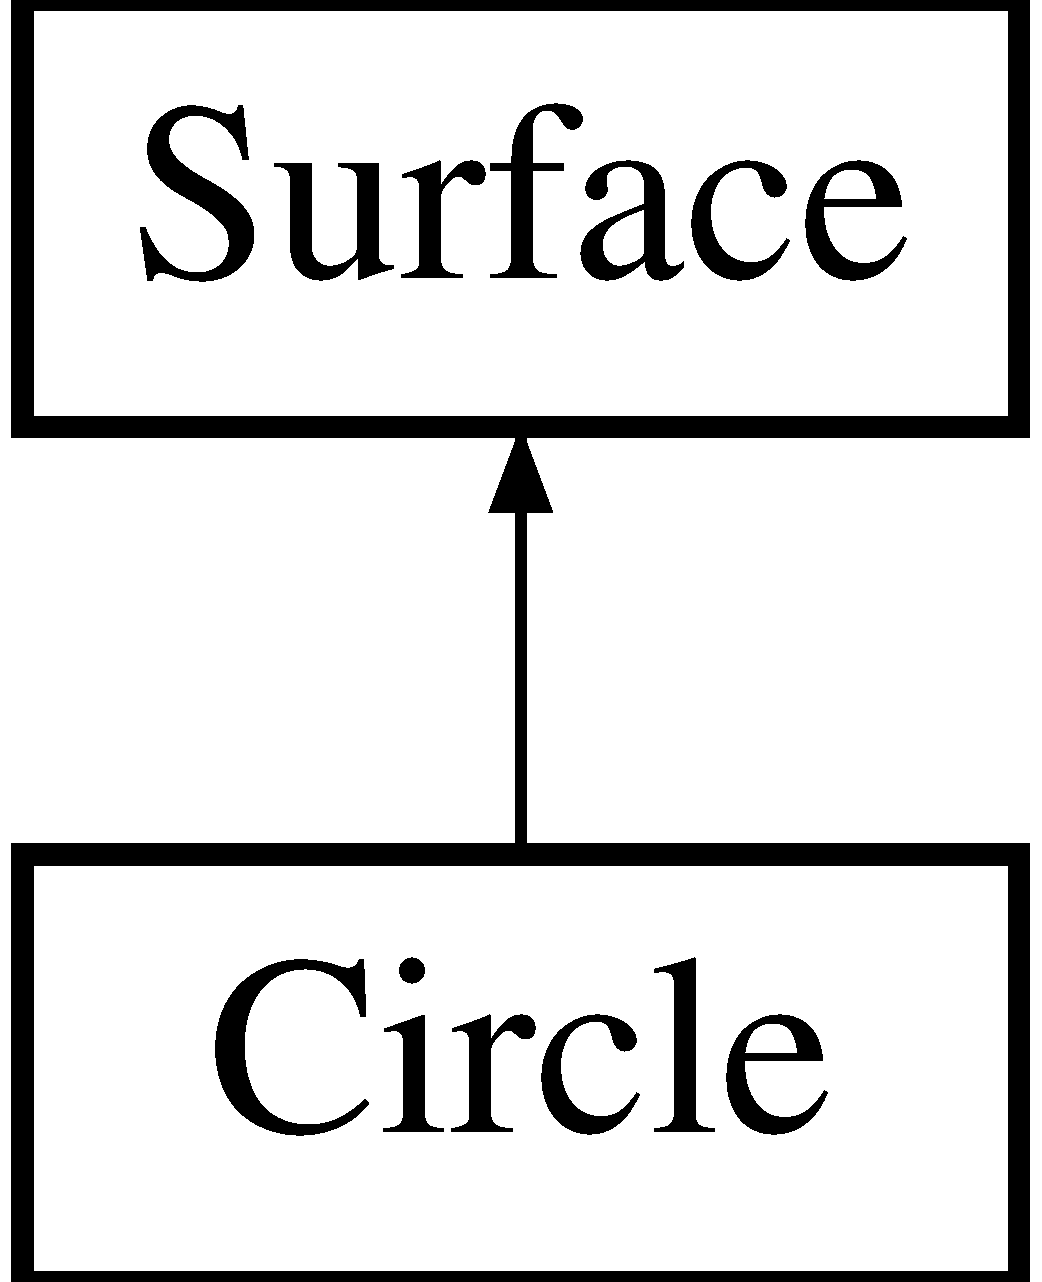
\includegraphics[height=2.000000cm]{classCircle}
\end{center}
\end{figure}
\subsection*{Public Member Functions}
\begin{DoxyCompactItemize}
\item 
\hyperlink{classCircle_ad1ecfcfc7bf34529c6a6d6c448bf70fe}{Circle} ()
\begin{DoxyCompactList}\small\item\em The \hyperlink{classCircle}{Circle} constructor. \end{DoxyCompactList}\item 
\hypertarget{classCircle_ae3f30436e645d73e368e8ee55f8d1650}{virtual \hyperlink{classCircle_ae3f30436e645d73e368e8ee55f8d1650}{$\sim$\-Circle} ()}\label{classCircle_ae3f30436e645d73e368e8ee55f8d1650}

\begin{DoxyCompactList}\small\item\em \hyperlink{classCircle}{Circle} destructor. \end{DoxyCompactList}\item 
float \hyperlink{classCircle_a58d56d258764265600e8c27ecf5c02df}{get\-X0} ()
\begin{DoxyCompactList}\small\item\em Returns the x-\/coordinate of the circle's center. \end{DoxyCompactList}\item 
float \hyperlink{classCircle_ae75c0d7cabbfdd09546ca467ae8a8497}{get\-Y0} ()
\begin{DoxyCompactList}\small\item\em Returns the y-\/coordinate of the circle's center. \end{DoxyCompactList}\item 
float \hyperlink{classCircle_af31f99d2b0d545a0daa936384f5abf6b}{get\-Radius} ()
\begin{DoxyCompactList}\small\item\em Returns the radius of the circle. \end{DoxyCompactList}\item 
void \hyperlink{classCircle_a26f477fd0b422f630d291e7dd1f01d4e}{set\-X0} (float x0)
\begin{DoxyCompactList}\small\item\em Sets the x-\/coordinate of the circle's center. \end{DoxyCompactList}\item 
void \hyperlink{classCircle_aa8a2aabeb95db6b8f7665e2ce21af7ff}{set\-Y0} (float y0)
\begin{DoxyCompactList}\small\item\em Sets the y-\/coordinate of the circle's center. \end{DoxyCompactList}\item 
void \hyperlink{classCircle_af2e568fbc6274720cade0c11521f8fa1}{set\-Radius} (float r)
\begin{DoxyCompactList}\small\item\em Sets the radius of the circle's center. \end{DoxyCompactList}\item 
float \hyperlink{classCircle_a566afb2538f5cae0b863ab3cf6e1f1ab}{compute\-Nearest\-Distance} (\hyperlink{structneutron}{neutron} $\ast$\hyperlink{structneutron}{neutron})
\begin{DoxyCompactList}\small\item\em Computes the nearest distance to the \hyperlink{classCircle}{Circle} along a neutron's trajectory. \end{DoxyCompactList}\item 
bool \hyperlink{classCircle_a129caa61e522c6f0abbbfe5d5d4e7534}{on\-Surface} (\hyperlink{structneutron}{neutron} $\ast$\hyperlink{structneutron}{neutron})
\begin{DoxyCompactList}\small\item\em Checks whether a neutron is on the \hyperlink{classCircle}{Circle}. \end{DoxyCompactList}\end{DoxyCompactItemize}
\subsection*{Protected Attributes}
\begin{DoxyCompactItemize}
\item 
float \hyperlink{classCircle_abe7a680302ea0124535814e97e952fb2}{\-\_\-r}
\item 
float \hyperlink{classCircle_a3ecf4a7fff01cf51ee5416041f0695dc}{\-\_\-r\-\_\-squared}
\item 
float \hyperlink{classCircle_a59739a0da9f81d73cf9b4c380f73320f}{\-\_\-x0}
\item 
float \hyperlink{classCircle_af69cb8c32169429fbe856e701ce14ab5}{\-\_\-y0}
\end{DoxyCompactItemize}


\subsection{Detailed Description}
The \hyperlink{classCircle}{Circle} is the locus of a point equidistant from a fixed point. 

The \hyperlink{classCircle}{Circle} represents a set of points within a given distance from a point in the xy-\/plane called the circle's center. 

\subsection{Constructor \& Destructor Documentation}
\hypertarget{classCircle_ad1ecfcfc7bf34529c6a6d6c448bf70fe}{\index{Circle@{Circle}!Circle@{Circle}}
\index{Circle@{Circle}!Circle@{Circle}}
\subsubsection[{Circle}]{\setlength{\rightskip}{0pt plus 5cm}Circle\-::\-Circle (
\begin{DoxyParamCaption}
{}
\end{DoxyParamCaption}
)}}\label{classCircle_ad1ecfcfc7bf34529c6a6d6c448bf70fe}


The \hyperlink{classCircle}{Circle} constructor. 

Assigns default values for the center of the circle (x=0, y=0) and a radius of 0. 

\subsection{Member Function Documentation}
\hypertarget{classCircle_a566afb2538f5cae0b863ab3cf6e1f1ab}{\index{Circle@{Circle}!compute\-Nearest\-Distance@{compute\-Nearest\-Distance}}
\index{compute\-Nearest\-Distance@{compute\-Nearest\-Distance}!Circle@{Circle}}
\subsubsection[{compute\-Nearest\-Distance}]{\setlength{\rightskip}{0pt plus 5cm}float Circle\-::compute\-Nearest\-Distance (
\begin{DoxyParamCaption}
\item[{{\bf neutron} $\ast$}]{neutron}
\end{DoxyParamCaption}
)\hspace{0.3cm}{\ttfamily [virtual]}}}\label{classCircle_a566afb2538f5cae0b863ab3cf6e1f1ab}


Computes the nearest distance to the \hyperlink{classCircle}{Circle} along a neutron's trajectory. 


\begin{DoxyParams}{Parameters}
{\em neutron} & a pointer to a Neutron struct \\
\hline
\end{DoxyParams}


Implements \hyperlink{classSurface_a3d33dd138200489112a2369eab0b2083}{Surface}.

\hypertarget{classCircle_af31f99d2b0d545a0daa936384f5abf6b}{\index{Circle@{Circle}!get\-Radius@{get\-Radius}}
\index{get\-Radius@{get\-Radius}!Circle@{Circle}}
\subsubsection[{get\-Radius}]{\setlength{\rightskip}{0pt plus 5cm}float Circle\-::get\-Radius (
\begin{DoxyParamCaption}
{}
\end{DoxyParamCaption}
)}}\label{classCircle_af31f99d2b0d545a0daa936384f5abf6b}


Returns the radius of the circle. 

\begin{DoxyReturn}{Returns}
the circle radius 
\end{DoxyReturn}
\hypertarget{classCircle_a58d56d258764265600e8c27ecf5c02df}{\index{Circle@{Circle}!get\-X0@{get\-X0}}
\index{get\-X0@{get\-X0}!Circle@{Circle}}
\subsubsection[{get\-X0}]{\setlength{\rightskip}{0pt plus 5cm}float Circle\-::get\-X0 (
\begin{DoxyParamCaption}
{}
\end{DoxyParamCaption}
)}}\label{classCircle_a58d56d258764265600e8c27ecf5c02df}


Returns the x-\/coordinate of the circle's center. 

\begin{DoxyReturn}{Returns}
the x-\/coordinate of the circle center 
\end{DoxyReturn}
\hypertarget{classCircle_ae75c0d7cabbfdd09546ca467ae8a8497}{\index{Circle@{Circle}!get\-Y0@{get\-Y0}}
\index{get\-Y0@{get\-Y0}!Circle@{Circle}}
\subsubsection[{get\-Y0}]{\setlength{\rightskip}{0pt plus 5cm}float Circle\-::get\-Y0 (
\begin{DoxyParamCaption}
{}
\end{DoxyParamCaption}
)}}\label{classCircle_ae75c0d7cabbfdd09546ca467ae8a8497}


Returns the y-\/coordinate of the circle's center. 

\begin{DoxyReturn}{Returns}
the y-\/coordinate of the circle center 
\end{DoxyReturn}
\hypertarget{classCircle_a129caa61e522c6f0abbbfe5d5d4e7534}{\index{Circle@{Circle}!on\-Surface@{on\-Surface}}
\index{on\-Surface@{on\-Surface}!Circle@{Circle}}
\subsubsection[{on\-Surface}]{\setlength{\rightskip}{0pt plus 5cm}bool Circle\-::on\-Surface (
\begin{DoxyParamCaption}
\item[{{\bf neutron} $\ast$}]{neutron}
\end{DoxyParamCaption}
)\hspace{0.3cm}{\ttfamily [virtual]}}}\label{classCircle_a129caa61e522c6f0abbbfe5d5d4e7534}


Checks whether a neutron is on the \hyperlink{classCircle}{Circle}. 

The threshold used to compute whether or not a neutron is on the on the neutron is 1\-E-\/6 for the difference between the distance between the neutron and the circle center and the radius of the circle. 
\begin{DoxyParams}{Parameters}
{\em neutron} & the neutron of interest \\
\hline
\end{DoxyParams}
\begin{DoxyReturn}{Returns}
true if on the \hyperlink{classXPlane}{X\-Plane}, otherwise false 
\end{DoxyReturn}


Implements \hyperlink{classSurface_acdf69fa01f522393ab504b331d88821a}{Surface}.

\hypertarget{classCircle_af2e568fbc6274720cade0c11521f8fa1}{\index{Circle@{Circle}!set\-Radius@{set\-Radius}}
\index{set\-Radius@{set\-Radius}!Circle@{Circle}}
\subsubsection[{set\-Radius}]{\setlength{\rightskip}{0pt plus 5cm}void Circle\-::set\-Radius (
\begin{DoxyParamCaption}
\item[{float}]{r}
\end{DoxyParamCaption}
)}}\label{classCircle_af2e568fbc6274720cade0c11521f8fa1}


Sets the radius of the circle's center. 


\begin{DoxyParams}{Parameters}
{\em r} & the circle's radius \\
\hline
\end{DoxyParams}
\hypertarget{classCircle_a26f477fd0b422f630d291e7dd1f01d4e}{\index{Circle@{Circle}!set\-X0@{set\-X0}}
\index{set\-X0@{set\-X0}!Circle@{Circle}}
\subsubsection[{set\-X0}]{\setlength{\rightskip}{0pt plus 5cm}void Circle\-::set\-X0 (
\begin{DoxyParamCaption}
\item[{float}]{x0}
\end{DoxyParamCaption}
)}}\label{classCircle_a26f477fd0b422f630d291e7dd1f01d4e}


Sets the x-\/coordinate of the circle's center. 


\begin{DoxyParams}{Parameters}
{\em x0} & the x-\/coordinate of the circle center \\
\hline
\end{DoxyParams}
\hypertarget{classCircle_aa8a2aabeb95db6b8f7665e2ce21af7ff}{\index{Circle@{Circle}!set\-Y0@{set\-Y0}}
\index{set\-Y0@{set\-Y0}!Circle@{Circle}}
\subsubsection[{set\-Y0}]{\setlength{\rightskip}{0pt plus 5cm}void Circle\-::set\-Y0 (
\begin{DoxyParamCaption}
\item[{float}]{y0}
\end{DoxyParamCaption}
)}}\label{classCircle_aa8a2aabeb95db6b8f7665e2ce21af7ff}


Sets the y-\/coordinate of the circle's center. 


\begin{DoxyParams}{Parameters}
{\em y0} & the y-\/coordinate of the circle center \\
\hline
\end{DoxyParams}


\subsection{Member Data Documentation}
\hypertarget{classCircle_abe7a680302ea0124535814e97e952fb2}{\index{Circle@{Circle}!\-\_\-r@{\-\_\-r}}
\index{\-\_\-r@{\-\_\-r}!Circle@{Circle}}
\subsubsection[{\-\_\-r}]{\setlength{\rightskip}{0pt plus 5cm}float Circle\-::\-\_\-r\hspace{0.3cm}{\ttfamily [protected]}}}\label{classCircle_abe7a680302ea0124535814e97e952fb2}
The circle's radius \hypertarget{classCircle_a3ecf4a7fff01cf51ee5416041f0695dc}{\index{Circle@{Circle}!\-\_\-r\-\_\-squared@{\-\_\-r\-\_\-squared}}
\index{\-\_\-r\-\_\-squared@{\-\_\-r\-\_\-squared}!Circle@{Circle}}
\subsubsection[{\-\_\-r\-\_\-squared}]{\setlength{\rightskip}{0pt plus 5cm}float Circle\-::\-\_\-r\-\_\-squared\hspace{0.3cm}{\ttfamily [protected]}}}\label{classCircle_a3ecf4a7fff01cf51ee5416041f0695dc}
The square of the circle's radius \hypertarget{classCircle_a59739a0da9f81d73cf9b4c380f73320f}{\index{Circle@{Circle}!\-\_\-x0@{\-\_\-x0}}
\index{\-\_\-x0@{\-\_\-x0}!Circle@{Circle}}
\subsubsection[{\-\_\-x0}]{\setlength{\rightskip}{0pt plus 5cm}float Circle\-::\-\_\-x0\hspace{0.3cm}{\ttfamily [protected]}}}\label{classCircle_a59739a0da9f81d73cf9b4c380f73320f}
The x-\/coordinate of the circle's center \hypertarget{classCircle_af69cb8c32169429fbe856e701ce14ab5}{\index{Circle@{Circle}!\-\_\-y0@{\-\_\-y0}}
\index{\-\_\-y0@{\-\_\-y0}!Circle@{Circle}}
\subsubsection[{\-\_\-y0}]{\setlength{\rightskip}{0pt plus 5cm}float Circle\-::\-\_\-y0\hspace{0.3cm}{\ttfamily [protected]}}}\label{classCircle_af69cb8c32169429fbe856e701ce14ab5}
The y-\/coordinate of the circle's center 

The documentation for this class was generated from the following files\-:\begin{DoxyCompactItemize}
\item 
\hyperlink{Surface_8h}{Surface.\-h}\item 
Surface.\-cpp\end{DoxyCompactItemize}

\hypertarget{classDerivedTally}{\section{Derived\-Tally Class Reference}
\label{classDerivedTally}\index{Derived\-Tally@{Derived\-Tally}}
}


A class for tallies resulting from tally arithmetic operations.  




{\ttfamily \#include \char`\"{}pinspec/src/\-Tally.\-h\char`\"{}}

Inheritance diagram for Derived\-Tally\-:\begin{figure}[H]
\begin{center}
\leavevmode
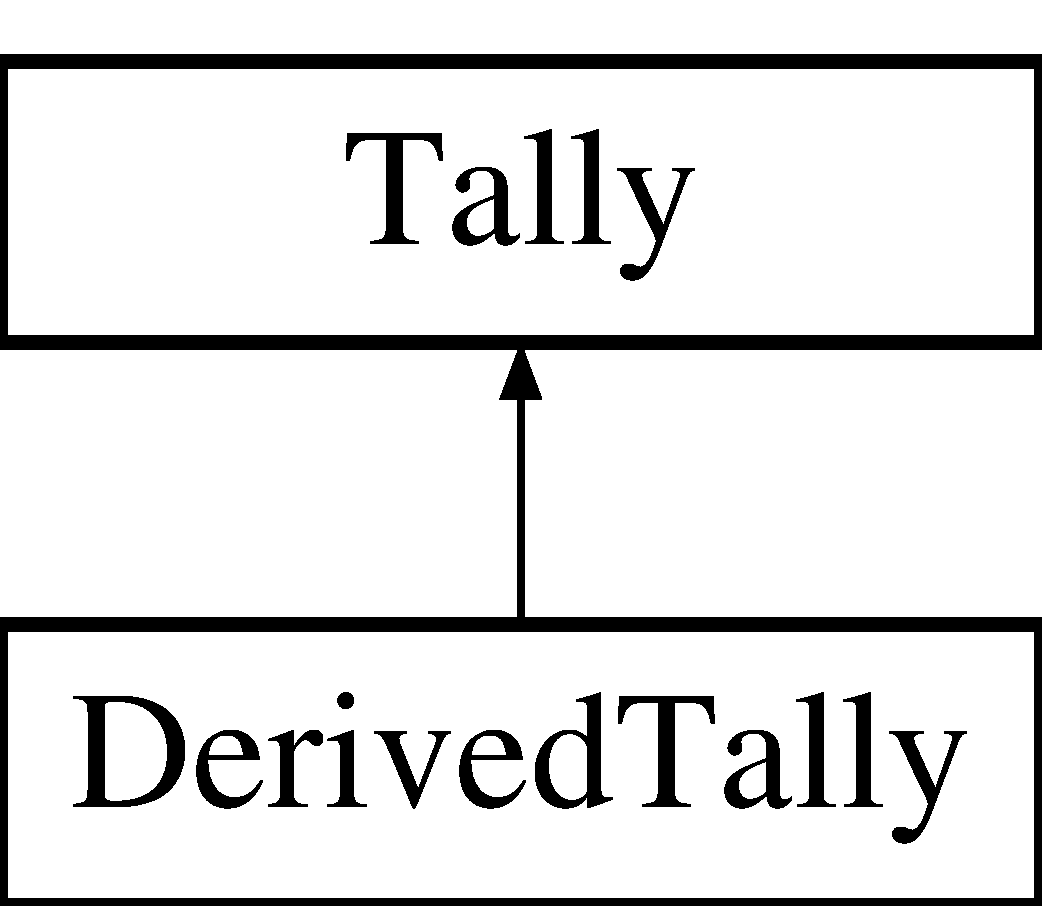
\includegraphics[height=2.000000cm]{classDerivedTally}
\end{center}
\end{figure}
\subsection*{Public Member Functions}
\begin{DoxyCompactItemize}
\item 
\hyperlink{classDerivedTally_a09be94ac5d5d7c0d55cbbbaf48d3585f}{Derived\-Tally} (const char $\ast$tally\-\_\-name=(char $\ast$)\char`\"{}\char`\"{})
\begin{DoxyCompactList}\small\item\em \hyperlink{classDerivedTally}{Derived\-Tally} constructor calls the \hyperlink{classTally}{Tally} constructor and sets the tally domain type to U\-N\-D\-E\-F\-I\-N\-E\-D and the tally type to D\-E\-R\-I\-V\-E\-D. \end{DoxyCompactList}\item 
void \hyperlink{classDerivedTally_a80e9a372015c142cdc74d38b7f281166}{tally} (\hyperlink{structneutron}{neutron} $\ast$\hyperlink{structneutron}{neutron})
\begin{DoxyCompactList}\small\item\em A D\-E\-R\-I\-V\-E\-D tally cannot tally anything, and will throw an exception. \end{DoxyCompactList}\item 
void \hyperlink{classDerivedTally_ab301c71d0c9a36ed455766e5af701398}{set\-Tally\-Name} (char $\ast$tally\-\_\-name)
\begin{DoxyCompactList}\small\item\em Sets the tally name. \end{DoxyCompactList}\item 
void \hyperlink{classDerivedTally_acf9dad27dba5dcbdc598be384c69fa4a}{set\-Tallies} (double $\ast$$\ast$tallies)
\begin{DoxyCompactList}\small\item\em Assigns an array for the tally values. \end{DoxyCompactList}\item 
void \hyperlink{classDerivedTally_a6aabaf89a60ba07a1460518fcbea7990}{set\-Batch\-Mu} (double $\ast$batch\-\_\-mu)
\begin{DoxyCompactList}\small\item\em Assigns an array for the tally batch averages. \end{DoxyCompactList}\item 
void \hyperlink{classDerivedTally_ac70f57c64cea0638308dde7dad25c5d1}{set\-Batch\-Variance} (double $\ast$batch\-\_\-variance)
\begin{DoxyCompactList}\small\item\em Assigns an array for the tally batch variances. \end{DoxyCompactList}\item 
void \hyperlink{classDerivedTally_a43b489858c4b850eff1f7efd75f99d21}{set\-Batch\-Std\-Dev} (double $\ast$batch\-\_\-std\-\_\-dev)
\begin{DoxyCompactList}\small\item\em Assigns an array for the tally batch standard deviations. \end{DoxyCompactList}\item 
void \hyperlink{classDerivedTally_a63b65159121fcb62629a12ce1fb45103}{set\-Batch\-Rel\-Err} (double $\ast$batch\-\_\-rel\-\_\-err)
\begin{DoxyCompactList}\small\item\em Assigns an array for the tally batch relative errors. \end{DoxyCompactList}\item 
void \hyperlink{classDerivedTally_a7ba463b81c010b2dac6495211713dd9d}{set\-Computed\-Batch\-Statistics} (bool computed)
\begin{DoxyCompactList}\small\item\em Assigns whether or not the tally has computed batch statistics. \end{DoxyCompactList}\end{DoxyCompactItemize}
\subsection*{Additional Inherited Members}


\subsection{Detailed Description}
A class for tallies resulting from tally arithmetic operations. 

\subsection{Constructor \& Destructor Documentation}
\hypertarget{classDerivedTally_a09be94ac5d5d7c0d55cbbbaf48d3585f}{\index{Derived\-Tally@{Derived\-Tally}!Derived\-Tally@{Derived\-Tally}}
\index{Derived\-Tally@{Derived\-Tally}!DerivedTally@{Derived\-Tally}}
\subsubsection[{Derived\-Tally}]{\setlength{\rightskip}{0pt plus 5cm}Derived\-Tally\-::\-Derived\-Tally (
\begin{DoxyParamCaption}
\item[{const char $\ast$}]{tally\-\_\-name = {\ttfamily (char$\ast$)\char`\"{}\char`\"{}}}
\end{DoxyParamCaption}
)\hspace{0.3cm}{\ttfamily [inline]}}}\label{classDerivedTally_a09be94ac5d5d7c0d55cbbbaf48d3585f}


\hyperlink{classDerivedTally}{Derived\-Tally} constructor calls the \hyperlink{classTally}{Tally} constructor and sets the tally domain type to U\-N\-D\-E\-F\-I\-N\-E\-D and the tally type to D\-E\-R\-I\-V\-E\-D. 


\begin{DoxyParams}{Parameters}
{\em tally\-\_\-name} & a character array for the tally name (optional) \\
\hline
\end{DoxyParams}


\subsection{Member Function Documentation}
\hypertarget{classDerivedTally_a6aabaf89a60ba07a1460518fcbea7990}{\index{Derived\-Tally@{Derived\-Tally}!set\-Batch\-Mu@{set\-Batch\-Mu}}
\index{set\-Batch\-Mu@{set\-Batch\-Mu}!DerivedTally@{Derived\-Tally}}
\subsubsection[{set\-Batch\-Mu}]{\setlength{\rightskip}{0pt plus 5cm}void Derived\-Tally\-::set\-Batch\-Mu (
\begin{DoxyParamCaption}
\item[{double $\ast$}]{batch\-\_\-mu}
\end{DoxyParamCaption}
)}}\label{classDerivedTally_a6aabaf89a60ba07a1460518fcbea7990}


Assigns an array for the tally batch averages. 


\begin{DoxyParams}{Parameters}
{\em batch\-\_\-mu} & an array of tally averages \\
\hline
\end{DoxyParams}
\hypertarget{classDerivedTally_a63b65159121fcb62629a12ce1fb45103}{\index{Derived\-Tally@{Derived\-Tally}!set\-Batch\-Rel\-Err@{set\-Batch\-Rel\-Err}}
\index{set\-Batch\-Rel\-Err@{set\-Batch\-Rel\-Err}!DerivedTally@{Derived\-Tally}}
\subsubsection[{set\-Batch\-Rel\-Err}]{\setlength{\rightskip}{0pt plus 5cm}void Derived\-Tally\-::set\-Batch\-Rel\-Err (
\begin{DoxyParamCaption}
\item[{double $\ast$}]{batch\-\_\-rel\-\_\-err}
\end{DoxyParamCaption}
)}}\label{classDerivedTally_a63b65159121fcb62629a12ce1fb45103}


Assigns an array for the tally batch relative errors. 


\begin{DoxyParams}{Parameters}
{\em batch\-\_\-rel\-\_\-err} & an array of tally relative errors \\
\hline
\end{DoxyParams}
\hypertarget{classDerivedTally_a43b489858c4b850eff1f7efd75f99d21}{\index{Derived\-Tally@{Derived\-Tally}!set\-Batch\-Std\-Dev@{set\-Batch\-Std\-Dev}}
\index{set\-Batch\-Std\-Dev@{set\-Batch\-Std\-Dev}!DerivedTally@{Derived\-Tally}}
\subsubsection[{set\-Batch\-Std\-Dev}]{\setlength{\rightskip}{0pt plus 5cm}void Derived\-Tally\-::set\-Batch\-Std\-Dev (
\begin{DoxyParamCaption}
\item[{double $\ast$}]{batch\-\_\-std\-\_\-dev}
\end{DoxyParamCaption}
)}}\label{classDerivedTally_a43b489858c4b850eff1f7efd75f99d21}


Assigns an array for the tally batch standard deviations. 


\begin{DoxyParams}{Parameters}
{\em batch\-\_\-std\-\_\-dev} & an array of tally standard deviations \\
\hline
\end{DoxyParams}
\hypertarget{classDerivedTally_ac70f57c64cea0638308dde7dad25c5d1}{\index{Derived\-Tally@{Derived\-Tally}!set\-Batch\-Variance@{set\-Batch\-Variance}}
\index{set\-Batch\-Variance@{set\-Batch\-Variance}!DerivedTally@{Derived\-Tally}}
\subsubsection[{set\-Batch\-Variance}]{\setlength{\rightskip}{0pt plus 5cm}void Derived\-Tally\-::set\-Batch\-Variance (
\begin{DoxyParamCaption}
\item[{double $\ast$}]{batch\-\_\-variance}
\end{DoxyParamCaption}
)}}\label{classDerivedTally_ac70f57c64cea0638308dde7dad25c5d1}


Assigns an array for the tally batch variances. 


\begin{DoxyParams}{Parameters}
{\em batch\-\_\-variance} & an array of tally variances \\
\hline
\end{DoxyParams}
\hypertarget{classDerivedTally_a7ba463b81c010b2dac6495211713dd9d}{\index{Derived\-Tally@{Derived\-Tally}!set\-Computed\-Batch\-Statistics@{set\-Computed\-Batch\-Statistics}}
\index{set\-Computed\-Batch\-Statistics@{set\-Computed\-Batch\-Statistics}!DerivedTally@{Derived\-Tally}}
\subsubsection[{set\-Computed\-Batch\-Statistics}]{\setlength{\rightskip}{0pt plus 5cm}void Derived\-Tally\-::set\-Computed\-Batch\-Statistics (
\begin{DoxyParamCaption}
\item[{bool}]{computed}
\end{DoxyParamCaption}
)}}\label{classDerivedTally_a7ba463b81c010b2dac6495211713dd9d}


Assigns whether or not the tally has computed batch statistics. 


\begin{DoxyParams}{Parameters}
{\em computed} & true if batch statistics are computed; otherwise false \\
\hline
\end{DoxyParams}
\hypertarget{classDerivedTally_acf9dad27dba5dcbdc598be384c69fa4a}{\index{Derived\-Tally@{Derived\-Tally}!set\-Tallies@{set\-Tallies}}
\index{set\-Tallies@{set\-Tallies}!DerivedTally@{Derived\-Tally}}
\subsubsection[{set\-Tallies}]{\setlength{\rightskip}{0pt plus 5cm}void Derived\-Tally\-::set\-Tallies (
\begin{DoxyParamCaption}
\item[{double $\ast$$\ast$}]{tallies}
\end{DoxyParamCaption}
)}}\label{classDerivedTally_acf9dad27dba5dcbdc598be384c69fa4a}


Assigns an array for the tally values. 


\begin{DoxyParams}{Parameters}
{\em tallies} & an array of tally values \\
\hline
\end{DoxyParams}
\hypertarget{classDerivedTally_ab301c71d0c9a36ed455766e5af701398}{\index{Derived\-Tally@{Derived\-Tally}!set\-Tally\-Name@{set\-Tally\-Name}}
\index{set\-Tally\-Name@{set\-Tally\-Name}!DerivedTally@{Derived\-Tally}}
\subsubsection[{set\-Tally\-Name}]{\setlength{\rightskip}{0pt plus 5cm}void Derived\-Tally\-::set\-Tally\-Name (
\begin{DoxyParamCaption}
\item[{char $\ast$}]{tally\-\_\-name}
\end{DoxyParamCaption}
)}}\label{classDerivedTally_ab301c71d0c9a36ed455766e5af701398}


Sets the tally name. 


\begin{DoxyParams}{Parameters}
{\em tally\-\_\-name} & the name of the tally. \\
\hline
\end{DoxyParams}
\hypertarget{classDerivedTally_a80e9a372015c142cdc74d38b7f281166}{\index{Derived\-Tally@{Derived\-Tally}!tally@{tally}}
\index{tally@{tally}!DerivedTally@{Derived\-Tally}}
\subsubsection[{tally}]{\setlength{\rightskip}{0pt plus 5cm}void Derived\-Tally\-::tally (
\begin{DoxyParamCaption}
\item[{{\bf neutron} $\ast$}]{neutron}
\end{DoxyParamCaption}
)\hspace{0.3cm}{\ttfamily [virtual]}}}\label{classDerivedTally_a80e9a372015c142cdc74d38b7f281166}


A D\-E\-R\-I\-V\-E\-D tally cannot tally anything, and will throw an exception. 


\begin{DoxyParams}{Parameters}
{\em neutron} & the neutron of interest \\
\hline
\end{DoxyParams}


Implements \hyperlink{classTally_afb566ef038a61e2449311f2ae95e862e}{Tally}.



The documentation for this class was generated from the following files\-:\begin{DoxyCompactItemize}
\item 
\hyperlink{Tally_8h}{Tally.\-h}\item 
Tally.\-cpp\end{DoxyCompactItemize}

\hypertarget{classFissioner}{\section{Fissioner Class Reference}
\label{classFissioner}\index{Fissioner@{Fissioner}}
}


The \hyperlink{classFissioner}{Fissioner} represents the physics of fission neutron emission.  




{\ttfamily \#include \char`\"{}pinspec/src/\-Fissioner.\-h\char`\"{}}

\subsection*{Public Member Functions}
\begin{DoxyCompactItemize}
\item 
\hyperlink{classFissioner_afcd97a27d994cf3fefb474c9f5887e79}{Fissioner} ()
\begin{DoxyCompactList}\small\item\em Default \hyperlink{classFissioner}{Fissioner} constructor. \end{DoxyCompactList}\item 
\hypertarget{classFissioner_a5b5045b1de9a25a6022aec9124a1b024}{virtual \hyperlink{classFissioner_a5b5045b1de9a25a6022aec9124a1b024}{$\sim$\-Fissioner} ()}\label{classFissioner_a5b5045b1de9a25a6022aec9124a1b024}

\begin{DoxyCompactList}\small\item\em \hyperlink{classFissioner}{Fissioner} destructor deallocates memory for C\-D\-F arrays. \end{DoxyCompactList}\item 
int \hyperlink{classFissioner_a32207d324d2859dcded929d646305425}{get\-Num\-Bins} ()
\begin{DoxyCompactList}\small\item\em Returns the number of bins that the \hyperlink{classFissioner}{Fissioner} uses for the C\-D\-F. \end{DoxyCompactList}\item 
void \hyperlink{classFissioner_a0ccf4ae781088313fd20975aa8d9d789}{set\-Num\-Bins} (int num\-\_\-bins)
\begin{DoxyCompactList}\small\item\em Sets the number of bins that we wish to use for the C\-D\-F. \end{DoxyCompactList}\item 
void \hyperlink{classFissioner_a77c0acd5b3cc8a9b58a7a0fb4182479d}{set\-E\-Max} (float E\-\_\-max)
\begin{DoxyCompactList}\small\item\em Sets the maximum energy value for the C\-D\-F. \end{DoxyCompactList}\item 
\hypertarget{classFissioner_a7e5dd36d86e2b9e026d65bfbc152210b}{void \hyperlink{classFissioner_a7e5dd36d86e2b9e026d65bfbc152210b}{build\-C\-D\-F} ()}\label{classFissioner_a7e5dd36d86e2b9e026d65bfbc152210b}

\begin{DoxyCompactList}\small\item\em Builds the C\-D\-F of the Watt Spectrum. \end{DoxyCompactList}\item 
float \hyperlink{classFissioner_a0d7eec9e2367c433a3dff894b86066af}{watt\-Spectrum} (float energy)
\begin{DoxyCompactList}\small\item\em Returns the chi value for a given energy from the Watt spectrum. \end{DoxyCompactList}\item 
float \hyperlink{classFissioner_a7d4ead1d590eecfc19e7a57361f1c4d7}{emit\-Neutron\-Me\-V} ()
\begin{DoxyCompactList}\small\item\em Sample the \hyperlink{classFissioner}{Fissioner}'s C\-D\-F and return a neutron energy from fission. \end{DoxyCompactList}\item 
float \hyperlink{classFissioner_ab60b9ea50cf7d8b1b1a2b7e5a134ee55}{emit\-Neutrone\-V} ()
\begin{DoxyCompactList}\small\item\em Sample the \hyperlink{classFissioner}{Fissioner}'s C\-D\-F and return a neutron energy from fission. \end{DoxyCompactList}\item 
void \hyperlink{classFissioner_a6df11ab0fc579364199a88e72d60f666}{retrieve\-C\-D\-F} (float $\ast$cdf, int num\-\_\-bins)
\begin{DoxyCompactList}\small\item\em Fills an input array with the \hyperlink{classFissioner}{Fissioner}'s C\-D\-F values. \end{DoxyCompactList}\item 
void \hyperlink{classFissioner_a62bbe8c05eea905ec6aef328bbab8da8}{retrieve\-C\-D\-F\-Energies} (float $\ast$cdf\-\_\-energies, int num\-\_\-bins)
\begin{DoxyCompactList}\small\item\em Fills an input array with the \hyperlink{classFissioner}{Fissioner}'s C\-D\-F energies. \end{DoxyCompactList}\end{DoxyCompactItemize}


\subsection{Detailed Description}
The \hyperlink{classFissioner}{Fissioner} represents the physics of fission neutron emission. 

The \hyperlink{classFissioner}{Fissioner} class contains a cumulative distribution function (C\-D\-F) for the chi spectrum of fission neutron energies. The \hyperlink{classFissioner}{Fissioner} can stochastically sample from the C\-D\-F to generate the neutron fission emisson spectrum. The Watt spectrum given in the \char`\"{}\-Fundamentals of Nuclear Reactor Physics\char`\"{}, E. E. Lewis is used to generate the C\-D\-F\-:

$ \chi = 0.453 * exp(-1.036E) * sinh(sqrt(2.29E)) $ 

\subsection{Constructor \& Destructor Documentation}
\hypertarget{classFissioner_afcd97a27d994cf3fefb474c9f5887e79}{\index{Fissioner@{Fissioner}!Fissioner@{Fissioner}}
\index{Fissioner@{Fissioner}!Fissioner@{Fissioner}}
\subsubsection[{Fissioner}]{\setlength{\rightskip}{0pt plus 5cm}Fissioner\-::\-Fissioner (
\begin{DoxyParamCaption}
{}
\end{DoxyParamCaption}
)}}\label{classFissioner_afcd97a27d994cf3fefb474c9f5887e79}


Default \hyperlink{classFissioner}{Fissioner} constructor. 

Initializes the \hyperlink{classFissioner}{Fissioner} with 1\-E5 bins and a maximum emission energy of 20 Me\-V. 

\subsection{Member Function Documentation}
\hypertarget{classFissioner_ab60b9ea50cf7d8b1b1a2b7e5a134ee55}{\index{Fissioner@{Fissioner}!emit\-Neutrone\-V@{emit\-Neutrone\-V}}
\index{emit\-Neutrone\-V@{emit\-Neutrone\-V}!Fissioner@{Fissioner}}
\subsubsection[{emit\-Neutrone\-V}]{\setlength{\rightskip}{0pt plus 5cm}float Fissioner\-::emit\-Neutrone\-V (
\begin{DoxyParamCaption}
{}
\end{DoxyParamCaption}
)}}\label{classFissioner_ab60b9ea50cf7d8b1b1a2b7e5a134ee55}


Sample the \hyperlink{classFissioner}{Fissioner}'s C\-D\-F and return a neutron energy from fission. 

\begin{DoxyReturn}{Returns}
a neutron energy in e\-V 
\end{DoxyReturn}
\begin{DoxySeeAlso}{See Also}
\hyperlink{classFissioner_a7d4ead1d590eecfc19e7a57361f1c4d7}{Fissioner\-::emit\-Neutron\-Me\-V()} 
\end{DoxySeeAlso}
\hypertarget{classFissioner_a7d4ead1d590eecfc19e7a57361f1c4d7}{\index{Fissioner@{Fissioner}!emit\-Neutron\-Me\-V@{emit\-Neutron\-Me\-V}}
\index{emit\-Neutron\-Me\-V@{emit\-Neutron\-Me\-V}!Fissioner@{Fissioner}}
\subsubsection[{emit\-Neutron\-Me\-V}]{\setlength{\rightskip}{0pt plus 5cm}float Fissioner\-::emit\-Neutron\-Me\-V (
\begin{DoxyParamCaption}
{}
\end{DoxyParamCaption}
)}}\label{classFissioner_a7d4ead1d590eecfc19e7a57361f1c4d7}


Sample the \hyperlink{classFissioner}{Fissioner}'s C\-D\-F and return a neutron energy from fission. 

\begin{DoxyReturn}{Returns}
a neutron energy in Me\-V 
\end{DoxyReturn}
\begin{DoxySeeAlso}{See Also}
\hyperlink{classFissioner_ab60b9ea50cf7d8b1b1a2b7e5a134ee55}{Fissioner\-::emit\-Neutrone\-V()} 
\end{DoxySeeAlso}
\hypertarget{classFissioner_a32207d324d2859dcded929d646305425}{\index{Fissioner@{Fissioner}!get\-Num\-Bins@{get\-Num\-Bins}}
\index{get\-Num\-Bins@{get\-Num\-Bins}!Fissioner@{Fissioner}}
\subsubsection[{get\-Num\-Bins}]{\setlength{\rightskip}{0pt plus 5cm}int Fissioner\-::get\-Num\-Bins (
\begin{DoxyParamCaption}
{}
\end{DoxyParamCaption}
)}}\label{classFissioner_a32207d324d2859dcded929d646305425}


Returns the number of bins that the \hyperlink{classFissioner}{Fissioner} uses for the C\-D\-F. 

\begin{DoxyReturn}{Returns}
the number of C\-D\-F bins 
\end{DoxyReturn}
\hypertarget{classFissioner_a6df11ab0fc579364199a88e72d60f666}{\index{Fissioner@{Fissioner}!retrieve\-C\-D\-F@{retrieve\-C\-D\-F}}
\index{retrieve\-C\-D\-F@{retrieve\-C\-D\-F}!Fissioner@{Fissioner}}
\subsubsection[{retrieve\-C\-D\-F}]{\setlength{\rightskip}{0pt plus 5cm}void Fissioner\-::retrieve\-C\-D\-F (
\begin{DoxyParamCaption}
\item[{float $\ast$}]{cdf, }
\item[{int}]{num\-\_\-bins}
\end{DoxyParamCaption}
)}}\label{classFissioner_a6df11ab0fc579364199a88e72d60f666}


Fills an input array with the \hyperlink{classFissioner}{Fissioner}'s C\-D\-F values. 

This class method is a helper function to allow the user to access the C\-D\-F array through in Python via S\-W\-I\-G by inputting a numpy array to this function. For example, a user may use this function in Python as follows\-:

num\-\_\-cdf\-\_\-bins = fissioner.\-get\-Num\-Bins() numpy\-\_\-cdf = numpy.\-zeros(num\-\_\-cdf\-\_\-bins) fissioner.\-retrieve\-C\-D\-F(numpy\-\_\-cdf)


\begin{DoxyParams}{Parameters}
{\em cdf} & an array of the same length as the \hyperlink{classFissioner}{Fissioner}'s C\-D\-F \\
\hline
{\em num\-\_\-bins} & the length of the input array for the C\-D\-F \\
\hline
\end{DoxyParams}
\hypertarget{classFissioner_a62bbe8c05eea905ec6aef328bbab8da8}{\index{Fissioner@{Fissioner}!retrieve\-C\-D\-F\-Energies@{retrieve\-C\-D\-F\-Energies}}
\index{retrieve\-C\-D\-F\-Energies@{retrieve\-C\-D\-F\-Energies}!Fissioner@{Fissioner}}
\subsubsection[{retrieve\-C\-D\-F\-Energies}]{\setlength{\rightskip}{0pt plus 5cm}void Fissioner\-::retrieve\-C\-D\-F\-Energies (
\begin{DoxyParamCaption}
\item[{float $\ast$}]{cdf\-\_\-energies, }
\item[{int}]{num\-\_\-bins}
\end{DoxyParamCaption}
)}}\label{classFissioner_a62bbe8c05eea905ec6aef328bbab8da8}


Fills an input array with the \hyperlink{classFissioner}{Fissioner}'s C\-D\-F energies. 

This class method is a helper function to allow the user to access the C\-D\-F array through in Python via S\-W\-I\-G by inputting a numpy array to this function. For example, a user may use this function in Python as follows\-:

num\-\_\-cdf\-\_\-energies = fissioner.\-get\-Num\-Bins() numpy\-\_\-cdf\-\_\-energies = numpy.\-zeros(num\-\_\-cdf\-\_\-energies) fissioner.\-retrieve\-C\-D\-F(numpy\-\_\-cdf\-\_\-energies)


\begin{DoxyParams}{Parameters}
{\em cdf\-\_\-energies} & an array of the same length as the \hyperlink{classFissioner}{Fissioner}'s C\-D\-F \\
\hline
{\em num\-\_\-bins} & the length of the input array for the C\-D\-F \\
\hline
\end{DoxyParams}
\hypertarget{classFissioner_a77c0acd5b3cc8a9b58a7a0fb4182479d}{\index{Fissioner@{Fissioner}!set\-E\-Max@{set\-E\-Max}}
\index{set\-E\-Max@{set\-E\-Max}!Fissioner@{Fissioner}}
\subsubsection[{set\-E\-Max}]{\setlength{\rightskip}{0pt plus 5cm}void Fissioner\-::set\-E\-Max (
\begin{DoxyParamCaption}
\item[{float}]{E\-\_\-max}
\end{DoxyParamCaption}
)}}\label{classFissioner_a77c0acd5b3cc8a9b58a7a0fb4182479d}


Sets the maximum energy value for the C\-D\-F. 


\begin{DoxyParams}{Parameters}
{\em E\-\_\-max} & the maximum C\-D\-F energy value in Me\-V \\
\hline
\end{DoxyParams}
\hypertarget{classFissioner_a0ccf4ae781088313fd20975aa8d9d789}{\index{Fissioner@{Fissioner}!set\-Num\-Bins@{set\-Num\-Bins}}
\index{set\-Num\-Bins@{set\-Num\-Bins}!Fissioner@{Fissioner}}
\subsubsection[{set\-Num\-Bins}]{\setlength{\rightskip}{0pt plus 5cm}void Fissioner\-::set\-Num\-Bins (
\begin{DoxyParamCaption}
\item[{int}]{num\-\_\-bins}
\end{DoxyParamCaption}
)}}\label{classFissioner_a0ccf4ae781088313fd20975aa8d9d789}


Sets the number of bins that we wish to use for the C\-D\-F. 


\begin{DoxyParams}{Parameters}
{\em num\-\_\-bins} & the number of C\-D\-F bins \\
\hline
\end{DoxyParams}
\hypertarget{classFissioner_a0d7eec9e2367c433a3dff894b86066af}{\index{Fissioner@{Fissioner}!watt\-Spectrum@{watt\-Spectrum}}
\index{watt\-Spectrum@{watt\-Spectrum}!Fissioner@{Fissioner}}
\subsubsection[{watt\-Spectrum}]{\setlength{\rightskip}{0pt plus 5cm}float Fissioner\-::watt\-Spectrum (
\begin{DoxyParamCaption}
\item[{float}]{energy}
\end{DoxyParamCaption}
)}}\label{classFissioner_a0d7eec9e2367c433a3dff894b86066af}


Returns the chi value for a given energy from the Watt spectrum. 


\begin{DoxyParams}{Parameters}
{\em energy} & a fission energy value in Me\-V \\
\hline
\end{DoxyParams}
\begin{DoxyReturn}{Returns}
the value of chi $\chi$ at that energy 
\end{DoxyReturn}


The documentation for this class was generated from the following files\-:\begin{DoxyCompactItemize}
\item 
\hyperlink{Fissioner_8h}{Fissioner.\-h}\item 
Fissioner.\-cpp\end{DoxyCompactItemize}

\hypertarget{classGeometry}{\section{Geometry Class Reference}
\label{classGeometry}\index{Geometry@{Geometry}}
}


The \hyperlink{classGeometry}{Geometry} represents the highest level entity in which a neutron may reside during a P\-I\-N\-S\-P\-E\-C simulaiton. The geometry consists of one or more regions and controls the highest level Monte Carlo kernel.  




{\ttfamily \#include \char`\"{}pinspec/src/\-Geometry.\-h\char`\"{}}

\subsection*{Public Member Functions}
\begin{DoxyCompactItemize}
\item 
\hyperlink{classGeometry_ad2146d68260c035d7236de7638c036de}{Geometry} (\hyperlink{Geometry_8h_af321382c4a8d9fdb71c83382f82fac00}{spatial\-Type} spatial\-\_\-type)
\begin{DoxyCompactList}\small\item\em Geomtery constructor. \end{DoxyCompactList}\item 
\hypertarget{classGeometry_ad55e832122ab3a2833dcaa6507867678}{virtual \hyperlink{classGeometry_ad55e832122ab3a2833dcaa6507867678}{$\sim$\-Geometry} ()}\label{classGeometry_ad55e832122ab3a2833dcaa6507867678}

\begin{DoxyCompactList}\small\item\em Destructor deletes the \hyperlink{classFissioner}{Fissioner} and lets S\-W\-I\-G delete the regions, materials, isotopes and allies during garbage collection. \end{DoxyCompactList}\item 
int \hyperlink{classGeometry_add8ce27223fdd5f038cbbaa4f552a2c1}{get\-Num\-Neutrons\-Per\-Batch} ()
\begin{DoxyCompactList}\small\item\em Returns the number of neutrons per batch for this simulation. \end{DoxyCompactList}\item 
int \hyperlink{classGeometry_a1110957b5b8e1eafdd6f34ffa233d4d1}{get\-Total\-Num\-Neutrons} ()
\begin{DoxyCompactList}\small\item\em Returns the total number of neutrons for this simulation. \end{DoxyCompactList}\item 
int \hyperlink{classGeometry_af45e47614fc0b25fffd16528d17b296c}{get\-Num\-Batches} ()
\begin{DoxyCompactList}\small\item\em Returns the number of batches of neutrons for this simulation. \end{DoxyCompactList}\item 
int \hyperlink{classGeometry_a254abef4b1f2a48e6b75001856e4c233}{get\-Num\-Threads} ()
\begin{DoxyCompactList}\small\item\em Returns the number of parallel threads for this simulation. \end{DoxyCompactList}\item 
\hyperlink{Geometry_8h_af321382c4a8d9fdb71c83382f82fac00}{spatial\-Type} \hyperlink{classGeometry_ac64b1e5ebf43a9538952b20eaf07ef3b}{get\-Spatial\-Type} ()
\begin{DoxyCompactList}\small\item\em Return the spatial type of \hyperlink{classGeometry}{Geometry} (I\-N\-F\-I\-N\-I\-T\-E\-\_\-\-H\-O\-M\-O\-G\-E\-N\-E\-O\-U\-S, H\-O\-M\-O\-G\-E\-N\-E\-O\-U\-S\-\_\-\-E\-Q\-U\-I\-V\-A\-L\-E\-N\-C\-E or H\-E\-T\-E\-R\-O\-G\-E\-N\-E\-O\-U\-S). \end{DoxyCompactList}\item 
float \hyperlink{classGeometry_a662e458bc59ac8390e0c07cea3ab0be8}{get\-Buckling\-Squared} ()
\begin{DoxyCompactList}\small\item\em Returns the square of the geometric buckling for this geometry. \end{DoxyCompactList}\item 
float \hyperlink{classGeometry_a982427d7ad500c703b5348f455b7dced}{get\-Volume} ()
\begin{DoxyCompactList}\small\item\em Returns the total volume occuppied by the geometry. \end{DoxyCompactList}\item 
void \hyperlink{classGeometry_a0160e8eef8ecd7655dc2ddc8f7a46391}{set\-Neutrons\-Per\-Batch} (int num\-\_\-neutrons\-\_\-per\-\_\-batch)
\begin{DoxyCompactList}\small\item\em Sets the number of neutrons per batch for this simulation. \end{DoxyCompactList}\item 
void \hyperlink{classGeometry_ab78e778d1362e38dd9e02514e7ee7019}{set\-Num\-Batches} (int num\-\_\-batches)
\begin{DoxyCompactList}\small\item\em Sets the number of batches for this simulation. \end{DoxyCompactList}\item 
void \hyperlink{classGeometry_a657cb04b0e42bc9a1574a9120c5a6e67}{set\-Num\-Threads} (int num\-\_\-threads)
\begin{DoxyCompactList}\small\item\em Sets the number of batches for this simulation. \end{DoxyCompactList}\item 
void \hyperlink{classGeometry_a52ab88674bf4f90db4fab0899f326a58}{set\-Spatial\-Type} (\hyperlink{Geometry_8h_af321382c4a8d9fdb71c83382f82fac00}{spatial\-Type} spatial\-\_\-type)
\begin{DoxyCompactList}\small\item\em Set the geometry's spatial type (I\-N\-F\-I\-N\-I\-T\-E\-\_\-\-H\-O\-M\-O\-G\-E\-N\-E\-O\-U\-S, H\-O\-M\-O\-G\-E\-N\-E\-O\-U\-S\-\_\-\-E\-Q\-U\-I\-V\-A\-L\-E\-N\-C\-E or H\-E\-T\-E\-R\-O\-G\-E\-N\-E\-O\-U\-S). \end{DoxyCompactList}\item 
void \hyperlink{classGeometry_a0ef3fcbefaf7079ee1667adc3d0dbe54}{set\-Dancoff\-Factor} (float dancoff)
\begin{DoxyCompactList}\small\item\em Sets the dancoff factor and computes the escape cross-\/section, beta, alpha1 and alpha2 parameters used for a two region heterogeneous-\/homogeneous pin cell simulation. \end{DoxyCompactList}\item 
void \hyperlink{classGeometry_a68b1626c22c75914eafdcee252406b62}{add\-Region} (\hyperlink{classRegion}{Region} $\ast$region)
\begin{DoxyCompactList}\small\item\em Adds a new region to the geometry. \end{DoxyCompactList}\item 
void \hyperlink{classGeometry_a81f067e09349731a0b90bdda98b83594}{set\-Buckling\-Squared} (float buckling\-\_\-squared)
\begin{DoxyCompactList}\small\item\em Sets the square of the geometric buckling for the geometry. \end{DoxyCompactList}\item 
void \hyperlink{classGeometry_a32ac1087eeb0f71d4f36b751e65cfe9d}{run\-Monte\-Carlo\-Simulation} ()
\begin{DoxyCompactList}\small\item\em The primary Monte Carlo kernel for a P\-I\-N\-S\-P\-E\-C simulation. \end{DoxyCompactList}\end{DoxyCompactItemize}
\subsection*{Private Member Functions}
\begin{DoxyCompactItemize}
\item 
void \hyperlink{classGeometry_a8cff9ffc1cdeff81b79b1be44bc07727}{initialize\-Prob\-Mod\-Fuel\-Ratios} ()
\begin{DoxyCompactList}\small\item\em Initializes a pre-\/computed array of moderator to fuel first flight probability ratios. \end{DoxyCompactList}\item 
int \hyperlink{classGeometry_a83068853767cd0ac581250f7e2e38981}{get\-Energy\-Grid\-Index} (float energy) const 
\begin{DoxyCompactList}\small\item\em This method returns the index for a certain energy (e\-V) into the uniform lethargy grid of the geometry's first flight probability of travel from moderator to fuel $ p_{mf} $ ratios. \end{DoxyCompactList}\item 
float \hyperlink{classGeometry_aee0db385712e2bc3800028159d61d1ab}{compute\-Fuel\-Fuel\-Collision\-Prob} (\hyperlink{structneutron}{neutron} $\ast$\hyperlink{structneutron}{neutron})
\begin{DoxyCompactList}\small\item\em This function computes the two-\/region fuel-\/to-\/fuel collision probability for a two-\/region pin cell simulation. It uses Carlvik's two-\/term rational model. \end{DoxyCompactList}\item 
float \hyperlink{classGeometry_a1d6e3070b59ce33b1c25d04635889dfb}{compute\-Moderator\-Fuel\-Collision\-Prob} (\hyperlink{structneutron}{neutron} $\ast$\hyperlink{structneutron}{neutron})
\begin{DoxyCompactList}\small\item\em This function computes the two-\/region moderator-\/to-\/fuel collision probability for a two-\/region pin cell simulation. It uses Carlvik's two-\/term rational model. \end{DoxyCompactList}\end{DoxyCompactItemize}
\subsection*{Private Attributes}
\begin{DoxyCompactItemize}
\item 
int \hyperlink{classGeometry_ab2f62b285fd3ebc06114db10a3f50167}{\-\_\-num\-\_\-neutrons\-\_\-per\-\_\-batch}
\item 
int \hyperlink{classGeometry_a600fda86b7f3951331ae486548306407}{\-\_\-num\-\_\-batches}
\item 
int \hyperlink{classGeometry_af78593ff6416ad7fc318e4b8692ed77e}{\-\_\-num\-\_\-threads}
\item 
\hyperlink{Geometry_8h_af321382c4a8d9fdb71c83382f82fac00}{spatial\-Type} \hyperlink{classGeometry_a2e9b473e54caa2c7742b4f676bedf91e}{\-\_\-spatial\-\_\-type}
\item 
\hyperlink{classRegion}{Region} $\ast$ \hyperlink{classGeometry_aad96c277327aa2fb1f512f4678af94f0}{\-\_\-infinite\-\_\-medium}
\item 
\hyperlink{classRegion}{Region} $\ast$ \hyperlink{classGeometry_afca54e88b6d937055fc9ca124db1e17e}{\-\_\-fuel}
\item 
\hyperlink{classRegion}{Region} $\ast$ \hyperlink{classGeometry_a023855a68edb163698d88da928935c4b}{\-\_\-moderator}
\item 
\hyperlink{structneutron}{neutron} $\ast$ \hyperlink{classGeometry_aae2651151b89d9b82c434eaa83edc477}{\-\_\-neutrons}
\item 
\hyperlink{classFissioner}{Fissioner} $\ast$ \hyperlink{classGeometry_a5947cd1c6029329ed188ce4b8a8d4e28}{\-\_\-fissioner}
\item 
float \hyperlink{classGeometry_aedfa5e190e5e87f0a0d84ca48278e019}{\-\_\-dancoff}
\item 
float \hyperlink{classGeometry_a161dd81342c2018dc6af5db732385b67}{\-\_\-sigma\-\_\-e}
\item 
float \hyperlink{classGeometry_a20733d493193d7c75ad9afb454046324}{\-\_\-beta}
\item 
float \hyperlink{classGeometry_a29007358759f00d89a8544539bfb7b75}{\-\_\-alpha1}
\item 
float \hyperlink{classGeometry_a36642c1914426a3bdbcb291497e2c7f8}{\-\_\-alpha2}
\item 
float \hyperlink{classGeometry_aa4c62b0931b1a51effdec42a28e9088f}{\-\_\-buckling\-\_\-squared}
\item 
int \hyperlink{classGeometry_a67baa59c9ac0e8819e5844bcef85442d}{\-\_\-num\-\_\-ratios}
\item 
float $\ast$ \hyperlink{classGeometry_a4bb0c2db80028191a363a79669e2508b}{\-\_\-pmf\-\_\-ratios}
\item 
\hyperlink{Tally_8h_ab7d4ad30f44e9abe7178a76b03887909}{bin\-Spacing\-Types} \hyperlink{classGeometry_a603f3cc50a03607fb94f4ce019235b5a}{\-\_\-scale\-\_\-type}
\item 
float \hyperlink{classGeometry_a274a1e1973986b23507d7c11fb30ea76}{\-\_\-start\-\_\-energy}
\item 
float \hyperlink{classGeometry_a00b1350cc678173b76e8ad06b4916288}{\-\_\-end\-\_\-energy}
\item 
float \hyperlink{classGeometry_a19f967291b5e54888033a1a52a8fc6a5}{\-\_\-delta\-\_\-energy}
\end{DoxyCompactItemize}


\subsection{Detailed Description}
The \hyperlink{classGeometry}{Geometry} represents the highest level entity in which a neutron may reside during a P\-I\-N\-S\-P\-E\-C simulaiton. The geometry consists of one or more regions and controls the highest level Monte Carlo kernel. 

\subsection{Constructor \& Destructor Documentation}
\hypertarget{classGeometry_ad2146d68260c035d7236de7638c036de}{\index{Geometry@{Geometry}!Geometry@{Geometry}}
\index{Geometry@{Geometry}!Geometry@{Geometry}}
\subsubsection[{Geometry}]{\setlength{\rightskip}{0pt plus 5cm}Geometry\-::\-Geometry (
\begin{DoxyParamCaption}
\item[{{\bf spatial\-Type}}]{spatial\-\_\-type}
\end{DoxyParamCaption}
)}}\label{classGeometry_ad2146d68260c035d7236de7638c036de}


Geomtery constructor. 

Sets a default number of neutrons per batch (10,000), number of batches (10) and number of threads (1). 

\subsection{Member Function Documentation}
\hypertarget{classGeometry_a68b1626c22c75914eafdcee252406b62}{\index{Geometry@{Geometry}!add\-Region@{add\-Region}}
\index{add\-Region@{add\-Region}!Geometry@{Geometry}}
\subsubsection[{add\-Region}]{\setlength{\rightskip}{0pt plus 5cm}void Geometry\-::add\-Region (
\begin{DoxyParamCaption}
\item[{{\bf Region} $\ast$}]{region}
\end{DoxyParamCaption}
)}}\label{classGeometry_a68b1626c22c75914eafdcee252406b62}


Adds a new region to the geometry. 

Checks to make sure that the region type (I\-N\-F\-I\-N\-I\-T\-E, F\-U\-E\-L, M\-O\-D\-E\-R\-A\-T\-O\-R) does not conflict with other regions that have already been added to the geometry 
\begin{DoxyParams}{Parameters}
{\em region} & the region to add to the geometry \\
\hline
\end{DoxyParams}
\hypertarget{classGeometry_aee0db385712e2bc3800028159d61d1ab}{\index{Geometry@{Geometry}!compute\-Fuel\-Fuel\-Collision\-Prob@{compute\-Fuel\-Fuel\-Collision\-Prob}}
\index{compute\-Fuel\-Fuel\-Collision\-Prob@{compute\-Fuel\-Fuel\-Collision\-Prob}!Geometry@{Geometry}}
\subsubsection[{compute\-Fuel\-Fuel\-Collision\-Prob}]{\setlength{\rightskip}{0pt plus 5cm}float Geometry\-::compute\-Fuel\-Fuel\-Collision\-Prob (
\begin{DoxyParamCaption}
\item[{{\bf neutron} $\ast$}]{neutron}
\end{DoxyParamCaption}
)\hspace{0.3cm}{\ttfamily [private]}}}\label{classGeometry_aee0db385712e2bc3800028159d61d1ab}


This function computes the two-\/region fuel-\/to-\/fuel collision probability for a two-\/region pin cell simulation. It uses Carlvik's two-\/term rational model. 


\begin{DoxyParams}{Parameters}
{\em neutron} & the neutron of interest \\
\hline
\end{DoxyParams}
\begin{DoxyReturn}{Returns}
the fuel-\/to-\/fuel collision probability at the neutron's energy 
\end{DoxyReturn}
\hypertarget{classGeometry_a1d6e3070b59ce33b1c25d04635889dfb}{\index{Geometry@{Geometry}!compute\-Moderator\-Fuel\-Collision\-Prob@{compute\-Moderator\-Fuel\-Collision\-Prob}}
\index{compute\-Moderator\-Fuel\-Collision\-Prob@{compute\-Moderator\-Fuel\-Collision\-Prob}!Geometry@{Geometry}}
\subsubsection[{compute\-Moderator\-Fuel\-Collision\-Prob}]{\setlength{\rightskip}{0pt plus 5cm}float Geometry\-::compute\-Moderator\-Fuel\-Collision\-Prob (
\begin{DoxyParamCaption}
\item[{{\bf neutron} $\ast$}]{neutron}
\end{DoxyParamCaption}
)\hspace{0.3cm}{\ttfamily [private]}}}\label{classGeometry_a1d6e3070b59ce33b1c25d04635889dfb}


This function computes the two-\/region moderator-\/to-\/fuel collision probability for a two-\/region pin cell simulation. It uses Carlvik's two-\/term rational model. 


\begin{DoxyParams}{Parameters}
{\em neutron} & the neutron of interest \\
\hline
\end{DoxyParams}
\begin{DoxyReturn}{Returns}
the moderator-\/to-\/fuel collision probability at the neutron's energy 
\end{DoxyReturn}
\hypertarget{classGeometry_a662e458bc59ac8390e0c07cea3ab0be8}{\index{Geometry@{Geometry}!get\-Buckling\-Squared@{get\-Buckling\-Squared}}
\index{get\-Buckling\-Squared@{get\-Buckling\-Squared}!Geometry@{Geometry}}
\subsubsection[{get\-Buckling\-Squared}]{\setlength{\rightskip}{0pt plus 5cm}float Geometry\-::get\-Buckling\-Squared (
\begin{DoxyParamCaption}
{}
\end{DoxyParamCaption}
)}}\label{classGeometry_a662e458bc59ac8390e0c07cea3ab0be8}


Returns the square of the geometric buckling for this geometry. 

\begin{DoxyReturn}{Returns}
the square of the geometric buckling 
\end{DoxyReturn}
\hypertarget{classGeometry_a83068853767cd0ac581250f7e2e38981}{\index{Geometry@{Geometry}!get\-Energy\-Grid\-Index@{get\-Energy\-Grid\-Index}}
\index{get\-Energy\-Grid\-Index@{get\-Energy\-Grid\-Index}!Geometry@{Geometry}}
\subsubsection[{get\-Energy\-Grid\-Index}]{\setlength{\rightskip}{0pt plus 5cm}int Geometry\-::get\-Energy\-Grid\-Index (
\begin{DoxyParamCaption}
\item[{float}]{energy}
\end{DoxyParamCaption}
) const\hspace{0.3cm}{\ttfamily [inline]}, {\ttfamily [private]}}}\label{classGeometry_a83068853767cd0ac581250f7e2e38981}


This method returns the index for a certain energy (e\-V) into the uniform lethargy grid of the geometry's first flight probability of travel from moderator to fuel $ p_{mf} $ ratios. 


\begin{DoxyParams}{Parameters}
{\em energy} & the energy (e\-V) of interest \\
\hline
\end{DoxyParams}
\begin{DoxyReturn}{Returns}
the index into the uniform lethargy grid 
\end{DoxyReturn}
\hypertarget{classGeometry_af45e47614fc0b25fffd16528d17b296c}{\index{Geometry@{Geometry}!get\-Num\-Batches@{get\-Num\-Batches}}
\index{get\-Num\-Batches@{get\-Num\-Batches}!Geometry@{Geometry}}
\subsubsection[{get\-Num\-Batches}]{\setlength{\rightskip}{0pt plus 5cm}int Geometry\-::get\-Num\-Batches (
\begin{DoxyParamCaption}
{}
\end{DoxyParamCaption}
)}}\label{classGeometry_af45e47614fc0b25fffd16528d17b296c}


Returns the number of batches of neutrons for this simulation. 

\begin{DoxyReturn}{Returns}
the number of batches 
\end{DoxyReturn}
\hypertarget{classGeometry_add8ce27223fdd5f038cbbaa4f552a2c1}{\index{Geometry@{Geometry}!get\-Num\-Neutrons\-Per\-Batch@{get\-Num\-Neutrons\-Per\-Batch}}
\index{get\-Num\-Neutrons\-Per\-Batch@{get\-Num\-Neutrons\-Per\-Batch}!Geometry@{Geometry}}
\subsubsection[{get\-Num\-Neutrons\-Per\-Batch}]{\setlength{\rightskip}{0pt plus 5cm}int Geometry\-::get\-Num\-Neutrons\-Per\-Batch (
\begin{DoxyParamCaption}
{}
\end{DoxyParamCaption}
)}}\label{classGeometry_add8ce27223fdd5f038cbbaa4f552a2c1}


Returns the number of neutrons per batch for this simulation. 

\begin{DoxyReturn}{Returns}
the number of neutrons per batch 
\end{DoxyReturn}
\hypertarget{classGeometry_a254abef4b1f2a48e6b75001856e4c233}{\index{Geometry@{Geometry}!get\-Num\-Threads@{get\-Num\-Threads}}
\index{get\-Num\-Threads@{get\-Num\-Threads}!Geometry@{Geometry}}
\subsubsection[{get\-Num\-Threads}]{\setlength{\rightskip}{0pt plus 5cm}int Geometry\-::get\-Num\-Threads (
\begin{DoxyParamCaption}
{}
\end{DoxyParamCaption}
)}}\label{classGeometry_a254abef4b1f2a48e6b75001856e4c233}


Returns the number of parallel threads for this simulation. 

\begin{DoxyReturn}{Returns}
the number of threads 
\end{DoxyReturn}
\hypertarget{classGeometry_ac64b1e5ebf43a9538952b20eaf07ef3b}{\index{Geometry@{Geometry}!get\-Spatial\-Type@{get\-Spatial\-Type}}
\index{get\-Spatial\-Type@{get\-Spatial\-Type}!Geometry@{Geometry}}
\subsubsection[{get\-Spatial\-Type}]{\setlength{\rightskip}{0pt plus 5cm}{\bf spatial\-Type} Geometry\-::get\-Spatial\-Type (
\begin{DoxyParamCaption}
{}
\end{DoxyParamCaption}
)}}\label{classGeometry_ac64b1e5ebf43a9538952b20eaf07ef3b}


Return the spatial type of \hyperlink{classGeometry}{Geometry} (I\-N\-F\-I\-N\-I\-T\-E\-\_\-\-H\-O\-M\-O\-G\-E\-N\-E\-O\-U\-S, H\-O\-M\-O\-G\-E\-N\-E\-O\-U\-S\-\_\-\-E\-Q\-U\-I\-V\-A\-L\-E\-N\-C\-E or H\-E\-T\-E\-R\-O\-G\-E\-N\-E\-O\-U\-S). 

\begin{DoxyReturn}{Returns}
the spatial type 
\end{DoxyReturn}
\hypertarget{classGeometry_a1110957b5b8e1eafdd6f34ffa233d4d1}{\index{Geometry@{Geometry}!get\-Total\-Num\-Neutrons@{get\-Total\-Num\-Neutrons}}
\index{get\-Total\-Num\-Neutrons@{get\-Total\-Num\-Neutrons}!Geometry@{Geometry}}
\subsubsection[{get\-Total\-Num\-Neutrons}]{\setlength{\rightskip}{0pt plus 5cm}int Geometry\-::get\-Total\-Num\-Neutrons (
\begin{DoxyParamCaption}
{}
\end{DoxyParamCaption}
)}}\label{classGeometry_a1110957b5b8e1eafdd6f34ffa233d4d1}


Returns the total number of neutrons for this simulation. 

\begin{DoxyReturn}{Returns}
the total number of neutrons for this simulation 
\end{DoxyReturn}
\hypertarget{classGeometry_a982427d7ad500c703b5348f455b7dced}{\index{Geometry@{Geometry}!get\-Volume@{get\-Volume}}
\index{get\-Volume@{get\-Volume}!Geometry@{Geometry}}
\subsubsection[{get\-Volume}]{\setlength{\rightskip}{0pt plus 5cm}float Geometry\-::get\-Volume (
\begin{DoxyParamCaption}
{}
\end{DoxyParamCaption}
)}}\label{classGeometry_a982427d7ad500c703b5348f455b7dced}


Returns the total volume occuppied by the geometry. 

\begin{DoxyReturn}{Returns}
The total volume for the geometry 
\end{DoxyReturn}
\hypertarget{classGeometry_a8cff9ffc1cdeff81b79b1be44bc07727}{\index{Geometry@{Geometry}!initialize\-Prob\-Mod\-Fuel\-Ratios@{initialize\-Prob\-Mod\-Fuel\-Ratios}}
\index{initialize\-Prob\-Mod\-Fuel\-Ratios@{initialize\-Prob\-Mod\-Fuel\-Ratios}!Geometry@{Geometry}}
\subsubsection[{initialize\-Prob\-Mod\-Fuel\-Ratios}]{\setlength{\rightskip}{0pt plus 5cm}void Geometry\-::initialize\-Prob\-Mod\-Fuel\-Ratios (
\begin{DoxyParamCaption}
{}
\end{DoxyParamCaption}
)\hspace{0.3cm}{\ttfamily [private]}}}\label{classGeometry_a8cff9ffc1cdeff81b79b1be44bc07727}


Initializes a pre-\/computed array of moderator to fuel first flight probability ratios. 

The pre-\/computaiton of the ratios is an optimization to save time for the homogeneous-\/heterogeneous equivalence geometry type. \hypertarget{classGeometry_a32ac1087eeb0f71d4f36b751e65cfe9d}{\index{Geometry@{Geometry}!run\-Monte\-Carlo\-Simulation@{run\-Monte\-Carlo\-Simulation}}
\index{run\-Monte\-Carlo\-Simulation@{run\-Monte\-Carlo\-Simulation}!Geometry@{Geometry}}
\subsubsection[{run\-Monte\-Carlo\-Simulation}]{\setlength{\rightskip}{0pt plus 5cm}void Geometry\-::run\-Monte\-Carlo\-Simulation (
\begin{DoxyParamCaption}
{}
\end{DoxyParamCaption}
)}}\label{classGeometry_a32ac1087eeb0f71d4f36b751e65cfe9d}


The primary Monte Carlo kernel for a P\-I\-N\-S\-P\-E\-C simulation. 

This method executes an appropriate Monte Carlo kernel depending on the geometry's spatial type. This method loops over batches and neutrons and collides each neutron in the appropriate region until it is absorbed, while tallying all user-\/specific quanties throughout. \hypertarget{classGeometry_a81f067e09349731a0b90bdda98b83594}{\index{Geometry@{Geometry}!set\-Buckling\-Squared@{set\-Buckling\-Squared}}
\index{set\-Buckling\-Squared@{set\-Buckling\-Squared}!Geometry@{Geometry}}
\subsubsection[{set\-Buckling\-Squared}]{\setlength{\rightskip}{0pt plus 5cm}void Geometry\-::set\-Buckling\-Squared (
\begin{DoxyParamCaption}
\item[{float}]{buckling\-\_\-squared}
\end{DoxyParamCaption}
)}}\label{classGeometry_a81f067e09349731a0b90bdda98b83594}


Sets the square of the geometric buckling for the geometry. 


\begin{DoxyParams}{Parameters}
{\em buckling\-\_\-squared} & the square of the geometric buckling \\
\hline
\end{DoxyParams}
\hypertarget{classGeometry_a0ef3fcbefaf7079ee1667adc3d0dbe54}{\index{Geometry@{Geometry}!set\-Dancoff\-Factor@{set\-Dancoff\-Factor}}
\index{set\-Dancoff\-Factor@{set\-Dancoff\-Factor}!Geometry@{Geometry}}
\subsubsection[{set\-Dancoff\-Factor}]{\setlength{\rightskip}{0pt plus 5cm}void Geometry\-::set\-Dancoff\-Factor (
\begin{DoxyParamCaption}
\item[{float}]{dancoff}
\end{DoxyParamCaption}
)}}\label{classGeometry_a0ef3fcbefaf7079ee1667adc3d0dbe54}


Sets the dancoff factor and computes the escape cross-\/section, beta, alpha1 and alpha2 parameters used for a two region heterogeneous-\/homogeneous pin cell simulation. 


\begin{DoxyParams}{Parameters}
{\em dancoff} & the dancoff factor \\
\hline
\end{DoxyParams}
\hypertarget{classGeometry_a0160e8eef8ecd7655dc2ddc8f7a46391}{\index{Geometry@{Geometry}!set\-Neutrons\-Per\-Batch@{set\-Neutrons\-Per\-Batch}}
\index{set\-Neutrons\-Per\-Batch@{set\-Neutrons\-Per\-Batch}!Geometry@{Geometry}}
\subsubsection[{set\-Neutrons\-Per\-Batch}]{\setlength{\rightskip}{0pt plus 5cm}void Geometry\-::set\-Neutrons\-Per\-Batch (
\begin{DoxyParamCaption}
\item[{int}]{num\-\_\-neutrons\-\_\-per\-\_\-batch}
\end{DoxyParamCaption}
)}}\label{classGeometry_a0160e8eef8ecd7655dc2ddc8f7a46391}


Sets the number of neutrons per batch for this simulation. 


\begin{DoxyParams}{Parameters}
{\em num\-\_\-neutrons\-\_\-per\-\_\-batch} & the number of neutrons per batch \\
\hline
\end{DoxyParams}
\hypertarget{classGeometry_ab78e778d1362e38dd9e02514e7ee7019}{\index{Geometry@{Geometry}!set\-Num\-Batches@{set\-Num\-Batches}}
\index{set\-Num\-Batches@{set\-Num\-Batches}!Geometry@{Geometry}}
\subsubsection[{set\-Num\-Batches}]{\setlength{\rightskip}{0pt plus 5cm}void Geometry\-::set\-Num\-Batches (
\begin{DoxyParamCaption}
\item[{int}]{num\-\_\-batches}
\end{DoxyParamCaption}
)}}\label{classGeometry_ab78e778d1362e38dd9e02514e7ee7019}


Sets the number of batches for this simulation. 


\begin{DoxyParams}{Parameters}
{\em num\-\_\-batches} & the number of batches \\
\hline
\end{DoxyParams}
\hypertarget{classGeometry_a657cb04b0e42bc9a1574a9120c5a6e67}{\index{Geometry@{Geometry}!set\-Num\-Threads@{set\-Num\-Threads}}
\index{set\-Num\-Threads@{set\-Num\-Threads}!Geometry@{Geometry}}
\subsubsection[{set\-Num\-Threads}]{\setlength{\rightskip}{0pt plus 5cm}void Geometry\-::set\-Num\-Threads (
\begin{DoxyParamCaption}
\item[{int}]{num\-\_\-threads}
\end{DoxyParamCaption}
)}}\label{classGeometry_a657cb04b0e42bc9a1574a9120c5a6e67}


Sets the number of batches for this simulation. 


\begin{DoxyParams}{Parameters}
{\em num\-\_\-threads} & the number of batches \\
\hline
\end{DoxyParams}
\hypertarget{classGeometry_a52ab88674bf4f90db4fab0899f326a58}{\index{Geometry@{Geometry}!set\-Spatial\-Type@{set\-Spatial\-Type}}
\index{set\-Spatial\-Type@{set\-Spatial\-Type}!Geometry@{Geometry}}
\subsubsection[{set\-Spatial\-Type}]{\setlength{\rightskip}{0pt plus 5cm}void Geometry\-::set\-Spatial\-Type (
\begin{DoxyParamCaption}
\item[{{\bf spatial\-Type}}]{spatial\-\_\-type}
\end{DoxyParamCaption}
)}}\label{classGeometry_a52ab88674bf4f90db4fab0899f326a58}


Set the geometry's spatial type (I\-N\-F\-I\-N\-I\-T\-E\-\_\-\-H\-O\-M\-O\-G\-E\-N\-E\-O\-U\-S, H\-O\-M\-O\-G\-E\-N\-E\-O\-U\-S\-\_\-\-E\-Q\-U\-I\-V\-A\-L\-E\-N\-C\-E or H\-E\-T\-E\-R\-O\-G\-E\-N\-E\-O\-U\-S). 


\begin{DoxyParams}{Parameters}
{\em spatial\-\_\-type} & the spatial type \\
\hline
\end{DoxyParams}


\subsection{Member Data Documentation}
\hypertarget{classGeometry_a29007358759f00d89a8544539bfb7b75}{\index{Geometry@{Geometry}!\-\_\-alpha1@{\-\_\-alpha1}}
\index{\-\_\-alpha1@{\-\_\-alpha1}!Geometry@{Geometry}}
\subsubsection[{\-\_\-alpha1}]{\setlength{\rightskip}{0pt plus 5cm}float Geometry\-::\-\_\-alpha1\hspace{0.3cm}{\ttfamily [private]}}}\label{classGeometry_a29007358759f00d89a8544539bfb7b75}
The user-\/specified alpha1 value for Carlvik's rational approximation \hypertarget{classGeometry_a36642c1914426a3bdbcb291497e2c7f8}{\index{Geometry@{Geometry}!\-\_\-alpha2@{\-\_\-alpha2}}
\index{\-\_\-alpha2@{\-\_\-alpha2}!Geometry@{Geometry}}
\subsubsection[{\-\_\-alpha2}]{\setlength{\rightskip}{0pt plus 5cm}float Geometry\-::\-\_\-alpha2\hspace{0.3cm}{\ttfamily [private]}}}\label{classGeometry_a36642c1914426a3bdbcb291497e2c7f8}
The user-\/specified alpha2 value for Carlvik's rational approximation \hypertarget{classGeometry_a20733d493193d7c75ad9afb454046324}{\index{Geometry@{Geometry}!\-\_\-beta@{\-\_\-beta}}
\index{\-\_\-beta@{\-\_\-beta}!Geometry@{Geometry}}
\subsubsection[{\-\_\-beta}]{\setlength{\rightskip}{0pt plus 5cm}float Geometry\-::\-\_\-beta\hspace{0.3cm}{\ttfamily [private]}}}\label{classGeometry_a20733d493193d7c75ad9afb454046324}
The user-\/specified beta value for Carlvik's rational approximation \hypertarget{classGeometry_aa4c62b0931b1a51effdec42a28e9088f}{\index{Geometry@{Geometry}!\-\_\-buckling\-\_\-squared@{\-\_\-buckling\-\_\-squared}}
\index{\-\_\-buckling\-\_\-squared@{\-\_\-buckling\-\_\-squared}!Geometry@{Geometry}}
\subsubsection[{\-\_\-buckling\-\_\-squared}]{\setlength{\rightskip}{0pt plus 5cm}float Geometry\-::\-\_\-buckling\-\_\-squared\hspace{0.3cm}{\ttfamily [private]}}}\label{classGeometry_aa4c62b0931b1a51effdec42a28e9088f}
The square of the geometric buckling \hypertarget{classGeometry_aedfa5e190e5e87f0a0d84ca48278e019}{\index{Geometry@{Geometry}!\-\_\-dancoff@{\-\_\-dancoff}}
\index{\-\_\-dancoff@{\-\_\-dancoff}!Geometry@{Geometry}}
\subsubsection[{\-\_\-dancoff}]{\setlength{\rightskip}{0pt plus 5cm}float Geometry\-::\-\_\-dancoff\hspace{0.3cm}{\ttfamily [private]}}}\label{classGeometry_aedfa5e190e5e87f0a0d84ca48278e019}
The user-\/specified dancoff factor \hypertarget{classGeometry_a19f967291b5e54888033a1a52a8fc6a5}{\index{Geometry@{Geometry}!\-\_\-delta\-\_\-energy@{\-\_\-delta\-\_\-energy}}
\index{\-\_\-delta\-\_\-energy@{\-\_\-delta\-\_\-energy}!Geometry@{Geometry}}
\subsubsection[{\-\_\-delta\-\_\-energy}]{\setlength{\rightskip}{0pt plus 5cm}float Geometry\-::\-\_\-delta\-\_\-energy\hspace{0.3cm}{\ttfamily [private]}}}\label{classGeometry_a19f967291b5e54888033a1a52a8fc6a5}
Space between energies for the moderator to fuel cross-\/section ratios \hypertarget{classGeometry_a00b1350cc678173b76e8ad06b4916288}{\index{Geometry@{Geometry}!\-\_\-end\-\_\-energy@{\-\_\-end\-\_\-energy}}
\index{\-\_\-end\-\_\-energy@{\-\_\-end\-\_\-energy}!Geometry@{Geometry}}
\subsubsection[{\-\_\-end\-\_\-energy}]{\setlength{\rightskip}{0pt plus 5cm}float Geometry\-::\-\_\-end\-\_\-energy\hspace{0.3cm}{\ttfamily [private]}}}\label{classGeometry_a00b1350cc678173b76e8ad06b4916288}
Highest energy for the moderator to fuel cross-\/section ratios \hypertarget{classGeometry_a5947cd1c6029329ed188ce4b8a8d4e28}{\index{Geometry@{Geometry}!\-\_\-fissioner@{\-\_\-fissioner}}
\index{\-\_\-fissioner@{\-\_\-fissioner}!Geometry@{Geometry}}
\subsubsection[{\-\_\-fissioner}]{\setlength{\rightskip}{0pt plus 5cm}{\bf Fissioner}$\ast$ Geometry\-::\-\_\-fissioner\hspace{0.3cm}{\ttfamily [private]}}}\label{classGeometry_a5947cd1c6029329ed188ce4b8a8d4e28}
The fissioner used to sample new neutron fission emission energies \hypertarget{classGeometry_afca54e88b6d937055fc9ca124db1e17e}{\index{Geometry@{Geometry}!\-\_\-fuel@{\-\_\-fuel}}
\index{\-\_\-fuel@{\-\_\-fuel}!Geometry@{Geometry}}
\subsubsection[{\-\_\-fuel}]{\setlength{\rightskip}{0pt plus 5cm}{\bf Region}$\ast$ Geometry\-::\-\_\-fuel\hspace{0.3cm}{\ttfamily [private]}}}\label{classGeometry_afca54e88b6d937055fc9ca124db1e17e}
F\-U\-E\-L type region if the geometry is H\-E\-T\-E\-R\-O\-G\-E\-N\-E\-O\-U\-S or H\-O\-M\-O\-G\-E\-N\-E\-O\-U\-S\-\_\-\-E\-Q\-U\-I\-V\-A\-L\-A\-N\-C\-E \hypertarget{classGeometry_aad96c277327aa2fb1f512f4678af94f0}{\index{Geometry@{Geometry}!\-\_\-infinite\-\_\-medium@{\-\_\-infinite\-\_\-medium}}
\index{\-\_\-infinite\-\_\-medium@{\-\_\-infinite\-\_\-medium}!Geometry@{Geometry}}
\subsubsection[{\-\_\-infinite\-\_\-medium}]{\setlength{\rightskip}{0pt plus 5cm}{\bf Region}$\ast$ Geometry\-::\-\_\-infinite\-\_\-medium\hspace{0.3cm}{\ttfamily [private]}}}\label{classGeometry_aad96c277327aa2fb1f512f4678af94f0}
I\-N\-F\-I\-N\-I\-T\-E type region if the geometery is I\-N\-F\-I\-N\-I\-T\-E\-\_\-\-H\-O\-M\-O\-G\-E\-N\-E\-O\-U\-S \hypertarget{classGeometry_a023855a68edb163698d88da928935c4b}{\index{Geometry@{Geometry}!\-\_\-moderator@{\-\_\-moderator}}
\index{\-\_\-moderator@{\-\_\-moderator}!Geometry@{Geometry}}
\subsubsection[{\-\_\-moderator}]{\setlength{\rightskip}{0pt plus 5cm}{\bf Region}$\ast$ Geometry\-::\-\_\-moderator\hspace{0.3cm}{\ttfamily [private]}}}\label{classGeometry_a023855a68edb163698d88da928935c4b}
M\-O\-D\-E\-R\-A\-T\-O\-R type region if the geometry is H\-E\-T\-E\-R\-O\-G\-E\-N\-E\-O\-U\-S or H\-O\-M\-O\-G\-E\-N\-E\-O\-U\-S\-\_\-\-E\-Q\-U\-I\-V\-A\-L\-A\-N\-C\-E \hypertarget{classGeometry_aae2651151b89d9b82c434eaa83edc477}{\index{Geometry@{Geometry}!\-\_\-neutrons@{\-\_\-neutrons}}
\index{\-\_\-neutrons@{\-\_\-neutrons}!Geometry@{Geometry}}
\subsubsection[{\-\_\-neutrons}]{\setlength{\rightskip}{0pt plus 5cm}{\bf neutron}$\ast$ Geometry\-::\-\_\-neutrons\hspace{0.3cm}{\ttfamily [private]}}}\label{classGeometry_aae2651151b89d9b82c434eaa83edc477}
An array of neutrons \hypertarget{classGeometry_a600fda86b7f3951331ae486548306407}{\index{Geometry@{Geometry}!\-\_\-num\-\_\-batches@{\-\_\-num\-\_\-batches}}
\index{\-\_\-num\-\_\-batches@{\-\_\-num\-\_\-batches}!Geometry@{Geometry}}
\subsubsection[{\-\_\-num\-\_\-batches}]{\setlength{\rightskip}{0pt plus 5cm}int Geometry\-::\-\_\-num\-\_\-batches\hspace{0.3cm}{\ttfamily [private]}}}\label{classGeometry_a600fda86b7f3951331ae486548306407}
The number of batches \hypertarget{classGeometry_ab2f62b285fd3ebc06114db10a3f50167}{\index{Geometry@{Geometry}!\-\_\-num\-\_\-neutrons\-\_\-per\-\_\-batch@{\-\_\-num\-\_\-neutrons\-\_\-per\-\_\-batch}}
\index{\-\_\-num\-\_\-neutrons\-\_\-per\-\_\-batch@{\-\_\-num\-\_\-neutrons\-\_\-per\-\_\-batch}!Geometry@{Geometry}}
\subsubsection[{\-\_\-num\-\_\-neutrons\-\_\-per\-\_\-batch}]{\setlength{\rightskip}{0pt plus 5cm}int Geometry\-::\-\_\-num\-\_\-neutrons\-\_\-per\-\_\-batch\hspace{0.3cm}{\ttfamily [private]}}}\label{classGeometry_ab2f62b285fd3ebc06114db10a3f50167}
The number of neutrons per batch \hypertarget{classGeometry_a67baa59c9ac0e8819e5844bcef85442d}{\index{Geometry@{Geometry}!\-\_\-num\-\_\-ratios@{\-\_\-num\-\_\-ratios}}
\index{\-\_\-num\-\_\-ratios@{\-\_\-num\-\_\-ratios}!Geometry@{Geometry}}
\subsubsection[{\-\_\-num\-\_\-ratios}]{\setlength{\rightskip}{0pt plus 5cm}int Geometry\-::\-\_\-num\-\_\-ratios\hspace{0.3cm}{\ttfamily [private]}}}\label{classGeometry_a67baa59c9ac0e8819e5844bcef85442d}
The number of moderator to fuel cross-\/section ratios \hypertarget{classGeometry_af78593ff6416ad7fc318e4b8692ed77e}{\index{Geometry@{Geometry}!\-\_\-num\-\_\-threads@{\-\_\-num\-\_\-threads}}
\index{\-\_\-num\-\_\-threads@{\-\_\-num\-\_\-threads}!Geometry@{Geometry}}
\subsubsection[{\-\_\-num\-\_\-threads}]{\setlength{\rightskip}{0pt plus 5cm}int Geometry\-::\-\_\-num\-\_\-threads\hspace{0.3cm}{\ttfamily [private]}}}\label{classGeometry_af78593ff6416ad7fc318e4b8692ed77e}
The number of threads \hypertarget{classGeometry_a4bb0c2db80028191a363a79669e2508b}{\index{Geometry@{Geometry}!\-\_\-pmf\-\_\-ratios@{\-\_\-pmf\-\_\-ratios}}
\index{\-\_\-pmf\-\_\-ratios@{\-\_\-pmf\-\_\-ratios}!Geometry@{Geometry}}
\subsubsection[{\-\_\-pmf\-\_\-ratios}]{\setlength{\rightskip}{0pt plus 5cm}float$\ast$ Geometry\-::\-\_\-pmf\-\_\-ratios\hspace{0.3cm}{\ttfamily [private]}}}\label{classGeometry_a4bb0c2db80028191a363a79669e2508b}
An array of the moderator to fuel cross-\/section ratios \hypertarget{classGeometry_a603f3cc50a03607fb94f4ce019235b5a}{\index{Geometry@{Geometry}!\-\_\-scale\-\_\-type@{\-\_\-scale\-\_\-type}}
\index{\-\_\-scale\-\_\-type@{\-\_\-scale\-\_\-type}!Geometry@{Geometry}}
\subsubsection[{\-\_\-scale\-\_\-type}]{\setlength{\rightskip}{0pt plus 5cm}{\bf bin\-Spacing\-Types} Geometry\-::\-\_\-scale\-\_\-type\hspace{0.3cm}{\ttfamily [private]}}}\label{classGeometry_a603f3cc50a03607fb94f4ce019235b5a}
The spacing type between bins (E\-Q\-U\-A\-L, L\-O\-G\-A\-R\-I\-T\-H\-M\-I\-C, O\-T\-H\-E\-R) \hypertarget{classGeometry_a161dd81342c2018dc6af5db732385b67}{\index{Geometry@{Geometry}!\-\_\-sigma\-\_\-e@{\-\_\-sigma\-\_\-e}}
\index{\-\_\-sigma\-\_\-e@{\-\_\-sigma\-\_\-e}!Geometry@{Geometry}}
\subsubsection[{\-\_\-sigma\-\_\-e}]{\setlength{\rightskip}{0pt plus 5cm}float Geometry\-::\-\_\-sigma\-\_\-e\hspace{0.3cm}{\ttfamily [private]}}}\label{classGeometry_a161dd81342c2018dc6af5db732385b67}
The user-\/specified escape cross-\/section \hypertarget{classGeometry_a2e9b473e54caa2c7742b4f676bedf91e}{\index{Geometry@{Geometry}!\-\_\-spatial\-\_\-type@{\-\_\-spatial\-\_\-type}}
\index{\-\_\-spatial\-\_\-type@{\-\_\-spatial\-\_\-type}!Geometry@{Geometry}}
\subsubsection[{\-\_\-spatial\-\_\-type}]{\setlength{\rightskip}{0pt plus 5cm}{\bf spatial\-Type} Geometry\-::\-\_\-spatial\-\_\-type\hspace{0.3cm}{\ttfamily [private]}}}\label{classGeometry_a2e9b473e54caa2c7742b4f676bedf91e}
The spatial type for the geometry \hypertarget{classGeometry_a274a1e1973986b23507d7c11fb30ea76}{\index{Geometry@{Geometry}!\-\_\-start\-\_\-energy@{\-\_\-start\-\_\-energy}}
\index{\-\_\-start\-\_\-energy@{\-\_\-start\-\_\-energy}!Geometry@{Geometry}}
\subsubsection[{\-\_\-start\-\_\-energy}]{\setlength{\rightskip}{0pt plus 5cm}float Geometry\-::\-\_\-start\-\_\-energy\hspace{0.3cm}{\ttfamily [private]}}}\label{classGeometry_a274a1e1973986b23507d7c11fb30ea76}
Lowest energy for the moderator to fuel cross-\/section ratios 

The documentation for this class was generated from the following files\-:\begin{DoxyCompactItemize}
\item 
pinspec/src/\hyperlink{Geometry_8h}{Geometry.\-h}\item 
pinspec/src/Geometry.\-cpp\end{DoxyCompactItemize}

\hypertarget{classGeometryAbsorptionRateTally}{\section{Geometry\-Absorption\-Rate\-Tally Class Reference}
\label{classGeometryAbsorptionRateTally}\index{Geometry\-Absorption\-Rate\-Tally@{Geometry\-Absorption\-Rate\-Tally}}
}


A class for tallying the absorption within the geometry.  




{\ttfamily \#include \char`\"{}pinspec/src/\-Tally.\-h\char`\"{}}

Inheritance diagram for Geometry\-Absorption\-Rate\-Tally\-:\begin{figure}[H]
\begin{center}
\leavevmode
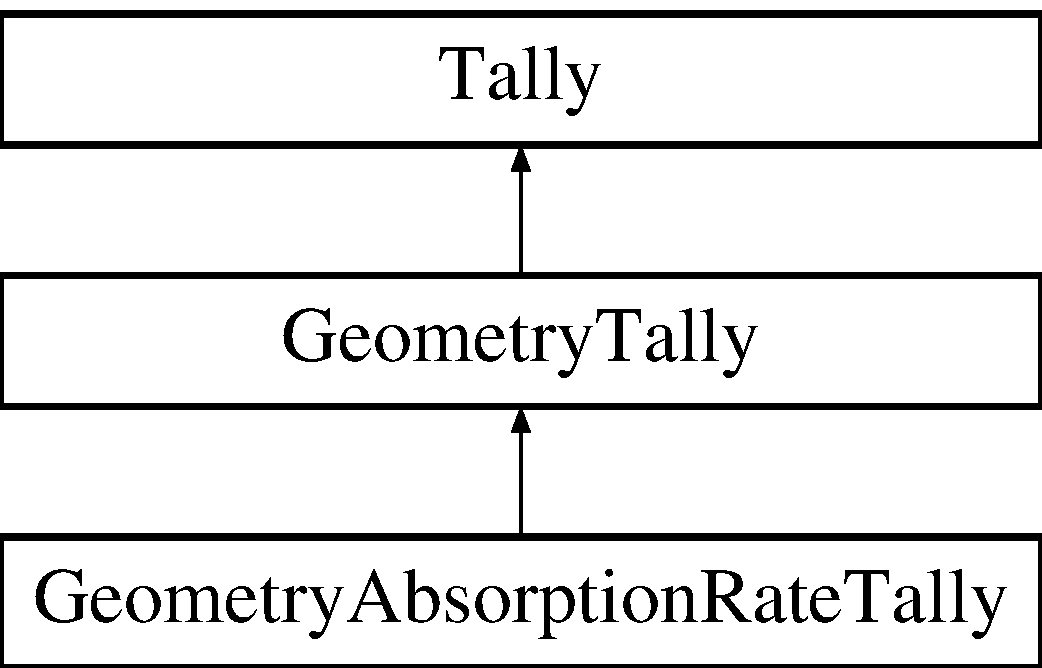
\includegraphics[height=3.000000cm]{classGeometryAbsorptionRateTally}
\end{center}
\end{figure}
\subsection*{Public Member Functions}
\begin{DoxyCompactItemize}
\item 
\hyperlink{classGeometryAbsorptionRateTally_ae5cc5e22df7445ae8ae9248dc768eb99}{Geometry\-Absorption\-Rate\-Tally} (\hyperlink{classGeometry}{Geometry} $\ast$geometry, const char $\ast$tally\-\_\-name=(char $\ast$)\char`\"{}\char`\"{})
\begin{DoxyCompactList}\small\item\em \hyperlink{classGeometryAbsorptionRateTally}{Geometry\-Absorption\-Rate\-Tally} constructor calls the \hyperlink{classGeometryTally}{Geometry\-Tally} constructor and \hyperlink{classTally}{Tally} constructors and sets the tally type to A\-B\-S\-O\-R\-P\-T\-I\-O\-N\-\_\-\-R\-A\-T\-E. \end{DoxyCompactList}\item 
void \hyperlink{classGeometryAbsorptionRateTally_a51490d9c5ee4a9d0447b6722a65fef1a}{tally} (\hyperlink{structneutron}{neutron} $\ast$\hyperlink{structneutron}{neutron})
\begin{DoxyCompactList}\small\item\em \hyperlink{classTally}{Tally} the region absorption rate by incrementing the tally by $ \frac{\Sigma_a}{\Sigma_t} $ at the neutron's energy. \end{DoxyCompactList}\end{DoxyCompactItemize}
\subsection*{Additional Inherited Members}


\subsection{Detailed Description}
A class for tallying the absorption within the geometry. 

\subsection{Constructor \& Destructor Documentation}
\hypertarget{classGeometryAbsorptionRateTally_ae5cc5e22df7445ae8ae9248dc768eb99}{\index{Geometry\-Absorption\-Rate\-Tally@{Geometry\-Absorption\-Rate\-Tally}!Geometry\-Absorption\-Rate\-Tally@{Geometry\-Absorption\-Rate\-Tally}}
\index{Geometry\-Absorption\-Rate\-Tally@{Geometry\-Absorption\-Rate\-Tally}!GeometryAbsorptionRateTally@{Geometry\-Absorption\-Rate\-Tally}}
\subsubsection[{Geometry\-Absorption\-Rate\-Tally}]{\setlength{\rightskip}{0pt plus 5cm}Geometry\-Absorption\-Rate\-Tally\-::\-Geometry\-Absorption\-Rate\-Tally (
\begin{DoxyParamCaption}
\item[{{\bf Geometry} $\ast$}]{geometry, }
\item[{const char $\ast$}]{tally\-\_\-name = {\ttfamily (char$\ast$)\char`\"{}\char`\"{}}}
\end{DoxyParamCaption}
)\hspace{0.3cm}{\ttfamily [inline]}}}\label{classGeometryAbsorptionRateTally_ae5cc5e22df7445ae8ae9248dc768eb99}


\hyperlink{classGeometryAbsorptionRateTally}{Geometry\-Absorption\-Rate\-Tally} constructor calls the \hyperlink{classGeometryTally}{Geometry\-Tally} constructor and \hyperlink{classTally}{Tally} constructors and sets the tally type to A\-B\-S\-O\-R\-P\-T\-I\-O\-N\-\_\-\-R\-A\-T\-E. 


\begin{DoxyParams}{Parameters}
{\em geometry} & a pointer to the geometry within which to tally \\
\hline
{\em tally\-\_\-name} & a character array for the tally name (optional) \\
\hline
\end{DoxyParams}


\subsection{Member Function Documentation}
\hypertarget{classGeometryAbsorptionRateTally_a51490d9c5ee4a9d0447b6722a65fef1a}{\index{Geometry\-Absorption\-Rate\-Tally@{Geometry\-Absorption\-Rate\-Tally}!tally@{tally}}
\index{tally@{tally}!GeometryAbsorptionRateTally@{Geometry\-Absorption\-Rate\-Tally}}
\subsubsection[{tally}]{\setlength{\rightskip}{0pt plus 5cm}void Geometry\-Absorption\-Rate\-Tally\-::tally (
\begin{DoxyParamCaption}
\item[{{\bf neutron} $\ast$}]{neutron}
\end{DoxyParamCaption}
)\hspace{0.3cm}{\ttfamily [virtual]}}}\label{classGeometryAbsorptionRateTally_a51490d9c5ee4a9d0447b6722a65fef1a}


\hyperlink{classTally}{Tally} the region absorption rate by incrementing the tally by $ \frac{\Sigma_a}{\Sigma_t} $ at the neutron's energy. 


\begin{DoxyParams}{Parameters}
{\em neutron} & the neutron of interest \\
\hline
\end{DoxyParams}


Implements \hyperlink{classGeometryTally_a3f79423e0c1e1eb87109c6937bdfa5c8}{Geometry\-Tally}.



The documentation for this class was generated from the following files\-:\begin{DoxyCompactItemize}
\item 
pinspec/src/\hyperlink{Tally_8h}{Tally.\-h}\item 
pinspec/src/Tally.\-cpp\end{DoxyCompactItemize}

\hypertarget{classGeometryCaptureRateTally}{\section{Geometry\-Capture\-Rate\-Tally Class Reference}
\label{classGeometryCaptureRateTally}\index{Geometry\-Capture\-Rate\-Tally@{Geometry\-Capture\-Rate\-Tally}}
}


A class for tallying the capture rate within the geometry.  




{\ttfamily \#include \char`\"{}pinspec/src/\-Tally.\-h\char`\"{}}

Inheritance diagram for Geometry\-Capture\-Rate\-Tally\-:\begin{figure}[H]
\begin{center}
\leavevmode
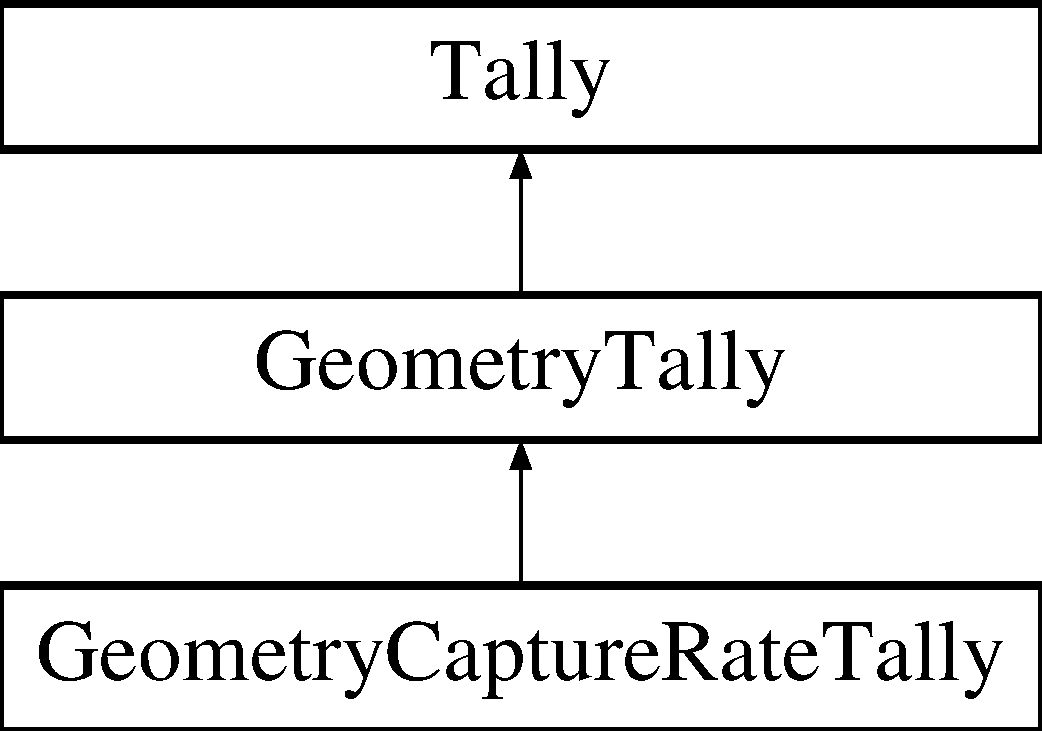
\includegraphics[height=3.000000cm]{classGeometryCaptureRateTally}
\end{center}
\end{figure}
\subsection*{Public Member Functions}
\begin{DoxyCompactItemize}
\item 
\hyperlink{classGeometryCaptureRateTally_a72f1cd00b35302766fbe074c00d4403c}{Geometry\-Capture\-Rate\-Tally} (\hyperlink{classGeometry}{Geometry} $\ast$geometry, const char $\ast$tally\-\_\-name=(char $\ast$)\char`\"{}\char`\"{})
\begin{DoxyCompactList}\small\item\em \hyperlink{classGeometryCaptureRateTally}{Geometry\-Capture\-Rate\-Tally} constructor calls the \hyperlink{classGeometryTally}{Geometry\-Tally} constructor and \hyperlink{classTally}{Tally} constructors and sets the tally type to C\-A\-P\-T\-U\-R\-E\-\_\-\-R\-A\-T\-E. \end{DoxyCompactList}\item 
void \hyperlink{classGeometryCaptureRateTally_a18b5cb68008c52ab416ee7f5b73ac2a5}{tally} (\hyperlink{structneutron}{neutron} $\ast$\hyperlink{structneutron}{neutron})
\begin{DoxyCompactList}\small\item\em \hyperlink{classTally}{Tally} the geometry capture rate by incrementing the tally by $ \frac{\Sigma_c}{\Sigma_t} $ at the neutron's energy. \end{DoxyCompactList}\end{DoxyCompactItemize}
\subsection*{Additional Inherited Members}


\subsection{Detailed Description}
A class for tallying the capture rate within the geometry. 

\subsection{Constructor \& Destructor Documentation}
\hypertarget{classGeometryCaptureRateTally_a72f1cd00b35302766fbe074c00d4403c}{\index{Geometry\-Capture\-Rate\-Tally@{Geometry\-Capture\-Rate\-Tally}!Geometry\-Capture\-Rate\-Tally@{Geometry\-Capture\-Rate\-Tally}}
\index{Geometry\-Capture\-Rate\-Tally@{Geometry\-Capture\-Rate\-Tally}!GeometryCaptureRateTally@{Geometry\-Capture\-Rate\-Tally}}
\subsubsection[{Geometry\-Capture\-Rate\-Tally}]{\setlength{\rightskip}{0pt plus 5cm}Geometry\-Capture\-Rate\-Tally\-::\-Geometry\-Capture\-Rate\-Tally (
\begin{DoxyParamCaption}
\item[{{\bf Geometry} $\ast$}]{geometry, }
\item[{const char $\ast$}]{tally\-\_\-name = {\ttfamily (char$\ast$)\char`\"{}\char`\"{}}}
\end{DoxyParamCaption}
)\hspace{0.3cm}{\ttfamily [inline]}}}\label{classGeometryCaptureRateTally_a72f1cd00b35302766fbe074c00d4403c}


\hyperlink{classGeometryCaptureRateTally}{Geometry\-Capture\-Rate\-Tally} constructor calls the \hyperlink{classGeometryTally}{Geometry\-Tally} constructor and \hyperlink{classTally}{Tally} constructors and sets the tally type to C\-A\-P\-T\-U\-R\-E\-\_\-\-R\-A\-T\-E. 


\begin{DoxyParams}{Parameters}
{\em geometry} & a pointer to the geometry within which to tally \\
\hline
{\em tally\-\_\-name} & a character array for the tally name (optional) \\
\hline
\end{DoxyParams}


\subsection{Member Function Documentation}
\hypertarget{classGeometryCaptureRateTally_a18b5cb68008c52ab416ee7f5b73ac2a5}{\index{Geometry\-Capture\-Rate\-Tally@{Geometry\-Capture\-Rate\-Tally}!tally@{tally}}
\index{tally@{tally}!GeometryCaptureRateTally@{Geometry\-Capture\-Rate\-Tally}}
\subsubsection[{tally}]{\setlength{\rightskip}{0pt plus 5cm}void Geometry\-Capture\-Rate\-Tally\-::tally (
\begin{DoxyParamCaption}
\item[{{\bf neutron} $\ast$}]{neutron}
\end{DoxyParamCaption}
)\hspace{0.3cm}{\ttfamily [virtual]}}}\label{classGeometryCaptureRateTally_a18b5cb68008c52ab416ee7f5b73ac2a5}


\hyperlink{classTally}{Tally} the geometry capture rate by incrementing the tally by $ \frac{\Sigma_c}{\Sigma_t} $ at the neutron's energy. 


\begin{DoxyParams}{Parameters}
{\em neutron} & the neutron of interest \\
\hline
\end{DoxyParams}


Implements \hyperlink{classGeometryTally_a3f79423e0c1e1eb87109c6937bdfa5c8}{Geometry\-Tally}.



The documentation for this class was generated from the following files\-:\begin{DoxyCompactItemize}
\item 
pinspec/src/\hyperlink{Tally_8h}{Tally.\-h}\item 
pinspec/src/Tally.\-cpp\end{DoxyCompactItemize}

\hypertarget{classGeometryCollisionRateTally}{\section{Geometry\-Collision\-Rate\-Tally Class Reference}
\label{classGeometryCollisionRateTally}\index{Geometry\-Collision\-Rate\-Tally@{Geometry\-Collision\-Rate\-Tally}}
}


A class for tallying the collision rate within the geometry.  




{\ttfamily \#include \char`\"{}pinspec/src/\-Tally.\-h\char`\"{}}

Inheritance diagram for Geometry\-Collision\-Rate\-Tally\-:\begin{figure}[H]
\begin{center}
\leavevmode
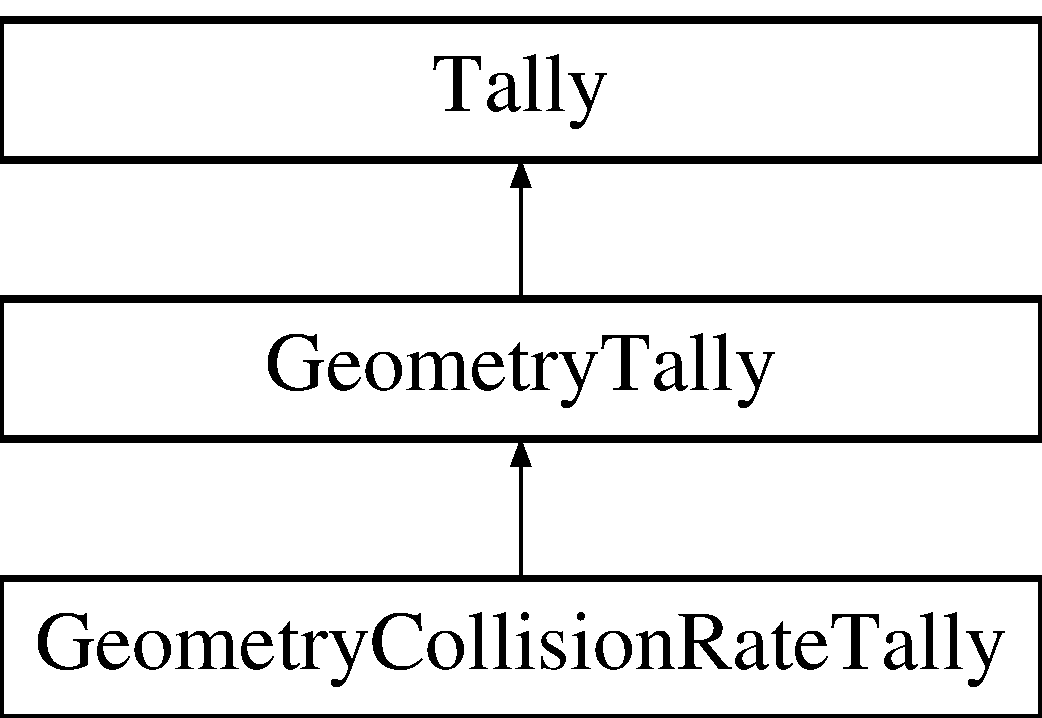
\includegraphics[height=3.000000cm]{classGeometryCollisionRateTally}
\end{center}
\end{figure}
\subsection*{Public Member Functions}
\begin{DoxyCompactItemize}
\item 
\hyperlink{classGeometryCollisionRateTally_a7227a1c5cf9e9490f52fc197e47e0bae}{Geometry\-Collision\-Rate\-Tally} (\hyperlink{classGeometry}{Geometry} $\ast$geometry, const char $\ast$tally\-\_\-name=(char $\ast$)\char`\"{}\char`\"{})
\begin{DoxyCompactList}\small\item\em \hyperlink{classGeometryCollisionRateTally}{Geometry\-Collision\-Rate\-Tally} constructor calls the \hyperlink{classGeometryTally}{Geometry\-Tally} constructor and \hyperlink{classTally}{Tally} constructors and sets the tally type to C\-O\-L\-L\-I\-S\-I\-O\-N\-\_\-\-R\-A\-T\-E. \end{DoxyCompactList}\item 
void \hyperlink{classGeometryCollisionRateTally_af0b0c1c09c8dbdc5453feb8366600dc0}{tally} (\hyperlink{structneutron}{neutron} $\ast$\hyperlink{structneutron}{neutron})
\begin{DoxyCompactList}\small\item\em \hyperlink{classTally}{Tally} the geometry collision rate by incrementing the tally by 1.\-0 at the neutron's energy. \end{DoxyCompactList}\end{DoxyCompactItemize}
\subsection*{Additional Inherited Members}


\subsection{Detailed Description}
A class for tallying the collision rate within the geometry. 

\subsection{Constructor \& Destructor Documentation}
\hypertarget{classGeometryCollisionRateTally_a7227a1c5cf9e9490f52fc197e47e0bae}{\index{Geometry\-Collision\-Rate\-Tally@{Geometry\-Collision\-Rate\-Tally}!Geometry\-Collision\-Rate\-Tally@{Geometry\-Collision\-Rate\-Tally}}
\index{Geometry\-Collision\-Rate\-Tally@{Geometry\-Collision\-Rate\-Tally}!GeometryCollisionRateTally@{Geometry\-Collision\-Rate\-Tally}}
\subsubsection[{Geometry\-Collision\-Rate\-Tally}]{\setlength{\rightskip}{0pt plus 5cm}Geometry\-Collision\-Rate\-Tally\-::\-Geometry\-Collision\-Rate\-Tally (
\begin{DoxyParamCaption}
\item[{{\bf Geometry} $\ast$}]{geometry, }
\item[{const char $\ast$}]{tally\-\_\-name = {\ttfamily (char$\ast$)\char`\"{}\char`\"{}}}
\end{DoxyParamCaption}
)\hspace{0.3cm}{\ttfamily [inline]}}}\label{classGeometryCollisionRateTally_a7227a1c5cf9e9490f52fc197e47e0bae}


\hyperlink{classGeometryCollisionRateTally}{Geometry\-Collision\-Rate\-Tally} constructor calls the \hyperlink{classGeometryTally}{Geometry\-Tally} constructor and \hyperlink{classTally}{Tally} constructors and sets the tally type to C\-O\-L\-L\-I\-S\-I\-O\-N\-\_\-\-R\-A\-T\-E. 


\begin{DoxyParams}{Parameters}
{\em geometry} & a pointer to the geometry within which to tally \\
\hline
{\em tally\-\_\-name} & a character array for the tally name (optional) \\
\hline
\end{DoxyParams}


\subsection{Member Function Documentation}
\hypertarget{classGeometryCollisionRateTally_af0b0c1c09c8dbdc5453feb8366600dc0}{\index{Geometry\-Collision\-Rate\-Tally@{Geometry\-Collision\-Rate\-Tally}!tally@{tally}}
\index{tally@{tally}!GeometryCollisionRateTally@{Geometry\-Collision\-Rate\-Tally}}
\subsubsection[{tally}]{\setlength{\rightskip}{0pt plus 5cm}void Geometry\-Collision\-Rate\-Tally\-::tally (
\begin{DoxyParamCaption}
\item[{{\bf neutron} $\ast$}]{neutron}
\end{DoxyParamCaption}
)\hspace{0.3cm}{\ttfamily [virtual]}}}\label{classGeometryCollisionRateTally_af0b0c1c09c8dbdc5453feb8366600dc0}


\hyperlink{classTally}{Tally} the geometry collision rate by incrementing the tally by 1.\-0 at the neutron's energy. 


\begin{DoxyParams}{Parameters}
{\em neutron} & the neutron of interest \\
\hline
\end{DoxyParams}


Implements \hyperlink{classGeometryTally_a3f79423e0c1e1eb87109c6937bdfa5c8}{Geometry\-Tally}.



The documentation for this class was generated from the following files\-:\begin{DoxyCompactItemize}
\item 
\hyperlink{Tally_8h}{Tally.\-h}\item 
Tally.\-cpp\end{DoxyCompactItemize}

\hypertarget{classGeometryDiffusionRateTally}{\section{Geometry\-Diffusion\-Rate\-Tally Class Reference}
\label{classGeometryDiffusionRateTally}\index{Geometry\-Diffusion\-Rate\-Tally@{Geometry\-Diffusion\-Rate\-Tally}}
}


A class for tallying the capture rate for an isotope.  




{\ttfamily \#include \char`\"{}pinspec/src/\-Tally.\-h\char`\"{}}

Inheritance diagram for Geometry\-Diffusion\-Rate\-Tally\-:\begin{figure}[H]
\begin{center}
\leavevmode
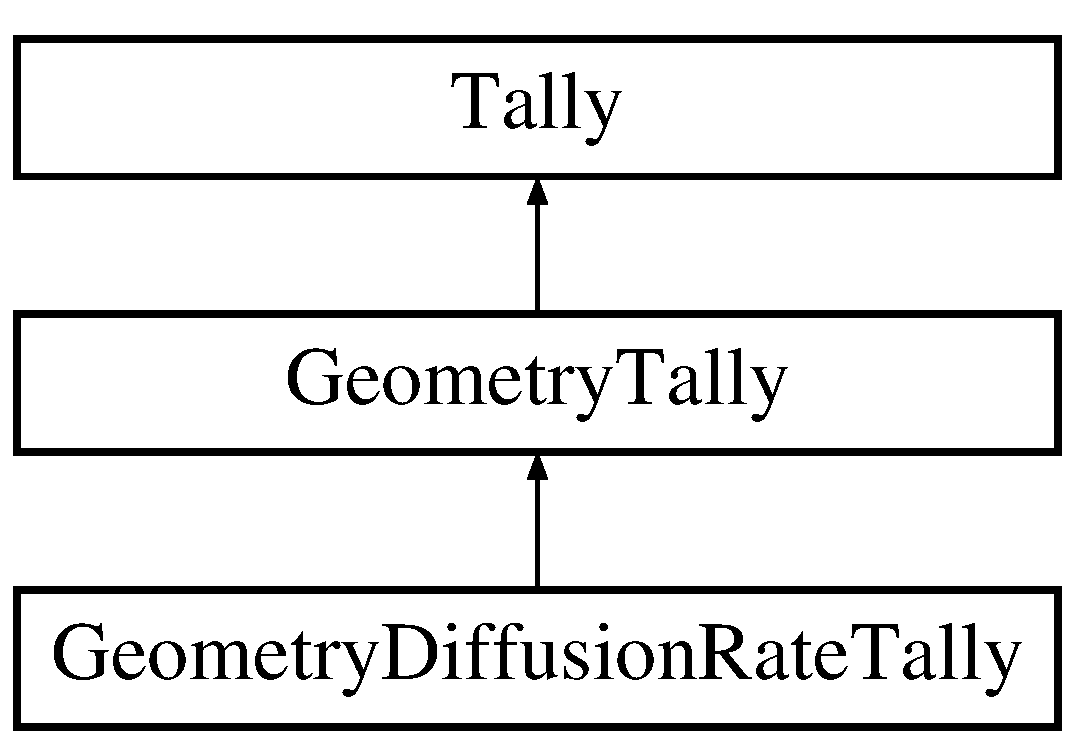
\includegraphics[height=3.000000cm]{classGeometryDiffusionRateTally}
\end{center}
\end{figure}
\subsection*{Public Member Functions}
\begin{DoxyCompactItemize}
\item 
\hyperlink{classGeometryDiffusionRateTally_ad7813cacc07a6833a25dfddba0ee7cf4}{Geometry\-Diffusion\-Rate\-Tally} (\hyperlink{classGeometry}{Geometry} $\ast$geometry, const char $\ast$tally\-\_\-name=(char $\ast$)\char`\"{}\char`\"{})
\begin{DoxyCompactList}\small\item\em \hyperlink{classGeometryDiffusionRateTally}{Geometry\-Diffusion\-Rate\-Tally} constructor calls the \hyperlink{classGeometryTally}{Geometry\-Tally} constructor and \hyperlink{classTally}{Tally} constructors and sets the tally type to D\-I\-F\-F\-U\-S\-I\-O\-N\-\_\-\-R\-A\-T\-E. \end{DoxyCompactList}\item 
void \hyperlink{classGeometryDiffusionRateTally_aab31c320a689adb46c888bd68df49ad4}{tally} (\hyperlink{structneutron}{neutron} $\ast$\hyperlink{structneutron}{neutron})
\begin{DoxyCompactList}\small\item\em \hyperlink{classTally}{Tally} the geometry diffusion rate by incrementing the tally by $ \frac{\frac{1}{3\Sigma_tr}}{\Sigma_t} $ at the neutron's energy. \end{DoxyCompactList}\end{DoxyCompactItemize}
\subsection*{Additional Inherited Members}


\subsection{Detailed Description}
A class for tallying the capture rate for an isotope. 

\subsection{Constructor \& Destructor Documentation}
\hypertarget{classGeometryDiffusionRateTally_ad7813cacc07a6833a25dfddba0ee7cf4}{\index{Geometry\-Diffusion\-Rate\-Tally@{Geometry\-Diffusion\-Rate\-Tally}!Geometry\-Diffusion\-Rate\-Tally@{Geometry\-Diffusion\-Rate\-Tally}}
\index{Geometry\-Diffusion\-Rate\-Tally@{Geometry\-Diffusion\-Rate\-Tally}!GeometryDiffusionRateTally@{Geometry\-Diffusion\-Rate\-Tally}}
\subsubsection[{Geometry\-Diffusion\-Rate\-Tally}]{\setlength{\rightskip}{0pt plus 5cm}Geometry\-Diffusion\-Rate\-Tally\-::\-Geometry\-Diffusion\-Rate\-Tally (
\begin{DoxyParamCaption}
\item[{{\bf Geometry} $\ast$}]{geometry, }
\item[{const char $\ast$}]{tally\-\_\-name = {\ttfamily (char$\ast$)\char`\"{}\char`\"{}}}
\end{DoxyParamCaption}
)\hspace{0.3cm}{\ttfamily [inline]}}}\label{classGeometryDiffusionRateTally_ad7813cacc07a6833a25dfddba0ee7cf4}


\hyperlink{classGeometryDiffusionRateTally}{Geometry\-Diffusion\-Rate\-Tally} constructor calls the \hyperlink{classGeometryTally}{Geometry\-Tally} constructor and \hyperlink{classTally}{Tally} constructors and sets the tally type to D\-I\-F\-F\-U\-S\-I\-O\-N\-\_\-\-R\-A\-T\-E. 


\begin{DoxyParams}{Parameters}
{\em geometry} & a pointer to the geometry within which to tally \\
\hline
{\em tally\-\_\-name} & a character array for the tally name (optional) \\
\hline
\end{DoxyParams}


\subsection{Member Function Documentation}
\hypertarget{classGeometryDiffusionRateTally_aab31c320a689adb46c888bd68df49ad4}{\index{Geometry\-Diffusion\-Rate\-Tally@{Geometry\-Diffusion\-Rate\-Tally}!tally@{tally}}
\index{tally@{tally}!GeometryDiffusionRateTally@{Geometry\-Diffusion\-Rate\-Tally}}
\subsubsection[{tally}]{\setlength{\rightskip}{0pt plus 5cm}void Geometry\-Diffusion\-Rate\-Tally\-::tally (
\begin{DoxyParamCaption}
\item[{{\bf neutron} $\ast$}]{neutron}
\end{DoxyParamCaption}
)\hspace{0.3cm}{\ttfamily [virtual]}}}\label{classGeometryDiffusionRateTally_aab31c320a689adb46c888bd68df49ad4}


\hyperlink{classTally}{Tally} the geometry diffusion rate by incrementing the tally by $ \frac{\frac{1}{3\Sigma_tr}}{\Sigma_t} $ at the neutron's energy. 


\begin{DoxyParams}{Parameters}
{\em neutron} & the neutron of interest \\
\hline
\end{DoxyParams}


Implements \hyperlink{classGeometryTally_a3f79423e0c1e1eb87109c6937bdfa5c8}{Geometry\-Tally}.



The documentation for this class was generated from the following files\-:\begin{DoxyCompactItemize}
\item 
\hyperlink{Tally_8h}{Tally.\-h}\item 
Tally.\-cpp\end{DoxyCompactItemize}

\hypertarget{classGeometryElasticRateTally}{\section{Geometry\-Elastic\-Rate\-Tally Class Reference}
\label{classGeometryElasticRateTally}\index{Geometry\-Elastic\-Rate\-Tally@{Geometry\-Elastic\-Rate\-Tally}}
}


A class for tallying the elastic scattering rate within the geometry.  




{\ttfamily \#include \char`\"{}pinspec/src/\-Tally.\-h\char`\"{}}

Inheritance diagram for Geometry\-Elastic\-Rate\-Tally\-:\begin{figure}[H]
\begin{center}
\leavevmode
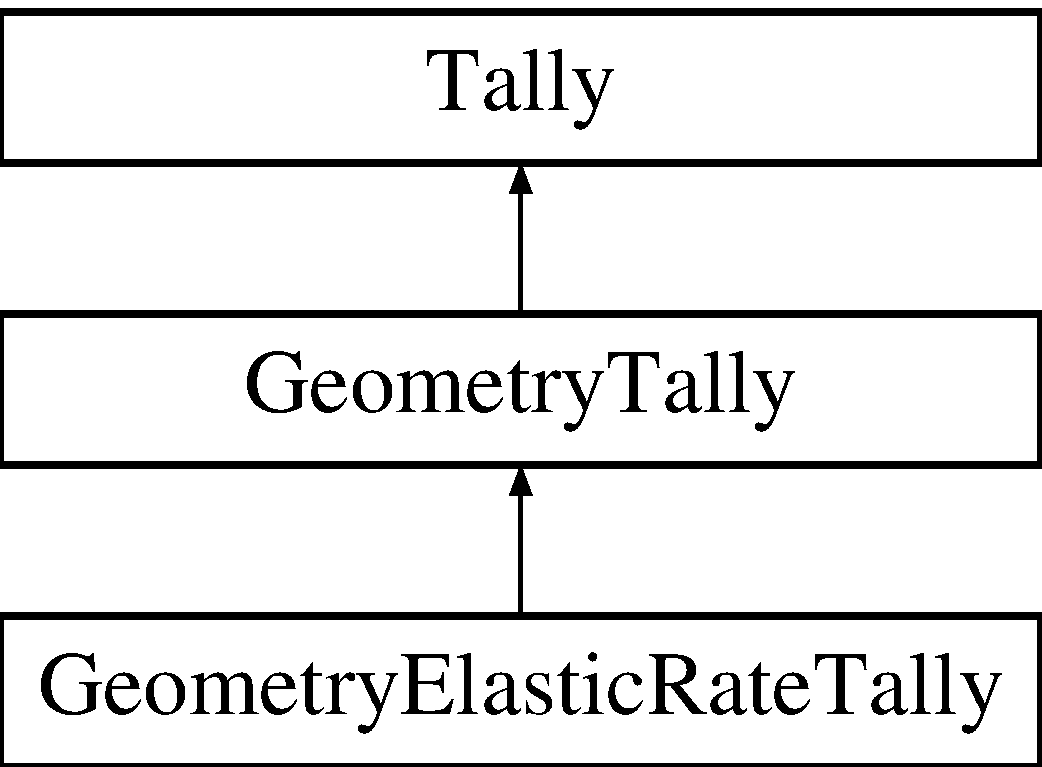
\includegraphics[height=3.000000cm]{classGeometryElasticRateTally}
\end{center}
\end{figure}
\subsection*{Public Member Functions}
\begin{DoxyCompactItemize}
\item 
\hyperlink{classGeometryElasticRateTally_acae25bceffafeb18ab0552dcca9b11df}{Geometry\-Elastic\-Rate\-Tally} (\hyperlink{classGeometry}{Geometry} $\ast$geometry, const char $\ast$tally\-\_\-name=(char $\ast$)\char`\"{}\char`\"{})
\begin{DoxyCompactList}\small\item\em \hyperlink{classGeometryElasticRateTally}{Geometry\-Elastic\-Rate\-Tally} constructor calls the \hyperlink{classGeometryTally}{Geometry\-Tally} constructor and \hyperlink{classTally}{Tally} constructors and sets the tally type to E\-L\-A\-S\-T\-I\-C\-\_\-\-R\-A\-T\-E. \end{DoxyCompactList}\item 
void \hyperlink{classGeometryElasticRateTally_a7bf2a8bc3afbc47354bad45159237ec3}{tally} (\hyperlink{structneutron}{neutron} $\ast$\hyperlink{structneutron}{neutron})
\begin{DoxyCompactList}\small\item\em \hyperlink{classTally}{Tally} the geometry elastic scattering rate by incrementing the tally by $ \frac{\Sigma_s}{\Sigma_t} $ at the neutron's energy. \end{DoxyCompactList}\end{DoxyCompactItemize}
\subsection*{Additional Inherited Members}


\subsection{Detailed Description}
A class for tallying the elastic scattering rate within the geometry. 

\subsection{Constructor \& Destructor Documentation}
\hypertarget{classGeometryElasticRateTally_acae25bceffafeb18ab0552dcca9b11df}{\index{Geometry\-Elastic\-Rate\-Tally@{Geometry\-Elastic\-Rate\-Tally}!Geometry\-Elastic\-Rate\-Tally@{Geometry\-Elastic\-Rate\-Tally}}
\index{Geometry\-Elastic\-Rate\-Tally@{Geometry\-Elastic\-Rate\-Tally}!GeometryElasticRateTally@{Geometry\-Elastic\-Rate\-Tally}}
\subsubsection[{Geometry\-Elastic\-Rate\-Tally}]{\setlength{\rightskip}{0pt plus 5cm}Geometry\-Elastic\-Rate\-Tally\-::\-Geometry\-Elastic\-Rate\-Tally (
\begin{DoxyParamCaption}
\item[{{\bf Geometry} $\ast$}]{geometry, }
\item[{const char $\ast$}]{tally\-\_\-name = {\ttfamily (char$\ast$)\char`\"{}\char`\"{}}}
\end{DoxyParamCaption}
)\hspace{0.3cm}{\ttfamily [inline]}}}\label{classGeometryElasticRateTally_acae25bceffafeb18ab0552dcca9b11df}


\hyperlink{classGeometryElasticRateTally}{Geometry\-Elastic\-Rate\-Tally} constructor calls the \hyperlink{classGeometryTally}{Geometry\-Tally} constructor and \hyperlink{classTally}{Tally} constructors and sets the tally type to E\-L\-A\-S\-T\-I\-C\-\_\-\-R\-A\-T\-E. 


\begin{DoxyParams}{Parameters}
{\em geometry} & a pointer to the geometry within which to tally \\
\hline
{\em tally\-\_\-name} & a character array for the tally name (optional) \\
\hline
\end{DoxyParams}


\subsection{Member Function Documentation}
\hypertarget{classGeometryElasticRateTally_a7bf2a8bc3afbc47354bad45159237ec3}{\index{Geometry\-Elastic\-Rate\-Tally@{Geometry\-Elastic\-Rate\-Tally}!tally@{tally}}
\index{tally@{tally}!GeometryElasticRateTally@{Geometry\-Elastic\-Rate\-Tally}}
\subsubsection[{tally}]{\setlength{\rightskip}{0pt plus 5cm}void Geometry\-Elastic\-Rate\-Tally\-::tally (
\begin{DoxyParamCaption}
\item[{{\bf neutron} $\ast$}]{neutron}
\end{DoxyParamCaption}
)\hspace{0.3cm}{\ttfamily [virtual]}}}\label{classGeometryElasticRateTally_a7bf2a8bc3afbc47354bad45159237ec3}


\hyperlink{classTally}{Tally} the geometry elastic scattering rate by incrementing the tally by $ \frac{\Sigma_s}{\Sigma_t} $ at the neutron's energy. 


\begin{DoxyParams}{Parameters}
{\em neutron} & the neutron of interest \\
\hline
\end{DoxyParams}


Implements \hyperlink{classGeometryTally_a3f79423e0c1e1eb87109c6937bdfa5c8}{Geometry\-Tally}.



The documentation for this class was generated from the following files\-:\begin{DoxyCompactItemize}
\item 
\hyperlink{Tally_8h}{Tally.\-h}\item 
Tally.\-cpp\end{DoxyCompactItemize}

\hypertarget{classGeometryFissionRateTally}{\section{Geometry\-Fission\-Rate\-Tally Class Reference}
\label{classGeometryFissionRateTally}\index{Geometry\-Fission\-Rate\-Tally@{Geometry\-Fission\-Rate\-Tally}}
}


A class for tallying the capture rate for an isotope.  




{\ttfamily \#include \char`\"{}pinspec/src/\-Tally.\-h\char`\"{}}

Inheritance diagram for Geometry\-Fission\-Rate\-Tally\-:\begin{figure}[H]
\begin{center}
\leavevmode
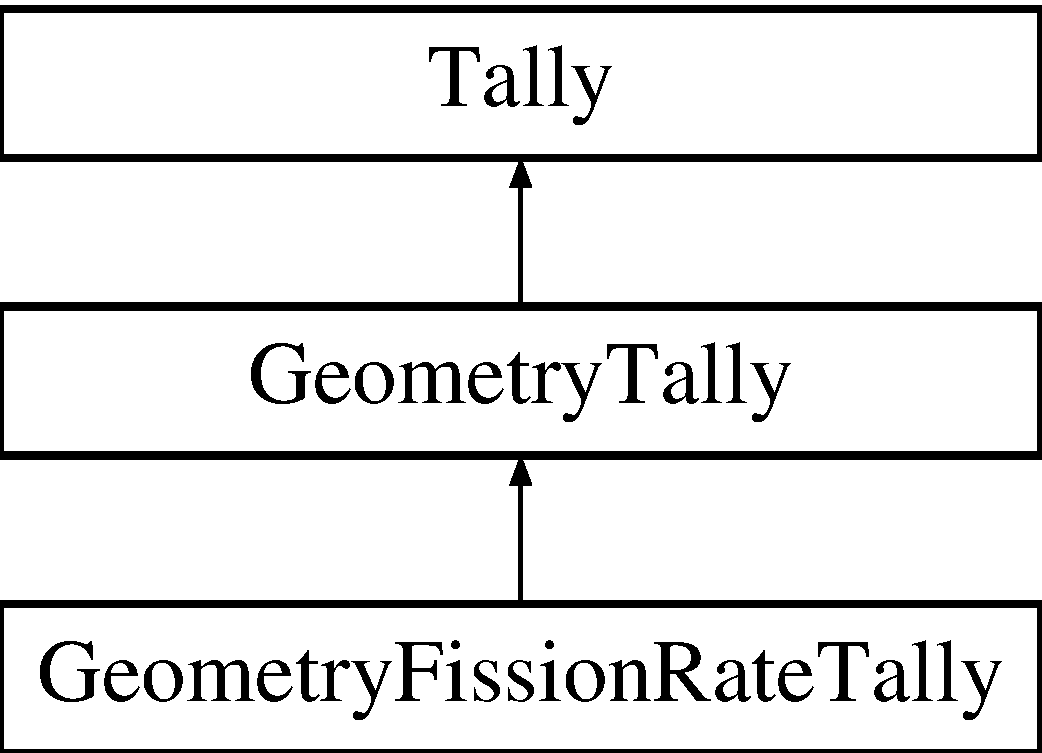
\includegraphics[height=3.000000cm]{classGeometryFissionRateTally}
\end{center}
\end{figure}
\subsection*{Public Member Functions}
\begin{DoxyCompactItemize}
\item 
\hyperlink{classGeometryFissionRateTally_a041d7971d78dd0c45287242720e33d32}{Geometry\-Fission\-Rate\-Tally} (\hyperlink{classGeometry}{Geometry} $\ast$geometry, const char $\ast$tally\-\_\-name=(char $\ast$)\char`\"{}\char`\"{})
\begin{DoxyCompactList}\small\item\em \hyperlink{classGeometryFissionRateTally}{Geometry\-Fission\-Rate\-Tally} constructor calls the \hyperlink{classGeometryTally}{Geometry\-Tally} constructor and \hyperlink{classTally}{Tally} constructors and sets the tally type to F\-I\-S\-S\-I\-O\-N\-\_\-\-R\-A\-T\-E. \end{DoxyCompactList}\item 
void \hyperlink{classGeometryFissionRateTally_aabf84c492a081ac3fb86993be3896a62}{tally} (\hyperlink{structneutron}{neutron} $\ast$\hyperlink{structneutron}{neutron})
\begin{DoxyCompactList}\small\item\em \hyperlink{classTally}{Tally} the geometry fission rate by incrementing the tally by $ \frac{\Sigma_f}{\Sigma_t} $ at the neutron's energy. \end{DoxyCompactList}\end{DoxyCompactItemize}
\subsection*{Additional Inherited Members}


\subsection{Detailed Description}
A class for tallying the capture rate for an isotope. 

\subsection{Constructor \& Destructor Documentation}
\hypertarget{classGeometryFissionRateTally_a041d7971d78dd0c45287242720e33d32}{\index{Geometry\-Fission\-Rate\-Tally@{Geometry\-Fission\-Rate\-Tally}!Geometry\-Fission\-Rate\-Tally@{Geometry\-Fission\-Rate\-Tally}}
\index{Geometry\-Fission\-Rate\-Tally@{Geometry\-Fission\-Rate\-Tally}!GeometryFissionRateTally@{Geometry\-Fission\-Rate\-Tally}}
\subsubsection[{Geometry\-Fission\-Rate\-Tally}]{\setlength{\rightskip}{0pt plus 5cm}Geometry\-Fission\-Rate\-Tally\-::\-Geometry\-Fission\-Rate\-Tally (
\begin{DoxyParamCaption}
\item[{{\bf Geometry} $\ast$}]{geometry, }
\item[{const char $\ast$}]{tally\-\_\-name = {\ttfamily (char$\ast$)\char`\"{}\char`\"{}}}
\end{DoxyParamCaption}
)\hspace{0.3cm}{\ttfamily [inline]}}}\label{classGeometryFissionRateTally_a041d7971d78dd0c45287242720e33d32}


\hyperlink{classGeometryFissionRateTally}{Geometry\-Fission\-Rate\-Tally} constructor calls the \hyperlink{classGeometryTally}{Geometry\-Tally} constructor and \hyperlink{classTally}{Tally} constructors and sets the tally type to F\-I\-S\-S\-I\-O\-N\-\_\-\-R\-A\-T\-E. 


\begin{DoxyParams}{Parameters}
{\em geometry} & a pointer to the geometry within which to tally \\
\hline
{\em tally\-\_\-name} & a character array for the tally name (optional) \\
\hline
\end{DoxyParams}


\subsection{Member Function Documentation}
\hypertarget{classGeometryFissionRateTally_aabf84c492a081ac3fb86993be3896a62}{\index{Geometry\-Fission\-Rate\-Tally@{Geometry\-Fission\-Rate\-Tally}!tally@{tally}}
\index{tally@{tally}!GeometryFissionRateTally@{Geometry\-Fission\-Rate\-Tally}}
\subsubsection[{tally}]{\setlength{\rightskip}{0pt plus 5cm}void Geometry\-Fission\-Rate\-Tally\-::tally (
\begin{DoxyParamCaption}
\item[{{\bf neutron} $\ast$}]{neutron}
\end{DoxyParamCaption}
)\hspace{0.3cm}{\ttfamily [virtual]}}}\label{classGeometryFissionRateTally_aabf84c492a081ac3fb86993be3896a62}


\hyperlink{classTally}{Tally} the geometry fission rate by incrementing the tally by $ \frac{\Sigma_f}{\Sigma_t} $ at the neutron's energy. 


\begin{DoxyParams}{Parameters}
{\em neutron} & the neutron of interest \\
\hline
\end{DoxyParams}


Implements \hyperlink{classGeometryTally_a3f79423e0c1e1eb87109c6937bdfa5c8}{Geometry\-Tally}.



The documentation for this class was generated from the following files\-:\begin{DoxyCompactItemize}
\item 
pinspec/src/\hyperlink{Tally_8h}{Tally.\-h}\item 
pinspec/src/Tally.\-cpp\end{DoxyCompactItemize}

\hypertarget{classGeometryFluxTally}{\section{Geometry\-Flux\-Tally Class Reference}
\label{classGeometryFluxTally}\index{Geometry\-Flux\-Tally@{Geometry\-Flux\-Tally}}
}


A class for tallying the flux for the geometry.  




{\ttfamily \#include \char`\"{}pinspec/src/\-Tally.\-h\char`\"{}}

Inheritance diagram for Geometry\-Flux\-Tally\-:\begin{figure}[H]
\begin{center}
\leavevmode
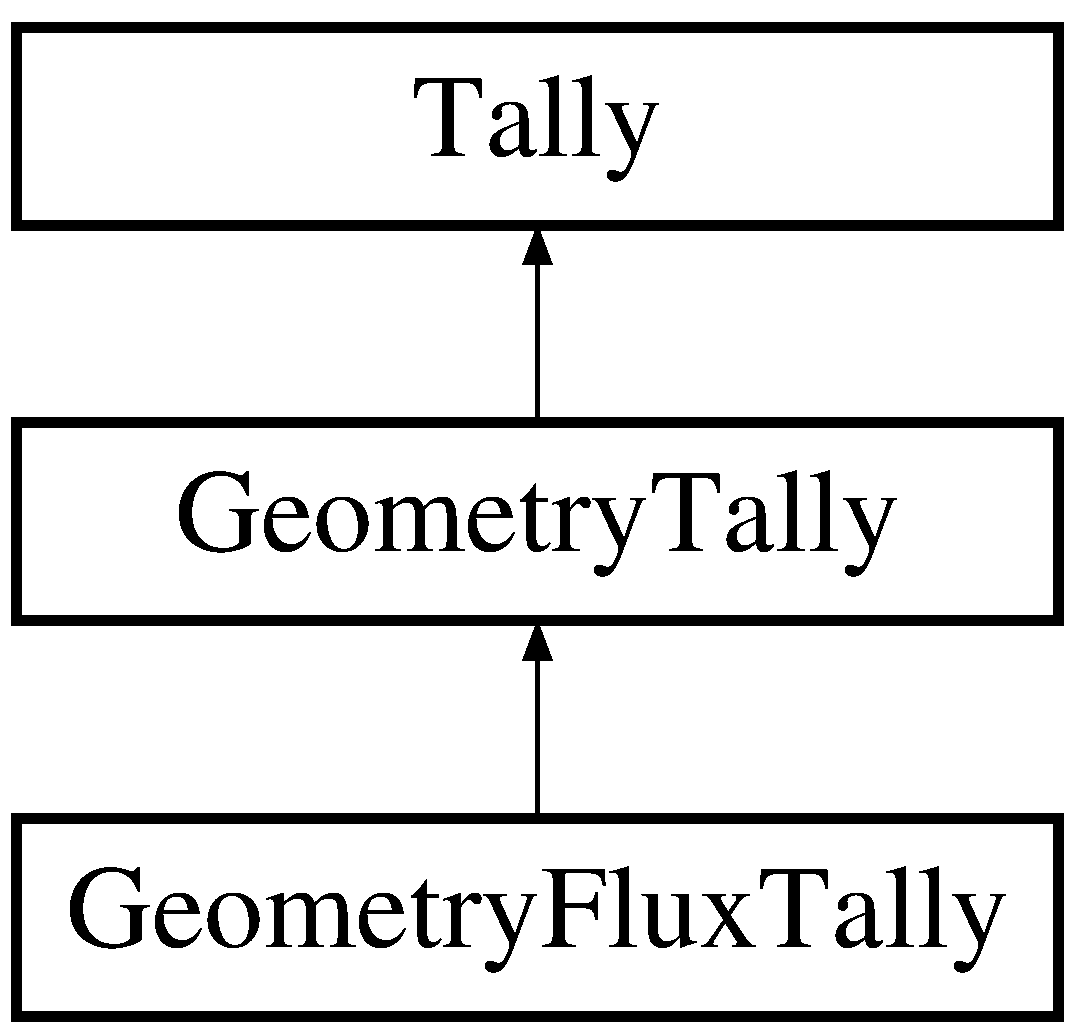
\includegraphics[height=3.000000cm]{classGeometryFluxTally}
\end{center}
\end{figure}
\subsection*{Public Member Functions}
\begin{DoxyCompactItemize}
\item 
\hyperlink{classGeometryFluxTally_afe633b1d646dfe7bbf3232cb49095356}{Geometry\-Flux\-Tally} (\hyperlink{classGeometry}{Geometry} $\ast$geometry, const char $\ast$tally\-\_\-name=(char $\ast$)\char`\"{}\char`\"{})
\begin{DoxyCompactList}\small\item\em \hyperlink{classGeometryFluxTally}{Geometry\-Flux\-Tally} constructor calls the \hyperlink{classGeometryTally}{Geometry\-Tally} constructor and \hyperlink{classTally}{Tally} constructors and sets the tally type to F\-L\-U\-X. \end{DoxyCompactList}\item 
void \hyperlink{classGeometryFluxTally_a2c7d83a4577cff56a1cecf8a339db547}{tally} (\hyperlink{structneutron}{neutron} $\ast$\hyperlink{structneutron}{neutron})
\begin{DoxyCompactList}\small\item\em \hyperlink{classTally}{Tally} the geomety flux by incrementing the tally by $ \frac{1}{\Sigma_t} $ at the neutron's energy. \end{DoxyCompactList}\end{DoxyCompactItemize}
\subsection*{Additional Inherited Members}


\subsection{Detailed Description}
A class for tallying the flux for the geometry. 

\subsection{Constructor \& Destructor Documentation}
\hypertarget{classGeometryFluxTally_afe633b1d646dfe7bbf3232cb49095356}{\index{Geometry\-Flux\-Tally@{Geometry\-Flux\-Tally}!Geometry\-Flux\-Tally@{Geometry\-Flux\-Tally}}
\index{Geometry\-Flux\-Tally@{Geometry\-Flux\-Tally}!GeometryFluxTally@{Geometry\-Flux\-Tally}}
\subsubsection[{Geometry\-Flux\-Tally}]{\setlength{\rightskip}{0pt plus 5cm}Geometry\-Flux\-Tally\-::\-Geometry\-Flux\-Tally (
\begin{DoxyParamCaption}
\item[{{\bf Geometry} $\ast$}]{geometry, }
\item[{const char $\ast$}]{tally\-\_\-name = {\ttfamily (char$\ast$)\char`\"{}\char`\"{}}}
\end{DoxyParamCaption}
)\hspace{0.3cm}{\ttfamily [inline]}}}\label{classGeometryFluxTally_afe633b1d646dfe7bbf3232cb49095356}


\hyperlink{classGeometryFluxTally}{Geometry\-Flux\-Tally} constructor calls the \hyperlink{classGeometryTally}{Geometry\-Tally} constructor and \hyperlink{classTally}{Tally} constructors and sets the tally type to F\-L\-U\-X. 


\begin{DoxyParams}{Parameters}
{\em geometry} & a pointer to the geometry within which to tally \\
\hline
{\em tally\-\_\-name} & a character array for the tally name (optional) \\
\hline
\end{DoxyParams}


\subsection{Member Function Documentation}
\hypertarget{classGeometryFluxTally_a2c7d83a4577cff56a1cecf8a339db547}{\index{Geometry\-Flux\-Tally@{Geometry\-Flux\-Tally}!tally@{tally}}
\index{tally@{tally}!GeometryFluxTally@{Geometry\-Flux\-Tally}}
\subsubsection[{tally}]{\setlength{\rightskip}{0pt plus 5cm}void Geometry\-Flux\-Tally\-::tally (
\begin{DoxyParamCaption}
\item[{{\bf neutron} $\ast$}]{neutron}
\end{DoxyParamCaption}
)\hspace{0.3cm}{\ttfamily [virtual]}}}\label{classGeometryFluxTally_a2c7d83a4577cff56a1cecf8a339db547}


\hyperlink{classTally}{Tally} the geomety flux by incrementing the tally by $ \frac{1}{\Sigma_t} $ at the neutron's energy. 


\begin{DoxyParams}{Parameters}
{\em neutron} & the neutron of interest \\
\hline
\end{DoxyParams}


Implements \hyperlink{classGeometryTally_a3f79423e0c1e1eb87109c6937bdfa5c8}{Geometry\-Tally}.



The documentation for this class was generated from the following files\-:\begin{DoxyCompactItemize}
\item 
\hyperlink{Tally_8h}{Tally.\-h}\item 
Tally.\-cpp\end{DoxyCompactItemize}

\hypertarget{classGeometryInterCollisionTimeTally}{\section{Geometry\-Inter\-Collision\-Time\-Tally Class Reference}
\label{classGeometryInterCollisionTimeTally}\index{Geometry\-Inter\-Collision\-Time\-Tally@{Geometry\-Inter\-Collision\-Time\-Tally}}
}


A class for tallying the time between collisions for the geometry.  




{\ttfamily \#include \char`\"{}pinspec/src/\-Tally.\-h\char`\"{}}

Inheritance diagram for Geometry\-Inter\-Collision\-Time\-Tally\-:\begin{figure}[H]
\begin{center}
\leavevmode
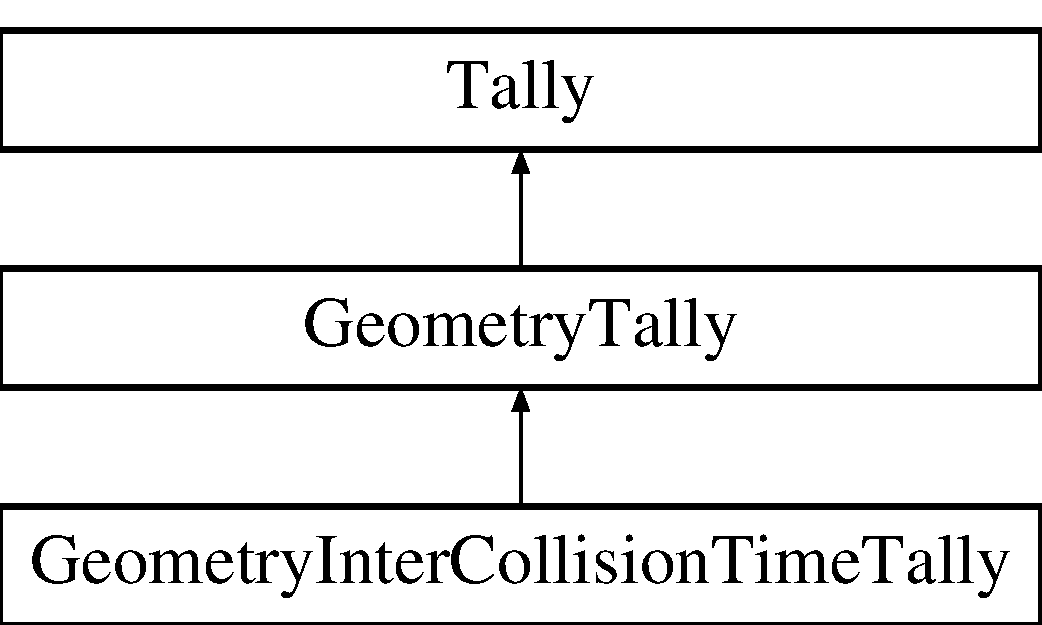
\includegraphics[height=3.000000cm]{classGeometryInterCollisionTimeTally}
\end{center}
\end{figure}
\subsection*{Public Member Functions}
\begin{DoxyCompactItemize}
\item 
\hyperlink{classGeometryInterCollisionTimeTally_abeda6d89eff389576d4f4b5e8a6b5987}{Geometry\-Inter\-Collision\-Time\-Tally} (\hyperlink{classGeometry}{Geometry} $\ast$geometry, const char $\ast$tally\-\_\-name=(char $\ast$)\char`\"{}\char`\"{})
\begin{DoxyCompactList}\small\item\em \hyperlink{classGeometryInterCollisionTimeTally}{Geometry\-Inter\-Collision\-Time\-Tally} constructor calls the \hyperlink{classGeometryTally}{Geometry\-Tally} constructor and \hyperlink{classTally}{Tally} constructors and sets the tally type to I\-N\-T\-E\-R\-C\-O\-L\-L\-I\-S\-I\-O\-N\-\_\-\-T\-I\-M\-E. \end{DoxyCompactList}\item 
void \hyperlink{classGeometryInterCollisionTimeTally_a8190817fa635809c6ae1bdadd9665ef8}{tally} (\hyperlink{structneutron}{neutron} $\ast$\hyperlink{structneutron}{neutron})
\begin{DoxyCompactList}\small\item\em \hyperlink{classTally}{Tally} the time between collisions by incrementing the tally with the travel time spent by this neutron to reach this collision\-: \end{DoxyCompactList}\end{DoxyCompactItemize}
\subsection*{Additional Inherited Members}


\subsection{Detailed Description}
A class for tallying the time between collisions for the geometry. 

\subsection{Constructor \& Destructor Documentation}
\hypertarget{classGeometryInterCollisionTimeTally_abeda6d89eff389576d4f4b5e8a6b5987}{\index{Geometry\-Inter\-Collision\-Time\-Tally@{Geometry\-Inter\-Collision\-Time\-Tally}!Geometry\-Inter\-Collision\-Time\-Tally@{Geometry\-Inter\-Collision\-Time\-Tally}}
\index{Geometry\-Inter\-Collision\-Time\-Tally@{Geometry\-Inter\-Collision\-Time\-Tally}!GeometryInterCollisionTimeTally@{Geometry\-Inter\-Collision\-Time\-Tally}}
\subsubsection[{Geometry\-Inter\-Collision\-Time\-Tally}]{\setlength{\rightskip}{0pt plus 5cm}Geometry\-Inter\-Collision\-Time\-Tally\-::\-Geometry\-Inter\-Collision\-Time\-Tally (
\begin{DoxyParamCaption}
\item[{{\bf Geometry} $\ast$}]{geometry, }
\item[{const char $\ast$}]{tally\-\_\-name = {\ttfamily (char$\ast$)\char`\"{}\char`\"{}}}
\end{DoxyParamCaption}
)\hspace{0.3cm}{\ttfamily [inline]}}}\label{classGeometryInterCollisionTimeTally_abeda6d89eff389576d4f4b5e8a6b5987}


\hyperlink{classGeometryInterCollisionTimeTally}{Geometry\-Inter\-Collision\-Time\-Tally} constructor calls the \hyperlink{classGeometryTally}{Geometry\-Tally} constructor and \hyperlink{classTally}{Tally} constructors and sets the tally type to I\-N\-T\-E\-R\-C\-O\-L\-L\-I\-S\-I\-O\-N\-\_\-\-T\-I\-M\-E. 


\begin{DoxyParams}{Parameters}
{\em geometry} & a pointer to the geometry within which to tally \\
\hline
{\em tally\-\_\-name} & a character array for the tally name (optional) \\
\hline
\end{DoxyParams}


\subsection{Member Function Documentation}
\hypertarget{classGeometryInterCollisionTimeTally_a8190817fa635809c6ae1bdadd9665ef8}{\index{Geometry\-Inter\-Collision\-Time\-Tally@{Geometry\-Inter\-Collision\-Time\-Tally}!tally@{tally}}
\index{tally@{tally}!GeometryInterCollisionTimeTally@{Geometry\-Inter\-Collision\-Time\-Tally}}
\subsubsection[{tally}]{\setlength{\rightskip}{0pt plus 5cm}void Geometry\-Inter\-Collision\-Time\-Tally\-::tally (
\begin{DoxyParamCaption}
\item[{{\bf neutron} $\ast$}]{neutron}
\end{DoxyParamCaption}
)\hspace{0.3cm}{\ttfamily [virtual]}}}\label{classGeometryInterCollisionTimeTally_a8190817fa635809c6ae1bdadd9665ef8}


\hyperlink{classTally}{Tally} the time between collisions by incrementing the tally with the travel time spent by this neutron to reach this collision\-: 

$ d = \frac{1}{\Sigma_t} $ $ v = c\sqrt{2Em_n} $ $ time = \frac{d}{v} $ 
\begin{DoxyParams}{Parameters}
{\em neutron} & the neutron of interest \\
\hline
\end{DoxyParams}


Implements \hyperlink{classGeometryTally_a3f79423e0c1e1eb87109c6937bdfa5c8}{Geometry\-Tally}.



The documentation for this class was generated from the following files\-:\begin{DoxyCompactItemize}
\item 
pinspec/src/\hyperlink{Tally_8h}{Tally.\-h}\item 
pinspec/src/Tally.\-cpp\end{DoxyCompactItemize}

\hypertarget{classGeometryLeakageRateTally}{\section{Geometry\-Leakage\-Rate\-Tally Class Reference}
\label{classGeometryLeakageRateTally}\index{Geometry\-Leakage\-Rate\-Tally@{Geometry\-Leakage\-Rate\-Tally}}
}


A class for tallying the leakage rate for the geometry.  




{\ttfamily \#include \char`\"{}pinspec/src/\-Tally.\-h\char`\"{}}

Inheritance diagram for Geometry\-Leakage\-Rate\-Tally\-:\begin{figure}[H]
\begin{center}
\leavevmode
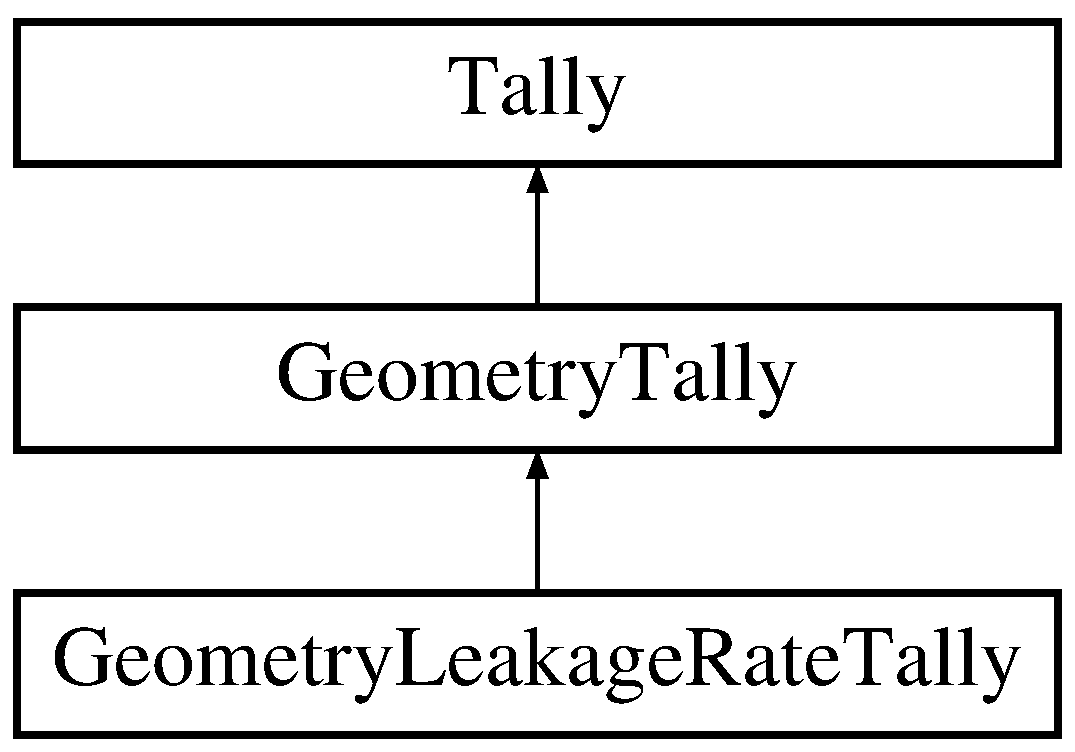
\includegraphics[height=3.000000cm]{classGeometryLeakageRateTally}
\end{center}
\end{figure}
\subsection*{Public Member Functions}
\begin{DoxyCompactItemize}
\item 
\hyperlink{classGeometryLeakageRateTally_a3fd9dfc7a6b11686d6941d922fbfdb56}{Geometry\-Leakage\-Rate\-Tally} (\hyperlink{classGeometry}{Geometry} $\ast$geometry, const char $\ast$tally\-\_\-name=(char $\ast$)\char`\"{}\char`\"{})
\begin{DoxyCompactList}\small\item\em \hyperlink{classGeometryLeakageRateTally}{Geometry\-Leakage\-Rate\-Tally} constructor calls the \hyperlink{classGeometryTally}{Geometry\-Tally} constructor and \hyperlink{classTally}{Tally} constructors and sets the tally type to L\-E\-A\-K\-A\-G\-E\-\_\-\-R\-A\-T\-E. \end{DoxyCompactList}\item 
void \hyperlink{classGeometryLeakageRateTally_a19498479ed8c16606515fa47bf45a726}{tally} (\hyperlink{structneutron}{neutron} $\ast$\hyperlink{structneutron}{neutron})
\begin{DoxyCompactList}\small\item\em \hyperlink{classTally}{Tally} the geometry leakage rate by incrementing the tally by $ DB^2 $ at the neutron's energy. \end{DoxyCompactList}\end{DoxyCompactItemize}
\subsection*{Additional Inherited Members}


\subsection{Detailed Description}
A class for tallying the leakage rate for the geometry. 

\subsection{Constructor \& Destructor Documentation}
\hypertarget{classGeometryLeakageRateTally_a3fd9dfc7a6b11686d6941d922fbfdb56}{\index{Geometry\-Leakage\-Rate\-Tally@{Geometry\-Leakage\-Rate\-Tally}!Geometry\-Leakage\-Rate\-Tally@{Geometry\-Leakage\-Rate\-Tally}}
\index{Geometry\-Leakage\-Rate\-Tally@{Geometry\-Leakage\-Rate\-Tally}!GeometryLeakageRateTally@{Geometry\-Leakage\-Rate\-Tally}}
\subsubsection[{Geometry\-Leakage\-Rate\-Tally}]{\setlength{\rightskip}{0pt plus 5cm}Geometry\-Leakage\-Rate\-Tally\-::\-Geometry\-Leakage\-Rate\-Tally (
\begin{DoxyParamCaption}
\item[{{\bf Geometry} $\ast$}]{geometry, }
\item[{const char $\ast$}]{tally\-\_\-name = {\ttfamily (char$\ast$)\char`\"{}\char`\"{}}}
\end{DoxyParamCaption}
)\hspace{0.3cm}{\ttfamily [inline]}}}\label{classGeometryLeakageRateTally_a3fd9dfc7a6b11686d6941d922fbfdb56}


\hyperlink{classGeometryLeakageRateTally}{Geometry\-Leakage\-Rate\-Tally} constructor calls the \hyperlink{classGeometryTally}{Geometry\-Tally} constructor and \hyperlink{classTally}{Tally} constructors and sets the tally type to L\-E\-A\-K\-A\-G\-E\-\_\-\-R\-A\-T\-E. 


\begin{DoxyParams}{Parameters}
{\em geometry} & a pointer to the geometry within which to tally \\
\hline
{\em tally\-\_\-name} & a character array for the tally name (optional) \\
\hline
\end{DoxyParams}


\subsection{Member Function Documentation}
\hypertarget{classGeometryLeakageRateTally_a19498479ed8c16606515fa47bf45a726}{\index{Geometry\-Leakage\-Rate\-Tally@{Geometry\-Leakage\-Rate\-Tally}!tally@{tally}}
\index{tally@{tally}!GeometryLeakageRateTally@{Geometry\-Leakage\-Rate\-Tally}}
\subsubsection[{tally}]{\setlength{\rightskip}{0pt plus 5cm}void Geometry\-Leakage\-Rate\-Tally\-::tally (
\begin{DoxyParamCaption}
\item[{{\bf neutron} $\ast$}]{neutron}
\end{DoxyParamCaption}
)\hspace{0.3cm}{\ttfamily [virtual]}}}\label{classGeometryLeakageRateTally_a19498479ed8c16606515fa47bf45a726}


\hyperlink{classTally}{Tally} the geometry leakage rate by incrementing the tally by $ DB^2 $ at the neutron's energy. 


\begin{DoxyParams}{Parameters}
{\em neutron} & the neutron of interest \\
\hline
\end{DoxyParams}


Implements \hyperlink{classGeometryTally_a3f79423e0c1e1eb87109c6937bdfa5c8}{Geometry\-Tally}.



The documentation for this class was generated from the following files\-:\begin{DoxyCompactItemize}
\item 
\hyperlink{Tally_8h}{Tally.\-h}\item 
Tally.\-cpp\end{DoxyCompactItemize}

\hypertarget{classGeometryTally}{\section{Geometry\-Tally Class Reference}
\label{classGeometryTally}\index{Geometry\-Tally@{Geometry\-Tally}}
}


An abstract class for tallies with M\-A\-T\-E\-R\-I\-A\-L domain type.  




{\ttfamily \#include \char`\"{}pinspec/src/\-Tally.\-h\char`\"{}}

Inheritance diagram for Geometry\-Tally\-:\begin{figure}[H]
\begin{center}
\leavevmode
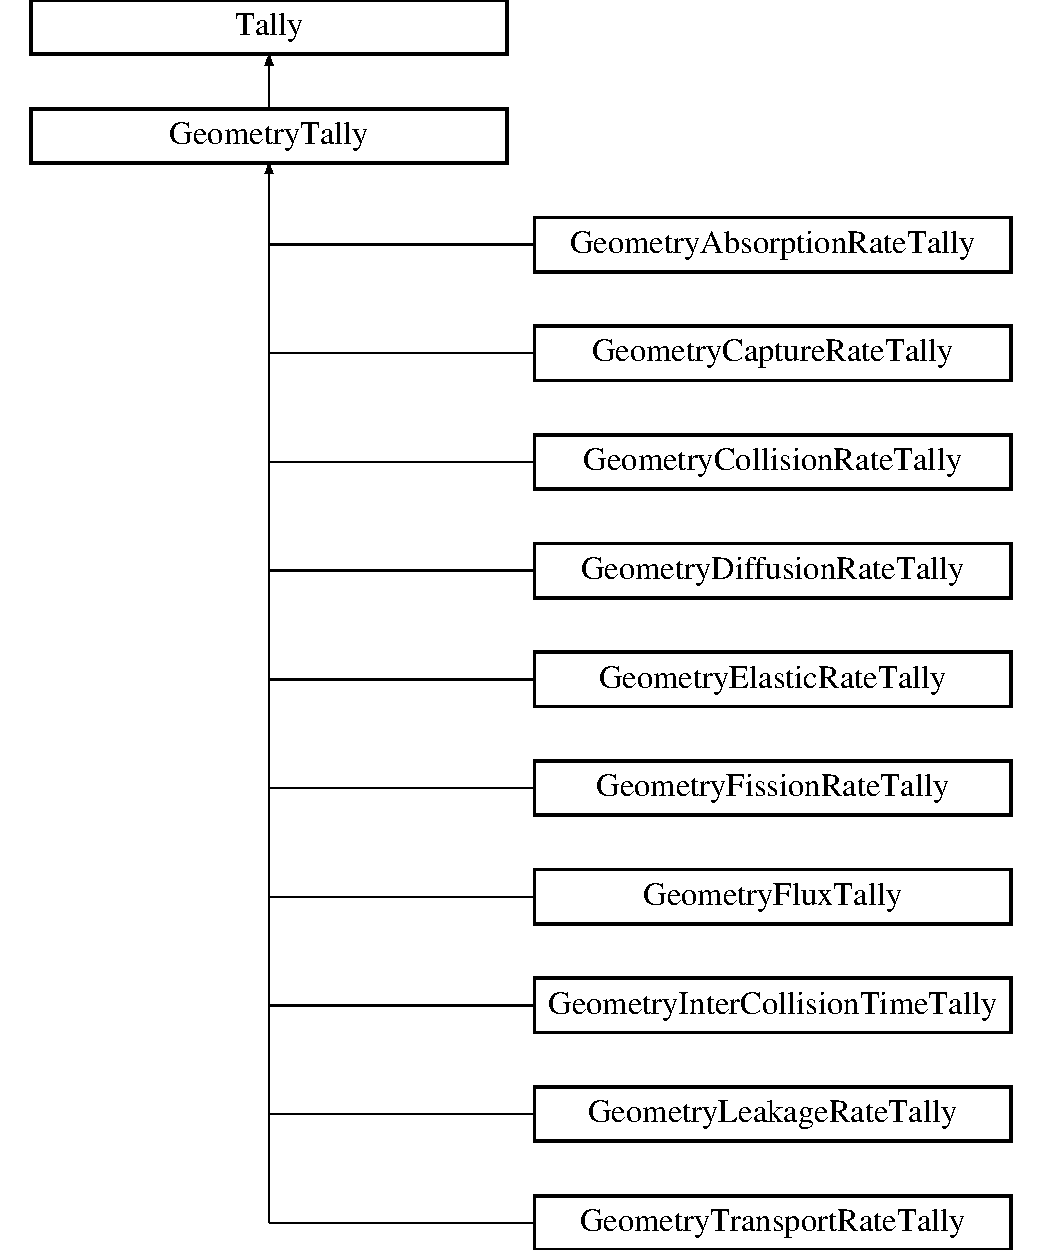
\includegraphics[height=12.000000cm]{classGeometryTally}
\end{center}
\end{figure}
\subsection*{Public Member Functions}
\begin{DoxyCompactItemize}
\item 
\hyperlink{classGeometryTally_a442edb7b6ab999650005393b5d5a3a20}{Geometry\-Tally} (\hyperlink{classGeometry}{Geometry} $\ast$geometry, const char $\ast$tally\-\_\-name=(char $\ast$)\char`\"{}\char`\"{})
\begin{DoxyCompactList}\small\item\em \hyperlink{classGeometryTally}{Geometry\-Tally} constructor calls the \hyperlink{classTally}{Tally} constructor and sets the tally domain to G\-E\-O\-M\-E\-T\-R\-Y. \end{DoxyCompactList}\item 
\hyperlink{classGeometry}{Geometry} $\ast$ \hyperlink{classGeometryTally_a4fd85a51d65e5b3edfe8931351e01d93}{get\-Geometry} ()
\begin{DoxyCompactList}\small\item\em Returns the geometry in which this tally resides. \end{DoxyCompactList}\item 
\hypertarget{classGeometryTally_a3f79423e0c1e1eb87109c6937bdfa5c8}{virtual void \hyperlink{classGeometryTally_a3f79423e0c1e1eb87109c6937bdfa5c8}{tally} (\hyperlink{structneutron}{neutron} $\ast$\hyperlink{structneutron}{neutron})=0}\label{classGeometryTally_a3f79423e0c1e1eb87109c6937bdfa5c8}

\begin{DoxyCompactList}\small\item\em A method to tally a neutron to be implemented by subclasses. \end{DoxyCompactList}\end{DoxyCompactItemize}
\subsection*{Protected Attributes}
\begin{DoxyCompactItemize}
\item 
\hyperlink{classGeometry}{Geometry} $\ast$ \hyperlink{classGeometryTally_ab2ed248e810a207e6037017a01b757f5}{\-\_\-geometry}
\end{DoxyCompactItemize}


\subsection{Detailed Description}
An abstract class for tallies with M\-A\-T\-E\-R\-I\-A\-L domain type. 

A \hyperlink{classGeometryTally}{Geometry\-Tally} is for tallying within a geometry. The \hyperlink{classGeometryTally}{Geometry\-Tally} is an abstract class and must be implemented for each tally\-Type. 

\subsection{Constructor \& Destructor Documentation}
\hypertarget{classGeometryTally_a442edb7b6ab999650005393b5d5a3a20}{\index{Geometry\-Tally@{Geometry\-Tally}!Geometry\-Tally@{Geometry\-Tally}}
\index{Geometry\-Tally@{Geometry\-Tally}!GeometryTally@{Geometry\-Tally}}
\subsubsection[{Geometry\-Tally}]{\setlength{\rightskip}{0pt plus 5cm}Geometry\-Tally\-::\-Geometry\-Tally (
\begin{DoxyParamCaption}
\item[{{\bf Geometry} $\ast$}]{geometry, }
\item[{const char $\ast$}]{tally\-\_\-name = {\ttfamily (char$\ast$)\char`\"{}\char`\"{}}}
\end{DoxyParamCaption}
)\hspace{0.3cm}{\ttfamily [inline]}}}\label{classGeometryTally_a442edb7b6ab999650005393b5d5a3a20}


\hyperlink{classGeometryTally}{Geometry\-Tally} constructor calls the \hyperlink{classTally}{Tally} constructor and sets the tally domain to G\-E\-O\-M\-E\-T\-R\-Y. 


\begin{DoxyParams}{Parameters}
{\em geometry} & a pointer to the geometry within which to tally \\
\hline
{\em tally\-\_\-name} & a character array for the tally name (optional) \\
\hline
\end{DoxyParams}


\subsection{Member Function Documentation}
\hypertarget{classGeometryTally_a4fd85a51d65e5b3edfe8931351e01d93}{\index{Geometry\-Tally@{Geometry\-Tally}!get\-Geometry@{get\-Geometry}}
\index{get\-Geometry@{get\-Geometry}!GeometryTally@{Geometry\-Tally}}
\subsubsection[{get\-Geometry}]{\setlength{\rightskip}{0pt plus 5cm}{\bf Geometry}$\ast$ Geometry\-Tally\-::get\-Geometry (
\begin{DoxyParamCaption}
{}
\end{DoxyParamCaption}
)\hspace{0.3cm}{\ttfamily [inline]}}}\label{classGeometryTally_a4fd85a51d65e5b3edfe8931351e01d93}


Returns the geometry in which this tally resides. 

\begin{DoxyReturn}{Returns}
a pointer to the geometry 
\end{DoxyReturn}


\subsection{Member Data Documentation}
\hypertarget{classGeometryTally_ab2ed248e810a207e6037017a01b757f5}{\index{Geometry\-Tally@{Geometry\-Tally}!\-\_\-geometry@{\-\_\-geometry}}
\index{\-\_\-geometry@{\-\_\-geometry}!GeometryTally@{Geometry\-Tally}}
\subsubsection[{\-\_\-geometry}]{\setlength{\rightskip}{0pt plus 5cm}{\bf Geometry}$\ast$ Geometry\-Tally\-::\-\_\-geometry\hspace{0.3cm}{\ttfamily [protected]}}}\label{classGeometryTally_ab2ed248e810a207e6037017a01b757f5}
A pointer to the geometry in which this tally resides 

The documentation for this class was generated from the following file\-:\begin{DoxyCompactItemize}
\item 
pinspec/src/\hyperlink{Tally_8h}{Tally.\-h}\end{DoxyCompactItemize}

\hypertarget{classGeometryTransportRateTally}{\section{Geometry\-Transport\-Rate\-Tally Class Reference}
\label{classGeometryTransportRateTally}\index{Geometry\-Transport\-Rate\-Tally@{Geometry\-Transport\-Rate\-Tally}}
}


A class for tallying the transport rate within the geometry.  




{\ttfamily \#include \char`\"{}pinspec/src/\-Tally.\-h\char`\"{}}

Inheritance diagram for Geometry\-Transport\-Rate\-Tally\-:\begin{figure}[H]
\begin{center}
\leavevmode
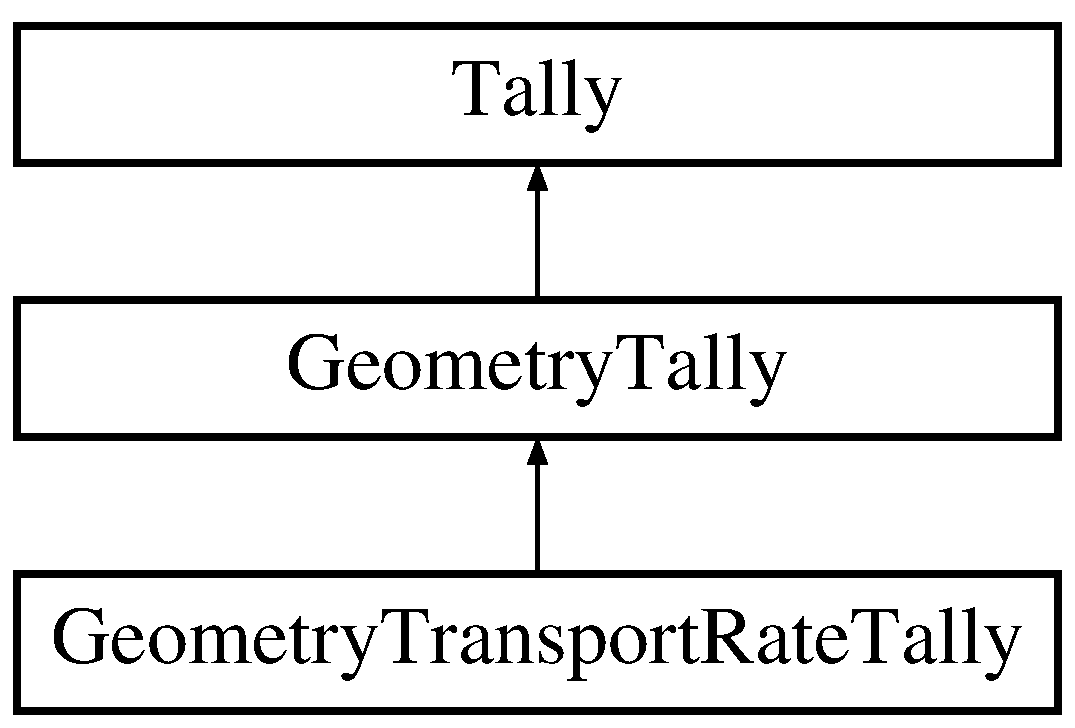
\includegraphics[height=3.000000cm]{classGeometryTransportRateTally}
\end{center}
\end{figure}
\subsection*{Public Member Functions}
\begin{DoxyCompactItemize}
\item 
\hyperlink{classGeometryTransportRateTally_a04cb0a51c0a30bfb90966ea9f35c687c}{Geometry\-Transport\-Rate\-Tally} (\hyperlink{classGeometry}{Geometry} $\ast$geometry, const char $\ast$tally\-\_\-name=(char $\ast$)\char`\"{}\char`\"{})
\begin{DoxyCompactList}\small\item\em \hyperlink{classGeometryTransportRateTally}{Geometry\-Transport\-Rate\-Tally} constructor calls the \hyperlink{classGeometryTally}{Geometry\-Tally} constructor and \hyperlink{classTally}{Tally} constructors and sets the tally type to T\-R\-A\-N\-S\-P\-O\-R\-T\-\_\-\-R\-A\-T\-E. \end{DoxyCompactList}\item 
void \hyperlink{classGeometryTransportRateTally_ab634a607b837e7e4a8637af0d7ab5d74}{tally} (\hyperlink{structneutron}{neutron} $\ast$\hyperlink{structneutron}{neutron})
\begin{DoxyCompactList}\small\item\em \hyperlink{classTally}{Tally} the geometry transport rate by incrementing the tally by $ \frac{\Sigma_tr}{\Sigma_t} $ at the neutron's energy. \end{DoxyCompactList}\end{DoxyCompactItemize}
\subsection*{Additional Inherited Members}


\subsection{Detailed Description}
A class for tallying the transport rate within the geometry. 

\subsection{Constructor \& Destructor Documentation}
\hypertarget{classGeometryTransportRateTally_a04cb0a51c0a30bfb90966ea9f35c687c}{\index{Geometry\-Transport\-Rate\-Tally@{Geometry\-Transport\-Rate\-Tally}!Geometry\-Transport\-Rate\-Tally@{Geometry\-Transport\-Rate\-Tally}}
\index{Geometry\-Transport\-Rate\-Tally@{Geometry\-Transport\-Rate\-Tally}!GeometryTransportRateTally@{Geometry\-Transport\-Rate\-Tally}}
\subsubsection[{Geometry\-Transport\-Rate\-Tally}]{\setlength{\rightskip}{0pt plus 5cm}Geometry\-Transport\-Rate\-Tally\-::\-Geometry\-Transport\-Rate\-Tally (
\begin{DoxyParamCaption}
\item[{{\bf Geometry} $\ast$}]{geometry, }
\item[{const char $\ast$}]{tally\-\_\-name = {\ttfamily (char$\ast$)\char`\"{}\char`\"{}}}
\end{DoxyParamCaption}
)\hspace{0.3cm}{\ttfamily [inline]}}}\label{classGeometryTransportRateTally_a04cb0a51c0a30bfb90966ea9f35c687c}


\hyperlink{classGeometryTransportRateTally}{Geometry\-Transport\-Rate\-Tally} constructor calls the \hyperlink{classGeometryTally}{Geometry\-Tally} constructor and \hyperlink{classTally}{Tally} constructors and sets the tally type to T\-R\-A\-N\-S\-P\-O\-R\-T\-\_\-\-R\-A\-T\-E. 


\begin{DoxyParams}{Parameters}
{\em geometry} & a pointer to the geometry within which to tally \\
\hline
{\em tally\-\_\-name} & a character array for the tally name (optional) \\
\hline
\end{DoxyParams}


\subsection{Member Function Documentation}
\hypertarget{classGeometryTransportRateTally_ab634a607b837e7e4a8637af0d7ab5d74}{\index{Geometry\-Transport\-Rate\-Tally@{Geometry\-Transport\-Rate\-Tally}!tally@{tally}}
\index{tally@{tally}!GeometryTransportRateTally@{Geometry\-Transport\-Rate\-Tally}}
\subsubsection[{tally}]{\setlength{\rightskip}{0pt plus 5cm}void Geometry\-Transport\-Rate\-Tally\-::tally (
\begin{DoxyParamCaption}
\item[{{\bf neutron} $\ast$}]{neutron}
\end{DoxyParamCaption}
)\hspace{0.3cm}{\ttfamily [virtual]}}}\label{classGeometryTransportRateTally_ab634a607b837e7e4a8637af0d7ab5d74}


\hyperlink{classTally}{Tally} the geometry transport rate by incrementing the tally by $ \frac{\Sigma_tr}{\Sigma_t} $ at the neutron's energy. 


\begin{DoxyParams}{Parameters}
{\em neutron} & the neutron of interest \\
\hline
\end{DoxyParams}


Implements \hyperlink{classGeometryTally_a3f79423e0c1e1eb87109c6937bdfa5c8}{Geometry\-Tally}.



The documentation for this class was generated from the following files\-:\begin{DoxyCompactItemize}
\item 
pinspec/src/\hyperlink{Tally_8h}{Tally.\-h}\item 
pinspec/src/Tally.\-cpp\end{DoxyCompactItemize}

\hypertarget{classpinspec_1_1process_1_1GroupXS}{\section{pinspec.\-process.\-Group\-X\-S Class Reference}
\label{classpinspec_1_1process_1_1GroupXS}\index{pinspec.\-process.\-Group\-X\-S@{pinspec.\-process.\-Group\-X\-S}}
}


A multi-\/group cross-\/section for a certain reaction rate.  




{\ttfamily \#include \char`\"{}pinspec/process.\-py\char`\"{}}

\subsection*{Public Member Functions}
\begin{DoxyCompactItemize}
\item 
def \hyperlink{classpinspec_1_1process_1_1GroupXS_ad81cb8d5201650c809f300a4af11921f}{\-\_\-\-\_\-init\-\_\-\-\_\-}
\begin{DoxyCompactList}\small\item\em The group cross-\/section constructor. \end{DoxyCompactList}\item 
def \hyperlink{classpinspec_1_1process_1_1GroupXS_a86e9d4738e35a82b241a3c7b79882466}{compute\-Group\-X\-S}
\begin{DoxyCompactList}\small\item\em Computes the multigroup cross-\/sections from the two tallies. \end{DoxyCompactList}\item 
def \hyperlink{classpinspec_1_1process_1_1GroupXS_ae52730b41f0003d4295486cba6ec7438}{set\-Name}
\begin{DoxyCompactList}\small\item\em Sets the name of this group cross-\/section. \end{DoxyCompactList}\item 
def \hyperlink{classpinspec_1_1process_1_1GroupXS_ad184b77037578e558a6698a8311bc284}{get\-Name}
\begin{DoxyCompactList}\small\item\em Returns the name of the \hyperlink{classpinspec_1_1process_1_1GroupXS}{Group\-X\-S} object. \end{DoxyCompactList}\item 
def \hyperlink{classpinspec_1_1process_1_1GroupXS_ae4ae5eda18c6bbc4151d95525ce37394}{get\-Num\-X\-S}
\begin{DoxyCompactList}\small\item\em Returns the number of multi-\/group cross-\/section values. \end{DoxyCompactList}\item 
def \hyperlink{classpinspec_1_1process_1_1GroupXS_a2722f0f4c1e6e7ffdcd3485052ba59b7}{get\-X\-S}
\begin{DoxyCompactList}\small\item\em Retrurns an array of the batch-\/averaged multi-\/group cross-\/sections. \end{DoxyCompactList}\item 
def \hyperlink{classpinspec_1_1process_1_1GroupXS_ac26ac7b80a4498b75fc535f112bf1ff4}{get\-Variances}
\begin{DoxyCompactList}\small\item\em Returns an array of the multi-\/group cross-\/section variances. \end{DoxyCompactList}\item 
def \hyperlink{classpinspec_1_1process_1_1GroupXS_af74a0da1fab21995e6105762aa21eed9}{get\-Standard\-Deviation}
\begin{DoxyCompactList}\small\item\em Returns an array of the multi-\/group cross-\/section standard deviations. \end{DoxyCompactList}\item 
def \hyperlink{classpinspec_1_1process_1_1GroupXS_a0adae8d5005d0534ccb3dcb3302bef6c}{get\-Relative\-Error}
\begin{DoxyCompactList}\small\item\em Returns an array of the multi-\/group cross-\/section relative errors. \end{DoxyCompactList}\item 
def \hyperlink{classpinspec_1_1process_1_1GroupXS_a9a56a3b63e126b65ce191ca7dbdcda32}{get\-Energy\-Bands}
\begin{DoxyCompactList}\small\item\em Returns an array of the multi-\/group cross-\/section energy band centers. \end{DoxyCompactList}\item 
def \hyperlink{classpinspec_1_1process_1_1GroupXS_aee3cc4641d6f9709c25cfa4e6fbbba08}{get\-Group\-X\-S}
\begin{DoxyCompactList}\small\item\em Returns a reference to this \hyperlink{classpinspec_1_1process_1_1GroupXS}{Group\-X\-S} object. \end{DoxyCompactList}\item 
def \hyperlink{classpinspec_1_1process_1_1GroupXS_a2918792badce34f95584a70d89aa71f7}{print\-X\-S}
\begin{DoxyCompactList}\small\item\em Prints a formatted table of the multi-\/group cross-\/sections to the screen. \end{DoxyCompactList}\item 
def \hyperlink{classpinspec_1_1process_1_1GroupXS_a6b64121b4d0efaf6b3e86587ecde0273}{output\-X\-Sto\-File}
\begin{DoxyCompactList}\small\item\em Prints the multi-\/group cross-\/section data and batch statistics to a file. \end{DoxyCompactList}\end{DoxyCompactItemize}
\subsection*{Private Attributes}
\begin{DoxyCompactItemize}
\item 
\hypertarget{classpinspec_1_1process_1_1GroupXS_ae1ec6f536e2a123c5e050313681364ce}{\hyperlink{classpinspec_1_1process_1_1GroupXS_ae1ec6f536e2a123c5e050313681364ce}{\-\_\-name}}\label{classpinspec_1_1process_1_1GroupXS_ae1ec6f536e2a123c5e050313681364ce}

\begin{DoxyCompactList}\small\item\em The name of the multi-\/group cross-\/section. \end{DoxyCompactList}\item 
\hypertarget{classpinspec_1_1process_1_1GroupXS_ad6f901eaff624ea2d59280d198bbca09}{\hyperlink{classpinspec_1_1process_1_1GroupXS_ad6f901eaff624ea2d59280d198bbca09}{\-\_\-xs}}\label{classpinspec_1_1process_1_1GroupXS_ad6f901eaff624ea2d59280d198bbca09}

\begin{DoxyCompactList}\small\item\em The D\-E\-R\-I\-V\-E\-D tally used to store the multi-\/group cross-\/sections. \end{DoxyCompactList}\item 
\hypertarget{classpinspec_1_1process_1_1GroupXS_acc9c47ded2fb3c3e8d27b8ca1652962a}{\hyperlink{classpinspec_1_1process_1_1GroupXS_acc9c47ded2fb3c3e8d27b8ca1652962a}{\-\_\-flux}}\label{classpinspec_1_1process_1_1GroupXS_acc9c47ded2fb3c3e8d27b8ca1652962a}

\begin{DoxyCompactList}\small\item\em The F\-L\-U\-X tally used to compute the multi-\/group cross-\/sections. \end{DoxyCompactList}\item 
\hypertarget{classpinspec_1_1process_1_1GroupXS_a72b491dd81618cc213b4f397d3a73b14}{\hyperlink{classpinspec_1_1process_1_1GroupXS_a72b491dd81618cc213b4f397d3a73b14}{\-\_\-rate}}\label{classpinspec_1_1process_1_1GroupXS_a72b491dd81618cc213b4f397d3a73b14}

\begin{DoxyCompactList}\small\item\em The R\-E\-A\-C\-T\-I\-O\-N\-\_\-\-R\-A\-T\-E tally used to compute the multi-\/group cross-\/sections. \end{DoxyCompactList}\item 
\hypertarget{classpinspec_1_1process_1_1GroupXS_aec56586bd4e0a90d9d5ce97ad6c40595}{\hyperlink{classpinspec_1_1process_1_1GroupXS_aec56586bd4e0a90d9d5ce97ad6c40595}{\-\_\-num\-\_\-xs}}\label{classpinspec_1_1process_1_1GroupXS_aec56586bd4e0a90d9d5ce97ad6c40595}

\begin{DoxyCompactList}\small\item\em The number of multi-\/group cross-\/sections. \end{DoxyCompactList}\end{DoxyCompactItemize}


\subsection{Detailed Description}
A multi-\/group cross-\/section for a certain reaction rate. 

This class represents a multi-\/group cross-\/section with some energy bands for a certain reaction rate. By default, the group cross-\/section is a macroscopic cross-\/section $ (cm^{-1}) $. 

\subsection{Constructor \& Destructor Documentation}
\hypertarget{classpinspec_1_1process_1_1GroupXS_ad81cb8d5201650c809f300a4af11921f}{\index{pinspec\-::process\-::\-Group\-X\-S@{pinspec\-::process\-::\-Group\-X\-S}!\-\_\-\-\_\-init\-\_\-\-\_\-@{\-\_\-\-\_\-init\-\_\-\-\_\-}}
\index{\-\_\-\-\_\-init\-\_\-\-\_\-@{\-\_\-\-\_\-init\-\_\-\-\_\-}!pinspec::process::GroupXS@{pinspec\-::process\-::\-Group\-X\-S}}
\subsubsection[{\-\_\-\-\_\-init\-\_\-\-\_\-}]{\setlength{\rightskip}{0pt plus 5cm}def pinspec.\-process.\-Group\-X\-S.\-\_\-\-\_\-init\-\_\-\-\_\- (
\begin{DoxyParamCaption}
\item[{}]{self, }
\item[{}]{tally1, }
\item[{}]{tally2, }
\item[{}]{name = {\ttfamily ''}}
\end{DoxyParamCaption}
)}}\label{classpinspec_1_1process_1_1GroupXS_ad81cb8d5201650c809f300a4af11921f}


The group cross-\/section constructor. 


\begin{DoxyParams}{Parameters}
{\em self} & the \hyperlink{classpinspec_1_1process_1_1GroupXS}{Group\-X\-S} object pointer \\
\hline
{\em tally1} & one of the tallies needed to compute a multi-\/group cross-\/section \\
\hline
{\em tally2} & one of the tallies needed to compute a multi-\/group cross-\/section \\
\hline
{\em name} & an optional argument string for the name of the multi-\/group cross-\/section \\
\hline
\end{DoxyParams}


\subsection{Member Function Documentation}
\hypertarget{classpinspec_1_1process_1_1GroupXS_a86e9d4738e35a82b241a3c7b79882466}{\index{pinspec\-::process\-::\-Group\-X\-S@{pinspec\-::process\-::\-Group\-X\-S}!compute\-Group\-X\-S@{compute\-Group\-X\-S}}
\index{compute\-Group\-X\-S@{compute\-Group\-X\-S}!pinspec::process::GroupXS@{pinspec\-::process\-::\-Group\-X\-S}}
\subsubsection[{compute\-Group\-X\-S}]{\setlength{\rightskip}{0pt plus 5cm}def pinspec.\-process.\-Group\-X\-S.\-compute\-Group\-X\-S (
\begin{DoxyParamCaption}
\item[{}]{self, }
\item[{}]{tally1, }
\item[{}]{tally2}
\end{DoxyParamCaption}
)}}\label{classpinspec_1_1process_1_1GroupXS_a86e9d4738e35a82b241a3c7b79882466}


Computes the multigroup cross-\/sections from the two tallies. 

This method checks that one of the tallies input is a reaction rate and the other is a flux, with the same bin edges. If the batch statistics for both tallies have been computed, it computes the multigroup cross-\/section as follows\-:


\begin{DoxyCode}
sigma\_groups = reaction\_rate / flux
\end{DoxyCode}



\begin{DoxyParams}{Parameters}
{\em self} & the \hyperlink{classpinspec_1_1process_1_1GroupXS}{Group\-X\-S} object pointer \\
\hline
{\em tally1} & one of the tallies needed to compute a multi-\/group cross-\/section \\
\hline
{\em tally2} & one of the tallies needed to compute a multi-\/group cross-\/section \\
\hline
\end{DoxyParams}
\hypertarget{classpinspec_1_1process_1_1GroupXS_a9a56a3b63e126b65ce191ca7dbdcda32}{\index{pinspec\-::process\-::\-Group\-X\-S@{pinspec\-::process\-::\-Group\-X\-S}!get\-Energy\-Bands@{get\-Energy\-Bands}}
\index{get\-Energy\-Bands@{get\-Energy\-Bands}!pinspec::process::GroupXS@{pinspec\-::process\-::\-Group\-X\-S}}
\subsubsection[{get\-Energy\-Bands}]{\setlength{\rightskip}{0pt plus 5cm}def pinspec.\-process.\-Group\-X\-S.\-get\-Energy\-Bands (
\begin{DoxyParamCaption}
\item[{}]{self}
\end{DoxyParamCaption}
)}}\label{classpinspec_1_1process_1_1GroupXS_a9a56a3b63e126b65ce191ca7dbdcda32}


Returns an array of the multi-\/group cross-\/section energy band centers. 


\begin{DoxyParams}{Parameters}
{\em self} & the \hyperlink{classpinspec_1_1process_1_1GroupXS}{Group\-X\-S} object pointer \\
\hline
\end{DoxyParams}
\begin{DoxyReturn}{Returns}
a numpy array of the multi-\/group cross-\/section energy band centers def get\-Energy\-Bands\-Centers(self)\-: Returns an array of the multi-\/group cross-\/section energy band values. 
\end{DoxyReturn}

\begin{DoxyParams}{Parameters}
{\em self} & the \hyperlink{classpinspec_1_1process_1_1GroupXS}{Group\-X\-S} object pointer \\
\hline
\end{DoxyParams}
\begin{DoxyReturn}{Returns}
a numpy array of the multi-\/group cross-\/section energy band values 
\end{DoxyReturn}
\hypertarget{classpinspec_1_1process_1_1GroupXS_aee3cc4641d6f9709c25cfa4e6fbbba08}{\index{pinspec\-::process\-::\-Group\-X\-S@{pinspec\-::process\-::\-Group\-X\-S}!get\-Group\-X\-S@{get\-Group\-X\-S}}
\index{get\-Group\-X\-S@{get\-Group\-X\-S}!pinspec::process::GroupXS@{pinspec\-::process\-::\-Group\-X\-S}}
\subsubsection[{get\-Group\-X\-S}]{\setlength{\rightskip}{0pt plus 5cm}def pinspec.\-process.\-Group\-X\-S.\-get\-Group\-X\-S (
\begin{DoxyParamCaption}
\item[{}]{self}
\end{DoxyParamCaption}
)}}\label{classpinspec_1_1process_1_1GroupXS_aee3cc4641d6f9709c25cfa4e6fbbba08}


Returns a reference to this \hyperlink{classpinspec_1_1process_1_1GroupXS}{Group\-X\-S} object. 


\begin{DoxyParams}{Parameters}
{\em self} & \hyperlink{classpinspec_1_1process_1_1GroupXS}{Group\-X\-S} the object pointer \\
\hline
\end{DoxyParams}
\begin{DoxyReturn}{Returns}
a reference to the \hyperlink{classpinspec_1_1process_1_1GroupXS}{Group\-X\-S} object 
\end{DoxyReturn}
\hypertarget{classpinspec_1_1process_1_1GroupXS_ad184b77037578e558a6698a8311bc284}{\index{pinspec\-::process\-::\-Group\-X\-S@{pinspec\-::process\-::\-Group\-X\-S}!get\-Name@{get\-Name}}
\index{get\-Name@{get\-Name}!pinspec::process::GroupXS@{pinspec\-::process\-::\-Group\-X\-S}}
\subsubsection[{get\-Name}]{\setlength{\rightskip}{0pt plus 5cm}def pinspec.\-process.\-Group\-X\-S.\-get\-Name (
\begin{DoxyParamCaption}
\item[{}]{self}
\end{DoxyParamCaption}
)}}\label{classpinspec_1_1process_1_1GroupXS_ad184b77037578e558a6698a8311bc284}


Returns the name of the \hyperlink{classpinspec_1_1process_1_1GroupXS}{Group\-X\-S} object. 

Returns an empty string if no name has been specified by the user. 
\begin{DoxyParams}{Parameters}
{\em self} & the \hyperlink{classpinspec_1_1process_1_1GroupXS}{Group\-X\-S} object pointer \\
\hline
\end{DoxyParams}
\begin{DoxyReturn}{Returns}
a string with the name of the \hyperlink{classpinspec_1_1process_1_1GroupXS}{Group\-X\-S} 
\end{DoxyReturn}
\hypertarget{classpinspec_1_1process_1_1GroupXS_ae4ae5eda18c6bbc4151d95525ce37394}{\index{pinspec\-::process\-::\-Group\-X\-S@{pinspec\-::process\-::\-Group\-X\-S}!get\-Num\-X\-S@{get\-Num\-X\-S}}
\index{get\-Num\-X\-S@{get\-Num\-X\-S}!pinspec::process::GroupXS@{pinspec\-::process\-::\-Group\-X\-S}}
\subsubsection[{get\-Num\-X\-S}]{\setlength{\rightskip}{0pt plus 5cm}def pinspec.\-process.\-Group\-X\-S.\-get\-Num\-X\-S (
\begin{DoxyParamCaption}
\item[{}]{self}
\end{DoxyParamCaption}
)}}\label{classpinspec_1_1process_1_1GroupXS_ae4ae5eda18c6bbc4151d95525ce37394}


Returns the number of multi-\/group cross-\/section values. 


\begin{DoxyParams}{Parameters}
{\em self} & the \hyperlink{classpinspec_1_1process_1_1GroupXS}{Group\-X\-S} object pointer \\
\hline
\end{DoxyParams}
\begin{DoxyReturn}{Returns}
the number of multi-\/group cross-\/section values 
\end{DoxyReturn}
\hypertarget{classpinspec_1_1process_1_1GroupXS_a0adae8d5005d0534ccb3dcb3302bef6c}{\index{pinspec\-::process\-::\-Group\-X\-S@{pinspec\-::process\-::\-Group\-X\-S}!get\-Relative\-Error@{get\-Relative\-Error}}
\index{get\-Relative\-Error@{get\-Relative\-Error}!pinspec::process::GroupXS@{pinspec\-::process\-::\-Group\-X\-S}}
\subsubsection[{get\-Relative\-Error}]{\setlength{\rightskip}{0pt plus 5cm}def pinspec.\-process.\-Group\-X\-S.\-get\-Relative\-Error (
\begin{DoxyParamCaption}
\item[{}]{self}
\end{DoxyParamCaption}
)}}\label{classpinspec_1_1process_1_1GroupXS_a0adae8d5005d0534ccb3dcb3302bef6c}


Returns an array of the multi-\/group cross-\/section relative errors. 


\begin{DoxyParams}{Parameters}
{\em self} & the \hyperlink{classpinspec_1_1process_1_1GroupXS}{Group\-X\-S} object pointer \\
\hline
\end{DoxyParams}
\begin{DoxyReturn}{Returns}
a numpy array of the multi-\/group cross-\/section relative errors 
\end{DoxyReturn}
\hypertarget{classpinspec_1_1process_1_1GroupXS_af74a0da1fab21995e6105762aa21eed9}{\index{pinspec\-::process\-::\-Group\-X\-S@{pinspec\-::process\-::\-Group\-X\-S}!get\-Standard\-Deviation@{get\-Standard\-Deviation}}
\index{get\-Standard\-Deviation@{get\-Standard\-Deviation}!pinspec::process::GroupXS@{pinspec\-::process\-::\-Group\-X\-S}}
\subsubsection[{get\-Standard\-Deviation}]{\setlength{\rightskip}{0pt plus 5cm}def pinspec.\-process.\-Group\-X\-S.\-get\-Standard\-Deviation (
\begin{DoxyParamCaption}
\item[{}]{self}
\end{DoxyParamCaption}
)}}\label{classpinspec_1_1process_1_1GroupXS_af74a0da1fab21995e6105762aa21eed9}


Returns an array of the multi-\/group cross-\/section standard deviations. 


\begin{DoxyParams}{Parameters}
{\em self} & the \hyperlink{classpinspec_1_1process_1_1GroupXS}{Group\-X\-S} object pointer \\
\hline
\end{DoxyParams}
\begin{DoxyReturn}{Returns}
a numpy array of the multi-\/group cross-\/section standard deviations 
\end{DoxyReturn}
\hypertarget{classpinspec_1_1process_1_1GroupXS_ac26ac7b80a4498b75fc535f112bf1ff4}{\index{pinspec\-::process\-::\-Group\-X\-S@{pinspec\-::process\-::\-Group\-X\-S}!get\-Variances@{get\-Variances}}
\index{get\-Variances@{get\-Variances}!pinspec::process::GroupXS@{pinspec\-::process\-::\-Group\-X\-S}}
\subsubsection[{get\-Variances}]{\setlength{\rightskip}{0pt plus 5cm}def pinspec.\-process.\-Group\-X\-S.\-get\-Variances (
\begin{DoxyParamCaption}
\item[{}]{self}
\end{DoxyParamCaption}
)}}\label{classpinspec_1_1process_1_1GroupXS_ac26ac7b80a4498b75fc535f112bf1ff4}


Returns an array of the multi-\/group cross-\/section variances. 


\begin{DoxyParams}{Parameters}
{\em self} & the \hyperlink{classpinspec_1_1process_1_1GroupXS}{Group\-X\-S} object pointer \\
\hline
\end{DoxyParams}
\begin{DoxyReturn}{Returns}
a numpy array of the multi-\/group cross-\/section variances 
\end{DoxyReturn}
\hypertarget{classpinspec_1_1process_1_1GroupXS_a2722f0f4c1e6e7ffdcd3485052ba59b7}{\index{pinspec\-::process\-::\-Group\-X\-S@{pinspec\-::process\-::\-Group\-X\-S}!get\-X\-S@{get\-X\-S}}
\index{get\-X\-S@{get\-X\-S}!pinspec::process::GroupXS@{pinspec\-::process\-::\-Group\-X\-S}}
\subsubsection[{get\-X\-S}]{\setlength{\rightskip}{0pt plus 5cm}def pinspec.\-process.\-Group\-X\-S.\-get\-X\-S (
\begin{DoxyParamCaption}
\item[{}]{self}
\end{DoxyParamCaption}
)}}\label{classpinspec_1_1process_1_1GroupXS_a2722f0f4c1e6e7ffdcd3485052ba59b7}


Retrurns an array of the batch-\/averaged multi-\/group cross-\/sections. 


\begin{DoxyParams}{Parameters}
{\em self} & the \hyperlink{classpinspec_1_1process_1_1GroupXS}{Group\-X\-S} object pointer \\
\hline
\end{DoxyParams}
\begin{DoxyReturn}{Returns}
a numpy array of the multi-\/group cross-\/sections 
\end{DoxyReturn}
\hypertarget{classpinspec_1_1process_1_1GroupXS_a6b64121b4d0efaf6b3e86587ecde0273}{\index{pinspec\-::process\-::\-Group\-X\-S@{pinspec\-::process\-::\-Group\-X\-S}!output\-X\-Sto\-File@{output\-X\-Sto\-File}}
\index{output\-X\-Sto\-File@{output\-X\-Sto\-File}!pinspec::process::GroupXS@{pinspec\-::process\-::\-Group\-X\-S}}
\subsubsection[{output\-X\-Sto\-File}]{\setlength{\rightskip}{0pt plus 5cm}def pinspec.\-process.\-Group\-X\-S.\-output\-X\-Sto\-File (
\begin{DoxyParamCaption}
\item[{}]{self, }
\item[{}]{filename = {\ttfamily ''}}
\end{DoxyParamCaption}
)}}\label{classpinspec_1_1process_1_1GroupXS_a6b64121b4d0efaf6b3e86587ecde0273}


Prints the multi-\/group cross-\/section data and batch statistics to a file. 

Since the multi-\/group cross-\/sections are stored as a D\-E\-R\-I\-V\-E\-D tally type, this method prints the cross-\/section data to a file using the \hyperlink{classTally_a4fd93a5423286a5a9b7953cc8d1dcbcf}{Tally\-::output\-Batch\-Statistics()} method. An auto-\/generated filename will be created with the format 'tally-\/\#.data' where \# is an auto-\/incremented integer for each tally output data file created. 
\begin{DoxyParams}{Parameters}
{\em self} & the \hyperlink{classpinspec_1_1process_1_1GroupXS}{Group\-X\-S} object pointer \\
\hline
{\em filename} & An optional filename for the output file \\
\hline
\end{DoxyParams}
\hypertarget{classpinspec_1_1process_1_1GroupXS_a2918792badce34f95584a70d89aa71f7}{\index{pinspec\-::process\-::\-Group\-X\-S@{pinspec\-::process\-::\-Group\-X\-S}!print\-X\-S@{print\-X\-S}}
\index{print\-X\-S@{print\-X\-S}!pinspec::process::GroupXS@{pinspec\-::process\-::\-Group\-X\-S}}
\subsubsection[{print\-X\-S}]{\setlength{\rightskip}{0pt plus 5cm}def pinspec.\-process.\-Group\-X\-S.\-print\-X\-S (
\begin{DoxyParamCaption}
\item[{}]{self, }
\item[{}]{uncertainties = {\ttfamily False}}
\end{DoxyParamCaption}
)}}\label{classpinspec_1_1process_1_1GroupXS_a2918792badce34f95584a70d89aa71f7}


Prints a formatted table of the multi-\/group cross-\/sections to the screen. 

The multi-\/group cross-\/sections and their uncertainties (optional) will be printed as a formatted table to the screen. 
\begin{DoxyParams}{Parameters}
{\em self} & the \hyperlink{classpinspec_1_1process_1_1GroupXS}{Group\-X\-S} object pointer \\
\hline
{\em uncertainties} & whether or not to print tally statistics (default is false) \\
\hline
\end{DoxyParams}
\begin{DoxyReturn}{Returns}
a reference to the \hyperlink{classpinspec_1_1process_1_1GroupXS}{Group\-X\-S} object 
\end{DoxyReturn}
\hypertarget{classpinspec_1_1process_1_1GroupXS_ae52730b41f0003d4295486cba6ec7438}{\index{pinspec\-::process\-::\-Group\-X\-S@{pinspec\-::process\-::\-Group\-X\-S}!set\-Name@{set\-Name}}
\index{set\-Name@{set\-Name}!pinspec::process::GroupXS@{pinspec\-::process\-::\-Group\-X\-S}}
\subsubsection[{set\-Name}]{\setlength{\rightskip}{0pt plus 5cm}def pinspec.\-process.\-Group\-X\-S.\-set\-Name (
\begin{DoxyParamCaption}
\item[{}]{self, }
\item[{}]{name = {\ttfamily ''}}
\end{DoxyParamCaption}
)}}\label{classpinspec_1_1process_1_1GroupXS_ae52730b41f0003d4295486cba6ec7438}


Sets the name of this group cross-\/section. 

This is useful when one wishes to print the multi-\/group cross-\/section values to the screen or a file since it will be identifiable by the user-\/defined name. 
\begin{DoxyParams}{Parameters}
{\em self} & the \hyperlink{classpinspec_1_1process_1_1GroupXS}{Group\-X\-S} object pointer \\
\hline
{\em name} & the name of the \hyperlink{classpinspec_1_1process_1_1GroupXS}{Group\-X\-S} object \\
\hline
\end{DoxyParams}


The documentation for this class was generated from the following file\-:\begin{DoxyCompactItemize}
\item 
pinspec/\hyperlink{process_8py}{process.\-py}\end{DoxyCompactItemize}

\hypertarget{classIsotope}{\section{Isotope Class Reference}
\label{classIsotope}\index{Isotope@{Isotope}}
}


The \hyperlink{classIsotope}{Isotope} represents a nuclide at some temperature.  




{\ttfamily \#include \char`\"{}pinspec/src/\-Isotope.\-h\char`\"{}}

\subsection*{Public Member Functions}
\begin{DoxyCompactItemize}
\item 
\hyperlink{classIsotope_a51ff93cb15b7956c86dcc7a80aec52f7}{Isotope} (char $\ast$\-\_\-isotope\-\_\-name)
\begin{DoxyCompactList}\small\item\em \hyperlink{classIsotope}{Isotope} constructor. \end{DoxyCompactList}\item 
\hypertarget{classIsotope_a7b22935e0ade348ee513733eeda1fa23}{virtual \hyperlink{classIsotope_a7b22935e0ade348ee513733eeda1fa23}{$\sim$\-Isotope} ()}\label{classIsotope_a7b22935e0ade348ee513733eeda1fa23}

\begin{DoxyCompactList}\small\item\em \hyperlink{classIsotope}{Isotope} destructor deletes arrays of cross-\/section values that have been assigned to this isotope. \end{DoxyCompactList}\item 
\hypertarget{classIsotope_a8f2edf586499fff80ecee7cbdc28bd0e}{void \hyperlink{classIsotope_a8f2edf586499fff80ecee7cbdc28bd0e}{parse\-Name} ()}\label{classIsotope_a8f2edf586499fff80ecee7cbdc28bd0e}

\begin{DoxyCompactList}\small\item\em Parse input name and set atomic number for isotope. \end{DoxyCompactList}\item 
\hypertarget{classIsotope_a9adedaf6a1bd4cee536c4684d6adaf65}{void \hyperlink{classIsotope_a9adedaf6a1bd4cee536c4684d6adaf65}{make\-Fissionable} ()}\label{classIsotope_a9adedaf6a1bd4cee536c4684d6adaf65}

\begin{DoxyCompactList}\small\item\em Inform isotope that it is fissionable. \end{DoxyCompactList}\item 
char $\ast$ \hyperlink{classIsotope_a3e2ee2187d8765500876067f184e9958}{get\-Isotope\-Name} () const 
\begin{DoxyCompactList}\small\item\em Returns the name of the of isotope. \end{DoxyCompactList}\item 
int \hyperlink{classIsotope_a147b6797175aebe1971ce959e9fee09f}{get\-A} () const 
\begin{DoxyCompactList}\small\item\em Returns the atomic number of this isotope. \end{DoxyCompactList}\item 
float \hyperlink{classIsotope_ad0003d170a157b0bcbc7577803408f33}{get\-Alpha} () const 
\begin{DoxyCompactList}\small\item\em Returns the alpha $ \alpha = ((A-1)/(A+1))^2 $ values for this isotope. \end{DoxyCompactList}\item 
float \hyperlink{classIsotope_af391a8ae308eddee653ecc9015da607f}{get\-Temperature} () const 
\begin{DoxyCompactList}\small\item\em Return the temperature in degrees Kelvin for this isotope. \end{DoxyCompactList}\item 
float \hyperlink{classIsotope_a9f9a06707126591c5a8e65896bfa3552}{get\-Mu\-Average} () const 
\begin{DoxyCompactList}\small\item\em Return the average value of the cosine of the scattering angle. \end{DoxyCompactList}\item 
bool \hyperlink{classIsotope_aa8b40c46707c5989d4d834b4805e363a}{is\-Fissionable} () const 
\begin{DoxyCompactList}\small\item\em Return whether this isotope is fissionable (true) or not (false) \end{DoxyCompactList}\item 
int \hyperlink{classIsotope_aba83c46d1b7215f8cd0a3c6002e06588}{get\-Num\-X\-S\-Energies} (char $\ast$xs\-\_\-type) const 
\begin{DoxyCompactList}\small\item\em Returns the number of energies for a particular cross-\/section type. \end{DoxyCompactList}\item 
float \hyperlink{classIsotope_a53d04a9a711e4bef92c295739eeb76ab}{get\-Elastic\-X\-S} (float energy) const 
\begin{DoxyCompactList}\small\item\em Returns the microscopic elastic scattering cross-\/section value for some energy. \end{DoxyCompactList}\item 
float \hyperlink{classIsotope_a94493acad07eda936488edbffb48c976}{get\-Elastic\-X\-S} (int energy\-\_\-index) const 
\begin{DoxyCompactList}\small\item\em Returns the microscopic elastic cross-\/section value for a certain energy index in this isotope's rescaled uniform lethargy grid of cross-\/section data. \end{DoxyCompactList}\item 
float \hyperlink{classIsotope_ab0ba42960ecd18d9e6e0e995e99c2bf4}{get\-Absorption\-X\-S} (float energy) const 
\begin{DoxyCompactList}\small\item\em Returns the microscopic absorption cross-\/section value for some energy. \end{DoxyCompactList}\item 
float \hyperlink{classIsotope_a4ecbc76ad446036895ab662403214394}{get\-Absorption\-X\-S} (int energy\-\_\-index) const 
\begin{DoxyCompactList}\small\item\em Returns the microscopic absorption cross-\/section value for a certain energy index in this isotope's rescaled uniform lethargy grid of cross-\/section data. \end{DoxyCompactList}\item 
float \hyperlink{classIsotope_ac3695cc4550df5282a224d4d04701db5}{get\-Capture\-X\-S} (float energy) const 
\begin{DoxyCompactList}\small\item\em Returns the microscopic capture cross-\/section value for some energy. \end{DoxyCompactList}\item 
float \hyperlink{classIsotope_ab1482ecf1e1f4e194eda2871673b5383}{get\-Capture\-X\-S} (int energy\-\_\-index) const 
\begin{DoxyCompactList}\small\item\em Returns the microscopic capture cross-\/section value for a certain energy index in this isotope's rescaled uniform lethargy grid of cross-\/section data. \end{DoxyCompactList}\item 
float \hyperlink{classIsotope_a1c49f7a0750425e6e6641bcd359e683f}{get\-Fission\-X\-S} (float energy) const 
\begin{DoxyCompactList}\small\item\em Returns the microscopic fission cross-\/section value for some energy. \end{DoxyCompactList}\item 
float \hyperlink{classIsotope_a298df112e3d2cd334071daaac0a63a6d}{get\-Fission\-X\-S} (int energy\-\_\-index) const 
\begin{DoxyCompactList}\small\item\em Returns the microscopic fission cross-\/section value for a certain energy index in this isotope's rescaled uniform lethargy grid of cross-\/section data. \end{DoxyCompactList}\item 
float \hyperlink{classIsotope_a087d27ba2f0d93114c9847315f408c40}{get\-Total\-X\-S} (float energy) const 
\begin{DoxyCompactList}\small\item\em Returns the microscopic total cross-\/section value for some energy. \end{DoxyCompactList}\item 
float \hyperlink{classIsotope_a2011a11b493809ee71315cfcb10ce54e}{get\-Total\-X\-S} (int energy\-\_\-index) const 
\begin{DoxyCompactList}\small\item\em Returns the microscopic total cross-\/section value for a certain energy index in this isotope's rescaled uniform lethargy grid of cross-\/section data. \end{DoxyCompactList}\item 
float \hyperlink{classIsotope_a7108414f5f312b4dd4373faf7edeb01e}{get\-Transport\-X\-S} (int energy\-\_\-index) const 
\begin{DoxyCompactList}\small\item\em Returns the microscopic transport cross-\/section value for a certain energy index in this isotope's rescaled uniform lethargy grid of cross-\/section data. \end{DoxyCompactList}\item 
float \hyperlink{classIsotope_a2951e0f6c5c3830c19d917c11cd24ee5}{get\-Transport\-X\-S} (float energy) const 
\begin{DoxyCompactList}\small\item\em Returns the microscopic transport cross-\/section value for some energy. \end{DoxyCompactList}\item 
bool \hyperlink{classIsotope_a5b5a90d7b1a3bb88f65bbe806dfe6934}{uses\-Thermal\-Scattering} ()
\begin{DoxyCompactList}\small\item\em This method returns true if the thermal scattering distributions for this isotope are to be used when sampling outgoing collision energy. \end{DoxyCompactList}\item 
bool \hyperlink{classIsotope_ab1f3ff8d24f6c9a184d07987deb5a386}{is\-Rescaled} () const 
\begin{DoxyCompactList}\small\item\em This method returns whether or not the \hyperlink{classIsotope}{Isotope}'s cross-\/sections have been rescaled to a uniform lethargy grid. \end{DoxyCompactList}\item 
int \hyperlink{classIsotope_a87f1130eb8946756f38095b7976becd7}{get\-Energy\-Grid\-Index} (float energy) const 
\begin{DoxyCompactList}\small\item\em This method returns the index for a certain energy (e\-V) into the \hyperlink{classIsotope}{Isotope}'s uniform lethargy grid. \end{DoxyCompactList}\item 
void \hyperlink{classIsotope_aee41dd3daff39c53eaad68839ed869b7}{retrieve\-X\-S\-Energies} (float $\ast$energies, int num\-\_\-xs, char $\ast$xs\-\_\-type) const 
\begin{DoxyCompactList}\small\item\em Fills an array with cross-\/section energy values. \end{DoxyCompactList}\item 
void \hyperlink{classIsotope_a6df521ce57cd296a61c6460219b591a1}{retrieve\-X\-S} (float $\ast$xs, int num\-\_\-xs, char $\ast$xs\-\_\-type) const 
\begin{DoxyCompactList}\small\item\em Fills an array with microscopic cross-\/section values. \end{DoxyCompactList}\item 
void \hyperlink{classIsotope_a7916d1aa6ff21cdc92bf7d50fe007ab3}{set\-Elastic\-X\-S} (double $\ast$energies, int num\-\_\-energies, double $\ast$elastic\-\_\-xs, int num\-\_\-xs)
\begin{DoxyCompactList}\small\item\em Sets the elastic cross-\/section data for this isotope. \end{DoxyCompactList}\item 
void \hyperlink{classIsotope_ababa83f3f6499084769e5cc4dbb34746}{set\-Capture\-X\-S} (double $\ast$energies, int num\-\_\-energies, double $\ast$capture\-\_\-xs, int num\-\_\-xs)
\begin{DoxyCompactList}\small\item\em Sets the capture cross-\/section data for this isotope. \end{DoxyCompactList}\item 
void \hyperlink{classIsotope_ac8268351aeb8d8d321935386fbfae45b}{set\-Fission\-X\-S} (double $\ast$energies, int num\-\_\-energies, double $\ast$fission\-\_\-xs, int num\-\_\-xs)
\begin{DoxyCompactList}\small\item\em Sets the fission cross-\/section data for this isotope. \end{DoxyCompactList}\item 
void \hyperlink{classIsotope_a9e6a5d6c881814415769038b288189cc}{set\-Multigroup\-Elastic\-X\-S} (double $\ast$energies, int num\-\_\-energies, double $\ast$elastic\-\_\-xs, int num\-\_\-xs)
\begin{DoxyCompactList}\small\item\em Sets the multigroup elastic cross-\/section data for this isotope. \end{DoxyCompactList}\item 
void \hyperlink{classIsotope_ab1938f4ecfa23a73ab995626a28b9393}{set\-Multigroup\-Capture\-X\-S} (double $\ast$energies, int num\-\_\-energies, double $\ast$capture\-\_\-xs, int num\-\_\-xs)
\begin{DoxyCompactList}\small\item\em Sets the multigroup capture cross-\/section data for this isotope. \end{DoxyCompactList}\item 
void \hyperlink{classIsotope_ae642cf07eaeeb65ddddbb91f00b5b4d7}{set\-Multigroup\-Fission\-X\-S} (double $\ast$energies, int num\-\_\-energies, double $\ast$fission\-\_\-xs, int num\-\_\-xs)
\begin{DoxyCompactList}\small\item\em Sets the multigroup fission cross-\/section data for this isotope. \end{DoxyCompactList}\item 
void \hyperlink{classIsotope_a19b56ea1eb66fd0192c56bbefc93bdea}{load\-X\-S} (char $\ast$xs\-\_\-type)
\begin{DoxyCompactList}\small\item\em Load the E\-N\-D\-F cross-\/section data for a particular cross-\/section from an A\-S\-C\-I\-I file into the appropriate array for this isotope. \end{DoxyCompactList}\item 
void \hyperlink{classIsotope_a0a5372bca84794e0e6f6b090b3d9d13c}{set\-A} (int A)
\begin{DoxyCompactList}\small\item\em Set the atomic number and update alpha, eta and rho. \end{DoxyCompactList}\item 
void \hyperlink{classIsotope_acfda8ecfb6f6fc93a075502b8c0e6be7}{set\-Temperature} (float T)
\begin{DoxyCompactList}\small\item\em Set the temperature of the isotope in degrees Kelvin. \end{DoxyCompactList}\item 
\hypertarget{classIsotope_a8d1e9f7fe97d0a7a7b893b69470860da}{void \hyperlink{classIsotope_a8d1e9f7fe97d0a7a7b893b69470860da}{neglect\-Thermal\-Scattering} ()}\label{classIsotope_a8d1e9f7fe97d0a7a7b893b69470860da}

\begin{DoxyCompactList}\small\item\em Informs isotope not to use thermal scattering to sample outgoing collision energies. \end{DoxyCompactList}\item 
\hypertarget{classIsotope_aeb14c3b4005dbdd8e13469f0d78a1eab}{void \hyperlink{classIsotope_aeb14c3b4005dbdd8e13469f0d78a1eab}{use\-Thermal\-Scattering} ()}\label{classIsotope_aeb14c3b4005dbdd8e13469f0d78a1eab}

\begin{DoxyCompactList}\small\item\em Informs isotope to use thermal scattering to sample outgoing collision energies. \end{DoxyCompactList}\item 
\hyperlink{classIsotope}{Isotope} $\ast$ \hyperlink{classIsotope_aa1bec1b87123c3659a64d7cd35deca47}{clone} ()
\begin{DoxyCompactList}\small\item\em This method clones a given \hyperlink{classIsotope}{Isotope} class object by executing a deep copy of all of the \hyperlink{classIsotope}{Isotope}'s class attributes and giving them to a new \hyperlink{classIsotope}{Isotope} class object. \end{DoxyCompactList}\item 
void \hyperlink{classIsotope_a6de585520f73b54ebe6808b44d2465f2}{sample\-Collision\-Type} (\hyperlink{structneutron}{neutron} $\ast$\hyperlink{structneutron}{neutron})
\begin{DoxyCompactList}\small\item\em Determines a random collision type based on the values of each of the isotope's cross-\/section values at a given enery. \end{DoxyCompactList}\item 
float \hyperlink{classIsotope_af6d01d6031524a065bc7085c7e678274}{get\-Distance\-Traveled} (\hyperlink{structneutron}{neutron} $\ast$\hyperlink{structneutron}{neutron})
\begin{DoxyCompactList}\small\item\em For a given neutron, this method samples a distance traveled to next collision. \end{DoxyCompactList}\item 
void \hyperlink{classIsotope_afc161538a2b6d971cb355f616880125b}{collide\-Neutron} (\hyperlink{structneutron}{neutron} $\ast$\hyperlink{structneutron}{neutron})
\begin{DoxyCompactList}\small\item\em For a given energy, this method samples a collision type, updates the neutron's outgoing energy and kills the neutron if it sampled absorption or leakage. \end{DoxyCompactList}\item 
float \hyperlink{classIsotope_ad2860a87d7b2df1e693701b31c71441a}{get\-Thermal\-Scattering\-Energy} (float energy)
\begin{DoxyCompactList}\small\item\em For a given neutron energy (e\-V) in a scattering collision, this function returns the outgoing energy in e\-V, $ E' $, for the collision based on its thermal scattering distributions. \end{DoxyCompactList}\item 
int \hyperlink{classIsotope_ab40c21c20dee2ce8ef5141c000076231}{get\-Num\-Thermal\-C\-D\-Fs} ()
\begin{DoxyCompactList}\small\item\em Returns the number of thermal scattering C\-D\-Fs. \end{DoxyCompactList}\item 
int \hyperlink{classIsotope_a6cbecbd23de6df5f156cb4b747de469f}{get\-Num\-Thermal\-C\-D\-F\-Bins} ()
\begin{DoxyCompactList}\small\item\em Returns the number of energy bins for each thermal scattering C\-D\-F. \end{DoxyCompactList}\item 
void \hyperlink{classIsotope_a872fb353ee035c3514fd7a0662f9ce4d}{retrieve\-Thermal\-C\-D\-Fs} (float $\ast$cdfs, int num\-\_\-values)
\begin{DoxyCompactList}\small\item\em Loads an input array with the values for each of the isotope's thermal C\-D\-Fs. \end{DoxyCompactList}\item 
void \hyperlink{classIsotope_abb9e5754658ea5e02556a998186f8161}{retrieve\-Thermal\-P\-D\-Fs} (float $\ast$pdfs, int num\-\_\-values)
\begin{DoxyCompactList}\small\item\em Loads an input array with the energies for each of the isotope's thermal P\-D\-Fs. \end{DoxyCompactList}\item 
void \hyperlink{classIsotope_a50f48611e87e42fd727223676a6d6f5a}{retrieve\-Etok\-T} (float $\ast$E\-\_\-to\-\_\-k\-T, int num\-\_\-cdfs)
\begin{DoxyCompactList}\small\item\em Loads an input array with the $ \frac{E}{kT} $ values for each thermal scattering C\-D\-F. \end{DoxyCompactList}\item 
void \hyperlink{classIsotope_a59bc39b34459d9261fdcf557c1677f70}{retrieve\-Eprime\-To\-E} (float $\ast$Eprime\-\_\-to\-\_\-\-E, int num\-\_\-bins)
\begin{DoxyCompactList}\small\item\em Loads an input array with the $ \frac{E'}{E} $ values for each thermal scattering C\-D\-F. \end{DoxyCompactList}\end{DoxyCompactItemize}


\subsection{Detailed Description}
The \hyperlink{classIsotope}{Isotope} represents a nuclide at some temperature. 

The \hyperlink{classIsotope}{Isotope} class represents a nuclide and all of its properties which are relevant to reactor physics calculations. 

\subsection{Constructor \& Destructor Documentation}
\hypertarget{classIsotope_a51ff93cb15b7956c86dcc7a80aec52f7}{\index{Isotope@{Isotope}!Isotope@{Isotope}}
\index{Isotope@{Isotope}!Isotope@{Isotope}}
\subsubsection[{Isotope}]{\setlength{\rightskip}{0pt plus 5cm}Isotope\-::\-Isotope (
\begin{DoxyParamCaption}
\item[{char $\ast$}]{isotope\-\_\-name}
\end{DoxyParamCaption}
)}}\label{classIsotope_a51ff93cb15b7956c86dcc7a80aec52f7}


\hyperlink{classIsotope}{Isotope} constructor. 

Searches the cross-\/section library for appropriately named files using the isotope name and loads the capture, scatter, and fission (if file is found) cross-\/sectoins. By default, the constructor rescales the cross-\/sections onto a uniform lethargy grid of 100,000 values between 1\-E-\/5 e\-V and 20 Me\-V. In addition, the constructor creates thermal scattering C\-D\-Fs for the isotope at 300\-K by default. 

\subsection{Member Function Documentation}
\hypertarget{classIsotope_aa1bec1b87123c3659a64d7cd35deca47}{\index{Isotope@{Isotope}!clone@{clone}}
\index{clone@{clone}!Isotope@{Isotope}}
\subsubsection[{clone}]{\setlength{\rightskip}{0pt plus 5cm}{\bf Isotope} $\ast$ Isotope\-::clone (
\begin{DoxyParamCaption}
{}
\end{DoxyParamCaption}
)}}\label{classIsotope_aa1bec1b87123c3659a64d7cd35deca47}


This method clones a given \hyperlink{classIsotope}{Isotope} class object by executing a deep copy of all of the \hyperlink{classIsotope}{Isotope}'s class attributes and giving them to a new \hyperlink{classIsotope}{Isotope} class object. 

\begin{DoxyReturn}{Returns}
a pointer to the new cloned \hyperlink{classIsotope}{Isotope} class object 
\end{DoxyReturn}
\hypertarget{classIsotope_afc161538a2b6d971cb355f616880125b}{\index{Isotope@{Isotope}!collide\-Neutron@{collide\-Neutron}}
\index{collide\-Neutron@{collide\-Neutron}!Isotope@{Isotope}}
\subsubsection[{collide\-Neutron}]{\setlength{\rightskip}{0pt plus 5cm}void Isotope\-::collide\-Neutron (
\begin{DoxyParamCaption}
\item[{{\bf neutron} $\ast$}]{neutron}
\end{DoxyParamCaption}
)}}\label{classIsotope_afc161538a2b6d971cb355f616880125b}


For a given energy, this method samples a collision type, updates the neutron's outgoing energy and kills the neutron if it sampled absorption or leakage. 


\begin{DoxyParams}{Parameters}
{\em neutron} & the neutron struct of interest \\
\hline
\end{DoxyParams}
\hypertarget{classIsotope_a147b6797175aebe1971ce959e9fee09f}{\index{Isotope@{Isotope}!get\-A@{get\-A}}
\index{get\-A@{get\-A}!Isotope@{Isotope}}
\subsubsection[{get\-A}]{\setlength{\rightskip}{0pt plus 5cm}int Isotope\-::get\-A (
\begin{DoxyParamCaption}
{}
\end{DoxyParamCaption}
) const}}\label{classIsotope_a147b6797175aebe1971ce959e9fee09f}


Returns the atomic number of this isotope. 

\begin{DoxyReturn}{Returns}
the atomic number 
\end{DoxyReturn}
\hypertarget{classIsotope_ab0ba42960ecd18d9e6e0e995e99c2bf4}{\index{Isotope@{Isotope}!get\-Absorption\-X\-S@{get\-Absorption\-X\-S}}
\index{get\-Absorption\-X\-S@{get\-Absorption\-X\-S}!Isotope@{Isotope}}
\subsubsection[{get\-Absorption\-X\-S}]{\setlength{\rightskip}{0pt plus 5cm}float Isotope\-::get\-Absorption\-X\-S (
\begin{DoxyParamCaption}
\item[{float}]{energy}
\end{DoxyParamCaption}
) const}}\label{classIsotope_ab0ba42960ecd18d9e6e0e995e99c2bf4}


Returns the microscopic absorption cross-\/section value for some energy. 

Uses linear interpolation to compute the cross-\/section at a a certain energy (e\-V). 
\begin{DoxyParams}{Parameters}
{\em energy} & the energy (e\-V) of interest \\
\hline
\end{DoxyParams}
\begin{DoxyReturn}{Returns}
the microscopic absorption cross-\/section 
\end{DoxyReturn}
\hypertarget{classIsotope_a4ecbc76ad446036895ab662403214394}{\index{Isotope@{Isotope}!get\-Absorption\-X\-S@{get\-Absorption\-X\-S}}
\index{get\-Absorption\-X\-S@{get\-Absorption\-X\-S}!Isotope@{Isotope}}
\subsubsection[{get\-Absorption\-X\-S}]{\setlength{\rightskip}{0pt plus 5cm}float Isotope\-::get\-Absorption\-X\-S (
\begin{DoxyParamCaption}
\item[{int}]{energy\-\_\-index}
\end{DoxyParamCaption}
) const}}\label{classIsotope_a4ecbc76ad446036895ab662403214394}


Returns the microscopic absorption cross-\/section value for a certain energy index in this isotope's rescaled uniform lethargy grid of cross-\/section data. 


\begin{DoxyParams}{Parameters}
{\em energy\-\_\-index} & the index into the energy array \\
\hline
\end{DoxyParams}
\begin{DoxyReturn}{Returns}
the microscopic absorption cross-\/section 
\end{DoxyReturn}
\hypertarget{classIsotope_ad0003d170a157b0bcbc7577803408f33}{\index{Isotope@{Isotope}!get\-Alpha@{get\-Alpha}}
\index{get\-Alpha@{get\-Alpha}!Isotope@{Isotope}}
\subsubsection[{get\-Alpha}]{\setlength{\rightskip}{0pt plus 5cm}float Isotope\-::get\-Alpha (
\begin{DoxyParamCaption}
{}
\end{DoxyParamCaption}
) const}}\label{classIsotope_ad0003d170a157b0bcbc7577803408f33}


Returns the alpha $ \alpha = ((A-1)/(A+1))^2 $ values for this isotope. 

\begin{DoxyReturn}{Returns}
alpha 
\end{DoxyReturn}
\hypertarget{classIsotope_ac3695cc4550df5282a224d4d04701db5}{\index{Isotope@{Isotope}!get\-Capture\-X\-S@{get\-Capture\-X\-S}}
\index{get\-Capture\-X\-S@{get\-Capture\-X\-S}!Isotope@{Isotope}}
\subsubsection[{get\-Capture\-X\-S}]{\setlength{\rightskip}{0pt plus 5cm}float Isotope\-::get\-Capture\-X\-S (
\begin{DoxyParamCaption}
\item[{float}]{energy}
\end{DoxyParamCaption}
) const}}\label{classIsotope_ac3695cc4550df5282a224d4d04701db5}


Returns the microscopic capture cross-\/section value for some energy. 

Uses linear interpolation to compute the cross-\/section at a a certain energy (e\-V). 
\begin{DoxyParams}{Parameters}
{\em energy} & the energy (e\-V) of interest \\
\hline
\end{DoxyParams}
\begin{DoxyReturn}{Returns}
the microscopic absorption cross-\/section 
\end{DoxyReturn}
\hypertarget{classIsotope_ab1482ecf1e1f4e194eda2871673b5383}{\index{Isotope@{Isotope}!get\-Capture\-X\-S@{get\-Capture\-X\-S}}
\index{get\-Capture\-X\-S@{get\-Capture\-X\-S}!Isotope@{Isotope}}
\subsubsection[{get\-Capture\-X\-S}]{\setlength{\rightskip}{0pt plus 5cm}float Isotope\-::get\-Capture\-X\-S (
\begin{DoxyParamCaption}
\item[{int}]{energy\-\_\-index}
\end{DoxyParamCaption}
) const}}\label{classIsotope_ab1482ecf1e1f4e194eda2871673b5383}


Returns the microscopic capture cross-\/section value for a certain energy index in this isotope's rescaled uniform lethargy grid of cross-\/section data. 


\begin{DoxyParams}{Parameters}
{\em energy\-\_\-index} & the index into the energy array \\
\hline
\end{DoxyParams}
\begin{DoxyReturn}{Returns}
the microscopic capture cross-\/section 
\end{DoxyReturn}
\hypertarget{classIsotope_af6d01d6031524a065bc7085c7e678274}{\index{Isotope@{Isotope}!get\-Distance\-Traveled@{get\-Distance\-Traveled}}
\index{get\-Distance\-Traveled@{get\-Distance\-Traveled}!Isotope@{Isotope}}
\subsubsection[{get\-Distance\-Traveled}]{\setlength{\rightskip}{0pt plus 5cm}float Isotope\-::get\-Distance\-Traveled (
\begin{DoxyParamCaption}
\item[{{\bf neutron} $\ast$}]{neutron}
\end{DoxyParamCaption}
)}}\label{classIsotope_af6d01d6031524a065bc7085c7e678274}


For a given neutron, this method samples a distance traveled to next collision. 


\begin{DoxyParams}{Parameters}
{\em neutron} & the neutron struct of interest \\
\hline
\end{DoxyParams}
\begin{DoxyReturn}{Returns}
the distance traveled 
\end{DoxyReturn}
\hypertarget{classIsotope_a53d04a9a711e4bef92c295739eeb76ab}{\index{Isotope@{Isotope}!get\-Elastic\-X\-S@{get\-Elastic\-X\-S}}
\index{get\-Elastic\-X\-S@{get\-Elastic\-X\-S}!Isotope@{Isotope}}
\subsubsection[{get\-Elastic\-X\-S}]{\setlength{\rightskip}{0pt plus 5cm}float Isotope\-::get\-Elastic\-X\-S (
\begin{DoxyParamCaption}
\item[{float}]{energy}
\end{DoxyParamCaption}
) const}}\label{classIsotope_a53d04a9a711e4bef92c295739eeb76ab}


Returns the microscopic elastic scattering cross-\/section value for some energy. 

Uses linear interpolation to compute the cross-\/section at a a certain energy (e\-V). 
\begin{DoxyParams}{Parameters}
{\em energy} & the energy (e\-V) of interest \\
\hline
\end{DoxyParams}
\begin{DoxyReturn}{Returns}
the microscopic elastic scattering cross-\/section 
\end{DoxyReturn}
\hypertarget{classIsotope_a94493acad07eda936488edbffb48c976}{\index{Isotope@{Isotope}!get\-Elastic\-X\-S@{get\-Elastic\-X\-S}}
\index{get\-Elastic\-X\-S@{get\-Elastic\-X\-S}!Isotope@{Isotope}}
\subsubsection[{get\-Elastic\-X\-S}]{\setlength{\rightskip}{0pt plus 5cm}float Isotope\-::get\-Elastic\-X\-S (
\begin{DoxyParamCaption}
\item[{int}]{energy\-\_\-index}
\end{DoxyParamCaption}
) const}}\label{classIsotope_a94493acad07eda936488edbffb48c976}


Returns the microscopic elastic cross-\/section value for a certain energy index in this isotope's rescaled uniform lethargy grid of cross-\/section data. 


\begin{DoxyParams}{Parameters}
{\em energy\-\_\-index} & the index into the energy array \\
\hline
\end{DoxyParams}
\begin{DoxyReturn}{Returns}
the microscopic elastic cross-\/section 
\end{DoxyReturn}
\hypertarget{classIsotope_a87f1130eb8946756f38095b7976becd7}{\index{Isotope@{Isotope}!get\-Energy\-Grid\-Index@{get\-Energy\-Grid\-Index}}
\index{get\-Energy\-Grid\-Index@{get\-Energy\-Grid\-Index}!Isotope@{Isotope}}
\subsubsection[{get\-Energy\-Grid\-Index}]{\setlength{\rightskip}{0pt plus 5cm}int Isotope\-::get\-Energy\-Grid\-Index (
\begin{DoxyParamCaption}
\item[{float}]{energy}
\end{DoxyParamCaption}
) const\hspace{0.3cm}{\ttfamily [inline]}}}\label{classIsotope_a87f1130eb8946756f38095b7976becd7}


This method returns the index for a certain energy (e\-V) into the \hyperlink{classIsotope}{Isotope}'s uniform lethargy grid. 

The index computed is that of nearest energy less than or equal to the input energy. 
\begin{DoxyParams}{Parameters}
{\em energy} & the energy (e\-V) of interest \\
\hline
\end{DoxyParams}
\begin{DoxyReturn}{Returns}
the index into the uniform lethargy grid 
\end{DoxyReturn}
\hypertarget{classIsotope_a1c49f7a0750425e6e6641bcd359e683f}{\index{Isotope@{Isotope}!get\-Fission\-X\-S@{get\-Fission\-X\-S}}
\index{get\-Fission\-X\-S@{get\-Fission\-X\-S}!Isotope@{Isotope}}
\subsubsection[{get\-Fission\-X\-S}]{\setlength{\rightskip}{0pt plus 5cm}float Isotope\-::get\-Fission\-X\-S (
\begin{DoxyParamCaption}
\item[{float}]{energy}
\end{DoxyParamCaption}
) const}}\label{classIsotope_a1c49f7a0750425e6e6641bcd359e683f}


Returns the microscopic fission cross-\/section value for some energy. 

Uses linear interpolation to compute the cross-\/section at a a certain energy (e\-V). 
\begin{DoxyParams}{Parameters}
{\em energy} & the energy (e\-V) of interest \\
\hline
\end{DoxyParams}
\begin{DoxyReturn}{Returns}
the microscopic fission cross-\/section 
\end{DoxyReturn}
\hypertarget{classIsotope_a298df112e3d2cd334071daaac0a63a6d}{\index{Isotope@{Isotope}!get\-Fission\-X\-S@{get\-Fission\-X\-S}}
\index{get\-Fission\-X\-S@{get\-Fission\-X\-S}!Isotope@{Isotope}}
\subsubsection[{get\-Fission\-X\-S}]{\setlength{\rightskip}{0pt plus 5cm}float Isotope\-::get\-Fission\-X\-S (
\begin{DoxyParamCaption}
\item[{int}]{energy\-\_\-index}
\end{DoxyParamCaption}
) const}}\label{classIsotope_a298df112e3d2cd334071daaac0a63a6d}


Returns the microscopic fission cross-\/section value for a certain energy index in this isotope's rescaled uniform lethargy grid of cross-\/section data. 


\begin{DoxyParams}{Parameters}
{\em energy\-\_\-index} & the index into the energy array \\
\hline
\end{DoxyParams}
\begin{DoxyReturn}{Returns}
the microscopic fission cross-\/section 
\end{DoxyReturn}
\hypertarget{classIsotope_a3e2ee2187d8765500876067f184e9958}{\index{Isotope@{Isotope}!get\-Isotope\-Name@{get\-Isotope\-Name}}
\index{get\-Isotope\-Name@{get\-Isotope\-Name}!Isotope@{Isotope}}
\subsubsection[{get\-Isotope\-Name}]{\setlength{\rightskip}{0pt plus 5cm}char $\ast$ Isotope\-::get\-Isotope\-Name (
\begin{DoxyParamCaption}
{}
\end{DoxyParamCaption}
) const}}\label{classIsotope_a3e2ee2187d8765500876067f184e9958}


Returns the name of the of isotope. 

\begin{DoxyReturn}{Returns}
character array with name of isotope 
\end{DoxyReturn}
\hypertarget{classIsotope_a9f9a06707126591c5a8e65896bfa3552}{\index{Isotope@{Isotope}!get\-Mu\-Average@{get\-Mu\-Average}}
\index{get\-Mu\-Average@{get\-Mu\-Average}!Isotope@{Isotope}}
\subsubsection[{get\-Mu\-Average}]{\setlength{\rightskip}{0pt plus 5cm}float Isotope\-::get\-Mu\-Average (
\begin{DoxyParamCaption}
{}
\end{DoxyParamCaption}
) const}}\label{classIsotope_a9f9a06707126591c5a8e65896bfa3552}


Return the average value of the cosine of the scattering angle. 

Returns the average value of cosine of theta for this isotope in a scattering collision\-: $ \left<\mu\right> = \frac{2}{3A} $ \begin{DoxyReturn}{Returns}
the average for mu 
\end{DoxyReturn}
\hypertarget{classIsotope_a6cbecbd23de6df5f156cb4b747de469f}{\index{Isotope@{Isotope}!get\-Num\-Thermal\-C\-D\-F\-Bins@{get\-Num\-Thermal\-C\-D\-F\-Bins}}
\index{get\-Num\-Thermal\-C\-D\-F\-Bins@{get\-Num\-Thermal\-C\-D\-F\-Bins}!Isotope@{Isotope}}
\subsubsection[{get\-Num\-Thermal\-C\-D\-F\-Bins}]{\setlength{\rightskip}{0pt plus 5cm}int Isotope\-::get\-Num\-Thermal\-C\-D\-F\-Bins (
\begin{DoxyParamCaption}
{}
\end{DoxyParamCaption}
)}}\label{classIsotope_a6cbecbd23de6df5f156cb4b747de469f}


Returns the number of energy bins for each thermal scattering C\-D\-F. 

\begin{DoxyReturn}{Returns}
the number of energy bins per thermal scattering C\-D\-F 
\end{DoxyReturn}
\hypertarget{classIsotope_ab40c21c20dee2ce8ef5141c000076231}{\index{Isotope@{Isotope}!get\-Num\-Thermal\-C\-D\-Fs@{get\-Num\-Thermal\-C\-D\-Fs}}
\index{get\-Num\-Thermal\-C\-D\-Fs@{get\-Num\-Thermal\-C\-D\-Fs}!Isotope@{Isotope}}
\subsubsection[{get\-Num\-Thermal\-C\-D\-Fs}]{\setlength{\rightskip}{0pt plus 5cm}int Isotope\-::get\-Num\-Thermal\-C\-D\-Fs (
\begin{DoxyParamCaption}
{}
\end{DoxyParamCaption}
)}}\label{classIsotope_ab40c21c20dee2ce8ef5141c000076231}


Returns the number of thermal scattering C\-D\-Fs. 

\begin{DoxyReturn}{Returns}
the number of thermal scattering C\-D\-Fs 
\end{DoxyReturn}
\hypertarget{classIsotope_aba83c46d1b7215f8cd0a3c6002e06588}{\index{Isotope@{Isotope}!get\-Num\-X\-S\-Energies@{get\-Num\-X\-S\-Energies}}
\index{get\-Num\-X\-S\-Energies@{get\-Num\-X\-S\-Energies}!Isotope@{Isotope}}
\subsubsection[{get\-Num\-X\-S\-Energies}]{\setlength{\rightskip}{0pt plus 5cm}int Isotope\-::get\-Num\-X\-S\-Energies (
\begin{DoxyParamCaption}
\item[{char $\ast$}]{xs\-\_\-type}
\end{DoxyParamCaption}
) const}}\label{classIsotope_aba83c46d1b7215f8cd0a3c6002e06588}


Returns the number of energies for a particular cross-\/section type. 

Returns the number of energies for 'capture', 'elastic', 'fission', 'fission' and 'absorption cross-\/section types. 
\begin{DoxyParams}{Parameters}
{\em xs\-\_\-type} & a character array for the xs\-\_\-type \\
\hline
\end{DoxyParams}
\begin{DoxyReturn}{Returns}

\end{DoxyReturn}
\hypertarget{classIsotope_af391a8ae308eddee653ecc9015da607f}{\index{Isotope@{Isotope}!get\-Temperature@{get\-Temperature}}
\index{get\-Temperature@{get\-Temperature}!Isotope@{Isotope}}
\subsubsection[{get\-Temperature}]{\setlength{\rightskip}{0pt plus 5cm}float Isotope\-::get\-Temperature (
\begin{DoxyParamCaption}
{}
\end{DoxyParamCaption}
) const}}\label{classIsotope_af391a8ae308eddee653ecc9015da607f}


Return the temperature in degrees Kelvin for this isotope. 

\begin{DoxyReturn}{Returns}
the temperature of this isotope 
\end{DoxyReturn}
\hypertarget{classIsotope_ad2860a87d7b2df1e693701b31c71441a}{\index{Isotope@{Isotope}!get\-Thermal\-Scattering\-Energy@{get\-Thermal\-Scattering\-Energy}}
\index{get\-Thermal\-Scattering\-Energy@{get\-Thermal\-Scattering\-Energy}!Isotope@{Isotope}}
\subsubsection[{get\-Thermal\-Scattering\-Energy}]{\setlength{\rightskip}{0pt plus 5cm}float Isotope\-::get\-Thermal\-Scattering\-Energy (
\begin{DoxyParamCaption}
\item[{float}]{energy}
\end{DoxyParamCaption}
)}}\label{classIsotope_ad2860a87d7b2df1e693701b31c71441a}


For a given neutron energy (e\-V) in a scattering collision, this function returns the outgoing energy in e\-V, $ E' $, for the collision based on its thermal scattering distributions. 


\begin{DoxyParams}{Parameters}
{\em energy} & the energy of the neutron of interest (e\-V) \\
\hline
\end{DoxyParams}
\begin{DoxyReturn}{Returns}
the outgoing energy (e\-V) 
\end{DoxyReturn}
\hypertarget{classIsotope_a087d27ba2f0d93114c9847315f408c40}{\index{Isotope@{Isotope}!get\-Total\-X\-S@{get\-Total\-X\-S}}
\index{get\-Total\-X\-S@{get\-Total\-X\-S}!Isotope@{Isotope}}
\subsubsection[{get\-Total\-X\-S}]{\setlength{\rightskip}{0pt plus 5cm}float Isotope\-::get\-Total\-X\-S (
\begin{DoxyParamCaption}
\item[{float}]{energy}
\end{DoxyParamCaption}
) const}}\label{classIsotope_a087d27ba2f0d93114c9847315f408c40}


Returns the microscopic total cross-\/section value for some energy. 

Uses linear interpolation to compute the cross-\/section at a a certain energy (e\-V). 
\begin{DoxyParams}{Parameters}
{\em energy} & the energy (e\-V) of interest \\
\hline
\end{DoxyParams}
\begin{DoxyReturn}{Returns}
the microscopic total cross-\/section 
\end{DoxyReturn}
\hypertarget{classIsotope_a2011a11b493809ee71315cfcb10ce54e}{\index{Isotope@{Isotope}!get\-Total\-X\-S@{get\-Total\-X\-S}}
\index{get\-Total\-X\-S@{get\-Total\-X\-S}!Isotope@{Isotope}}
\subsubsection[{get\-Total\-X\-S}]{\setlength{\rightskip}{0pt plus 5cm}float Isotope\-::get\-Total\-X\-S (
\begin{DoxyParamCaption}
\item[{int}]{energy\-\_\-index}
\end{DoxyParamCaption}
) const}}\label{classIsotope_a2011a11b493809ee71315cfcb10ce54e}


Returns the microscopic total cross-\/section value for a certain energy index in this isotope's rescaled uniform lethargy grid of cross-\/section data. 


\begin{DoxyParams}{Parameters}
{\em energy\-\_\-index} & the index into the energy array \\
\hline
\end{DoxyParams}
\begin{DoxyReturn}{Returns}
the microscopic total cross-\/section 
\end{DoxyReturn}
\hypertarget{classIsotope_a7108414f5f312b4dd4373faf7edeb01e}{\index{Isotope@{Isotope}!get\-Transport\-X\-S@{get\-Transport\-X\-S}}
\index{get\-Transport\-X\-S@{get\-Transport\-X\-S}!Isotope@{Isotope}}
\subsubsection[{get\-Transport\-X\-S}]{\setlength{\rightskip}{0pt plus 5cm}float Isotope\-::get\-Transport\-X\-S (
\begin{DoxyParamCaption}
\item[{int}]{energy\-\_\-index}
\end{DoxyParamCaption}
) const}}\label{classIsotope_a7108414f5f312b4dd4373faf7edeb01e}


Returns the microscopic transport cross-\/section value for a certain energy index in this isotope's rescaled uniform lethargy grid of cross-\/section data. 

The transport cross-\/section corrects for anisotropic scattering using a linear approximation and is computed as follows\-:

$ \sigma_{tr} = \sigma_t - \left<\mu\right>\sigma_s $


\begin{DoxyParams}{Parameters}
{\em energy\-\_\-index} & the index into the energy array \\
\hline
\end{DoxyParams}
\begin{DoxyReturn}{Returns}
the microscopic transport cross-\/section 
\end{DoxyReturn}
\hypertarget{classIsotope_a2951e0f6c5c3830c19d917c11cd24ee5}{\index{Isotope@{Isotope}!get\-Transport\-X\-S@{get\-Transport\-X\-S}}
\index{get\-Transport\-X\-S@{get\-Transport\-X\-S}!Isotope@{Isotope}}
\subsubsection[{get\-Transport\-X\-S}]{\setlength{\rightskip}{0pt plus 5cm}float Isotope\-::get\-Transport\-X\-S (
\begin{DoxyParamCaption}
\item[{float}]{energy}
\end{DoxyParamCaption}
) const}}\label{classIsotope_a2951e0f6c5c3830c19d917c11cd24ee5}


Returns the microscopic transport cross-\/section value for some energy. 

Uses linear interpolation to compute the cross-\/section at a a certain energy (e\-V). The transport cross-\/section corrects for anisotropic scattering and is computed as follows\-:

$ \sigma_{tr} = \sigma_t - \left<\mu\right>\sigma_s $


\begin{DoxyParams}{Parameters}
{\em energy} & the energy (e\-V) of interest \\
\hline
\end{DoxyParams}
\begin{DoxyReturn}{Returns}
the microscopic transport cross-\/section 
\end{DoxyReturn}
\hypertarget{classIsotope_aa8b40c46707c5989d4d834b4805e363a}{\index{Isotope@{Isotope}!is\-Fissionable@{is\-Fissionable}}
\index{is\-Fissionable@{is\-Fissionable}!Isotope@{Isotope}}
\subsubsection[{is\-Fissionable}]{\setlength{\rightskip}{0pt plus 5cm}bool Isotope\-::is\-Fissionable (
\begin{DoxyParamCaption}
{}
\end{DoxyParamCaption}
) const}}\label{classIsotope_aa8b40c46707c5989d4d834b4805e363a}


Return whether this isotope is fissionable (true) or not (false) 

\begin{DoxyReturn}{Returns}
whether this isotope is fissionable 
\end{DoxyReturn}
\hypertarget{classIsotope_ab1f3ff8d24f6c9a184d07987deb5a386}{\index{Isotope@{Isotope}!is\-Rescaled@{is\-Rescaled}}
\index{is\-Rescaled@{is\-Rescaled}!Isotope@{Isotope}}
\subsubsection[{is\-Rescaled}]{\setlength{\rightskip}{0pt plus 5cm}bool Isotope\-::is\-Rescaled (
\begin{DoxyParamCaption}
{}
\end{DoxyParamCaption}
) const}}\label{classIsotope_ab1f3ff8d24f6c9a184d07987deb5a386}


This method returns whether or not the \hyperlink{classIsotope}{Isotope}'s cross-\/sections have been rescaled to a uniform lethargy grid. 

\begin{DoxyReturn}{Returns}
whether or not the cross-\/sections have been rescaled 
\end{DoxyReturn}
\hypertarget{classIsotope_a19b56ea1eb66fd0192c56bbefc93bdea}{\index{Isotope@{Isotope}!load\-X\-S@{load\-X\-S}}
\index{load\-X\-S@{load\-X\-S}!Isotope@{Isotope}}
\subsubsection[{load\-X\-S}]{\setlength{\rightskip}{0pt plus 5cm}void Isotope\-::load\-X\-S (
\begin{DoxyParamCaption}
\item[{char $\ast$}]{xs\-\_\-type}
\end{DoxyParamCaption}
)}}\label{classIsotope_a19b56ea1eb66fd0192c56bbefc93bdea}


Load the E\-N\-D\-F cross-\/section data for a particular cross-\/section from an A\-S\-C\-I\-I file into the appropriate array for this isotope. 

This method finds the appropriate E\-N\-D\-F data file for the isotope in the P\-I\-N\-S\-P\-E\-C cross-\/section library based on the user-\/defined name of the isotope as well as the type of cross-\/section input ('capture' 'elastic', or 'fission'). If the appropriate file is not found the method will return an exception. Finally, after the cross-\/section is parsed in from the data file, this method recomputes a total cross-\/section and an absorption cross-\/section and then rescales all cross-\/sections onto a uniform lethargy grid to allow for fast O(1) data lookup. 
\begin{DoxyParams}{Parameters}
{\em xs\-\_\-type} & a character array for the cross-\/section type \\
\hline
\end{DoxyParams}
\hypertarget{classIsotope_a59bc39b34459d9261fdcf557c1677f70}{\index{Isotope@{Isotope}!retrieve\-Eprime\-To\-E@{retrieve\-Eprime\-To\-E}}
\index{retrieve\-Eprime\-To\-E@{retrieve\-Eprime\-To\-E}!Isotope@{Isotope}}
\subsubsection[{retrieve\-Eprime\-To\-E}]{\setlength{\rightskip}{0pt plus 5cm}void Isotope\-::retrieve\-Eprime\-To\-E (
\begin{DoxyParamCaption}
\item[{float $\ast$}]{Eprime\-\_\-to\-\_\-\-E, }
\item[{int}]{num\-\_\-bins}
\end{DoxyParamCaption}
)}}\label{classIsotope_a59bc39b34459d9261fdcf557c1677f70}


Loads an input array with the $ \frac{E'}{E} $ values for each thermal scattering C\-D\-F. 

This method is intended to make data available to the P\-I\-N\-S\-P\-E\-C user in Python. Although this function appears to require two input arguments, in reality it only requires one argument for the array in Python. This method would be called in Python as follows\-: 
\begin{DoxyCode}
num\_bins = isotope.getNumThermalCDFBins()
Eprime\_to\_E = numpy.zeros(num\_bins)
isotope.retrieveEprimeToE(E\_prime\_toE)
\end{DoxyCode}



\begin{DoxyParams}{Parameters}
{\em Eprime\-\_\-to\-\_\-\-E} & an array of $ \frac{E'}{E} $ values \\
\hline
{\em num\-\_\-bins} & the number of bins per thermal scattering C\-D\-F \\
\hline
\end{DoxyParams}
\hypertarget{classIsotope_a50f48611e87e42fd727223676a6d6f5a}{\index{Isotope@{Isotope}!retrieve\-Etok\-T@{retrieve\-Etok\-T}}
\index{retrieve\-Etok\-T@{retrieve\-Etok\-T}!Isotope@{Isotope}}
\subsubsection[{retrieve\-Etok\-T}]{\setlength{\rightskip}{0pt plus 5cm}void Isotope\-::retrieve\-Etok\-T (
\begin{DoxyParamCaption}
\item[{float $\ast$}]{E\-\_\-to\-\_\-k\-T, }
\item[{int}]{num\-\_\-cdfs}
\end{DoxyParamCaption}
)}}\label{classIsotope_a50f48611e87e42fd727223676a6d6f5a}


Loads an input array with the $ \frac{E}{kT} $ values for each thermal scattering C\-D\-F. 

This method is intended to make data available to the P\-I\-N\-S\-P\-E\-C user in Python. Although this function appears to require two input argument, in reality it only requires one argument for the array in Python. This method would be called in Python as follows\-:


\begin{DoxyCode}
num\_cdfs = isotope.getNumThermalCDFs()
E\_to\_kT = numpy.zeros(num\_cdfs)
isotope.retrieveEtokT(E\_to\_kT)
\end{DoxyCode}



\begin{DoxyParams}{Parameters}
{\em E\-\_\-to\-\_\-k\-T} & an array of $ \frac{E}{kT} $ values \\
\hline
{\em num\-\_\-cdfs} & the number of thermal scattering C\-D\-Fs \\
\hline
\end{DoxyParams}
\hypertarget{classIsotope_a872fb353ee035c3514fd7a0662f9ce4d}{\index{Isotope@{Isotope}!retrieve\-Thermal\-C\-D\-Fs@{retrieve\-Thermal\-C\-D\-Fs}}
\index{retrieve\-Thermal\-C\-D\-Fs@{retrieve\-Thermal\-C\-D\-Fs}!Isotope@{Isotope}}
\subsubsection[{retrieve\-Thermal\-C\-D\-Fs}]{\setlength{\rightskip}{0pt plus 5cm}void Isotope\-::retrieve\-Thermal\-C\-D\-Fs (
\begin{DoxyParamCaption}
\item[{float $\ast$}]{cdfs, }
\item[{int}]{num\-\_\-values}
\end{DoxyParamCaption}
)}}\label{classIsotope_a872fb353ee035c3514fd7a0662f9ce4d}


Loads an input array with the values for each of the isotope's thermal C\-D\-Fs. 

This method is intended to make the C\-D\-F data available to the P\-I\-N\-S\-P\-E\-C user in Python. Although this function appears to require two input arguments -\/ the cdfs array and the length of the array -\/ in reality it only requires one argument for the array in Python. This method would be called in Python as follows\-:


\begin{DoxyCode}
num\_cdfs = isotope.getNumThermalCDFs()
num\_bins = isotope.getNumThermalCDFBins()
cdfs = numpy.zeros(num\_cdfs * num\_bins)
isotope.retrieveThermalCDFs(cdfs)
\end{DoxyCode}



\begin{DoxyParams}{Parameters}
{\em cdfs} & an input array for to fill with C\-D\-F values \\
\hline
{\em num\-\_\-values} & the number of C\-D\-F bins multiplied by the number of C\-D\-Fs \\
\hline
\end{DoxyParams}
\hypertarget{classIsotope_abb9e5754658ea5e02556a998186f8161}{\index{Isotope@{Isotope}!retrieve\-Thermal\-P\-D\-Fs@{retrieve\-Thermal\-P\-D\-Fs}}
\index{retrieve\-Thermal\-P\-D\-Fs@{retrieve\-Thermal\-P\-D\-Fs}!Isotope@{Isotope}}
\subsubsection[{retrieve\-Thermal\-P\-D\-Fs}]{\setlength{\rightskip}{0pt plus 5cm}void Isotope\-::retrieve\-Thermal\-P\-D\-Fs (
\begin{DoxyParamCaption}
\item[{float $\ast$}]{pdfs, }
\item[{int}]{num\-\_\-values}
\end{DoxyParamCaption}
)}}\label{classIsotope_abb9e5754658ea5e02556a998186f8161}


Loads an input array with the energies for each of the isotope's thermal P\-D\-Fs. 

This method is intended to make the P\-D\-F data available to the P\-I\-N\-S\-P\-E\-C user in Python. Although this function appears to require two input arguments -\/ the P\-D\-Fs array and the length of the array -\/ in reality it only requires one argument for the array in Python. This method would be called in Python as follows\-:


\begin{DoxyCode}
num\_cdfs = isotope.getNumThermalCDFs()
num\_bins = isotope.getNumThermalCDFBins()
pdfs = numpy.zeros(num\_cdfs * num\_bins)
isotope.retrieveThermalDistributions(pdfs)
\end{DoxyCode}



\begin{DoxyParams}{Parameters}
{\em pdfs} & an input array for to fill with C\-D\-F values \\
\hline
{\em num\-\_\-values} & the number of C\-D\-F bins multiplied by the number of C\-D\-Fs \\
\hline
\end{DoxyParams}
\hypertarget{classIsotope_a6df521ce57cd296a61c6460219b591a1}{\index{Isotope@{Isotope}!retrieve\-X\-S@{retrieve\-X\-S}}
\index{retrieve\-X\-S@{retrieve\-X\-S}!Isotope@{Isotope}}
\subsubsection[{retrieve\-X\-S}]{\setlength{\rightskip}{0pt plus 5cm}void Isotope\-::retrieve\-X\-S (
\begin{DoxyParamCaption}
\item[{float $\ast$}]{xs, }
\item[{int}]{num\-\_\-xs, }
\item[{char $\ast$}]{xs\-\_\-type}
\end{DoxyParamCaption}
) const}}\label{classIsotope_a6df521ce57cd296a61c6460219b591a1}


Fills an array with microscopic cross-\/section values. 

This method is a helper function to allow P\-I\-N\-S\-P\-E\-C users to get access to the isotope's nuclear data in Python. A user must initialize a numpy array of the correct size (ie, a float64 array the length of the number of cross-\/section values) as input to this function. This function then fills the numpy array with the data values for one of the isotope's cross-\/sections. An example of how this function might be called in Python is as follows\-:


\begin{DoxyCode}
num\_xs = isotope.getNumXSEnergies()
xs = numpy.zeros(num\_xs)          
isotope.retrieveXS(xs, num\_xs, \textcolor{stringliteral}{'capture'})
\end{DoxyCode}



\begin{DoxyParams}{Parameters}
{\em xs} & an array to fill with the microscopic cross-\/section data \\
\hline
{\em num\-\_\-xs} & the number of cross-\/section values \\
\hline
{\em xs\-\_\-type} & the type of cross-\/section \\
\hline
\end{DoxyParams}
\hypertarget{classIsotope_aee41dd3daff39c53eaad68839ed869b7}{\index{Isotope@{Isotope}!retrieve\-X\-S\-Energies@{retrieve\-X\-S\-Energies}}
\index{retrieve\-X\-S\-Energies@{retrieve\-X\-S\-Energies}!Isotope@{Isotope}}
\subsubsection[{retrieve\-X\-S\-Energies}]{\setlength{\rightskip}{0pt plus 5cm}void Isotope\-::retrieve\-X\-S\-Energies (
\begin{DoxyParamCaption}
\item[{float $\ast$}]{energies, }
\item[{int}]{num\-\_\-xs, }
\item[{char $\ast$}]{xs\-\_\-type}
\end{DoxyParamCaption}
) const}}\label{classIsotope_aee41dd3daff39c53eaad68839ed869b7}


Fills an array with cross-\/section energy values. 

This method is a helper function to allow P\-I\-N\-S\-P\-E\-C users to get access to the isotope's nuclear data in Python. A user must initialize a numpy array of the correct size (ie, a float64 array the length of the number of cross-\/section values) as input to this function. This function then fills the numpy array with the energy values for the isotope's cross-\/section data. An example of how this function might be called in Python is as follows\-:


\begin{DoxyCode}
num\_energies = isotope.getNumXSEnergies()
energies = numpy.zeros(num\_energies)          
isotope.retrieveXSEnergies(energies, num\_energies, \textcolor{stringliteral}{'capture'})
\end{DoxyCode}



\begin{DoxyParams}{Parameters}
{\em energies} & an array to fill with the cross-\/section energies \\
\hline
{\em num\-\_\-xs} & the number of cross-\/section values \\
\hline
{\em xs\-\_\-type} & the type of cross-\/section \\
\hline
\end{DoxyParams}
\hypertarget{classIsotope_a6de585520f73b54ebe6808b44d2465f2}{\index{Isotope@{Isotope}!sample\-Collision\-Type@{sample\-Collision\-Type}}
\index{sample\-Collision\-Type@{sample\-Collision\-Type}!Isotope@{Isotope}}
\subsubsection[{sample\-Collision\-Type}]{\setlength{\rightskip}{0pt plus 5cm}void Isotope\-::sample\-Collision\-Type (
\begin{DoxyParamCaption}
\item[{{\bf neutron} $\ast$}]{neutron}
\end{DoxyParamCaption}
)}}\label{classIsotope_a6de585520f73b54ebe6808b44d2465f2}


Determines a random collision type based on the values of each of the isotope's cross-\/section values at a given enery. 


\begin{DoxyParams}{Parameters}
{\em neutron} & a pointer to structure the of interest \\
\hline
\end{DoxyParams}
\hypertarget{classIsotope_a0a5372bca84794e0e6f6b090b3d9d13c}{\index{Isotope@{Isotope}!set\-A@{set\-A}}
\index{set\-A@{set\-A}!Isotope@{Isotope}}
\subsubsection[{set\-A}]{\setlength{\rightskip}{0pt plus 5cm}void Isotope\-::set\-A (
\begin{DoxyParamCaption}
\item[{int}]{A}
\end{DoxyParamCaption}
)}}\label{classIsotope_a0a5372bca84794e0e6f6b090b3d9d13c}


Set the atomic number and update alpha, eta and rho. 

Computes alpha, eta, rho and mu as follows\-:

$ \alpha = \left(\frac{A-1}{A+1}\right)^2 $ $ \eta = \left(\frac{A+1}{2\sqrt{A}}\right)^2 $ $ \rho = \left(\frac{A-1}{2\sqrt{A}}\right)^2 $


\begin{DoxyParams}{Parameters}
{\em A} & the isotope's atomic number \\
\hline
\end{DoxyParams}
\hypertarget{classIsotope_ababa83f3f6499084769e5cc4dbb34746}{\index{Isotope@{Isotope}!set\-Capture\-X\-S@{set\-Capture\-X\-S}}
\index{set\-Capture\-X\-S@{set\-Capture\-X\-S}!Isotope@{Isotope}}
\subsubsection[{set\-Capture\-X\-S}]{\setlength{\rightskip}{0pt plus 5cm}void Isotope\-::set\-Capture\-X\-S (
\begin{DoxyParamCaption}
\item[{double $\ast$}]{energies, }
\item[{int}]{num\-\_\-energies, }
\item[{double $\ast$}]{capture\-\_\-xs, }
\item[{int}]{num\-\_\-xs}
\end{DoxyParamCaption}
)}}\label{classIsotope_ababa83f3f6499084769e5cc4dbb34746}


Sets the capture cross-\/section data for this isotope. 

This is a helper function for users to assign the cross-\/section data for an isotope from a numpy array in Python. Although the prototype for this function seems to require four arguments -\/ two with arrays of data for energies and cross-\/sections and two for the length of each array -\/ in Python one must only give the method a handle to each of two arrays. A user may call this method from within Python as follows\-:


\begin{DoxyCode}
energies = numpy.array([1E-3, 0.1, 1., 10., 1000.])
xs = numpy.array([1000., 1000., 10., 1., 0.1])
isotope.setCaptureXS(energies, xs)
\end{DoxyCode}



\begin{DoxyParams}{Parameters}
{\em energies} & an array of energy values \\
\hline
{\em num\-\_\-energies} & the number of data points \\
\hline
{\em capture\-\_\-xs} & the microscopic elastic cross-\/section values \\
\hline
{\em num\-\_\-xs} & the number of cross-\/section values \\
\hline
\end{DoxyParams}
\hypertarget{classIsotope_a7916d1aa6ff21cdc92bf7d50fe007ab3}{\index{Isotope@{Isotope}!set\-Elastic\-X\-S@{set\-Elastic\-X\-S}}
\index{set\-Elastic\-X\-S@{set\-Elastic\-X\-S}!Isotope@{Isotope}}
\subsubsection[{set\-Elastic\-X\-S}]{\setlength{\rightskip}{0pt plus 5cm}void Isotope\-::set\-Elastic\-X\-S (
\begin{DoxyParamCaption}
\item[{double $\ast$}]{energies, }
\item[{int}]{num\-\_\-energies, }
\item[{double $\ast$}]{elastic\-\_\-xs, }
\item[{int}]{num\-\_\-xs}
\end{DoxyParamCaption}
)}}\label{classIsotope_a7916d1aa6ff21cdc92bf7d50fe007ab3}


Sets the elastic cross-\/section data for this isotope. 

This is a helper function for users to assign the cross-\/section data for an isotope from a numpy array in Python. Although the prototype for this function seems to require four arguments -\/ two with arrays of data for energies and cross-\/sections and two for the length of each array -\/ in Python one must only give the method a handle to each of two arrays. A user may call this method from within Python as follows\-:


\begin{DoxyCode}
energies = numpy.array([1E-3, 0.1, 1., 10., 1000.])
xs = numpy.array([1000., 1000., 10., 1., 0.1])
isotope.setElasticXS(energies, xs)
\end{DoxyCode}



\begin{DoxyParams}{Parameters}
{\em energies} & an array of energy values \\
\hline
{\em num\-\_\-energies} & the number of data points \\
\hline
{\em elastic\-\_\-xs} & the microscopic elastic cross-\/section values \\
\hline
{\em num\-\_\-xs} & the number of cross-\/section values \\
\hline
\end{DoxyParams}
\hypertarget{classIsotope_ac8268351aeb8d8d321935386fbfae45b}{\index{Isotope@{Isotope}!set\-Fission\-X\-S@{set\-Fission\-X\-S}}
\index{set\-Fission\-X\-S@{set\-Fission\-X\-S}!Isotope@{Isotope}}
\subsubsection[{set\-Fission\-X\-S}]{\setlength{\rightskip}{0pt plus 5cm}void Isotope\-::set\-Fission\-X\-S (
\begin{DoxyParamCaption}
\item[{double $\ast$}]{energies, }
\item[{int}]{num\-\_\-energies, }
\item[{double $\ast$}]{fission\-\_\-xs, }
\item[{int}]{num\-\_\-xs}
\end{DoxyParamCaption}
)}}\label{classIsotope_ac8268351aeb8d8d321935386fbfae45b}


Sets the fission cross-\/section data for this isotope. 

This is a helper function for users to assign the cross-\/section data for an isotope from a numpy array in Python. Although the prototype for this function seems to require four arguments -\/ two with arrays of data for energies and cross-\/sections and two for the length of each array -\/ in Python one must only give the method a handle to each of two arrays. A user may call this method from within Python as follows\-:


\begin{DoxyCode}
energies = numpy.array([1E-3, 0.1, 1., 10., 1000.])
xs = numpy.array([1000., 1000., 10., 1., 0.1])
isotope.setFissionXS(energies, xs)
\end{DoxyCode}



\begin{DoxyParams}{Parameters}
{\em energies} & an array of energy values \\
\hline
{\em num\-\_\-energies} & the number of data points \\
\hline
{\em fission\-\_\-xs} & the microscopic fission cross-\/section values \\
\hline
{\em num\-\_\-xs} & the number of cross-\/section values \\
\hline
\end{DoxyParams}
\hypertarget{classIsotope_ab1938f4ecfa23a73ab995626a28b9393}{\index{Isotope@{Isotope}!set\-Multigroup\-Capture\-X\-S@{set\-Multigroup\-Capture\-X\-S}}
\index{set\-Multigroup\-Capture\-X\-S@{set\-Multigroup\-Capture\-X\-S}!Isotope@{Isotope}}
\subsubsection[{set\-Multigroup\-Capture\-X\-S}]{\setlength{\rightskip}{0pt plus 5cm}void Isotope\-::set\-Multigroup\-Capture\-X\-S (
\begin{DoxyParamCaption}
\item[{double $\ast$}]{energies, }
\item[{int}]{num\-\_\-energies, }
\item[{double $\ast$}]{capture\-\_\-xs, }
\item[{int}]{num\-\_\-xs}
\end{DoxyParamCaption}
)}}\label{classIsotope_ab1938f4ecfa23a73ab995626a28b9393}


Sets the multigroup capture cross-\/section data for this isotope. 

This is a helper function for users to assign the cross-\/section data for an isotope from a numpy array in Python. Although the prototype for this function seems to require four arguments -\/ two with arrays of data for energies and cross-\/sections and two for the length of each array -\/ in Python one must only give the method a handle to each of two arrays. A user may call this method from within Python as follows\-:


\begin{DoxyCode}
energies = numpy.array([1E-3, 0.1, 1., 10., 1000., 1E7])
xs = numpy.array([1000., 1000., 10., 1., 0.1])
isotope.setMultigroupCaptureXS(energies, xs)
\end{DoxyCode}



\begin{DoxyParams}{Parameters}
{\em energies} & an array of energy bounds \\
\hline
{\em num\-\_\-energies} & the number of energy bounds \\
\hline
{\em capture\-\_\-xs} & the microscopic capture multigroup cross-\/sections \\
\hline
{\em num\-\_\-xs} & the number of multigroup cross-\/sections \\
\hline
\end{DoxyParams}
\hypertarget{classIsotope_a9e6a5d6c881814415769038b288189cc}{\index{Isotope@{Isotope}!set\-Multigroup\-Elastic\-X\-S@{set\-Multigroup\-Elastic\-X\-S}}
\index{set\-Multigroup\-Elastic\-X\-S@{set\-Multigroup\-Elastic\-X\-S}!Isotope@{Isotope}}
\subsubsection[{set\-Multigroup\-Elastic\-X\-S}]{\setlength{\rightskip}{0pt plus 5cm}void Isotope\-::set\-Multigroup\-Elastic\-X\-S (
\begin{DoxyParamCaption}
\item[{double $\ast$}]{energies, }
\item[{int}]{num\-\_\-energies, }
\item[{double $\ast$}]{elastic\-\_\-xs, }
\item[{int}]{num\-\_\-xs}
\end{DoxyParamCaption}
)}}\label{classIsotope_a9e6a5d6c881814415769038b288189cc}


Sets the multigroup elastic cross-\/section data for this isotope. 

This is a helper function for users to assign the cross-\/section data for an isotope from a numpy array in Python. Although the prototype for this function seems to require four arguments -\/ two with arrays of data for energies and cross-\/sections and two for the length of each array -\/ in Python one must only give the method a handle to each of two arrays. A user may call this method from within Python as follows\-:


\begin{DoxyCode}
energies = numpy.array([1E-3, 0.1, 1., 10., 1000., 1E7])
xs = numpy.array([1000., 1000., 10., 1., 0.1])
isotope.setMultigroupElasticXS(energies, xs)
\end{DoxyCode}



\begin{DoxyParams}{Parameters}
{\em energies} & an array of energy bounds \\
\hline
{\em num\-\_\-energies} & the number of energy bounds \\
\hline
{\em elastic\-\_\-xs} & the microscopic elastic multigroup cross-\/sections \\
\hline
{\em num\-\_\-xs} & the number of multigroup cross-\/sections \\
\hline
\end{DoxyParams}
\hypertarget{classIsotope_ae642cf07eaeeb65ddddbb91f00b5b4d7}{\index{Isotope@{Isotope}!set\-Multigroup\-Fission\-X\-S@{set\-Multigroup\-Fission\-X\-S}}
\index{set\-Multigroup\-Fission\-X\-S@{set\-Multigroup\-Fission\-X\-S}!Isotope@{Isotope}}
\subsubsection[{set\-Multigroup\-Fission\-X\-S}]{\setlength{\rightskip}{0pt plus 5cm}void Isotope\-::set\-Multigroup\-Fission\-X\-S (
\begin{DoxyParamCaption}
\item[{double $\ast$}]{energies, }
\item[{int}]{num\-\_\-energies, }
\item[{double $\ast$}]{fission\-\_\-xs, }
\item[{int}]{num\-\_\-xs}
\end{DoxyParamCaption}
)}}\label{classIsotope_ae642cf07eaeeb65ddddbb91f00b5b4d7}


Sets the multigroup fission cross-\/section data for this isotope. 

This is a helper function for users to assign the cross-\/section data for an isotope from a numpy array in Python. Although the prototype for this function seems to require four arguments -\/ two with arrays of data for energies and cross-\/sections and two for the length of each array -\/ in Python one must only give the method a handle to each of two arrays. A user may call this method from within Python as follows\-:


\begin{DoxyCode}
energies = numpy.array([1E-3, 0.1, 1., 10., 1000., 1E7])
xs = numpy.array([1000., 1000., 10., 1., 0.1])
isotope.setMultigroupFissionXS(energies, xs)
\end{DoxyCode}



\begin{DoxyParams}{Parameters}
{\em energies} & an array of energy bounds \\
\hline
{\em num\-\_\-energies} & the number of energy bounds \\
\hline
{\em fission\-\_\-xs} & the microscopic fission multigroup cross-\/sections \\
\hline
{\em num\-\_\-xs} & the number of multigroup cross-\/sections \\
\hline
\end{DoxyParams}
\hypertarget{classIsotope_acfda8ecfb6f6fc93a075502b8c0e6be7}{\index{Isotope@{Isotope}!set\-Temperature@{set\-Temperature}}
\index{set\-Temperature@{set\-Temperature}!Isotope@{Isotope}}
\subsubsection[{set\-Temperature}]{\setlength{\rightskip}{0pt plus 5cm}void Isotope\-::set\-Temperature (
\begin{DoxyParamCaption}
\item[{float}]{T}
\end{DoxyParamCaption}
)}}\label{classIsotope_acfda8ecfb6f6fc93a075502b8c0e6be7}


Set the temperature of the isotope in degrees Kelvin. 


\begin{DoxyParams}{Parameters}
{\em T} & the temperature in degrees Kelvin \\
\hline
\end{DoxyParams}
\hypertarget{classIsotope_a5b5a90d7b1a3bb88f65bbe806dfe6934}{\index{Isotope@{Isotope}!uses\-Thermal\-Scattering@{uses\-Thermal\-Scattering}}
\index{uses\-Thermal\-Scattering@{uses\-Thermal\-Scattering}!Isotope@{Isotope}}
\subsubsection[{uses\-Thermal\-Scattering}]{\setlength{\rightskip}{0pt plus 5cm}bool Isotope\-::uses\-Thermal\-Scattering (
\begin{DoxyParamCaption}
{}
\end{DoxyParamCaption}
)}}\label{classIsotope_a5b5a90d7b1a3bb88f65bbe806dfe6934}


This method returns true if the thermal scattering distributions for this isotope are to be used when sampling outgoing collision energy. 

\begin{DoxyReturn}{Returns}
boolean if the thermal scattering distributions exist 
\end{DoxyReturn}


The documentation for this class was generated from the following files\-:\begin{DoxyCompactItemize}
\item 
\hyperlink{Isotope_8h}{Isotope.\-h}\item 
Isotope.\-cpp\end{DoxyCompactItemize}

\hypertarget{classIsotopeAbsorptionRateTally}{\section{Isotope\-Absorption\-Rate\-Tally Class Reference}
\label{classIsotopeAbsorptionRateTally}\index{Isotope\-Absorption\-Rate\-Tally@{Isotope\-Absorption\-Rate\-Tally}}
}


A class for tallying the absorption rate for an isotope.  




{\ttfamily \#include \char`\"{}pinspec/src/\-Tally.\-h\char`\"{}}

Inheritance diagram for Isotope\-Absorption\-Rate\-Tally\-:\begin{figure}[H]
\begin{center}
\leavevmode
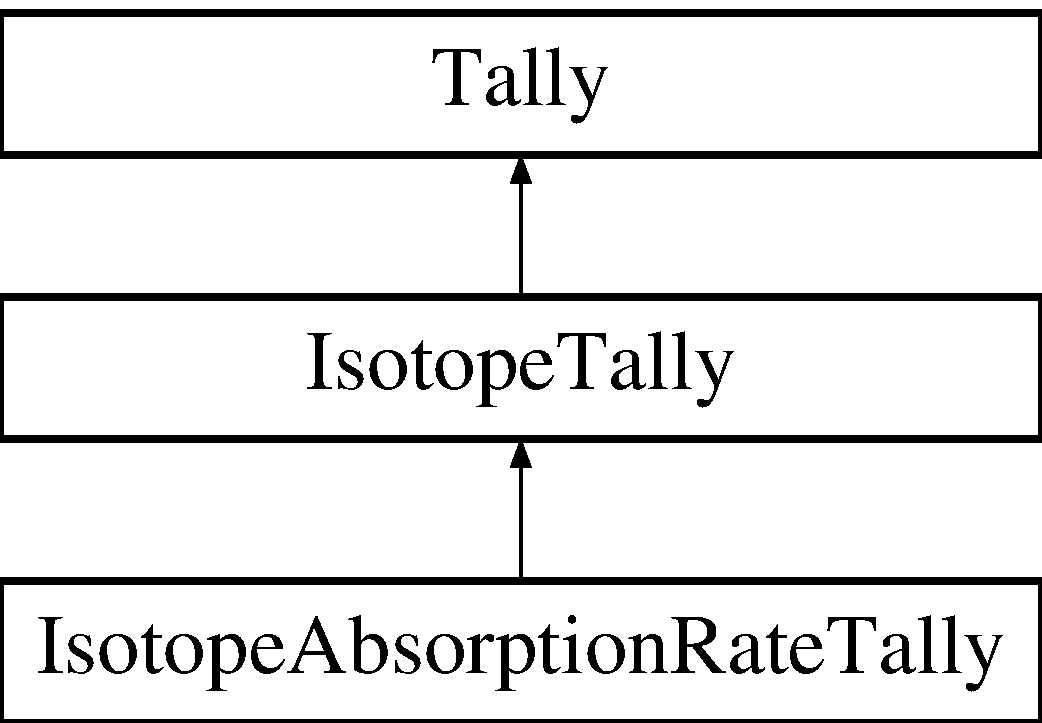
\includegraphics[height=3.000000cm]{classIsotopeAbsorptionRateTally}
\end{center}
\end{figure}
\subsection*{Public Member Functions}
\begin{DoxyCompactItemize}
\item 
\hyperlink{classIsotopeAbsorptionRateTally_a8b88ce947c31e5050a14bf458ae84230}{Isotope\-Absorption\-Rate\-Tally} (\hyperlink{classIsotope}{Isotope} $\ast$isotope, const char $\ast$tally\-\_\-name=(char $\ast$)\char`\"{}\char`\"{})
\begin{DoxyCompactList}\small\item\em \hyperlink{classIsotopeAbsorptionRateTally}{Isotope\-Absorption\-Rate\-Tally} constructor calls the \hyperlink{classIsotopeTally}{Isotope\-Tally} constructor and \hyperlink{classTally}{Tally} constructors and sets the tally type to A\-B\-S\-O\-R\-P\-T\-I\-O\-N\-\_\-\-R\-A\-T\-E. \end{DoxyCompactList}\item 
void \hyperlink{classIsotopeAbsorptionRateTally_a300abb8c8532c790d514700ed2b5e1ee}{tally} (\hyperlink{structneutron}{neutron} $\ast$\hyperlink{structneutron}{neutron})
\begin{DoxyCompactList}\small\item\em \hyperlink{classTally}{Tally} the isotope absorption rate by incrementing the tally by $ \frac{\sigma_a}{\Sigma_t} $ at the neutron's energy. \end{DoxyCompactList}\end{DoxyCompactItemize}
\subsection*{Additional Inherited Members}


\subsection{Detailed Description}
A class for tallying the absorption rate for an isotope. 

\subsection{Constructor \& Destructor Documentation}
\hypertarget{classIsotopeAbsorptionRateTally_a8b88ce947c31e5050a14bf458ae84230}{\index{Isotope\-Absorption\-Rate\-Tally@{Isotope\-Absorption\-Rate\-Tally}!Isotope\-Absorption\-Rate\-Tally@{Isotope\-Absorption\-Rate\-Tally}}
\index{Isotope\-Absorption\-Rate\-Tally@{Isotope\-Absorption\-Rate\-Tally}!IsotopeAbsorptionRateTally@{Isotope\-Absorption\-Rate\-Tally}}
\subsubsection[{Isotope\-Absorption\-Rate\-Tally}]{\setlength{\rightskip}{0pt plus 5cm}Isotope\-Absorption\-Rate\-Tally\-::\-Isotope\-Absorption\-Rate\-Tally (
\begin{DoxyParamCaption}
\item[{{\bf Isotope} $\ast$}]{isotope, }
\item[{const char $\ast$}]{tally\-\_\-name = {\ttfamily (char$\ast$)\char`\"{}\char`\"{}}}
\end{DoxyParamCaption}
)\hspace{0.3cm}{\ttfamily [inline]}}}\label{classIsotopeAbsorptionRateTally_a8b88ce947c31e5050a14bf458ae84230}


\hyperlink{classIsotopeAbsorptionRateTally}{Isotope\-Absorption\-Rate\-Tally} constructor calls the \hyperlink{classIsotopeTally}{Isotope\-Tally} constructor and \hyperlink{classTally}{Tally} constructors and sets the tally type to A\-B\-S\-O\-R\-P\-T\-I\-O\-N\-\_\-\-R\-A\-T\-E. 


\begin{DoxyParams}{Parameters}
{\em isotope} & a pointer to the isotope within which to tally \\
\hline
{\em tally\-\_\-name} & a character array for the tally name (optional) \\
\hline
\end{DoxyParams}


\subsection{Member Function Documentation}
\hypertarget{classIsotopeAbsorptionRateTally_a300abb8c8532c790d514700ed2b5e1ee}{\index{Isotope\-Absorption\-Rate\-Tally@{Isotope\-Absorption\-Rate\-Tally}!tally@{tally}}
\index{tally@{tally}!IsotopeAbsorptionRateTally@{Isotope\-Absorption\-Rate\-Tally}}
\subsubsection[{tally}]{\setlength{\rightskip}{0pt plus 5cm}void Isotope\-Absorption\-Rate\-Tally\-::tally (
\begin{DoxyParamCaption}
\item[{{\bf neutron} $\ast$}]{neutron}
\end{DoxyParamCaption}
)\hspace{0.3cm}{\ttfamily [virtual]}}}\label{classIsotopeAbsorptionRateTally_a300abb8c8532c790d514700ed2b5e1ee}


\hyperlink{classTally}{Tally} the isotope absorption rate by incrementing the tally by $ \frac{\sigma_a}{\Sigma_t} $ at the neutron's energy. 


\begin{DoxyParams}{Parameters}
{\em neutron} & the neutron of interest \\
\hline
\end{DoxyParams}


Implements \hyperlink{classIsotopeTally_a8a5b190e244c630ee7cda35f70287530}{Isotope\-Tally}.



The documentation for this class was generated from the following files\-:\begin{DoxyCompactItemize}
\item 
pinspec/src/\hyperlink{Tally_8h}{Tally.\-h}\item 
pinspec/src/Tally.\-cpp\end{DoxyCompactItemize}

\hypertarget{classIsotopeCaptureRateTally}{\section{Isotope\-Capture\-Rate\-Tally Class Reference}
\label{classIsotopeCaptureRateTally}\index{Isotope\-Capture\-Rate\-Tally@{Isotope\-Capture\-Rate\-Tally}}
}


A class for tallying the capture rate for an isotope.  




{\ttfamily \#include \char`\"{}pinspec/src/\-Tally.\-h\char`\"{}}

Inheritance diagram for Isotope\-Capture\-Rate\-Tally\-:\begin{figure}[H]
\begin{center}
\leavevmode
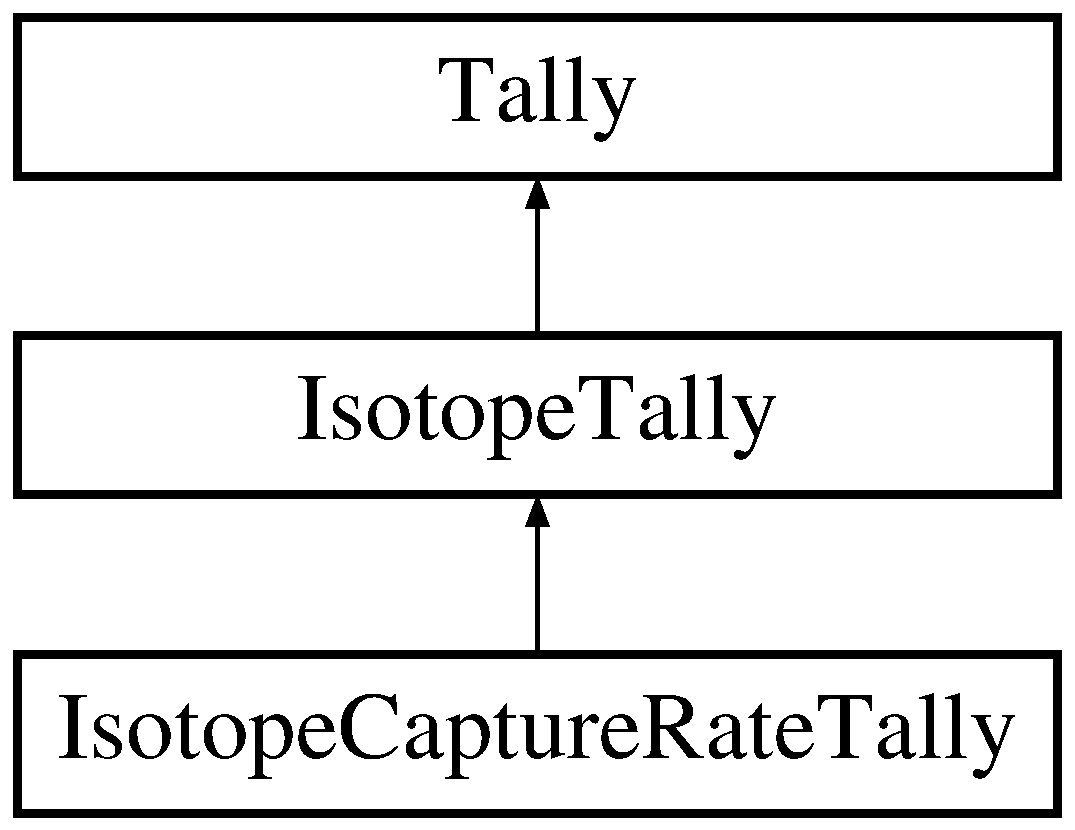
\includegraphics[height=3.000000cm]{classIsotopeCaptureRateTally}
\end{center}
\end{figure}
\subsection*{Public Member Functions}
\begin{DoxyCompactItemize}
\item 
\hyperlink{classIsotopeCaptureRateTally_a2c70af2bf2ba93167f96d1949ded2170}{Isotope\-Capture\-Rate\-Tally} (\hyperlink{classIsotope}{Isotope} $\ast$isotope, const char $\ast$tally\-\_\-name=(char $\ast$)\char`\"{}\char`\"{})
\begin{DoxyCompactList}\small\item\em \hyperlink{classIsotopeCaptureRateTally}{Isotope\-Capture\-Rate\-Tally} constructor calls the \hyperlink{classIsotopeTally}{Isotope\-Tally} constructor and \hyperlink{classTally}{Tally} constructors and sets the tally type to C\-A\-P\-T\-U\-R\-E\-\_\-\-R\-A\-T\-E. \end{DoxyCompactList}\item 
void \hyperlink{classIsotopeCaptureRateTally_a6fb691f21aefd869d86622f6304c05e3}{tally} (\hyperlink{structneutron}{neutron} $\ast$\hyperlink{structneutron}{neutron})
\begin{DoxyCompactList}\small\item\em \hyperlink{classTally}{Tally} the isotope capture rate by incrementing the tally by $ \frac{\sigma_c}{\Sigma_t} $ at the neutron's energy. \end{DoxyCompactList}\end{DoxyCompactItemize}
\subsection*{Additional Inherited Members}


\subsection{Detailed Description}
A class for tallying the capture rate for an isotope. 

\subsection{Constructor \& Destructor Documentation}
\hypertarget{classIsotopeCaptureRateTally_a2c70af2bf2ba93167f96d1949ded2170}{\index{Isotope\-Capture\-Rate\-Tally@{Isotope\-Capture\-Rate\-Tally}!Isotope\-Capture\-Rate\-Tally@{Isotope\-Capture\-Rate\-Tally}}
\index{Isotope\-Capture\-Rate\-Tally@{Isotope\-Capture\-Rate\-Tally}!IsotopeCaptureRateTally@{Isotope\-Capture\-Rate\-Tally}}
\subsubsection[{Isotope\-Capture\-Rate\-Tally}]{\setlength{\rightskip}{0pt plus 5cm}Isotope\-Capture\-Rate\-Tally\-::\-Isotope\-Capture\-Rate\-Tally (
\begin{DoxyParamCaption}
\item[{{\bf Isotope} $\ast$}]{isotope, }
\item[{const char $\ast$}]{tally\-\_\-name = {\ttfamily (char$\ast$)\char`\"{}\char`\"{}}}
\end{DoxyParamCaption}
)\hspace{0.3cm}{\ttfamily [inline]}}}\label{classIsotopeCaptureRateTally_a2c70af2bf2ba93167f96d1949ded2170}


\hyperlink{classIsotopeCaptureRateTally}{Isotope\-Capture\-Rate\-Tally} constructor calls the \hyperlink{classIsotopeTally}{Isotope\-Tally} constructor and \hyperlink{classTally}{Tally} constructors and sets the tally type to C\-A\-P\-T\-U\-R\-E\-\_\-\-R\-A\-T\-E. 


\begin{DoxyParams}{Parameters}
{\em isotope} & a pointer to the isotope within which to tally \\
\hline
{\em tally\-\_\-name} & a character array for the tally name (optional) \\
\hline
\end{DoxyParams}


\subsection{Member Function Documentation}
\hypertarget{classIsotopeCaptureRateTally_a6fb691f21aefd869d86622f6304c05e3}{\index{Isotope\-Capture\-Rate\-Tally@{Isotope\-Capture\-Rate\-Tally}!tally@{tally}}
\index{tally@{tally}!IsotopeCaptureRateTally@{Isotope\-Capture\-Rate\-Tally}}
\subsubsection[{tally}]{\setlength{\rightskip}{0pt plus 5cm}void Isotope\-Capture\-Rate\-Tally\-::tally (
\begin{DoxyParamCaption}
\item[{{\bf neutron} $\ast$}]{neutron}
\end{DoxyParamCaption}
)\hspace{0.3cm}{\ttfamily [virtual]}}}\label{classIsotopeCaptureRateTally_a6fb691f21aefd869d86622f6304c05e3}


\hyperlink{classTally}{Tally} the isotope capture rate by incrementing the tally by $ \frac{\sigma_c}{\Sigma_t} $ at the neutron's energy. 


\begin{DoxyParams}{Parameters}
{\em neutron} & the neutron of interest \\
\hline
\end{DoxyParams}


Implements \hyperlink{classIsotopeTally_a8a5b190e244c630ee7cda35f70287530}{Isotope\-Tally}.



The documentation for this class was generated from the following files\-:\begin{DoxyCompactItemize}
\item 
pinspec/src/\hyperlink{Tally_8h}{Tally.\-h}\item 
pinspec/src/Tally.\-cpp\end{DoxyCompactItemize}

\hypertarget{classIsotopeCollisionRateTally}{\section{Isotope\-Collision\-Rate\-Tally Class Reference}
\label{classIsotopeCollisionRateTally}\index{Isotope\-Collision\-Rate\-Tally@{Isotope\-Collision\-Rate\-Tally}}
}


A class for tallying the collision rate for an isotope.  




{\ttfamily \#include \char`\"{}pinspec/src/\-Tally.\-h\char`\"{}}

Inheritance diagram for Isotope\-Collision\-Rate\-Tally\-:\begin{figure}[H]
\begin{center}
\leavevmode
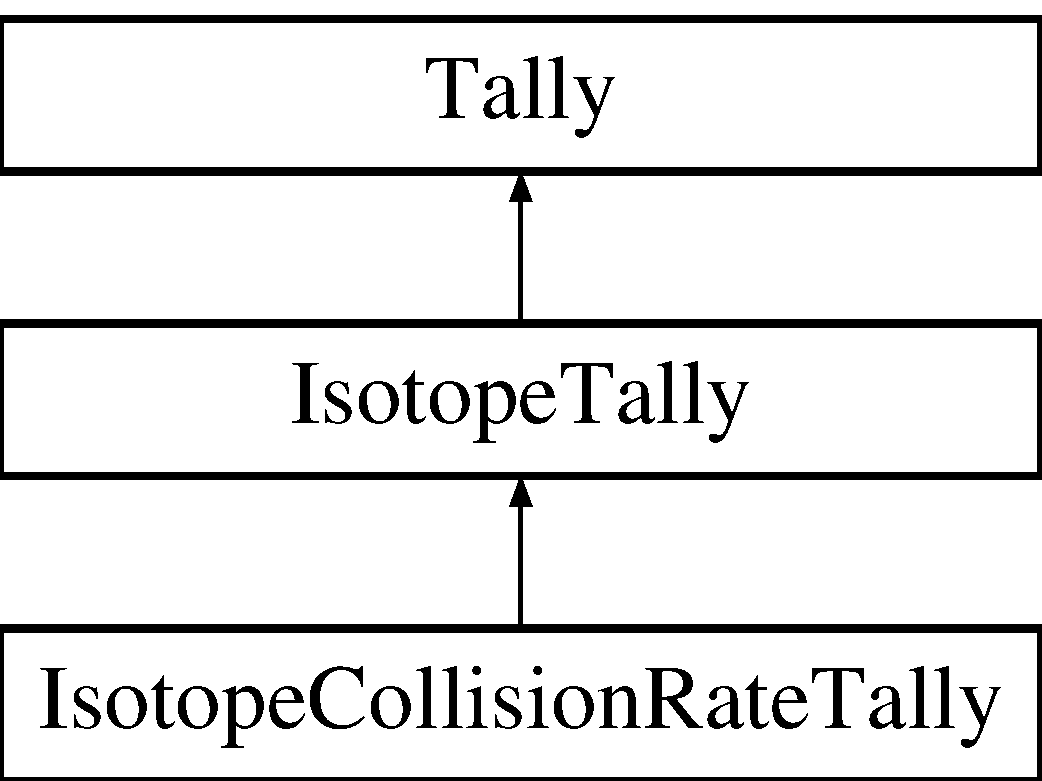
\includegraphics[height=3.000000cm]{classIsotopeCollisionRateTally}
\end{center}
\end{figure}
\subsection*{Public Member Functions}
\begin{DoxyCompactItemize}
\item 
\hyperlink{classIsotopeCollisionRateTally_a4225e720b64ea57595b1295cda742198}{Isotope\-Collision\-Rate\-Tally} (\hyperlink{classIsotope}{Isotope} $\ast$isotope, const char $\ast$tally\-\_\-name=(char $\ast$)\char`\"{}\char`\"{})
\begin{DoxyCompactList}\small\item\em \hyperlink{classIsotopeCollisionRateTally}{Isotope\-Collision\-Rate\-Tally} constructor calls the \hyperlink{classIsotopeTally}{Isotope\-Tally} constructor and \hyperlink{classTally}{Tally} constructors and sets the tally type to C\-O\-L\-L\-I\-S\-I\-O\-N\-\_\-\-R\-A\-T\-E. \end{DoxyCompactList}\item 
void \hyperlink{classIsotopeCollisionRateTally_acd866aa174db9df4b5bdba6347735886}{tally} (\hyperlink{structneutron}{neutron} $\ast$\hyperlink{structneutron}{neutron})
\begin{DoxyCompactList}\small\item\em \hyperlink{classTally}{Tally} the isotope collision rate by incrementing the tally by 1.\-0 at the neutron's energy. \end{DoxyCompactList}\end{DoxyCompactItemize}
\subsection*{Additional Inherited Members}


\subsection{Detailed Description}
A class for tallying the collision rate for an isotope. 

\subsection{Constructor \& Destructor Documentation}
\hypertarget{classIsotopeCollisionRateTally_a4225e720b64ea57595b1295cda742198}{\index{Isotope\-Collision\-Rate\-Tally@{Isotope\-Collision\-Rate\-Tally}!Isotope\-Collision\-Rate\-Tally@{Isotope\-Collision\-Rate\-Tally}}
\index{Isotope\-Collision\-Rate\-Tally@{Isotope\-Collision\-Rate\-Tally}!IsotopeCollisionRateTally@{Isotope\-Collision\-Rate\-Tally}}
\subsubsection[{Isotope\-Collision\-Rate\-Tally}]{\setlength{\rightskip}{0pt plus 5cm}Isotope\-Collision\-Rate\-Tally\-::\-Isotope\-Collision\-Rate\-Tally (
\begin{DoxyParamCaption}
\item[{{\bf Isotope} $\ast$}]{isotope, }
\item[{const char $\ast$}]{tally\-\_\-name = {\ttfamily (char$\ast$)\char`\"{}\char`\"{}}}
\end{DoxyParamCaption}
)\hspace{0.3cm}{\ttfamily [inline]}}}\label{classIsotopeCollisionRateTally_a4225e720b64ea57595b1295cda742198}


\hyperlink{classIsotopeCollisionRateTally}{Isotope\-Collision\-Rate\-Tally} constructor calls the \hyperlink{classIsotopeTally}{Isotope\-Tally} constructor and \hyperlink{classTally}{Tally} constructors and sets the tally type to C\-O\-L\-L\-I\-S\-I\-O\-N\-\_\-\-R\-A\-T\-E. 


\begin{DoxyParams}{Parameters}
{\em isotope} & a pointer to the isotope within which to tally \\
\hline
{\em tally\-\_\-name} & a character array for the tally name (optional) \\
\hline
\end{DoxyParams}


\subsection{Member Function Documentation}
\hypertarget{classIsotopeCollisionRateTally_acd866aa174db9df4b5bdba6347735886}{\index{Isotope\-Collision\-Rate\-Tally@{Isotope\-Collision\-Rate\-Tally}!tally@{tally}}
\index{tally@{tally}!IsotopeCollisionRateTally@{Isotope\-Collision\-Rate\-Tally}}
\subsubsection[{tally}]{\setlength{\rightskip}{0pt plus 5cm}void Isotope\-Collision\-Rate\-Tally\-::tally (
\begin{DoxyParamCaption}
\item[{{\bf neutron} $\ast$}]{neutron}
\end{DoxyParamCaption}
)\hspace{0.3cm}{\ttfamily [virtual]}}}\label{classIsotopeCollisionRateTally_acd866aa174db9df4b5bdba6347735886}


\hyperlink{classTally}{Tally} the isotope collision rate by incrementing the tally by 1.\-0 at the neutron's energy. 


\begin{DoxyParams}{Parameters}
{\em neutron} & the neutron of interest \\
\hline
\end{DoxyParams}


Implements \hyperlink{classIsotopeTally_a8a5b190e244c630ee7cda35f70287530}{Isotope\-Tally}.



The documentation for this class was generated from the following files\-:\begin{DoxyCompactItemize}
\item 
pinspec/src/\hyperlink{Tally_8h}{Tally.\-h}\item 
pinspec/src/Tally.\-cpp\end{DoxyCompactItemize}

\hypertarget{classIsotopeDiffusionRateTally}{\section{Isotope\-Diffusion\-Rate\-Tally Class Reference}
\label{classIsotopeDiffusionRateTally}\index{Isotope\-Diffusion\-Rate\-Tally@{Isotope\-Diffusion\-Rate\-Tally}}
}


A class for tallying the diffusion rate for an isotope.  




{\ttfamily \#include \char`\"{}pinspec/src/\-Tally.\-h\char`\"{}}

Inheritance diagram for Isotope\-Diffusion\-Rate\-Tally\-:\begin{figure}[H]
\begin{center}
\leavevmode
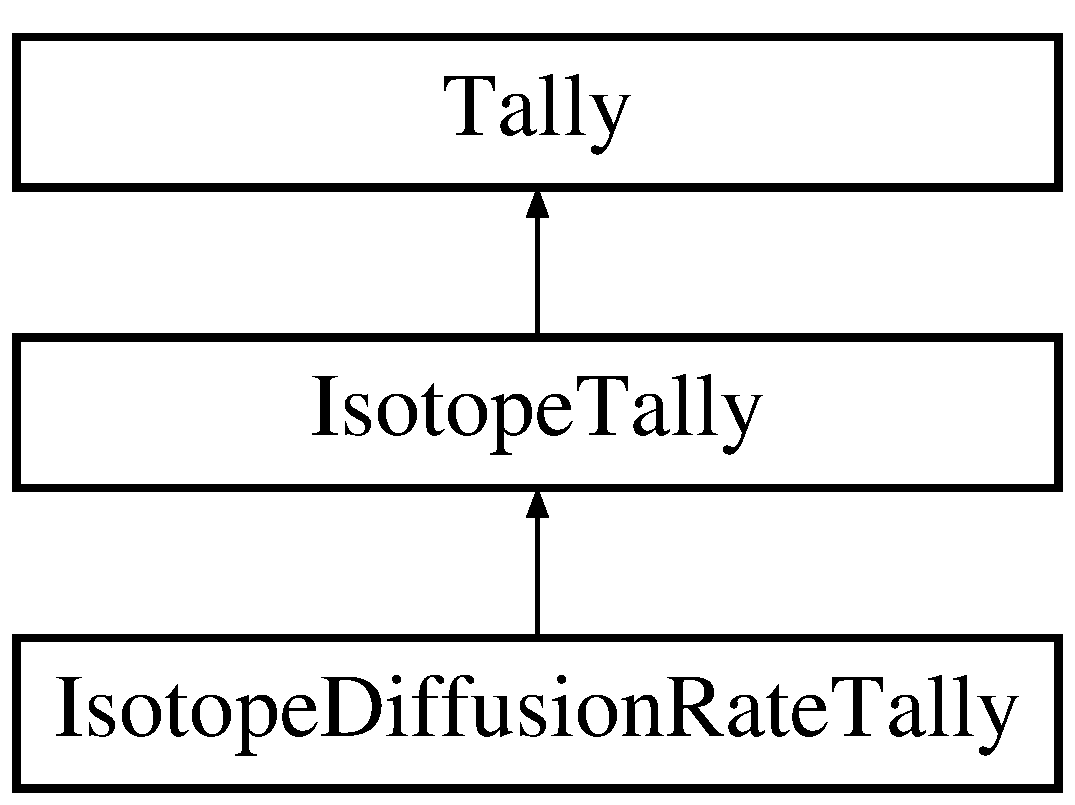
\includegraphics[height=3.000000cm]{classIsotopeDiffusionRateTally}
\end{center}
\end{figure}
\subsection*{Public Member Functions}
\begin{DoxyCompactItemize}
\item 
\hyperlink{classIsotopeDiffusionRateTally_af7261cada71cb0cea0a6f3f4d5b92f4c}{Isotope\-Diffusion\-Rate\-Tally} (\hyperlink{classIsotope}{Isotope} $\ast$isotope, const char $\ast$tally\-\_\-name=(char $\ast$)\char`\"{}\char`\"{})
\begin{DoxyCompactList}\small\item\em \hyperlink{classIsotopeDiffusionRateTally}{Isotope\-Diffusion\-Rate\-Tally} constructor calls the \hyperlink{classIsotopeTally}{Isotope\-Tally} constructor and \hyperlink{classTally}{Tally} constructors and sets the tally type to D\-I\-F\-F\-U\-S\-I\-O\-N\-\_\-\-R\-A\-T\-E. \end{DoxyCompactList}\item 
void \hyperlink{classIsotopeDiffusionRateTally_af9de72dec40388388faba7fdf13ec5a4}{tally} (\hyperlink{structneutron}{neutron} $\ast$\hyperlink{structneutron}{neutron})
\begin{DoxyCompactList}\small\item\em \hyperlink{classTally}{Tally} the isotope diffusion rate by incrementing the tally by $ \frac{\frac{1}{3\sigma_tr}}{\Sigma_t} $ at the neutron's energy. \end{DoxyCompactList}\end{DoxyCompactItemize}
\subsection*{Additional Inherited Members}


\subsection{Detailed Description}
A class for tallying the diffusion rate for an isotope. 

\subsection{Constructor \& Destructor Documentation}
\hypertarget{classIsotopeDiffusionRateTally_af7261cada71cb0cea0a6f3f4d5b92f4c}{\index{Isotope\-Diffusion\-Rate\-Tally@{Isotope\-Diffusion\-Rate\-Tally}!Isotope\-Diffusion\-Rate\-Tally@{Isotope\-Diffusion\-Rate\-Tally}}
\index{Isotope\-Diffusion\-Rate\-Tally@{Isotope\-Diffusion\-Rate\-Tally}!IsotopeDiffusionRateTally@{Isotope\-Diffusion\-Rate\-Tally}}
\subsubsection[{Isotope\-Diffusion\-Rate\-Tally}]{\setlength{\rightskip}{0pt plus 5cm}Isotope\-Diffusion\-Rate\-Tally\-::\-Isotope\-Diffusion\-Rate\-Tally (
\begin{DoxyParamCaption}
\item[{{\bf Isotope} $\ast$}]{isotope, }
\item[{const char $\ast$}]{tally\-\_\-name = {\ttfamily (char$\ast$)\char`\"{}\char`\"{}}}
\end{DoxyParamCaption}
)\hspace{0.3cm}{\ttfamily [inline]}}}\label{classIsotopeDiffusionRateTally_af7261cada71cb0cea0a6f3f4d5b92f4c}


\hyperlink{classIsotopeDiffusionRateTally}{Isotope\-Diffusion\-Rate\-Tally} constructor calls the \hyperlink{classIsotopeTally}{Isotope\-Tally} constructor and \hyperlink{classTally}{Tally} constructors and sets the tally type to D\-I\-F\-F\-U\-S\-I\-O\-N\-\_\-\-R\-A\-T\-E. 


\begin{DoxyParams}{Parameters}
{\em isotope} & a pointer to the isotope within which to tally \\
\hline
{\em tally\-\_\-name} & a character array for the tally name (optional) \\
\hline
\end{DoxyParams}


\subsection{Member Function Documentation}
\hypertarget{classIsotopeDiffusionRateTally_af9de72dec40388388faba7fdf13ec5a4}{\index{Isotope\-Diffusion\-Rate\-Tally@{Isotope\-Diffusion\-Rate\-Tally}!tally@{tally}}
\index{tally@{tally}!IsotopeDiffusionRateTally@{Isotope\-Diffusion\-Rate\-Tally}}
\subsubsection[{tally}]{\setlength{\rightskip}{0pt plus 5cm}void Isotope\-Diffusion\-Rate\-Tally\-::tally (
\begin{DoxyParamCaption}
\item[{{\bf neutron} $\ast$}]{neutron}
\end{DoxyParamCaption}
)\hspace{0.3cm}{\ttfamily [virtual]}}}\label{classIsotopeDiffusionRateTally_af9de72dec40388388faba7fdf13ec5a4}


\hyperlink{classTally}{Tally} the isotope diffusion rate by incrementing the tally by $ \frac{\frac{1}{3\sigma_tr}}{\Sigma_t} $ at the neutron's energy. 


\begin{DoxyParams}{Parameters}
{\em neutron} & the neutron of interest \\
\hline
\end{DoxyParams}


Implements \hyperlink{classIsotopeTally_a8a5b190e244c630ee7cda35f70287530}{Isotope\-Tally}.



The documentation for this class was generated from the following files\-:\begin{DoxyCompactItemize}
\item 
pinspec/src/\hyperlink{Tally_8h}{Tally.\-h}\item 
pinspec/src/Tally.\-cpp\end{DoxyCompactItemize}

\hypertarget{classIsotopeElasticRateTally}{\section{Isotope\-Elastic\-Rate\-Tally Class Reference}
\label{classIsotopeElasticRateTally}\index{Isotope\-Elastic\-Rate\-Tally@{Isotope\-Elastic\-Rate\-Tally}}
}


A class for tallying the elastic scattering rate for an isotope.  




{\ttfamily \#include \char`\"{}pinspec/src/\-Tally.\-h\char`\"{}}

Inheritance diagram for Isotope\-Elastic\-Rate\-Tally\-:\begin{figure}[H]
\begin{center}
\leavevmode
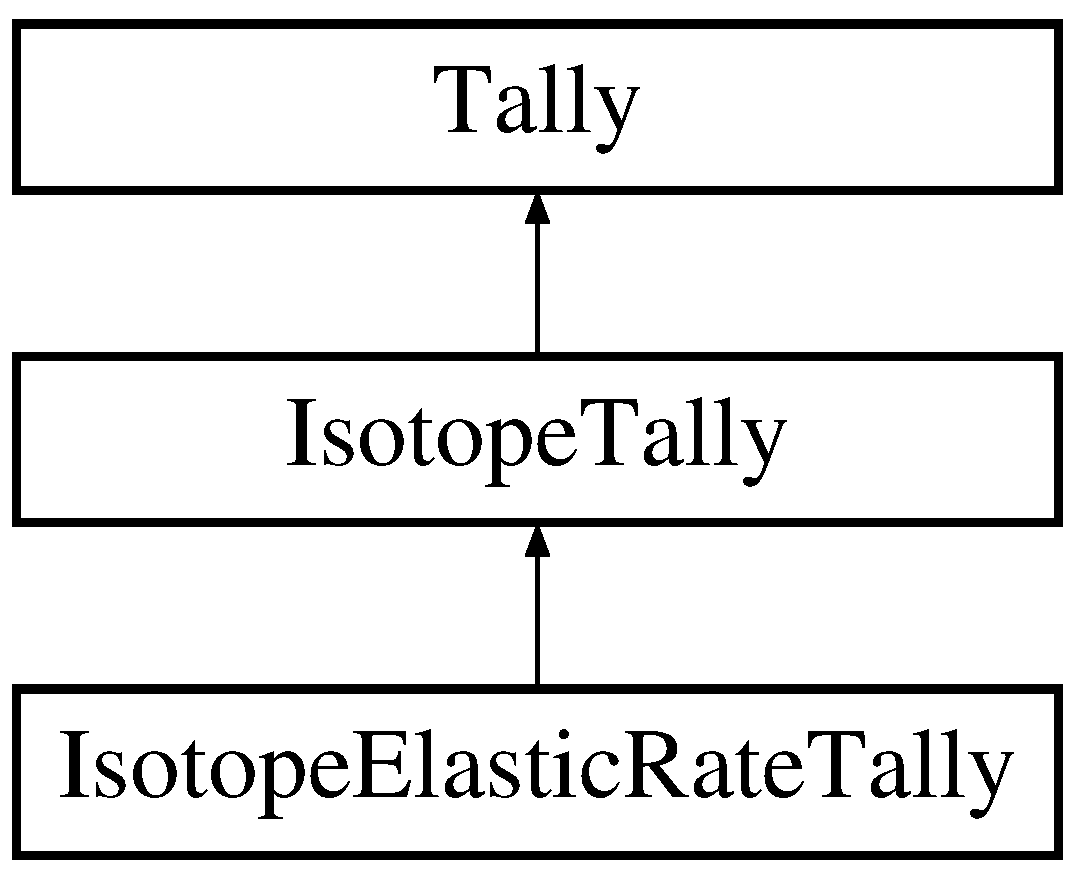
\includegraphics[height=3.000000cm]{classIsotopeElasticRateTally}
\end{center}
\end{figure}
\subsection*{Public Member Functions}
\begin{DoxyCompactItemize}
\item 
\hyperlink{classIsotopeElasticRateTally_a4f590fce6ac4136240fb5ddadfbcc3c0}{Isotope\-Elastic\-Rate\-Tally} (\hyperlink{classIsotope}{Isotope} $\ast$isotope, const char $\ast$tally\-\_\-name=(char $\ast$)\char`\"{}\char`\"{})
\begin{DoxyCompactList}\small\item\em \hyperlink{classIsotopeElasticRateTally}{Isotope\-Elastic\-Rate\-Tally} constructor calls the \hyperlink{classIsotopeTally}{Isotope\-Tally} constructor and \hyperlink{classTally}{Tally} constructors and sets the tally type to E\-L\-A\-S\-T\-I\-C\-\_\-\-R\-A\-T\-E. \end{DoxyCompactList}\item 
void \hyperlink{classIsotopeElasticRateTally_a641673a78be89eec1f1be4d424f0e078}{tally} (\hyperlink{structneutron}{neutron} $\ast$\hyperlink{structneutron}{neutron})
\begin{DoxyCompactList}\small\item\em \hyperlink{classTally}{Tally} the isotope elastic scattering rate by incrementing the tally by $ \frac{\sigma_s}{\Sigma_t} $ at the neutron's energy. \end{DoxyCompactList}\end{DoxyCompactItemize}
\subsection*{Additional Inherited Members}


\subsection{Detailed Description}
A class for tallying the elastic scattering rate for an isotope. 

\subsection{Constructor \& Destructor Documentation}
\hypertarget{classIsotopeElasticRateTally_a4f590fce6ac4136240fb5ddadfbcc3c0}{\index{Isotope\-Elastic\-Rate\-Tally@{Isotope\-Elastic\-Rate\-Tally}!Isotope\-Elastic\-Rate\-Tally@{Isotope\-Elastic\-Rate\-Tally}}
\index{Isotope\-Elastic\-Rate\-Tally@{Isotope\-Elastic\-Rate\-Tally}!IsotopeElasticRateTally@{Isotope\-Elastic\-Rate\-Tally}}
\subsubsection[{Isotope\-Elastic\-Rate\-Tally}]{\setlength{\rightskip}{0pt plus 5cm}Isotope\-Elastic\-Rate\-Tally\-::\-Isotope\-Elastic\-Rate\-Tally (
\begin{DoxyParamCaption}
\item[{{\bf Isotope} $\ast$}]{isotope, }
\item[{const char $\ast$}]{tally\-\_\-name = {\ttfamily (char$\ast$)\char`\"{}\char`\"{}}}
\end{DoxyParamCaption}
)\hspace{0.3cm}{\ttfamily [inline]}}}\label{classIsotopeElasticRateTally_a4f590fce6ac4136240fb5ddadfbcc3c0}


\hyperlink{classIsotopeElasticRateTally}{Isotope\-Elastic\-Rate\-Tally} constructor calls the \hyperlink{classIsotopeTally}{Isotope\-Tally} constructor and \hyperlink{classTally}{Tally} constructors and sets the tally type to E\-L\-A\-S\-T\-I\-C\-\_\-\-R\-A\-T\-E. 


\begin{DoxyParams}{Parameters}
{\em isotope} & a pointer to the isotope for which to tally \\
\hline
{\em tally\-\_\-name} & a character array for the tally name (optional) \\
\hline
\end{DoxyParams}


\subsection{Member Function Documentation}
\hypertarget{classIsotopeElasticRateTally_a641673a78be89eec1f1be4d424f0e078}{\index{Isotope\-Elastic\-Rate\-Tally@{Isotope\-Elastic\-Rate\-Tally}!tally@{tally}}
\index{tally@{tally}!IsotopeElasticRateTally@{Isotope\-Elastic\-Rate\-Tally}}
\subsubsection[{tally}]{\setlength{\rightskip}{0pt plus 5cm}void Isotope\-Elastic\-Rate\-Tally\-::tally (
\begin{DoxyParamCaption}
\item[{{\bf neutron} $\ast$}]{neutron}
\end{DoxyParamCaption}
)\hspace{0.3cm}{\ttfamily [virtual]}}}\label{classIsotopeElasticRateTally_a641673a78be89eec1f1be4d424f0e078}


\hyperlink{classTally}{Tally} the isotope elastic scattering rate by incrementing the tally by $ \frac{\sigma_s}{\Sigma_t} $ at the neutron's energy. 


\begin{DoxyParams}{Parameters}
{\em neutron} & the neutron of interest \\
\hline
\end{DoxyParams}


Implements \hyperlink{classIsotopeTally_a8a5b190e244c630ee7cda35f70287530}{Isotope\-Tally}.



The documentation for this class was generated from the following files\-:\begin{DoxyCompactItemize}
\item 
pinspec/src/\hyperlink{Tally_8h}{Tally.\-h}\item 
pinspec/src/Tally.\-cpp\end{DoxyCompactItemize}

\hypertarget{classIsotopeFissionRateTally}{\section{Isotope\-Fission\-Rate\-Tally Class Reference}
\label{classIsotopeFissionRateTally}\index{Isotope\-Fission\-Rate\-Tally@{Isotope\-Fission\-Rate\-Tally}}
}


A class for tallying the fission rate for an isotope.  




{\ttfamily \#include \char`\"{}pinspec/src/\-Tally.\-h\char`\"{}}

Inheritance diagram for Isotope\-Fission\-Rate\-Tally\-:\begin{figure}[H]
\begin{center}
\leavevmode
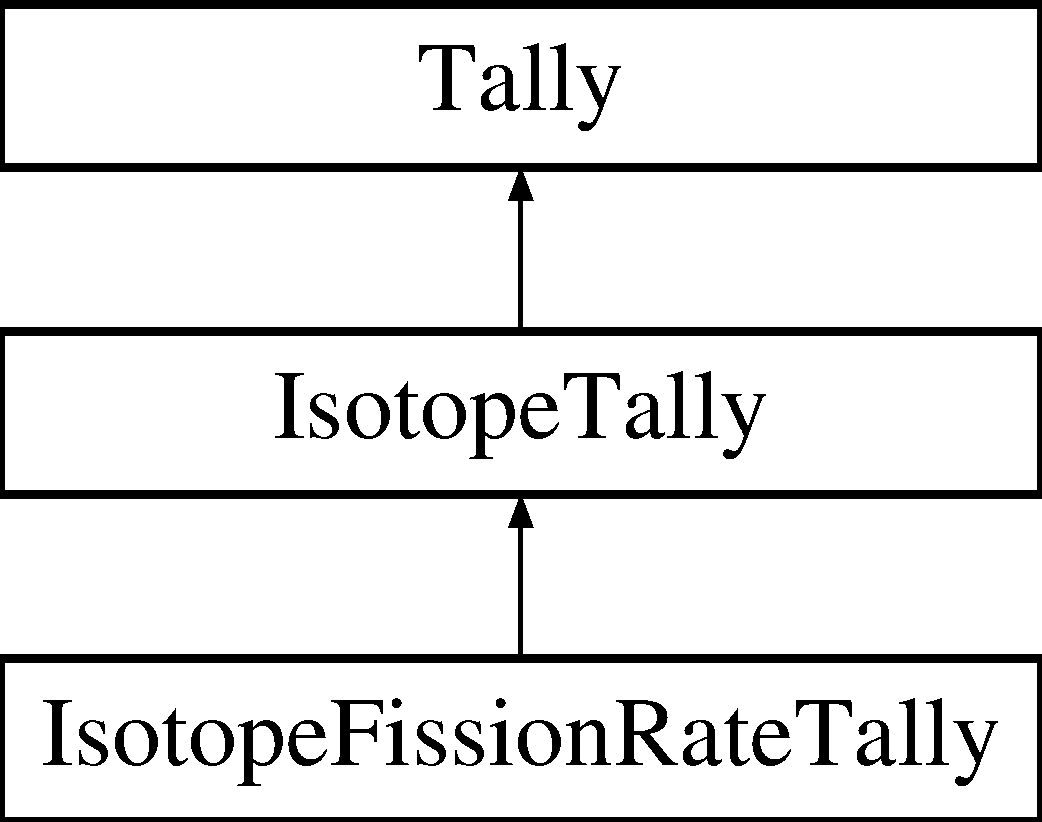
\includegraphics[height=3.000000cm]{classIsotopeFissionRateTally}
\end{center}
\end{figure}
\subsection*{Public Member Functions}
\begin{DoxyCompactItemize}
\item 
\hyperlink{classIsotopeFissionRateTally_a3fc1712cbad1343b8580560e152442c1}{Isotope\-Fission\-Rate\-Tally} (\hyperlink{classIsotope}{Isotope} $\ast$isotope, const char $\ast$tally\-\_\-name=(char $\ast$)\char`\"{}\char`\"{})
\begin{DoxyCompactList}\small\item\em \hyperlink{classIsotopeFissionRateTally}{Isotope\-Fission\-Rate\-Tally} constructor calls the \hyperlink{classIsotopeTally}{Isotope\-Tally} constructor and \hyperlink{classTally}{Tally} constructors and sets the tally type to F\-I\-S\-S\-I\-O\-N\-\_\-\-R\-A\-T\-E. \end{DoxyCompactList}\item 
void \hyperlink{classIsotopeFissionRateTally_aeeed9917e1134a1a37ed58a5f94dd569}{tally} (\hyperlink{structneutron}{neutron} $\ast$\hyperlink{structneutron}{neutron})
\begin{DoxyCompactList}\small\item\em \hyperlink{classTally}{Tally} the isotope fission rate by incrementing the tally by $ \frac{\sigma_f}{\Sigma_t} $ at the neutron's energy. \end{DoxyCompactList}\end{DoxyCompactItemize}
\subsection*{Additional Inherited Members}


\subsection{Detailed Description}
A class for tallying the fission rate for an isotope. 

\subsection{Constructor \& Destructor Documentation}
\hypertarget{classIsotopeFissionRateTally_a3fc1712cbad1343b8580560e152442c1}{\index{Isotope\-Fission\-Rate\-Tally@{Isotope\-Fission\-Rate\-Tally}!Isotope\-Fission\-Rate\-Tally@{Isotope\-Fission\-Rate\-Tally}}
\index{Isotope\-Fission\-Rate\-Tally@{Isotope\-Fission\-Rate\-Tally}!IsotopeFissionRateTally@{Isotope\-Fission\-Rate\-Tally}}
\subsubsection[{Isotope\-Fission\-Rate\-Tally}]{\setlength{\rightskip}{0pt plus 5cm}Isotope\-Fission\-Rate\-Tally\-::\-Isotope\-Fission\-Rate\-Tally (
\begin{DoxyParamCaption}
\item[{{\bf Isotope} $\ast$}]{isotope, }
\item[{const char $\ast$}]{tally\-\_\-name = {\ttfamily (char$\ast$)\char`\"{}\char`\"{}}}
\end{DoxyParamCaption}
)\hspace{0.3cm}{\ttfamily [inline]}}}\label{classIsotopeFissionRateTally_a3fc1712cbad1343b8580560e152442c1}


\hyperlink{classIsotopeFissionRateTally}{Isotope\-Fission\-Rate\-Tally} constructor calls the \hyperlink{classIsotopeTally}{Isotope\-Tally} constructor and \hyperlink{classTally}{Tally} constructors and sets the tally type to F\-I\-S\-S\-I\-O\-N\-\_\-\-R\-A\-T\-E. 


\begin{DoxyParams}{Parameters}
{\em isotope} & a pointer to the isotope within which to tally \\
\hline
{\em tally\-\_\-name} & a character array for the tally name (optional) \\
\hline
\end{DoxyParams}


\subsection{Member Function Documentation}
\hypertarget{classIsotopeFissionRateTally_aeeed9917e1134a1a37ed58a5f94dd569}{\index{Isotope\-Fission\-Rate\-Tally@{Isotope\-Fission\-Rate\-Tally}!tally@{tally}}
\index{tally@{tally}!IsotopeFissionRateTally@{Isotope\-Fission\-Rate\-Tally}}
\subsubsection[{tally}]{\setlength{\rightskip}{0pt plus 5cm}void Isotope\-Fission\-Rate\-Tally\-::tally (
\begin{DoxyParamCaption}
\item[{{\bf neutron} $\ast$}]{neutron}
\end{DoxyParamCaption}
)\hspace{0.3cm}{\ttfamily [virtual]}}}\label{classIsotopeFissionRateTally_aeeed9917e1134a1a37ed58a5f94dd569}


\hyperlink{classTally}{Tally} the isotope fission rate by incrementing the tally by $ \frac{\sigma_f}{\Sigma_t} $ at the neutron's energy. 


\begin{DoxyParams}{Parameters}
{\em neutron} & the neutron of interest \\
\hline
\end{DoxyParams}


Implements \hyperlink{classIsotopeTally_a8a5b190e244c630ee7cda35f70287530}{Isotope\-Tally}.



The documentation for this class was generated from the following files\-:\begin{DoxyCompactItemize}
\item 
\hyperlink{Tally_8h}{Tally.\-h}\item 
Tally.\-cpp\end{DoxyCompactItemize}

\hypertarget{classIsotopeTally}{\section{Isotope\-Tally Class Reference}
\label{classIsotopeTally}\index{Isotope\-Tally@{Isotope\-Tally}}
}


An abstract class for tallies with I\-S\-O\-T\-O\-P\-E domain type.  




{\ttfamily \#include \char`\"{}pinspec/src/\-Tally.\-h\char`\"{}}

Inheritance diagram for Isotope\-Tally\-:\begin{figure}[H]
\begin{center}
\leavevmode
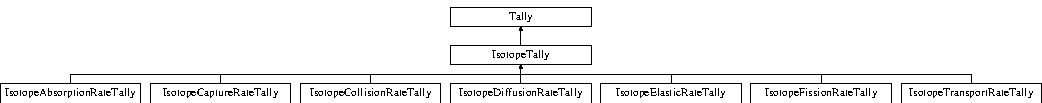
\includegraphics[height=1.387283cm]{classIsotopeTally}
\end{center}
\end{figure}
\subsection*{Public Member Functions}
\begin{DoxyCompactItemize}
\item 
\hyperlink{classIsotopeTally_a99b6c5ff93bcab9176d9cd7bc561617e}{Isotope\-Tally} (\hyperlink{classIsotope}{Isotope} $\ast$isotope, const char $\ast$tally\-\_\-name=(char $\ast$)\char`\"{}\char`\"{})
\begin{DoxyCompactList}\small\item\em \hyperlink{classIsotopeTally}{Isotope\-Tally} constructor calls the \hyperlink{classTally}{Tally} constructor and sets the tally domain to I\-S\-O\-T\-O\-P\-E. \end{DoxyCompactList}\item 
\hyperlink{classIsotope}{Isotope} $\ast$ \hyperlink{classIsotopeTally_a7dbed38017c97998a9f3bd1560ecf750}{get\-Isotope} ()
\begin{DoxyCompactList}\small\item\em Returns the isotope for this tally. \end{DoxyCompactList}\item 
\hypertarget{classIsotopeTally_a8a5b190e244c630ee7cda35f70287530}{virtual void \hyperlink{classIsotopeTally_a8a5b190e244c630ee7cda35f70287530}{tally} (\hyperlink{structneutron}{neutron} $\ast$\hyperlink{structneutron}{neutron})=0}\label{classIsotopeTally_a8a5b190e244c630ee7cda35f70287530}

\begin{DoxyCompactList}\small\item\em A method to tally a neutron to be implemented by subclasses. \end{DoxyCompactList}\end{DoxyCompactItemize}
\subsection*{Protected Attributes}
\begin{DoxyCompactItemize}
\item 
\hyperlink{classIsotope}{Isotope} $\ast$ \hyperlink{classIsotopeTally_a18a3c41c4553300828f2e7f51496adf0}{\-\_\-isotope}
\end{DoxyCompactItemize}


\subsection{Detailed Description}
An abstract class for tallies with I\-S\-O\-T\-O\-P\-E domain type. 

An \hyperlink{classIsotopeTally}{Isotope\-Tally} is for tallying a specific reaction rate for an isotope within a material, region or the geometry. \hyperlink{classIsotope}{Isotope} tallies are especially useful for computing resonance integrals. The \hyperlink{classIsotopeTally}{Isotope\-Tally} is an abstract class and must be implemented for each tally\-Type. 

\subsection{Constructor \& Destructor Documentation}
\hypertarget{classIsotopeTally_a99b6c5ff93bcab9176d9cd7bc561617e}{\index{Isotope\-Tally@{Isotope\-Tally}!Isotope\-Tally@{Isotope\-Tally}}
\index{Isotope\-Tally@{Isotope\-Tally}!IsotopeTally@{Isotope\-Tally}}
\subsubsection[{Isotope\-Tally}]{\setlength{\rightskip}{0pt plus 5cm}Isotope\-Tally\-::\-Isotope\-Tally (
\begin{DoxyParamCaption}
\item[{{\bf Isotope} $\ast$}]{isotope, }
\item[{const char $\ast$}]{tally\-\_\-name = {\ttfamily (char$\ast$)\char`\"{}\char`\"{}}}
\end{DoxyParamCaption}
)\hspace{0.3cm}{\ttfamily [inline]}}}\label{classIsotopeTally_a99b6c5ff93bcab9176d9cd7bc561617e}


\hyperlink{classIsotopeTally}{Isotope\-Tally} constructor calls the \hyperlink{classTally}{Tally} constructor and sets the tally domain to I\-S\-O\-T\-O\-P\-E. 


\begin{DoxyParams}{Parameters}
{\em isotope} & a pointer to the isotope to tally \\
\hline
{\em tally\-\_\-name} & a character array for the tally name (optional) \\
\hline
\end{DoxyParams}


\subsection{Member Function Documentation}
\hypertarget{classIsotopeTally_a7dbed38017c97998a9f3bd1560ecf750}{\index{Isotope\-Tally@{Isotope\-Tally}!get\-Isotope@{get\-Isotope}}
\index{get\-Isotope@{get\-Isotope}!IsotopeTally@{Isotope\-Tally}}
\subsubsection[{get\-Isotope}]{\setlength{\rightskip}{0pt plus 5cm}{\bf Isotope}$\ast$ Isotope\-Tally\-::get\-Isotope (
\begin{DoxyParamCaption}
{}
\end{DoxyParamCaption}
)\hspace{0.3cm}{\ttfamily [inline]}}}\label{classIsotopeTally_a7dbed38017c97998a9f3bd1560ecf750}


Returns the isotope for this tally. 

\begin{DoxyReturn}{Returns}
a pointer to the isotope 
\end{DoxyReturn}


\subsection{Member Data Documentation}
\hypertarget{classIsotopeTally_a18a3c41c4553300828f2e7f51496adf0}{\index{Isotope\-Tally@{Isotope\-Tally}!\-\_\-isotope@{\-\_\-isotope}}
\index{\-\_\-isotope@{\-\_\-isotope}!IsotopeTally@{Isotope\-Tally}}
\subsubsection[{\-\_\-isotope}]{\setlength{\rightskip}{0pt plus 5cm}{\bf Isotope}$\ast$ Isotope\-Tally\-::\-\_\-isotope\hspace{0.3cm}{\ttfamily [protected]}}}\label{classIsotopeTally_a18a3c41c4553300828f2e7f51496adf0}
A pointer to the isotope for this tally 

The documentation for this class was generated from the following file\-:\begin{DoxyCompactItemize}
\item 
pinspec/src/\hyperlink{Tally_8h}{Tally.\-h}\end{DoxyCompactItemize}

\hypertarget{classIsotopeTransportRateTally}{\section{Isotope\-Transport\-Rate\-Tally Class Reference}
\label{classIsotopeTransportRateTally}\index{Isotope\-Transport\-Rate\-Tally@{Isotope\-Transport\-Rate\-Tally}}
}


A class for tallying the transport rate for an isotope.  




{\ttfamily \#include \char`\"{}pinspec/src/\-Tally.\-h\char`\"{}}

Inheritance diagram for Isotope\-Transport\-Rate\-Tally\-:\begin{figure}[H]
\begin{center}
\leavevmode
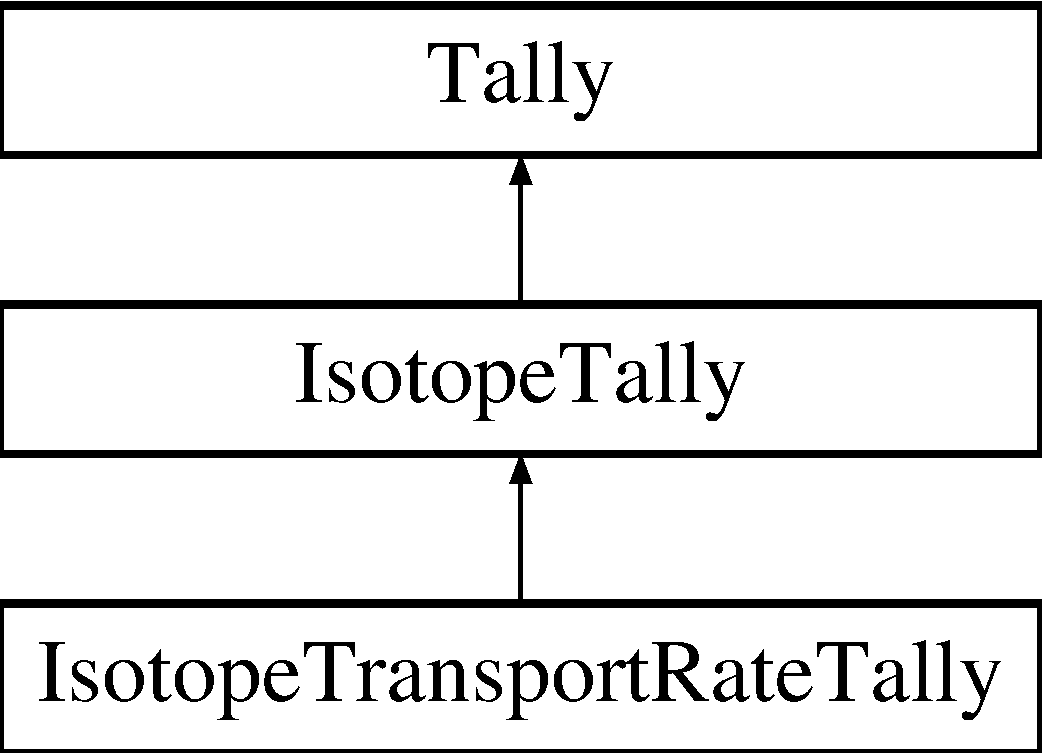
\includegraphics[height=3.000000cm]{classIsotopeTransportRateTally}
\end{center}
\end{figure}
\subsection*{Public Member Functions}
\begin{DoxyCompactItemize}
\item 
\hyperlink{classIsotopeTransportRateTally_a80842d6877d46b24bc02f88e884c5e1d}{Isotope\-Transport\-Rate\-Tally} (\hyperlink{classIsotope}{Isotope} $\ast$isotope, const char $\ast$tally\-\_\-name=(char $\ast$)\char`\"{}\char`\"{})
\begin{DoxyCompactList}\small\item\em \hyperlink{classIsotopeTransportRateTally}{Isotope\-Transport\-Rate\-Tally} constructor calls the \hyperlink{classIsotopeTally}{Isotope\-Tally} constructor and \hyperlink{classTally}{Tally} constructors and sets the tally type to T\-R\-A\-N\-S\-P\-O\-R\-T\-\_\-\-R\-A\-T\-E. \end{DoxyCompactList}\item 
void \hyperlink{classIsotopeTransportRateTally_a5a747ab9d3704757ff9ec585fa402e84}{tally} (\hyperlink{structneutron}{neutron} $\ast$\hyperlink{structneutron}{neutron})
\begin{DoxyCompactList}\small\item\em \hyperlink{classTally}{Tally} the isotope transport rate by incrementing the tally by $ \frac{\sigma_tr}{\Sigma_t} $ at the neutron's energy. \end{DoxyCompactList}\end{DoxyCompactItemize}
\subsection*{Additional Inherited Members}


\subsection{Detailed Description}
A class for tallying the transport rate for an isotope. 

\subsection{Constructor \& Destructor Documentation}
\hypertarget{classIsotopeTransportRateTally_a80842d6877d46b24bc02f88e884c5e1d}{\index{Isotope\-Transport\-Rate\-Tally@{Isotope\-Transport\-Rate\-Tally}!Isotope\-Transport\-Rate\-Tally@{Isotope\-Transport\-Rate\-Tally}}
\index{Isotope\-Transport\-Rate\-Tally@{Isotope\-Transport\-Rate\-Tally}!IsotopeTransportRateTally@{Isotope\-Transport\-Rate\-Tally}}
\subsubsection[{Isotope\-Transport\-Rate\-Tally}]{\setlength{\rightskip}{0pt plus 5cm}Isotope\-Transport\-Rate\-Tally\-::\-Isotope\-Transport\-Rate\-Tally (
\begin{DoxyParamCaption}
\item[{{\bf Isotope} $\ast$}]{isotope, }
\item[{const char $\ast$}]{tally\-\_\-name = {\ttfamily (char$\ast$)\char`\"{}\char`\"{}}}
\end{DoxyParamCaption}
)\hspace{0.3cm}{\ttfamily [inline]}}}\label{classIsotopeTransportRateTally_a80842d6877d46b24bc02f88e884c5e1d}


\hyperlink{classIsotopeTransportRateTally}{Isotope\-Transport\-Rate\-Tally} constructor calls the \hyperlink{classIsotopeTally}{Isotope\-Tally} constructor and \hyperlink{classTally}{Tally} constructors and sets the tally type to T\-R\-A\-N\-S\-P\-O\-R\-T\-\_\-\-R\-A\-T\-E. 


\begin{DoxyParams}{Parameters}
{\em isotope} & a pointer to the isotope within which to tally \\
\hline
{\em tally\-\_\-name} & a character array for the tally name (optional) \\
\hline
\end{DoxyParams}


\subsection{Member Function Documentation}
\hypertarget{classIsotopeTransportRateTally_a5a747ab9d3704757ff9ec585fa402e84}{\index{Isotope\-Transport\-Rate\-Tally@{Isotope\-Transport\-Rate\-Tally}!tally@{tally}}
\index{tally@{tally}!IsotopeTransportRateTally@{Isotope\-Transport\-Rate\-Tally}}
\subsubsection[{tally}]{\setlength{\rightskip}{0pt plus 5cm}void Isotope\-Transport\-Rate\-Tally\-::tally (
\begin{DoxyParamCaption}
\item[{{\bf neutron} $\ast$}]{neutron}
\end{DoxyParamCaption}
)\hspace{0.3cm}{\ttfamily [virtual]}}}\label{classIsotopeTransportRateTally_a5a747ab9d3704757ff9ec585fa402e84}


\hyperlink{classTally}{Tally} the isotope transport rate by incrementing the tally by $ \frac{\sigma_tr}{\Sigma_t} $ at the neutron's energy. 


\begin{DoxyParams}{Parameters}
{\em neutron} & the neutron of interest \\
\hline
\end{DoxyParams}


Implements \hyperlink{classIsotopeTally_a8a5b190e244c630ee7cda35f70287530}{Isotope\-Tally}.



The documentation for this class was generated from the following files\-:\begin{DoxyCompactItemize}
\item 
\hyperlink{Tally_8h}{Tally.\-h}\item 
Tally.\-cpp\end{DoxyCompactItemize}

\hypertarget{classMaterial}{\section{Material Class Reference}
\label{classMaterial}\index{Material@{Material}}
}


The \hyperlink{classMaterial}{Material} class represents a collection of isotope objects.  




{\ttfamily \#include \char`\"{}pinspec/src/\-Material.\-h\char`\"{}}

\subsection*{Public Member Functions}
\begin{DoxyCompactItemize}
\item 
\hyperlink{classMaterial_a85e8dd8a94aa483bd7af567142452069}{Material} (char $\ast$material\-\_\-name)
\begin{DoxyCompactList}\small\item\em \hyperlink{classMaterial}{Material} constructor. \end{DoxyCompactList}\item 
virtual \hyperlink{classMaterial_a2c19452d71f54075df8f5405b03129f4}{$\sim$\-Material} ()
\begin{DoxyCompactList}\small\item\em Mterial destructor. \end{DoxyCompactList}\item 
char $\ast$ \hyperlink{classMaterial_ab27870f1a05a25a77c0c17959c5386b6}{get\-Material\-Name} ()
\begin{DoxyCompactList}\small\item\em Returns the material name. \end{DoxyCompactList}\item 
float \hyperlink{classMaterial_a8ec68452133cc891a57db98c66753096}{get\-Material\-Number\-Density} ()
\begin{DoxyCompactList}\small\item\em Returns the total number density for all isotopes within the material. \end{DoxyCompactList}\item 
\hyperlink{classIsotope}{Isotope} $\ast$ \hyperlink{classMaterial_ae05e89d49010885dc05648cbeb94f787}{get\-Isotope} (char $\ast$isotope)
\begin{DoxyCompactList}\small\item\em This method takes in a character array specifier for an isotope's name and returns a pointer to the \hyperlink{classIsotope}{Isotope}. \end{DoxyCompactList}\item 
float \hyperlink{classMaterial_a40740dabb21cc8ba24b168935e10b06f}{get\-Density} ()
\begin{DoxyCompactList}\small\item\em Returns the material's density. \end{DoxyCompactList}\item 
float \hyperlink{classMaterial_ad1e6d2015b73498a21f83783d8cf8266}{get\-Isotope\-Num\-Density} (char $\ast$isotope)
\begin{DoxyCompactList}\small\item\em This method takes in a character array specifier for an isotope's name and returns a float for the \hyperlink{classIsotope}{Isotope}'s number density in $ \frac{at}{cm^3} $. \end{DoxyCompactList}\item 
bool \hyperlink{classMaterial_a00b943e8ec54fc37f9a7d5ce0405234d}{contains\-Isotope} (\hyperlink{classIsotope}{Isotope} $\ast$isotope)
\begin{DoxyCompactList}\small\item\em This method checks if the material contains a given isotope. \end{DoxyCompactList}\item 
float \hyperlink{classMaterial_a017adfe40f5395a14cc92bb22e07740c}{get\-Buckling\-Squared} ()
\begin{DoxyCompactList}\small\item\em Returns the geometric buckling squared for the geometry. \end{DoxyCompactList}\item 
float \hyperlink{classMaterial_ab88c88c9d5f7638d2c4029c3cf589aae}{get\-Volume} ()
\begin{DoxyCompactList}\small\item\em Returns the total volume of all regions containing this material. \end{DoxyCompactList}\item 
int \hyperlink{classMaterial_a292d37ee63031928c8f2bcdc5f7d90cb}{get\-Num\-X\-S\-Energies} (char $\ast$xs\-\_\-type)
\begin{DoxyCompactList}\small\item\em Returns the total number of energies for which cross-\/sections are defined for one of the material's cross-\/section types. \end{DoxyCompactList}\item 
float \hyperlink{classMaterial_a019bd7d8dc5cb655a84747bb6e3016dc}{get\-Total\-Macro\-X\-S} (float energy)
\begin{DoxyCompactList}\small\item\em Returns the total macroscopic cross-\/section for the material at some energy (e\-V). \end{DoxyCompactList}\item 
float \hyperlink{classMaterial_a29d36e8d41af9cbc254bb31edbc06d53}{get\-Total\-Macro\-X\-S} (int energy\-\_\-index)
\begin{DoxyCompactList}\small\item\em Returns the total macroscopic cross-\/section for the material at some index into the uniform lethargy grid of cross-\/section data. \end{DoxyCompactList}\item 
float \hyperlink{classMaterial_a03326f0dddaf1affd6395c075f5ccf9f}{get\-Total\-Micro\-X\-S} (float energy)
\begin{DoxyCompactList}\small\item\em Returns the total microscopic cross-\/section for the material at some energy (e\-V). \end{DoxyCompactList}\item 
float \hyperlink{classMaterial_ae3ab3e334dbf390c2c60f048b679a348}{get\-Total\-Micro\-X\-S} (int energy\-\_\-index)
\begin{DoxyCompactList}\small\item\em Returns the total microscopic cross-\/section for the material at some index into the uniform lethargy grid of cross-\/section data. \end{DoxyCompactList}\item 
float \hyperlink{classMaterial_a2bad3888c55b8a5ab7260f459b49200c}{get\-Elastic\-Macro\-X\-S} (float energy)
\begin{DoxyCompactList}\small\item\em Returns the total macroscopic elastic scattering cross-\/section for the material at some energy (e\-V). \end{DoxyCompactList}\item 
float \hyperlink{classMaterial_abfa583941d2611f3f1a73dee015551e9}{get\-Elastic\-Macro\-X\-S} (int energy\-\_\-index)
\begin{DoxyCompactList}\small\item\em Returns the elastic macroscopic cross-\/section for the material at some index into the uniform lethargy grid of cross-\/section data. \end{DoxyCompactList}\item 
float \hyperlink{classMaterial_a35e410264efd36f267fac02719bab902}{get\-Elastic\-Micro\-X\-S} (float energy)
\begin{DoxyCompactList}\small\item\em Returns the total macroscopic elastic scattering cross-\/section for the material at some energy (e\-V). \end{DoxyCompactList}\item 
float \hyperlink{classMaterial_a3dfbbc8b65a0f4e1f9aaa4a5c1ab50bd}{get\-Elastic\-Micro\-X\-S} (int energy\-\_\-index)
\begin{DoxyCompactList}\small\item\em Returns the elastic microscopic cross-\/section for the material at some index into the uniform lethargy grid of cross-\/section data. \end{DoxyCompactList}\item 
float \hyperlink{classMaterial_a310a3275a51710b8654bdaf46f61a801}{get\-Absorption\-Macro\-X\-S} (float energy)
\begin{DoxyCompactList}\small\item\em Returns the total macroscopic absorption cross-\/section for the material at some energy. \end{DoxyCompactList}\item 
float \hyperlink{classMaterial_a7538c8c5e94afc9ade32d68e4fef274b}{get\-Absorption\-Macro\-X\-S} (int energy\-\_\-index)
\begin{DoxyCompactList}\small\item\em Returns the absorption macroscopic cross-\/section for the material at some index into the uniform lethargy grid of cross-\/section data. \end{DoxyCompactList}\item 
float \hyperlink{classMaterial_a012882c863ee0c8c850cbfc29f175528}{get\-Absorption\-Micro\-X\-S} (float energy)
\begin{DoxyCompactList}\small\item\em Returns the total microscopic absorption cross-\/section for the material at some energy (e\-V). \end{DoxyCompactList}\item 
float \hyperlink{classMaterial_a1c5813f4c10fe648e4d7399e4fa3c46e}{get\-Absorption\-Micro\-X\-S} (int energy\-\_\-index)
\begin{DoxyCompactList}\small\item\em Returns the absorption microscopic cross-\/section for the material at some index into the uniform lethargy grid of cross-\/section data. \end{DoxyCompactList}\item 
float \hyperlink{classMaterial_aa7c68ddfd303f5b93e391a9f7c8bc525}{get\-Capture\-Macro\-X\-S} (float energy)
\begin{DoxyCompactList}\small\item\em Returns the total macroscopic capture cross-\/section within this material at some energy (e\-V). \end{DoxyCompactList}\item 
float \hyperlink{classMaterial_a3c78a51474dfde84489f8b60f7c46fc0}{get\-Capture\-Macro\-X\-S} (int energy\-\_\-index)
\begin{DoxyCompactList}\small\item\em Returns the capture macroscopic cross-\/section for the material at some index into the uniform lethargy grid of cross-\/section data. \end{DoxyCompactList}\item 
float \hyperlink{classMaterial_a977da465b8165936e8e1847289334d0c}{get\-Capture\-Micro\-X\-S} (float energy)
\begin{DoxyCompactList}\small\item\em Returns the total microscopic capture cross-\/section for the material at some energy (e\-V) \end{DoxyCompactList}\item 
float \hyperlink{classMaterial_ad6b27638e6fb249552475702e33b789e}{get\-Capture\-Micro\-X\-S} (int energy\-\_\-index)
\begin{DoxyCompactList}\small\item\em Returns the capture microscopic cross-\/section for the material at some index into the uniform lethargy grid of cross-\/section data. \end{DoxyCompactList}\item 
float \hyperlink{classMaterial_aeb48f420c8334d454e805fa62c8d0f51}{get\-Fission\-Macro\-X\-S} (float energy)
\begin{DoxyCompactList}\small\item\em Returns the total macroscopic fission cross-\/section for the material at some energy (e\-V). \end{DoxyCompactList}\item 
float \hyperlink{classMaterial_a1aef50eaf3e67ecd125269110c69882f}{get\-Fission\-Macro\-X\-S} (int energy\-\_\-index)
\begin{DoxyCompactList}\small\item\em Returns the fission macroscopic cross-\/section within the \hyperlink{classMaterial}{Material} at some index into the uniform lethargy grid of cross-\/section data. \end{DoxyCompactList}\item 
float \hyperlink{classMaterial_af1fb57ffc386213ff118c1571c25987c}{get\-Fission\-Micro\-X\-S} (float energy)
\begin{DoxyCompactList}\small\item\em Returns the total microscopic fission cross-\/section for the \hyperlink{classMaterial}{Material} at some energy (e\-V). \end{DoxyCompactList}\item 
float \hyperlink{classMaterial_a2249bd57b535844828cb9acca839ee9d}{get\-Fission\-Micro\-X\-S} (int energy\-\_\-index)
\begin{DoxyCompactList}\small\item\em Returns the fission microscopic cross-\/section for the material at some index into the uniform lethargy grid of cross-\/section data. \end{DoxyCompactList}\item 
float \hyperlink{classMaterial_acdad422a1e93337d5245af481463ed68}{get\-Transport\-Micro\-X\-S} (float energy)
\begin{DoxyCompactList}\small\item\em Returns the total microscopic transport cross-\/section for the material at some energy (e\-V) \end{DoxyCompactList}\item 
float \hyperlink{classMaterial_a144a311226154eaea56631fdbea5d0e4}{get\-Transport\-Micro\-X\-S} (int energy\-\_\-index)
\begin{DoxyCompactList}\small\item\em Returns the transport microscopic cross-\/section for the material at some index into the uniform lethargy grid. \end{DoxyCompactList}\item 
float \hyperlink{classMaterial_ad9c8e9aee38dc558f389d5711c55035b}{get\-Transport\-Macro\-X\-S} (float energy)
\begin{DoxyCompactList}\small\item\em Returns the total macroscopic transport cross-\/section for the material at some energy (e\-V) \end{DoxyCompactList}\item 
float \hyperlink{classMaterial_a6d8003082a563689412ce6416da2b45f}{get\-Transport\-Macro\-X\-S} (int energy\-\_\-index)
\begin{DoxyCompactList}\small\item\em Returns the transport macroscopic cross-\/section for the material at some index into the uniform lethargy grid. \end{DoxyCompactList}\item 
void \hyperlink{classMaterial_a01e69f371011e7c80b1f8ba9c3b57204}{retrieve\-X\-S\-Energies} (float $\ast$energies, int num\-\_\-xs, char $\ast$xs\-\_\-type)
\begin{DoxyCompactList}\small\item\em Fills an array with cross-\/section energy values. \end{DoxyCompactList}\item 
void \hyperlink{classMaterial_ab5b5e2078eddb057841b77ccd4110071}{retrieve\-X\-S} (float $\ast$xs, int num\-\_\-xs, char $\ast$xs\-\_\-type)
\begin{DoxyCompactList}\small\item\em Fills an array with macroscopic cross-\/section values. \end{DoxyCompactList}\item 
void \hyperlink{classMaterial_a89e56bc82fcefcd2c73ab4a525a00129}{set\-Material\-Name} (char $\ast$name)
\begin{DoxyCompactList}\small\item\em Sets the name for the material. \end{DoxyCompactList}\item 
void \hyperlink{classMaterial_a24c5b8d61359fd8a9843c3e71f286e01}{set\-Density} (float density, char $\ast$unit)
\begin{DoxyCompactList}\small\item\em Sets this material's density. \end{DoxyCompactList}\item 
void \hyperlink{classMaterial_a49b4d4fb7a51ef75cebffdd52d8c6931}{set\-Number\-Density} (float number\-\_\-density)
\begin{DoxyCompactList}\small\item\em Sets the material's number density. \end{DoxyCompactList}\item 
void \hyperlink{classMaterial_a25785b407a07d9509458cdd342aef877}{set\-Atomic\-Mass} (float atomic\-\_\-mass)
\begin{DoxyCompactList}\small\item\em Sets the material's total atomic mass. \end{DoxyCompactList}\item 
void \hyperlink{classMaterial_aeebedf71fc23735ed99c5ab3f5728b25}{set\-Buckling\-Squared} (float buckling\-\_\-squared)
\begin{DoxyCompactList}\small\item\em Sets the squared geomtric buckling for the geometry in which this material resides. \end{DoxyCompactList}\item 
void \hyperlink{classMaterial_affdd4a5887ae6cfb3772c7ebe6181a57}{increment\-Volume} (float volume)
\begin{DoxyCompactList}\small\item\em Increments the volume occupied by this material in the geometry. \end{DoxyCompactList}\item 
void \hyperlink{classMaterial_a397c579dfabdd309348de2b5875f74f9}{add\-Isotope} (\hyperlink{classIsotope}{Isotope} $\ast$isotope, float atomic\-\_\-ratio)
\begin{DoxyCompactList}\small\item\em Adds a new isotope to this material with a given atomic ratio. \end{DoxyCompactList}\item 
\hyperlink{classMaterial}{Material} $\ast$ \hyperlink{classMaterial_a417cf6f7c2cc82c04599e5a29b620a64}{clone} ()
\begin{DoxyCompactList}\small\item\em This method clones a given material object by executing a deep copy of all of the material's class attributes and giving them to a new material class object. \end{DoxyCompactList}\item 
void \hyperlink{classMaterial_a45bc347522e5f10ffdf05e0c6a68001f}{sample\-Isotope} (\hyperlink{structneutron}{neutron} $\ast$\hyperlink{structneutron}{neutron})
\begin{DoxyCompactList}\small\item\em Samples an isotope for a collision. \end{DoxyCompactList}\item 
void \hyperlink{classMaterial_a3edcd9cac4f7e663499c4f6645aefa8c}{collide\-Neutron} (\hyperlink{structneutron}{neutron} $\ast$\hyperlink{structneutron}{neutron})
\begin{DoxyCompactList}\small\item\em Samples an isotope and a reaction rate for a neutron. \end{DoxyCompactList}\end{DoxyCompactItemize}


\subsection{Detailed Description}
The \hyperlink{classMaterial}{Material} class represents a collection of isotope objects. 

The \hyperlink{classMaterial}{Material} class represents a collection of isotope objects and samples isotopes for collisions with neutrons. 

\subsection{Constructor \& Destructor Documentation}
\hypertarget{classMaterial_a85e8dd8a94aa483bd7af567142452069}{\index{Material@{Material}!Material@{Material}}
\index{Material@{Material}!Material@{Material}}
\subsubsection[{Material}]{\setlength{\rightskip}{0pt plus 5cm}Material\-::\-Material (
\begin{DoxyParamCaption}
\item[{char $\ast$}]{material\-\_\-name}
\end{DoxyParamCaption}
)}}\label{classMaterial_a85e8dd8a94aa483bd7af567142452069}


\hyperlink{classMaterial}{Material} constructor. 

Sets the user-\/defined name along with default values for the material density (0), material number density (0), material atomic mass (1), buckling (0) and volume (0). \hypertarget{classMaterial_a2c19452d71f54075df8f5405b03129f4}{\index{Material@{Material}!$\sim$\-Material@{$\sim$\-Material}}
\index{$\sim$\-Material@{$\sim$\-Material}!Material@{Material}}
\subsubsection[{$\sim$\-Material}]{\setlength{\rightskip}{0pt plus 5cm}Material\-::$\sim$\-Material (
\begin{DoxyParamCaption}
{}
\end{DoxyParamCaption}
)\hspace{0.3cm}{\ttfamily [virtual]}}}\label{classMaterial_a2c19452d71f54075df8f5405b03129f4}


Mterial destructor. 

\hyperlink{classMaterial}{Material} does not need to delete its isotopes since S\-W\-I\-G handles garbage collection. 

\subsection{Member Function Documentation}
\hypertarget{classMaterial_a397c579dfabdd309348de2b5875f74f9}{\index{Material@{Material}!add\-Isotope@{add\-Isotope}}
\index{add\-Isotope@{add\-Isotope}!Material@{Material}}
\subsubsection[{add\-Isotope}]{\setlength{\rightskip}{0pt plus 5cm}void Material\-::add\-Isotope (
\begin{DoxyParamCaption}
\item[{{\bf Isotope} $\ast$}]{isotope, }
\item[{float}]{atomic\-\_\-ratio}
\end{DoxyParamCaption}
)}}\label{classMaterial_a397c579dfabdd309348de2b5875f74f9}


Adds a new isotope to this material with a given atomic ratio. 

The atomic ratio is the number of atoms of this isotope per equivalent molecule of the material. For example, for a material of U\-O2 one would add uranium and oxygen isotopes as follows\-:


\begin{DoxyCode}
uo2.addIsotope(u235, 1.)
uo2.addIsotope(o16, 2.)
\end{DoxyCode}



\begin{DoxyParams}{Parameters}
{\em isotope} & a pointer to the isotope \\
\hline
{\em atomic\-\_\-ratio} & the atomic ratio of the isotope within the material \\
\hline
\end{DoxyParams}
\hypertarget{classMaterial_a417cf6f7c2cc82c04599e5a29b620a64}{\index{Material@{Material}!clone@{clone}}
\index{clone@{clone}!Material@{Material}}
\subsubsection[{clone}]{\setlength{\rightskip}{0pt plus 5cm}{\bf Material} $\ast$ Material\-::clone (
\begin{DoxyParamCaption}
{}
\end{DoxyParamCaption}
)}}\label{classMaterial_a417cf6f7c2cc82c04599e5a29b620a64}


This method clones a given material object by executing a deep copy of all of the material's class attributes and giving them to a new material class object. 

\begin{DoxyReturn}{Returns}
a pointer to the new cloned material class object 
\end{DoxyReturn}
\hypertarget{classMaterial_a3edcd9cac4f7e663499c4f6645aefa8c}{\index{Material@{Material}!collide\-Neutron@{collide\-Neutron}}
\index{collide\-Neutron@{collide\-Neutron}!Material@{Material}}
\subsubsection[{collide\-Neutron}]{\setlength{\rightskip}{0pt plus 5cm}void Material\-::collide\-Neutron (
\begin{DoxyParamCaption}
\item[{{\bf neutron} $\ast$}]{neutron}
\end{DoxyParamCaption}
)}}\label{classMaterial_a3edcd9cac4f7e663499c4f6645aefa8c}


Samples an isotope and a reaction rate for a neutron. 

For a given energy, this method calls \hyperlink{classMaterial_a45bc347522e5f10ffdf05e0c6a68001f}{sample\-Isotope()} to sample an isotope, then samples a reaction type in that isotope by using \hyperlink{classIsotope_afc161538a2b6d971cb355f616880125b}{Isotope\-::collide\-Neutron()} method. After this method returns, the neutron's outgoing collision energy has been updated and the neutron has been killed if it was absorbed. 
\begin{DoxyParams}{Parameters}
{\em neutron} & the neutron to collide within the material \\
\hline
\end{DoxyParams}
\hypertarget{classMaterial_a00b943e8ec54fc37f9a7d5ce0405234d}{\index{Material@{Material}!contains\-Isotope@{contains\-Isotope}}
\index{contains\-Isotope@{contains\-Isotope}!Material@{Material}}
\subsubsection[{contains\-Isotope}]{\setlength{\rightskip}{0pt plus 5cm}bool Material\-::contains\-Isotope (
\begin{DoxyParamCaption}
\item[{{\bf Isotope} $\ast$}]{isotope}
\end{DoxyParamCaption}
)}}\label{classMaterial_a00b943e8ec54fc37f9a7d5ce0405234d}


This method checks if the material contains a given isotope. 


\begin{DoxyParams}{Parameters}
{\em isotope} & a pointer to the isotope of interest \\
\hline
\end{DoxyParams}
\begin{DoxyReturn}{Returns}
true if the material contains the isotope; otherwise false 
\end{DoxyReturn}
\hypertarget{classMaterial_a310a3275a51710b8654bdaf46f61a801}{\index{Material@{Material}!get\-Absorption\-Macro\-X\-S@{get\-Absorption\-Macro\-X\-S}}
\index{get\-Absorption\-Macro\-X\-S@{get\-Absorption\-Macro\-X\-S}!Material@{Material}}
\subsubsection[{get\-Absorption\-Macro\-X\-S}]{\setlength{\rightskip}{0pt plus 5cm}float Material\-::get\-Absorption\-Macro\-X\-S (
\begin{DoxyParamCaption}
\item[{float}]{energy}
\end{DoxyParamCaption}
)}}\label{classMaterial_a310a3275a51710b8654bdaf46f61a801}


Returns the total macroscopic absorption cross-\/section for the material at some energy. 


\begin{DoxyParams}{Parameters}
{\em energy} & the energy of interest (e\-V) \\
\hline
\end{DoxyParams}
\begin{DoxyReturn}{Returns}
the total macroscopic absorption cross-\/section $ (cm^{-1}) $ 
\end{DoxyReturn}
\hypertarget{classMaterial_a7538c8c5e94afc9ade32d68e4fef274b}{\index{Material@{Material}!get\-Absorption\-Macro\-X\-S@{get\-Absorption\-Macro\-X\-S}}
\index{get\-Absorption\-Macro\-X\-S@{get\-Absorption\-Macro\-X\-S}!Material@{Material}}
\subsubsection[{get\-Absorption\-Macro\-X\-S}]{\setlength{\rightskip}{0pt plus 5cm}float Material\-::get\-Absorption\-Macro\-X\-S (
\begin{DoxyParamCaption}
\item[{int}]{energy\-\_\-index}
\end{DoxyParamCaption}
)}}\label{classMaterial_a7538c8c5e94afc9ade32d68e4fef274b}


Returns the absorption macroscopic cross-\/section for the material at some index into the uniform lethargy grid of cross-\/section data. 


\begin{DoxyParams}{Parameters}
{\em energy\-\_\-index} & the index into the uniform lethargy grid \\
\hline
\end{DoxyParams}
\begin{DoxyReturn}{Returns}
the absorption macroscopic cross-\/section $ (cm^{-1}) $ 
\end{DoxyReturn}
\hypertarget{classMaterial_a012882c863ee0c8c850cbfc29f175528}{\index{Material@{Material}!get\-Absorption\-Micro\-X\-S@{get\-Absorption\-Micro\-X\-S}}
\index{get\-Absorption\-Micro\-X\-S@{get\-Absorption\-Micro\-X\-S}!Material@{Material}}
\subsubsection[{get\-Absorption\-Micro\-X\-S}]{\setlength{\rightskip}{0pt plus 5cm}float Material\-::get\-Absorption\-Micro\-X\-S (
\begin{DoxyParamCaption}
\item[{float}]{energy}
\end{DoxyParamCaption}
)}}\label{classMaterial_a012882c863ee0c8c850cbfc29f175528}


Returns the total microscopic absorption cross-\/section for the material at some energy (e\-V). 


\begin{DoxyParams}{Parameters}
{\em energy} & the energy of interest (e\-V) \\
\hline
\end{DoxyParams}
\begin{DoxyReturn}{Returns}
the total microscopic absorption cross-\/section 
\end{DoxyReturn}
\hypertarget{classMaterial_a1c5813f4c10fe648e4d7399e4fa3c46e}{\index{Material@{Material}!get\-Absorption\-Micro\-X\-S@{get\-Absorption\-Micro\-X\-S}}
\index{get\-Absorption\-Micro\-X\-S@{get\-Absorption\-Micro\-X\-S}!Material@{Material}}
\subsubsection[{get\-Absorption\-Micro\-X\-S}]{\setlength{\rightskip}{0pt plus 5cm}float Material\-::get\-Absorption\-Micro\-X\-S (
\begin{DoxyParamCaption}
\item[{int}]{energy\-\_\-index}
\end{DoxyParamCaption}
)}}\label{classMaterial_a1c5813f4c10fe648e4d7399e4fa3c46e}


Returns the absorption microscopic cross-\/section for the material at some index into the uniform lethargy grid of cross-\/section data. 


\begin{DoxyParams}{Parameters}
{\em energy\-\_\-index} & the index into the uniform lethargy grid. \\
\hline
\end{DoxyParams}
\begin{DoxyReturn}{Returns}
the absorption microscopic cross-\/section 
\end{DoxyReturn}
\hypertarget{classMaterial_a017adfe40f5395a14cc92bb22e07740c}{\index{Material@{Material}!get\-Buckling\-Squared@{get\-Buckling\-Squared}}
\index{get\-Buckling\-Squared@{get\-Buckling\-Squared}!Material@{Material}}
\subsubsection[{get\-Buckling\-Squared}]{\setlength{\rightskip}{0pt plus 5cm}float Material\-::get\-Buckling\-Squared (
\begin{DoxyParamCaption}
{}
\end{DoxyParamCaption}
)}}\label{classMaterial_a017adfe40f5395a14cc92bb22e07740c}


Returns the geometric buckling squared for the geometry. 

\begin{DoxyReturn}{Returns}
the geometric buckling squared 
\end{DoxyReturn}
\hypertarget{classMaterial_aa7c68ddfd303f5b93e391a9f7c8bc525}{\index{Material@{Material}!get\-Capture\-Macro\-X\-S@{get\-Capture\-Macro\-X\-S}}
\index{get\-Capture\-Macro\-X\-S@{get\-Capture\-Macro\-X\-S}!Material@{Material}}
\subsubsection[{get\-Capture\-Macro\-X\-S}]{\setlength{\rightskip}{0pt plus 5cm}float Material\-::get\-Capture\-Macro\-X\-S (
\begin{DoxyParamCaption}
\item[{float}]{energy}
\end{DoxyParamCaption}
)}}\label{classMaterial_aa7c68ddfd303f5b93e391a9f7c8bc525}


Returns the total macroscopic capture cross-\/section within this material at some energy (e\-V). 


\begin{DoxyParams}{Parameters}
{\em energy} & the energy of interest (e\-V) \\
\hline
\end{DoxyParams}
\begin{DoxyReturn}{Returns}
the total macroscopic capture cross-\/section $ (cm^{-1}) $ 
\end{DoxyReturn}
\hypertarget{classMaterial_a3c78a51474dfde84489f8b60f7c46fc0}{\index{Material@{Material}!get\-Capture\-Macro\-X\-S@{get\-Capture\-Macro\-X\-S}}
\index{get\-Capture\-Macro\-X\-S@{get\-Capture\-Macro\-X\-S}!Material@{Material}}
\subsubsection[{get\-Capture\-Macro\-X\-S}]{\setlength{\rightskip}{0pt plus 5cm}float Material\-::get\-Capture\-Macro\-X\-S (
\begin{DoxyParamCaption}
\item[{int}]{energy\-\_\-index}
\end{DoxyParamCaption}
)}}\label{classMaterial_a3c78a51474dfde84489f8b60f7c46fc0}


Returns the capture macroscopic cross-\/section for the material at some index into the uniform lethargy grid of cross-\/section data. 


\begin{DoxyParams}{Parameters}
{\em energy\-\_\-index} & the index into the uniform lethargy grid. \\
\hline
\end{DoxyParams}
\begin{DoxyReturn}{Returns}
the capture macroscopic cross-\/section $ (cm^{-1}) $ 
\end{DoxyReturn}
\hypertarget{classMaterial_a977da465b8165936e8e1847289334d0c}{\index{Material@{Material}!get\-Capture\-Micro\-X\-S@{get\-Capture\-Micro\-X\-S}}
\index{get\-Capture\-Micro\-X\-S@{get\-Capture\-Micro\-X\-S}!Material@{Material}}
\subsubsection[{get\-Capture\-Micro\-X\-S}]{\setlength{\rightskip}{0pt plus 5cm}float Material\-::get\-Capture\-Micro\-X\-S (
\begin{DoxyParamCaption}
\item[{float}]{energy}
\end{DoxyParamCaption}
)}}\label{classMaterial_a977da465b8165936e8e1847289334d0c}


Returns the total microscopic capture cross-\/section for the material at some energy (e\-V) 


\begin{DoxyParams}{Parameters}
{\em energy} & the energy of interest (e\-V) \\
\hline
\end{DoxyParams}
\begin{DoxyReturn}{Returns}
the total microscopic capture cross-\/section 
\end{DoxyReturn}
\hypertarget{classMaterial_ad6b27638e6fb249552475702e33b789e}{\index{Material@{Material}!get\-Capture\-Micro\-X\-S@{get\-Capture\-Micro\-X\-S}}
\index{get\-Capture\-Micro\-X\-S@{get\-Capture\-Micro\-X\-S}!Material@{Material}}
\subsubsection[{get\-Capture\-Micro\-X\-S}]{\setlength{\rightskip}{0pt plus 5cm}float Material\-::get\-Capture\-Micro\-X\-S (
\begin{DoxyParamCaption}
\item[{int}]{energy\-\_\-index}
\end{DoxyParamCaption}
)}}\label{classMaterial_ad6b27638e6fb249552475702e33b789e}


Returns the capture microscopic cross-\/section for the material at some index into the uniform lethargy grid of cross-\/section data. 


\begin{DoxyParams}{Parameters}
{\em energy\-\_\-index} & the inex into the uniform lethargy grid \\
\hline
\end{DoxyParams}
\begin{DoxyReturn}{Returns}
the capture microscopic cross-\/section 
\end{DoxyReturn}
\hypertarget{classMaterial_a40740dabb21cc8ba24b168935e10b06f}{\index{Material@{Material}!get\-Density@{get\-Density}}
\index{get\-Density@{get\-Density}!Material@{Material}}
\subsubsection[{get\-Density}]{\setlength{\rightskip}{0pt plus 5cm}float Material\-::get\-Density (
\begin{DoxyParamCaption}
{}
\end{DoxyParamCaption}
)}}\label{classMaterial_a40740dabb21cc8ba24b168935e10b06f}


Returns the material's density. 

\begin{DoxyReturn}{Returns}
the material's density 
\end{DoxyReturn}
\hypertarget{classMaterial_a2bad3888c55b8a5ab7260f459b49200c}{\index{Material@{Material}!get\-Elastic\-Macro\-X\-S@{get\-Elastic\-Macro\-X\-S}}
\index{get\-Elastic\-Macro\-X\-S@{get\-Elastic\-Macro\-X\-S}!Material@{Material}}
\subsubsection[{get\-Elastic\-Macro\-X\-S}]{\setlength{\rightskip}{0pt plus 5cm}float Material\-::get\-Elastic\-Macro\-X\-S (
\begin{DoxyParamCaption}
\item[{float}]{energy}
\end{DoxyParamCaption}
)}}\label{classMaterial_a2bad3888c55b8a5ab7260f459b49200c}


Returns the total macroscopic elastic scattering cross-\/section for the material at some energy (e\-V). 


\begin{DoxyParams}{Parameters}
{\em energy} & the energy of interest (e\-V) \\
\hline
\end{DoxyParams}
\begin{DoxyReturn}{Returns}
the total macroscopic elastic scattering cross-\/section $ (cm^{-1}) $ 
\end{DoxyReturn}
\hypertarget{classMaterial_abfa583941d2611f3f1a73dee015551e9}{\index{Material@{Material}!get\-Elastic\-Macro\-X\-S@{get\-Elastic\-Macro\-X\-S}}
\index{get\-Elastic\-Macro\-X\-S@{get\-Elastic\-Macro\-X\-S}!Material@{Material}}
\subsubsection[{get\-Elastic\-Macro\-X\-S}]{\setlength{\rightskip}{0pt plus 5cm}float Material\-::get\-Elastic\-Macro\-X\-S (
\begin{DoxyParamCaption}
\item[{int}]{energy\-\_\-index}
\end{DoxyParamCaption}
)}}\label{classMaterial_abfa583941d2611f3f1a73dee015551e9}


Returns the elastic macroscopic cross-\/section for the material at some index into the uniform lethargy grid of cross-\/section data. 


\begin{DoxyParams}{Parameters}
{\em energy\-\_\-index} & the index into the uniform lethargy grid \\
\hline
\end{DoxyParams}
\begin{DoxyReturn}{Returns}
the elastic macroscopic cross-\/section $ (cm^{-1}) $ 
\end{DoxyReturn}
\hypertarget{classMaterial_a35e410264efd36f267fac02719bab902}{\index{Material@{Material}!get\-Elastic\-Micro\-X\-S@{get\-Elastic\-Micro\-X\-S}}
\index{get\-Elastic\-Micro\-X\-S@{get\-Elastic\-Micro\-X\-S}!Material@{Material}}
\subsubsection[{get\-Elastic\-Micro\-X\-S}]{\setlength{\rightskip}{0pt plus 5cm}float Material\-::get\-Elastic\-Micro\-X\-S (
\begin{DoxyParamCaption}
\item[{float}]{energy}
\end{DoxyParamCaption}
)}}\label{classMaterial_a35e410264efd36f267fac02719bab902}


Returns the total macroscopic elastic scattering cross-\/section for the material at some energy (e\-V). 


\begin{DoxyParams}{Parameters}
{\em energy} & the energy of interest (e\-V) \\
\hline
\end{DoxyParams}
\begin{DoxyReturn}{Returns}
the total elastic microscopic scattering cross-\/section 
\end{DoxyReturn}
\hypertarget{classMaterial_a3dfbbc8b65a0f4e1f9aaa4a5c1ab50bd}{\index{Material@{Material}!get\-Elastic\-Micro\-X\-S@{get\-Elastic\-Micro\-X\-S}}
\index{get\-Elastic\-Micro\-X\-S@{get\-Elastic\-Micro\-X\-S}!Material@{Material}}
\subsubsection[{get\-Elastic\-Micro\-X\-S}]{\setlength{\rightskip}{0pt plus 5cm}float Material\-::get\-Elastic\-Micro\-X\-S (
\begin{DoxyParamCaption}
\item[{int}]{energy\-\_\-index}
\end{DoxyParamCaption}
)}}\label{classMaterial_a3dfbbc8b65a0f4e1f9aaa4a5c1ab50bd}


Returns the elastic microscopic cross-\/section for the material at some index into the uniform lethargy grid of cross-\/section data. 


\begin{DoxyParams}{Parameters}
{\em energy\-\_\-index} & the index into the uniform lethargy grid \\
\hline
\end{DoxyParams}
\begin{DoxyReturn}{Returns}
the elastic microscopic cross-\/section 
\end{DoxyReturn}
\hypertarget{classMaterial_aeb48f420c8334d454e805fa62c8d0f51}{\index{Material@{Material}!get\-Fission\-Macro\-X\-S@{get\-Fission\-Macro\-X\-S}}
\index{get\-Fission\-Macro\-X\-S@{get\-Fission\-Macro\-X\-S}!Material@{Material}}
\subsubsection[{get\-Fission\-Macro\-X\-S}]{\setlength{\rightskip}{0pt plus 5cm}float Material\-::get\-Fission\-Macro\-X\-S (
\begin{DoxyParamCaption}
\item[{float}]{energy}
\end{DoxyParamCaption}
)}}\label{classMaterial_aeb48f420c8334d454e805fa62c8d0f51}


Returns the total macroscopic fission cross-\/section for the material at some energy (e\-V). 


\begin{DoxyParams}{Parameters}
{\em energy} & the energy of interest (e\-V) \\
\hline
\end{DoxyParams}
\begin{DoxyReturn}{Returns}
the total macroscopic fission cross-\/section $ (cm^{-1}) $ 
\end{DoxyReturn}
\hypertarget{classMaterial_a1aef50eaf3e67ecd125269110c69882f}{\index{Material@{Material}!get\-Fission\-Macro\-X\-S@{get\-Fission\-Macro\-X\-S}}
\index{get\-Fission\-Macro\-X\-S@{get\-Fission\-Macro\-X\-S}!Material@{Material}}
\subsubsection[{get\-Fission\-Macro\-X\-S}]{\setlength{\rightskip}{0pt plus 5cm}float Material\-::get\-Fission\-Macro\-X\-S (
\begin{DoxyParamCaption}
\item[{int}]{energy\-\_\-index}
\end{DoxyParamCaption}
)}}\label{classMaterial_a1aef50eaf3e67ecd125269110c69882f}


Returns the fission macroscopic cross-\/section within the \hyperlink{classMaterial}{Material} at some index into the uniform lethargy grid of cross-\/section data. 


\begin{DoxyParams}{Parameters}
{\em energy\-\_\-index} & index into the uniform lethargy grid \\
\hline
\end{DoxyParams}
\begin{DoxyReturn}{Returns}
the fission macroscopic cross-\/section $ (cm^{-1}) $ 
\end{DoxyReturn}
\hypertarget{classMaterial_af1fb57ffc386213ff118c1571c25987c}{\index{Material@{Material}!get\-Fission\-Micro\-X\-S@{get\-Fission\-Micro\-X\-S}}
\index{get\-Fission\-Micro\-X\-S@{get\-Fission\-Micro\-X\-S}!Material@{Material}}
\subsubsection[{get\-Fission\-Micro\-X\-S}]{\setlength{\rightskip}{0pt plus 5cm}float Material\-::get\-Fission\-Micro\-X\-S (
\begin{DoxyParamCaption}
\item[{float}]{energy}
\end{DoxyParamCaption}
)}}\label{classMaterial_af1fb57ffc386213ff118c1571c25987c}


Returns the total microscopic fission cross-\/section for the \hyperlink{classMaterial}{Material} at some energy (e\-V). 


\begin{DoxyParams}{Parameters}
{\em energy} & the energy of interest (e\-V) \\
\hline
\end{DoxyParams}
\begin{DoxyReturn}{Returns}
the total microscopic fission cross-\/section 
\end{DoxyReturn}
\hypertarget{classMaterial_a2249bd57b535844828cb9acca839ee9d}{\index{Material@{Material}!get\-Fission\-Micro\-X\-S@{get\-Fission\-Micro\-X\-S}}
\index{get\-Fission\-Micro\-X\-S@{get\-Fission\-Micro\-X\-S}!Material@{Material}}
\subsubsection[{get\-Fission\-Micro\-X\-S}]{\setlength{\rightskip}{0pt plus 5cm}float Material\-::get\-Fission\-Micro\-X\-S (
\begin{DoxyParamCaption}
\item[{int}]{energy\-\_\-index}
\end{DoxyParamCaption}
)}}\label{classMaterial_a2249bd57b535844828cb9acca839ee9d}


Returns the fission microscopic cross-\/section for the material at some index into the uniform lethargy grid of cross-\/section data. 


\begin{DoxyParams}{Parameters}
{\em energy\-\_\-index} & the index into the uniform lethargy grid \\
\hline
\end{DoxyParams}
\begin{DoxyReturn}{Returns}
the fission microscopic cross-\/section 
\end{DoxyReturn}
\hypertarget{classMaterial_ae05e89d49010885dc05648cbeb94f787}{\index{Material@{Material}!get\-Isotope@{get\-Isotope}}
\index{get\-Isotope@{get\-Isotope}!Material@{Material}}
\subsubsection[{get\-Isotope}]{\setlength{\rightskip}{0pt plus 5cm}{\bf Isotope} $\ast$ Material\-::get\-Isotope (
\begin{DoxyParamCaption}
\item[{char $\ast$}]{isotope}
\end{DoxyParamCaption}
)}}\label{classMaterial_ae05e89d49010885dc05648cbeb94f787}


This method takes in a character array specifier for an isotope's name and returns a pointer to the \hyperlink{classIsotope}{Isotope}. 

An example of how this would be called in python is as follows\-:


\begin{DoxyCode}
h1 = material.getIsotope(\textcolor{stringliteral}{'H-1'})
\end{DoxyCode}



\begin{DoxyParams}{Parameters}
{\em isotope} & the name of the isotope \\
\hline
\end{DoxyParams}
\begin{DoxyReturn}{Returns}
a pointer to the \hyperlink{classIsotope}{Isotope} 
\end{DoxyReturn}
\hypertarget{classMaterial_ad1e6d2015b73498a21f83783d8cf8266}{\index{Material@{Material}!get\-Isotope\-Num\-Density@{get\-Isotope\-Num\-Density}}
\index{get\-Isotope\-Num\-Density@{get\-Isotope\-Num\-Density}!Material@{Material}}
\subsubsection[{get\-Isotope\-Num\-Density}]{\setlength{\rightskip}{0pt plus 5cm}float Material\-::get\-Isotope\-Num\-Density (
\begin{DoxyParamCaption}
\item[{char $\ast$}]{isotope}
\end{DoxyParamCaption}
)}}\label{classMaterial_ad1e6d2015b73498a21f83783d8cf8266}


This method takes in a character array specifier for an isotope's name and returns a float for the \hyperlink{classIsotope}{Isotope}'s number density in $ \frac{at}{cm^3} $. 


\begin{DoxyParams}{Parameters}
{\em isotope} & the name of the isotope \\
\hline
\end{DoxyParams}
\begin{DoxyReturn}{Returns}
the isotope's number density 
\end{DoxyReturn}
\hypertarget{classMaterial_ab27870f1a05a25a77c0c17959c5386b6}{\index{Material@{Material}!get\-Material\-Name@{get\-Material\-Name}}
\index{get\-Material\-Name@{get\-Material\-Name}!Material@{Material}}
\subsubsection[{get\-Material\-Name}]{\setlength{\rightskip}{0pt plus 5cm}char $\ast$ Material\-::get\-Material\-Name (
\begin{DoxyParamCaption}
{}
\end{DoxyParamCaption}
)}}\label{classMaterial_ab27870f1a05a25a77c0c17959c5386b6}


Returns the material name. 

\begin{DoxyReturn}{Returns}
the name of this material 
\end{DoxyReturn}
\hypertarget{classMaterial_a8ec68452133cc891a57db98c66753096}{\index{Material@{Material}!get\-Material\-Number\-Density@{get\-Material\-Number\-Density}}
\index{get\-Material\-Number\-Density@{get\-Material\-Number\-Density}!Material@{Material}}
\subsubsection[{get\-Material\-Number\-Density}]{\setlength{\rightskip}{0pt plus 5cm}float Material\-::get\-Material\-Number\-Density (
\begin{DoxyParamCaption}
{}
\end{DoxyParamCaption}
)}}\label{classMaterial_a8ec68452133cc891a57db98c66753096}


Returns the total number density for all isotopes within the material. 

\begin{DoxyReturn}{Returns}
the total number density $ \frac{at}{cm^3} $. 
\end{DoxyReturn}
\hypertarget{classMaterial_a292d37ee63031928c8f2bcdc5f7d90cb}{\index{Material@{Material}!get\-Num\-X\-S\-Energies@{get\-Num\-X\-S\-Energies}}
\index{get\-Num\-X\-S\-Energies@{get\-Num\-X\-S\-Energies}!Material@{Material}}
\subsubsection[{get\-Num\-X\-S\-Energies}]{\setlength{\rightskip}{0pt plus 5cm}int Material\-::get\-Num\-X\-S\-Energies (
\begin{DoxyParamCaption}
\item[{char $\ast$}]{xs\-\_\-type}
\end{DoxyParamCaption}
)}}\label{classMaterial_a292d37ee63031928c8f2bcdc5f7d90cb}


Returns the total number of energies for which cross-\/sections are defined for one of the material's cross-\/section types. 

This method assumes that each isotope contains cross-\/sections defined on a uniform lethargy grid (100,000 points by default). The method queries the first isotope in the material's collection of isotopes to determine the number of cross-\/sections. The method will return the number of values for 'capture', 'elastic', 'fission', 'absorption' and 'total' cross-\/section types. 
\begin{DoxyParams}{Parameters}
{\em xs\-\_\-type} & a character array for the cross-\/section type of interest \\
\hline
\end{DoxyParams}
\begin{DoxyReturn}{Returns}
then number of cross-\/section values 
\end{DoxyReturn}
\hypertarget{classMaterial_a019bd7d8dc5cb655a84747bb6e3016dc}{\index{Material@{Material}!get\-Total\-Macro\-X\-S@{get\-Total\-Macro\-X\-S}}
\index{get\-Total\-Macro\-X\-S@{get\-Total\-Macro\-X\-S}!Material@{Material}}
\subsubsection[{get\-Total\-Macro\-X\-S}]{\setlength{\rightskip}{0pt plus 5cm}float Material\-::get\-Total\-Macro\-X\-S (
\begin{DoxyParamCaption}
\item[{float}]{energy}
\end{DoxyParamCaption}
)}}\label{classMaterial_a019bd7d8dc5cb655a84747bb6e3016dc}


Returns the total macroscopic cross-\/section for the material at some energy (e\-V). 


\begin{DoxyParams}{Parameters}
{\em energy} & energy of interest (e\-V) \\
\hline
\end{DoxyParams}
\begin{DoxyReturn}{Returns}
the total macroscopic cross-\/section $ (cm^{-1}) $ 
\end{DoxyReturn}
\hypertarget{classMaterial_a29d36e8d41af9cbc254bb31edbc06d53}{\index{Material@{Material}!get\-Total\-Macro\-X\-S@{get\-Total\-Macro\-X\-S}}
\index{get\-Total\-Macro\-X\-S@{get\-Total\-Macro\-X\-S}!Material@{Material}}
\subsubsection[{get\-Total\-Macro\-X\-S}]{\setlength{\rightskip}{0pt plus 5cm}float Material\-::get\-Total\-Macro\-X\-S (
\begin{DoxyParamCaption}
\item[{int}]{energy\-\_\-index}
\end{DoxyParamCaption}
)}}\label{classMaterial_a29d36e8d41af9cbc254bb31edbc06d53}


Returns the total macroscopic cross-\/section for the material at some index into the uniform lethargy grid of cross-\/section data. 


\begin{DoxyParams}{Parameters}
{\em energy\-\_\-index} & the index into the uniform lethargy grid \\
\hline
\end{DoxyParams}
\begin{DoxyReturn}{Returns}
the total macroscopic cross-\/section $ (cm^{-1}) $ 
\end{DoxyReturn}
\hypertarget{classMaterial_a03326f0dddaf1affd6395c075f5ccf9f}{\index{Material@{Material}!get\-Total\-Micro\-X\-S@{get\-Total\-Micro\-X\-S}}
\index{get\-Total\-Micro\-X\-S@{get\-Total\-Micro\-X\-S}!Material@{Material}}
\subsubsection[{get\-Total\-Micro\-X\-S}]{\setlength{\rightskip}{0pt plus 5cm}float Material\-::get\-Total\-Micro\-X\-S (
\begin{DoxyParamCaption}
\item[{float}]{energy}
\end{DoxyParamCaption}
)}}\label{classMaterial_a03326f0dddaf1affd6395c075f5ccf9f}


Returns the total microscopic cross-\/section for the material at some energy (e\-V). 


\begin{DoxyParams}{Parameters}
{\em energy} & energy of interest (e\-V) \\
\hline
\end{DoxyParams}
\begin{DoxyReturn}{Returns}
the total microscopic cross-\/section 
\end{DoxyReturn}
\hypertarget{classMaterial_ae3ab3e334dbf390c2c60f048b679a348}{\index{Material@{Material}!get\-Total\-Micro\-X\-S@{get\-Total\-Micro\-X\-S}}
\index{get\-Total\-Micro\-X\-S@{get\-Total\-Micro\-X\-S}!Material@{Material}}
\subsubsection[{get\-Total\-Micro\-X\-S}]{\setlength{\rightskip}{0pt plus 5cm}float Material\-::get\-Total\-Micro\-X\-S (
\begin{DoxyParamCaption}
\item[{int}]{energy\-\_\-index}
\end{DoxyParamCaption}
)}}\label{classMaterial_ae3ab3e334dbf390c2c60f048b679a348}


Returns the total microscopic cross-\/section for the material at some index into the uniform lethargy grid of cross-\/section data. 


\begin{DoxyParams}{Parameters}
{\em energy\-\_\-index} & index into the uniform lethargy grid \\
\hline
\end{DoxyParams}
\begin{DoxyReturn}{Returns}
the total microscopic cross-\/section 
\end{DoxyReturn}
\hypertarget{classMaterial_ad9c8e9aee38dc558f389d5711c55035b}{\index{Material@{Material}!get\-Transport\-Macro\-X\-S@{get\-Transport\-Macro\-X\-S}}
\index{get\-Transport\-Macro\-X\-S@{get\-Transport\-Macro\-X\-S}!Material@{Material}}
\subsubsection[{get\-Transport\-Macro\-X\-S}]{\setlength{\rightskip}{0pt plus 5cm}float Material\-::get\-Transport\-Macro\-X\-S (
\begin{DoxyParamCaption}
\item[{float}]{energy}
\end{DoxyParamCaption}
)}}\label{classMaterial_ad9c8e9aee38dc558f389d5711c55035b}


Returns the total macroscopic transport cross-\/section for the material at some energy (e\-V) 


\begin{DoxyParams}{Parameters}
{\em energy} & the energy of interest (e\-V) \\
\hline
\end{DoxyParams}
\begin{DoxyReturn}{Returns}
the total macroscopic transport cross-\/section $ (cm^{-1}) $ 
\end{DoxyReturn}
\hypertarget{classMaterial_a6d8003082a563689412ce6416da2b45f}{\index{Material@{Material}!get\-Transport\-Macro\-X\-S@{get\-Transport\-Macro\-X\-S}}
\index{get\-Transport\-Macro\-X\-S@{get\-Transport\-Macro\-X\-S}!Material@{Material}}
\subsubsection[{get\-Transport\-Macro\-X\-S}]{\setlength{\rightskip}{0pt plus 5cm}float Material\-::get\-Transport\-Macro\-X\-S (
\begin{DoxyParamCaption}
\item[{int}]{energy\-\_\-index}
\end{DoxyParamCaption}
)}}\label{classMaterial_a6d8003082a563689412ce6416da2b45f}


Returns the transport macroscopic cross-\/section for the material at some index into the uniform lethargy grid. 


\begin{DoxyParams}{Parameters}
{\em energy\-\_\-index} & the index into the uniform lethargy grid \\
\hline
\end{DoxyParams}
\begin{DoxyReturn}{Returns}
the transport macroscopic cross-\/section $ (cm^{-1}) $ 
\end{DoxyReturn}
\hypertarget{classMaterial_acdad422a1e93337d5245af481463ed68}{\index{Material@{Material}!get\-Transport\-Micro\-X\-S@{get\-Transport\-Micro\-X\-S}}
\index{get\-Transport\-Micro\-X\-S@{get\-Transport\-Micro\-X\-S}!Material@{Material}}
\subsubsection[{get\-Transport\-Micro\-X\-S}]{\setlength{\rightskip}{0pt plus 5cm}float Material\-::get\-Transport\-Micro\-X\-S (
\begin{DoxyParamCaption}
\item[{float}]{energy}
\end{DoxyParamCaption}
)}}\label{classMaterial_acdad422a1e93337d5245af481463ed68}


Returns the total microscopic transport cross-\/section for the material at some energy (e\-V) 


\begin{DoxyParams}{Parameters}
{\em energy} & the energy of interest (e\-V) \\
\hline
\end{DoxyParams}
\begin{DoxyReturn}{Returns}
the total microscopic transport cross-\/section 
\end{DoxyReturn}
\hypertarget{classMaterial_a144a311226154eaea56631fdbea5d0e4}{\index{Material@{Material}!get\-Transport\-Micro\-X\-S@{get\-Transport\-Micro\-X\-S}}
\index{get\-Transport\-Micro\-X\-S@{get\-Transport\-Micro\-X\-S}!Material@{Material}}
\subsubsection[{get\-Transport\-Micro\-X\-S}]{\setlength{\rightskip}{0pt plus 5cm}float Material\-::get\-Transport\-Micro\-X\-S (
\begin{DoxyParamCaption}
\item[{int}]{energy\-\_\-index}
\end{DoxyParamCaption}
)}}\label{classMaterial_a144a311226154eaea56631fdbea5d0e4}


Returns the transport microscopic cross-\/section for the material at some index into the uniform lethargy grid. 


\begin{DoxyParams}{Parameters}
{\em energy\-\_\-index} & the index into the uniform lethargy grid \\
\hline
\end{DoxyParams}
\begin{DoxyReturn}{Returns}
the transport microscopic cross-\/section 
\end{DoxyReturn}
\hypertarget{classMaterial_ab88c88c9d5f7638d2c4029c3cf589aae}{\index{Material@{Material}!get\-Volume@{get\-Volume}}
\index{get\-Volume@{get\-Volume}!Material@{Material}}
\subsubsection[{get\-Volume}]{\setlength{\rightskip}{0pt plus 5cm}float Material\-::get\-Volume (
\begin{DoxyParamCaption}
{}
\end{DoxyParamCaption}
)}}\label{classMaterial_ab88c88c9d5f7638d2c4029c3cf589aae}


Returns the total volume of all regions containing this material. 

\begin{DoxyReturn}{Returns}
the total volume defined by this material 
\end{DoxyReturn}
\hypertarget{classMaterial_affdd4a5887ae6cfb3772c7ebe6181a57}{\index{Material@{Material}!increment\-Volume@{increment\-Volume}}
\index{increment\-Volume@{increment\-Volume}!Material@{Material}}
\subsubsection[{increment\-Volume}]{\setlength{\rightskip}{0pt plus 5cm}void Material\-::increment\-Volume (
\begin{DoxyParamCaption}
\item[{float}]{volume}
\end{DoxyParamCaption}
)}}\label{classMaterial_affdd4a5887ae6cfb3772c7ebe6181a57}


Increments the volume occupied by this material in the geometry. 

This is used when a material is added to more than one region, as is the case for a heterogeneous pin cell with multiple radial regions of the same material. 
\begin{DoxyParams}{Parameters}
{\em volume} & the volume to add to the total material volume \\
\hline
\end{DoxyParams}
\hypertarget{classMaterial_ab5b5e2078eddb057841b77ccd4110071}{\index{Material@{Material}!retrieve\-X\-S@{retrieve\-X\-S}}
\index{retrieve\-X\-S@{retrieve\-X\-S}!Material@{Material}}
\subsubsection[{retrieve\-X\-S}]{\setlength{\rightskip}{0pt plus 5cm}void Material\-::retrieve\-X\-S (
\begin{DoxyParamCaption}
\item[{float $\ast$}]{xs, }
\item[{int}]{num\-\_\-xs, }
\item[{char $\ast$}]{xs\-\_\-type}
\end{DoxyParamCaption}
)}}\label{classMaterial_ab5b5e2078eddb057841b77ccd4110071}


Fills an array with macroscopic cross-\/section values. 

This method is a helper function to allow P\-I\-N\-S\-P\-E\-C users to get access to the material's nuclear data in Python. A user must initialize a numpy array of the correct size (ie, a float64 array the length of the number of cross-\/section values) as input to this function. This function then fills the numpy array with the data values for one of the isotope's cross-\/sections. An example of how this function might be called in Python is as follows\-:


\begin{DoxyCode}
num\_xs = material.getNumXSEnergies()
xs = numpy.zeros(num\_xs)          
material.retrieveXS(xs, num\_xs, \textcolor{stringliteral}{'capture'})
\end{DoxyCode}



\begin{DoxyParams}{Parameters}
{\em xs} & an array to fill with the macroscopic cross-\/section data \\
\hline
{\em num\-\_\-xs} & the number of cross-\/section values \\
\hline
{\em xs\-\_\-type} & the type of cross-\/section \\
\hline
\end{DoxyParams}
\hypertarget{classMaterial_a01e69f371011e7c80b1f8ba9c3b57204}{\index{Material@{Material}!retrieve\-X\-S\-Energies@{retrieve\-X\-S\-Energies}}
\index{retrieve\-X\-S\-Energies@{retrieve\-X\-S\-Energies}!Material@{Material}}
\subsubsection[{retrieve\-X\-S\-Energies}]{\setlength{\rightskip}{0pt plus 5cm}void Material\-::retrieve\-X\-S\-Energies (
\begin{DoxyParamCaption}
\item[{float $\ast$}]{energies, }
\item[{int}]{num\-\_\-xs, }
\item[{char $\ast$}]{xs\-\_\-type}
\end{DoxyParamCaption}
)}}\label{classMaterial_a01e69f371011e7c80b1f8ba9c3b57204}


Fills an array with cross-\/section energy values. 

This method is a helper function to allow P\-I\-N\-S\-P\-E\-C users to get access to the material's nuclear data in Python. A user must initialize a numpy array of the correct size (ie, a float64 array the length of the number of cross-\/section values) as input to this function. This function then fills the numpy array with the energy values for the isotope's cross-\/section data. An example of how this function might be called in Python is as follows\-:


\begin{DoxyCode}
num\_energies = material.getNumXSEnergies()
energies = numpy.zeros(num\_energies)          
material.retrieveXSEnergies(energies, num\_energies, \textcolor{stringliteral}{'capture'})
\end{DoxyCode}



\begin{DoxyParams}{Parameters}
{\em energies} & an array to fill with the cross-\/section energies \\
\hline
{\em num\-\_\-xs} & the number of cross-\/section values \\
\hline
{\em xs\-\_\-type} & the type of cross-\/section \\
\hline
\end{DoxyParams}
\hypertarget{classMaterial_a45bc347522e5f10ffdf05e0c6a68001f}{\index{Material@{Material}!sample\-Isotope@{sample\-Isotope}}
\index{sample\-Isotope@{sample\-Isotope}!Material@{Material}}
\subsubsection[{sample\-Isotope}]{\setlength{\rightskip}{0pt plus 5cm}void Material\-::sample\-Isotope (
\begin{DoxyParamCaption}
\item[{{\bf neutron} $\ast$}]{neutron}
\end{DoxyParamCaption}
)}}\label{classMaterial_a45bc347522e5f10ffdf05e0c6a68001f}


Samples an isotope for a collision. 

The probability for collision with an isotope isbased on the ratios of each isotope's total cross-\/section to the total cross-\/section of all isotope's in this \hyperlink{classMaterial}{Material}. \begin{DoxyReturn}{Returns}
a pointer to the sampled isotope 
\end{DoxyReturn}
\hypertarget{classMaterial_a25785b407a07d9509458cdd342aef877}{\index{Material@{Material}!set\-Atomic\-Mass@{set\-Atomic\-Mass}}
\index{set\-Atomic\-Mass@{set\-Atomic\-Mass}!Material@{Material}}
\subsubsection[{set\-Atomic\-Mass}]{\setlength{\rightskip}{0pt plus 5cm}void Material\-::set\-Atomic\-Mass (
\begin{DoxyParamCaption}
\item[{float}]{atomic\-\_\-mass}
\end{DoxyParamCaption}
)}}\label{classMaterial_a25785b407a07d9509458cdd342aef877}


Sets the material's total atomic mass. 

If the material is a molecule this is equivalent to setting the molecular mass. For example, for U\-O2, the material atomic mass would be $ 235 + 16 + 16 = 267 $. 
\begin{DoxyParams}{Parameters}
{\em atomic\-\_\-mass} & the material's total atomic mass \\
\hline
\end{DoxyParams}
\hypertarget{classMaterial_aeebedf71fc23735ed99c5ab3f5728b25}{\index{Material@{Material}!set\-Buckling\-Squared@{set\-Buckling\-Squared}}
\index{set\-Buckling\-Squared@{set\-Buckling\-Squared}!Material@{Material}}
\subsubsection[{set\-Buckling\-Squared}]{\setlength{\rightskip}{0pt plus 5cm}void Material\-::set\-Buckling\-Squared (
\begin{DoxyParamCaption}
\item[{float}]{buckling\-\_\-squared}
\end{DoxyParamCaption}
)}}\label{classMaterial_aeebedf71fc23735ed99c5ab3f5728b25}


Sets the squared geomtric buckling for the geometry in which this material resides. 

This is used such that leakage can be sampled within isotopes in the same way as all other reaction rates. 
\begin{DoxyParams}{Parameters}
{\em buckling\-\_\-squared} & the squared geometric buckling for the geometry \\
\hline
\end{DoxyParams}
\hypertarget{classMaterial_a24c5b8d61359fd8a9843c3e71f286e01}{\index{Material@{Material}!set\-Density@{set\-Density}}
\index{set\-Density@{set\-Density}!Material@{Material}}
\subsubsection[{set\-Density}]{\setlength{\rightskip}{0pt plus 5cm}void Material\-::set\-Density (
\begin{DoxyParamCaption}
\item[{float}]{density, }
\item[{char $\ast$}]{unit}
\end{DoxyParamCaption}
)}}\label{classMaterial_a24c5b8d61359fd8a9843c3e71f286e01}


Sets this material's density. 


\begin{DoxyParams}{Parameters}
{\em density} & the density of the material \\
\hline
{\em unit} & the density units ('g/cc' or 'at/cc') \\
\hline
\end{DoxyParams}
\hypertarget{classMaterial_a89e56bc82fcefcd2c73ab4a525a00129}{\index{Material@{Material}!set\-Material\-Name@{set\-Material\-Name}}
\index{set\-Material\-Name@{set\-Material\-Name}!Material@{Material}}
\subsubsection[{set\-Material\-Name}]{\setlength{\rightskip}{0pt plus 5cm}void Material\-::set\-Material\-Name (
\begin{DoxyParamCaption}
\item[{char $\ast$}]{name}
\end{DoxyParamCaption}
)}}\label{classMaterial_a89e56bc82fcefcd2c73ab4a525a00129}


Sets the name for the material. 


\begin{DoxyParams}{Parameters}
{\em name} & a character array for the material's name \\
\hline
\end{DoxyParams}
\hypertarget{classMaterial_a49b4d4fb7a51ef75cebffdd52d8c6931}{\index{Material@{Material}!set\-Number\-Density@{set\-Number\-Density}}
\index{set\-Number\-Density@{set\-Number\-Density}!Material@{Material}}
\subsubsection[{set\-Number\-Density}]{\setlength{\rightskip}{0pt plus 5cm}void Material\-::set\-Number\-Density (
\begin{DoxyParamCaption}
\item[{float}]{number\-\_\-density}
\end{DoxyParamCaption}
)}}\label{classMaterial_a49b4d4fb7a51ef75cebffdd52d8c6931}


Sets the material's number density. 


\begin{DoxyParams}{Parameters}
{\em number\-\_\-density} & the number density of material (at/cc) \\
\hline
\end{DoxyParams}


The documentation for this class was generated from the following files\-:\begin{DoxyCompactItemize}
\item 
\hyperlink{Material_8h}{Material.\-h}\item 
Material.\-cpp\end{DoxyCompactItemize}

\hypertarget{classMaterialAbsorptionRateTally}{\section{Material\-Absorption\-Rate\-Tally Class Reference}
\label{classMaterialAbsorptionRateTally}\index{Material\-Absorption\-Rate\-Tally@{Material\-Absorption\-Rate\-Tally}}
}


A class for tallying the absorption rate within a material.  




{\ttfamily \#include \char`\"{}pinspec/src/\-Tally.\-h\char`\"{}}

Inheritance diagram for Material\-Absorption\-Rate\-Tally\-:\begin{figure}[H]
\begin{center}
\leavevmode
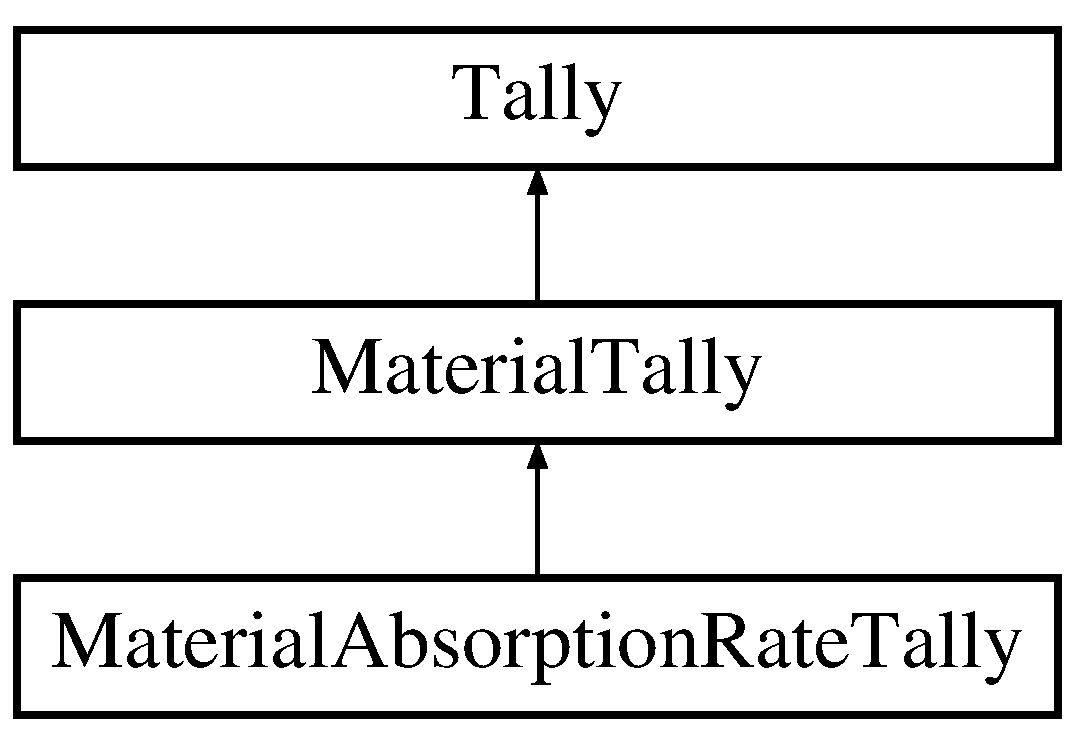
\includegraphics[height=3.000000cm]{classMaterialAbsorptionRateTally}
\end{center}
\end{figure}
\subsection*{Public Member Functions}
\begin{DoxyCompactItemize}
\item 
\hyperlink{classMaterialAbsorptionRateTally_a7623b08604df21dc42cd3da035d9bba6}{Material\-Absorption\-Rate\-Tally} (\hyperlink{classMaterial}{Material} $\ast$material, const char $\ast$tally\-\_\-name=(char $\ast$)\char`\"{}\char`\"{})
\begin{DoxyCompactList}\small\item\em \hyperlink{classMaterialAbsorptionRateTally}{Material\-Absorption\-Rate\-Tally} constructor calls the \hyperlink{classMaterialTally}{Material\-Tally} constructor and \hyperlink{classTally}{Tally} constructors and sets the tally type to A\-B\-S\-O\-R\-P\-T\-I\-O\-N\-\_\-\-R\-A\-T\-E. \end{DoxyCompactList}\item 
void \hyperlink{classMaterialAbsorptionRateTally_a86c4e2653f1baf2b862ce9d3043a888e}{tally} (\hyperlink{structneutron}{neutron} $\ast$\hyperlink{structneutron}{neutron})
\begin{DoxyCompactList}\small\item\em \hyperlink{classTally}{Tally} the material absorption rate by incrementing the tally by $ \frac{\Sigma_a}{\Sigma_t} $ at the neutron's energy. \end{DoxyCompactList}\end{DoxyCompactItemize}
\subsection*{Additional Inherited Members}


\subsection{Detailed Description}
A class for tallying the absorption rate within a material. 

\subsection{Constructor \& Destructor Documentation}
\hypertarget{classMaterialAbsorptionRateTally_a7623b08604df21dc42cd3da035d9bba6}{\index{Material\-Absorption\-Rate\-Tally@{Material\-Absorption\-Rate\-Tally}!Material\-Absorption\-Rate\-Tally@{Material\-Absorption\-Rate\-Tally}}
\index{Material\-Absorption\-Rate\-Tally@{Material\-Absorption\-Rate\-Tally}!MaterialAbsorptionRateTally@{Material\-Absorption\-Rate\-Tally}}
\subsubsection[{Material\-Absorption\-Rate\-Tally}]{\setlength{\rightskip}{0pt plus 5cm}Material\-Absorption\-Rate\-Tally\-::\-Material\-Absorption\-Rate\-Tally (
\begin{DoxyParamCaption}
\item[{{\bf Material} $\ast$}]{material, }
\item[{const char $\ast$}]{tally\-\_\-name = {\ttfamily (char$\ast$)\char`\"{}\char`\"{}}}
\end{DoxyParamCaption}
)\hspace{0.3cm}{\ttfamily [inline]}}}\label{classMaterialAbsorptionRateTally_a7623b08604df21dc42cd3da035d9bba6}


\hyperlink{classMaterialAbsorptionRateTally}{Material\-Absorption\-Rate\-Tally} constructor calls the \hyperlink{classMaterialTally}{Material\-Tally} constructor and \hyperlink{classTally}{Tally} constructors and sets the tally type to A\-B\-S\-O\-R\-P\-T\-I\-O\-N\-\_\-\-R\-A\-T\-E. 


\begin{DoxyParams}{Parameters}
{\em material} & a pointer to the material within which to tally \\
\hline
{\em tally\-\_\-name} & a character array for the tally name (optional) \\
\hline
\end{DoxyParams}


\subsection{Member Function Documentation}
\hypertarget{classMaterialAbsorptionRateTally_a86c4e2653f1baf2b862ce9d3043a888e}{\index{Material\-Absorption\-Rate\-Tally@{Material\-Absorption\-Rate\-Tally}!tally@{tally}}
\index{tally@{tally}!MaterialAbsorptionRateTally@{Material\-Absorption\-Rate\-Tally}}
\subsubsection[{tally}]{\setlength{\rightskip}{0pt plus 5cm}void Material\-Absorption\-Rate\-Tally\-::tally (
\begin{DoxyParamCaption}
\item[{{\bf neutron} $\ast$}]{neutron}
\end{DoxyParamCaption}
)\hspace{0.3cm}{\ttfamily [virtual]}}}\label{classMaterialAbsorptionRateTally_a86c4e2653f1baf2b862ce9d3043a888e}


\hyperlink{classTally}{Tally} the material absorption rate by incrementing the tally by $ \frac{\Sigma_a}{\Sigma_t} $ at the neutron's energy. 


\begin{DoxyParams}{Parameters}
{\em neutron} & the neutron of interest \\
\hline
\end{DoxyParams}


Implements \hyperlink{classMaterialTally_ab2debba62f51212ec8b39b7aeea3f54d}{Material\-Tally}.



The documentation for this class was generated from the following files\-:\begin{DoxyCompactItemize}
\item 
pinspec/src/\hyperlink{Tally_8h}{Tally.\-h}\item 
pinspec/src/Tally.\-cpp\end{DoxyCompactItemize}

\hypertarget{classMaterialCaptureRateTally}{\section{Material\-Capture\-Rate\-Tally Class Reference}
\label{classMaterialCaptureRateTally}\index{Material\-Capture\-Rate\-Tally@{Material\-Capture\-Rate\-Tally}}
}


A class for tallying the collision rate within a material.  




{\ttfamily \#include \char`\"{}pinspec/src/\-Tally.\-h\char`\"{}}

Inheritance diagram for Material\-Capture\-Rate\-Tally\-:\begin{figure}[H]
\begin{center}
\leavevmode
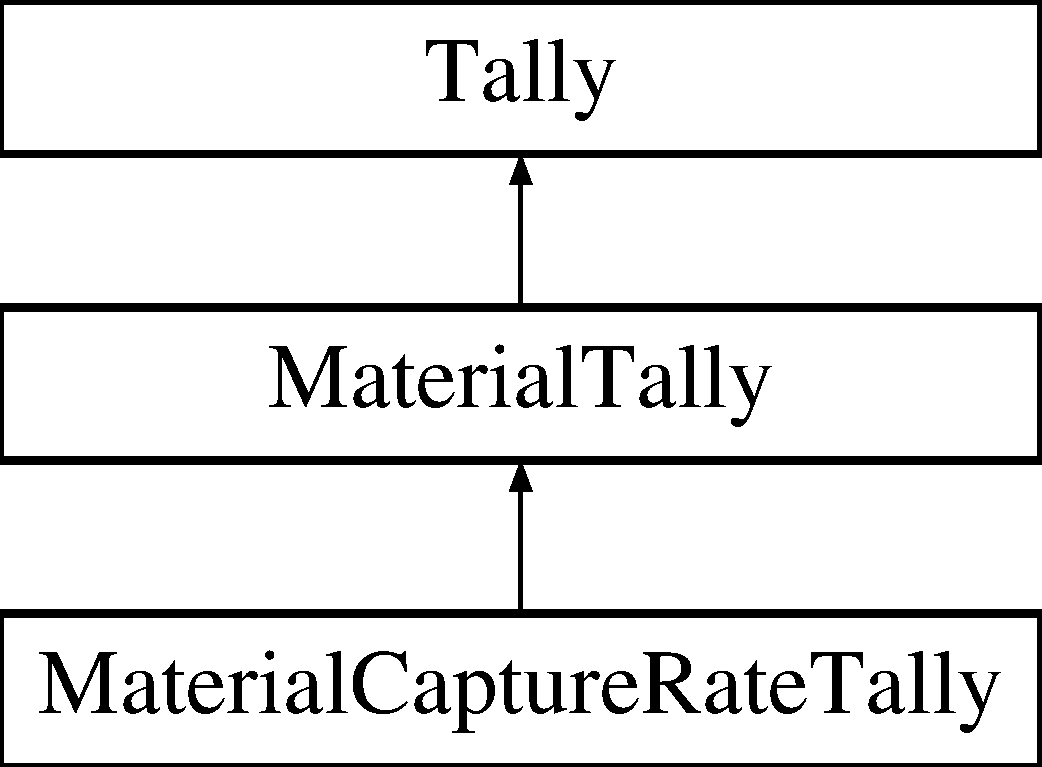
\includegraphics[height=3.000000cm]{classMaterialCaptureRateTally}
\end{center}
\end{figure}
\subsection*{Public Member Functions}
\begin{DoxyCompactItemize}
\item 
\hyperlink{classMaterialCaptureRateTally_ae2bad9a005cc081903041dd4675a2823}{Material\-Capture\-Rate\-Tally} (\hyperlink{classMaterial}{Material} $\ast$material, const char $\ast$tally\-\_\-name=(char $\ast$)\char`\"{}\char`\"{})
\begin{DoxyCompactList}\small\item\em \hyperlink{classMaterialCaptureRateTally}{Material\-Capture\-Rate\-Tally} constructor calls the \hyperlink{classIsotopeTally}{Isotope\-Tally} constructor and \hyperlink{classTally}{Tally} constructors and sets the tally type to C\-A\-P\-T\-U\-R\-E\-\_\-\-R\-A\-T\-E. \end{DoxyCompactList}\item 
void \hyperlink{classMaterialCaptureRateTally_a786889f9b19e47868b05b065920283e6}{tally} (\hyperlink{structneutron}{neutron} $\ast$\hyperlink{structneutron}{neutron})
\begin{DoxyCompactList}\small\item\em \hyperlink{classTally}{Tally} the material capture rate by incrementing the tally by $ \frac{\Sigma_c}{\Sigma_t} $ at the neutron's energy. \end{DoxyCompactList}\end{DoxyCompactItemize}
\subsection*{Additional Inherited Members}


\subsection{Detailed Description}
A class for tallying the collision rate within a material. 

\subsection{Constructor \& Destructor Documentation}
\hypertarget{classMaterialCaptureRateTally_ae2bad9a005cc081903041dd4675a2823}{\index{Material\-Capture\-Rate\-Tally@{Material\-Capture\-Rate\-Tally}!Material\-Capture\-Rate\-Tally@{Material\-Capture\-Rate\-Tally}}
\index{Material\-Capture\-Rate\-Tally@{Material\-Capture\-Rate\-Tally}!MaterialCaptureRateTally@{Material\-Capture\-Rate\-Tally}}
\subsubsection[{Material\-Capture\-Rate\-Tally}]{\setlength{\rightskip}{0pt plus 5cm}Material\-Capture\-Rate\-Tally\-::\-Material\-Capture\-Rate\-Tally (
\begin{DoxyParamCaption}
\item[{{\bf Material} $\ast$}]{material, }
\item[{const char $\ast$}]{tally\-\_\-name = {\ttfamily (char$\ast$)\char`\"{}\char`\"{}}}
\end{DoxyParamCaption}
)\hspace{0.3cm}{\ttfamily [inline]}}}\label{classMaterialCaptureRateTally_ae2bad9a005cc081903041dd4675a2823}


\hyperlink{classMaterialCaptureRateTally}{Material\-Capture\-Rate\-Tally} constructor calls the \hyperlink{classIsotopeTally}{Isotope\-Tally} constructor and \hyperlink{classTally}{Tally} constructors and sets the tally type to C\-A\-P\-T\-U\-R\-E\-\_\-\-R\-A\-T\-E. 


\begin{DoxyParams}{Parameters}
{\em material} & a pointer to the material within which to tally \\
\hline
{\em tally\-\_\-name} & a character array for the tally name (optional) \\
\hline
\end{DoxyParams}


\subsection{Member Function Documentation}
\hypertarget{classMaterialCaptureRateTally_a786889f9b19e47868b05b065920283e6}{\index{Material\-Capture\-Rate\-Tally@{Material\-Capture\-Rate\-Tally}!tally@{tally}}
\index{tally@{tally}!MaterialCaptureRateTally@{Material\-Capture\-Rate\-Tally}}
\subsubsection[{tally}]{\setlength{\rightskip}{0pt plus 5cm}void Material\-Capture\-Rate\-Tally\-::tally (
\begin{DoxyParamCaption}
\item[{{\bf neutron} $\ast$}]{neutron}
\end{DoxyParamCaption}
)\hspace{0.3cm}{\ttfamily [virtual]}}}\label{classMaterialCaptureRateTally_a786889f9b19e47868b05b065920283e6}


\hyperlink{classTally}{Tally} the material capture rate by incrementing the tally by $ \frac{\Sigma_c}{\Sigma_t} $ at the neutron's energy. 


\begin{DoxyParams}{Parameters}
{\em neutron} & the neutron of interest \\
\hline
\end{DoxyParams}


Implements \hyperlink{classMaterialTally_ab2debba62f51212ec8b39b7aeea3f54d}{Material\-Tally}.



The documentation for this class was generated from the following files\-:\begin{DoxyCompactItemize}
\item 
pinspec/src/\hyperlink{Tally_8h}{Tally.\-h}\item 
pinspec/src/Tally.\-cpp\end{DoxyCompactItemize}

\hypertarget{classMaterialCollisionRateTally}{\section{Material\-Collision\-Rate\-Tally Class Reference}
\label{classMaterialCollisionRateTally}\index{Material\-Collision\-Rate\-Tally@{Material\-Collision\-Rate\-Tally}}
}


A class for tallying the collision rate within a material.  




{\ttfamily \#include \char`\"{}pinspec/src/\-Tally.\-h\char`\"{}}

Inheritance diagram for Material\-Collision\-Rate\-Tally\-:\begin{figure}[H]
\begin{center}
\leavevmode
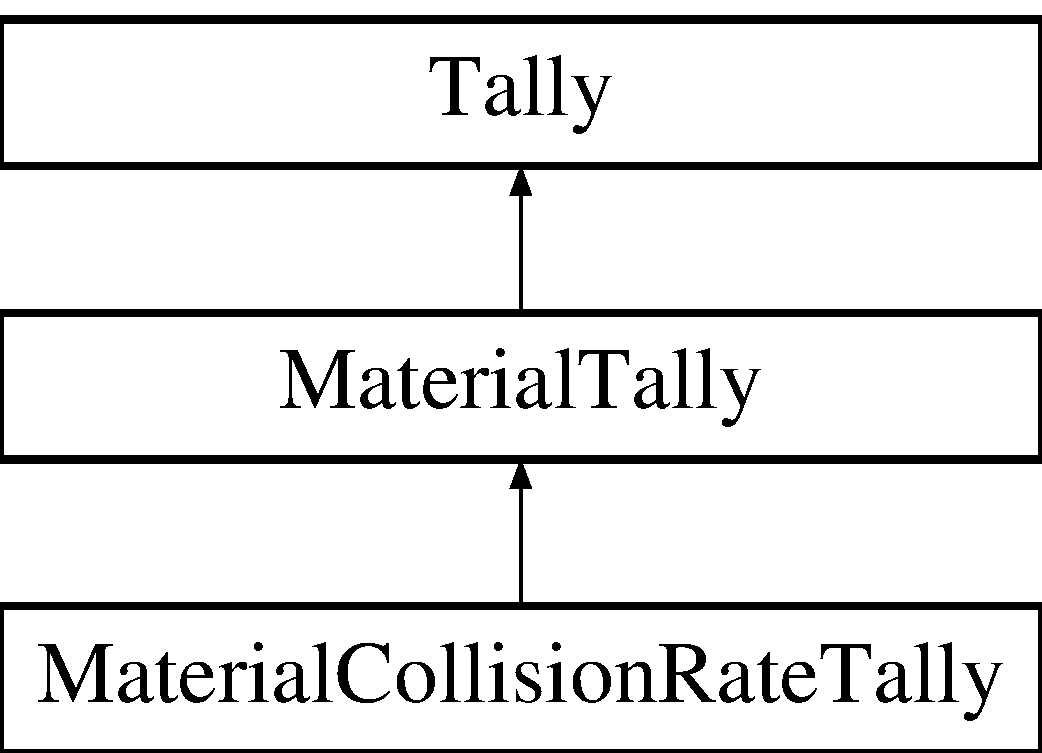
\includegraphics[height=3.000000cm]{classMaterialCollisionRateTally}
\end{center}
\end{figure}
\subsection*{Public Member Functions}
\begin{DoxyCompactItemize}
\item 
\hyperlink{classMaterialCollisionRateTally_a7513b0942fa1eab1a316c0f6dd5e7fdf}{Material\-Collision\-Rate\-Tally} (\hyperlink{classMaterial}{Material} $\ast$material, const char $\ast$tally\-\_\-name=(char $\ast$)\char`\"{}\char`\"{})
\begin{DoxyCompactList}\small\item\em \hyperlink{classMaterialCollisionRateTally}{Material\-Collision\-Rate\-Tally} constructor calls the \hyperlink{classMaterialTally}{Material\-Tally} constructor and \hyperlink{classTally}{Tally} constructors and sets the tally type to C\-O\-L\-L\-I\-S\-I\-O\-N\-\_\-\-R\-A\-T\-E. \end{DoxyCompactList}\item 
void \hyperlink{classMaterialCollisionRateTally_a3da8ad061bf2b1501a4f6a191ad5dfd9}{tally} (\hyperlink{structneutron}{neutron} $\ast$\hyperlink{structneutron}{neutron})
\begin{DoxyCompactList}\small\item\em \hyperlink{classTally}{Tally} the material collision rate by incrementing the tally by 1.\-0 at the neutron's energy. \end{DoxyCompactList}\end{DoxyCompactItemize}
\subsection*{Additional Inherited Members}


\subsection{Detailed Description}
A class for tallying the collision rate within a material. 

\subsection{Constructor \& Destructor Documentation}
\hypertarget{classMaterialCollisionRateTally_a7513b0942fa1eab1a316c0f6dd5e7fdf}{\index{Material\-Collision\-Rate\-Tally@{Material\-Collision\-Rate\-Tally}!Material\-Collision\-Rate\-Tally@{Material\-Collision\-Rate\-Tally}}
\index{Material\-Collision\-Rate\-Tally@{Material\-Collision\-Rate\-Tally}!MaterialCollisionRateTally@{Material\-Collision\-Rate\-Tally}}
\subsubsection[{Material\-Collision\-Rate\-Tally}]{\setlength{\rightskip}{0pt plus 5cm}Material\-Collision\-Rate\-Tally\-::\-Material\-Collision\-Rate\-Tally (
\begin{DoxyParamCaption}
\item[{{\bf Material} $\ast$}]{material, }
\item[{const char $\ast$}]{tally\-\_\-name = {\ttfamily (char$\ast$)\char`\"{}\char`\"{}}}
\end{DoxyParamCaption}
)\hspace{0.3cm}{\ttfamily [inline]}}}\label{classMaterialCollisionRateTally_a7513b0942fa1eab1a316c0f6dd5e7fdf}


\hyperlink{classMaterialCollisionRateTally}{Material\-Collision\-Rate\-Tally} constructor calls the \hyperlink{classMaterialTally}{Material\-Tally} constructor and \hyperlink{classTally}{Tally} constructors and sets the tally type to C\-O\-L\-L\-I\-S\-I\-O\-N\-\_\-\-R\-A\-T\-E. 


\begin{DoxyParams}{Parameters}
{\em material} & a pointer to the material within which to tally \\
\hline
{\em tally\-\_\-name} & a character array for the tally name (optional) \\
\hline
\end{DoxyParams}


\subsection{Member Function Documentation}
\hypertarget{classMaterialCollisionRateTally_a3da8ad061bf2b1501a4f6a191ad5dfd9}{\index{Material\-Collision\-Rate\-Tally@{Material\-Collision\-Rate\-Tally}!tally@{tally}}
\index{tally@{tally}!MaterialCollisionRateTally@{Material\-Collision\-Rate\-Tally}}
\subsubsection[{tally}]{\setlength{\rightskip}{0pt plus 5cm}void Material\-Collision\-Rate\-Tally\-::tally (
\begin{DoxyParamCaption}
\item[{{\bf neutron} $\ast$}]{neutron}
\end{DoxyParamCaption}
)\hspace{0.3cm}{\ttfamily [virtual]}}}\label{classMaterialCollisionRateTally_a3da8ad061bf2b1501a4f6a191ad5dfd9}


\hyperlink{classTally}{Tally} the material collision rate by incrementing the tally by 1.\-0 at the neutron's energy. 


\begin{DoxyParams}{Parameters}
{\em neutron} & the neutron of interest \\
\hline
\end{DoxyParams}


Implements \hyperlink{classMaterialTally_ab2debba62f51212ec8b39b7aeea3f54d}{Material\-Tally}.



The documentation for this class was generated from the following files\-:\begin{DoxyCompactItemize}
\item 
pinspec/src/\hyperlink{Tally_8h}{Tally.\-h}\item 
pinspec/src/Tally.\-cpp\end{DoxyCompactItemize}

\hypertarget{classMaterialDiffusionRateTally}{\section{Material\-Diffusion\-Rate\-Tally Class Reference}
\label{classMaterialDiffusionRateTally}\index{Material\-Diffusion\-Rate\-Tally@{Material\-Diffusion\-Rate\-Tally}}
}


A class for tallying the diffusion rate within a material.  




{\ttfamily \#include \char`\"{}pinspec/src/\-Tally.\-h\char`\"{}}

Inheritance diagram for Material\-Diffusion\-Rate\-Tally\-:\begin{figure}[H]
\begin{center}
\leavevmode
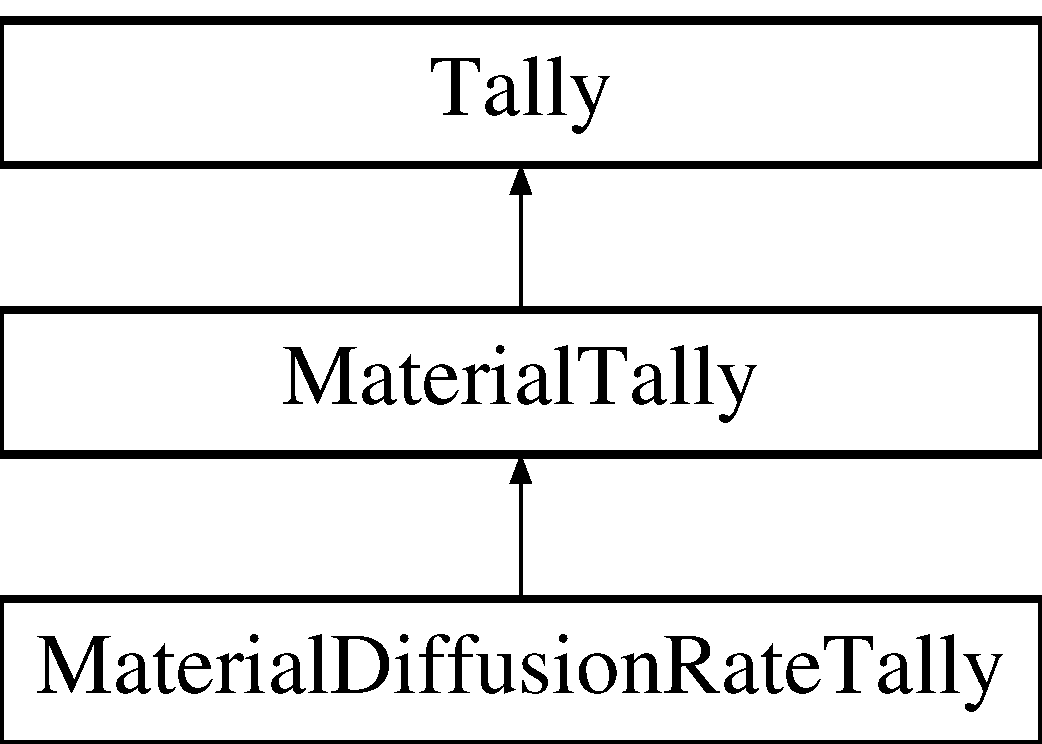
\includegraphics[height=3.000000cm]{classMaterialDiffusionRateTally}
\end{center}
\end{figure}
\subsection*{Public Member Functions}
\begin{DoxyCompactItemize}
\item 
\hyperlink{classMaterialDiffusionRateTally_a5339ada27f620235e11547d008d91f95}{Material\-Diffusion\-Rate\-Tally} (\hyperlink{classMaterial}{Material} $\ast$material, const char $\ast$tally\-\_\-name=(char $\ast$)\char`\"{}\char`\"{})
\begin{DoxyCompactList}\small\item\em \hyperlink{classMaterialDiffusionRateTally}{Material\-Diffusion\-Rate\-Tally} constructor calls the \hyperlink{classMaterialTally}{Material\-Tally} constructor and \hyperlink{classTally}{Tally} constructors and sets the tally type to D\-I\-F\-F\-U\-S\-I\-O\-N\-\_\-\-R\-A\-T\-E. \end{DoxyCompactList}\item 
void \hyperlink{classMaterialDiffusionRateTally_a63bd04bab0e138059384e35d925a5ce0}{tally} (\hyperlink{structneutron}{neutron} $\ast$\hyperlink{structneutron}{neutron})
\begin{DoxyCompactList}\small\item\em \hyperlink{classTally}{Tally} the material diffusion rate by incrementing the tally by $ \frac{\frac{1}{3\Sigma_tr}}{\Sigma_t} $ at the neutron's energy. \end{DoxyCompactList}\end{DoxyCompactItemize}
\subsection*{Additional Inherited Members}


\subsection{Detailed Description}
A class for tallying the diffusion rate within a material. 

\subsection{Constructor \& Destructor Documentation}
\hypertarget{classMaterialDiffusionRateTally_a5339ada27f620235e11547d008d91f95}{\index{Material\-Diffusion\-Rate\-Tally@{Material\-Diffusion\-Rate\-Tally}!Material\-Diffusion\-Rate\-Tally@{Material\-Diffusion\-Rate\-Tally}}
\index{Material\-Diffusion\-Rate\-Tally@{Material\-Diffusion\-Rate\-Tally}!MaterialDiffusionRateTally@{Material\-Diffusion\-Rate\-Tally}}
\subsubsection[{Material\-Diffusion\-Rate\-Tally}]{\setlength{\rightskip}{0pt plus 5cm}Material\-Diffusion\-Rate\-Tally\-::\-Material\-Diffusion\-Rate\-Tally (
\begin{DoxyParamCaption}
\item[{{\bf Material} $\ast$}]{material, }
\item[{const char $\ast$}]{tally\-\_\-name = {\ttfamily (char$\ast$)\char`\"{}\char`\"{}}}
\end{DoxyParamCaption}
)\hspace{0.3cm}{\ttfamily [inline]}}}\label{classMaterialDiffusionRateTally_a5339ada27f620235e11547d008d91f95}


\hyperlink{classMaterialDiffusionRateTally}{Material\-Diffusion\-Rate\-Tally} constructor calls the \hyperlink{classMaterialTally}{Material\-Tally} constructor and \hyperlink{classTally}{Tally} constructors and sets the tally type to D\-I\-F\-F\-U\-S\-I\-O\-N\-\_\-\-R\-A\-T\-E. 


\begin{DoxyParams}{Parameters}
{\em material} & a pointer to the material within which to tally \\
\hline
{\em tally\-\_\-name} & a character array for the tally name (optional) \\
\hline
\end{DoxyParams}


\subsection{Member Function Documentation}
\hypertarget{classMaterialDiffusionRateTally_a63bd04bab0e138059384e35d925a5ce0}{\index{Material\-Diffusion\-Rate\-Tally@{Material\-Diffusion\-Rate\-Tally}!tally@{tally}}
\index{tally@{tally}!MaterialDiffusionRateTally@{Material\-Diffusion\-Rate\-Tally}}
\subsubsection[{tally}]{\setlength{\rightskip}{0pt plus 5cm}void Material\-Diffusion\-Rate\-Tally\-::tally (
\begin{DoxyParamCaption}
\item[{{\bf neutron} $\ast$}]{neutron}
\end{DoxyParamCaption}
)\hspace{0.3cm}{\ttfamily [virtual]}}}\label{classMaterialDiffusionRateTally_a63bd04bab0e138059384e35d925a5ce0}


\hyperlink{classTally}{Tally} the material diffusion rate by incrementing the tally by $ \frac{\frac{1}{3\Sigma_tr}}{\Sigma_t} $ at the neutron's energy. 


\begin{DoxyParams}{Parameters}
{\em neutron} & the neutron of interest \\
\hline
\end{DoxyParams}


Implements \hyperlink{classMaterialTally_ab2debba62f51212ec8b39b7aeea3f54d}{Material\-Tally}.



The documentation for this class was generated from the following files\-:\begin{DoxyCompactItemize}
\item 
\hyperlink{Tally_8h}{Tally.\-h}\item 
Tally.\-cpp\end{DoxyCompactItemize}

\hypertarget{classMaterialElasticRateTally}{\section{Material\-Elastic\-Rate\-Tally Class Reference}
\label{classMaterialElasticRateTally}\index{Material\-Elastic\-Rate\-Tally@{Material\-Elastic\-Rate\-Tally}}
}


A class for tallying the elastic scattering rate within a material.  




{\ttfamily \#include \char`\"{}pinspec/src/\-Tally.\-h\char`\"{}}

Inheritance diagram for Material\-Elastic\-Rate\-Tally\-:\begin{figure}[H]
\begin{center}
\leavevmode
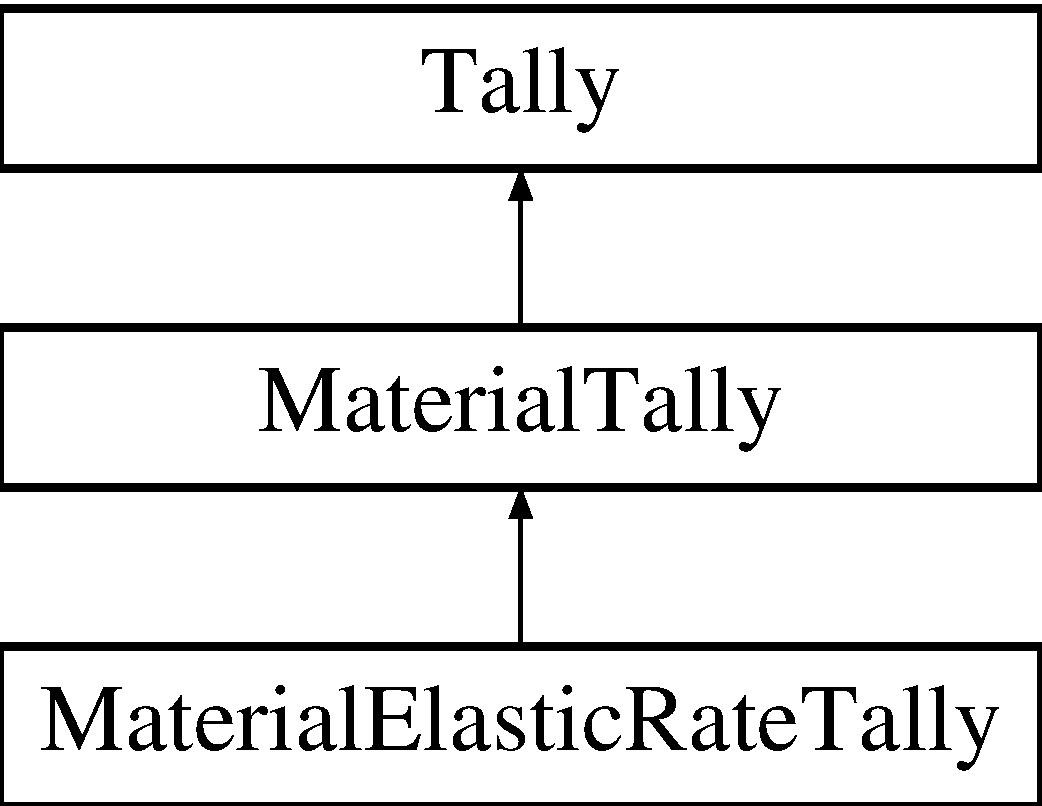
\includegraphics[height=3.000000cm]{classMaterialElasticRateTally}
\end{center}
\end{figure}
\subsection*{Public Member Functions}
\begin{DoxyCompactItemize}
\item 
\hyperlink{classMaterialElasticRateTally_a4f2365c949a7bc093c4c71484363daa3}{Material\-Elastic\-Rate\-Tally} (\hyperlink{classMaterial}{Material} $\ast$material, const char $\ast$tally\-\_\-name=(char $\ast$)\char`\"{}\char`\"{})
\begin{DoxyCompactList}\small\item\em \hyperlink{classMaterialCollisionRateTally}{Material\-Collision\-Rate\-Tally} constructor calls the \hyperlink{classMaterialTally}{Material\-Tally} constructor and \hyperlink{classTally}{Tally} constructors and sets the tally type to E\-L\-A\-S\-T\-I\-C\-\_\-\-R\-A\-T\-E. \end{DoxyCompactList}\item 
void \hyperlink{classMaterialElasticRateTally_a8d3104a906c10b34c236275f65aa610d}{tally} (\hyperlink{structneutron}{neutron} $\ast$\hyperlink{structneutron}{neutron})
\begin{DoxyCompactList}\small\item\em \hyperlink{classTally}{Tally} the material elastic scattering rate by incrementing the tally by $ \frac{\Sigma_s}{\Sigma_t} $ at the neutron's energy. \end{DoxyCompactList}\end{DoxyCompactItemize}
\subsection*{Additional Inherited Members}


\subsection{Detailed Description}
A class for tallying the elastic scattering rate within a material. 

\subsection{Constructor \& Destructor Documentation}
\hypertarget{classMaterialElasticRateTally_a4f2365c949a7bc093c4c71484363daa3}{\index{Material\-Elastic\-Rate\-Tally@{Material\-Elastic\-Rate\-Tally}!Material\-Elastic\-Rate\-Tally@{Material\-Elastic\-Rate\-Tally}}
\index{Material\-Elastic\-Rate\-Tally@{Material\-Elastic\-Rate\-Tally}!MaterialElasticRateTally@{Material\-Elastic\-Rate\-Tally}}
\subsubsection[{Material\-Elastic\-Rate\-Tally}]{\setlength{\rightskip}{0pt plus 5cm}Material\-Elastic\-Rate\-Tally\-::\-Material\-Elastic\-Rate\-Tally (
\begin{DoxyParamCaption}
\item[{{\bf Material} $\ast$}]{material, }
\item[{const char $\ast$}]{tally\-\_\-name = {\ttfamily (char$\ast$)\char`\"{}\char`\"{}}}
\end{DoxyParamCaption}
)\hspace{0.3cm}{\ttfamily [inline]}}}\label{classMaterialElasticRateTally_a4f2365c949a7bc093c4c71484363daa3}


\hyperlink{classMaterialCollisionRateTally}{Material\-Collision\-Rate\-Tally} constructor calls the \hyperlink{classMaterialTally}{Material\-Tally} constructor and \hyperlink{classTally}{Tally} constructors and sets the tally type to E\-L\-A\-S\-T\-I\-C\-\_\-\-R\-A\-T\-E. 


\begin{DoxyParams}{Parameters}
{\em material} & a pointer to the material within which to tally \\
\hline
{\em tally\-\_\-name} & a character array for the tally name (optional) \\
\hline
\end{DoxyParams}


\subsection{Member Function Documentation}
\hypertarget{classMaterialElasticRateTally_a8d3104a906c10b34c236275f65aa610d}{\index{Material\-Elastic\-Rate\-Tally@{Material\-Elastic\-Rate\-Tally}!tally@{tally}}
\index{tally@{tally}!MaterialElasticRateTally@{Material\-Elastic\-Rate\-Tally}}
\subsubsection[{tally}]{\setlength{\rightskip}{0pt plus 5cm}void Material\-Elastic\-Rate\-Tally\-::tally (
\begin{DoxyParamCaption}
\item[{{\bf neutron} $\ast$}]{neutron}
\end{DoxyParamCaption}
)\hspace{0.3cm}{\ttfamily [virtual]}}}\label{classMaterialElasticRateTally_a8d3104a906c10b34c236275f65aa610d}


\hyperlink{classTally}{Tally} the material elastic scattering rate by incrementing the tally by $ \frac{\Sigma_s}{\Sigma_t} $ at the neutron's energy. 


\begin{DoxyParams}{Parameters}
{\em neutron} & the neutron of interest \\
\hline
\end{DoxyParams}


Implements \hyperlink{classMaterialTally_ab2debba62f51212ec8b39b7aeea3f54d}{Material\-Tally}.



The documentation for this class was generated from the following files\-:\begin{DoxyCompactItemize}
\item 
\hyperlink{Tally_8h}{Tally.\-h}\item 
Tally.\-cpp\end{DoxyCompactItemize}

\hypertarget{classMaterialFissionRateTally}{\section{Material\-Fission\-Rate\-Tally Class Reference}
\label{classMaterialFissionRateTally}\index{Material\-Fission\-Rate\-Tally@{Material\-Fission\-Rate\-Tally}}
}


A class for tallying the capture rate within a material.  




{\ttfamily \#include \char`\"{}pinspec/src/\-Tally.\-h\char`\"{}}

Inheritance diagram for Material\-Fission\-Rate\-Tally\-:\begin{figure}[H]
\begin{center}
\leavevmode
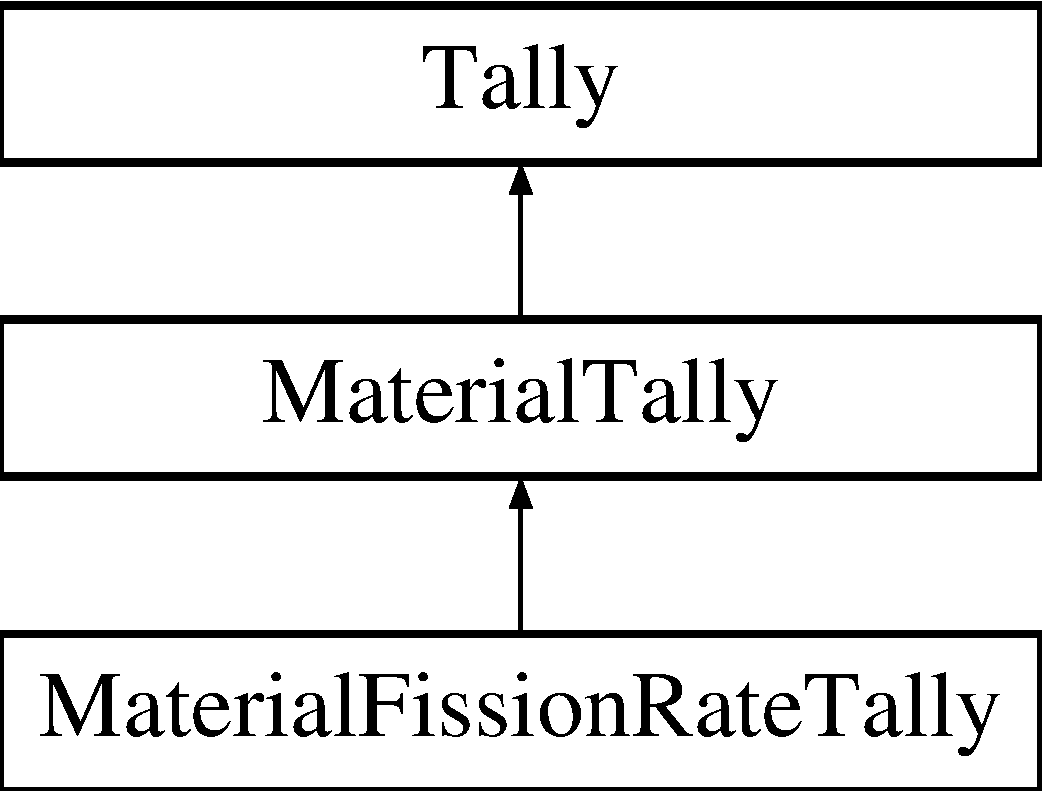
\includegraphics[height=3.000000cm]{classMaterialFissionRateTally}
\end{center}
\end{figure}
\subsection*{Public Member Functions}
\begin{DoxyCompactItemize}
\item 
\hyperlink{classMaterialFissionRateTally_a3ef088c0910245eab495e6921af55caa}{Material\-Fission\-Rate\-Tally} (\hyperlink{classMaterial}{Material} $\ast$material, const char $\ast$tally\-\_\-name=(char $\ast$)\char`\"{}\char`\"{})
\begin{DoxyCompactList}\small\item\em \hyperlink{classMaterialFissionRateTally}{Material\-Fission\-Rate\-Tally} constructor calls the \hyperlink{classMaterialTally}{Material\-Tally} constructor and \hyperlink{classTally}{Tally} constructors and sets the tally type to F\-I\-S\-S\-I\-O\-N\-\_\-\-R\-A\-T\-E. \end{DoxyCompactList}\item 
void \hyperlink{classMaterialFissionRateTally_aa47cb28d567ce9315872fff4251dce31}{tally} (\hyperlink{structneutron}{neutron} $\ast$\hyperlink{structneutron}{neutron})
\begin{DoxyCompactList}\small\item\em \hyperlink{classTally}{Tally} the material fission rate by incrementing the tally by $ \frac{\Sigma_f}{\Sigma_t} $ at the neutron's energy. \end{DoxyCompactList}\end{DoxyCompactItemize}
\subsection*{Additional Inherited Members}


\subsection{Detailed Description}
A class for tallying the capture rate within a material. 

\subsection{Constructor \& Destructor Documentation}
\hypertarget{classMaterialFissionRateTally_a3ef088c0910245eab495e6921af55caa}{\index{Material\-Fission\-Rate\-Tally@{Material\-Fission\-Rate\-Tally}!Material\-Fission\-Rate\-Tally@{Material\-Fission\-Rate\-Tally}}
\index{Material\-Fission\-Rate\-Tally@{Material\-Fission\-Rate\-Tally}!MaterialFissionRateTally@{Material\-Fission\-Rate\-Tally}}
\subsubsection[{Material\-Fission\-Rate\-Tally}]{\setlength{\rightskip}{0pt plus 5cm}Material\-Fission\-Rate\-Tally\-::\-Material\-Fission\-Rate\-Tally (
\begin{DoxyParamCaption}
\item[{{\bf Material} $\ast$}]{material, }
\item[{const char $\ast$}]{tally\-\_\-name = {\ttfamily (char$\ast$)\char`\"{}\char`\"{}}}
\end{DoxyParamCaption}
)\hspace{0.3cm}{\ttfamily [inline]}}}\label{classMaterialFissionRateTally_a3ef088c0910245eab495e6921af55caa}


\hyperlink{classMaterialFissionRateTally}{Material\-Fission\-Rate\-Tally} constructor calls the \hyperlink{classMaterialTally}{Material\-Tally} constructor and \hyperlink{classTally}{Tally} constructors and sets the tally type to F\-I\-S\-S\-I\-O\-N\-\_\-\-R\-A\-T\-E. 


\begin{DoxyParams}{Parameters}
{\em material} & a pointer to the material within which to tally \\
\hline
{\em tally\-\_\-name} & a character array for the tally name (optional) \\
\hline
\end{DoxyParams}


\subsection{Member Function Documentation}
\hypertarget{classMaterialFissionRateTally_aa47cb28d567ce9315872fff4251dce31}{\index{Material\-Fission\-Rate\-Tally@{Material\-Fission\-Rate\-Tally}!tally@{tally}}
\index{tally@{tally}!MaterialFissionRateTally@{Material\-Fission\-Rate\-Tally}}
\subsubsection[{tally}]{\setlength{\rightskip}{0pt plus 5cm}void Material\-Fission\-Rate\-Tally\-::tally (
\begin{DoxyParamCaption}
\item[{{\bf neutron} $\ast$}]{neutron}
\end{DoxyParamCaption}
)\hspace{0.3cm}{\ttfamily [virtual]}}}\label{classMaterialFissionRateTally_aa47cb28d567ce9315872fff4251dce31}


\hyperlink{classTally}{Tally} the material fission rate by incrementing the tally by $ \frac{\Sigma_f}{\Sigma_t} $ at the neutron's energy. 


\begin{DoxyParams}{Parameters}
{\em neutron} & the neutron of interest \\
\hline
\end{DoxyParams}


Implements \hyperlink{classMaterialTally_ab2debba62f51212ec8b39b7aeea3f54d}{Material\-Tally}.



The documentation for this class was generated from the following files\-:\begin{DoxyCompactItemize}
\item 
pinspec/src/\hyperlink{Tally_8h}{Tally.\-h}\item 
pinspec/src/Tally.\-cpp\end{DoxyCompactItemize}

\hypertarget{classMaterialFluxTally}{\section{Material\-Flux\-Tally Class Reference}
\label{classMaterialFluxTally}\index{Material\-Flux\-Tally@{Material\-Flux\-Tally}}
}


A class for tallying the flux in all regions filled by a material.  




{\ttfamily \#include \char`\"{}pinspec/src/\-Tally.\-h\char`\"{}}

Inheritance diagram for Material\-Flux\-Tally\-:\begin{figure}[H]
\begin{center}
\leavevmode
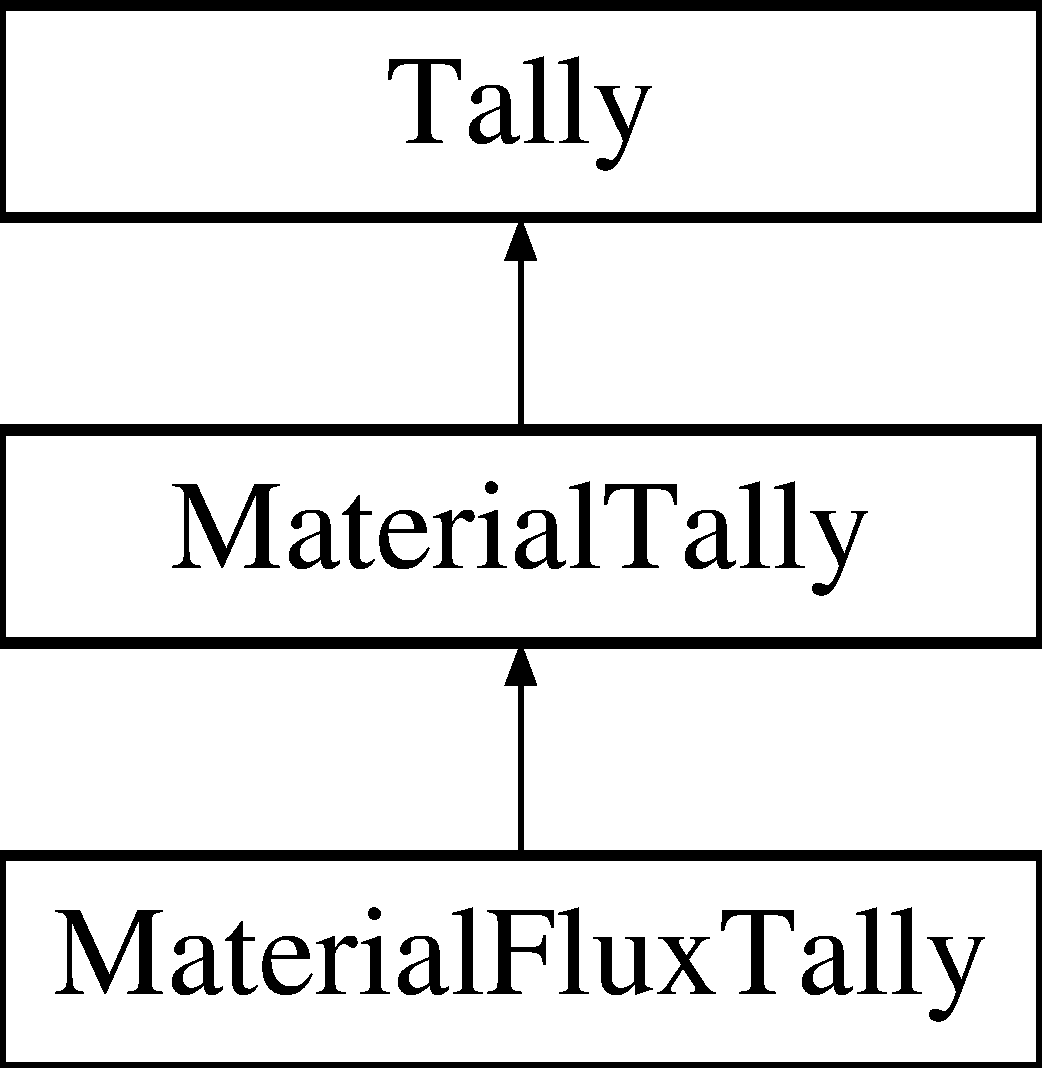
\includegraphics[height=3.000000cm]{classMaterialFluxTally}
\end{center}
\end{figure}
\subsection*{Public Member Functions}
\begin{DoxyCompactItemize}
\item 
\hyperlink{classMaterialFluxTally_ab1deeebac35f38d8f3c56f1b5c4b0eb5}{Material\-Flux\-Tally} (\hyperlink{classMaterial}{Material} $\ast$material, const char $\ast$tally\-\_\-name=(char $\ast$)\char`\"{}\char`\"{})
\begin{DoxyCompactList}\small\item\em \hyperlink{classIsotopeCaptureRateTally}{Isotope\-Capture\-Rate\-Tally} constructor calls the \hyperlink{classMaterialTally}{Material\-Tally} constructor and \hyperlink{classTally}{Tally} constructors and sets the tally type to F\-L\-U\-X. \end{DoxyCompactList}\item 
void \hyperlink{classMaterialFluxTally_a458d77b55dbd6bd0fb5efeb2ffec2e9b}{tally} (\hyperlink{structneutron}{neutron} $\ast$\hyperlink{structneutron}{neutron})
\begin{DoxyCompactList}\small\item\em \hyperlink{classTally}{Tally} the material flux by incrementing the tally by $ \frac{1}{\Sigma_t} $ at the neutron's energy. \end{DoxyCompactList}\end{DoxyCompactItemize}
\subsection*{Additional Inherited Members}


\subsection{Detailed Description}
A class for tallying the flux in all regions filled by a material. 

\subsection{Constructor \& Destructor Documentation}
\hypertarget{classMaterialFluxTally_ab1deeebac35f38d8f3c56f1b5c4b0eb5}{\index{Material\-Flux\-Tally@{Material\-Flux\-Tally}!Material\-Flux\-Tally@{Material\-Flux\-Tally}}
\index{Material\-Flux\-Tally@{Material\-Flux\-Tally}!MaterialFluxTally@{Material\-Flux\-Tally}}
\subsubsection[{Material\-Flux\-Tally}]{\setlength{\rightskip}{0pt plus 5cm}Material\-Flux\-Tally\-::\-Material\-Flux\-Tally (
\begin{DoxyParamCaption}
\item[{{\bf Material} $\ast$}]{material, }
\item[{const char $\ast$}]{tally\-\_\-name = {\ttfamily (char$\ast$)\char`\"{}\char`\"{}}}
\end{DoxyParamCaption}
)\hspace{0.3cm}{\ttfamily [inline]}}}\label{classMaterialFluxTally_ab1deeebac35f38d8f3c56f1b5c4b0eb5}


\hyperlink{classIsotopeCaptureRateTally}{Isotope\-Capture\-Rate\-Tally} constructor calls the \hyperlink{classMaterialTally}{Material\-Tally} constructor and \hyperlink{classTally}{Tally} constructors and sets the tally type to F\-L\-U\-X. 


\begin{DoxyParams}{Parameters}
{\em material} & a pointer to the material within which to tally \\
\hline
{\em tally\-\_\-name} & a character array for the tally name (optional) \\
\hline
\end{DoxyParams}


\subsection{Member Function Documentation}
\hypertarget{classMaterialFluxTally_a458d77b55dbd6bd0fb5efeb2ffec2e9b}{\index{Material\-Flux\-Tally@{Material\-Flux\-Tally}!tally@{tally}}
\index{tally@{tally}!MaterialFluxTally@{Material\-Flux\-Tally}}
\subsubsection[{tally}]{\setlength{\rightskip}{0pt plus 5cm}void Material\-Flux\-Tally\-::tally (
\begin{DoxyParamCaption}
\item[{{\bf neutron} $\ast$}]{neutron}
\end{DoxyParamCaption}
)\hspace{0.3cm}{\ttfamily [virtual]}}}\label{classMaterialFluxTally_a458d77b55dbd6bd0fb5efeb2ffec2e9b}


\hyperlink{classTally}{Tally} the material flux by incrementing the tally by $ \frac{1}{\Sigma_t} $ at the neutron's energy. 


\begin{DoxyParams}{Parameters}
{\em neutron} & the neutron of interest \\
\hline
\end{DoxyParams}


Implements \hyperlink{classMaterialTally_ab2debba62f51212ec8b39b7aeea3f54d}{Material\-Tally}.



The documentation for this class was generated from the following files\-:\begin{DoxyCompactItemize}
\item 
pinspec/src/\hyperlink{Tally_8h}{Tally.\-h}\item 
pinspec/src/Tally.\-cpp\end{DoxyCompactItemize}

\hypertarget{classMaterialInterCollisionTimeTally}{\section{Material\-Inter\-Collision\-Time\-Tally Class Reference}
\label{classMaterialInterCollisionTimeTally}\index{Material\-Inter\-Collision\-Time\-Tally@{Material\-Inter\-Collision\-Time\-Tally}}
}


A class for tallying the time between collision with a material.  




{\ttfamily \#include \char`\"{}pinspec/src/\-Tally.\-h\char`\"{}}

Inheritance diagram for Material\-Inter\-Collision\-Time\-Tally\-:\begin{figure}[H]
\begin{center}
\leavevmode
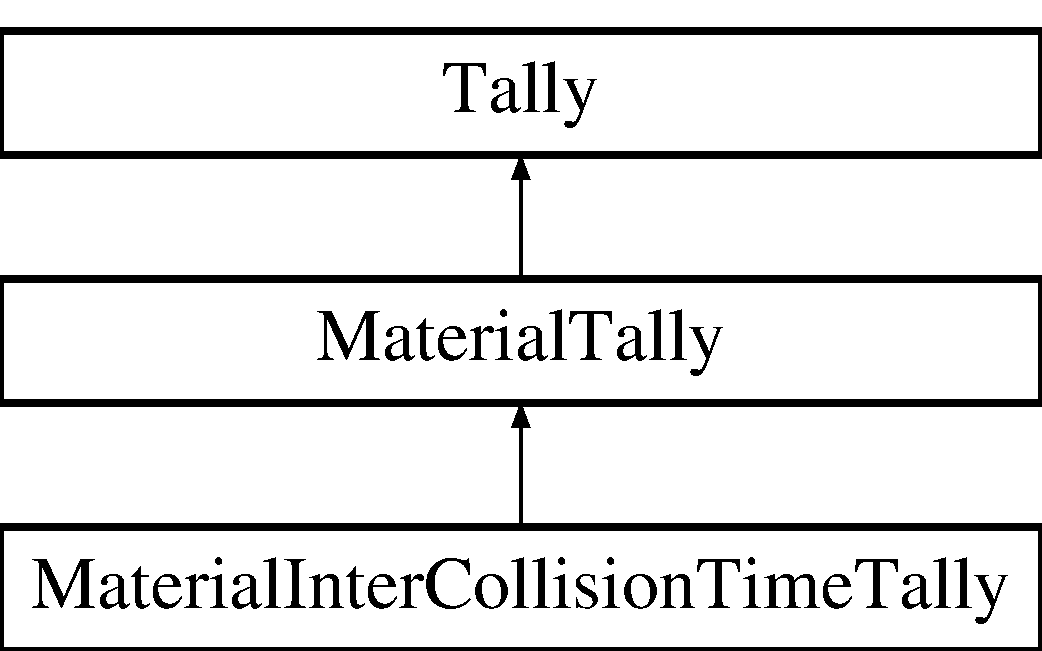
\includegraphics[height=3.000000cm]{classMaterialInterCollisionTimeTally}
\end{center}
\end{figure}
\subsection*{Public Member Functions}
\begin{DoxyCompactItemize}
\item 
\hyperlink{classMaterialInterCollisionTimeTally_a76049b7e29408581586c8f8ae1b50293}{Material\-Inter\-Collision\-Time\-Tally} (\hyperlink{classMaterial}{Material} $\ast$material, const char $\ast$tally\-\_\-name=(char $\ast$)\char`\"{}\char`\"{})
\begin{DoxyCompactList}\small\item\em \hyperlink{classMaterialInterCollisionTimeTally}{Material\-Inter\-Collision\-Time\-Tally} constructor calls the \hyperlink{classMaterialTally}{Material\-Tally} constructor and \hyperlink{classTally}{Tally} constructors and sets the tally type to I\-N\-T\-E\-R\-C\-O\-L\-L\-I\-S\-I\-O\-N\-\_\-\-T\-I\-M\-E. \end{DoxyCompactList}\item 
void \hyperlink{classMaterialInterCollisionTimeTally_a339ebb3a0367954d650006acc72185b9}{tally} (\hyperlink{structneutron}{neutron} $\ast$\hyperlink{structneutron}{neutron})
\begin{DoxyCompactList}\small\item\em \hyperlink{classTally}{Tally} the time between collisions by incrementing the tally with the travel time spent by this neutron to reach this collision\-: \end{DoxyCompactList}\end{DoxyCompactItemize}
\subsection*{Additional Inherited Members}


\subsection{Detailed Description}
A class for tallying the time between collision with a material. 

\subsection{Constructor \& Destructor Documentation}
\hypertarget{classMaterialInterCollisionTimeTally_a76049b7e29408581586c8f8ae1b50293}{\index{Material\-Inter\-Collision\-Time\-Tally@{Material\-Inter\-Collision\-Time\-Tally}!Material\-Inter\-Collision\-Time\-Tally@{Material\-Inter\-Collision\-Time\-Tally}}
\index{Material\-Inter\-Collision\-Time\-Tally@{Material\-Inter\-Collision\-Time\-Tally}!MaterialInterCollisionTimeTally@{Material\-Inter\-Collision\-Time\-Tally}}
\subsubsection[{Material\-Inter\-Collision\-Time\-Tally}]{\setlength{\rightskip}{0pt plus 5cm}Material\-Inter\-Collision\-Time\-Tally\-::\-Material\-Inter\-Collision\-Time\-Tally (
\begin{DoxyParamCaption}
\item[{{\bf Material} $\ast$}]{material, }
\item[{const char $\ast$}]{tally\-\_\-name = {\ttfamily (char$\ast$)\char`\"{}\char`\"{}}}
\end{DoxyParamCaption}
)\hspace{0.3cm}{\ttfamily [inline]}}}\label{classMaterialInterCollisionTimeTally_a76049b7e29408581586c8f8ae1b50293}


\hyperlink{classMaterialInterCollisionTimeTally}{Material\-Inter\-Collision\-Time\-Tally} constructor calls the \hyperlink{classMaterialTally}{Material\-Tally} constructor and \hyperlink{classTally}{Tally} constructors and sets the tally type to I\-N\-T\-E\-R\-C\-O\-L\-L\-I\-S\-I\-O\-N\-\_\-\-T\-I\-M\-E. 


\begin{DoxyParams}{Parameters}
{\em material} & a pointer to the material within which to tally \\
\hline
{\em tally\-\_\-name} & a character array for the tally name (optional) \\
\hline
\end{DoxyParams}


\subsection{Member Function Documentation}
\hypertarget{classMaterialInterCollisionTimeTally_a339ebb3a0367954d650006acc72185b9}{\index{Material\-Inter\-Collision\-Time\-Tally@{Material\-Inter\-Collision\-Time\-Tally}!tally@{tally}}
\index{tally@{tally}!MaterialInterCollisionTimeTally@{Material\-Inter\-Collision\-Time\-Tally}}
\subsubsection[{tally}]{\setlength{\rightskip}{0pt plus 5cm}void Material\-Inter\-Collision\-Time\-Tally\-::tally (
\begin{DoxyParamCaption}
\item[{{\bf neutron} $\ast$}]{neutron}
\end{DoxyParamCaption}
)\hspace{0.3cm}{\ttfamily [virtual]}}}\label{classMaterialInterCollisionTimeTally_a339ebb3a0367954d650006acc72185b9}


\hyperlink{classTally}{Tally} the time between collisions by incrementing the tally with the travel time spent by this neutron to reach this collision\-: 

$ d = \frac{1}{\Sigma_t} $ $ v = c\sqrt{2Em_n} $ $ time = \frac{d}{v} $ 
\begin{DoxyParams}{Parameters}
{\em neutron} & the neutron of interest \\
\hline
\end{DoxyParams}


Implements \hyperlink{classMaterialTally_ab2debba62f51212ec8b39b7aeea3f54d}{Material\-Tally}.



The documentation for this class was generated from the following files\-:\begin{DoxyCompactItemize}
\item 
pinspec/src/\hyperlink{Tally_8h}{Tally.\-h}\item 
pinspec/src/Tally.\-cpp\end{DoxyCompactItemize}

\hypertarget{classMaterialLeakageRateTally}{\section{Material\-Leakage\-Rate\-Tally Class Reference}
\label{classMaterialLeakageRateTally}\index{Material\-Leakage\-Rate\-Tally@{Material\-Leakage\-Rate\-Tally}}
}


A class for tallying the leakage rate for the regions filled by a material.  




{\ttfamily \#include \char`\"{}pinspec/src/\-Tally.\-h\char`\"{}}

Inheritance diagram for Material\-Leakage\-Rate\-Tally\-:\begin{figure}[H]
\begin{center}
\leavevmode
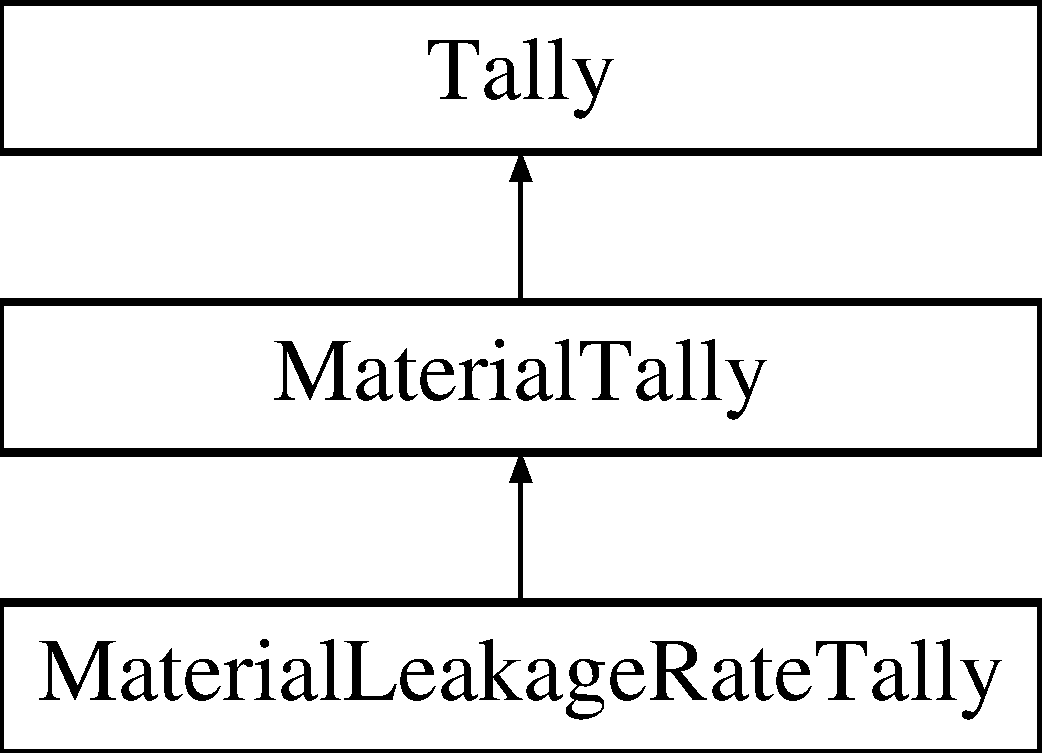
\includegraphics[height=3.000000cm]{classMaterialLeakageRateTally}
\end{center}
\end{figure}
\subsection*{Public Member Functions}
\begin{DoxyCompactItemize}
\item 
\hyperlink{classMaterialLeakageRateTally_af2523d4d3495400bcb0cc94951f4bb43}{Material\-Leakage\-Rate\-Tally} (\hyperlink{classMaterial}{Material} $\ast$material, const char $\ast$tally\-\_\-name=(char $\ast$)\char`\"{}\char`\"{})
\begin{DoxyCompactList}\small\item\em \hyperlink{classMaterialLeakageRateTally}{Material\-Leakage\-Rate\-Tally} constructor calls the \hyperlink{classMaterialTally}{Material\-Tally} constructor and \hyperlink{classTally}{Tally} constructors and sets the tally type to L\-E\-A\-K\-A\-G\-E\-\_\-\-R\-A\-T\-E. \end{DoxyCompactList}\item 
void \hyperlink{classMaterialLeakageRateTally_ad23d9da8c90ce281205d70c3b3132cc3}{tally} (\hyperlink{structneutron}{neutron} $\ast$\hyperlink{structneutron}{neutron})
\begin{DoxyCompactList}\small\item\em \hyperlink{classTally}{Tally} the material leakage rate by incrementing the tally by $ DB^2 $ at the neutron's energy. \end{DoxyCompactList}\end{DoxyCompactItemize}
\subsection*{Additional Inherited Members}


\subsection{Detailed Description}
A class for tallying the leakage rate for the regions filled by a material. 

\subsection{Constructor \& Destructor Documentation}
\hypertarget{classMaterialLeakageRateTally_af2523d4d3495400bcb0cc94951f4bb43}{\index{Material\-Leakage\-Rate\-Tally@{Material\-Leakage\-Rate\-Tally}!Material\-Leakage\-Rate\-Tally@{Material\-Leakage\-Rate\-Tally}}
\index{Material\-Leakage\-Rate\-Tally@{Material\-Leakage\-Rate\-Tally}!MaterialLeakageRateTally@{Material\-Leakage\-Rate\-Tally}}
\subsubsection[{Material\-Leakage\-Rate\-Tally}]{\setlength{\rightskip}{0pt plus 5cm}Material\-Leakage\-Rate\-Tally\-::\-Material\-Leakage\-Rate\-Tally (
\begin{DoxyParamCaption}
\item[{{\bf Material} $\ast$}]{material, }
\item[{const char $\ast$}]{tally\-\_\-name = {\ttfamily (char$\ast$)\char`\"{}\char`\"{}}}
\end{DoxyParamCaption}
)\hspace{0.3cm}{\ttfamily [inline]}}}\label{classMaterialLeakageRateTally_af2523d4d3495400bcb0cc94951f4bb43}


\hyperlink{classMaterialLeakageRateTally}{Material\-Leakage\-Rate\-Tally} constructor calls the \hyperlink{classMaterialTally}{Material\-Tally} constructor and \hyperlink{classTally}{Tally} constructors and sets the tally type to L\-E\-A\-K\-A\-G\-E\-\_\-\-R\-A\-T\-E. 


\begin{DoxyParams}{Parameters}
{\em material} & a pointer to the material within which to tally \\
\hline
{\em tally\-\_\-name} & a character array for the tally name (optional) \\
\hline
\end{DoxyParams}


\subsection{Member Function Documentation}
\hypertarget{classMaterialLeakageRateTally_ad23d9da8c90ce281205d70c3b3132cc3}{\index{Material\-Leakage\-Rate\-Tally@{Material\-Leakage\-Rate\-Tally}!tally@{tally}}
\index{tally@{tally}!MaterialLeakageRateTally@{Material\-Leakage\-Rate\-Tally}}
\subsubsection[{tally}]{\setlength{\rightskip}{0pt plus 5cm}void Material\-Leakage\-Rate\-Tally\-::tally (
\begin{DoxyParamCaption}
\item[{{\bf neutron} $\ast$}]{neutron}
\end{DoxyParamCaption}
)\hspace{0.3cm}{\ttfamily [virtual]}}}\label{classMaterialLeakageRateTally_ad23d9da8c90ce281205d70c3b3132cc3}


\hyperlink{classTally}{Tally} the material leakage rate by incrementing the tally by $ DB^2 $ at the neutron's energy. 


\begin{DoxyParams}{Parameters}
{\em neutron} & the neutron of interest \\
\hline
\end{DoxyParams}


Implements \hyperlink{classMaterialTally_ab2debba62f51212ec8b39b7aeea3f54d}{Material\-Tally}.



The documentation for this class was generated from the following files\-:\begin{DoxyCompactItemize}
\item 
\hyperlink{Tally_8h}{Tally.\-h}\item 
Tally.\-cpp\end{DoxyCompactItemize}

\hypertarget{classMaterialTally}{\section{Material\-Tally Class Reference}
\label{classMaterialTally}\index{Material\-Tally@{Material\-Tally}}
}


An abstract class for tallies with M\-A\-T\-E\-R\-I\-A\-L domain type.  




{\ttfamily \#include \char`\"{}pinspec/src/\-Tally.\-h\char`\"{}}

Inheritance diagram for Material\-Tally\-:\begin{figure}[H]
\begin{center}
\leavevmode
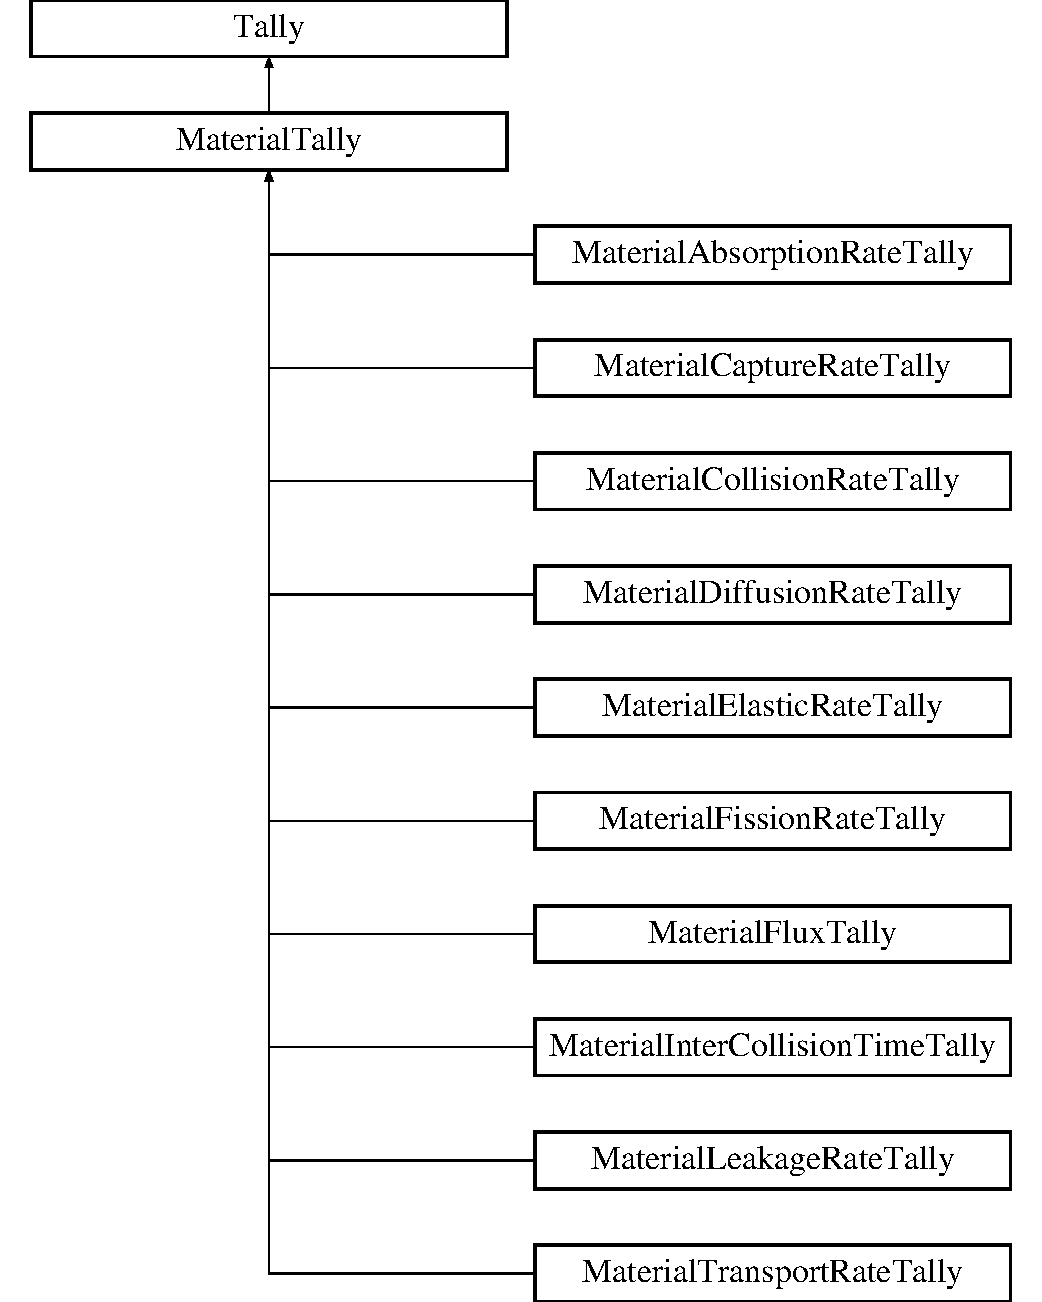
\includegraphics[height=12.000000cm]{classMaterialTally}
\end{center}
\end{figure}
\subsection*{Public Member Functions}
\begin{DoxyCompactItemize}
\item 
\hyperlink{classMaterialTally_a1401be513e221963f200bd241801c4d3}{Material\-Tally} (\hyperlink{classMaterial}{Material} $\ast$material, const char $\ast$tally\-\_\-name=(char $\ast$)\char`\"{}\char`\"{})
\begin{DoxyCompactList}\small\item\em \hyperlink{classMaterialTally}{Material\-Tally} constructor calls the \hyperlink{classTally}{Tally} constructor and sets the tally domain to M\-A\-T\-E\-R\-I\-A\-L. \end{DoxyCompactList}\item 
\hyperlink{classMaterial}{Material} $\ast$ \hyperlink{classMaterialTally_a97f01dd3748be423290db60d3e16d81f}{get\-Material} ()
\begin{DoxyCompactList}\small\item\em Returns the material in which this tally resides. \end{DoxyCompactList}\item 
\hypertarget{classMaterialTally_ab2debba62f51212ec8b39b7aeea3f54d}{virtual void \hyperlink{classMaterialTally_ab2debba62f51212ec8b39b7aeea3f54d}{tally} (\hyperlink{structneutron}{neutron} $\ast$\hyperlink{structneutron}{neutron})=0}\label{classMaterialTally_ab2debba62f51212ec8b39b7aeea3f54d}

\begin{DoxyCompactList}\small\item\em A method to tally a neutron to be implemented by subclasses. \end{DoxyCompactList}\end{DoxyCompactItemize}
\subsection*{Protected Attributes}
\begin{DoxyCompactItemize}
\item 
\hyperlink{classMaterial}{Material} $\ast$ \hyperlink{classMaterialTally_a7dcd60be3a3ccd3631aa2ef1cc3057ec}{\-\_\-material}
\end{DoxyCompactItemize}


\subsection{Detailed Description}
An abstract class for tallies with M\-A\-T\-E\-R\-I\-A\-L domain type. 

A \hyperlink{classMaterialTally}{Material\-Tally} is for tallying within a material. The \hyperlink{classMaterialTally}{Material\-Tally} is an abstract class and must be implemented for each tally\-Type. 

\subsection{Constructor \& Destructor Documentation}
\hypertarget{classMaterialTally_a1401be513e221963f200bd241801c4d3}{\index{Material\-Tally@{Material\-Tally}!Material\-Tally@{Material\-Tally}}
\index{Material\-Tally@{Material\-Tally}!MaterialTally@{Material\-Tally}}
\subsubsection[{Material\-Tally}]{\setlength{\rightskip}{0pt plus 5cm}Material\-Tally\-::\-Material\-Tally (
\begin{DoxyParamCaption}
\item[{{\bf Material} $\ast$}]{material, }
\item[{const char $\ast$}]{tally\-\_\-name = {\ttfamily (char$\ast$)\char`\"{}\char`\"{}}}
\end{DoxyParamCaption}
)\hspace{0.3cm}{\ttfamily [inline]}}}\label{classMaterialTally_a1401be513e221963f200bd241801c4d3}


\hyperlink{classMaterialTally}{Material\-Tally} constructor calls the \hyperlink{classTally}{Tally} constructor and sets the tally domain to M\-A\-T\-E\-R\-I\-A\-L. 


\begin{DoxyParams}{Parameters}
{\em material} & a pointer to the material within which to tally \\
\hline
{\em tally\-\_\-name} & a character array for the tally name (optional) \\
\hline
\end{DoxyParams}


\subsection{Member Function Documentation}
\hypertarget{classMaterialTally_a97f01dd3748be423290db60d3e16d81f}{\index{Material\-Tally@{Material\-Tally}!get\-Material@{get\-Material}}
\index{get\-Material@{get\-Material}!MaterialTally@{Material\-Tally}}
\subsubsection[{get\-Material}]{\setlength{\rightskip}{0pt plus 5cm}{\bf Material}$\ast$ Material\-Tally\-::get\-Material (
\begin{DoxyParamCaption}
{}
\end{DoxyParamCaption}
)\hspace{0.3cm}{\ttfamily [inline]}}}\label{classMaterialTally_a97f01dd3748be423290db60d3e16d81f}


Returns the material in which this tally resides. 

\begin{DoxyReturn}{Returns}
a pointer to the material 
\end{DoxyReturn}


\subsection{Member Data Documentation}
\hypertarget{classMaterialTally_a7dcd60be3a3ccd3631aa2ef1cc3057ec}{\index{Material\-Tally@{Material\-Tally}!\-\_\-material@{\-\_\-material}}
\index{\-\_\-material@{\-\_\-material}!MaterialTally@{Material\-Tally}}
\subsubsection[{\-\_\-material}]{\setlength{\rightskip}{0pt plus 5cm}{\bf Material}$\ast$ Material\-Tally\-::\-\_\-material\hspace{0.3cm}{\ttfamily [protected]}}}\label{classMaterialTally_a7dcd60be3a3ccd3631aa2ef1cc3057ec}
A pointer to the material in which this tally resides 

The documentation for this class was generated from the following file\-:\begin{DoxyCompactItemize}
\item 
\hyperlink{Tally_8h}{Tally.\-h}\end{DoxyCompactItemize}

\hypertarget{classMaterialTransportRateTally}{\section{Material\-Transport\-Rate\-Tally Class Reference}
\label{classMaterialTransportRateTally}\index{Material\-Transport\-Rate\-Tally@{Material\-Transport\-Rate\-Tally}}
}


A class for tallying the transport rate within a material.  




{\ttfamily \#include \char`\"{}pinspec/src/\-Tally.\-h\char`\"{}}

Inheritance diagram for Material\-Transport\-Rate\-Tally\-:\begin{figure}[H]
\begin{center}
\leavevmode
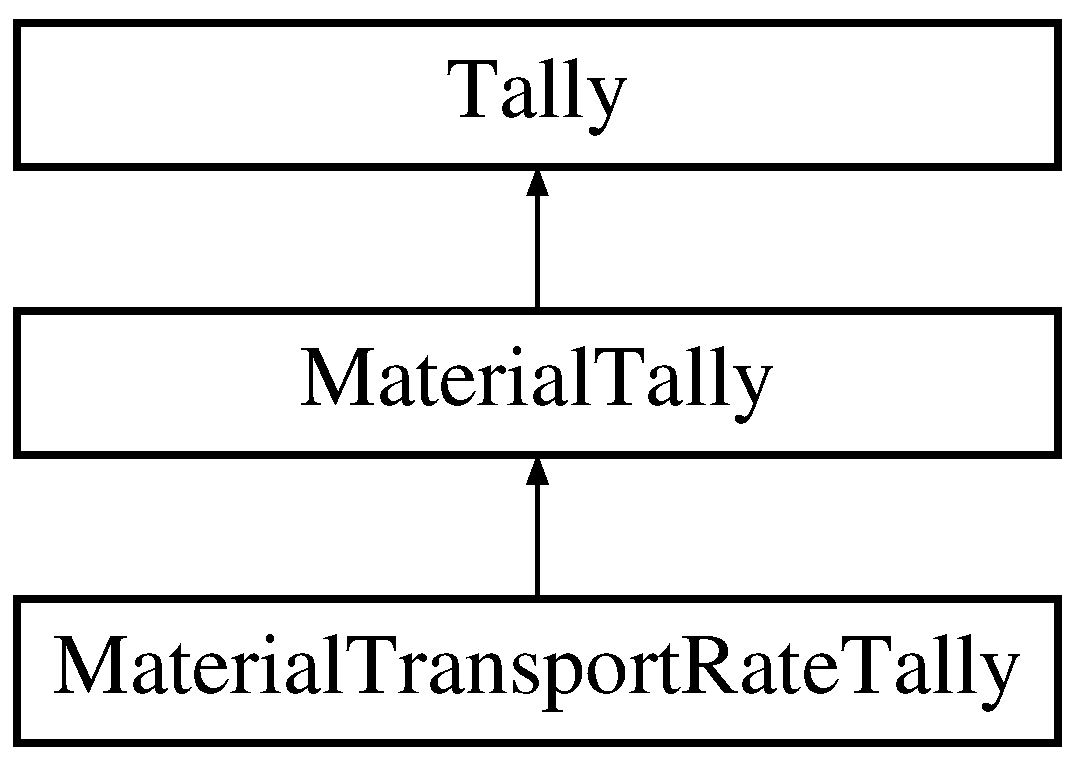
\includegraphics[height=3.000000cm]{classMaterialTransportRateTally}
\end{center}
\end{figure}
\subsection*{Public Member Functions}
\begin{DoxyCompactItemize}
\item 
\hyperlink{classMaterialTransportRateTally_afbb8c05e018128d52093e615cadf1b1d}{Material\-Transport\-Rate\-Tally} (\hyperlink{classMaterial}{Material} $\ast$material, const char $\ast$tally\-\_\-name=(char $\ast$)\char`\"{}\char`\"{})
\begin{DoxyCompactList}\small\item\em \hyperlink{classMaterialTransportRateTally}{Material\-Transport\-Rate\-Tally} constructor calls the \hyperlink{classMaterialTally}{Material\-Tally} constructor and \hyperlink{classTally}{Tally} constructors and sets the tally type to T\-R\-A\-N\-S\-P\-O\-R\-T\-\_\-\-R\-A\-T\-E. \end{DoxyCompactList}\item 
void \hyperlink{classMaterialTransportRateTally_a10c3aa96348177a1002395295d51c90a}{tally} (\hyperlink{structneutron}{neutron} $\ast$\hyperlink{structneutron}{neutron})
\begin{DoxyCompactList}\small\item\em \hyperlink{classTally}{Tally} the material transport rate by incrementing the tally by $ \frac{\Sigma_tr}{\Sigma_t} $ at the neutron's energy. \end{DoxyCompactList}\end{DoxyCompactItemize}
\subsection*{Additional Inherited Members}


\subsection{Detailed Description}
A class for tallying the transport rate within a material. 

\subsection{Constructor \& Destructor Documentation}
\hypertarget{classMaterialTransportRateTally_afbb8c05e018128d52093e615cadf1b1d}{\index{Material\-Transport\-Rate\-Tally@{Material\-Transport\-Rate\-Tally}!Material\-Transport\-Rate\-Tally@{Material\-Transport\-Rate\-Tally}}
\index{Material\-Transport\-Rate\-Tally@{Material\-Transport\-Rate\-Tally}!MaterialTransportRateTally@{Material\-Transport\-Rate\-Tally}}
\subsubsection[{Material\-Transport\-Rate\-Tally}]{\setlength{\rightskip}{0pt plus 5cm}Material\-Transport\-Rate\-Tally\-::\-Material\-Transport\-Rate\-Tally (
\begin{DoxyParamCaption}
\item[{{\bf Material} $\ast$}]{material, }
\item[{const char $\ast$}]{tally\-\_\-name = {\ttfamily (char$\ast$)\char`\"{}\char`\"{}}}
\end{DoxyParamCaption}
)\hspace{0.3cm}{\ttfamily [inline]}}}\label{classMaterialTransportRateTally_afbb8c05e018128d52093e615cadf1b1d}


\hyperlink{classMaterialTransportRateTally}{Material\-Transport\-Rate\-Tally} constructor calls the \hyperlink{classMaterialTally}{Material\-Tally} constructor and \hyperlink{classTally}{Tally} constructors and sets the tally type to T\-R\-A\-N\-S\-P\-O\-R\-T\-\_\-\-R\-A\-T\-E. 


\begin{DoxyParams}{Parameters}
{\em material} & a pointer to the material within which to tally \\
\hline
{\em tally\-\_\-name} & a character array for the tally name (optional) \\
\hline
\end{DoxyParams}


\subsection{Member Function Documentation}
\hypertarget{classMaterialTransportRateTally_a10c3aa96348177a1002395295d51c90a}{\index{Material\-Transport\-Rate\-Tally@{Material\-Transport\-Rate\-Tally}!tally@{tally}}
\index{tally@{tally}!MaterialTransportRateTally@{Material\-Transport\-Rate\-Tally}}
\subsubsection[{tally}]{\setlength{\rightskip}{0pt plus 5cm}void Material\-Transport\-Rate\-Tally\-::tally (
\begin{DoxyParamCaption}
\item[{{\bf neutron} $\ast$}]{neutron}
\end{DoxyParamCaption}
)\hspace{0.3cm}{\ttfamily [virtual]}}}\label{classMaterialTransportRateTally_a10c3aa96348177a1002395295d51c90a}


\hyperlink{classTally}{Tally} the material transport rate by incrementing the tally by $ \frac{\Sigma_tr}{\Sigma_t} $ at the neutron's energy. 


\begin{DoxyParams}{Parameters}
{\em neutron} & the neutron of interest \\
\hline
\end{DoxyParams}


Implements \hyperlink{classMaterialTally_ab2debba62f51212ec8b39b7aeea3f54d}{Material\-Tally}.



The documentation for this class was generated from the following files\-:\begin{DoxyCompactItemize}
\item 
\hyperlink{Tally_8h}{Tally.\-h}\item 
Tally.\-cpp\end{DoxyCompactItemize}

\hypertarget{structneutron}{\section{neutron Struct Reference}
\label{structneutron}\index{neutron@{neutron}}
}


Represents a neutron in a P\-I\-N\-S\-P\-E\-C simulation.  




{\ttfamily \#include $<$Neutron.\-h$>$}

\subsection*{Public Attributes}
\begin{DoxyCompactItemize}
\item 
int \hyperlink{structneutron_a0fc51df4fbcc6f41460e937a1f63ead2}{\-\_\-batch\-\_\-num}
\item 
float \hyperlink{structneutron_a14743394ac7bf443a57bccf9ab8beba5}{\-\_\-x}
\item 
float \hyperlink{structneutron_a9bc73caa5e8ea77020e7112299deec2e}{\-\_\-y}
\item 
float \hyperlink{structneutron_a8ee10b15ab1dc8294c84a0d742e15154}{\-\_\-z}
\item 
float \hyperlink{structneutron_a4ac5f314a0547708378d6b00a8863af0}{\-\_\-u}
\item 
float \hyperlink{structneutron_a382ebb7a5a3c7b971b283f0eb2e14ea6}{\-\_\-v}
\item 
float \hyperlink{structneutron_a2556e63540e62a318ca919cbe24f9794}{\-\_\-w}
\item 
float \hyperlink{structneutron_ad0addd2c6b874a54d838455358e7f6e8}{\-\_\-mu}
\item 
float \hyperlink{structneutron_ac17d30fc4c24666fcab05fe3d787b32d}{\-\_\-phi}
\item 
float \hyperlink{structneutron_a49d28706c0f2d9f3215fdf6da4e89f41}{\-\_\-energy}
\item 
bool \hyperlink{structneutron_ad3765df09268634efd4ff2107e3d150b}{\-\_\-alive}
\item 
\hyperlink{classRegion}{Region} $\ast$ \hyperlink{structneutron_ae09eb9ff92ce5578e2e683bc27e61e3b}{\-\_\-region}
\item 
\hyperlink{classMaterial}{Material} $\ast$ \hyperlink{structneutron_a7af200a58de9f8c535c1247053f70872}{\-\_\-material}
\item 
\hyperlink{classIsotope}{Isotope} $\ast$ \hyperlink{structneutron_a71574f549781c314902596d3ac4da58a}{\-\_\-isotope}
\item 
float \hyperlink{structneutron_a7f4a5f782cd613aed5b7832a198ffce2}{\-\_\-old\-\_\-energy}
\item 
float \hyperlink{structneutron_aac01f1ff8efae019839d37bb959fa33f}{\-\_\-total\-\_\-xs}
\end{DoxyCompactItemize}


\subsection{Detailed Description}
Represents a neutron in a P\-I\-N\-S\-P\-E\-C simulation. 

The neutron struct is the fundamental unit of data needed to represent a neutron in a P\-I\-N\-S\-P\-E\-C simulation. This struct is useful for passing a neutron from object to object, such as from the \hyperlink{classGeometry}{Geometry} to a \hyperlink{classRegion}{Region} to a \hyperlink{classMaterial}{Material} and to an \hyperlink{classIsotope}{Isotope} to update the neutron's energy from a collision. 

\subsection{Member Data Documentation}
\hypertarget{structneutron_ad3765df09268634efd4ff2107e3d150b}{\index{neutron@{neutron}!\-\_\-alive@{\-\_\-alive}}
\index{\-\_\-alive@{\-\_\-alive}!neutron@{neutron}}
\subsubsection[{\-\_\-alive}]{\setlength{\rightskip}{0pt plus 5cm}bool neutron\-::\-\_\-alive}}\label{structneutron_ad3765df09268634efd4ff2107e3d150b}
a boolean representing whether this neutron has been absorbed or not \hypertarget{structneutron_a0fc51df4fbcc6f41460e937a1f63ead2}{\index{neutron@{neutron}!\-\_\-batch\-\_\-num@{\-\_\-batch\-\_\-num}}
\index{\-\_\-batch\-\_\-num@{\-\_\-batch\-\_\-num}!neutron@{neutron}}
\subsubsection[{\-\_\-batch\-\_\-num}]{\setlength{\rightskip}{0pt plus 5cm}int neutron\-::\-\_\-batch\-\_\-num}}\label{structneutron_a0fc51df4fbcc6f41460e937a1f63ead2}
this neutron's batch number in the simulation \hypertarget{structneutron_a49d28706c0f2d9f3215fdf6da4e89f41}{\index{neutron@{neutron}!\-\_\-energy@{\-\_\-energy}}
\index{\-\_\-energy@{\-\_\-energy}!neutron@{neutron}}
\subsubsection[{\-\_\-energy}]{\setlength{\rightskip}{0pt plus 5cm}float neutron\-::\-\_\-energy}}\label{structneutron_a49d28706c0f2d9f3215fdf6da4e89f41}
the neutron's energy in e\-V following its most recent collision \hypertarget{structneutron_a71574f549781c314902596d3ac4da58a}{\index{neutron@{neutron}!\-\_\-isotope@{\-\_\-isotope}}
\index{\-\_\-isotope@{\-\_\-isotope}!neutron@{neutron}}
\subsubsection[{\-\_\-isotope}]{\setlength{\rightskip}{0pt plus 5cm}{\bf Isotope}$\ast$ neutron\-::\-\_\-isotope}}\label{structneutron_a71574f549781c314902596d3ac4da58a}
a pointer to the \hyperlink{classIsotope}{Isotope} with which the neutron most recently collided \hypertarget{structneutron_a7af200a58de9f8c535c1247053f70872}{\index{neutron@{neutron}!\-\_\-material@{\-\_\-material}}
\index{\-\_\-material@{\-\_\-material}!neutron@{neutron}}
\subsubsection[{\-\_\-material}]{\setlength{\rightskip}{0pt plus 5cm}{\bf Material}$\ast$ neutron\-::\-\_\-material}}\label{structneutron_a7af200a58de9f8c535c1247053f70872}
a pointer to the \hyperlink{classMaterial}{Material} with which the neutron most recently collided \hypertarget{structneutron_ad0addd2c6b874a54d838455358e7f6e8}{\index{neutron@{neutron}!\-\_\-mu@{\-\_\-mu}}
\index{\-\_\-mu@{\-\_\-mu}!neutron@{neutron}}
\subsubsection[{\-\_\-mu}]{\setlength{\rightskip}{0pt plus 5cm}float neutron\-::\-\_\-mu}}\label{structneutron_ad0addd2c6b874a54d838455358e7f6e8}
the cosine of the polar angle $\theta$ of this neutron's direction vector\-: $\mu = cos(\theta)$ \hypertarget{structneutron_a7f4a5f782cd613aed5b7832a198ffce2}{\index{neutron@{neutron}!\-\_\-old\-\_\-energy@{\-\_\-old\-\_\-energy}}
\index{\-\_\-old\-\_\-energy@{\-\_\-old\-\_\-energy}!neutron@{neutron}}
\subsubsection[{\-\_\-old\-\_\-energy}]{\setlength{\rightskip}{0pt plus 5cm}float neutron\-::\-\_\-old\-\_\-energy}}\label{structneutron_a7f4a5f782cd613aed5b7832a198ffce2}
the neutron's energy in e\-V prior to its most recent collision \hypertarget{structneutron_ac17d30fc4c24666fcab05fe3d787b32d}{\index{neutron@{neutron}!\-\_\-phi@{\-\_\-phi}}
\index{\-\_\-phi@{\-\_\-phi}!neutron@{neutron}}
\subsubsection[{\-\_\-phi}]{\setlength{\rightskip}{0pt plus 5cm}float neutron\-::\-\_\-phi}}\label{structneutron_ac17d30fc4c24666fcab05fe3d787b32d}
the azimuthal angle $\phi$ of this neutron's direction vector in the xy-\/plane \hypertarget{structneutron_ae09eb9ff92ce5578e2e683bc27e61e3b}{\index{neutron@{neutron}!\-\_\-region@{\-\_\-region}}
\index{\-\_\-region@{\-\_\-region}!neutron@{neutron}}
\subsubsection[{\-\_\-region}]{\setlength{\rightskip}{0pt plus 5cm}{\bf Region}$\ast$ neutron\-::\-\_\-region}}\label{structneutron_ae09eb9ff92ce5578e2e683bc27e61e3b}
a pointer to the Regon in which the neutron most recently collided \hypertarget{structneutron_aac01f1ff8efae019839d37bb959fa33f}{\index{neutron@{neutron}!\-\_\-total\-\_\-xs@{\-\_\-total\-\_\-xs}}
\index{\-\_\-total\-\_\-xs@{\-\_\-total\-\_\-xs}!neutron@{neutron}}
\subsubsection[{\-\_\-total\-\_\-xs}]{\setlength{\rightskip}{0pt plus 5cm}float neutron\-::\-\_\-total\-\_\-xs}}\label{structneutron_aac01f1ff8efae019839d37bb959fa33f}
the total macroscopic cross-\/section in $cm^{-1}$ of the material in which the neutron collided at its collision energy \hypertarget{structneutron_a4ac5f314a0547708378d6b00a8863af0}{\index{neutron@{neutron}!\-\_\-u@{\-\_\-u}}
\index{\-\_\-u@{\-\_\-u}!neutron@{neutron}}
\subsubsection[{\-\_\-u}]{\setlength{\rightskip}{0pt plus 5cm}float neutron\-::\-\_\-u}}\label{structneutron_a4ac5f314a0547708378d6b00a8863af0}
the component of this neutron's velocity unit vector along the x-\/axis \hypertarget{structneutron_a382ebb7a5a3c7b971b283f0eb2e14ea6}{\index{neutron@{neutron}!\-\_\-v@{\-\_\-v}}
\index{\-\_\-v@{\-\_\-v}!neutron@{neutron}}
\subsubsection[{\-\_\-v}]{\setlength{\rightskip}{0pt plus 5cm}float neutron\-::\-\_\-v}}\label{structneutron_a382ebb7a5a3c7b971b283f0eb2e14ea6}
the component of this neutron's velocity unit vector along the y-\/axis \hypertarget{structneutron_a2556e63540e62a318ca919cbe24f9794}{\index{neutron@{neutron}!\-\_\-w@{\-\_\-w}}
\index{\-\_\-w@{\-\_\-w}!neutron@{neutron}}
\subsubsection[{\-\_\-w}]{\setlength{\rightskip}{0pt plus 5cm}float neutron\-::\-\_\-w}}\label{structneutron_a2556e63540e62a318ca919cbe24f9794}
the component of this neutron's velocity unit vector along the z-\/axis \hypertarget{structneutron_a14743394ac7bf443a57bccf9ab8beba5}{\index{neutron@{neutron}!\-\_\-x@{\-\_\-x}}
\index{\-\_\-x@{\-\_\-x}!neutron@{neutron}}
\subsubsection[{\-\_\-x}]{\setlength{\rightskip}{0pt plus 5cm}float neutron\-::\-\_\-x}}\label{structneutron_a14743394ac7bf443a57bccf9ab8beba5}
the x-\/coordinate of this neutron's location \hypertarget{structneutron_a9bc73caa5e8ea77020e7112299deec2e}{\index{neutron@{neutron}!\-\_\-y@{\-\_\-y}}
\index{\-\_\-y@{\-\_\-y}!neutron@{neutron}}
\subsubsection[{\-\_\-y}]{\setlength{\rightskip}{0pt plus 5cm}float neutron\-::\-\_\-y}}\label{structneutron_a9bc73caa5e8ea77020e7112299deec2e}
the y-\/coordinate of this neutron's location \hypertarget{structneutron_a8ee10b15ab1dc8294c84a0d742e15154}{\index{neutron@{neutron}!\-\_\-z@{\-\_\-z}}
\index{\-\_\-z@{\-\_\-z}!neutron@{neutron}}
\subsubsection[{\-\_\-z}]{\setlength{\rightskip}{0pt plus 5cm}float neutron\-::\-\_\-z}}\label{structneutron_a8ee10b15ab1dc8294c84a0d742e15154}
the z-\/coordinate of this neutron's location 

The documentation for this struct was generated from the following file\-:\begin{DoxyCompactItemize}
\item 
\hyperlink{Neutron_8h}{Neutron.\-h}\end{DoxyCompactItemize}

\hypertarget{classRegion}{\section{Region Class Reference}
\label{classRegion}\index{Region@{Region}}
}


The region class represents a region in 2\-D space.  




{\ttfamily \#include \char`\"{}src/pinspec/\-Region.\-h\char`\"{}}

\subsection*{Public Member Functions}
\begin{DoxyCompactItemize}
\item 
\hyperlink{classRegion_ab0d1873c68539b5339811f413ecb4dbb}{Region} (char $\ast$region\-\_\-name, \hyperlink{Region_8h_a2c25b4a3d851e2d45d7a435a73598323}{region\-Type} type)
\begin{DoxyCompactList}\small\item\em \hyperlink{classRegion}{Region} constructor. \end{DoxyCompactList}\item 
virtual \hyperlink{classRegion_a3c3670fff78f7511d156e3b2f0bc6266}{$\sim$\-Region} ()
\begin{DoxyCompactList}\small\item\em \hyperlink{classRegion}{Region} destructor. \end{DoxyCompactList}\item 
char $\ast$ \hyperlink{classRegion_abac6cb4d426f59e3b4b3f7a5ef8f4a1d}{get\-Region\-Name} ()
\begin{DoxyCompactList}\small\item\em Return the name of the region. \end{DoxyCompactList}\item 
float \hyperlink{classRegion_a2c3eca3c5373770e19d36198859f4ccb}{get\-Volume} ()
\begin{DoxyCompactList}\small\item\em returns the volume of this \hyperlink{classRegion}{Region} $ (cm^3) $. \end{DoxyCompactList}\item 
\hyperlink{classMaterial}{Material} $\ast$ \hyperlink{classRegion_ace26edc725e1f4d723964f3961e65ceb}{get\-Material} ()
\begin{DoxyCompactList}\small\item\em Returns a pointer to the material filling this region. \end{DoxyCompactList}\item 
bool \hyperlink{classRegion_a46eb443386a0f3003a28772f78e6de70}{contains\-Isotope} (\hyperlink{classIsotope}{Isotope} $\ast$isotope)
\begin{DoxyCompactList}\small\item\em Determines whether this region contains a particular isotope. \end{DoxyCompactList}\item 
\hyperlink{Region_8h_a2c25b4a3d851e2d45d7a435a73598323}{region\-Type} \hyperlink{classRegion_a79ac377684286e49a7ae54c5543c909c}{get\-Region\-Type} ()
\begin{DoxyCompactList}\small\item\em Return the type of region. \end{DoxyCompactList}\item 
bool \hyperlink{classRegion_a28071086d54cd10656a7dd887a9b7d7b}{is\-Fuel} ()
\begin{DoxyCompactList}\small\item\em Returns true if this region is the fuel, false otherwise. \end{DoxyCompactList}\item 
bool \hyperlink{classRegion_a07b3de22a98396471732b5a06478a2b6}{is\-Moderator} ()
\begin{DoxyCompactList}\small\item\em Returns true if this region is the moderator, false otherwise. \end{DoxyCompactList}\item 
bool \hyperlink{classRegion_a32c33d47e4cf99a839a7ea36c1f91b73}{is\-Infinite} ()
\begin{DoxyCompactList}\small\item\em Returns true if this region is an infnite medium, false otherwise. \end{DoxyCompactList}\item 
float \hyperlink{classRegion_a1eece240d2a03c92abd79c3fcb708fa1}{get\-Fuel\-Radius} ()
\begin{DoxyCompactList}\small\item\em Returns the fuel pin radius if not an I\-N\-F\-I\-N\-I\-T\-E region type. \end{DoxyCompactList}\item 
float \hyperlink{classRegion_a06dcc9cfe0a9d07594ad4baae3f426b9}{get\-Pitch} ()
\begin{DoxyCompactList}\small\item\em Returns the pin cell pitch if not an I\-N\-F\-I\-N\-I\-T\-E region type. \end{DoxyCompactList}\item 
float \hyperlink{classRegion_a032f38b6fbd2bac296aff6367a273456}{get\-Buckling\-Squared} ()
\begin{DoxyCompactList}\small\item\em Returns the squared geometric buckling. \end{DoxyCompactList}\item 
float \hyperlink{classRegion_a44ae74637def12405bf79097854ce376}{get\-Total\-Macro\-X\-S} (float energy)
\begin{DoxyCompactList}\small\item\em Computes and returns the total macroscopic cross-\/section in the region at some energy (e\-V). \end{DoxyCompactList}\item 
float \hyperlink{classRegion_a1e0b264433131ab0e902d9fc2fee7477}{get\-Total\-Macro\-X\-S} (int energy\-\_\-index)
\begin{DoxyCompactList}\small\item\em Computes and returns the total macroscopic cross-\/section in the region at some index into the uniform lethargy grid. \end{DoxyCompactList}\item 
float \hyperlink{classRegion_a0b51ec68621a1861e9ed5e13e5824b3c}{get\-Total\-Micro\-X\-S} (float energy)
\begin{DoxyCompactList}\small\item\em Computes and returns the total microscopic cross-\/section in the region at some energy (e\-V). \end{DoxyCompactList}\item 
float \hyperlink{classRegion_acc45e5ac87b7892b02df8624aafbb5b7}{get\-Total\-Micro\-X\-S} (int energy\-\_\-index)
\begin{DoxyCompactList}\small\item\em Computes and returns the total microscopic cross-\/section in the region at some index into the uniform lethargy grid. \end{DoxyCompactList}\item 
float \hyperlink{classRegion_a90a6edf5bbe9d55ccb6c326af430dade}{get\-Elastic\-Macro\-X\-S} (float energy)
\begin{DoxyCompactList}\small\item\em Computes and returns the macroscopic elastic scattering cross-\/section in the region at some energy (e\-V). \end{DoxyCompactList}\item 
float \hyperlink{classRegion_a886c0cb8cefaa51c6b9166c7c7eb017f}{get\-Elastic\-Macro\-X\-S} (int energy\-\_\-index)
\begin{DoxyCompactList}\small\item\em Computes and returns the macroscopic elastic scattering cross-\/section in the region at some index into the uniform lethargy grid. \end{DoxyCompactList}\item 
float \hyperlink{classRegion_a481bb2ea17d504a72a37c46d3a54acbb}{get\-Elastic\-Micro\-X\-S} (float energy)
\begin{DoxyCompactList}\small\item\em Computes and returns the microscopic elastic scattering cross-\/section in the region at some energy (e\-V). \end{DoxyCompactList}\item 
float \hyperlink{classRegion_a933559a825a28f29adfdfe3f592d34bd}{get\-Elastic\-Micro\-X\-S} (int energy\-\_\-index)
\begin{DoxyCompactList}\small\item\em Computes and returns the microscopic elastic scattering cross-\/section in the region at some index into the uniform lethargy grid. \end{DoxyCompactList}\item 
float \hyperlink{classRegion_a5bdd08baa4b621e7ed540438d8624cb7}{get\-Absorption\-Macro\-X\-S} (float energy)
\begin{DoxyCompactList}\small\item\em Computes and returns the macroscopic absorption cross-\/section in the region at energy (e\-V). \end{DoxyCompactList}\item 
float \hyperlink{classRegion_ae7a0fe8576783dfa724e8db9dd2e1365}{get\-Absorption\-Macro\-X\-S} (int energy\-\_\-index)
\begin{DoxyCompactList}\small\item\em Computes and returns the macroscopic absorption cross-\/section in the region at some index into the uniform lethargy grid. \end{DoxyCompactList}\item 
float \hyperlink{classRegion_a96446c70b8fe96ceffc301c7589c152b}{get\-Absorption\-Micro\-X\-S} (float energy)
\begin{DoxyCompactList}\small\item\em Computes and returns the microscopic absorption cross-\/section in the region at some energy (e\-V). \end{DoxyCompactList}\item 
float \hyperlink{classRegion_aa040e637f1ff6819547c0e4c0a74c4ff}{get\-Absorption\-Micro\-X\-S} (int energy\-\_\-index)
\begin{DoxyCompactList}\small\item\em Computes and returns the microscopic absorption cross-\/section in the region at some index into the uniform lethargy grid. \end{DoxyCompactList}\item 
float \hyperlink{classRegion_a1bb6d0746ee525b5c456bd3b4d5c4cd2}{get\-Capture\-Macro\-X\-S} (float energy)
\begin{DoxyCompactList}\small\item\em Computes and returns the macroscopic capture cross-\/section in the region at some energy (e\-V). \end{DoxyCompactList}\item 
float \hyperlink{classRegion_a646683114e40ca729efbf8e0a80eb615}{get\-Capture\-Macro\-X\-S} (int energy\-\_\-index)
\begin{DoxyCompactList}\small\item\em Computes and returns the macroscopic capture cross-\/section in the region at some index into the uniform lethargy grid. \end{DoxyCompactList}\item 
float \hyperlink{classRegion_ac84f7469d2f314f696d51efd9f661351}{get\-Capture\-Micro\-X\-S} (float energy)
\begin{DoxyCompactList}\small\item\em Computes and returns the microscopic capture cross-\/section in the region at some energy (e\-V). \end{DoxyCompactList}\item 
float \hyperlink{classRegion_aed259d162d731367523beecc8bd85029}{get\-Capture\-Micro\-X\-S} (int energy\-\_\-index)
\begin{DoxyCompactList}\small\item\em Computes and returns the microscopic capture cross-\/section in the region at some index into the uniform lethargy grid. \end{DoxyCompactList}\item 
float \hyperlink{classRegion_a3bbfdb7b952c065e8c940e1d42df6884}{get\-Fission\-Macro\-X\-S} (float energy)
\begin{DoxyCompactList}\small\item\em Computes and returns the macroscopic fission cross-\/section in the region at some energy (e\-V). \end{DoxyCompactList}\item 
float \hyperlink{classRegion_a92df554bce8ad1fc5779d4b4f0d1329a}{get\-Fission\-Macro\-X\-S} (int energy\-\_\-index)
\begin{DoxyCompactList}\small\item\em Computes and returns the macroscopic fission cross-\/section in the region at some index into the uniform lethargy grid. \end{DoxyCompactList}\item 
float \hyperlink{classRegion_ac752b2a3eef8f5d5a1003f5f5b6bdf89}{get\-Fission\-Micro\-X\-S} (float energy)
\begin{DoxyCompactList}\small\item\em Computes and returns the microscopic fission cross-\/section in the region at some energy (e\-V) \end{DoxyCompactList}\item 
float \hyperlink{classRegion_a93a93182c14494e09a35bfda54a0cebd}{get\-Fission\-Micro\-X\-S} (int energy\-\_\-index)
\begin{DoxyCompactList}\small\item\em Computes and returns the microscopic fission cross-\/section in the region at some index into the uniform lethargy grid. \end{DoxyCompactList}\item 
float \hyperlink{classRegion_a5945faaec979b87aaf2b673ac240cc7d}{get\-Transport\-Micro\-X\-S} (float energy)
\begin{DoxyCompactList}\small\item\em Computes and returns the microscopic transport cross-\/section in the region at some index into the uniform lethargy grid. \end{DoxyCompactList}\item 
float \hyperlink{classRegion_abd82a6bf83979583bfbf15b47e4e9a25}{get\-Transport\-Micro\-X\-S} (int energy\-\_\-index)
\begin{DoxyCompactList}\small\item\em Computes and returns the microscopic transport cross-\/section in the region at some index into the uniform lethargy grid. \end{DoxyCompactList}\item 
float \hyperlink{classRegion_a7f26efd91c1fd8ab53c14f48db5ba236}{get\-Transport\-Macro\-X\-S} (float energy)
\begin{DoxyCompactList}\small\item\em Computes and returns the macroscopic transport cross-\/section in the region at some index into the uniform lethargy grid. \end{DoxyCompactList}\item 
float \hyperlink{classRegion_a5c7da29f8103f2b754d5ff830d2d5573}{get\-Transport\-Macro\-X\-S} (int energy\-\_\-index)
\begin{DoxyCompactList}\small\item\em Computes and returns the macroscopic transport cross-\/section in the region at some index into the uniform lethargy grid. \end{DoxyCompactList}\item 
void \hyperlink{classRegion_a7db7e7d177ab05b9142300181f261f80}{set\-Material} (\hyperlink{classMaterial}{Material} $\ast$material)
\begin{DoxyCompactList}\small\item\em Set the material filling this region. \end{DoxyCompactList}\item 
void \hyperlink{classRegion_aeaaceb598753fb4001bbb9f9ab2e475c}{set\-Fuel\-Radius} (float radius)
\begin{DoxyCompactList}\small\item\em Sets the fuel radius if the region is not of I\-N\-F\-I\-N\-I\-T\-E type. \end{DoxyCompactList}\item 
void \hyperlink{classRegion_a59684ee41c0461555b53688023d16f3f}{set\-Pitch} (float pitch)
\begin{DoxyCompactList}\small\item\em Sets the pin cell pitch if the region is not of I\-N\-F\-I\-N\-I\-T\-E type. \end{DoxyCompactList}\item 
void \hyperlink{classRegion_aaf17e980febbd4856c884d288922f8b6}{set\-Volume} (float volume)
\begin{DoxyCompactList}\small\item\em Sets the volume for this region $ (cm^3) $. \end{DoxyCompactList}\item 
void \hyperlink{classRegion_afeed8677dff0c9fe1eefae1fb9acd66c}{set\-Buckling\-Squared} (float buckling\-\_\-squared)
\begin{DoxyCompactList}\small\item\em Sets the squared geometric buckling for the geometry. \end{DoxyCompactList}\item 
void \hyperlink{classRegion_aa1dcade90f26be22436ce940f22b5b32}{collide\-Neutron} (\hyperlink{structneutron}{neutron} $\ast$\hyperlink{structneutron}{neutron})
\begin{DoxyCompactList}\small\item\em This method collides a neutron within the region. \end{DoxyCompactList}\end{DoxyCompactItemize}


\subsection{Detailed Description}
The region class represents a region in 2\-D space. 

The region class is a superclass allowing for subclasses representing infinited media, heterogeneous/homogeneous equivalance fuel/moderator regions, or even heterogeneous regions bounded by 2\-D quadratic surfaces, filled by a material. 

\subsection{Constructor \& Destructor Documentation}
\hypertarget{classRegion_ab0d1873c68539b5339811f413ecb4dbb}{\index{Region@{Region}!Region@{Region}}
\index{Region@{Region}!Region@{Region}}
\subsubsection[{Region}]{\setlength{\rightskip}{0pt plus 5cm}Region\-::\-Region (
\begin{DoxyParamCaption}
\item[{char $\ast$}]{region\-\_\-name, }
\item[{{\bf region\-Type}}]{type}
\end{DoxyParamCaption}
)}}\label{classRegion_ab0d1873c68539b5339811f413ecb4dbb}


\hyperlink{classRegion}{Region} constructor. 

Sets defaults for the geometric parameters to 0. 
\begin{DoxyParams}{Parameters}
{\em region\-\_\-name} & the name of the region \\
\hline
{\em type} & the type region (I\-N\-F\-I\-N\-I\-T\-E, F\-U\-E\-L, etc) \\
\hline
\end{DoxyParams}
\hypertarget{classRegion_a3c3670fff78f7511d156e3b2f0bc6266}{\index{Region@{Region}!$\sim$\-Region@{$\sim$\-Region}}
\index{$\sim$\-Region@{$\sim$\-Region}!Region@{Region}}
\subsubsection[{$\sim$\-Region}]{\setlength{\rightskip}{0pt plus 5cm}Region\-::$\sim$\-Region (
\begin{DoxyParamCaption}
{}
\end{DoxyParamCaption}
)\hspace{0.3cm}{\ttfamily [virtual]}}}\label{classRegion_a3c3670fff78f7511d156e3b2f0bc6266}


\hyperlink{classRegion}{Region} destructor. 

The destructor does not delete anything since S\-W\-I\-G deals with garbage collection. 

\subsection{Member Function Documentation}
\hypertarget{classRegion_aa1dcade90f26be22436ce940f22b5b32}{\index{Region@{Region}!collide\-Neutron@{collide\-Neutron}}
\index{collide\-Neutron@{collide\-Neutron}!Region@{Region}}
\subsubsection[{collide\-Neutron}]{\setlength{\rightskip}{0pt plus 5cm}void Region\-::collide\-Neutron (
\begin{DoxyParamCaption}
\item[{{\bf neutron} $\ast$}]{neutron}
\end{DoxyParamCaption}
)}}\label{classRegion_aa1dcade90f26be22436ce940f22b5b32}


This method collides a neutron within the region. 

This method encapsulates all of the neutron scattering physics which is further encapsulated by the material and isotope classes. 
\begin{DoxyParams}{Parameters}
{\em neutron} & the neutron of interest \\
\hline
\end{DoxyParams}
\hypertarget{classRegion_a46eb443386a0f3003a28772f78e6de70}{\index{Region@{Region}!contains\-Isotope@{contains\-Isotope}}
\index{contains\-Isotope@{contains\-Isotope}!Region@{Region}}
\subsubsection[{contains\-Isotope}]{\setlength{\rightskip}{0pt plus 5cm}bool Region\-::contains\-Isotope (
\begin{DoxyParamCaption}
\item[{{\bf Isotope} $\ast$}]{isotope}
\end{DoxyParamCaption}
)}}\label{classRegion_a46eb443386a0f3003a28772f78e6de70}


Determines whether this region contains a particular isotope. 


\begin{DoxyParams}{Parameters}
{\em isotope} & the isotope of interest \\
\hline
\end{DoxyParams}
\begin{DoxyReturn}{Returns}
true if the region contains the isotope; otherwise false 
\end{DoxyReturn}
\hypertarget{classRegion_a5bdd08baa4b621e7ed540438d8624cb7}{\index{Region@{Region}!get\-Absorption\-Macro\-X\-S@{get\-Absorption\-Macro\-X\-S}}
\index{get\-Absorption\-Macro\-X\-S@{get\-Absorption\-Macro\-X\-S}!Region@{Region}}
\subsubsection[{get\-Absorption\-Macro\-X\-S}]{\setlength{\rightskip}{0pt plus 5cm}float Region\-::get\-Absorption\-Macro\-X\-S (
\begin{DoxyParamCaption}
\item[{float}]{energy}
\end{DoxyParamCaption}
)}}\label{classRegion_a5bdd08baa4b621e7ed540438d8624cb7}


Computes and returns the macroscopic absorption cross-\/section in the region at energy (e\-V). 


\begin{DoxyParams}{Parameters}
{\em energy} & the energy of interest (e\-V) \\
\hline
\end{DoxyParams}
\begin{DoxyReturn}{Returns}
the macroscopic absorpotion cross-\/section $ (cm^{-1}) $ 
\end{DoxyReturn}
\hypertarget{classRegion_ae7a0fe8576783dfa724e8db9dd2e1365}{\index{Region@{Region}!get\-Absorption\-Macro\-X\-S@{get\-Absorption\-Macro\-X\-S}}
\index{get\-Absorption\-Macro\-X\-S@{get\-Absorption\-Macro\-X\-S}!Region@{Region}}
\subsubsection[{get\-Absorption\-Macro\-X\-S}]{\setlength{\rightskip}{0pt plus 5cm}float Region\-::get\-Absorption\-Macro\-X\-S (
\begin{DoxyParamCaption}
\item[{int}]{energy\-\_\-index}
\end{DoxyParamCaption}
)}}\label{classRegion_ae7a0fe8576783dfa724e8db9dd2e1365}


Computes and returns the macroscopic absorption cross-\/section in the region at some index into the uniform lethargy grid. 


\begin{DoxyParams}{Parameters}
{\em energy\-\_\-index} & the index into the uniform lethargy grid \\
\hline
\end{DoxyParams}
\begin{DoxyReturn}{Returns}
the macroscopic absorption cross-\/section $ (cm^{-1}) $ 
\end{DoxyReturn}
\hypertarget{classRegion_a96446c70b8fe96ceffc301c7589c152b}{\index{Region@{Region}!get\-Absorption\-Micro\-X\-S@{get\-Absorption\-Micro\-X\-S}}
\index{get\-Absorption\-Micro\-X\-S@{get\-Absorption\-Micro\-X\-S}!Region@{Region}}
\subsubsection[{get\-Absorption\-Micro\-X\-S}]{\setlength{\rightskip}{0pt plus 5cm}float Region\-::get\-Absorption\-Micro\-X\-S (
\begin{DoxyParamCaption}
\item[{float}]{energy}
\end{DoxyParamCaption}
)}}\label{classRegion_a96446c70b8fe96ceffc301c7589c152b}


Computes and returns the microscopic absorption cross-\/section in the region at some energy (e\-V). 


\begin{DoxyParams}{Parameters}
{\em energy} & the energy of interest (e\-V) \\
\hline
\end{DoxyParams}
\begin{DoxyReturn}{Returns}
the microscopic absorption cross-\/section 
\end{DoxyReturn}
\hypertarget{classRegion_aa040e637f1ff6819547c0e4c0a74c4ff}{\index{Region@{Region}!get\-Absorption\-Micro\-X\-S@{get\-Absorption\-Micro\-X\-S}}
\index{get\-Absorption\-Micro\-X\-S@{get\-Absorption\-Micro\-X\-S}!Region@{Region}}
\subsubsection[{get\-Absorption\-Micro\-X\-S}]{\setlength{\rightskip}{0pt plus 5cm}float Region\-::get\-Absorption\-Micro\-X\-S (
\begin{DoxyParamCaption}
\item[{int}]{energy\-\_\-index}
\end{DoxyParamCaption}
)}}\label{classRegion_aa040e637f1ff6819547c0e4c0a74c4ff}


Computes and returns the microscopic absorption cross-\/section in the region at some index into the uniform lethargy grid. 


\begin{DoxyParams}{Parameters}
{\em energy\-\_\-index} & the index into the uniform lethargy grid \\
\hline
\end{DoxyParams}
\begin{DoxyReturn}{Returns}
the microscopic absorption cross-\/section 
\end{DoxyReturn}
\hypertarget{classRegion_a032f38b6fbd2bac296aff6367a273456}{\index{Region@{Region}!get\-Buckling\-Squared@{get\-Buckling\-Squared}}
\index{get\-Buckling\-Squared@{get\-Buckling\-Squared}!Region@{Region}}
\subsubsection[{get\-Buckling\-Squared}]{\setlength{\rightskip}{0pt plus 5cm}float Region\-::get\-Buckling\-Squared (
\begin{DoxyParamCaption}
{}
\end{DoxyParamCaption}
)}}\label{classRegion_a032f38b6fbd2bac296aff6367a273456}


Returns the squared geometric buckling. 

\begin{DoxyReturn}{Returns}
the geometric buckling squared 
\end{DoxyReturn}
\hypertarget{classRegion_a1bb6d0746ee525b5c456bd3b4d5c4cd2}{\index{Region@{Region}!get\-Capture\-Macro\-X\-S@{get\-Capture\-Macro\-X\-S}}
\index{get\-Capture\-Macro\-X\-S@{get\-Capture\-Macro\-X\-S}!Region@{Region}}
\subsubsection[{get\-Capture\-Macro\-X\-S}]{\setlength{\rightskip}{0pt plus 5cm}float Region\-::get\-Capture\-Macro\-X\-S (
\begin{DoxyParamCaption}
\item[{float}]{energy}
\end{DoxyParamCaption}
)}}\label{classRegion_a1bb6d0746ee525b5c456bd3b4d5c4cd2}


Computes and returns the macroscopic capture cross-\/section in the region at some energy (e\-V). 


\begin{DoxyParams}{Parameters}
{\em energy} & the energy of interest (e\-V) \\
\hline
\end{DoxyParams}
\begin{DoxyReturn}{Returns}
the macroscopic capture cross-\/section $ (cm^{-1}) $ 
\end{DoxyReturn}
\hypertarget{classRegion_a646683114e40ca729efbf8e0a80eb615}{\index{Region@{Region}!get\-Capture\-Macro\-X\-S@{get\-Capture\-Macro\-X\-S}}
\index{get\-Capture\-Macro\-X\-S@{get\-Capture\-Macro\-X\-S}!Region@{Region}}
\subsubsection[{get\-Capture\-Macro\-X\-S}]{\setlength{\rightskip}{0pt plus 5cm}float Region\-::get\-Capture\-Macro\-X\-S (
\begin{DoxyParamCaption}
\item[{int}]{energy\-\_\-index}
\end{DoxyParamCaption}
)}}\label{classRegion_a646683114e40ca729efbf8e0a80eb615}


Computes and returns the macroscopic capture cross-\/section in the region at some index into the uniform lethargy grid. 


\begin{DoxyParams}{Parameters}
{\em energy\-\_\-index} & the index into the uniform lethargy grid. \\
\hline
\end{DoxyParams}
\begin{DoxyReturn}{Returns}
the macroscopic capture cross-\/section $ (cm^{-1}) $ 
\end{DoxyReturn}
\hypertarget{classRegion_ac84f7469d2f314f696d51efd9f661351}{\index{Region@{Region}!get\-Capture\-Micro\-X\-S@{get\-Capture\-Micro\-X\-S}}
\index{get\-Capture\-Micro\-X\-S@{get\-Capture\-Micro\-X\-S}!Region@{Region}}
\subsubsection[{get\-Capture\-Micro\-X\-S}]{\setlength{\rightskip}{0pt plus 5cm}float Region\-::get\-Capture\-Micro\-X\-S (
\begin{DoxyParamCaption}
\item[{float}]{energy}
\end{DoxyParamCaption}
)}}\label{classRegion_ac84f7469d2f314f696d51efd9f661351}


Computes and returns the microscopic capture cross-\/section in the region at some energy (e\-V). 


\begin{DoxyParams}{Parameters}
{\em energy} & the energy of interest (e\-V) \\
\hline
\end{DoxyParams}
\begin{DoxyReturn}{Returns}
the microscopic capture cross-\/section 
\end{DoxyReturn}
\hypertarget{classRegion_aed259d162d731367523beecc8bd85029}{\index{Region@{Region}!get\-Capture\-Micro\-X\-S@{get\-Capture\-Micro\-X\-S}}
\index{get\-Capture\-Micro\-X\-S@{get\-Capture\-Micro\-X\-S}!Region@{Region}}
\subsubsection[{get\-Capture\-Micro\-X\-S}]{\setlength{\rightskip}{0pt plus 5cm}float Region\-::get\-Capture\-Micro\-X\-S (
\begin{DoxyParamCaption}
\item[{int}]{energy\-\_\-index}
\end{DoxyParamCaption}
)}}\label{classRegion_aed259d162d731367523beecc8bd85029}


Computes and returns the microscopic capture cross-\/section in the region at some index into the uniform lethargy grid. 


\begin{DoxyParams}{Parameters}
{\em energy\-\_\-index} & the index into the uniform lethargy grid. \\
\hline
\end{DoxyParams}
\begin{DoxyReturn}{Returns}
the microscopic capture cross-\/section 
\end{DoxyReturn}
\hypertarget{classRegion_a90a6edf5bbe9d55ccb6c326af430dade}{\index{Region@{Region}!get\-Elastic\-Macro\-X\-S@{get\-Elastic\-Macro\-X\-S}}
\index{get\-Elastic\-Macro\-X\-S@{get\-Elastic\-Macro\-X\-S}!Region@{Region}}
\subsubsection[{get\-Elastic\-Macro\-X\-S}]{\setlength{\rightskip}{0pt plus 5cm}float Region\-::get\-Elastic\-Macro\-X\-S (
\begin{DoxyParamCaption}
\item[{float}]{energy}
\end{DoxyParamCaption}
)}}\label{classRegion_a90a6edf5bbe9d55ccb6c326af430dade}


Computes and returns the macroscopic elastic scattering cross-\/section in the region at some energy (e\-V). 


\begin{DoxyParams}{Parameters}
{\em energy} & the energy of interest (e\-V) \\
\hline
\end{DoxyParams}
\begin{DoxyReturn}{Returns}
the macroscopic elastic scattering cross-\/section $ (cm^{-1}) $ 
\end{DoxyReturn}
\hypertarget{classRegion_a886c0cb8cefaa51c6b9166c7c7eb017f}{\index{Region@{Region}!get\-Elastic\-Macro\-X\-S@{get\-Elastic\-Macro\-X\-S}}
\index{get\-Elastic\-Macro\-X\-S@{get\-Elastic\-Macro\-X\-S}!Region@{Region}}
\subsubsection[{get\-Elastic\-Macro\-X\-S}]{\setlength{\rightskip}{0pt plus 5cm}float Region\-::get\-Elastic\-Macro\-X\-S (
\begin{DoxyParamCaption}
\item[{int}]{energy\-\_\-index}
\end{DoxyParamCaption}
)}}\label{classRegion_a886c0cb8cefaa51c6b9166c7c7eb017f}


Computes and returns the macroscopic elastic scattering cross-\/section in the region at some index into the uniform lethargy grid. 


\begin{DoxyParams}{Parameters}
{\em energy\-\_\-index} & the index into the uniform lethargy grid \\
\hline
\end{DoxyParams}
\begin{DoxyReturn}{Returns}
the total macroscopic cross-\/section $ (cm^{-1}) $ 
\end{DoxyReturn}
\hypertarget{classRegion_a481bb2ea17d504a72a37c46d3a54acbb}{\index{Region@{Region}!get\-Elastic\-Micro\-X\-S@{get\-Elastic\-Micro\-X\-S}}
\index{get\-Elastic\-Micro\-X\-S@{get\-Elastic\-Micro\-X\-S}!Region@{Region}}
\subsubsection[{get\-Elastic\-Micro\-X\-S}]{\setlength{\rightskip}{0pt plus 5cm}float Region\-::get\-Elastic\-Micro\-X\-S (
\begin{DoxyParamCaption}
\item[{float}]{energy}
\end{DoxyParamCaption}
)}}\label{classRegion_a481bb2ea17d504a72a37c46d3a54acbb}


Computes and returns the microscopic elastic scattering cross-\/section in the region at some energy (e\-V). 


\begin{DoxyParams}{Parameters}
{\em energy} & the energy of interest (e\-V) \\
\hline
\end{DoxyParams}
\begin{DoxyReturn}{Returns}
the microscopic elastic scattering cross-\/section 
\end{DoxyReturn}
\hypertarget{classRegion_a933559a825a28f29adfdfe3f592d34bd}{\index{Region@{Region}!get\-Elastic\-Micro\-X\-S@{get\-Elastic\-Micro\-X\-S}}
\index{get\-Elastic\-Micro\-X\-S@{get\-Elastic\-Micro\-X\-S}!Region@{Region}}
\subsubsection[{get\-Elastic\-Micro\-X\-S}]{\setlength{\rightskip}{0pt plus 5cm}float Region\-::get\-Elastic\-Micro\-X\-S (
\begin{DoxyParamCaption}
\item[{int}]{energy\-\_\-index}
\end{DoxyParamCaption}
)}}\label{classRegion_a933559a825a28f29adfdfe3f592d34bd}


Computes and returns the microscopic elastic scattering cross-\/section in the region at some index into the uniform lethargy grid. 


\begin{DoxyParams}{Parameters}
{\em energy\-\_\-index} & the index into the uniform lethargy grid \\
\hline
\end{DoxyParams}
\begin{DoxyReturn}{Returns}
the microscopic elastic scattering cross-\/section 
\end{DoxyReturn}
\hypertarget{classRegion_a3bbfdb7b952c065e8c940e1d42df6884}{\index{Region@{Region}!get\-Fission\-Macro\-X\-S@{get\-Fission\-Macro\-X\-S}}
\index{get\-Fission\-Macro\-X\-S@{get\-Fission\-Macro\-X\-S}!Region@{Region}}
\subsubsection[{get\-Fission\-Macro\-X\-S}]{\setlength{\rightskip}{0pt plus 5cm}float Region\-::get\-Fission\-Macro\-X\-S (
\begin{DoxyParamCaption}
\item[{float}]{energy}
\end{DoxyParamCaption}
)}}\label{classRegion_a3bbfdb7b952c065e8c940e1d42df6884}


Computes and returns the macroscopic fission cross-\/section in the region at some energy (e\-V). 


\begin{DoxyParams}{Parameters}
{\em energy} & the energy of interest (e\-V) \\
\hline
\end{DoxyParams}
\begin{DoxyReturn}{Returns}
the macroscopic fission cross-\/section $ (cm^{-1}) $ 
\end{DoxyReturn}
\hypertarget{classRegion_a92df554bce8ad1fc5779d4b4f0d1329a}{\index{Region@{Region}!get\-Fission\-Macro\-X\-S@{get\-Fission\-Macro\-X\-S}}
\index{get\-Fission\-Macro\-X\-S@{get\-Fission\-Macro\-X\-S}!Region@{Region}}
\subsubsection[{get\-Fission\-Macro\-X\-S}]{\setlength{\rightskip}{0pt plus 5cm}float Region\-::get\-Fission\-Macro\-X\-S (
\begin{DoxyParamCaption}
\item[{int}]{energy\-\_\-index}
\end{DoxyParamCaption}
)}}\label{classRegion_a92df554bce8ad1fc5779d4b4f0d1329a}


Computes and returns the macroscopic fission cross-\/section in the region at some index into the uniform lethargy grid. 


\begin{DoxyParams}{Parameters}
{\em energy\-\_\-index} & the index into the uniform lethargy grid. \\
\hline
\end{DoxyParams}
\begin{DoxyReturn}{Returns}
the macroscopic capture cross-\/section $ (cm^{-1}) $ 
\end{DoxyReturn}
\hypertarget{classRegion_ac752b2a3eef8f5d5a1003f5f5b6bdf89}{\index{Region@{Region}!get\-Fission\-Micro\-X\-S@{get\-Fission\-Micro\-X\-S}}
\index{get\-Fission\-Micro\-X\-S@{get\-Fission\-Micro\-X\-S}!Region@{Region}}
\subsubsection[{get\-Fission\-Micro\-X\-S}]{\setlength{\rightskip}{0pt plus 5cm}float Region\-::get\-Fission\-Micro\-X\-S (
\begin{DoxyParamCaption}
\item[{float}]{energy}
\end{DoxyParamCaption}
)}}\label{classRegion_ac752b2a3eef8f5d5a1003f5f5b6bdf89}


Computes and returns the microscopic fission cross-\/section in the region at some energy (e\-V) 


\begin{DoxyParams}{Parameters}
{\em energy} & the energy of interest (e\-V) \\
\hline
\end{DoxyParams}
\begin{DoxyReturn}{Returns}
the microscopic fission cross-\/section 
\end{DoxyReturn}
\hypertarget{classRegion_a93a93182c14494e09a35bfda54a0cebd}{\index{Region@{Region}!get\-Fission\-Micro\-X\-S@{get\-Fission\-Micro\-X\-S}}
\index{get\-Fission\-Micro\-X\-S@{get\-Fission\-Micro\-X\-S}!Region@{Region}}
\subsubsection[{get\-Fission\-Micro\-X\-S}]{\setlength{\rightskip}{0pt plus 5cm}float Region\-::get\-Fission\-Micro\-X\-S (
\begin{DoxyParamCaption}
\item[{int}]{energy\-\_\-index}
\end{DoxyParamCaption}
)}}\label{classRegion_a93a93182c14494e09a35bfda54a0cebd}


Computes and returns the microscopic fission cross-\/section in the region at some index into the uniform lethargy grid. 


\begin{DoxyParams}{Parameters}
{\em energy\-\_\-index} & the index into the uniform lethargy grid. \\
\hline
\end{DoxyParams}
\begin{DoxyReturn}{Returns}
the microscopic fission cross-\/section 
\end{DoxyReturn}
\hypertarget{classRegion_a1eece240d2a03c92abd79c3fcb708fa1}{\index{Region@{Region}!get\-Fuel\-Radius@{get\-Fuel\-Radius}}
\index{get\-Fuel\-Radius@{get\-Fuel\-Radius}!Region@{Region}}
\subsubsection[{get\-Fuel\-Radius}]{\setlength{\rightskip}{0pt plus 5cm}float Region\-::get\-Fuel\-Radius (
\begin{DoxyParamCaption}
{}
\end{DoxyParamCaption}
)}}\label{classRegion_a1eece240d2a03c92abd79c3fcb708fa1}


Returns the fuel pin radius if not an I\-N\-F\-I\-N\-I\-T\-E region type. 

\begin{DoxyReturn}{Returns}
the fuel pin radius 
\end{DoxyReturn}
\hypertarget{classRegion_ace26edc725e1f4d723964f3961e65ceb}{\index{Region@{Region}!get\-Material@{get\-Material}}
\index{get\-Material@{get\-Material}!Region@{Region}}
\subsubsection[{get\-Material}]{\setlength{\rightskip}{0pt plus 5cm}{\bf Material} $\ast$ Region\-::get\-Material (
\begin{DoxyParamCaption}
{}
\end{DoxyParamCaption}
)}}\label{classRegion_ace26edc725e1f4d723964f3961e65ceb}


Returns a pointer to the material filling this region. 

\begin{DoxyReturn}{Returns}
a pointer to the material filling the region 
\end{DoxyReturn}
\hypertarget{classRegion_a06dcc9cfe0a9d07594ad4baae3f426b9}{\index{Region@{Region}!get\-Pitch@{get\-Pitch}}
\index{get\-Pitch@{get\-Pitch}!Region@{Region}}
\subsubsection[{get\-Pitch}]{\setlength{\rightskip}{0pt plus 5cm}float Region\-::get\-Pitch (
\begin{DoxyParamCaption}
{}
\end{DoxyParamCaption}
)}}\label{classRegion_a06dcc9cfe0a9d07594ad4baae3f426b9}


Returns the pin cell pitch if not an I\-N\-F\-I\-N\-I\-T\-E region type. 

\begin{DoxyReturn}{Returns}
the pin cell pitch 
\end{DoxyReturn}
\hypertarget{classRegion_abac6cb4d426f59e3b4b3f7a5ef8f4a1d}{\index{Region@{Region}!get\-Region\-Name@{get\-Region\-Name}}
\index{get\-Region\-Name@{get\-Region\-Name}!Region@{Region}}
\subsubsection[{get\-Region\-Name}]{\setlength{\rightskip}{0pt plus 5cm}char $\ast$ Region\-::get\-Region\-Name (
\begin{DoxyParamCaption}
{}
\end{DoxyParamCaption}
)}}\label{classRegion_abac6cb4d426f59e3b4b3f7a5ef8f4a1d}


Return the name of the region. 

\begin{DoxyReturn}{Returns}
a character array representing this region's name 
\end{DoxyReturn}
\hypertarget{classRegion_a79ac377684286e49a7ae54c5543c909c}{\index{Region@{Region}!get\-Region\-Type@{get\-Region\-Type}}
\index{get\-Region\-Type@{get\-Region\-Type}!Region@{Region}}
\subsubsection[{get\-Region\-Type}]{\setlength{\rightskip}{0pt plus 5cm}{\bf region\-Type} Region\-::get\-Region\-Type (
\begin{DoxyParamCaption}
{}
\end{DoxyParamCaption}
)}}\label{classRegion_a79ac377684286e49a7ae54c5543c909c}


Return the type of region. 

\begin{DoxyReturn}{Returns}
the region type (I\-N\-F\-I\-N\-I\-T\-E, F\-U\-E\-L, etc.) 
\end{DoxyReturn}
\hypertarget{classRegion_a44ae74637def12405bf79097854ce376}{\index{Region@{Region}!get\-Total\-Macro\-X\-S@{get\-Total\-Macro\-X\-S}}
\index{get\-Total\-Macro\-X\-S@{get\-Total\-Macro\-X\-S}!Region@{Region}}
\subsubsection[{get\-Total\-Macro\-X\-S}]{\setlength{\rightskip}{0pt plus 5cm}float Region\-::get\-Total\-Macro\-X\-S (
\begin{DoxyParamCaption}
\item[{float}]{energy}
\end{DoxyParamCaption}
)}}\label{classRegion_a44ae74637def12405bf79097854ce376}


Computes and returns the total macroscopic cross-\/section in the region at some energy (e\-V). 


\begin{DoxyParams}{Parameters}
{\em energy} & the energy of interest (e\-V) \\
\hline
\end{DoxyParams}
\begin{DoxyReturn}{Returns}
the total macroscopic cross-\/section $ (cm^{-1}) $ 
\end{DoxyReturn}
\hypertarget{classRegion_a1e0b264433131ab0e902d9fc2fee7477}{\index{Region@{Region}!get\-Total\-Macro\-X\-S@{get\-Total\-Macro\-X\-S}}
\index{get\-Total\-Macro\-X\-S@{get\-Total\-Macro\-X\-S}!Region@{Region}}
\subsubsection[{get\-Total\-Macro\-X\-S}]{\setlength{\rightskip}{0pt plus 5cm}float Region\-::get\-Total\-Macro\-X\-S (
\begin{DoxyParamCaption}
\item[{int}]{energy\-\_\-index}
\end{DoxyParamCaption}
)}}\label{classRegion_a1e0b264433131ab0e902d9fc2fee7477}


Computes and returns the total macroscopic cross-\/section in the region at some index into the uniform lethargy grid. 


\begin{DoxyParams}{Parameters}
{\em energy\-\_\-index} & the index into the uniform lethargy grid \\
\hline
\end{DoxyParams}
\begin{DoxyReturn}{Returns}
the total macroscopic cross-\/section $ (cm^{-1}) $ 
\end{DoxyReturn}
\hypertarget{classRegion_a0b51ec68621a1861e9ed5e13e5824b3c}{\index{Region@{Region}!get\-Total\-Micro\-X\-S@{get\-Total\-Micro\-X\-S}}
\index{get\-Total\-Micro\-X\-S@{get\-Total\-Micro\-X\-S}!Region@{Region}}
\subsubsection[{get\-Total\-Micro\-X\-S}]{\setlength{\rightskip}{0pt plus 5cm}float Region\-::get\-Total\-Micro\-X\-S (
\begin{DoxyParamCaption}
\item[{float}]{energy}
\end{DoxyParamCaption}
)}}\label{classRegion_a0b51ec68621a1861e9ed5e13e5824b3c}


Computes and returns the total microscopic cross-\/section in the region at some energy (e\-V). 


\begin{DoxyParams}{Parameters}
{\em energy} & the energy of interest (e\-V) \\
\hline
\end{DoxyParams}
\begin{DoxyReturn}{Returns}
the total microscopic cross-\/section 
\end{DoxyReturn}
\hypertarget{classRegion_acc45e5ac87b7892b02df8624aafbb5b7}{\index{Region@{Region}!get\-Total\-Micro\-X\-S@{get\-Total\-Micro\-X\-S}}
\index{get\-Total\-Micro\-X\-S@{get\-Total\-Micro\-X\-S}!Region@{Region}}
\subsubsection[{get\-Total\-Micro\-X\-S}]{\setlength{\rightskip}{0pt plus 5cm}float Region\-::get\-Total\-Micro\-X\-S (
\begin{DoxyParamCaption}
\item[{int}]{energy\-\_\-index}
\end{DoxyParamCaption}
)}}\label{classRegion_acc45e5ac87b7892b02df8624aafbb5b7}


Computes and returns the total microscopic cross-\/section in the region at some index into the uniform lethargy grid. 


\begin{DoxyParams}{Parameters}
{\em energy\-\_\-index} & the index into the uniform lethargy grid \\
\hline
\end{DoxyParams}
\begin{DoxyReturn}{Returns}
the total microscopic cross-\/section 
\end{DoxyReturn}
\hypertarget{classRegion_a7f26efd91c1fd8ab53c14f48db5ba236}{\index{Region@{Region}!get\-Transport\-Macro\-X\-S@{get\-Transport\-Macro\-X\-S}}
\index{get\-Transport\-Macro\-X\-S@{get\-Transport\-Macro\-X\-S}!Region@{Region}}
\subsubsection[{get\-Transport\-Macro\-X\-S}]{\setlength{\rightskip}{0pt plus 5cm}float Region\-::get\-Transport\-Macro\-X\-S (
\begin{DoxyParamCaption}
\item[{float}]{energy}
\end{DoxyParamCaption}
)}}\label{classRegion_a7f26efd91c1fd8ab53c14f48db5ba236}


Computes and returns the macroscopic transport cross-\/section in the region at some index into the uniform lethargy grid. 


\begin{DoxyParams}{Parameters}
{\em energy} & the energy of interest (e\-V) \\
\hline
\end{DoxyParams}
\begin{DoxyReturn}{Returns}
the macroscopic transport cross-\/section 
\end{DoxyReturn}
\hypertarget{classRegion_a5c7da29f8103f2b754d5ff830d2d5573}{\index{Region@{Region}!get\-Transport\-Macro\-X\-S@{get\-Transport\-Macro\-X\-S}}
\index{get\-Transport\-Macro\-X\-S@{get\-Transport\-Macro\-X\-S}!Region@{Region}}
\subsubsection[{get\-Transport\-Macro\-X\-S}]{\setlength{\rightskip}{0pt plus 5cm}float Region\-::get\-Transport\-Macro\-X\-S (
\begin{DoxyParamCaption}
\item[{int}]{energy\-\_\-index}
\end{DoxyParamCaption}
)}}\label{classRegion_a5c7da29f8103f2b754d5ff830d2d5573}


Computes and returns the macroscopic transport cross-\/section in the region at some index into the uniform lethargy grid. 


\begin{DoxyParams}{Parameters}
{\em energy\-\_\-index} & the index into the uniform lethargy grid. \\
\hline
\end{DoxyParams}
\begin{DoxyReturn}{Returns}
the macroscopic transport cross-\/section 
\end{DoxyReturn}
\hypertarget{classRegion_a5945faaec979b87aaf2b673ac240cc7d}{\index{Region@{Region}!get\-Transport\-Micro\-X\-S@{get\-Transport\-Micro\-X\-S}}
\index{get\-Transport\-Micro\-X\-S@{get\-Transport\-Micro\-X\-S}!Region@{Region}}
\subsubsection[{get\-Transport\-Micro\-X\-S}]{\setlength{\rightskip}{0pt plus 5cm}float Region\-::get\-Transport\-Micro\-X\-S (
\begin{DoxyParamCaption}
\item[{float}]{energy}
\end{DoxyParamCaption}
)}}\label{classRegion_a5945faaec979b87aaf2b673ac240cc7d}


Computes and returns the microscopic transport cross-\/section in the region at some index into the uniform lethargy grid. 


\begin{DoxyParams}{Parameters}
{\em energy} & the energy of interest \\
\hline
\end{DoxyParams}
\begin{DoxyReturn}{Returns}
the microscopic transport cross-\/section 
\end{DoxyReturn}
\hypertarget{classRegion_abd82a6bf83979583bfbf15b47e4e9a25}{\index{Region@{Region}!get\-Transport\-Micro\-X\-S@{get\-Transport\-Micro\-X\-S}}
\index{get\-Transport\-Micro\-X\-S@{get\-Transport\-Micro\-X\-S}!Region@{Region}}
\subsubsection[{get\-Transport\-Micro\-X\-S}]{\setlength{\rightskip}{0pt plus 5cm}float Region\-::get\-Transport\-Micro\-X\-S (
\begin{DoxyParamCaption}
\item[{int}]{energy\-\_\-index}
\end{DoxyParamCaption}
)}}\label{classRegion_abd82a6bf83979583bfbf15b47e4e9a25}


Computes and returns the microscopic transport cross-\/section in the region at some index into the uniform lethargy grid. 


\begin{DoxyParams}{Parameters}
{\em energy\-\_\-index} & the index into the uniform lethargy grid. \\
\hline
\end{DoxyParams}
\begin{DoxyReturn}{Returns}
the microscopic transport cross-\/section 
\end{DoxyReturn}
\hypertarget{classRegion_a2c3eca3c5373770e19d36198859f4ccb}{\index{Region@{Region}!get\-Volume@{get\-Volume}}
\index{get\-Volume@{get\-Volume}!Region@{Region}}
\subsubsection[{get\-Volume}]{\setlength{\rightskip}{0pt plus 5cm}float Region\-::get\-Volume (
\begin{DoxyParamCaption}
{}
\end{DoxyParamCaption}
)}}\label{classRegion_a2c3eca3c5373770e19d36198859f4ccb}


returns the volume of this \hyperlink{classRegion}{Region} $ (cm^3) $. 

\begin{DoxyReturn}{Returns}
the region's volume 
\end{DoxyReturn}
\hypertarget{classRegion_a28071086d54cd10656a7dd887a9b7d7b}{\index{Region@{Region}!is\-Fuel@{is\-Fuel}}
\index{is\-Fuel@{is\-Fuel}!Region@{Region}}
\subsubsection[{is\-Fuel}]{\setlength{\rightskip}{0pt plus 5cm}bool Region\-::is\-Fuel (
\begin{DoxyParamCaption}
{}
\end{DoxyParamCaption}
)}}\label{classRegion_a28071086d54cd10656a7dd887a9b7d7b}


Returns true if this region is the fuel, false otherwise. 

\begin{DoxyReturn}{Returns}
true if fuel, false otherwise 
\end{DoxyReturn}
\hypertarget{classRegion_a32c33d47e4cf99a839a7ea36c1f91b73}{\index{Region@{Region}!is\-Infinite@{is\-Infinite}}
\index{is\-Infinite@{is\-Infinite}!Region@{Region}}
\subsubsection[{is\-Infinite}]{\setlength{\rightskip}{0pt plus 5cm}bool Region\-::is\-Infinite (
\begin{DoxyParamCaption}
{}
\end{DoxyParamCaption}
)}}\label{classRegion_a32c33d47e4cf99a839a7ea36c1f91b73}


Returns true if this region is an infnite medium, false otherwise. 

\begin{DoxyReturn}{Returns}
true if infinite, false otherwise 
\end{DoxyReturn}
\hypertarget{classRegion_a07b3de22a98396471732b5a06478a2b6}{\index{Region@{Region}!is\-Moderator@{is\-Moderator}}
\index{is\-Moderator@{is\-Moderator}!Region@{Region}}
\subsubsection[{is\-Moderator}]{\setlength{\rightskip}{0pt plus 5cm}bool Region\-::is\-Moderator (
\begin{DoxyParamCaption}
{}
\end{DoxyParamCaption}
)}}\label{classRegion_a07b3de22a98396471732b5a06478a2b6}


Returns true if this region is the moderator, false otherwise. 

\begin{DoxyReturn}{Returns}
true if moderator, false otherwise 
\end{DoxyReturn}
\hypertarget{classRegion_afeed8677dff0c9fe1eefae1fb9acd66c}{\index{Region@{Region}!set\-Buckling\-Squared@{set\-Buckling\-Squared}}
\index{set\-Buckling\-Squared@{set\-Buckling\-Squared}!Region@{Region}}
\subsubsection[{set\-Buckling\-Squared}]{\setlength{\rightskip}{0pt plus 5cm}void Region\-::set\-Buckling\-Squared (
\begin{DoxyParamCaption}
\item[{float}]{buckling\-\_\-squared}
\end{DoxyParamCaption}
)}}\label{classRegion_afeed8677dff0c9fe1eefae1fb9acd66c}


Sets the squared geometric buckling for the geometry. 

This method also sets the bucklking squared for the material filling it. 
\begin{DoxyParams}{Parameters}
{\em buckling\-\_\-squared} & the squared geometric buckling \\
\hline
\end{DoxyParams}
\hypertarget{classRegion_aeaaceb598753fb4001bbb9f9ab2e475c}{\index{Region@{Region}!set\-Fuel\-Radius@{set\-Fuel\-Radius}}
\index{set\-Fuel\-Radius@{set\-Fuel\-Radius}!Region@{Region}}
\subsubsection[{set\-Fuel\-Radius}]{\setlength{\rightskip}{0pt plus 5cm}void Region\-::set\-Fuel\-Radius (
\begin{DoxyParamCaption}
\item[{float}]{radius}
\end{DoxyParamCaption}
)}}\label{classRegion_aeaaceb598753fb4001bbb9f9ab2e475c}


Sets the fuel radius if the region is not of I\-N\-F\-I\-N\-I\-T\-E type. 


\begin{DoxyParams}{Parameters}
{\em radius} & the fuel pin radius \\
\hline
\end{DoxyParams}
\hypertarget{classRegion_a7db7e7d177ab05b9142300181f261f80}{\index{Region@{Region}!set\-Material@{set\-Material}}
\index{set\-Material@{set\-Material}!Region@{Region}}
\subsubsection[{set\-Material}]{\setlength{\rightskip}{0pt plus 5cm}void Region\-::set\-Material (
\begin{DoxyParamCaption}
\item[{{\bf Material} $\ast$}]{material}
\end{DoxyParamCaption}
)}}\label{classRegion_a7db7e7d177ab05b9142300181f261f80}


Set the material filling this region. 

This method also increments the volume for the material by the volume occuppied by the region. 
\begin{DoxyParams}{Parameters}
{\em material} & a pointer to a material \\
\hline
\end{DoxyParams}
\hypertarget{classRegion_a59684ee41c0461555b53688023d16f3f}{\index{Region@{Region}!set\-Pitch@{set\-Pitch}}
\index{set\-Pitch@{set\-Pitch}!Region@{Region}}
\subsubsection[{set\-Pitch}]{\setlength{\rightskip}{0pt plus 5cm}void Region\-::set\-Pitch (
\begin{DoxyParamCaption}
\item[{float}]{pitch}
\end{DoxyParamCaption}
)}}\label{classRegion_a59684ee41c0461555b53688023d16f3f}


Sets the pin cell pitch if the region is not of I\-N\-F\-I\-N\-I\-T\-E type. 


\begin{DoxyParams}{Parameters}
{\em pitch} & the pin cell pitch \\
\hline
\end{DoxyParams}
\hypertarget{classRegion_aaf17e980febbd4856c884d288922f8b6}{\index{Region@{Region}!set\-Volume@{set\-Volume}}
\index{set\-Volume@{set\-Volume}!Region@{Region}}
\subsubsection[{set\-Volume}]{\setlength{\rightskip}{0pt plus 5cm}void Region\-::set\-Volume (
\begin{DoxyParamCaption}
\item[{float}]{volume}
\end{DoxyParamCaption}
)}}\label{classRegion_aaf17e980febbd4856c884d288922f8b6}


Sets the volume for this region $ (cm^3) $. 


\begin{DoxyParams}{Parameters}
{\em volume} & the volume occuppied by this region \\
\hline
\end{DoxyParams}


The documentation for this class was generated from the following files\-:\begin{DoxyCompactItemize}
\item 
\hyperlink{Region_8h}{Region.\-h}\item 
Region.\-cpp\end{DoxyCompactItemize}

\hypertarget{classRegionAbsorptionRateTally}{\section{Region\-Absorption\-Rate\-Tally Class Reference}
\label{classRegionAbsorptionRateTally}\index{Region\-Absorption\-Rate\-Tally@{Region\-Absorption\-Rate\-Tally}}
}


A class for tallying the absorption rate within a region.  




{\ttfamily \#include \char`\"{}pinspec/src/\-Tally.\-h\char`\"{}}

Inheritance diagram for Region\-Absorption\-Rate\-Tally\-:\begin{figure}[H]
\begin{center}
\leavevmode
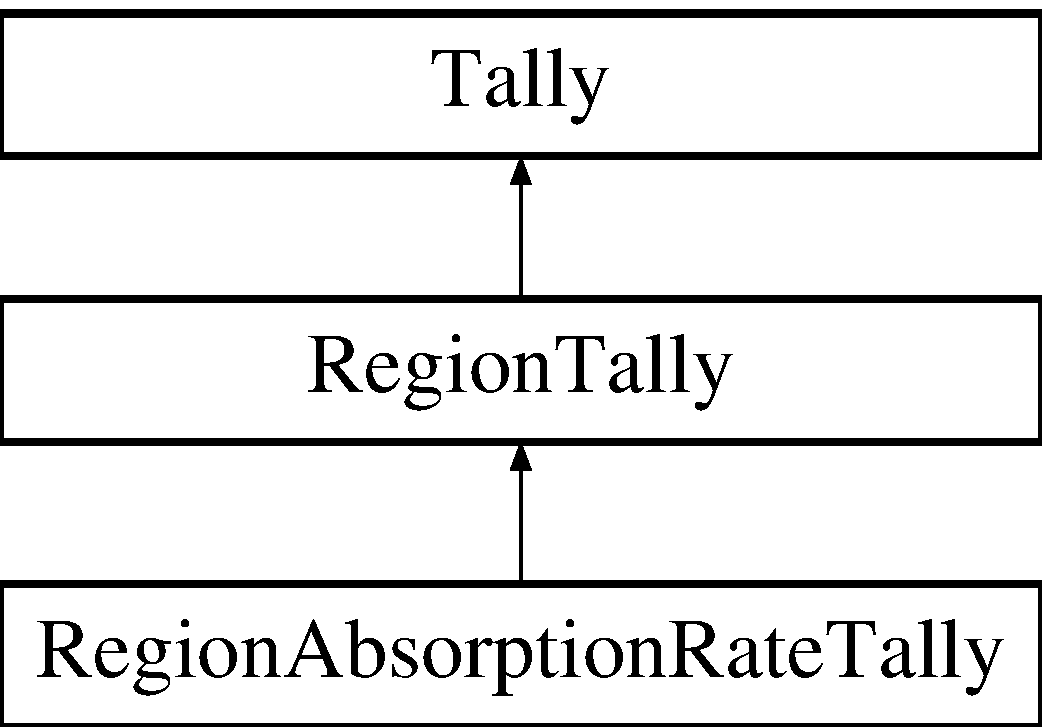
\includegraphics[height=3.000000cm]{classRegionAbsorptionRateTally}
\end{center}
\end{figure}
\subsection*{Public Member Functions}
\begin{DoxyCompactItemize}
\item 
\hyperlink{classRegionAbsorptionRateTally_a660ea8cbb625cad4ecb5a64e963a0682}{Region\-Absorption\-Rate\-Tally} (\hyperlink{classRegion}{Region} $\ast$region, const char $\ast$tally\-\_\-name=(char $\ast$)\char`\"{}\char`\"{})
\begin{DoxyCompactList}\small\item\em \hyperlink{classRegionAbsorptionRateTally}{Region\-Absorption\-Rate\-Tally} constructor calls the \hyperlink{classRegionTally}{Region\-Tally} constructor and \hyperlink{classTally}{Tally} constructors and sets the tally type to A\-B\-S\-O\-R\-P\-T\-I\-O\-N\-\_\-\-R\-A\-T\-E. \end{DoxyCompactList}\item 
void \hyperlink{classRegionAbsorptionRateTally_ac4b4c57159d65550e1e67dfb2037fd09}{tally} (\hyperlink{structneutron}{neutron} $\ast$\hyperlink{structneutron}{neutron})
\begin{DoxyCompactList}\small\item\em \hyperlink{classTally}{Tally} the region absorption rate by incrementing the tally by $ \frac{\Sigma_a}{\Sigma_t} $ at the neutron's energy. \end{DoxyCompactList}\end{DoxyCompactItemize}
\subsection*{Additional Inherited Members}


\subsection{Detailed Description}
A class for tallying the absorption rate within a region. 

\subsection{Constructor \& Destructor Documentation}
\hypertarget{classRegionAbsorptionRateTally_a660ea8cbb625cad4ecb5a64e963a0682}{\index{Region\-Absorption\-Rate\-Tally@{Region\-Absorption\-Rate\-Tally}!Region\-Absorption\-Rate\-Tally@{Region\-Absorption\-Rate\-Tally}}
\index{Region\-Absorption\-Rate\-Tally@{Region\-Absorption\-Rate\-Tally}!RegionAbsorptionRateTally@{Region\-Absorption\-Rate\-Tally}}
\subsubsection[{Region\-Absorption\-Rate\-Tally}]{\setlength{\rightskip}{0pt plus 5cm}Region\-Absorption\-Rate\-Tally\-::\-Region\-Absorption\-Rate\-Tally (
\begin{DoxyParamCaption}
\item[{{\bf Region} $\ast$}]{region, }
\item[{const char $\ast$}]{tally\-\_\-name = {\ttfamily (char$\ast$)\char`\"{}\char`\"{}}}
\end{DoxyParamCaption}
)\hspace{0.3cm}{\ttfamily [inline]}}}\label{classRegionAbsorptionRateTally_a660ea8cbb625cad4ecb5a64e963a0682}


\hyperlink{classRegionAbsorptionRateTally}{Region\-Absorption\-Rate\-Tally} constructor calls the \hyperlink{classRegionTally}{Region\-Tally} constructor and \hyperlink{classTally}{Tally} constructors and sets the tally type to A\-B\-S\-O\-R\-P\-T\-I\-O\-N\-\_\-\-R\-A\-T\-E. 


\begin{DoxyParams}{Parameters}
{\em region} & a pointer to the region within which to tally \\
\hline
{\em tally\-\_\-name} & a character array for the tally name (optional) \\
\hline
\end{DoxyParams}


\subsection{Member Function Documentation}
\hypertarget{classRegionAbsorptionRateTally_ac4b4c57159d65550e1e67dfb2037fd09}{\index{Region\-Absorption\-Rate\-Tally@{Region\-Absorption\-Rate\-Tally}!tally@{tally}}
\index{tally@{tally}!RegionAbsorptionRateTally@{Region\-Absorption\-Rate\-Tally}}
\subsubsection[{tally}]{\setlength{\rightskip}{0pt plus 5cm}void Region\-Absorption\-Rate\-Tally\-::tally (
\begin{DoxyParamCaption}
\item[{{\bf neutron} $\ast$}]{neutron}
\end{DoxyParamCaption}
)\hspace{0.3cm}{\ttfamily [virtual]}}}\label{classRegionAbsorptionRateTally_ac4b4c57159d65550e1e67dfb2037fd09}


\hyperlink{classTally}{Tally} the region absorption rate by incrementing the tally by $ \frac{\Sigma_a}{\Sigma_t} $ at the neutron's energy. 


\begin{DoxyParams}{Parameters}
{\em neutron} & the neutron of interest \\
\hline
\end{DoxyParams}


Implements \hyperlink{classRegionTally_ae146fd937e34306fdd5cc4aac44a3856}{Region\-Tally}.



The documentation for this class was generated from the following files\-:\begin{DoxyCompactItemize}
\item 
\hyperlink{Tally_8h}{Tally.\-h}\item 
Tally.\-cpp\end{DoxyCompactItemize}

\hypertarget{classRegionCaptureRateTally}{\section{Region\-Capture\-Rate\-Tally Class Reference}
\label{classRegionCaptureRateTally}\index{Region\-Capture\-Rate\-Tally@{Region\-Capture\-Rate\-Tally}}
}


A class for tallying the capture rate within a region.  




{\ttfamily \#include \char`\"{}pinspec/src/\-Tally.\-h\char`\"{}}

Inheritance diagram for Region\-Capture\-Rate\-Tally\-:\begin{figure}[H]
\begin{center}
\leavevmode
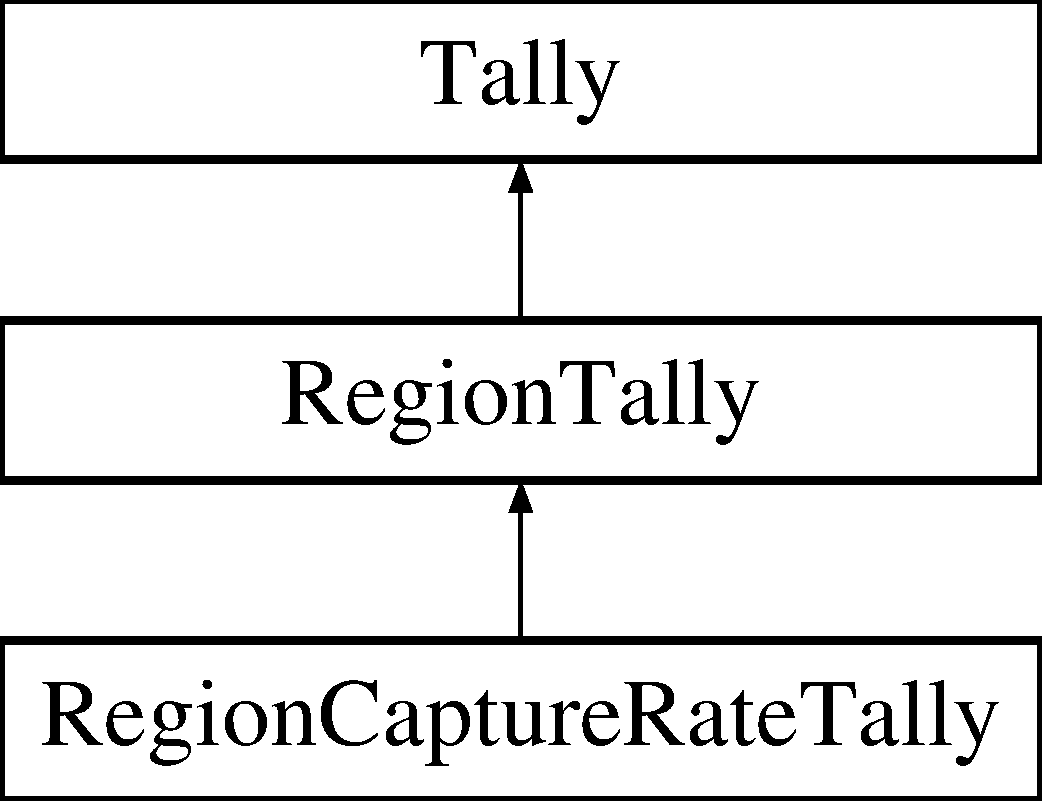
\includegraphics[height=3.000000cm]{classRegionCaptureRateTally}
\end{center}
\end{figure}
\subsection*{Public Member Functions}
\begin{DoxyCompactItemize}
\item 
\hyperlink{classRegionCaptureRateTally_a7d0e48235eb320f44fa11b4395e3b7ae}{Region\-Capture\-Rate\-Tally} (\hyperlink{classRegion}{Region} $\ast$region, const char $\ast$tally\-\_\-name=(char $\ast$)\char`\"{}\char`\"{})
\begin{DoxyCompactList}\small\item\em \hyperlink{classRegionCaptureRateTally}{Region\-Capture\-Rate\-Tally} constructor calls the \hyperlink{classRegionTally}{Region\-Tally} constructor and \hyperlink{classTally}{Tally} constructors and sets the tally type to C\-A\-P\-T\-U\-R\-E\-\_\-\-R\-A\-T\-E. \end{DoxyCompactList}\item 
void \hyperlink{classRegionCaptureRateTally_a200bb4afe0bdf5520cc9756f644ebcd3}{tally} (\hyperlink{structneutron}{neutron} $\ast$\hyperlink{structneutron}{neutron})
\begin{DoxyCompactList}\small\item\em \hyperlink{classTally}{Tally} the region capture rate by incrementing the tally by $ \frac{\Sigma_c}{\Sigma_t} $ at the neutron's energy. \end{DoxyCompactList}\end{DoxyCompactItemize}
\subsection*{Additional Inherited Members}


\subsection{Detailed Description}
A class for tallying the capture rate within a region. 

\subsection{Constructor \& Destructor Documentation}
\hypertarget{classRegionCaptureRateTally_a7d0e48235eb320f44fa11b4395e3b7ae}{\index{Region\-Capture\-Rate\-Tally@{Region\-Capture\-Rate\-Tally}!Region\-Capture\-Rate\-Tally@{Region\-Capture\-Rate\-Tally}}
\index{Region\-Capture\-Rate\-Tally@{Region\-Capture\-Rate\-Tally}!RegionCaptureRateTally@{Region\-Capture\-Rate\-Tally}}
\subsubsection[{Region\-Capture\-Rate\-Tally}]{\setlength{\rightskip}{0pt plus 5cm}Region\-Capture\-Rate\-Tally\-::\-Region\-Capture\-Rate\-Tally (
\begin{DoxyParamCaption}
\item[{{\bf Region} $\ast$}]{region, }
\item[{const char $\ast$}]{tally\-\_\-name = {\ttfamily (char$\ast$)\char`\"{}\char`\"{}}}
\end{DoxyParamCaption}
)\hspace{0.3cm}{\ttfamily [inline]}}}\label{classRegionCaptureRateTally_a7d0e48235eb320f44fa11b4395e3b7ae}


\hyperlink{classRegionCaptureRateTally}{Region\-Capture\-Rate\-Tally} constructor calls the \hyperlink{classRegionTally}{Region\-Tally} constructor and \hyperlink{classTally}{Tally} constructors and sets the tally type to C\-A\-P\-T\-U\-R\-E\-\_\-\-R\-A\-T\-E. 


\begin{DoxyParams}{Parameters}
{\em region} & a pointer to the region within which to tally \\
\hline
{\em tally\-\_\-name} & a character array for the tally name (optional) \\
\hline
\end{DoxyParams}


\subsection{Member Function Documentation}
\hypertarget{classRegionCaptureRateTally_a200bb4afe0bdf5520cc9756f644ebcd3}{\index{Region\-Capture\-Rate\-Tally@{Region\-Capture\-Rate\-Tally}!tally@{tally}}
\index{tally@{tally}!RegionCaptureRateTally@{Region\-Capture\-Rate\-Tally}}
\subsubsection[{tally}]{\setlength{\rightskip}{0pt plus 5cm}void Region\-Capture\-Rate\-Tally\-::tally (
\begin{DoxyParamCaption}
\item[{{\bf neutron} $\ast$}]{neutron}
\end{DoxyParamCaption}
)\hspace{0.3cm}{\ttfamily [virtual]}}}\label{classRegionCaptureRateTally_a200bb4afe0bdf5520cc9756f644ebcd3}


\hyperlink{classTally}{Tally} the region capture rate by incrementing the tally by $ \frac{\Sigma_c}{\Sigma_t} $ at the neutron's energy. 


\begin{DoxyParams}{Parameters}
{\em neutron} & the neutron of interest \\
\hline
\end{DoxyParams}


Implements \hyperlink{classRegionTally_ae146fd937e34306fdd5cc4aac44a3856}{Region\-Tally}.



The documentation for this class was generated from the following files\-:\begin{DoxyCompactItemize}
\item 
pinspec/src/\hyperlink{Tally_8h}{Tally.\-h}\item 
pinspec/src/Tally.\-cpp\end{DoxyCompactItemize}

\hypertarget{classRegionCollisionRateTally}{\section{Region\-Collision\-Rate\-Tally Class Reference}
\label{classRegionCollisionRateTally}\index{Region\-Collision\-Rate\-Tally@{Region\-Collision\-Rate\-Tally}}
}


A class for tallying the collision rate within a region.  




{\ttfamily \#include \char`\"{}pinspec/src/\-Tally.\-h\char`\"{}}

Inheritance diagram for Region\-Collision\-Rate\-Tally\-:\begin{figure}[H]
\begin{center}
\leavevmode
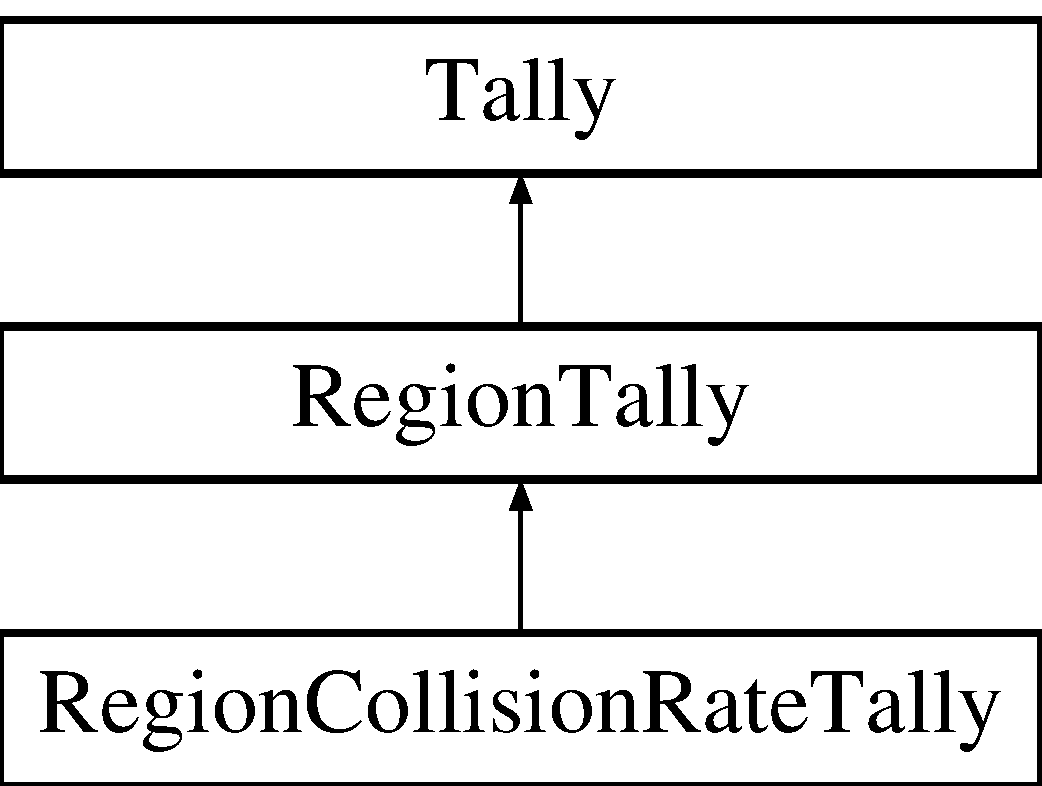
\includegraphics[height=3.000000cm]{classRegionCollisionRateTally}
\end{center}
\end{figure}
\subsection*{Public Member Functions}
\begin{DoxyCompactItemize}
\item 
\hyperlink{classRegionCollisionRateTally_a4665e117d3c7be7ce66ae9a23e031e73}{Region\-Collision\-Rate\-Tally} (\hyperlink{classRegion}{Region} $\ast$region, const char $\ast$tally\-\_\-name=(char $\ast$)\char`\"{}\char`\"{})
\begin{DoxyCompactList}\small\item\em \hyperlink{classRegionCollisionRateTally}{Region\-Collision\-Rate\-Tally} constructor calls the \hyperlink{classRegionTally}{Region\-Tally} constructor and \hyperlink{classTally}{Tally} constructors and sets the tally type to C\-O\-L\-L\-I\-S\-I\-O\-N\-\_\-\-R\-A\-T\-E. \end{DoxyCompactList}\item 
void \hyperlink{classRegionCollisionRateTally_af365f111715d80311047029fe2e64ce7}{tally} (\hyperlink{structneutron}{neutron} $\ast$\hyperlink{structneutron}{neutron})
\begin{DoxyCompactList}\small\item\em \hyperlink{classTally}{Tally} the region collision rate by incrementing the tally by 1.\-0 at the neutron's energy. \end{DoxyCompactList}\end{DoxyCompactItemize}
\subsection*{Additional Inherited Members}


\subsection{Detailed Description}
A class for tallying the collision rate within a region. 

\subsection{Constructor \& Destructor Documentation}
\hypertarget{classRegionCollisionRateTally_a4665e117d3c7be7ce66ae9a23e031e73}{\index{Region\-Collision\-Rate\-Tally@{Region\-Collision\-Rate\-Tally}!Region\-Collision\-Rate\-Tally@{Region\-Collision\-Rate\-Tally}}
\index{Region\-Collision\-Rate\-Tally@{Region\-Collision\-Rate\-Tally}!RegionCollisionRateTally@{Region\-Collision\-Rate\-Tally}}
\subsubsection[{Region\-Collision\-Rate\-Tally}]{\setlength{\rightskip}{0pt plus 5cm}Region\-Collision\-Rate\-Tally\-::\-Region\-Collision\-Rate\-Tally (
\begin{DoxyParamCaption}
\item[{{\bf Region} $\ast$}]{region, }
\item[{const char $\ast$}]{tally\-\_\-name = {\ttfamily (char$\ast$)\char`\"{}\char`\"{}}}
\end{DoxyParamCaption}
)\hspace{0.3cm}{\ttfamily [inline]}}}\label{classRegionCollisionRateTally_a4665e117d3c7be7ce66ae9a23e031e73}


\hyperlink{classRegionCollisionRateTally}{Region\-Collision\-Rate\-Tally} constructor calls the \hyperlink{classRegionTally}{Region\-Tally} constructor and \hyperlink{classTally}{Tally} constructors and sets the tally type to C\-O\-L\-L\-I\-S\-I\-O\-N\-\_\-\-R\-A\-T\-E. 


\begin{DoxyParams}{Parameters}
{\em region} & a pointer to the region within which to tally \\
\hline
{\em tally\-\_\-name} & a character array for the tally name (optional) \\
\hline
\end{DoxyParams}


\subsection{Member Function Documentation}
\hypertarget{classRegionCollisionRateTally_af365f111715d80311047029fe2e64ce7}{\index{Region\-Collision\-Rate\-Tally@{Region\-Collision\-Rate\-Tally}!tally@{tally}}
\index{tally@{tally}!RegionCollisionRateTally@{Region\-Collision\-Rate\-Tally}}
\subsubsection[{tally}]{\setlength{\rightskip}{0pt plus 5cm}void Region\-Collision\-Rate\-Tally\-::tally (
\begin{DoxyParamCaption}
\item[{{\bf neutron} $\ast$}]{neutron}
\end{DoxyParamCaption}
)\hspace{0.3cm}{\ttfamily [virtual]}}}\label{classRegionCollisionRateTally_af365f111715d80311047029fe2e64ce7}


\hyperlink{classTally}{Tally} the region collision rate by incrementing the tally by 1.\-0 at the neutron's energy. 


\begin{DoxyParams}{Parameters}
{\em neutron} & the neutron of interest \\
\hline
\end{DoxyParams}


Implements \hyperlink{classRegionTally_ae146fd937e34306fdd5cc4aac44a3856}{Region\-Tally}.



The documentation for this class was generated from the following files\-:\begin{DoxyCompactItemize}
\item 
pinspec/src/\hyperlink{Tally_8h}{Tally.\-h}\item 
pinspec/src/Tally.\-cpp\end{DoxyCompactItemize}

\hypertarget{classRegionDiffusionRateTally}{\section{Region\-Diffusion\-Rate\-Tally Class Reference}
\label{classRegionDiffusionRateTally}\index{Region\-Diffusion\-Rate\-Tally@{Region\-Diffusion\-Rate\-Tally}}
}


A class for tallying the diffusion rate within a region.  




{\ttfamily \#include \char`\"{}pinspec/src/\-Tally.\-h\char`\"{}}

Inheritance diagram for Region\-Diffusion\-Rate\-Tally\-:\begin{figure}[H]
\begin{center}
\leavevmode
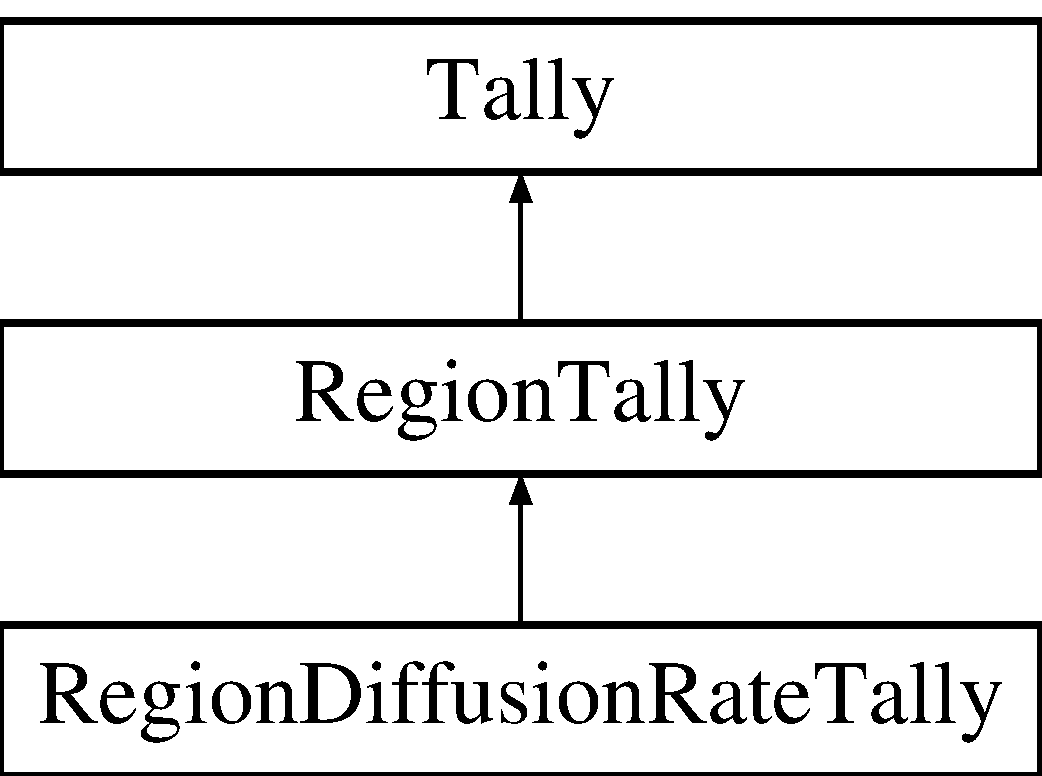
\includegraphics[height=3.000000cm]{classRegionDiffusionRateTally}
\end{center}
\end{figure}
\subsection*{Public Member Functions}
\begin{DoxyCompactItemize}
\item 
\hyperlink{classRegionDiffusionRateTally_a64dc61a22189a60f052cf349615d3463}{Region\-Diffusion\-Rate\-Tally} (\hyperlink{classRegion}{Region} $\ast$region, const char $\ast$tally\-\_\-name=(char $\ast$)\char`\"{}\char`\"{})
\begin{DoxyCompactList}\small\item\em \hyperlink{classRegionDiffusionRateTally}{Region\-Diffusion\-Rate\-Tally} constructor calls the \hyperlink{classRegionTally}{Region\-Tally} constructor and \hyperlink{classTally}{Tally} constructors and sets the tally type to D\-I\-F\-F\-U\-S\-I\-O\-N\-\_\-\-R\-A\-T\-E. \end{DoxyCompactList}\item 
void \hyperlink{classRegionDiffusionRateTally_a0c581304fc724c57632ed00b5f2e5e0f}{tally} (\hyperlink{structneutron}{neutron} $\ast$\hyperlink{structneutron}{neutron})
\begin{DoxyCompactList}\small\item\em \hyperlink{classTally}{Tally} the region diffusion rate by incrementing the tally by $ \frac{\frac{1}{3\Sigma_tr}}{\Sigma_t} $ at the neutron's energy. \end{DoxyCompactList}\end{DoxyCompactItemize}
\subsection*{Additional Inherited Members}


\subsection{Detailed Description}
A class for tallying the diffusion rate within a region. 

\subsection{Constructor \& Destructor Documentation}
\hypertarget{classRegionDiffusionRateTally_a64dc61a22189a60f052cf349615d3463}{\index{Region\-Diffusion\-Rate\-Tally@{Region\-Diffusion\-Rate\-Tally}!Region\-Diffusion\-Rate\-Tally@{Region\-Diffusion\-Rate\-Tally}}
\index{Region\-Diffusion\-Rate\-Tally@{Region\-Diffusion\-Rate\-Tally}!RegionDiffusionRateTally@{Region\-Diffusion\-Rate\-Tally}}
\subsubsection[{Region\-Diffusion\-Rate\-Tally}]{\setlength{\rightskip}{0pt plus 5cm}Region\-Diffusion\-Rate\-Tally\-::\-Region\-Diffusion\-Rate\-Tally (
\begin{DoxyParamCaption}
\item[{{\bf Region} $\ast$}]{region, }
\item[{const char $\ast$}]{tally\-\_\-name = {\ttfamily (char$\ast$)\char`\"{}\char`\"{}}}
\end{DoxyParamCaption}
)\hspace{0.3cm}{\ttfamily [inline]}}}\label{classRegionDiffusionRateTally_a64dc61a22189a60f052cf349615d3463}


\hyperlink{classRegionDiffusionRateTally}{Region\-Diffusion\-Rate\-Tally} constructor calls the \hyperlink{classRegionTally}{Region\-Tally} constructor and \hyperlink{classTally}{Tally} constructors and sets the tally type to D\-I\-F\-F\-U\-S\-I\-O\-N\-\_\-\-R\-A\-T\-E. 


\begin{DoxyParams}{Parameters}
{\em region} & a pointer to the region within which to tally \\
\hline
{\em tally\-\_\-name} & a character array for the tally name (optional) \\
\hline
\end{DoxyParams}


\subsection{Member Function Documentation}
\hypertarget{classRegionDiffusionRateTally_a0c581304fc724c57632ed00b5f2e5e0f}{\index{Region\-Diffusion\-Rate\-Tally@{Region\-Diffusion\-Rate\-Tally}!tally@{tally}}
\index{tally@{tally}!RegionDiffusionRateTally@{Region\-Diffusion\-Rate\-Tally}}
\subsubsection[{tally}]{\setlength{\rightskip}{0pt plus 5cm}void Region\-Diffusion\-Rate\-Tally\-::tally (
\begin{DoxyParamCaption}
\item[{{\bf neutron} $\ast$}]{neutron}
\end{DoxyParamCaption}
)\hspace{0.3cm}{\ttfamily [virtual]}}}\label{classRegionDiffusionRateTally_a0c581304fc724c57632ed00b5f2e5e0f}


\hyperlink{classTally}{Tally} the region diffusion rate by incrementing the tally by $ \frac{\frac{1}{3\Sigma_tr}}{\Sigma_t} $ at the neutron's energy. 


\begin{DoxyParams}{Parameters}
{\em neutron} & the neutron of interest \\
\hline
\end{DoxyParams}


Implements \hyperlink{classRegionTally_ae146fd937e34306fdd5cc4aac44a3856}{Region\-Tally}.



The documentation for this class was generated from the following files\-:\begin{DoxyCompactItemize}
\item 
\hyperlink{Tally_8h}{Tally.\-h}\item 
Tally.\-cpp\end{DoxyCompactItemize}

\hypertarget{classRegionElasticRateTally}{\section{Region\-Elastic\-Rate\-Tally Class Reference}
\label{classRegionElasticRateTally}\index{Region\-Elastic\-Rate\-Tally@{Region\-Elastic\-Rate\-Tally}}
}


A class for tallying the elastic scattering rate within a region.  




{\ttfamily \#include \char`\"{}pinspec/src/\-Tally.\-h\char`\"{}}

Inheritance diagram for Region\-Elastic\-Rate\-Tally\-:\begin{figure}[H]
\begin{center}
\leavevmode
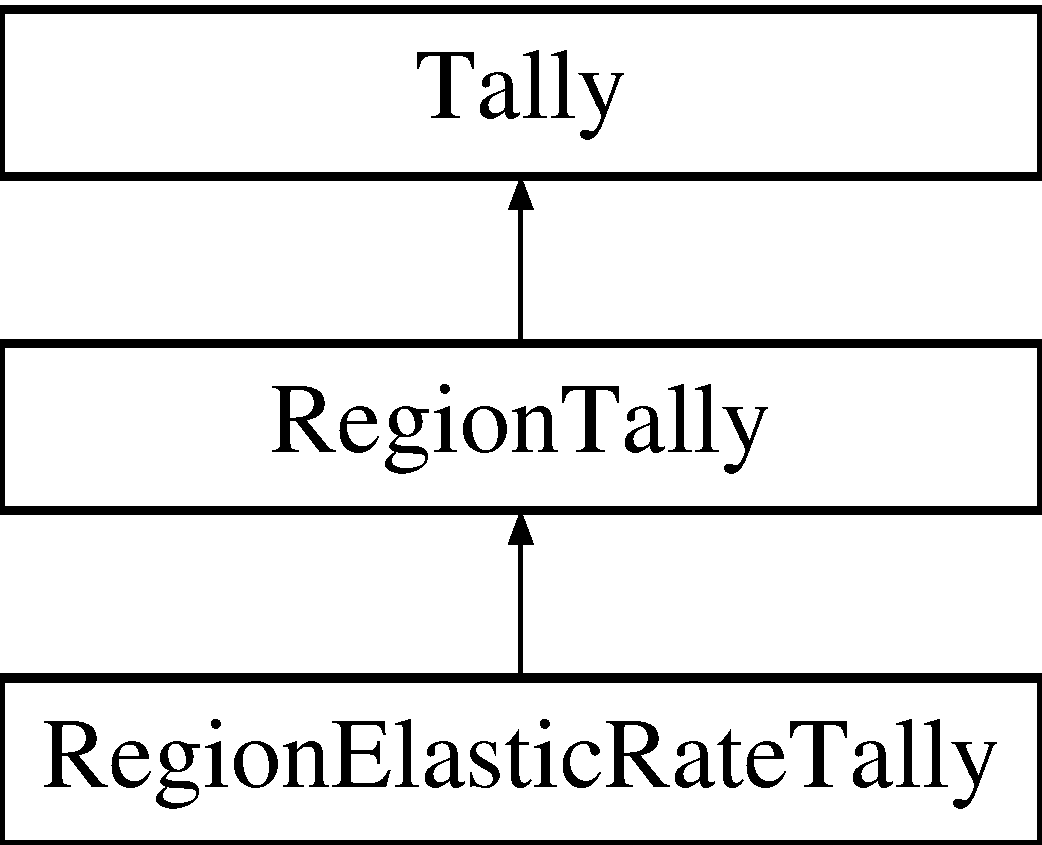
\includegraphics[height=3.000000cm]{classRegionElasticRateTally}
\end{center}
\end{figure}
\subsection*{Public Member Functions}
\begin{DoxyCompactItemize}
\item 
\hyperlink{classRegionElasticRateTally_aab82cda6914a01240b7fdfe01ca08b33}{Region\-Elastic\-Rate\-Tally} (\hyperlink{classRegion}{Region} $\ast$region, const char $\ast$tally\-\_\-name=(char $\ast$)\char`\"{}\char`\"{})
\begin{DoxyCompactList}\small\item\em \hyperlink{classRegionElasticRateTally}{Region\-Elastic\-Rate\-Tally} constructor calls the \hyperlink{classRegionTally}{Region\-Tally} constructor and \hyperlink{classTally}{Tally} constructors and sets the tally type to E\-L\-A\-S\-T\-I\-C\-\_\-\-R\-A\-T\-E. \end{DoxyCompactList}\item 
void \hyperlink{classRegionElasticRateTally_aaafa18c6ed2d9d2da1437cb1d969fa29}{tally} (\hyperlink{structneutron}{neutron} $\ast$\hyperlink{structneutron}{neutron})
\begin{DoxyCompactList}\small\item\em \hyperlink{classTally}{Tally} the material elastic scattering rate by incrementing the tally by $ \frac{\Sigma_s}{\Sigma_t} $ at the neutron's energy. \end{DoxyCompactList}\end{DoxyCompactItemize}
\subsection*{Additional Inherited Members}


\subsection{Detailed Description}
A class for tallying the elastic scattering rate within a region. 

\subsection{Constructor \& Destructor Documentation}
\hypertarget{classRegionElasticRateTally_aab82cda6914a01240b7fdfe01ca08b33}{\index{Region\-Elastic\-Rate\-Tally@{Region\-Elastic\-Rate\-Tally}!Region\-Elastic\-Rate\-Tally@{Region\-Elastic\-Rate\-Tally}}
\index{Region\-Elastic\-Rate\-Tally@{Region\-Elastic\-Rate\-Tally}!RegionElasticRateTally@{Region\-Elastic\-Rate\-Tally}}
\subsubsection[{Region\-Elastic\-Rate\-Tally}]{\setlength{\rightskip}{0pt plus 5cm}Region\-Elastic\-Rate\-Tally\-::\-Region\-Elastic\-Rate\-Tally (
\begin{DoxyParamCaption}
\item[{{\bf Region} $\ast$}]{region, }
\item[{const char $\ast$}]{tally\-\_\-name = {\ttfamily (char$\ast$)\char`\"{}\char`\"{}}}
\end{DoxyParamCaption}
)\hspace{0.3cm}{\ttfamily [inline]}}}\label{classRegionElasticRateTally_aab82cda6914a01240b7fdfe01ca08b33}


\hyperlink{classRegionElasticRateTally}{Region\-Elastic\-Rate\-Tally} constructor calls the \hyperlink{classRegionTally}{Region\-Tally} constructor and \hyperlink{classTally}{Tally} constructors and sets the tally type to E\-L\-A\-S\-T\-I\-C\-\_\-\-R\-A\-T\-E. 


\begin{DoxyParams}{Parameters}
{\em region} & a pointer to the region within which to tally \\
\hline
{\em tally\-\_\-name} & a character array for the tally name (optional) \\
\hline
\end{DoxyParams}


\subsection{Member Function Documentation}
\hypertarget{classRegionElasticRateTally_aaafa18c6ed2d9d2da1437cb1d969fa29}{\index{Region\-Elastic\-Rate\-Tally@{Region\-Elastic\-Rate\-Tally}!tally@{tally}}
\index{tally@{tally}!RegionElasticRateTally@{Region\-Elastic\-Rate\-Tally}}
\subsubsection[{tally}]{\setlength{\rightskip}{0pt plus 5cm}void Region\-Elastic\-Rate\-Tally\-::tally (
\begin{DoxyParamCaption}
\item[{{\bf neutron} $\ast$}]{neutron}
\end{DoxyParamCaption}
)\hspace{0.3cm}{\ttfamily [virtual]}}}\label{classRegionElasticRateTally_aaafa18c6ed2d9d2da1437cb1d969fa29}


\hyperlink{classTally}{Tally} the material elastic scattering rate by incrementing the tally by $ \frac{\Sigma_s}{\Sigma_t} $ at the neutron's energy. 


\begin{DoxyParams}{Parameters}
{\em neutron} & the neutron of interest \\
\hline
\end{DoxyParams}


Implements \hyperlink{classRegionTally_ae146fd937e34306fdd5cc4aac44a3856}{Region\-Tally}.



The documentation for this class was generated from the following files\-:\begin{DoxyCompactItemize}
\item 
pinspec/src/\hyperlink{Tally_8h}{Tally.\-h}\item 
pinspec/src/Tally.\-cpp\end{DoxyCompactItemize}

\hypertarget{classRegionFissionRateTally}{\section{Region\-Fission\-Rate\-Tally Class Reference}
\label{classRegionFissionRateTally}\index{Region\-Fission\-Rate\-Tally@{Region\-Fission\-Rate\-Tally}}
}


A class for tallying the fission rate within a region..  




{\ttfamily \#include \char`\"{}pinspec/src/\-Tally.\-h\char`\"{}}

Inheritance diagram for Region\-Fission\-Rate\-Tally\-:\begin{figure}[H]
\begin{center}
\leavevmode
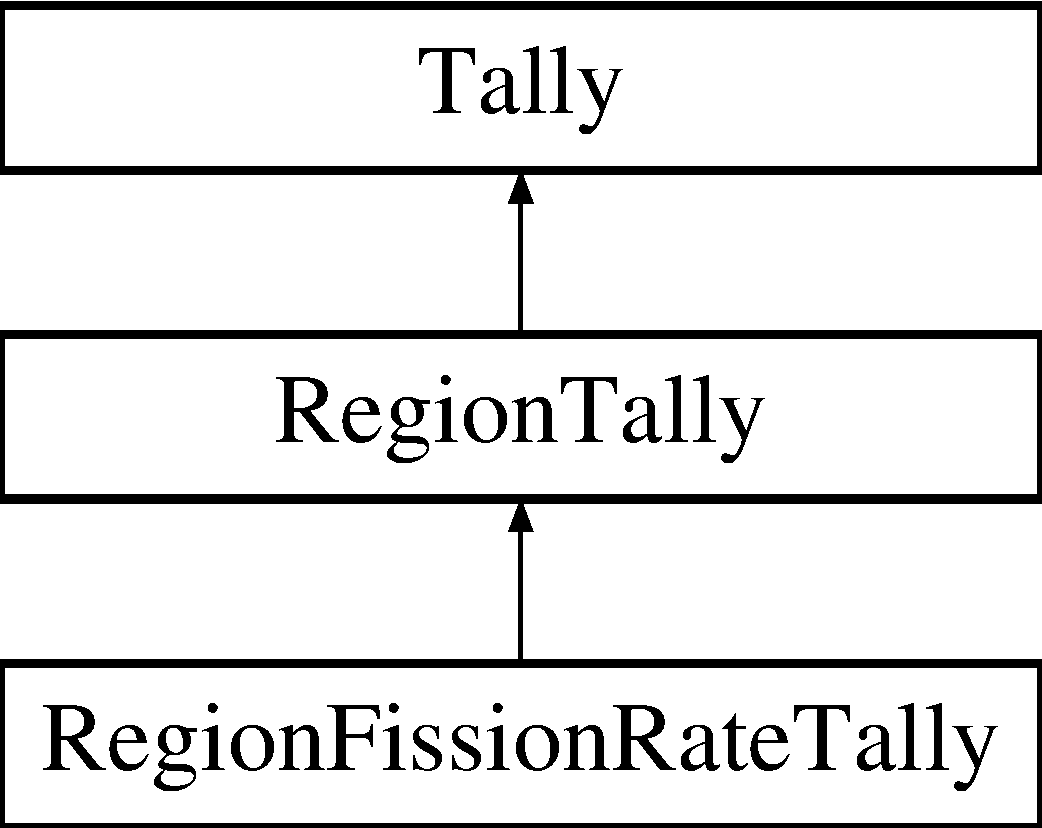
\includegraphics[height=3.000000cm]{classRegionFissionRateTally}
\end{center}
\end{figure}
\subsection*{Public Member Functions}
\begin{DoxyCompactItemize}
\item 
\hyperlink{classRegionFissionRateTally_af3344001e9ba2ac13119191e49111d3d}{Region\-Fission\-Rate\-Tally} (\hyperlink{classRegion}{Region} $\ast$region, const char $\ast$tally\-\_\-name=(char $\ast$)\char`\"{}\char`\"{})
\begin{DoxyCompactList}\small\item\em \hyperlink{classRegionFissionRateTally}{Region\-Fission\-Rate\-Tally} constructor calls the \hyperlink{classRegionTally}{Region\-Tally} constructor and \hyperlink{classTally}{Tally} constructors and sets the tally type to F\-I\-S\-S\-I\-O\-N\-\_\-\-R\-A\-T\-E. \end{DoxyCompactList}\item 
void \hyperlink{classRegionFissionRateTally_a1d6e8da254f83a462de8ccf5226f1fee}{tally} (\hyperlink{structneutron}{neutron} $\ast$\hyperlink{structneutron}{neutron})
\begin{DoxyCompactList}\small\item\em \hyperlink{classTally}{Tally} the region fission rate by incrementing the tally by $ \frac{\Sigma_f}{\Sigma_t} $ at the neutron's energy. \end{DoxyCompactList}\end{DoxyCompactItemize}
\subsection*{Additional Inherited Members}


\subsection{Detailed Description}
A class for tallying the fission rate within a region.. 

\subsection{Constructor \& Destructor Documentation}
\hypertarget{classRegionFissionRateTally_af3344001e9ba2ac13119191e49111d3d}{\index{Region\-Fission\-Rate\-Tally@{Region\-Fission\-Rate\-Tally}!Region\-Fission\-Rate\-Tally@{Region\-Fission\-Rate\-Tally}}
\index{Region\-Fission\-Rate\-Tally@{Region\-Fission\-Rate\-Tally}!RegionFissionRateTally@{Region\-Fission\-Rate\-Tally}}
\subsubsection[{Region\-Fission\-Rate\-Tally}]{\setlength{\rightskip}{0pt plus 5cm}Region\-Fission\-Rate\-Tally\-::\-Region\-Fission\-Rate\-Tally (
\begin{DoxyParamCaption}
\item[{{\bf Region} $\ast$}]{region, }
\item[{const char $\ast$}]{tally\-\_\-name = {\ttfamily (char$\ast$)\char`\"{}\char`\"{}}}
\end{DoxyParamCaption}
)\hspace{0.3cm}{\ttfamily [inline]}}}\label{classRegionFissionRateTally_af3344001e9ba2ac13119191e49111d3d}


\hyperlink{classRegionFissionRateTally}{Region\-Fission\-Rate\-Tally} constructor calls the \hyperlink{classRegionTally}{Region\-Tally} constructor and \hyperlink{classTally}{Tally} constructors and sets the tally type to F\-I\-S\-S\-I\-O\-N\-\_\-\-R\-A\-T\-E. 


\begin{DoxyParams}{Parameters}
{\em region} & a pointer to the region within which to tally \\
\hline
{\em tally\-\_\-name} & a character array for the tally name (optional) \\
\hline
\end{DoxyParams}


\subsection{Member Function Documentation}
\hypertarget{classRegionFissionRateTally_a1d6e8da254f83a462de8ccf5226f1fee}{\index{Region\-Fission\-Rate\-Tally@{Region\-Fission\-Rate\-Tally}!tally@{tally}}
\index{tally@{tally}!RegionFissionRateTally@{Region\-Fission\-Rate\-Tally}}
\subsubsection[{tally}]{\setlength{\rightskip}{0pt plus 5cm}void Region\-Fission\-Rate\-Tally\-::tally (
\begin{DoxyParamCaption}
\item[{{\bf neutron} $\ast$}]{neutron}
\end{DoxyParamCaption}
)\hspace{0.3cm}{\ttfamily [virtual]}}}\label{classRegionFissionRateTally_a1d6e8da254f83a462de8ccf5226f1fee}


\hyperlink{classTally}{Tally} the region fission rate by incrementing the tally by $ \frac{\Sigma_f}{\Sigma_t} $ at the neutron's energy. 


\begin{DoxyParams}{Parameters}
{\em neutron} & the neutron of interest \\
\hline
\end{DoxyParams}


Implements \hyperlink{classRegionTally_ae146fd937e34306fdd5cc4aac44a3856}{Region\-Tally}.



The documentation for this class was generated from the following files\-:\begin{DoxyCompactItemize}
\item 
\hyperlink{Tally_8h}{Tally.\-h}\item 
Tally.\-cpp\end{DoxyCompactItemize}

\hypertarget{classRegionFluxTally}{\section{Region\-Flux\-Tally Class Reference}
\label{classRegionFluxTally}\index{Region\-Flux\-Tally@{Region\-Flux\-Tally}}
}


A class for tallying the flux for a region.  




{\ttfamily \#include \char`\"{}pinspec/src/\-Tally.\-h\char`\"{}}

Inheritance diagram for Region\-Flux\-Tally\-:\begin{figure}[H]
\begin{center}
\leavevmode
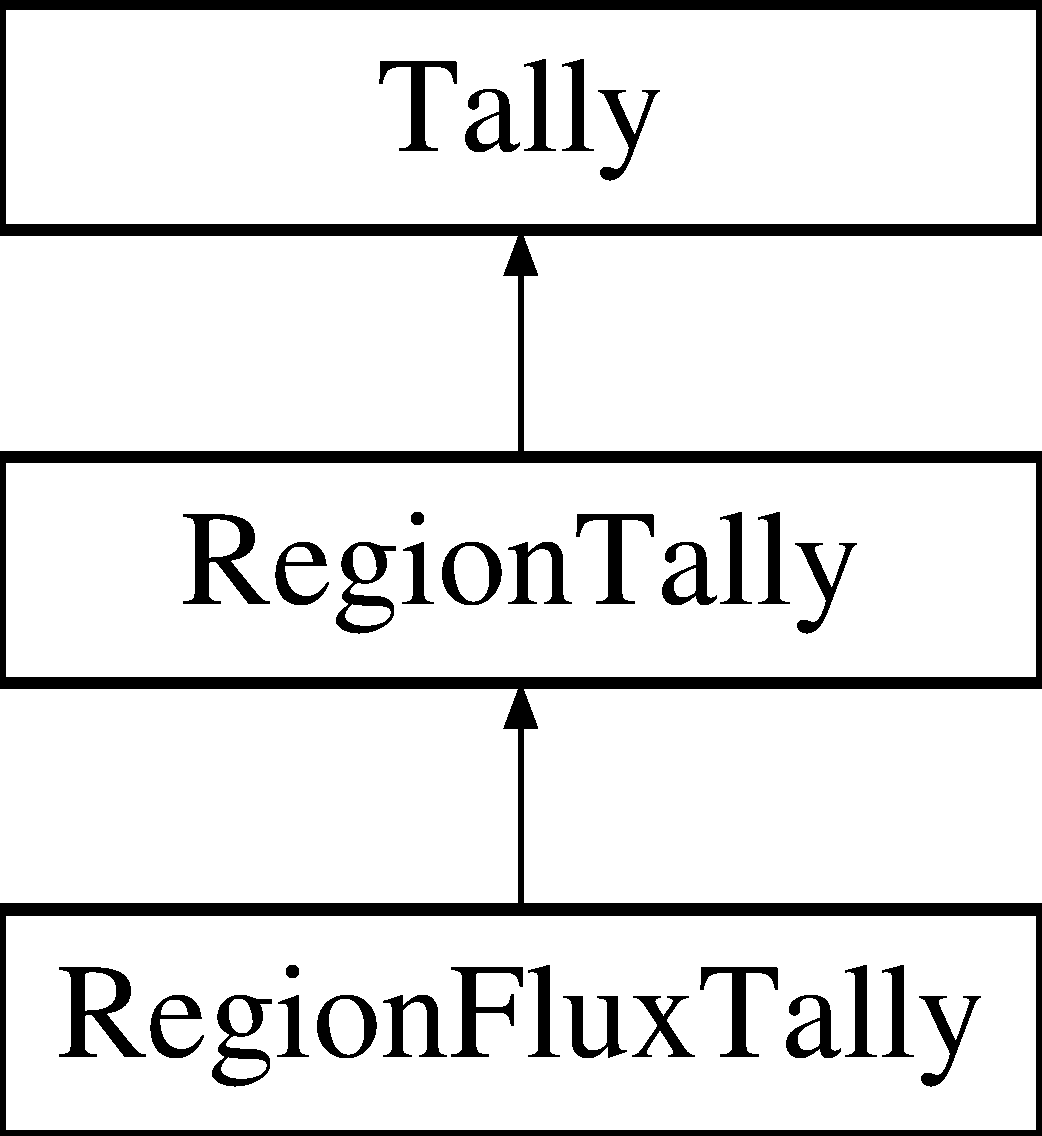
\includegraphics[height=3.000000cm]{classRegionFluxTally}
\end{center}
\end{figure}
\subsection*{Public Member Functions}
\begin{DoxyCompactItemize}
\item 
\hyperlink{classRegionFluxTally_afeb527c4b8deafc6cff68594ad95a9c8}{Region\-Flux\-Tally} (\hyperlink{classRegion}{Region} $\ast$region, const char $\ast$tally\-\_\-name=(char $\ast$)\char`\"{}\char`\"{})
\begin{DoxyCompactList}\small\item\em \hyperlink{classRegionFluxTally}{Region\-Flux\-Tally} constructor calls the \hyperlink{classRegionTally}{Region\-Tally} constructor and \hyperlink{classTally}{Tally} constructors and sets the tally type to F\-L\-U\-X. \end{DoxyCompactList}\item 
void \hyperlink{classRegionFluxTally_a318a32edcb4f2866574194cd74ddd04f}{tally} (\hyperlink{structneutron}{neutron} $\ast$\hyperlink{structneutron}{neutron})
\begin{DoxyCompactList}\small\item\em \hyperlink{classTally}{Tally} the region flux by incrementing the tally by $ \frac{1}{\Sigma_t} $ at the neutron's energy. \end{DoxyCompactList}\end{DoxyCompactItemize}
\subsection*{Additional Inherited Members}


\subsection{Detailed Description}
A class for tallying the flux for a region. 

\subsection{Constructor \& Destructor Documentation}
\hypertarget{classRegionFluxTally_afeb527c4b8deafc6cff68594ad95a9c8}{\index{Region\-Flux\-Tally@{Region\-Flux\-Tally}!Region\-Flux\-Tally@{Region\-Flux\-Tally}}
\index{Region\-Flux\-Tally@{Region\-Flux\-Tally}!RegionFluxTally@{Region\-Flux\-Tally}}
\subsubsection[{Region\-Flux\-Tally}]{\setlength{\rightskip}{0pt plus 5cm}Region\-Flux\-Tally\-::\-Region\-Flux\-Tally (
\begin{DoxyParamCaption}
\item[{{\bf Region} $\ast$}]{region, }
\item[{const char $\ast$}]{tally\-\_\-name = {\ttfamily (char$\ast$)\char`\"{}\char`\"{}}}
\end{DoxyParamCaption}
)\hspace{0.3cm}{\ttfamily [inline]}}}\label{classRegionFluxTally_afeb527c4b8deafc6cff68594ad95a9c8}


\hyperlink{classRegionFluxTally}{Region\-Flux\-Tally} constructor calls the \hyperlink{classRegionTally}{Region\-Tally} constructor and \hyperlink{classTally}{Tally} constructors and sets the tally type to F\-L\-U\-X. 


\begin{DoxyParams}{Parameters}
{\em region} & a pointer to the region within which to tally \\
\hline
{\em tally\-\_\-name} & a character array for the tally name (optional) \\
\hline
\end{DoxyParams}


\subsection{Member Function Documentation}
\hypertarget{classRegionFluxTally_a318a32edcb4f2866574194cd74ddd04f}{\index{Region\-Flux\-Tally@{Region\-Flux\-Tally}!tally@{tally}}
\index{tally@{tally}!RegionFluxTally@{Region\-Flux\-Tally}}
\subsubsection[{tally}]{\setlength{\rightskip}{0pt plus 5cm}void Region\-Flux\-Tally\-::tally (
\begin{DoxyParamCaption}
\item[{{\bf neutron} $\ast$}]{neutron}
\end{DoxyParamCaption}
)\hspace{0.3cm}{\ttfamily [virtual]}}}\label{classRegionFluxTally_a318a32edcb4f2866574194cd74ddd04f}


\hyperlink{classTally}{Tally} the region flux by incrementing the tally by $ \frac{1}{\Sigma_t} $ at the neutron's energy. 


\begin{DoxyParams}{Parameters}
{\em neutron} & the neutron of interest \\
\hline
\end{DoxyParams}


Implements \hyperlink{classRegionTally_ae146fd937e34306fdd5cc4aac44a3856}{Region\-Tally}.



The documentation for this class was generated from the following files\-:\begin{DoxyCompactItemize}
\item 
\hyperlink{Tally_8h}{Tally.\-h}\item 
Tally.\-cpp\end{DoxyCompactItemize}

\hypertarget{classRegionInterCollisionTimeTally}{\section{Region\-Inter\-Collision\-Time\-Tally Class Reference}
\label{classRegionInterCollisionTimeTally}\index{Region\-Inter\-Collision\-Time\-Tally@{Region\-Inter\-Collision\-Time\-Tally}}
}


A class for tallying the time between collisions for the region.  




{\ttfamily \#include \char`\"{}pinspec/src/\-Tally.\-h\char`\"{}}

Inheritance diagram for Region\-Inter\-Collision\-Time\-Tally\-:\begin{figure}[H]
\begin{center}
\leavevmode
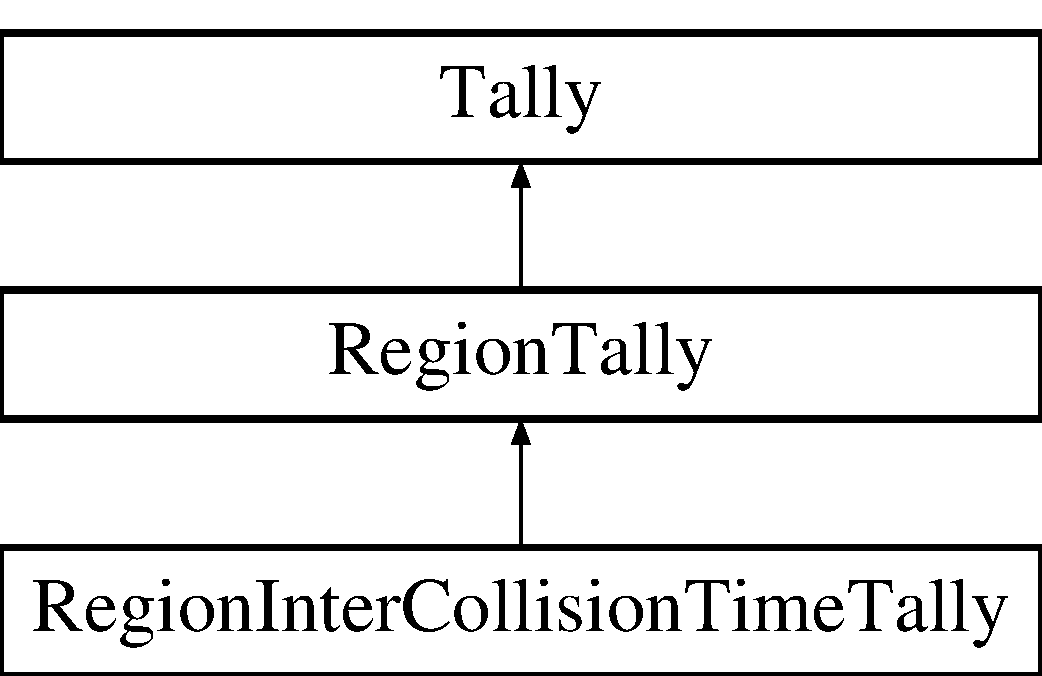
\includegraphics[height=3.000000cm]{classRegionInterCollisionTimeTally}
\end{center}
\end{figure}
\subsection*{Public Member Functions}
\begin{DoxyCompactItemize}
\item 
\hyperlink{classRegionInterCollisionTimeTally_ac80f657141e0c7388092e41f25e228f1}{Region\-Inter\-Collision\-Time\-Tally} (\hyperlink{classRegion}{Region} $\ast$region, const char $\ast$tally\-\_\-name=(char $\ast$)\char`\"{}\char`\"{})
\begin{DoxyCompactList}\small\item\em \hyperlink{classRegionInterCollisionTimeTally}{Region\-Inter\-Collision\-Time\-Tally} constructor calls the \hyperlink{classRegionTally}{Region\-Tally} constructor and \hyperlink{classTally}{Tally} constructors and sets the tally type to I\-N\-T\-E\-R\-C\-O\-L\-L\-I\-S\-I\-O\-N\-\_\-\-T\-I\-M\-E. \end{DoxyCompactList}\item 
void \hyperlink{classRegionInterCollisionTimeTally_a389dd158a3a10b959fa444d12a8cb752}{tally} (\hyperlink{structneutron}{neutron} $\ast$\hyperlink{structneutron}{neutron})
\begin{DoxyCompactList}\small\item\em \hyperlink{classTally}{Tally} the time between collisions by incrementing the tally with the travel time spent by this neutron to reach this collision\-: \end{DoxyCompactList}\end{DoxyCompactItemize}
\subsection*{Additional Inherited Members}


\subsection{Detailed Description}
A class for tallying the time between collisions for the region. 

\subsection{Constructor \& Destructor Documentation}
\hypertarget{classRegionInterCollisionTimeTally_ac80f657141e0c7388092e41f25e228f1}{\index{Region\-Inter\-Collision\-Time\-Tally@{Region\-Inter\-Collision\-Time\-Tally}!Region\-Inter\-Collision\-Time\-Tally@{Region\-Inter\-Collision\-Time\-Tally}}
\index{Region\-Inter\-Collision\-Time\-Tally@{Region\-Inter\-Collision\-Time\-Tally}!RegionInterCollisionTimeTally@{Region\-Inter\-Collision\-Time\-Tally}}
\subsubsection[{Region\-Inter\-Collision\-Time\-Tally}]{\setlength{\rightskip}{0pt plus 5cm}Region\-Inter\-Collision\-Time\-Tally\-::\-Region\-Inter\-Collision\-Time\-Tally (
\begin{DoxyParamCaption}
\item[{{\bf Region} $\ast$}]{region, }
\item[{const char $\ast$}]{tally\-\_\-name = {\ttfamily (char$\ast$)\char`\"{}\char`\"{}}}
\end{DoxyParamCaption}
)\hspace{0.3cm}{\ttfamily [inline]}}}\label{classRegionInterCollisionTimeTally_ac80f657141e0c7388092e41f25e228f1}


\hyperlink{classRegionInterCollisionTimeTally}{Region\-Inter\-Collision\-Time\-Tally} constructor calls the \hyperlink{classRegionTally}{Region\-Tally} constructor and \hyperlink{classTally}{Tally} constructors and sets the tally type to I\-N\-T\-E\-R\-C\-O\-L\-L\-I\-S\-I\-O\-N\-\_\-\-T\-I\-M\-E. 


\begin{DoxyParams}{Parameters}
{\em region} & a pointer to the region within which to tally \\
\hline
{\em tally\-\_\-name} & a character array for the tally name (optional) \\
\hline
\end{DoxyParams}


\subsection{Member Function Documentation}
\hypertarget{classRegionInterCollisionTimeTally_a389dd158a3a10b959fa444d12a8cb752}{\index{Region\-Inter\-Collision\-Time\-Tally@{Region\-Inter\-Collision\-Time\-Tally}!tally@{tally}}
\index{tally@{tally}!RegionInterCollisionTimeTally@{Region\-Inter\-Collision\-Time\-Tally}}
\subsubsection[{tally}]{\setlength{\rightskip}{0pt plus 5cm}void Region\-Inter\-Collision\-Time\-Tally\-::tally (
\begin{DoxyParamCaption}
\item[{{\bf neutron} $\ast$}]{neutron}
\end{DoxyParamCaption}
)\hspace{0.3cm}{\ttfamily [virtual]}}}\label{classRegionInterCollisionTimeTally_a389dd158a3a10b959fa444d12a8cb752}


\hyperlink{classTally}{Tally} the time between collisions by incrementing the tally with the travel time spent by this neutron to reach this collision\-: 

$ d = \frac{1}{\Sigma_t} $ $ v = c\sqrt{2Em_n} $ $ time = \frac{d}{v} $ 
\begin{DoxyParams}{Parameters}
{\em neutron} & the neutron of interest \\
\hline
\end{DoxyParams}


Implements \hyperlink{classRegionTally_ae146fd937e34306fdd5cc4aac44a3856}{Region\-Tally}.



The documentation for this class was generated from the following files\-:\begin{DoxyCompactItemize}
\item 
\hyperlink{Tally_8h}{Tally.\-h}\item 
Tally.\-cpp\end{DoxyCompactItemize}

\hypertarget{classRegionLeakageRateTally}{\section{Region\-Leakage\-Rate\-Tally Class Reference}
\label{classRegionLeakageRateTally}\index{Region\-Leakage\-Rate\-Tally@{Region\-Leakage\-Rate\-Tally}}
}


A class for tallying the leakage rate for a region.  




{\ttfamily \#include \char`\"{}pinspec/src/\-Tally.\-h\char`\"{}}

Inheritance diagram for Region\-Leakage\-Rate\-Tally\-:\begin{figure}[H]
\begin{center}
\leavevmode
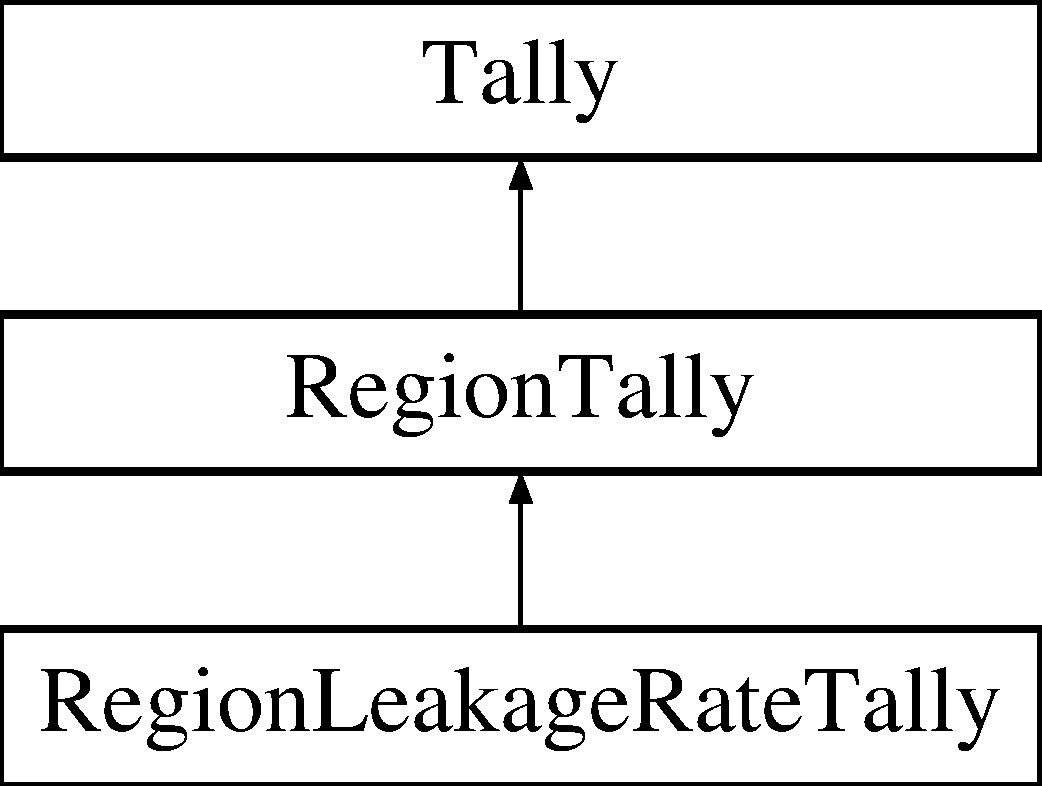
\includegraphics[height=3.000000cm]{classRegionLeakageRateTally}
\end{center}
\end{figure}
\subsection*{Public Member Functions}
\begin{DoxyCompactItemize}
\item 
\hyperlink{classRegionLeakageRateTally_a273616ced1ebb70364c29da24669793c}{Region\-Leakage\-Rate\-Tally} (\hyperlink{classRegion}{Region} $\ast$region, const char $\ast$tally\-\_\-name=(char $\ast$)\char`\"{}\char`\"{})
\begin{DoxyCompactList}\small\item\em \hyperlink{classRegionLeakageRateTally}{Region\-Leakage\-Rate\-Tally} constructor calls the \hyperlink{classRegionTally}{Region\-Tally} constructor and \hyperlink{classTally}{Tally} constructors and sets the tally type to L\-E\-A\-K\-A\-G\-E\-\_\-\-R\-A\-T\-E. \end{DoxyCompactList}\item 
void \hyperlink{classRegionLeakageRateTally_a9f8749a387783d68de8fc8ecaf347748}{tally} (\hyperlink{structneutron}{neutron} $\ast$\hyperlink{structneutron}{neutron})
\begin{DoxyCompactList}\small\item\em \hyperlink{classTally}{Tally} the region leakage rate by incrementing the tally by $ DB^2 $ at the neutron's energy. \end{DoxyCompactList}\end{DoxyCompactItemize}
\subsection*{Additional Inherited Members}


\subsection{Detailed Description}
A class for tallying the leakage rate for a region. 

\subsection{Constructor \& Destructor Documentation}
\hypertarget{classRegionLeakageRateTally_a273616ced1ebb70364c29da24669793c}{\index{Region\-Leakage\-Rate\-Tally@{Region\-Leakage\-Rate\-Tally}!Region\-Leakage\-Rate\-Tally@{Region\-Leakage\-Rate\-Tally}}
\index{Region\-Leakage\-Rate\-Tally@{Region\-Leakage\-Rate\-Tally}!RegionLeakageRateTally@{Region\-Leakage\-Rate\-Tally}}
\subsubsection[{Region\-Leakage\-Rate\-Tally}]{\setlength{\rightskip}{0pt plus 5cm}Region\-Leakage\-Rate\-Tally\-::\-Region\-Leakage\-Rate\-Tally (
\begin{DoxyParamCaption}
\item[{{\bf Region} $\ast$}]{region, }
\item[{const char $\ast$}]{tally\-\_\-name = {\ttfamily (char$\ast$)\char`\"{}\char`\"{}}}
\end{DoxyParamCaption}
)\hspace{0.3cm}{\ttfamily [inline]}}}\label{classRegionLeakageRateTally_a273616ced1ebb70364c29da24669793c}


\hyperlink{classRegionLeakageRateTally}{Region\-Leakage\-Rate\-Tally} constructor calls the \hyperlink{classRegionTally}{Region\-Tally} constructor and \hyperlink{classTally}{Tally} constructors and sets the tally type to L\-E\-A\-K\-A\-G\-E\-\_\-\-R\-A\-T\-E. 


\begin{DoxyParams}{Parameters}
{\em region} & a pointer to the region within which to tally \\
\hline
{\em tally\-\_\-name} & a character array for the tally name (optional) \\
\hline
\end{DoxyParams}


\subsection{Member Function Documentation}
\hypertarget{classRegionLeakageRateTally_a9f8749a387783d68de8fc8ecaf347748}{\index{Region\-Leakage\-Rate\-Tally@{Region\-Leakage\-Rate\-Tally}!tally@{tally}}
\index{tally@{tally}!RegionLeakageRateTally@{Region\-Leakage\-Rate\-Tally}}
\subsubsection[{tally}]{\setlength{\rightskip}{0pt plus 5cm}void Region\-Leakage\-Rate\-Tally\-::tally (
\begin{DoxyParamCaption}
\item[{{\bf neutron} $\ast$}]{neutron}
\end{DoxyParamCaption}
)\hspace{0.3cm}{\ttfamily [virtual]}}}\label{classRegionLeakageRateTally_a9f8749a387783d68de8fc8ecaf347748}


\hyperlink{classTally}{Tally} the region leakage rate by incrementing the tally by $ DB^2 $ at the neutron's energy. 


\begin{DoxyParams}{Parameters}
{\em neutron} & the neutron of interest \\
\hline
\end{DoxyParams}


Implements \hyperlink{classRegionTally_ae146fd937e34306fdd5cc4aac44a3856}{Region\-Tally}.



The documentation for this class was generated from the following files\-:\begin{DoxyCompactItemize}
\item 
pinspec/src/\hyperlink{Tally_8h}{Tally.\-h}\item 
pinspec/src/Tally.\-cpp\end{DoxyCompactItemize}

\hypertarget{classRegionTally}{\section{Region\-Tally Class Reference}
\label{classRegionTally}\index{Region\-Tally@{Region\-Tally}}
}


An abstract class for tallies with R\-E\-G\-I\-O\-N domain type.  




{\ttfamily \#include \char`\"{}pinspec/src/\-Tally.\-h\char`\"{}}

Inheritance diagram for Region\-Tally\-:\begin{figure}[H]
\begin{center}
\leavevmode
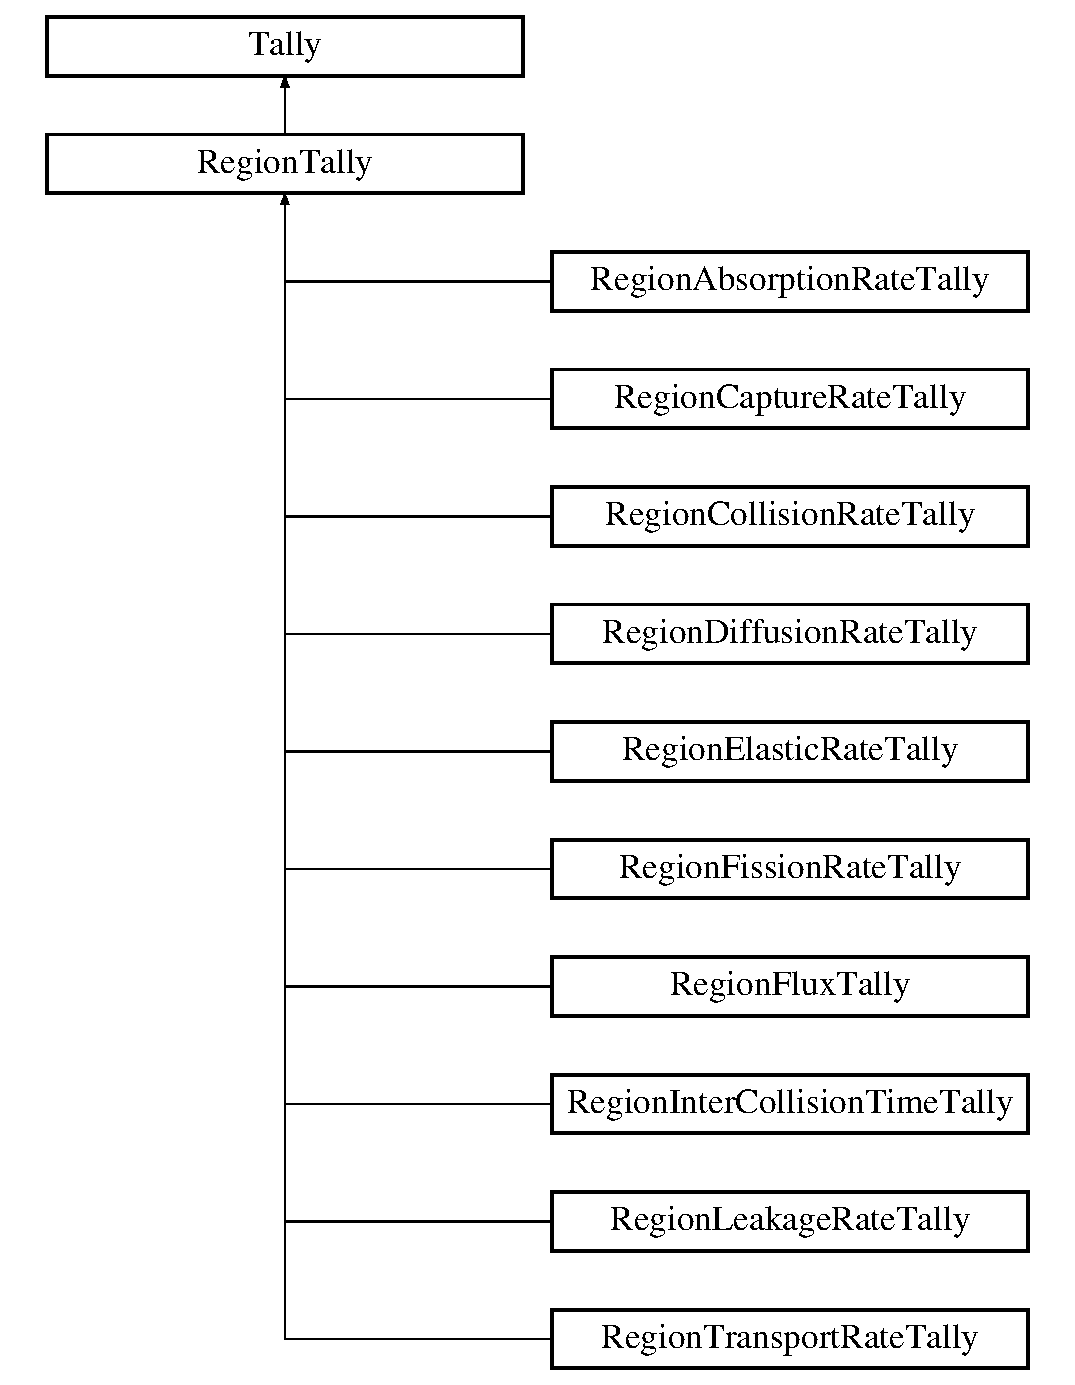
\includegraphics[height=12.000000cm]{classRegionTally}
\end{center}
\end{figure}
\subsection*{Public Member Functions}
\begin{DoxyCompactItemize}
\item 
\hyperlink{classRegionTally_a82b509ab3c69d15f67b3eb1c15b94c11}{Region\-Tally} (\hyperlink{classRegion}{Region} $\ast$region, const char $\ast$tally\-\_\-name=(char $\ast$)\char`\"{}\char`\"{})
\begin{DoxyCompactList}\small\item\em \hyperlink{classRegionTally}{Region\-Tally} constructor calls the \hyperlink{classTally}{Tally} constructor and sets the tally domain to R\-E\-G\-I\-O\-N. \end{DoxyCompactList}\item 
\hyperlink{classRegion}{Region} $\ast$ \hyperlink{classRegionTally_afd80b404adc8b6eaca328f992e23591e}{get\-Region} ()
\begin{DoxyCompactList}\small\item\em Returns the region in which this tally resides. \end{DoxyCompactList}\item 
\hypertarget{classRegionTally_ae146fd937e34306fdd5cc4aac44a3856}{virtual void \hyperlink{classRegionTally_ae146fd937e34306fdd5cc4aac44a3856}{tally} (\hyperlink{structneutron}{neutron} $\ast$\hyperlink{structneutron}{neutron})=0}\label{classRegionTally_ae146fd937e34306fdd5cc4aac44a3856}

\begin{DoxyCompactList}\small\item\em A method to tally a neutron to be implemented by subclasses. \end{DoxyCompactList}\end{DoxyCompactItemize}
\subsection*{Protected Attributes}
\begin{DoxyCompactItemize}
\item 
\hyperlink{classRegion}{Region} $\ast$ \hyperlink{classRegionTally_ac9b5e8a2d01f73c79a22d5d6da0a376d}{\-\_\-region}
\end{DoxyCompactItemize}


\subsection{Detailed Description}
An abstract class for tallies with R\-E\-G\-I\-O\-N domain type. 

A \hyperlink{classRegionTally}{Region\-Tally} is for tallying within a region. The \hyperlink{classRegionTally}{Region\-Tally} is an abstract class and must be implemented for each tally\-Type. 

\subsection{Constructor \& Destructor Documentation}
\hypertarget{classRegionTally_a82b509ab3c69d15f67b3eb1c15b94c11}{\index{Region\-Tally@{Region\-Tally}!Region\-Tally@{Region\-Tally}}
\index{Region\-Tally@{Region\-Tally}!RegionTally@{Region\-Tally}}
\subsubsection[{Region\-Tally}]{\setlength{\rightskip}{0pt plus 5cm}Region\-Tally\-::\-Region\-Tally (
\begin{DoxyParamCaption}
\item[{{\bf Region} $\ast$}]{region, }
\item[{const char $\ast$}]{tally\-\_\-name = {\ttfamily (char$\ast$)\char`\"{}\char`\"{}}}
\end{DoxyParamCaption}
)\hspace{0.3cm}{\ttfamily [inline]}}}\label{classRegionTally_a82b509ab3c69d15f67b3eb1c15b94c11}


\hyperlink{classRegionTally}{Region\-Tally} constructor calls the \hyperlink{classTally}{Tally} constructor and sets the tally domain to R\-E\-G\-I\-O\-N. 


\begin{DoxyParams}{Parameters}
{\em region} & a pointer to the region within which to tally \\
\hline
{\em tally\-\_\-name} & a character array for the tally name (optional) \\
\hline
\end{DoxyParams}


\subsection{Member Function Documentation}
\hypertarget{classRegionTally_afd80b404adc8b6eaca328f992e23591e}{\index{Region\-Tally@{Region\-Tally}!get\-Region@{get\-Region}}
\index{get\-Region@{get\-Region}!RegionTally@{Region\-Tally}}
\subsubsection[{get\-Region}]{\setlength{\rightskip}{0pt plus 5cm}{\bf Region}$\ast$ Region\-Tally\-::get\-Region (
\begin{DoxyParamCaption}
{}
\end{DoxyParamCaption}
)\hspace{0.3cm}{\ttfamily [inline]}}}\label{classRegionTally_afd80b404adc8b6eaca328f992e23591e}


Returns the region in which this tally resides. 

\begin{DoxyReturn}{Returns}
a pointer to the region 
\end{DoxyReturn}


\subsection{Member Data Documentation}
\hypertarget{classRegionTally_ac9b5e8a2d01f73c79a22d5d6da0a376d}{\index{Region\-Tally@{Region\-Tally}!\-\_\-region@{\-\_\-region}}
\index{\-\_\-region@{\-\_\-region}!RegionTally@{Region\-Tally}}
\subsubsection[{\-\_\-region}]{\setlength{\rightskip}{0pt plus 5cm}{\bf Region}$\ast$ Region\-Tally\-::\-\_\-region\hspace{0.3cm}{\ttfamily [protected]}}}\label{classRegionTally_ac9b5e8a2d01f73c79a22d5d6da0a376d}
A pointer to the region in which this tally resides 

The documentation for this class was generated from the following file\-:\begin{DoxyCompactItemize}
\item 
pinspec/src/\hyperlink{Tally_8h}{Tally.\-h}\end{DoxyCompactItemize}

\hypertarget{classRegionTransportRateTally}{\section{Region\-Transport\-Rate\-Tally Class Reference}
\label{classRegionTransportRateTally}\index{Region\-Transport\-Rate\-Tally@{Region\-Transport\-Rate\-Tally}}
}


A class for tallying the transport rate within a region.  




{\ttfamily \#include \char`\"{}pinspec/src/\-Tally.\-h\char`\"{}}

Inheritance diagram for Region\-Transport\-Rate\-Tally\-:\begin{figure}[H]
\begin{center}
\leavevmode
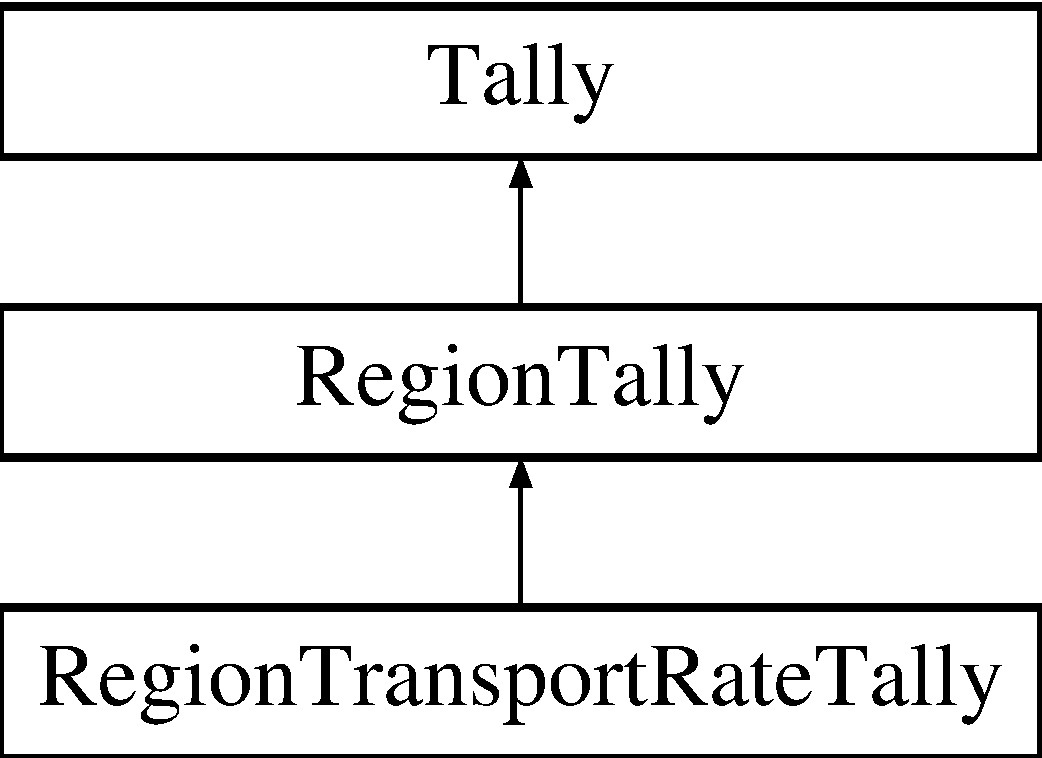
\includegraphics[height=3.000000cm]{classRegionTransportRateTally}
\end{center}
\end{figure}
\subsection*{Public Member Functions}
\begin{DoxyCompactItemize}
\item 
\hyperlink{classRegionTransportRateTally_a7be90fefee298aad00612fdad134a6ea}{Region\-Transport\-Rate\-Tally} (\hyperlink{classRegion}{Region} $\ast$region, const char $\ast$tally\-\_\-name=(char $\ast$)\char`\"{}\char`\"{})
\begin{DoxyCompactList}\small\item\em \hyperlink{classRegionTransportRateTally}{Region\-Transport\-Rate\-Tally} constructor calls the \hyperlink{classRegionTally}{Region\-Tally} constructor and \hyperlink{classTally}{Tally} constructors and sets the tally type to T\-R\-A\-N\-S\-P\-O\-R\-T\-\_\-\-R\-A\-T\-E. \end{DoxyCompactList}\item 
void \hyperlink{classRegionTransportRateTally_af373747c50c56011383dcf569a685af2}{tally} (\hyperlink{structneutron}{neutron} $\ast$\hyperlink{structneutron}{neutron})
\begin{DoxyCompactList}\small\item\em \hyperlink{classTally}{Tally} the region transport rate by incrementing the tally by $ \frac{\Sigma_tr}{\Sigma_t} $ at the neutron's energy. \end{DoxyCompactList}\end{DoxyCompactItemize}
\subsection*{Additional Inherited Members}


\subsection{Detailed Description}
A class for tallying the transport rate within a region. 

\subsection{Constructor \& Destructor Documentation}
\hypertarget{classRegionTransportRateTally_a7be90fefee298aad00612fdad134a6ea}{\index{Region\-Transport\-Rate\-Tally@{Region\-Transport\-Rate\-Tally}!Region\-Transport\-Rate\-Tally@{Region\-Transport\-Rate\-Tally}}
\index{Region\-Transport\-Rate\-Tally@{Region\-Transport\-Rate\-Tally}!RegionTransportRateTally@{Region\-Transport\-Rate\-Tally}}
\subsubsection[{Region\-Transport\-Rate\-Tally}]{\setlength{\rightskip}{0pt plus 5cm}Region\-Transport\-Rate\-Tally\-::\-Region\-Transport\-Rate\-Tally (
\begin{DoxyParamCaption}
\item[{{\bf Region} $\ast$}]{region, }
\item[{const char $\ast$}]{tally\-\_\-name = {\ttfamily (char$\ast$)\char`\"{}\char`\"{}}}
\end{DoxyParamCaption}
)\hspace{0.3cm}{\ttfamily [inline]}}}\label{classRegionTransportRateTally_a7be90fefee298aad00612fdad134a6ea}


\hyperlink{classRegionTransportRateTally}{Region\-Transport\-Rate\-Tally} constructor calls the \hyperlink{classRegionTally}{Region\-Tally} constructor and \hyperlink{classTally}{Tally} constructors and sets the tally type to T\-R\-A\-N\-S\-P\-O\-R\-T\-\_\-\-R\-A\-T\-E. 


\begin{DoxyParams}{Parameters}
{\em region} & a pointer to the region within which to tally \\
\hline
{\em tally\-\_\-name} & a character array for the tally name (optional) \\
\hline
\end{DoxyParams}


\subsection{Member Function Documentation}
\hypertarget{classRegionTransportRateTally_af373747c50c56011383dcf569a685af2}{\index{Region\-Transport\-Rate\-Tally@{Region\-Transport\-Rate\-Tally}!tally@{tally}}
\index{tally@{tally}!RegionTransportRateTally@{Region\-Transport\-Rate\-Tally}}
\subsubsection[{tally}]{\setlength{\rightskip}{0pt plus 5cm}void Region\-Transport\-Rate\-Tally\-::tally (
\begin{DoxyParamCaption}
\item[{{\bf neutron} $\ast$}]{neutron}
\end{DoxyParamCaption}
)\hspace{0.3cm}{\ttfamily [virtual]}}}\label{classRegionTransportRateTally_af373747c50c56011383dcf569a685af2}


\hyperlink{classTally}{Tally} the region transport rate by incrementing the tally by $ \frac{\Sigma_tr}{\Sigma_t} $ at the neutron's energy. 


\begin{DoxyParams}{Parameters}
{\em neutron} & the neutron of interest \\
\hline
\end{DoxyParams}


Implements \hyperlink{classRegionTally_ae146fd937e34306fdd5cc4aac44a3856}{Region\-Tally}.



The documentation for this class was generated from the following files\-:\begin{DoxyCompactItemize}
\item 
\hyperlink{Tally_8h}{Tally.\-h}\item 
Tally.\-cpp\end{DoxyCompactItemize}

\hypertarget{classpinspec_1_1process_1_1RIEff}{\section{pinspec.\-process.\-R\-I\-Eff Class Reference}
\label{classpinspec_1_1process_1_1RIEff}\index{pinspec.\-process.\-R\-I\-Eff@{pinspec.\-process.\-R\-I\-Eff}}
}


An effective resonance integral.  




{\ttfamily \#include \char`\"{}pinspec/process.\-py\char`\"{}}

\subsection*{Public Member Functions}
\begin{DoxyCompactItemize}
\item 
def \hyperlink{classpinspec_1_1process_1_1RIEff_a509b004ebdb23bd0239706108256541c}{\-\_\-\-\_\-init\-\_\-\-\_\-}
\begin{DoxyCompactList}\small\item\em \hyperlink{classpinspec_1_1process_1_1RIEff}{R\-I\-Eff} constructor. \end{DoxyCompactList}\item 
def \hyperlink{classpinspec_1_1process_1_1RIEff_a821baa9dccb3c9a1aa9ebf5c1044059d}{compute\-R\-Is}
\begin{DoxyCompactList}\small\item\em Computes the resonance integrals from the two tallies. \end{DoxyCompactList}\item 
def \hyperlink{classpinspec_1_1process_1_1RIEff_a0a484c374d5285ec12506fc4bbc7f079}{set\-Name}
\begin{DoxyCompactList}\small\item\em Sets the name of this effective resonance integral. \end{DoxyCompactList}\item 
def \hyperlink{classpinspec_1_1process_1_1RIEff_abfe306d889c69c3bf739542617695a0a}{get\-Name}
\begin{DoxyCompactList}\small\item\em Returns the name of the \hyperlink{classpinspec_1_1process_1_1RIEff}{R\-I\-Eff} object. \end{DoxyCompactList}\item 
def \hyperlink{classpinspec_1_1process_1_1RIEff_ade5267dec68494c580c081f69ea91d84}{get\-Num\-Integrals}
\begin{DoxyCompactList}\small\item\em Returns the number of resonance integral energy bands. \end{DoxyCompactList}\item 
def \hyperlink{classpinspec_1_1process_1_1RIEff_a70a5b0c127c6d45b6071b4f4b827f9f0}{get\-Integrals}
\begin{DoxyCompactList}\small\item\em Returns an array of the resonance integral batch averaged values for each tally bin. \end{DoxyCompactList}\item 
def \hyperlink{classpinspec_1_1process_1_1RIEff_a916110ec4e0a682acd4b50aefcc9829c}{get\-Variances}
\begin{DoxyCompactList}\small\item\em Returns an array of the resonance integral batch variances for each tally bin. \end{DoxyCompactList}\item 
def \hyperlink{classpinspec_1_1process_1_1RIEff_a9f30b37d214cb834f2b2fb2f8663d6d4}{get\-Standard\-Deviation}
\begin{DoxyCompactList}\small\item\em Returns an array of the resonance integral batch standard deviations for each tally bin. \end{DoxyCompactList}\item 
def \hyperlink{classpinspec_1_1process_1_1RIEff_a6f44452b15380d62bdbd1fb7cc5c0894}{get\-Relative\-Error}
\begin{DoxyCompactList}\small\item\em Returns an array of the resonance integral batch relative errors for each tally bin. \end{DoxyCompactList}\item 
def \hyperlink{classpinspec_1_1process_1_1RIEff_a3bb8f9f0789d62b5662f181fb1e25b03}{get\-Energy\-Bands\-Centers}
\begin{DoxyCompactList}\small\item\em Returns an array of the resonance integral energy band centers for each tally bin. \end{DoxyCompactList}\item 
def \hyperlink{classpinspec_1_1process_1_1RIEff_a833ecea30944705d16b8ed514de32b2b}{get\-Energy\-Bands}
\begin{DoxyCompactList}\small\item\em Returns an array of the resonance integral energy bands. \end{DoxyCompactList}\item 
def \hyperlink{classpinspec_1_1process_1_1RIEff_a6b661611c10aa686c647f7e81ddb0525}{get\-R\-I\-Tally}
\begin{DoxyCompactList}\small\item\em Returns a reference to this \hyperlink{classpinspec_1_1process_1_1RIEff}{R\-I\-Eff} object. \end{DoxyCompactList}\item 
def \hyperlink{classpinspec_1_1process_1_1RIEff_ac3af925ad0212228c18d2dec7cd6a056}{print\-R\-I}
\begin{DoxyCompactList}\small\item\em Prints a formatted table of the effective resonance integrals to the screen. \end{DoxyCompactList}\item 
def \hyperlink{classpinspec_1_1process_1_1RIEff_a222c27b2e654c5823bbd0293d87a4292}{output\-R\-Ito\-File}
\begin{DoxyCompactList}\small\item\em Prints the resonance integral data and batch statistics to a file. \end{DoxyCompactList}\end{DoxyCompactItemize}
\subsection*{Private Attributes}
\begin{DoxyCompactItemize}
\item 
\hypertarget{classpinspec_1_1process_1_1RIEff_ac301e973346fc58c883b4be4d1dfb16d}{\hyperlink{classpinspec_1_1process_1_1RIEff_ac301e973346fc58c883b4be4d1dfb16d}{\-\_\-name}}\label{classpinspec_1_1process_1_1RIEff_ac301e973346fc58c883b4be4d1dfb16d}

\begin{DoxyCompactList}\small\item\em The name of the effective resonance integral. \end{DoxyCompactList}\item 
\hypertarget{classpinspec_1_1process_1_1RIEff_a05447de3e70c5b7527aed85dbea6391d}{\hyperlink{classpinspec_1_1process_1_1RIEff_a05447de3e70c5b7527aed85dbea6391d}{\-\_\-\-R\-I}}\label{classpinspec_1_1process_1_1RIEff_a05447de3e70c5b7527aed85dbea6391d}

\begin{DoxyCompactList}\small\item\em The D\-E\-R\-I\-V\-E\-D tally type for the effective resonance integral data. \end{DoxyCompactList}\item 
\hypertarget{classpinspec_1_1process_1_1RIEff_af0215d52bf5723c78262906e8c7f08c2}{\hyperlink{classpinspec_1_1process_1_1RIEff_af0215d52bf5723c78262906e8c7f08c2}{\-\_\-flux}}\label{classpinspec_1_1process_1_1RIEff_af0215d52bf5723c78262906e8c7f08c2}

\begin{DoxyCompactList}\small\item\em The F\-L\-U\-X tally used to compute the effective resonance integral. \end{DoxyCompactList}\item 
\hypertarget{classpinspec_1_1process_1_1RIEff_a3f4dc5383e688ba931f0e59217537500}{\hyperlink{classpinspec_1_1process_1_1RIEff_a3f4dc5383e688ba931f0e59217537500}{\-\_\-rate}}\label{classpinspec_1_1process_1_1RIEff_a3f4dc5383e688ba931f0e59217537500}

\begin{DoxyCompactList}\small\item\em The R\-E\-A\-C\-T\-I\-O\-N\-\_\-\-R\-A\-T\-E tally used to compute the effective resonance integral. \end{DoxyCompactList}\item 
\hypertarget{classpinspec_1_1process_1_1RIEff_a3cb90b203ab23c3a8e1d846ab0f722b8}{\hyperlink{classpinspec_1_1process_1_1RIEff_a3cb90b203ab23c3a8e1d846ab0f722b8}{\-\_\-num\-\_\-\-R\-Is}}\label{classpinspec_1_1process_1_1RIEff_a3cb90b203ab23c3a8e1d846ab0f722b8}

\begin{DoxyCompactList}\small\item\em The number of resonance integral energy bands. \end{DoxyCompactList}\end{DoxyCompactItemize}


\subsection{Detailed Description}
An effective resonance integral. 

This class represents an effective resonance integral computed by a P\-I\-N\-S\-P\-E\-C monte carlo simulation. Two tallies -\/ one reaction rate and one flux -\/ are required to form a \hyperlink{classpinspec_1_1process_1_1RIEff}{R\-I\-Eff} class object. 

\subsection{Constructor \& Destructor Documentation}
\hypertarget{classpinspec_1_1process_1_1RIEff_a509b004ebdb23bd0239706108256541c}{\index{pinspec\-::process\-::\-R\-I\-Eff@{pinspec\-::process\-::\-R\-I\-Eff}!\-\_\-\-\_\-init\-\_\-\-\_\-@{\-\_\-\-\_\-init\-\_\-\-\_\-}}
\index{\-\_\-\-\_\-init\-\_\-\-\_\-@{\-\_\-\-\_\-init\-\_\-\-\_\-}!pinspec::process::RIEff@{pinspec\-::process\-::\-R\-I\-Eff}}
\subsubsection[{\-\_\-\-\_\-init\-\_\-\-\_\-}]{\setlength{\rightskip}{0pt plus 5cm}def pinspec.\-process.\-R\-I\-Eff.\-\_\-\-\_\-init\-\_\-\-\_\- (
\begin{DoxyParamCaption}
\item[{}]{self, }
\item[{}]{tally1, }
\item[{}]{tally2, }
\item[{}]{name = {\ttfamily ''}}
\end{DoxyParamCaption}
)}}\label{classpinspec_1_1process_1_1RIEff_a509b004ebdb23bd0239706108256541c}


\hyperlink{classpinspec_1_1process_1_1RIEff}{R\-I\-Eff} constructor. 


\begin{DoxyParams}{Parameters}
{\em self} & the \hyperlink{classpinspec_1_1process_1_1RIEff}{R\-I\-Eff} object pointer \\
\hline
{\em tally1} & one of the tallies needed to compute an $ RI_{eff} $ \\
\hline
{\em tally2} & one of the tallies needed to compute an $ RI_{eff} $ \\
\hline
{\em name} & an optional string for the name of the resonance integral \\
\hline
\end{DoxyParams}


\subsection{Member Function Documentation}
\hypertarget{classpinspec_1_1process_1_1RIEff_a821baa9dccb3c9a1aa9ebf5c1044059d}{\index{pinspec\-::process\-::\-R\-I\-Eff@{pinspec\-::process\-::\-R\-I\-Eff}!compute\-R\-Is@{compute\-R\-Is}}
\index{compute\-R\-Is@{compute\-R\-Is}!pinspec::process::RIEff@{pinspec\-::process\-::\-R\-I\-Eff}}
\subsubsection[{compute\-R\-Is}]{\setlength{\rightskip}{0pt plus 5cm}def pinspec.\-process.\-R\-I\-Eff.\-compute\-R\-Is (
\begin{DoxyParamCaption}
\item[{}]{self, }
\item[{}]{tally1, }
\item[{}]{tally2}
\end{DoxyParamCaption}
)}}\label{classpinspec_1_1process_1_1RIEff_a821baa9dccb3c9a1aa9ebf5c1044059d}


Computes the resonance integrals from the two tallies. 

This method checks that one of the tallies input is a reaction rate and the other is a flux, with the same bin edges. If the batch statistics for both tallies have been computed, it computes the resonance integral as follows\-:


\begin{DoxyCode}
edges = \hyperlink{namespacepinspec_1_1process_a9fd8e784cab1f1c96bd490b212a971c0}{getTallyEdges}(tally1)
log\_array = numpy.log(edges[1:] / edges[0:edges.size-1])
RI\_eff = (reaction\_rate / flux).multiplyDoubles(log\_array)
\end{DoxyCode}



\begin{DoxyParams}{Parameters}
{\em self} & the \hyperlink{classpinspec_1_1process_1_1RIEff}{R\-I\-Eff} object pointer \\
\hline
{\em tally1} & one of the tallies needed to compute an $ RI_{eff} $ \\
\hline
{\em tally2} & one of the tallies needed to compute an $ RI_{eff} $ \\
\hline
\end{DoxyParams}
\hypertarget{classpinspec_1_1process_1_1RIEff_a833ecea30944705d16b8ed514de32b2b}{\index{pinspec\-::process\-::\-R\-I\-Eff@{pinspec\-::process\-::\-R\-I\-Eff}!get\-Energy\-Bands@{get\-Energy\-Bands}}
\index{get\-Energy\-Bands@{get\-Energy\-Bands}!pinspec::process::RIEff@{pinspec\-::process\-::\-R\-I\-Eff}}
\subsubsection[{get\-Energy\-Bands}]{\setlength{\rightskip}{0pt plus 5cm}def pinspec.\-process.\-R\-I\-Eff.\-get\-Energy\-Bands (
\begin{DoxyParamCaption}
\item[{}]{self}
\end{DoxyParamCaption}
)}}\label{classpinspec_1_1process_1_1RIEff_a833ecea30944705d16b8ed514de32b2b}


Returns an array of the resonance integral energy bands. 

The energy bands are the tally bin edges for the reaction rate and flux tally forming this effective resonance integral. 
\begin{DoxyParams}{Parameters}
{\em self} & the \hyperlink{classpinspec_1_1process_1_1RIEff}{R\-I\-Eff} object pointer \\
\hline
\end{DoxyParams}
\begin{DoxyReturn}{Returns}
a numpy array of the resonance integral energy bands (e\-V) 
\end{DoxyReturn}
\hypertarget{classpinspec_1_1process_1_1RIEff_a3bb8f9f0789d62b5662f181fb1e25b03}{\index{pinspec\-::process\-::\-R\-I\-Eff@{pinspec\-::process\-::\-R\-I\-Eff}!get\-Energy\-Bands\-Centers@{get\-Energy\-Bands\-Centers}}
\index{get\-Energy\-Bands\-Centers@{get\-Energy\-Bands\-Centers}!pinspec::process::RIEff@{pinspec\-::process\-::\-R\-I\-Eff}}
\subsubsection[{get\-Energy\-Bands\-Centers}]{\setlength{\rightskip}{0pt plus 5cm}def pinspec.\-process.\-R\-I\-Eff.\-get\-Energy\-Bands\-Centers (
\begin{DoxyParamCaption}
\item[{}]{self}
\end{DoxyParamCaption}
)}}\label{classpinspec_1_1process_1_1RIEff_a3bb8f9f0789d62b5662f181fb1e25b03}


Returns an array of the resonance integral energy band centers for each tally bin. 


\begin{DoxyParams}{Parameters}
{\em self} & the \hyperlink{classpinspec_1_1process_1_1RIEff}{R\-I\-Eff} object pointer \\
\hline
\end{DoxyParams}
\begin{DoxyReturn}{Returns}
a numpy array of the resonance integral energy band centers 
\end{DoxyReturn}
\hypertarget{classpinspec_1_1process_1_1RIEff_a70a5b0c127c6d45b6071b4f4b827f9f0}{\index{pinspec\-::process\-::\-R\-I\-Eff@{pinspec\-::process\-::\-R\-I\-Eff}!get\-Integrals@{get\-Integrals}}
\index{get\-Integrals@{get\-Integrals}!pinspec::process::RIEff@{pinspec\-::process\-::\-R\-I\-Eff}}
\subsubsection[{get\-Integrals}]{\setlength{\rightskip}{0pt plus 5cm}def pinspec.\-process.\-R\-I\-Eff.\-get\-Integrals (
\begin{DoxyParamCaption}
\item[{}]{self}
\end{DoxyParamCaption}
)}}\label{classpinspec_1_1process_1_1RIEff_a70a5b0c127c6d45b6071b4f4b827f9f0}


Returns an array of the resonance integral batch averaged values for each tally bin. 


\begin{DoxyParams}{Parameters}
{\em self} & the \hyperlink{classpinspec_1_1process_1_1RIEff}{R\-I\-Eff} object pointer \\
\hline
\end{DoxyParams}
\begin{DoxyReturn}{Returns}
a numpy array of the resonance integrals 
\end{DoxyReturn}
\hypertarget{classpinspec_1_1process_1_1RIEff_abfe306d889c69c3bf739542617695a0a}{\index{pinspec\-::process\-::\-R\-I\-Eff@{pinspec\-::process\-::\-R\-I\-Eff}!get\-Name@{get\-Name}}
\index{get\-Name@{get\-Name}!pinspec::process::RIEff@{pinspec\-::process\-::\-R\-I\-Eff}}
\subsubsection[{get\-Name}]{\setlength{\rightskip}{0pt plus 5cm}def pinspec.\-process.\-R\-I\-Eff.\-get\-Name (
\begin{DoxyParamCaption}
\item[{}]{self}
\end{DoxyParamCaption}
)}}\label{classpinspec_1_1process_1_1RIEff_abfe306d889c69c3bf739542617695a0a}


Returns the name of the \hyperlink{classpinspec_1_1process_1_1RIEff}{R\-I\-Eff} object. 

Returns an empty string if no name has been specified by the user. 
\begin{DoxyParams}{Parameters}
{\em self} & the \hyperlink{classpinspec_1_1process_1_1RIEff}{R\-I\-Eff} object pointer \\
\hline
\end{DoxyParams}
\begin{DoxyReturn}{Returns}
a string with the name of the \hyperlink{classpinspec_1_1process_1_1RIEff}{R\-I\-Eff} 
\end{DoxyReturn}
\hypertarget{classpinspec_1_1process_1_1RIEff_ade5267dec68494c580c081f69ea91d84}{\index{pinspec\-::process\-::\-R\-I\-Eff@{pinspec\-::process\-::\-R\-I\-Eff}!get\-Num\-Integrals@{get\-Num\-Integrals}}
\index{get\-Num\-Integrals@{get\-Num\-Integrals}!pinspec::process::RIEff@{pinspec\-::process\-::\-R\-I\-Eff}}
\subsubsection[{get\-Num\-Integrals}]{\setlength{\rightskip}{0pt plus 5cm}def pinspec.\-process.\-R\-I\-Eff.\-get\-Num\-Integrals (
\begin{DoxyParamCaption}
\item[{}]{self}
\end{DoxyParamCaption}
)}}\label{classpinspec_1_1process_1_1RIEff_ade5267dec68494c580c081f69ea91d84}


Returns the number of resonance integral energy bands. 

The number of integrals is equivalent to the number of tally bins for the reaction rate and flux tallies. 
\begin{DoxyParams}{Parameters}
{\em self} & the \hyperlink{classpinspec_1_1process_1_1RIEff}{R\-I\-Eff} object pointer \\
\hline
\end{DoxyParams}
\begin{DoxyReturn}{Returns}
the number of resonance integrals 
\end{DoxyReturn}
\hypertarget{classpinspec_1_1process_1_1RIEff_a6f44452b15380d62bdbd1fb7cc5c0894}{\index{pinspec\-::process\-::\-R\-I\-Eff@{pinspec\-::process\-::\-R\-I\-Eff}!get\-Relative\-Error@{get\-Relative\-Error}}
\index{get\-Relative\-Error@{get\-Relative\-Error}!pinspec::process::RIEff@{pinspec\-::process\-::\-R\-I\-Eff}}
\subsubsection[{get\-Relative\-Error}]{\setlength{\rightskip}{0pt plus 5cm}def pinspec.\-process.\-R\-I\-Eff.\-get\-Relative\-Error (
\begin{DoxyParamCaption}
\item[{}]{self}
\end{DoxyParamCaption}
)}}\label{classpinspec_1_1process_1_1RIEff_a6f44452b15380d62bdbd1fb7cc5c0894}


Returns an array of the resonance integral batch relative errors for each tally bin. 


\begin{DoxyParams}{Parameters}
{\em self} & the \hyperlink{classpinspec_1_1process_1_1RIEff}{R\-I\-Eff} object pointer \\
\hline
\end{DoxyParams}
\begin{DoxyReturn}{Returns}
a numpy array of the resonance integral relative errors 
\end{DoxyReturn}
\hypertarget{classpinspec_1_1process_1_1RIEff_a6b661611c10aa686c647f7e81ddb0525}{\index{pinspec\-::process\-::\-R\-I\-Eff@{pinspec\-::process\-::\-R\-I\-Eff}!get\-R\-I\-Tally@{get\-R\-I\-Tally}}
\index{get\-R\-I\-Tally@{get\-R\-I\-Tally}!pinspec::process::RIEff@{pinspec\-::process\-::\-R\-I\-Eff}}
\subsubsection[{get\-R\-I\-Tally}]{\setlength{\rightskip}{0pt plus 5cm}def pinspec.\-process.\-R\-I\-Eff.\-get\-R\-I\-Tally (
\begin{DoxyParamCaption}
\item[{}]{self}
\end{DoxyParamCaption}
)}}\label{classpinspec_1_1process_1_1RIEff_a6b661611c10aa686c647f7e81ddb0525}


Returns a reference to this \hyperlink{classpinspec_1_1process_1_1RIEff}{R\-I\-Eff} object. 


\begin{DoxyParams}{Parameters}
{\em self} & \hyperlink{classpinspec_1_1process_1_1RIEff}{R\-I\-Eff} the object pointer \\
\hline
\end{DoxyParams}
\begin{DoxyReturn}{Returns}
a reference to the \hyperlink{classpinspec_1_1process_1_1RIEff}{R\-I\-Eff} object 
\end{DoxyReturn}
\hypertarget{classpinspec_1_1process_1_1RIEff_a9f30b37d214cb834f2b2fb2f8663d6d4}{\index{pinspec\-::process\-::\-R\-I\-Eff@{pinspec\-::process\-::\-R\-I\-Eff}!get\-Standard\-Deviation@{get\-Standard\-Deviation}}
\index{get\-Standard\-Deviation@{get\-Standard\-Deviation}!pinspec::process::RIEff@{pinspec\-::process\-::\-R\-I\-Eff}}
\subsubsection[{get\-Standard\-Deviation}]{\setlength{\rightskip}{0pt plus 5cm}def pinspec.\-process.\-R\-I\-Eff.\-get\-Standard\-Deviation (
\begin{DoxyParamCaption}
\item[{}]{self}
\end{DoxyParamCaption}
)}}\label{classpinspec_1_1process_1_1RIEff_a9f30b37d214cb834f2b2fb2f8663d6d4}


Returns an array of the resonance integral batch standard deviations for each tally bin. 


\begin{DoxyParams}{Parameters}
{\em self} & the \hyperlink{classpinspec_1_1process_1_1RIEff}{R\-I\-Eff} object pointer \\
\hline
\end{DoxyParams}
\begin{DoxyReturn}{Returns}
a numpy array of the resonance integral standard deviations 
\end{DoxyReturn}
\hypertarget{classpinspec_1_1process_1_1RIEff_a916110ec4e0a682acd4b50aefcc9829c}{\index{pinspec\-::process\-::\-R\-I\-Eff@{pinspec\-::process\-::\-R\-I\-Eff}!get\-Variances@{get\-Variances}}
\index{get\-Variances@{get\-Variances}!pinspec::process::RIEff@{pinspec\-::process\-::\-R\-I\-Eff}}
\subsubsection[{get\-Variances}]{\setlength{\rightskip}{0pt plus 5cm}def pinspec.\-process.\-R\-I\-Eff.\-get\-Variances (
\begin{DoxyParamCaption}
\item[{}]{self}
\end{DoxyParamCaption}
)}}\label{classpinspec_1_1process_1_1RIEff_a916110ec4e0a682acd4b50aefcc9829c}


Returns an array of the resonance integral batch variances for each tally bin. 


\begin{DoxyParams}{Parameters}
{\em self} & the \hyperlink{classpinspec_1_1process_1_1RIEff}{R\-I\-Eff} object pointer \\
\hline
\end{DoxyParams}
\begin{DoxyReturn}{Returns}
a numpy array of the resonance integral variances 
\end{DoxyReturn}
\hypertarget{classpinspec_1_1process_1_1RIEff_a222c27b2e654c5823bbd0293d87a4292}{\index{pinspec\-::process\-::\-R\-I\-Eff@{pinspec\-::process\-::\-R\-I\-Eff}!output\-R\-Ito\-File@{output\-R\-Ito\-File}}
\index{output\-R\-Ito\-File@{output\-R\-Ito\-File}!pinspec::process::RIEff@{pinspec\-::process\-::\-R\-I\-Eff}}
\subsubsection[{output\-R\-Ito\-File}]{\setlength{\rightskip}{0pt plus 5cm}def pinspec.\-process.\-R\-I\-Eff.\-output\-R\-Ito\-File (
\begin{DoxyParamCaption}
\item[{}]{self, }
\item[{}]{filename = {\ttfamily ''}}
\end{DoxyParamCaption}
)}}\label{classpinspec_1_1process_1_1RIEff_a222c27b2e654c5823bbd0293d87a4292}


Prints the resonance integral data and batch statistics to a file. 

Since the effective resonance integral is stored as a D\-E\-R\-I\-V\-E\-D tally type, this method prints the resonance integral data to a file using the \hyperlink{classTally_a4fd93a5423286a5a9b7953cc8d1dcbcf}{Tally\-::output\-Batch\-Statistics()} method. An auto-\/generated filename will be created with the format 'tally-\/\#.data' where \# is an auto-\/incremented integer for each tally output data file created. 
\begin{DoxyParams}{Parameters}
{\em self} & the \hyperlink{classpinspec_1_1process_1_1RIEff}{R\-I\-Eff} object pointer \\
\hline
{\em filename} & An optional filename for the output file \\
\hline
\end{DoxyParams}
\hypertarget{classpinspec_1_1process_1_1RIEff_ac3af925ad0212228c18d2dec7cd6a056}{\index{pinspec\-::process\-::\-R\-I\-Eff@{pinspec\-::process\-::\-R\-I\-Eff}!print\-R\-I@{print\-R\-I}}
\index{print\-R\-I@{print\-R\-I}!pinspec::process::RIEff@{pinspec\-::process\-::\-R\-I\-Eff}}
\subsubsection[{print\-R\-I}]{\setlength{\rightskip}{0pt plus 5cm}def pinspec.\-process.\-R\-I\-Eff.\-print\-R\-I (
\begin{DoxyParamCaption}
\item[{}]{self, }
\item[{}]{uncertainties = {\ttfamily False}}
\end{DoxyParamCaption}
)}}\label{classpinspec_1_1process_1_1RIEff_ac3af925ad0212228c18d2dec7cd6a056}


Prints a formatted table of the effective resonance integrals to the screen. 

The resonance integrals and their uncertainties (optional) will be printed as a formatted table to the screen. 
\begin{DoxyParams}{Parameters}
{\em self} & the \hyperlink{classpinspec_1_1process_1_1RIEff}{R\-I\-Eff} object pointer \\
\hline
{\em uncertainties} & whether or not to print tally statistics (default is false) \\
\hline
\end{DoxyParams}
\begin{DoxyReturn}{Returns}
a reference to the \hyperlink{classpinspec_1_1process_1_1RIEff}{R\-I\-Eff} object 
\end{DoxyReturn}
\hypertarget{classpinspec_1_1process_1_1RIEff_a0a484c374d5285ec12506fc4bbc7f079}{\index{pinspec\-::process\-::\-R\-I\-Eff@{pinspec\-::process\-::\-R\-I\-Eff}!set\-Name@{set\-Name}}
\index{set\-Name@{set\-Name}!pinspec::process::RIEff@{pinspec\-::process\-::\-R\-I\-Eff}}
\subsubsection[{set\-Name}]{\setlength{\rightskip}{0pt plus 5cm}def pinspec.\-process.\-R\-I\-Eff.\-set\-Name (
\begin{DoxyParamCaption}
\item[{}]{self, }
\item[{}]{name = {\ttfamily ''}}
\end{DoxyParamCaption}
)}}\label{classpinspec_1_1process_1_1RIEff_a0a484c374d5285ec12506fc4bbc7f079}


Sets the name of this effective resonance integral. 

This is useful when one wishes to print the resonance integral values to the screen or a file since it will be identifiable by the user-\/defined name. 
\begin{DoxyParams}{Parameters}
{\em self} & the \hyperlink{classpinspec_1_1process_1_1RIEff}{R\-I\-Eff} object pointer \\
\hline
{\em name} & the name of the \hyperlink{classpinspec_1_1process_1_1RIEff}{R\-I\-Eff} object \\
\hline
\end{DoxyParams}


The documentation for this class was generated from the following file\-:\begin{DoxyCompactItemize}
\item 
pinspec/\hyperlink{process_8py}{process.\-py}\end{DoxyCompactItemize}

\hypertarget{classpinspec_1_1process_1_1RITrue}{\section{pinspec.\-process.\-R\-I\-True Class Reference}
\label{classpinspec_1_1process_1_1RITrue}\index{pinspec.\-process.\-R\-I\-True@{pinspec.\-process.\-R\-I\-True}}
}


A true resonance integral.  




{\ttfamily \#include \char`\"{}pinspec/process.\-py\char`\"{}}

\subsection*{Public Member Functions}
\begin{DoxyCompactItemize}
\item 
def \hyperlink{classpinspec_1_1process_1_1RITrue_ab6e86b3e2972731d8d2686e550e87ec8}{\-\_\-\-\_\-init\-\_\-\-\_\-}
\begin{DoxyCompactList}\small\item\em \hyperlink{classpinspec_1_1process_1_1RITrue}{R\-I\-True} constructor. \end{DoxyCompactList}\item 
def \hyperlink{classpinspec_1_1process_1_1RITrue_ad356c85340b6b981a9687a95aa57a375}{set\-Name}
\begin{DoxyCompactList}\small\item\em Sets the name of the true resonance integral. \end{DoxyCompactList}\item 
def \hyperlink{classpinspec_1_1process_1_1RITrue_a23b3e3deabb334457c82c7b4e29d3cf1}{compute\-R\-Is}
\begin{DoxyCompactList}\small\item\em Computes the true resonance integrals for an isotopic reaction rate. \end{DoxyCompactList}\item 
def \hyperlink{classpinspec_1_1process_1_1RITrue_aac61143b201fda62c0a9e1534716dea2}{get\-Name}
\begin{DoxyCompactList}\small\item\em Returns the name of the \hyperlink{classpinspec_1_1process_1_1RITrue}{R\-I\-True} object. \end{DoxyCompactList}\item 
def \hyperlink{classpinspec_1_1process_1_1RITrue_a53316a20b63e3576734fb91f65734e33}{get\-Num\-Integrals}
\begin{DoxyCompactList}\small\item\em Returns the number of resonance integral energy bands. \end{DoxyCompactList}\item 
def \hyperlink{classpinspec_1_1process_1_1RITrue_a5aa42d3c5b4d313f8dee9e56ffe42dd3}{get\-Integrals}
\begin{DoxyCompactList}\small\item\em Returns an array of the resonance integrals for each energy band. \end{DoxyCompactList}\item 
def \hyperlink{classpinspec_1_1process_1_1RITrue_a0fc3d14d394d10c5ec93fd2933d4e82e}{get\-Energy\-Bands\-Centers}
\begin{DoxyCompactList}\small\item\em Returns an array of the centers of each energy band. \end{DoxyCompactList}\item 
def \hyperlink{classpinspec_1_1process_1_1RITrue_a338c2ef0063836581497f4ab957d3a77}{get\-Energy\-Bands}
\begin{DoxyCompactList}\small\item\em Returns an array of the energy bands. \end{DoxyCompactList}\item 
def \hyperlink{classpinspec_1_1process_1_1RITrue_a306c5e00b9d9999020e6b27f4ff7e89d}{print\-R\-Is}
\begin{DoxyCompactList}\small\item\em Prints a formatted table of the true resonance integrals to the screen. \end{DoxyCompactList}\end{DoxyCompactItemize}
\subsection*{Private Attributes}
\begin{DoxyCompactItemize}
\item 
\hypertarget{classpinspec_1_1process_1_1RITrue_aec037fce18c6deae420b010206535fd1}{\hyperlink{classpinspec_1_1process_1_1RITrue_aec037fce18c6deae420b010206535fd1}{\-\_\-name}}\label{classpinspec_1_1process_1_1RITrue_aec037fce18c6deae420b010206535fd1}

\begin{DoxyCompactList}\small\item\em The name of the effective resonance integral. \end{DoxyCompactList}\item 
\hypertarget{classpinspec_1_1process_1_1RITrue_a9bba42c02cf6b46cc92173027fcfc797}{\hyperlink{classpinspec_1_1process_1_1RITrue_a9bba42c02cf6b46cc92173027fcfc797}{\-\_\-isotope}}\label{classpinspec_1_1process_1_1RITrue_a9bba42c02cf6b46cc92173027fcfc797}

\begin{DoxyCompactList}\small\item\em The isotope for this resonance integral. \end{DoxyCompactList}\item 
\hyperlink{classpinspec_1_1process_1_1RITrue_aee6f864082130f6580a2e6173593bdcf}{\-\_\-reaction}
\begin{DoxyCompactList}\small\item\em The reaction rate for this resonance integral (ie, 'capture') \end{DoxyCompactList}\item 
\hypertarget{classpinspec_1_1process_1_1RITrue_a6057570aeb3e2f5f1c8708b515d62401}{\hyperlink{classpinspec_1_1process_1_1RITrue_a6057570aeb3e2f5f1c8708b515d62401}{\-\_\-num\-\_\-\-R\-Is}}\label{classpinspec_1_1process_1_1RITrue_a6057570aeb3e2f5f1c8708b515d62401}

\begin{DoxyCompactList}\small\item\em The number of resonance integrals. \end{DoxyCompactList}\item 
\hypertarget{classpinspec_1_1process_1_1RITrue_a67e6e7f47d4db1c6625a7d3359e87eaf}{\hyperlink{classpinspec_1_1process_1_1RITrue_a67e6e7f47d4db1c6625a7d3359e87eaf}{\-\_\-\-R\-Is}}\label{classpinspec_1_1process_1_1RITrue_a67e6e7f47d4db1c6625a7d3359e87eaf}

\begin{DoxyCompactList}\small\item\em The numpy array of resonance integral values. \end{DoxyCompactList}\item 
\hypertarget{classpinspec_1_1process_1_1RITrue_a147126838dbc1d2a2c5601ff93c21bb4}{\hyperlink{classpinspec_1_1process_1_1RITrue_a147126838dbc1d2a2c5601ff93c21bb4}{\-\_\-energy\-\_\-bands}}\label{classpinspec_1_1process_1_1RITrue_a147126838dbc1d2a2c5601ff93c21bb4}

\begin{DoxyCompactList}\small\item\em The numpy array of energy band values. \end{DoxyCompactList}\end{DoxyCompactItemize}


\subsection{Detailed Description}
A true resonance integral. 

This class represents the true resonance integral computed from a $ \frac{1}{E} $ spectrum. 

\subsection{Constructor \& Destructor Documentation}
\hypertarget{classpinspec_1_1process_1_1RITrue_ab6e86b3e2972731d8d2686e550e87ec8}{\index{pinspec\-::process\-::\-R\-I\-True@{pinspec\-::process\-::\-R\-I\-True}!\-\_\-\-\_\-init\-\_\-\-\_\-@{\-\_\-\-\_\-init\-\_\-\-\_\-}}
\index{\-\_\-\-\_\-init\-\_\-\-\_\-@{\-\_\-\-\_\-init\-\_\-\-\_\-}!pinspec::process::RITrue@{pinspec\-::process\-::\-R\-I\-True}}
\subsubsection[{\-\_\-\-\_\-init\-\_\-\-\_\-}]{\setlength{\rightskip}{0pt plus 5cm}def pinspec.\-process.\-R\-I\-True.\-\_\-\-\_\-init\-\_\-\-\_\- (
\begin{DoxyParamCaption}
\item[{}]{self, }
\item[{}]{isotope, }
\item[{}]{bands, }
\item[{}]{reaction = {\ttfamily 'capture'}, }
\item[{}]{name = {\ttfamily ''}}
\end{DoxyParamCaption}
)}}\label{classpinspec_1_1process_1_1RITrue_ab6e86b3e2972731d8d2686e550e87ec8}


\hyperlink{classpinspec_1_1process_1_1RITrue}{R\-I\-True} constructor. 


\begin{DoxyParams}{Parameters}
{\em self} & the \hyperlink{classpinspec_1_1process_1_1RITrue}{R\-I\-True} object pointer \\
\hline
{\em isotope} & a pointer to the isotope of interest \\
\hline
{\em bands} & an array of the energy bands for each resonance integral \\
\hline
{\em reaction} & an optional argument string with the reaction rate type \\
\hline
{\em name} & an optional argument string for the resonance integral name \\
\hline
\end{DoxyParams}


\subsection{Member Function Documentation}
\hypertarget{classpinspec_1_1process_1_1RITrue_a23b3e3deabb334457c82c7b4e29d3cf1}{\index{pinspec\-::process\-::\-R\-I\-True@{pinspec\-::process\-::\-R\-I\-True}!compute\-R\-Is@{compute\-R\-Is}}
\index{compute\-R\-Is@{compute\-R\-Is}!pinspec::process::RITrue@{pinspec\-::process\-::\-R\-I\-True}}
\subsubsection[{compute\-R\-Is}]{\setlength{\rightskip}{0pt plus 5cm}def pinspec.\-process.\-R\-I\-True.\-compute\-R\-Is (
\begin{DoxyParamCaption}
\item[{}]{self, }
\item[{}]{bands, }
\item[{}]{reaction}
\end{DoxyParamCaption}
)}}\label{classpinspec_1_1process_1_1RITrue_a23b3e3deabb334457c82c7b4e29d3cf1}


Computes the true resonance integrals for an isotopic reaction rate. 

This method computes an infinite dilute resonance integral for each of the user-\/defined energy bands for some isotopic reaction rate using numerical integration as follows\-:

$ \int\limits_{E_{i-1}}^{E_i} \sigma_{j}(E) \frac{1}{E} \mathrm{d}E $


\begin{DoxyParams}{Parameters}
{\em self} & the \hyperlink{classpinspec_1_1process_1_1RITrue}{R\-I\-True} object pointer \\
\hline
{\em bands} & an array of the energy bands for each resonance integral \\
\hline
{\em reaction} & an optional argument string with the reaction rate type \\
\hline
\end{DoxyParams}
\hypertarget{classpinspec_1_1process_1_1RITrue_a338c2ef0063836581497f4ab957d3a77}{\index{pinspec\-::process\-::\-R\-I\-True@{pinspec\-::process\-::\-R\-I\-True}!get\-Energy\-Bands@{get\-Energy\-Bands}}
\index{get\-Energy\-Bands@{get\-Energy\-Bands}!pinspec::process::RITrue@{pinspec\-::process\-::\-R\-I\-True}}
\subsubsection[{get\-Energy\-Bands}]{\setlength{\rightskip}{0pt plus 5cm}def pinspec.\-process.\-R\-I\-True.\-get\-Energy\-Bands (
\begin{DoxyParamCaption}
\item[{}]{self}
\end{DoxyParamCaption}
)}}\label{classpinspec_1_1process_1_1RITrue_a338c2ef0063836581497f4ab957d3a77}


Returns an array of the energy bands. 


\begin{DoxyParams}{Parameters}
{\em self} & the \hyperlink{classpinspec_1_1process_1_1RITrue}{R\-I\-True} object pointer \\
\hline
\end{DoxyParams}
\begin{DoxyReturn}{Returns}
a numpy array of the values defining the energy bands (e\-V) 
\end{DoxyReturn}
\hypertarget{classpinspec_1_1process_1_1RITrue_a0fc3d14d394d10c5ec93fd2933d4e82e}{\index{pinspec\-::process\-::\-R\-I\-True@{pinspec\-::process\-::\-R\-I\-True}!get\-Energy\-Bands\-Centers@{get\-Energy\-Bands\-Centers}}
\index{get\-Energy\-Bands\-Centers@{get\-Energy\-Bands\-Centers}!pinspec::process::RITrue@{pinspec\-::process\-::\-R\-I\-True}}
\subsubsection[{get\-Energy\-Bands\-Centers}]{\setlength{\rightskip}{0pt plus 5cm}def pinspec.\-process.\-R\-I\-True.\-get\-Energy\-Bands\-Centers (
\begin{DoxyParamCaption}
\item[{}]{self}
\end{DoxyParamCaption}
)}}\label{classpinspec_1_1process_1_1RITrue_a0fc3d14d394d10c5ec93fd2933d4e82e}


Returns an array of the centers of each energy band. 


\begin{DoxyParams}{Parameters}
{\em self} & the \hyperlink{classpinspec_1_1process_1_1RITrue}{R\-I\-True} object pointer \\
\hline
\end{DoxyParams}
\begin{DoxyReturn}{Returns}
a numpy array of the energy band centers (e\-V) 
\end{DoxyReturn}
\hypertarget{classpinspec_1_1process_1_1RITrue_a5aa42d3c5b4d313f8dee9e56ffe42dd3}{\index{pinspec\-::process\-::\-R\-I\-True@{pinspec\-::process\-::\-R\-I\-True}!get\-Integrals@{get\-Integrals}}
\index{get\-Integrals@{get\-Integrals}!pinspec::process::RITrue@{pinspec\-::process\-::\-R\-I\-True}}
\subsubsection[{get\-Integrals}]{\setlength{\rightskip}{0pt plus 5cm}def pinspec.\-process.\-R\-I\-True.\-get\-Integrals (
\begin{DoxyParamCaption}
\item[{}]{self}
\end{DoxyParamCaption}
)}}\label{classpinspec_1_1process_1_1RITrue_a5aa42d3c5b4d313f8dee9e56ffe42dd3}


Returns an array of the resonance integrals for each energy band. 


\begin{DoxyParams}{Parameters}
{\em self} & the \hyperlink{classpinspec_1_1process_1_1RITrue}{R\-I\-True} object pointer \\
\hline
\end{DoxyParams}
\begin{DoxyReturn}{Returns}
a numpy array of the resonance integrals 
\end{DoxyReturn}
\hypertarget{classpinspec_1_1process_1_1RITrue_aac61143b201fda62c0a9e1534716dea2}{\index{pinspec\-::process\-::\-R\-I\-True@{pinspec\-::process\-::\-R\-I\-True}!get\-Name@{get\-Name}}
\index{get\-Name@{get\-Name}!pinspec::process::RITrue@{pinspec\-::process\-::\-R\-I\-True}}
\subsubsection[{get\-Name}]{\setlength{\rightskip}{0pt plus 5cm}def pinspec.\-process.\-R\-I\-True.\-get\-Name (
\begin{DoxyParamCaption}
\item[{}]{self}
\end{DoxyParamCaption}
)}}\label{classpinspec_1_1process_1_1RITrue_aac61143b201fda62c0a9e1534716dea2}


Returns the name of the \hyperlink{classpinspec_1_1process_1_1RITrue}{R\-I\-True} object. 

Returns an empty string if no name has been specified by the user. 
\begin{DoxyParams}{Parameters}
{\em self} & the \hyperlink{classpinspec_1_1process_1_1RITrue}{R\-I\-True} object pointer \\
\hline
\end{DoxyParams}
\begin{DoxyReturn}{Returns}
a string with the name of the \hyperlink{classpinspec_1_1process_1_1RITrue}{R\-I\-True} 
\end{DoxyReturn}
\hypertarget{classpinspec_1_1process_1_1RITrue_a53316a20b63e3576734fb91f65734e33}{\index{pinspec\-::process\-::\-R\-I\-True@{pinspec\-::process\-::\-R\-I\-True}!get\-Num\-Integrals@{get\-Num\-Integrals}}
\index{get\-Num\-Integrals@{get\-Num\-Integrals}!pinspec::process::RITrue@{pinspec\-::process\-::\-R\-I\-True}}
\subsubsection[{get\-Num\-Integrals}]{\setlength{\rightskip}{0pt plus 5cm}def pinspec.\-process.\-R\-I\-True.\-get\-Num\-Integrals (
\begin{DoxyParamCaption}
\item[{}]{self}
\end{DoxyParamCaption}
)}}\label{classpinspec_1_1process_1_1RITrue_a53316a20b63e3576734fb91f65734e33}


Returns the number of resonance integral energy bands. 


\begin{DoxyParams}{Parameters}
{\em self} & the \hyperlink{classpinspec_1_1process_1_1RITrue}{R\-I\-True} object pointer \\
\hline
\end{DoxyParams}
\begin{DoxyReturn}{Returns}
the number of resonance integrals 
\end{DoxyReturn}
\hypertarget{classpinspec_1_1process_1_1RITrue_a306c5e00b9d9999020e6b27f4ff7e89d}{\index{pinspec\-::process\-::\-R\-I\-True@{pinspec\-::process\-::\-R\-I\-True}!print\-R\-Is@{print\-R\-Is}}
\index{print\-R\-Is@{print\-R\-Is}!pinspec::process::RITrue@{pinspec\-::process\-::\-R\-I\-True}}
\subsubsection[{print\-R\-Is}]{\setlength{\rightskip}{0pt plus 5cm}def pinspec.\-process.\-R\-I\-True.\-print\-R\-Is (
\begin{DoxyParamCaption}
\item[{}]{self}
\end{DoxyParamCaption}
)}}\label{classpinspec_1_1process_1_1RITrue_a306c5e00b9d9999020e6b27f4ff7e89d}


Prints a formatted table of the true resonance integrals to the screen. 


\begin{DoxyParams}{Parameters}
{\em self} & the \hyperlink{classpinspec_1_1process_1_1RITrue}{R\-I\-True} object pointer \\
\hline
\end{DoxyParams}
\begin{DoxyReturn}{Returns}
a reference to the \hyperlink{classpinspec_1_1process_1_1RITrue}{R\-I\-True} object 
\end{DoxyReturn}
\hypertarget{classpinspec_1_1process_1_1RITrue_ad356c85340b6b981a9687a95aa57a375}{\index{pinspec\-::process\-::\-R\-I\-True@{pinspec\-::process\-::\-R\-I\-True}!set\-Name@{set\-Name}}
\index{set\-Name@{set\-Name}!pinspec::process::RITrue@{pinspec\-::process\-::\-R\-I\-True}}
\subsubsection[{set\-Name}]{\setlength{\rightskip}{0pt plus 5cm}def pinspec.\-process.\-R\-I\-True.\-set\-Name (
\begin{DoxyParamCaption}
\item[{}]{self, }
\item[{}]{name = {\ttfamily ''}}
\end{DoxyParamCaption}
)}}\label{classpinspec_1_1process_1_1RITrue_ad356c85340b6b981a9687a95aa57a375}


Sets the name of the true resonance integral. 

This is useful when one wishes to print the resonance integral values to the screen or a file since it will be identifiable by the user-\/defined name. 
\begin{DoxyParams}{Parameters}
{\em self} & the \hyperlink{classpinspec_1_1process_1_1RITrue}{R\-I\-True} object pointer \\
\hline
{\em name} & the name of the \hyperlink{classpinspec_1_1process_1_1RITrue}{R\-I\-True} object \\
\hline
\end{DoxyParams}


\subsection{Member Data Documentation}
\hypertarget{classpinspec_1_1process_1_1RITrue_aee6f864082130f6580a2e6173593bdcf}{\index{pinspec\-::process\-::\-R\-I\-True@{pinspec\-::process\-::\-R\-I\-True}!\-\_\-reaction@{\-\_\-reaction}}
\index{\-\_\-reaction@{\-\_\-reaction}!pinspec::process::RITrue@{pinspec\-::process\-::\-R\-I\-True}}
\subsubsection[{\-\_\-reaction}]{\setlength{\rightskip}{0pt plus 5cm}pinspec.\-process.\-R\-I\-True.\-\_\-reaction\hspace{0.3cm}{\ttfamily [private]}}}\label{classpinspec_1_1process_1_1RITrue_aee6f864082130f6580a2e6173593bdcf}


The reaction rate for this resonance integral (ie, 'capture') 

The reaction rate type (ie, 'capture') 

The documentation for this class was generated from the following file\-:\begin{DoxyCompactItemize}
\item 
pinspec/\hyperlink{process_8py}{process.\-py}\end{DoxyCompactItemize}

\hypertarget{classSurface}{\section{Surface Class Reference}
\label{classSurface}\index{Surface@{Surface}}
}


The \hyperlink{classSurface}{Surface} represents a quadratic surface in the xy-\/plane.  




{\ttfamily \#include \char`\"{}pinspec/src/\-Surface.\-h\char`\"{}}

Inheritance diagram for Surface\-:\begin{figure}[H]
\begin{center}
\leavevmode
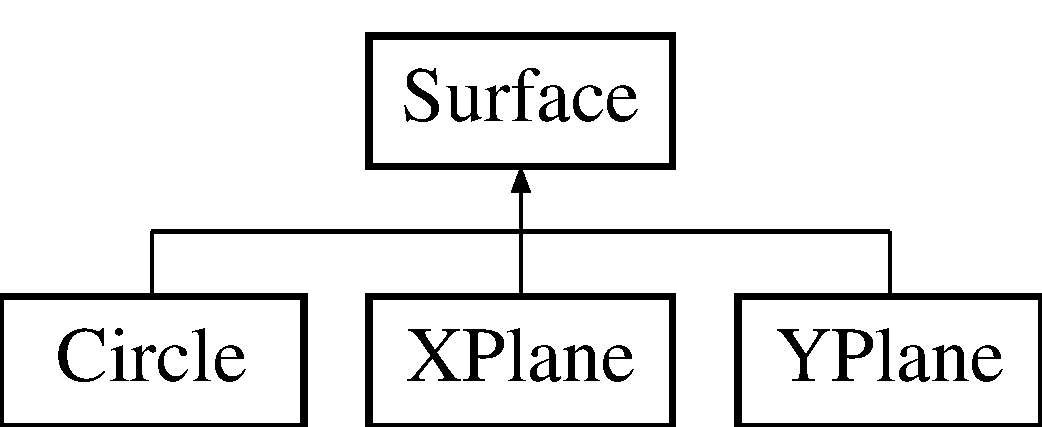
\includegraphics[height=2.000000cm]{classSurface}
\end{center}
\end{figure}
\subsection*{Public Member Functions}
\begin{DoxyCompactItemize}
\item 
\hyperlink{classSurface_a8fc57f2a15292135c00545c9d224ec68}{Surface} ()
\begin{DoxyCompactList}\small\item\em \hyperlink{classSurface}{Surface} class constructor. \end{DoxyCompactList}\item 
\hypertarget{classSurface_a89de75c95cb550d432f3ea4ed1429db0}{virtual \hyperlink{classSurface_a89de75c95cb550d432f3ea4ed1429db0}{$\sim$\-Surface} ()}\label{classSurface_a89de75c95cb550d432f3ea4ed1429db0}

\begin{DoxyCompactList}\small\item\em \hyperlink{classSurface}{Surface} destructor. \end{DoxyCompactList}\item 
\hyperlink{Surface_8h_a94f2bdaf8e1769faec72dbd9e7486341}{boundary\-Type} \hyperlink{classSurface_a33b25b8e797853cf582cf5085262e028}{get\-Boundary\-Type} () const 
\begin{DoxyCompactList}\small\item\em Returns this \hyperlink{classSurface}{Surface}'s boundary type. \end{DoxyCompactList}\item 
void \hyperlink{classSurface_a3bce151806619035116fa8cbb68ae62b}{set\-Boundary\-Type} (\hyperlink{Surface_8h_a94f2bdaf8e1769faec72dbd9e7486341}{boundary\-Type} type)
\begin{DoxyCompactList}\small\item\em Sets the boundary type for this \hyperlink{classSurface}{Surface}. \end{DoxyCompactList}\item 
virtual float \hyperlink{classSurface_a3d33dd138200489112a2369eab0b2083}{compute\-Nearest\-Distance} (\hyperlink{structneutron}{neutron} $\ast$\hyperlink{structneutron}{neutron})=0
\begin{DoxyCompactList}\small\item\em Computes the nearest distance between a neutron at some location and this surface. \end{DoxyCompactList}\item 
virtual bool \hyperlink{classSurface_acdf69fa01f522393ab504b331d88821a}{on\-Surface} (\hyperlink{structneutron}{neutron} $\ast$\hyperlink{structneutron}{neutron})=0
\begin{DoxyCompactList}\small\item\em Determines whether or not a neutron at some location is on the surface. \end{DoxyCompactList}\end{DoxyCompactItemize}
\subsection*{Protected Attributes}
\begin{DoxyCompactItemize}
\item 
\hyperlink{Surface_8h_a94f2bdaf8e1769faec72dbd9e7486341}{boundary\-Type} \hyperlink{classSurface_a73ff438f865a0694735877998dce0d91}{\-\_\-boundary\-\_\-type}
\end{DoxyCompactItemize}


\subsection{Detailed Description}
The \hyperlink{classSurface}{Surface} represents a quadratic surface in the xy-\/plane. 

The \hyperlink{classSurface}{Surface} is an abstract class with stub for the function calls needed to trace rays across a 2\-D geometry. Each surface type to be used in a simulation is a subclass of the \hyperlink{classSurface}{Surface} class 

\subsection{Constructor \& Destructor Documentation}
\hypertarget{classSurface_a8fc57f2a15292135c00545c9d224ec68}{\index{Surface@{Surface}!Surface@{Surface}}
\index{Surface@{Surface}!Surface@{Surface}}
\subsubsection[{Surface}]{\setlength{\rightskip}{0pt plus 5cm}Surface\-::\-Surface (
\begin{DoxyParamCaption}
{}
\end{DoxyParamCaption}
)}}\label{classSurface_a8fc57f2a15292135c00545c9d224ec68}


\hyperlink{classSurface}{Surface} class constructor. 

By default, the constructor sets the surface boundary conditions to vacuum. 

\subsection{Member Function Documentation}
\hypertarget{classSurface_a3d33dd138200489112a2369eab0b2083}{\index{Surface@{Surface}!compute\-Nearest\-Distance@{compute\-Nearest\-Distance}}
\index{compute\-Nearest\-Distance@{compute\-Nearest\-Distance}!Surface@{Surface}}
\subsubsection[{compute\-Nearest\-Distance}]{\setlength{\rightskip}{0pt plus 5cm}virtual float Surface\-::compute\-Nearest\-Distance (
\begin{DoxyParamCaption}
\item[{{\bf neutron} $\ast$}]{neutron}
\end{DoxyParamCaption}
)\hspace{0.3cm}{\ttfamily [pure virtual]}}}\label{classSurface_a3d33dd138200489112a2369eab0b2083}


Computes the nearest distance between a neutron at some location and this surface. 

This virtual class method must be implemented for each surface type to be used in a P\-I\-N\-S\-P\-E\-C simulation. 
\begin{DoxyParams}{Parameters}
{\em neutron} & the neutron of interest \\
\hline
\end{DoxyParams}


Implemented in \hyperlink{classCircle_a566afb2538f5cae0b863ab3cf6e1f1ab}{Circle}, \hyperlink{classYPlane_a7f474b38634753235438ca5eff23c2d5}{Y\-Plane}, and \hyperlink{classXPlane_a4370395de84303e337c12457b862753a}{X\-Plane}.

\hypertarget{classSurface_a33b25b8e797853cf582cf5085262e028}{\index{Surface@{Surface}!get\-Boundary\-Type@{get\-Boundary\-Type}}
\index{get\-Boundary\-Type@{get\-Boundary\-Type}!Surface@{Surface}}
\subsubsection[{get\-Boundary\-Type}]{\setlength{\rightskip}{0pt plus 5cm}{\bf boundary\-Type} Surface\-::get\-Boundary\-Type (
\begin{DoxyParamCaption}
{}
\end{DoxyParamCaption}
) const}}\label{classSurface_a33b25b8e797853cf582cf5085262e028}


Returns this \hyperlink{classSurface}{Surface}'s boundary type. 

Returns the \hyperlink{classSurface}{Surface}'s boundary type which can be R\-E\-F\-L\-E\-C\-T\-I\-V\-E, V\-A\-C\-U\-U\-M, or I\-N\-T\-E\-R\-F\-A\-C\-E. \begin{DoxyReturn}{Returns}
\hyperlink{classSurface}{Surface} boundary type 
\end{DoxyReturn}
\hypertarget{classSurface_acdf69fa01f522393ab504b331d88821a}{\index{Surface@{Surface}!on\-Surface@{on\-Surface}}
\index{on\-Surface@{on\-Surface}!Surface@{Surface}}
\subsubsection[{on\-Surface}]{\setlength{\rightskip}{0pt plus 5cm}virtual bool Surface\-::on\-Surface (
\begin{DoxyParamCaption}
\item[{{\bf neutron} $\ast$}]{neutron}
\end{DoxyParamCaption}
)\hspace{0.3cm}{\ttfamily [pure virtual]}}}\label{classSurface_acdf69fa01f522393ab504b331d88821a}


Determines whether or not a neutron at some location is on the surface. 

This virtual class method must be implemented for each surface type to be used in a P\-I\-N\-S\-P\-E\-C simulation. 
\begin{DoxyParams}{Parameters}
{\em neutron} & the neutron of interest \\
\hline
\end{DoxyParams}


Implemented in \hyperlink{classCircle_a129caa61e522c6f0abbbfe5d5d4e7534}{Circle}, \hyperlink{classYPlane_aa8899ff929b56f242316ca684f671772}{Y\-Plane}, and \hyperlink{classXPlane_aba1824906b2f6ed732646385cb3cb98c}{X\-Plane}.

\hypertarget{classSurface_a3bce151806619035116fa8cbb68ae62b}{\index{Surface@{Surface}!set\-Boundary\-Type@{set\-Boundary\-Type}}
\index{set\-Boundary\-Type@{set\-Boundary\-Type}!Surface@{Surface}}
\subsubsection[{set\-Boundary\-Type}]{\setlength{\rightskip}{0pt plus 5cm}void Surface\-::set\-Boundary\-Type (
\begin{DoxyParamCaption}
\item[{{\bf boundary\-Type}}]{type}
\end{DoxyParamCaption}
)}}\label{classSurface_a3bce151806619035116fa8cbb68ae62b}


Sets the boundary type for this \hyperlink{classSurface}{Surface}. 

Sets the \hyperlink{classSurface}{Surface}'s boundary type which can be R\-E\-F\-L\-E\-C\-T\-I\-V\-E, V\-A\-C\-U\-U\-M, or I\-N\-T\-E\-R\-F\-A\-C\-E). 
\begin{DoxyParams}{Parameters}
{\em type} & the boundary type \\
\hline
\end{DoxyParams}


\subsection{Member Data Documentation}
\hypertarget{classSurface_a73ff438f865a0694735877998dce0d91}{\index{Surface@{Surface}!\-\_\-boundary\-\_\-type@{\-\_\-boundary\-\_\-type}}
\index{\-\_\-boundary\-\_\-type@{\-\_\-boundary\-\_\-type}!Surface@{Surface}}
\subsubsection[{\-\_\-boundary\-\_\-type}]{\setlength{\rightskip}{0pt plus 5cm}{\bf boundary\-Type} Surface\-::\-\_\-boundary\-\_\-type\hspace{0.3cm}{\ttfamily [protected]}}}\label{classSurface_a73ff438f865a0694735877998dce0d91}
The boundary condition for this \hyperlink{classSurface}{Surface} 

The documentation for this class was generated from the following files\-:\begin{DoxyCompactItemize}
\item 
\hyperlink{Surface_8h}{Surface.\-h}\item 
Surface.\-cpp\end{DoxyCompactItemize}

\hypertarget{classTally}{\section{Tally Class Reference}
\label{classTally}\index{Tally@{Tally}}
}


A \hyperlink{classTally}{Tally} reprsents a set of bins for tallying some quantity.  




{\ttfamily \#include \char`\"{}pinspec/src/\-Tally.\-h\char`\"{}}

Inheritance diagram for Tally\-:\begin{figure}[H]
\begin{center}
\leavevmode
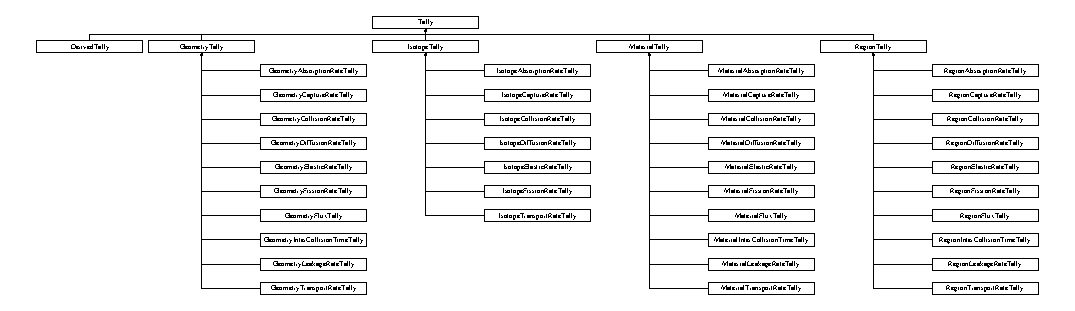
\includegraphics[height=3.733334cm]{classTally}
\end{center}
\end{figure}
\subsection*{Public Member Functions}
\begin{DoxyCompactItemize}
\item 
\hyperlink{classTally_a95563c7f8706efd453c6902b3c6179b1}{Tally} (const char $\ast$tally\-\_\-name=(char $\ast$)\char`\"{}\char`\"{})
\begin{DoxyCompactList}\small\item\em \hyperlink{classTally}{Tally} constructor. \end{DoxyCompactList}\item 
\hypertarget{classTally_a3e6eaab67081636b9112148102eb5899}{virtual \hyperlink{classTally_a3e6eaab67081636b9112148102eb5899}{$\sim$\-Tally} ()}\label{classTally_a3e6eaab67081636b9112148102eb5899}

\begin{DoxyCompactList}\small\item\em \hyperlink{classTally}{Tally} destructor deletes memory for tallies, number of tallies, bin centers and bin edges (if they have been created). \end{DoxyCompactList}\item 
char $\ast$ \hyperlink{classTally_a2f3a42563be7e98933c78c19e52e7c5c}{get\-Tally\-Name} ()
\begin{DoxyCompactList}\small\item\em Returns the name of the tally. \end{DoxyCompactList}\item 
int \hyperlink{classTally_ae518c682a3716d0b3321ae747ef92704}{get\-Num\-Bins} ()
\begin{DoxyCompactList}\small\item\em Returns the number of tally bins. \end{DoxyCompactList}\item 
double $\ast$ \hyperlink{classTally_afb306972b484690ea8898ce314d67d46}{get\-Bin\-Edges} ()
\begin{DoxyCompactList}\small\item\em Returns a double array of bin edge values. \end{DoxyCompactList}\item 
double $\ast$ \hyperlink{classTally_a3a878332f66dc19864b3d5b59ae04f2d}{get\-Bin\-Centers} ()
\begin{DoxyCompactList}\small\item\em Returns a double array of bin center values. \end{DoxyCompactList}\item 
double \hyperlink{classTally_a86b16eda439737ae86631a0b1f803289}{get\-Bin\-Delta} ()
\begin{DoxyCompactList}\small\item\em Returns the delta spacing between bins. N\-O\-T\-E\-: this value is only non-\/zero for E\-Q\-U\-A\-L and L\-O\-G\-A\-R\-I\-T\-H\-M\-I\-C bin types. \end{DoxyCompactList}\item 
double \hyperlink{classTally_a0d1dac1ef54d60773ea11fdc7f1d3307}{get\-Bin\-Delta} (double sample)
\begin{DoxyCompactList}\small\item\em Returns the delta spacing between the bin edges sandwiching a given sample value. \end{DoxyCompactList}\item 
\hyperlink{Tally_8h_ae351518d24ed6463681aeb5c590c975c}{bin\-Spacing\-Type} \hyperlink{classTally_adf407bd073de89237ab6d01036b3ee9f}{get\-Bin\-Spacing\-Type} ()
\begin{DoxyCompactList}\small\item\em Returns the bin spacing type (E\-Q\-U\-A\-L, L\-O\-G\-A\-R\-I\-T\-H\-M\-I\-C, O\-T\-H\-E\-R). \end{DoxyCompactList}\item 
\hyperlink{Tally_8h_a87b950219b1938f2969431f708ad82f4}{tally\-Domain\-Type} \hyperlink{classTally_ab210b0f87c084b590b13015c1cf5c571}{get\-Tally\-Domain\-Type} ()
\begin{DoxyCompactList}\small\item\em Returns the type of tally for these bins (I\-S\-O\-T\-O\-P\-E, M\-A\-T\-E\-R\-I\-A\-L, R\-E\-G\-I\-O\-N). \end{DoxyCompactList}\item 
\hyperlink{Tally_8h_ad9b32b34ff6309e7781de583a9fa3a81}{tally\-Type} \hyperlink{classTally_aa64325bb650b284d06921a446fca69d0}{get\-Tally\-Type} ()
\begin{DoxyCompactList}\small\item\em Returns the type of tally for these bins (F\-L\-U\-X, C\-O\-L\-L\-I\-S\-I\-O\-N\-\_\-\-R\-A\-T\-E, etc). \end{DoxyCompactList}\item 
double $\ast$$\ast$ \hyperlink{classTally_a08a4dc9960b25baaabf20cbdbad99d28}{get\-Tallies} ()
\begin{DoxyCompactList}\small\item\em Returns a double array of the tallies within each bin. \end{DoxyCompactList}\item 
double \hyperlink{classTally_afe131b5f6370aeb82ff4292e9ef3cb70}{get\-Tally} (int bin\-\_\-index, int batch\-\_\-num)
\begin{DoxyCompactList}\small\item\em Returns a specific tally for a specific bin and batch. \end{DoxyCompactList}\item 
double \hyperlink{classTally_aba62d4ef44ad3e929745481224bebec4}{get\-Max\-Tally} ()
\begin{DoxyCompactList}\small\item\em Returns the maximum tally value among all bins and batches. \end{DoxyCompactList}\item 
double \hyperlink{classTally_a39c6b05facabbf65f458f4a3e443d503}{get\-Min\-Tally} ()
\begin{DoxyCompactList}\small\item\em Returns the maximum tally value among all bins and batches. \end{DoxyCompactList}\item 
int \hyperlink{classTally_a35a15ef66832022745bd02a978e6f8d4}{get\-Bin\-Index} (double sample)
\begin{DoxyCompactList}\small\item\em Finds the bin index for a sample in a set of bins. If the samples is outside the bounds of all bins, it returns infinity. \end{DoxyCompactList}\item 
double \hyperlink{classTally_ab926654752702170cb879b76c1660057}{get\-Max\-Mu} ()
\begin{DoxyCompactList}\small\item\em Returns the maximum average tally over batches. \end{DoxyCompactList}\item 
double \hyperlink{classTally_aa62c201b4e1a458e306ebb466b6cb7d2}{get\-Max\-Variance} ()
\begin{DoxyCompactList}\small\item\em Returns the maximum tally variance over batches. \end{DoxyCompactList}\item 
double \hyperlink{classTally_a93d17ce700aeccfc34910d75458fa686}{get\-Max\-Std\-Dev} ()
\begin{DoxyCompactList}\small\item\em Returns the maximum tally standard deviatoin. \end{DoxyCompactList}\item 
double \hyperlink{classTally_a229f351e7dbb2048e52646cc900244e0}{get\-Max\-Rel\-Err} ()
\begin{DoxyCompactList}\small\item\em Returns the maximum tally relative error. \end{DoxyCompactList}\item 
float \hyperlink{classTally_a5afc8471c13e4460ebc9445cf9493bb1}{get\-Trigger\-Precision} ()
\begin{DoxyCompactList}\small\item\em Returns the trigger precision for this tally. \end{DoxyCompactList}\item 
\hyperlink{Tally_8h_a6262444fe2fb14f53ecfa121012410ac}{trigger\-Type} \hyperlink{classTally_a30323691316283d6e664b7d3b7c55abc}{get\-Trigger\-Type} ()
\begin{DoxyCompactList}\small\item\em Returns the precision trigger type (V\-A\-R\-I\-A\-N\-C\-E, S\-T\-A\-N\-D\-A\-R\-D\-\_\-\-D\-E\-V\-I\-A\-T\-I\-O\-N, R\-E\-L\-A\-T\-I\-V\-E\-\_\-\-E\-R\-R\-O\-R, or N\-O\-N\-E). \end{DoxyCompactList}\item 
bool \hyperlink{classTally_aeaf0d3be761283826c41ae989bfb640a}{has\-Computed\-Batch\-Statistics} ()
\begin{DoxyCompactList}\small\item\em Returns whether or not the tally has computed batch statistics. \end{DoxyCompactList}\item 
void \hyperlink{classTally_a967660153e2e1bb72d479e3e0dc79585}{retrieve\-Tally\-Edges} (double $\ast$data, int num\-\_\-bins)
\begin{DoxyCompactList}\small\item\em This method fills an array with the tally bin edges. \end{DoxyCompactList}\item 
void \hyperlink{classTally_a2e4560220839bb22b553913914bb4f5e}{retrieve\-Tally\-Centers} (double $\ast$data, int num\-\_\-bins)
\begin{DoxyCompactList}\small\item\em This method fills an array with the tally bin centers. \end{DoxyCompactList}\item 
void \hyperlink{classTally_aa7963810e95fc7a91af5e007d75538c4}{retrieve\-Tally\-Mu} (double $\ast$data, int num\-\_\-bins)
\begin{DoxyCompactList}\small\item\em This method fills an array with the average tally values. \end{DoxyCompactList}\item 
void \hyperlink{classTally_a0b0b8bd2a624faad629bb3daa30b1567}{retrieve\-Tally\-Variance} (double $\ast$data, int num\-\_\-bins)
\begin{DoxyCompactList}\small\item\em This method fills an array with the tally variances. \end{DoxyCompactList}\item 
void \hyperlink{classTally_a70914083a4264729a9a8b83a5ffc45c2}{retrieve\-Tally\-Std\-Dev} (double $\ast$data, int num\-\_\-bins)
\begin{DoxyCompactList}\small\item\em This method fills an array with the tally standard deviations. \end{DoxyCompactList}\item 
void \hyperlink{classTally_a20b6ef15f6afbe6e1dfe12b19903f01f}{retrieve\-Tally\-Rel\-Err} (double $\ast$data, int num\-\_\-bins)
\begin{DoxyCompactList}\small\item\em This method fills an array with the tally relative errors. \end{DoxyCompactList}\item 
int \hyperlink{classTally_ac0c609996c4294283d402321016ba321}{get\-Num\-Batches} ()
\begin{DoxyCompactList}\small\item\em Returns the number of batches for this tally. \end{DoxyCompactList}\item 
double $\ast$ \hyperlink{classTally_aa54b7f3336fd4c4b38cd01500cccd44d}{get\-Batch\-Mu} ()
\begin{DoxyCompactList}\small\item\em Returns a pointer to an array of tally batch averages if they have been computed. \end{DoxyCompactList}\item 
double $\ast$ \hyperlink{classTally_a7ec325209f919fd12ffbd3f72ccec874}{get\-Batch\-Variance} ()
\begin{DoxyCompactList}\small\item\em Returns a pointer to an array of tally batch variances if they have been computed. \end{DoxyCompactList}\item 
double $\ast$ \hyperlink{classTally_a619bd4bf16cd2b673cbc6db36412e4fb}{get\-Batch\-Std\-Dev} ()
\begin{DoxyCompactList}\small\item\em Returns a pointer to an array of tally batch standard deviations if they have been computed. \end{DoxyCompactList}\item 
double $\ast$ \hyperlink{classTally_a8fccc29c3e4b149a7736cea726695703}{get\-Batch\-Relative\-Error} ()
\begin{DoxyCompactList}\small\item\em Returns a pointer to an array of tally batch relative errors if they have been computed. \end{DoxyCompactList}\item 
void \hyperlink{classTally_a1c4beb9f41a8cf07f397f3b2a08100e3}{set\-Tally\-Domain\-Type} (\hyperlink{Tally_8h_a87b950219b1938f2969431f708ad82f4}{tally\-Domain\-Type} type)
\begin{DoxyCompactList}\small\item\em Set the tally domain type (M\-A\-T\-E\-R\-I\-A\-L, R\-E\-G\-I\-O\-N, etc.). \end{DoxyCompactList}\item 
void \hyperlink{classTally_abd8d1ca36b14ad8d9258ed3f515114f5}{set\-Tally\-Type} (\hyperlink{Tally_8h_ad9b32b34ff6309e7781de583a9fa3a81}{tally\-Type} type)
\begin{DoxyCompactList}\small\item\em Set the tally type (F\-L\-U\-X, C\-A\-P\-T\-U\-R\-E\-\_\-\-R\-A\-T\-E, etc.). \end{DoxyCompactList}\item 
void \hyperlink{classTally_adaa2b02b7ceec6a6d4b7afab3a3948c9}{set\-Bin\-Spacing\-Type} (\hyperlink{Tally_8h_ae351518d24ed6463681aeb5c590c975c}{bin\-Spacing\-Type} type)
\begin{DoxyCompactList}\small\item\em Set the bin spacing type for this \hyperlink{classTally}{Tally} (E\-Q\-U\-A\-L, L\-O\-G\-A\-R\-I\-T\-H\-M\-I\-C, O\-T\-H\-E\-R). \end{DoxyCompactList}\item 
void \hyperlink{classTally_a0552202b4602de16806c5cb100b417ea}{set\-Bin\-Edges} (double $\ast$edges, int num\-\_\-edges)
\begin{DoxyCompactList}\small\item\em Set a user-\/defined double array of bin edge values. \end{DoxyCompactList}\item 
void \hyperlink{classTally_a5284760b90e97c59b7f6cf71a7a36cf8}{set\-Precision\-Trigger} (\hyperlink{Tally_8h_a6262444fe2fb14f53ecfa121012410ac}{trigger\-Type} trigger\-\_\-type, float precision)
\begin{DoxyCompactList}\small\item\em Sets a precision trigger for this tally. \end{DoxyCompactList}\item 
void \hyperlink{classTally_afffe72eb37c973de5841b58ff25f39f8}{generate\-Bin\-Edges} (double start, double end, int num\-\_\-bins, \hyperlink{Tally_8h_ae351518d24ed6463681aeb5c590c975c}{bin\-Spacing\-Type} type)
\begin{DoxyCompactList}\small\item\em Generate edges between bins defined by a start and end point. \end{DoxyCompactList}\item 
void \hyperlink{classTally_af51fb1949401345e6bf1c49ca9081282}{generate\-Bin\-Centers} ()
\begin{DoxyCompactList}\small\item\em Compute the center points between bin edges for this \hyperlink{classTally}{Tally}'s bins. \end{DoxyCompactList}\item 
void \hyperlink{classTally_aa9151ca7c865222b499032af22ab76c8}{set\-Num\-Batches} (int num\-\_\-batches)
\begin{DoxyCompactList}\small\item\em Set the number of batches for this \hyperlink{classTally}{Tally}. \end{DoxyCompactList}\item 
void \hyperlink{classTally_a0c2ee4c8fd57b8b51df52a0abe62ec06}{increment\-Num\-Batches} (int num\-\_\-batches)
\begin{DoxyCompactList}\small\item\em Increments the number of batches for this tally. \end{DoxyCompactList}\item 
bool \hyperlink{classTally_acc38798b21b99da9b1c04bfa4d067547}{is\-Precision\-Triggered} ()
\begin{DoxyCompactList}\small\item\em Returns whether or not the tally precision meets the precision trigger threshold, if a trigger exists. \end{DoxyCompactList}\item 
void \hyperlink{classTally_a2c6ba9c07af18d5b2fda8840791dab14}{compute\-Batch\-Statistics} ()
\begin{DoxyCompactList}\small\item\em Computes average, variance, standard deviation and relative error for each bin over the set of batches. \end{DoxyCompactList}\item 
void \hyperlink{classTally_a7b34a782b04b7056fe7d3ea4b70828e7}{compute\-Scaled\-Batch\-Statistics} (double scale\-\_\-factor)
\begin{DoxyCompactList}\small\item\em Computes average, variance, standard deviation and relative error for each bin over the set of batches. \end{DoxyCompactList}\item 
\hypertarget{classTally_a79fc34d3cb879defffcc9cce4254c36b}{void \hyperlink{classTally_a79fc34d3cb879defffcc9cce4254c36b}{normalize\-Batch\-Mu} ()}\label{classTally_a79fc34d3cb879defffcc9cce4254c36b}

\begin{DoxyCompactList}\small\item\em Divide each tally by the maximum tally value. \end{DoxyCompactList}\item 
void \hyperlink{classTally_a4fd93a5423286a5a9b7953cc8d1dcbcf}{output\-Batch\-Statistics} (const char $\ast$filename)
\begin{DoxyCompactList}\small\item\em Outputs the batch statistics (if they have been computed) to an A\-S\-C\-I\-I file. \end{DoxyCompactList}\item 
void \hyperlink{classTally_a768409c213020f8cb544718c1afce0ea}{print\-Tallies} (bool uncertainties=false)
\begin{DoxyCompactList}\small\item\em Print the tally values to the screen. \end{DoxyCompactList}\item 
\hyperlink{classTally}{Tally} $\ast$ \hyperlink{classTally_a9d96448ef6b56fe491a9b4d5e2d454df}{clone} ()
\begin{DoxyCompactList}\small\item\em Creates a new version of this tally with identical data. \end{DoxyCompactList}\item 
void \hyperlink{classTally_a50c7919393799145f1ab23457d47b02b}{tally} (\hyperlink{structneutron}{neutron} $\ast$\hyperlink{structneutron}{neutron}, double weight)
\begin{DoxyCompactList}\small\item\em This method tallies a particular weight for a neutron. \end{DoxyCompactList}\item 
virtual void \hyperlink{classTally_afb566ef038a61e2449311f2ae95e862e}{tally} (\hyperlink{structneutron}{neutron} $\ast$\hyperlink{structneutron}{neutron})=0
\begin{DoxyCompactList}\small\item\em A virtual method to tally a neutron which must be implemented by \hyperlink{classTally}{Tally} subclasses. \end{DoxyCompactList}\item 
\hyperlink{classDerivedTally}{Derived\-Tally} $\ast$ \hyperlink{classTally_a80264c1e85d8ae1163136097621b48ba}{add\-Integers} (const int $\ast$amt, const int length)
\begin{DoxyCompactList}\small\item\em \hyperlink{classTally}{Tally} addition with an array of integers. \end{DoxyCompactList}\item 
\hyperlink{classDerivedTally}{Derived\-Tally} $\ast$ \hyperlink{classTally_ad23d3e3db6184a558c6bad478084fb49}{add\-Floats} (const float $\ast$amt, const int length)
\begin{DoxyCompactList}\small\item\em \hyperlink{classTally}{Tally} addition with an array of floats. \end{DoxyCompactList}\item 
\hyperlink{classDerivedTally}{Derived\-Tally} $\ast$ \hyperlink{classTally_a21d2d7cbaf3e59c2612abf9f94168cfd}{add\-Doubles} (const double $\ast$amt, const int length)
\begin{DoxyCompactList}\small\item\em \hyperlink{classTally}{Tally} addition with an array of doubles. \end{DoxyCompactList}\item 
\hyperlink{classDerivedTally}{Derived\-Tally} $\ast$ \hyperlink{classTally_aebd2a26ce513bfde74ccbb97bee1635b}{subtract\-Integers} (const int $\ast$amt, const int length)
\begin{DoxyCompactList}\small\item\em \hyperlink{classTally}{Tally} subtraction with an array of integers. \end{DoxyCompactList}\item 
\hyperlink{classDerivedTally}{Derived\-Tally} $\ast$ \hyperlink{classTally_aaafa8791ea206e5da93082081b94abf5}{subtract\-Floats} (const float $\ast$amt, const int length)
\begin{DoxyCompactList}\small\item\em \hyperlink{classTally}{Tally} subtraction with an array of floats. \end{DoxyCompactList}\item 
\hyperlink{classDerivedTally}{Derived\-Tally} $\ast$ \hyperlink{classTally_ad6055bb7f1fc7dc711d6373511be9863}{subtract\-Doubles} (const double $\ast$amt, const int length)
\begin{DoxyCompactList}\small\item\em \hyperlink{classTally}{Tally} subtraction with an array of doubles. \end{DoxyCompactList}\item 
\hyperlink{classDerivedTally}{Derived\-Tally} $\ast$ \hyperlink{classTally_acd3f7c0344ef5878953eec7ff704100e}{multiply\-Integers} (const int $\ast$amt, const int length)
\begin{DoxyCompactList}\small\item\em \hyperlink{classTally}{Tally} multiplication with an array of integers. \end{DoxyCompactList}\item 
\hyperlink{classDerivedTally}{Derived\-Tally} $\ast$ \hyperlink{classTally_a6c65125170bb849a80e1e88fa3c31152}{multiply\-Floats} (const float $\ast$amt, const int length)
\begin{DoxyCompactList}\small\item\em \hyperlink{classTally}{Tally} multiplication with an array of floats. \end{DoxyCompactList}\item 
\hyperlink{classDerivedTally}{Derived\-Tally} $\ast$ \hyperlink{classTally_a1128fb118526992d780449b2cb321b2b}{multiply\-Doubles} (const double $\ast$amt, const int length)
\begin{DoxyCompactList}\small\item\em \hyperlink{classTally}{Tally} multiplication with an array of doubles. \end{DoxyCompactList}\item 
\hyperlink{classDerivedTally}{Derived\-Tally} $\ast$ \hyperlink{classTally_aa5ec92d46f8b27461dd8d92de3fda86e}{divide\-Integers} (const int $\ast$amt, const int length)
\begin{DoxyCompactList}\small\item\em \hyperlink{classTally}{Tally} division with an array of integers. \end{DoxyCompactList}\item 
\hyperlink{classDerivedTally}{Derived\-Tally} $\ast$ \hyperlink{classTally_a76b9fa35eabb07d0e31d994b627983a8}{divide\-Floats} (const float $\ast$amt, const int length)
\begin{DoxyCompactList}\small\item\em \hyperlink{classTally}{Tally} division with an array of floats. \end{DoxyCompactList}\item 
\hyperlink{classDerivedTally}{Derived\-Tally} $\ast$ \hyperlink{classTally_aff77b58ca33931af447b80668e6ea5b7}{divide\-Doubles} (const double $\ast$amt, const int length)
\begin{DoxyCompactList}\small\item\em \hyperlink{classTally}{Tally} division with an array of doubles. \end{DoxyCompactList}\item 
\hyperlink{classDerivedTally}{Derived\-Tally} $\ast$ \hyperlink{classTally_aecaeb26eeb3781184e3bc2d40980d8ea}{operator+} (\hyperlink{classTally}{Tally} $\ast$\hyperlink{classTally_a50c7919393799145f1ab23457d47b02b}{tally})
\begin{DoxyCompactList}\small\item\em \hyperlink{classTally}{Tally} addition operator. \end{DoxyCompactList}\item 
\hyperlink{classDerivedTally}{Derived\-Tally} $\ast$ \hyperlink{classTally_afe9c9e2d762ee9cc2776d4d899d7aa97}{operator-\/} (\hyperlink{classTally}{Tally} $\ast$\hyperlink{classTally_a50c7919393799145f1ab23457d47b02b}{tally})
\begin{DoxyCompactList}\small\item\em \hyperlink{classTally}{Tally} subtraction operator. \end{DoxyCompactList}\item 
\hyperlink{classDerivedTally}{Derived\-Tally} $\ast$ \hyperlink{classTally_a1918c9ad0006fb896c78f5acd93e867a}{operator$\ast$} (\hyperlink{classTally}{Tally} $\ast$\hyperlink{classTally_a50c7919393799145f1ab23457d47b02b}{tally})
\begin{DoxyCompactList}\small\item\em \hyperlink{classTally}{Tally} multiplication operator. \end{DoxyCompactList}\item 
\hyperlink{classDerivedTally}{Derived\-Tally} $\ast$ \hyperlink{classTally_ad43cc4bf0bb3a45b6dd79932b172201b}{operator/} (\hyperlink{classTally}{Tally} $\ast$\hyperlink{classTally_a50c7919393799145f1ab23457d47b02b}{tally})
\begin{DoxyCompactList}\small\item\em \hyperlink{classTally}{Tally} division operator. \end{DoxyCompactList}\item 
\hyperlink{classDerivedTally}{Derived\-Tally} $\ast$ \hyperlink{classTally_a98acdc4cdf80878d8b471d347782e40c}{operator+} (const int amt)
\begin{DoxyCompactList}\small\item\em \hyperlink{classTally}{Tally} addition with a constant operator. \end{DoxyCompactList}\item 
\hyperlink{classDerivedTally}{Derived\-Tally} $\ast$ \hyperlink{classTally_ad54fc16952410ff694caf17e5d133ac4}{operator-\/} (const int amt)
\begin{DoxyCompactList}\small\item\em \hyperlink{classTally}{Tally} subtraction with a constant operator. \end{DoxyCompactList}\item 
\hyperlink{classDerivedTally}{Derived\-Tally} $\ast$ \hyperlink{classTally_a4a495bfff886e894a06f3741ef47b0a2}{operator$\ast$} (const int amt)
\begin{DoxyCompactList}\small\item\em \hyperlink{classTally}{Tally} multiplication with a constant operator. \end{DoxyCompactList}\item 
\hyperlink{classDerivedTally}{Derived\-Tally} $\ast$ \hyperlink{classTally_a8bffb42dbecf2d27335ec82de3fdfa25}{operator/} (const int amt)
\begin{DoxyCompactList}\small\item\em \hyperlink{classTally}{Tally} division with a constant operator. \end{DoxyCompactList}\item 
\hyperlink{classDerivedTally}{Derived\-Tally} $\ast$ \hyperlink{classTally_a6cd03551311465fe6e2b45b0bc69a2c6}{operator+} (const float amt)
\begin{DoxyCompactList}\small\item\em \hyperlink{classTally}{Tally} addition with a constant operator. \end{DoxyCompactList}\item 
\hyperlink{classDerivedTally}{Derived\-Tally} $\ast$ \hyperlink{classTally_a278bfee53b40a392b0b6db258829e755}{operator-\/} (const float amt)
\begin{DoxyCompactList}\small\item\em \hyperlink{classTally}{Tally} subtraction with a constant operator. \end{DoxyCompactList}\item 
\hyperlink{classDerivedTally}{Derived\-Tally} $\ast$ \hyperlink{classTally_a7dba6e707d83273d2f3c94468ff5ed7e}{operator$\ast$} (const float amt)
\begin{DoxyCompactList}\small\item\em \hyperlink{classTally}{Tally} multiplication with a constant operator. \end{DoxyCompactList}\item 
\hyperlink{classDerivedTally}{Derived\-Tally} $\ast$ \hyperlink{classTally_a95b5dbad09760c1ef6887887d6b0da70}{operator/} (const float amt)
\begin{DoxyCompactList}\small\item\em \hyperlink{classTally}{Tally} division with a constant operator. \end{DoxyCompactList}\item 
\hyperlink{classDerivedTally}{Derived\-Tally} $\ast$ \hyperlink{classTally_ae30c13c864d0b983730c21e5ac1c64f8}{operator+} (const double amt)
\begin{DoxyCompactList}\small\item\em \hyperlink{classTally}{Tally} addition with a constant operator. \end{DoxyCompactList}\item 
\hyperlink{classDerivedTally}{Derived\-Tally} $\ast$ \hyperlink{classTally_aa4a6dab9e7ee4d473cf84128a0d042b2}{operator-\/} (const double amt)
\begin{DoxyCompactList}\small\item\em \hyperlink{classTally}{Tally} subtraction with a constant operator. \end{DoxyCompactList}\item 
\hyperlink{classDerivedTally}{Derived\-Tally} $\ast$ \hyperlink{classTally_a05b8241d523d1205317214ec5236a613}{operator$\ast$} (const double amt)
\begin{DoxyCompactList}\small\item\em \hyperlink{classTally}{Tally} multiplication with a constant operator. \end{DoxyCompactList}\item 
\hyperlink{classDerivedTally}{Derived\-Tally} $\ast$ \hyperlink{classTally_ab0a24883876b8ac95fd0c0cb36369aa7}{operator/} (const double amt)
\begin{DoxyCompactList}\small\item\em \hyperlink{classTally}{Tally} division with a constant operator. \end{DoxyCompactList}\end{DoxyCompactItemize}
\subsection*{Protected Attributes}
\begin{DoxyCompactItemize}
\item 
char $\ast$ \hyperlink{classTally_aafa6cfec6391cb1e6247251a6ca7d8ff}{\-\_\-tally\-\_\-name}
\item 
int \hyperlink{classTally_a2f4828eaf5d1de0b4d8aefd7c62171e6}{\-\_\-num\-\_\-bins}
\item 
double $\ast$ \hyperlink{classTally_a2cd7b0c78c22b6ba926f55575a38723c}{\-\_\-edges}
\item 
double $\ast$ \hyperlink{classTally_a7248cac93d9c10a52ad9ce02354b288d}{\-\_\-centers}
\item 
double $\ast$$\ast$ \hyperlink{classTally_ae590e52cd88360d5fb37cc22fe0631d6}{\-\_\-tallies}
\item 
double \hyperlink{classTally_ae86549476a8e7e485fe73dbb3b3be5b1}{\-\_\-bin\-\_\-delta}
\item 
\hyperlink{Tally_8h_ae351518d24ed6463681aeb5c590c975c}{bin\-Spacing\-Type} \hyperlink{classTally_ac0dd7beca80d78fbbd9296bb3fcb0e5e}{\-\_\-bin\-\_\-spacing}
\item 
\hyperlink{Tally_8h_a87b950219b1938f2969431f708ad82f4}{tally\-Domain\-Type} \hyperlink{classTally_af7eb5cc6844eb1081ac5725334d90071}{\-\_\-tally\-\_\-domain}
\item 
\hyperlink{Tally_8h_ad9b32b34ff6309e7781de583a9fa3a81}{tally\-Type} \hyperlink{classTally_afbacc20607dc0b3fd997d9f18da454ac}{\-\_\-tally\-\_\-type}
\item 
\hyperlink{Tally_8h_a6262444fe2fb14f53ecfa121012410ac}{trigger\-Type} \hyperlink{classTally_a93e93ae8e943327d04e4a041c7f4de8c}{\-\_\-trigger\-\_\-type}
\item 
float \hyperlink{classTally_a3c0580f9c5687a77514c9befa61bb22a}{\-\_\-trigger\-\_\-precision}
\item 
int \hyperlink{classTally_ab9e3d1f11d71a62d51872cff0e70051d}{\-\_\-num\-\_\-batches}
\item 
double $\ast$ \hyperlink{classTally_a72b95f77c52db7b5c0447acd77dcb53e}{\-\_\-batch\-\_\-mu}
\item 
double $\ast$ \hyperlink{classTally_aac2dbe707a5ab7576a8cbb76114f1530}{\-\_\-batch\-\_\-variance}
\item 
double $\ast$ \hyperlink{classTally_a178d0ba17341fd2109b62a116805bbd0}{\-\_\-batch\-\_\-std\-\_\-dev}
\item 
double $\ast$ \hyperlink{classTally_a1867b3ec480d667b298c272e475ea027}{\-\_\-batch\-\_\-rel\-\_\-err}
\item 
bool \hyperlink{classTally_a003383fc219cc3b964b19a1508fb2a7f}{\-\_\-computed\-\_\-statistics}
\end{DoxyCompactItemize}


\subsection{Detailed Description}
A \hyperlink{classTally}{Tally} reprsents a set of bins for tallying some quantity. 

This class represents a set of tallies. A set of values define the edges between bins for each tally. This class holds the edges, the centers between bins. It also allows for tallies to be made within each bin.

A set of values define the edges between bins for each tally. This class holds the edges, the centers between bins and the tallies within each bin. The \hyperlink{classTally}{Tally} class knows how to compute batch-\/based statistics for each tally bin. The \hyperlink{classTally}{Tally} class is an abstract class and must be implemented for each specific type of \hyperlink{classTally}{Tally} the developer might wish to define. 

\subsection{Constructor \& Destructor Documentation}
\hypertarget{classTally_a95563c7f8706efd453c6902b3c6179b1}{\index{Tally@{Tally}!Tally@{Tally}}
\index{Tally@{Tally}!Tally@{Tally}}
\subsubsection[{Tally}]{\setlength{\rightskip}{0pt plus 5cm}Tally\-::\-Tally (
\begin{DoxyParamCaption}
\item[{const char $\ast$}]{tally\-\_\-name = {\ttfamily (char$\ast$)\char`\"{}\char`\"{}}}
\end{DoxyParamCaption}
)}}\label{classTally_a95563c7f8706efd453c6902b3c6179b1}


\hyperlink{classTally}{Tally} constructor. 

Assigns a default number of batches (0) and tally bins (0). 

\subsection{Member Function Documentation}
\hypertarget{classTally_a21d2d7cbaf3e59c2612abf9f94168cfd}{\index{Tally@{Tally}!add\-Doubles@{add\-Doubles}}
\index{add\-Doubles@{add\-Doubles}!Tally@{Tally}}
\subsubsection[{add\-Doubles}]{\setlength{\rightskip}{0pt plus 5cm}{\bf Derived\-Tally} $\ast$ Tally\-::add\-Doubles (
\begin{DoxyParamCaption}
\item[{const double $\ast$}]{amt, }
\item[{const int}]{length}
\end{DoxyParamCaption}
)}}\label{classTally_a21d2d7cbaf3e59c2612abf9f94168cfd}


\hyperlink{classTally}{Tally} addition with an array of doubles. 

This overloaded division operator allows the user to add a tally to an array of doubles, if the number of values equals the number of tally bins. This creates a new D\-E\-R\-I\-V\-E\-D type tally, loads it with the sum of the tally bin averages and the array, and updates its batch statistics appropriately. This method is intended to allow for simple tally arithmetic in Python. This method prototype appears to require two operands -\/ the double array and the length of the array -\/ but in Python it only requires the double array as follows\-:


\begin{DoxyCode}
array = numpy.array([1.2, 3.5, 4.7, 8.2], numpy.dtype=float64)
new\_tally = \hyperlink{classTally_a50c7919393799145f1ab23457d47b02b}{tally}.addDoubles(array)
\end{DoxyCode}



\begin{DoxyParams}{Parameters}
{\em amt} & the right operand and the array to add to the tally \\
\hline
{\em length} & the length of the array \\
\hline
\end{DoxyParams}
\begin{DoxyReturn}{Returns}
a D\-E\-R\-I\-V\-E\-D type tally with the tally sum 
\end{DoxyReturn}
\hypertarget{classTally_ad23d3e3db6184a558c6bad478084fb49}{\index{Tally@{Tally}!add\-Floats@{add\-Floats}}
\index{add\-Floats@{add\-Floats}!Tally@{Tally}}
\subsubsection[{add\-Floats}]{\setlength{\rightskip}{0pt plus 5cm}{\bf Derived\-Tally} $\ast$ Tally\-::add\-Floats (
\begin{DoxyParamCaption}
\item[{const float $\ast$}]{amt, }
\item[{const int}]{length}
\end{DoxyParamCaption}
)}}\label{classTally_ad23d3e3db6184a558c6bad478084fb49}


\hyperlink{classTally}{Tally} addition with an array of floats. 

This overloaded division operator allows the user to add a tally by an array of floats, if the number of values equals the number of tally bins. This creates a new D\-E\-R\-I\-V\-E\-D type tally, loads it with the sum of the tally bin averages and the array, and updates its batch statistics appropriately. This method is intended to allow for simple tally arithmetic in Python. This method prototype appears to require two operands -\/ the float array and the length of the array -\/ but in Python it only requires the integer array as follows\-:


\begin{DoxyCode}
array = numpy.array([1.2, 3.5, 4.7, 8.2], numpy.dtype=float32)
new\_tally = \hyperlink{classTally_a50c7919393799145f1ab23457d47b02b}{tally}.addFloats(array)
\end{DoxyCode}



\begin{DoxyParams}{Parameters}
{\em amt} & the right operand and the array to add to the tally \\
\hline
{\em length} & the length of the array \\
\hline
\end{DoxyParams}
\begin{DoxyReturn}{Returns}
a D\-E\-R\-I\-V\-E\-D type tally with the tally sum 
\end{DoxyReturn}
\hypertarget{classTally_a80264c1e85d8ae1163136097621b48ba}{\index{Tally@{Tally}!add\-Integers@{add\-Integers}}
\index{add\-Integers@{add\-Integers}!Tally@{Tally}}
\subsubsection[{add\-Integers}]{\setlength{\rightskip}{0pt plus 5cm}{\bf Derived\-Tally} $\ast$ Tally\-::add\-Integers (
\begin{DoxyParamCaption}
\item[{const int $\ast$}]{amt, }
\item[{const int}]{length}
\end{DoxyParamCaption}
)}}\label{classTally_a80264c1e85d8ae1163136097621b48ba}


\hyperlink{classTally}{Tally} addition with an array of integers. 

This overloaded division operator allows the user to ad a tally by an array of integers, if the number of values equals the number of tally bins. This creates a new D\-E\-R\-I\-V\-E\-D type tally, loads it with the sum of the tally bin averages and the array, and updates its batch statistics appropriately. This method is intended to allow for simple tally arithmetic in Python. This method prototype appears to require two operands -\/ the integer array and the length of the array -\/ but in Python it only requires the integer array as follows\-:


\begin{DoxyCode}
array = numpy.array([1.2, 3.5, 4.7, 8.2])
new\_tally = \hyperlink{classTally_a50c7919393799145f1ab23457d47b02b}{tally}.addIntegers(array)
\end{DoxyCode}



\begin{DoxyParams}{Parameters}
{\em amt} & the right operand and the the array to add to the tally \\
\hline
{\em length} & the length of the array \\
\hline
\end{DoxyParams}
\begin{DoxyReturn}{Returns}
a D\-E\-R\-I\-V\-E\-D type tally with the tally sum 
\end{DoxyReturn}
\hypertarget{classTally_a9d96448ef6b56fe491a9b4d5e2d454df}{\index{Tally@{Tally}!clone@{clone}}
\index{clone@{clone}!Tally@{Tally}}
\subsubsection[{clone}]{\setlength{\rightskip}{0pt plus 5cm}{\bf Tally} $\ast$ Tally\-::clone (
\begin{DoxyParamCaption}
{}
\end{DoxyParamCaption}
)}}\label{classTally_a9d96448ef6b56fe491a9b4d5e2d454df}


Creates a new version of this tally with identical data. 

The clone method makes a deep copy of all of this tally's data and loads it into a new tally class object. \hypertarget{classTally_a2c6ba9c07af18d5b2fda8840791dab14}{\index{Tally@{Tally}!compute\-Batch\-Statistics@{compute\-Batch\-Statistics}}
\index{compute\-Batch\-Statistics@{compute\-Batch\-Statistics}!Tally@{Tally}}
\subsubsection[{compute\-Batch\-Statistics}]{\setlength{\rightskip}{0pt plus 5cm}void Tally\-::compute\-Batch\-Statistics (
\begin{DoxyParamCaption}
{}
\end{DoxyParamCaption}
)}}\label{classTally_a2c6ba9c07af18d5b2fda8840791dab14}


Computes average, variance, standard deviation and relative error for each bin over the set of batches. 

This method populates private class attribute arrays with the batch statistics. \hypertarget{classTally_a7b34a782b04b7056fe7d3ea4b70828e7}{\index{Tally@{Tally}!compute\-Scaled\-Batch\-Statistics@{compute\-Scaled\-Batch\-Statistics}}
\index{compute\-Scaled\-Batch\-Statistics@{compute\-Scaled\-Batch\-Statistics}!Tally@{Tally}}
\subsubsection[{compute\-Scaled\-Batch\-Statistics}]{\setlength{\rightskip}{0pt plus 5cm}void Tally\-::compute\-Scaled\-Batch\-Statistics (
\begin{DoxyParamCaption}
\item[{double}]{scale\-\_\-factor}
\end{DoxyParamCaption}
)}}\label{classTally_a7b34a782b04b7056fe7d3ea4b70828e7}


Computes average, variance, standard deviation and relative error for each bin over the set of batches. 

This method scales each bin value by a scaling factor. 
\begin{DoxyParams}{Parameters}
{\em scale\-\_\-factor} & the factor to scale each bin value by \\
\hline
\end{DoxyParams}
\hypertarget{classTally_aff77b58ca33931af447b80668e6ea5b7}{\index{Tally@{Tally}!divide\-Doubles@{divide\-Doubles}}
\index{divide\-Doubles@{divide\-Doubles}!Tally@{Tally}}
\subsubsection[{divide\-Doubles}]{\setlength{\rightskip}{0pt plus 5cm}{\bf Derived\-Tally} $\ast$ Tally\-::divide\-Doubles (
\begin{DoxyParamCaption}
\item[{const double $\ast$}]{amt, }
\item[{const int}]{length}
\end{DoxyParamCaption}
)}}\label{classTally_aff77b58ca33931af447b80668e6ea5b7}


\hyperlink{classTally}{Tally} division with an array of doubles. 

This overloaded multiplication operator allows the user to divide a tally by an array of doubles, if the number of values equals the number of tally bins. This creates a new D\-E\-R\-I\-V\-E\-D type tally, loads it with the product of the tally bin averages and the array, and updates its batch statistics appropriately. This method is intended to allow for simple tally arithmetic in Python. This method prototype appears to require two operands -\/ the double array and the length of the array -\/ but in Python it only requires the double array as follows\-:


\begin{DoxyCode}
array = numpy.array([1.2, 3.5, 4.7, 8.2], dtype=numpy.float64)
new\_tally = \hyperlink{classTally_a50c7919393799145f1ab23457d47b02b}{tally}.divideDoubles(array)
\end{DoxyCode}



\begin{DoxyParams}{Parameters}
{\em amt} & the right operand and the array to divide the tally by \\
\hline
{\em length} & the length of the array \\
\hline
\end{DoxyParams}
\begin{DoxyReturn}{Returns}
a D\-E\-R\-I\-V\-E\-D type tally with the tally dividend 
\end{DoxyReturn}
\hypertarget{classTally_a76b9fa35eabb07d0e31d994b627983a8}{\index{Tally@{Tally}!divide\-Floats@{divide\-Floats}}
\index{divide\-Floats@{divide\-Floats}!Tally@{Tally}}
\subsubsection[{divide\-Floats}]{\setlength{\rightskip}{0pt plus 5cm}{\bf Derived\-Tally} $\ast$ Tally\-::divide\-Floats (
\begin{DoxyParamCaption}
\item[{const float $\ast$}]{amt, }
\item[{const int}]{length}
\end{DoxyParamCaption}
)}}\label{classTally_a76b9fa35eabb07d0e31d994b627983a8}


\hyperlink{classTally}{Tally} division with an array of floats. 

This overloaded multiplication operator allows the user to divide a tally by an array of floats, if the number of values equals the number of tally bins. This creates a new D\-E\-R\-I\-V\-E\-D type tally, loads it with the product of the tally bin averages and the array, and updates its batch statistics appropriately. This method is intended to allow for simple tally arithmetic in Python. This method prototype appears to require two operands -\/ the float array and the length of the array -\/ but in Python it only requires the float array as follows\-:


\begin{DoxyCode}
array = numpy.array([1.2, 3.5, 4.7, 8.2], dtype=numpy.float32)
new\_tally = \hyperlink{classTally_a50c7919393799145f1ab23457d47b02b}{tally}.divideFloats(array)
\end{DoxyCode}



\begin{DoxyParams}{Parameters}
{\em amt} & the right operand and the array to divide the tally by \\
\hline
{\em length} & the length of the array \\
\hline
\end{DoxyParams}
\begin{DoxyReturn}{Returns}
a D\-E\-R\-I\-V\-E\-D type tally with the tally dividend 
\end{DoxyReturn}
\hypertarget{classTally_aa5ec92d46f8b27461dd8d92de3fda86e}{\index{Tally@{Tally}!divide\-Integers@{divide\-Integers}}
\index{divide\-Integers@{divide\-Integers}!Tally@{Tally}}
\subsubsection[{divide\-Integers}]{\setlength{\rightskip}{0pt plus 5cm}{\bf Derived\-Tally} $\ast$ Tally\-::divide\-Integers (
\begin{DoxyParamCaption}
\item[{const int $\ast$}]{amt, }
\item[{const int}]{length}
\end{DoxyParamCaption}
)}}\label{classTally_aa5ec92d46f8b27461dd8d92de3fda86e}


\hyperlink{classTally}{Tally} division with an array of integers. 

This overloaded multiplication operator allows the user to divide a tally by an array of integers, if the number of values equals the number of tally bins. This creates a new D\-E\-R\-I\-V\-E\-D type tally, loads it with the product of the tally bin averages and the array, and updates its batch statistics appropriately. This method is intended to allow for simple tally arithmetic in Python. This method prototype appears to require two operands -\/ the integer array and the length of the array -\/ but in Python it only requires the integer array as follows\-:


\begin{DoxyCode}
array = numpy.array([1.2, 3.5, 4.7, 8.2], dtype=numpy.int32)
new\_tally = \hyperlink{classTally_a50c7919393799145f1ab23457d47b02b}{tally}.divideIntegers(array)
\end{DoxyCode}



\begin{DoxyParams}{Parameters}
{\em amt} & the right operand and the array to divide the tally by \\
\hline
{\em length} & the length of the array \\
\hline
\end{DoxyParams}
\begin{DoxyReturn}{Returns}
a D\-E\-R\-I\-V\-E\-D type tally with the tally dividend 
\end{DoxyReturn}
\hypertarget{classTally_af51fb1949401345e6bf1c49ca9081282}{\index{Tally@{Tally}!generate\-Bin\-Centers@{generate\-Bin\-Centers}}
\index{generate\-Bin\-Centers@{generate\-Bin\-Centers}!Tally@{Tally}}
\subsubsection[{generate\-Bin\-Centers}]{\setlength{\rightskip}{0pt plus 5cm}void Tally\-::generate\-Bin\-Centers (
\begin{DoxyParamCaption}
{}
\end{DoxyParamCaption}
)}}\label{classTally_af51fb1949401345e6bf1c49ca9081282}


Compute the center points between bin edges for this \hyperlink{classTally}{Tally}'s bins. 

This method populates a private class attribute array with the bin center values. \hypertarget{classTally_afffe72eb37c973de5841b58ff25f39f8}{\index{Tally@{Tally}!generate\-Bin\-Edges@{generate\-Bin\-Edges}}
\index{generate\-Bin\-Edges@{generate\-Bin\-Edges}!Tally@{Tally}}
\subsubsection[{generate\-Bin\-Edges}]{\setlength{\rightskip}{0pt plus 5cm}void Tally\-::generate\-Bin\-Edges (
\begin{DoxyParamCaption}
\item[{double}]{start, }
\item[{double}]{end, }
\item[{int}]{num\-\_\-bins, }
\item[{{\bf bin\-Spacing\-Type}}]{type}
\end{DoxyParamCaption}
)}}\label{classTally_afffe72eb37c973de5841b58ff25f39f8}


Generate edges between bins defined by a start and end point. 


\begin{DoxyParams}{Parameters}
{\em start} & first bin edge value \\
\hline
{\em end} & last bin edge value \\
\hline
{\em num\-\_\-bins} & the number of bins to be created \\
\hline
{\em type} & the type of bins (E\-Q\-U\-A\-L or L\-O\-G\-A\-R\-I\-T\-H\-M\-I\-C) \\
\hline
\end{DoxyParams}
\hypertarget{classTally_aa54b7f3336fd4c4b38cd01500cccd44d}{\index{Tally@{Tally}!get\-Batch\-Mu@{get\-Batch\-Mu}}
\index{get\-Batch\-Mu@{get\-Batch\-Mu}!Tally@{Tally}}
\subsubsection[{get\-Batch\-Mu}]{\setlength{\rightskip}{0pt plus 5cm}double $\ast$ Tally\-::get\-Batch\-Mu (
\begin{DoxyParamCaption}
{}
\end{DoxyParamCaption}
)}}\label{classTally_aa54b7f3336fd4c4b38cd01500cccd44d}


Returns a pointer to an array of tally batch averages if they have been computed. 

\begin{DoxyReturn}{Returns}
a double array of batch averages for each bin 
\end{DoxyReturn}
\hypertarget{classTally_a8fccc29c3e4b149a7736cea726695703}{\index{Tally@{Tally}!get\-Batch\-Relative\-Error@{get\-Batch\-Relative\-Error}}
\index{get\-Batch\-Relative\-Error@{get\-Batch\-Relative\-Error}!Tally@{Tally}}
\subsubsection[{get\-Batch\-Relative\-Error}]{\setlength{\rightskip}{0pt plus 5cm}double $\ast$ Tally\-::get\-Batch\-Relative\-Error (
\begin{DoxyParamCaption}
{}
\end{DoxyParamCaption}
)}}\label{classTally_a8fccc29c3e4b149a7736cea726695703}


Returns a pointer to an array of tally batch relative errors if they have been computed. 

\begin{DoxyReturn}{Returns}
a double array of batch relative errors for each bin 
\end{DoxyReturn}
\hypertarget{classTally_a619bd4bf16cd2b673cbc6db36412e4fb}{\index{Tally@{Tally}!get\-Batch\-Std\-Dev@{get\-Batch\-Std\-Dev}}
\index{get\-Batch\-Std\-Dev@{get\-Batch\-Std\-Dev}!Tally@{Tally}}
\subsubsection[{get\-Batch\-Std\-Dev}]{\setlength{\rightskip}{0pt plus 5cm}double $\ast$ Tally\-::get\-Batch\-Std\-Dev (
\begin{DoxyParamCaption}
{}
\end{DoxyParamCaption}
)}}\label{classTally_a619bd4bf16cd2b673cbc6db36412e4fb}


Returns a pointer to an array of tally batch standard deviations if they have been computed. 

\begin{DoxyReturn}{Returns}
a double array of batch standard deviations for each bin 
\end{DoxyReturn}
\hypertarget{classTally_a7ec325209f919fd12ffbd3f72ccec874}{\index{Tally@{Tally}!get\-Batch\-Variance@{get\-Batch\-Variance}}
\index{get\-Batch\-Variance@{get\-Batch\-Variance}!Tally@{Tally}}
\subsubsection[{get\-Batch\-Variance}]{\setlength{\rightskip}{0pt plus 5cm}double $\ast$ Tally\-::get\-Batch\-Variance (
\begin{DoxyParamCaption}
{}
\end{DoxyParamCaption}
)}}\label{classTally_a7ec325209f919fd12ffbd3f72ccec874}


Returns a pointer to an array of tally batch variances if they have been computed. 

\begin{DoxyReturn}{Returns}
a double array of batch variances for each bin 
\end{DoxyReturn}
\hypertarget{classTally_a3a878332f66dc19864b3d5b59ae04f2d}{\index{Tally@{Tally}!get\-Bin\-Centers@{get\-Bin\-Centers}}
\index{get\-Bin\-Centers@{get\-Bin\-Centers}!Tally@{Tally}}
\subsubsection[{get\-Bin\-Centers}]{\setlength{\rightskip}{0pt plus 5cm}double $\ast$ Tally\-::get\-Bin\-Centers (
\begin{DoxyParamCaption}
{}
\end{DoxyParamCaption}
)}}\label{classTally_a3a878332f66dc19864b3d5b59ae04f2d}


Returns a double array of bin center values. 

\begin{DoxyReturn}{Returns}
array of bin center values 
\end{DoxyReturn}
\hypertarget{classTally_a86b16eda439737ae86631a0b1f803289}{\index{Tally@{Tally}!get\-Bin\-Delta@{get\-Bin\-Delta}}
\index{get\-Bin\-Delta@{get\-Bin\-Delta}!Tally@{Tally}}
\subsubsection[{get\-Bin\-Delta}]{\setlength{\rightskip}{0pt plus 5cm}double Tally\-::get\-Bin\-Delta (
\begin{DoxyParamCaption}
{}
\end{DoxyParamCaption}
)}}\label{classTally_a86b16eda439737ae86631a0b1f803289}


Returns the delta spacing between bins. N\-O\-T\-E\-: this value is only non-\/zero for E\-Q\-U\-A\-L and L\-O\-G\-A\-R\-I\-T\-H\-M\-I\-C bin types. 

\begin{DoxyReturn}{Returns}
the spacing between bins 
\end{DoxyReturn}
\hypertarget{classTally_a0d1dac1ef54d60773ea11fdc7f1d3307}{\index{Tally@{Tally}!get\-Bin\-Delta@{get\-Bin\-Delta}}
\index{get\-Bin\-Delta@{get\-Bin\-Delta}!Tally@{Tally}}
\subsubsection[{get\-Bin\-Delta}]{\setlength{\rightskip}{0pt plus 5cm}double Tally\-::get\-Bin\-Delta (
\begin{DoxyParamCaption}
\item[{double}]{sample}
\end{DoxyParamCaption}
)}}\label{classTally_a0d1dac1ef54d60773ea11fdc7f1d3307}


Returns the delta spacing between the bin edges sandwiching a given sample value. 


\begin{DoxyParams}{Parameters}
{\em sample} & the value of interest \\
\hline
\end{DoxyParams}
\begin{DoxyReturn}{Returns}
the spacing between bin edges 
\end{DoxyReturn}
\hypertarget{classTally_afb306972b484690ea8898ce314d67d46}{\index{Tally@{Tally}!get\-Bin\-Edges@{get\-Bin\-Edges}}
\index{get\-Bin\-Edges@{get\-Bin\-Edges}!Tally@{Tally}}
\subsubsection[{get\-Bin\-Edges}]{\setlength{\rightskip}{0pt plus 5cm}double $\ast$ Tally\-::get\-Bin\-Edges (
\begin{DoxyParamCaption}
{}
\end{DoxyParamCaption}
)}}\label{classTally_afb306972b484690ea8898ce314d67d46}


Returns a double array of bin edge values. 

\begin{DoxyReturn}{Returns}
array of bin edge values 
\end{DoxyReturn}
\hypertarget{classTally_a35a15ef66832022745bd02a978e6f8d4}{\index{Tally@{Tally}!get\-Bin\-Index@{get\-Bin\-Index}}
\index{get\-Bin\-Index@{get\-Bin\-Index}!Tally@{Tally}}
\subsubsection[{get\-Bin\-Index}]{\setlength{\rightskip}{0pt plus 5cm}int Tally\-::get\-Bin\-Index (
\begin{DoxyParamCaption}
\item[{double}]{sample}
\end{DoxyParamCaption}
)\hspace{0.3cm}{\ttfamily [inline]}}}\label{classTally_a35a15ef66832022745bd02a978e6f8d4}


Finds the bin index for a sample in a set of bins. If the samples is outside the bounds of all bins, it returns infinity. 


\begin{DoxyParams}{Parameters}
{\em sample} & the sample value of interest \\
\hline
\end{DoxyParams}
\begin{DoxyReturn}{Returns}
the bin index for the sample 
\end{DoxyReturn}
\hypertarget{classTally_adf407bd073de89237ab6d01036b3ee9f}{\index{Tally@{Tally}!get\-Bin\-Spacing\-Type@{get\-Bin\-Spacing\-Type}}
\index{get\-Bin\-Spacing\-Type@{get\-Bin\-Spacing\-Type}!Tally@{Tally}}
\subsubsection[{get\-Bin\-Spacing\-Type}]{\setlength{\rightskip}{0pt plus 5cm}{\bf bin\-Spacing\-Type} Tally\-::get\-Bin\-Spacing\-Type (
\begin{DoxyParamCaption}
{}
\end{DoxyParamCaption}
)}}\label{classTally_adf407bd073de89237ab6d01036b3ee9f}


Returns the bin spacing type (E\-Q\-U\-A\-L, L\-O\-G\-A\-R\-I\-T\-H\-M\-I\-C, O\-T\-H\-E\-R). 

\begin{DoxyReturn}{Returns}
the bin spacing type 
\end{DoxyReturn}
\hypertarget{classTally_ab926654752702170cb879b76c1660057}{\index{Tally@{Tally}!get\-Max\-Mu@{get\-Max\-Mu}}
\index{get\-Max\-Mu@{get\-Max\-Mu}!Tally@{Tally}}
\subsubsection[{get\-Max\-Mu}]{\setlength{\rightskip}{0pt plus 5cm}double Tally\-::get\-Max\-Mu (
\begin{DoxyParamCaption}
{}
\end{DoxyParamCaption}
)}}\label{classTally_ab926654752702170cb879b76c1660057}


Returns the maximum average tally over batches. 

\begin{DoxyReturn}{Returns}
the maximum average tally 
\end{DoxyReturn}
\hypertarget{classTally_a229f351e7dbb2048e52646cc900244e0}{\index{Tally@{Tally}!get\-Max\-Rel\-Err@{get\-Max\-Rel\-Err}}
\index{get\-Max\-Rel\-Err@{get\-Max\-Rel\-Err}!Tally@{Tally}}
\subsubsection[{get\-Max\-Rel\-Err}]{\setlength{\rightskip}{0pt plus 5cm}double Tally\-::get\-Max\-Rel\-Err (
\begin{DoxyParamCaption}
{}
\end{DoxyParamCaption}
)}}\label{classTally_a229f351e7dbb2048e52646cc900244e0}


Returns the maximum tally relative error. 

\begin{DoxyReturn}{Returns}
the maximum relative error 
\end{DoxyReturn}
\hypertarget{classTally_a93d17ce700aeccfc34910d75458fa686}{\index{Tally@{Tally}!get\-Max\-Std\-Dev@{get\-Max\-Std\-Dev}}
\index{get\-Max\-Std\-Dev@{get\-Max\-Std\-Dev}!Tally@{Tally}}
\subsubsection[{get\-Max\-Std\-Dev}]{\setlength{\rightskip}{0pt plus 5cm}double Tally\-::get\-Max\-Std\-Dev (
\begin{DoxyParamCaption}
{}
\end{DoxyParamCaption}
)}}\label{classTally_a93d17ce700aeccfc34910d75458fa686}


Returns the maximum tally standard deviatoin. 

\begin{DoxyReturn}{Returns}
the maximum standard deviation 
\end{DoxyReturn}
\hypertarget{classTally_aba62d4ef44ad3e929745481224bebec4}{\index{Tally@{Tally}!get\-Max\-Tally@{get\-Max\-Tally}}
\index{get\-Max\-Tally@{get\-Max\-Tally}!Tally@{Tally}}
\subsubsection[{get\-Max\-Tally}]{\setlength{\rightskip}{0pt plus 5cm}double Tally\-::get\-Max\-Tally (
\begin{DoxyParamCaption}
{}
\end{DoxyParamCaption}
)}}\label{classTally_aba62d4ef44ad3e929745481224bebec4}


Returns the maximum tally value among all bins and batches. 

\begin{DoxyReturn}{Returns}
the maximum tally value 
\end{DoxyReturn}
\hypertarget{classTally_aa62c201b4e1a458e306ebb466b6cb7d2}{\index{Tally@{Tally}!get\-Max\-Variance@{get\-Max\-Variance}}
\index{get\-Max\-Variance@{get\-Max\-Variance}!Tally@{Tally}}
\subsubsection[{get\-Max\-Variance}]{\setlength{\rightskip}{0pt plus 5cm}double Tally\-::get\-Max\-Variance (
\begin{DoxyParamCaption}
{}
\end{DoxyParamCaption}
)}}\label{classTally_aa62c201b4e1a458e306ebb466b6cb7d2}


Returns the maximum tally variance over batches. 

\begin{DoxyReturn}{Returns}
the maximum tally variance 
\end{DoxyReturn}
\hypertarget{classTally_a39c6b05facabbf65f458f4a3e443d503}{\index{Tally@{Tally}!get\-Min\-Tally@{get\-Min\-Tally}}
\index{get\-Min\-Tally@{get\-Min\-Tally}!Tally@{Tally}}
\subsubsection[{get\-Min\-Tally}]{\setlength{\rightskip}{0pt plus 5cm}double Tally\-::get\-Min\-Tally (
\begin{DoxyParamCaption}
{}
\end{DoxyParamCaption}
)}}\label{classTally_a39c6b05facabbf65f458f4a3e443d503}


Returns the maximum tally value among all bins and batches. 

\begin{DoxyReturn}{Returns}
the maximum tally value 
\end{DoxyReturn}
\hypertarget{classTally_ac0c609996c4294283d402321016ba321}{\index{Tally@{Tally}!get\-Num\-Batches@{get\-Num\-Batches}}
\index{get\-Num\-Batches@{get\-Num\-Batches}!Tally@{Tally}}
\subsubsection[{get\-Num\-Batches}]{\setlength{\rightskip}{0pt plus 5cm}int Tally\-::get\-Num\-Batches (
\begin{DoxyParamCaption}
{}
\end{DoxyParamCaption}
)}}\label{classTally_ac0c609996c4294283d402321016ba321}


Returns the number of batches for this tally. 

\begin{DoxyReturn}{Returns}
the number of batches 
\end{DoxyReturn}
\hypertarget{classTally_ae518c682a3716d0b3321ae747ef92704}{\index{Tally@{Tally}!get\-Num\-Bins@{get\-Num\-Bins}}
\index{get\-Num\-Bins@{get\-Num\-Bins}!Tally@{Tally}}
\subsubsection[{get\-Num\-Bins}]{\setlength{\rightskip}{0pt plus 5cm}int Tally\-::get\-Num\-Bins (
\begin{DoxyParamCaption}
{}
\end{DoxyParamCaption}
)}}\label{classTally_ae518c682a3716d0b3321ae747ef92704}


Returns the number of tally bins. 

\begin{DoxyReturn}{Returns}
the number of bins 
\end{DoxyReturn}
\hypertarget{classTally_a08a4dc9960b25baaabf20cbdbad99d28}{\index{Tally@{Tally}!get\-Tallies@{get\-Tallies}}
\index{get\-Tallies@{get\-Tallies}!Tally@{Tally}}
\subsubsection[{get\-Tallies}]{\setlength{\rightskip}{0pt plus 5cm}double $\ast$$\ast$ Tally\-::get\-Tallies (
\begin{DoxyParamCaption}
{}
\end{DoxyParamCaption}
)}}\label{classTally_a08a4dc9960b25baaabf20cbdbad99d28}


Returns a double array of the tallies within each bin. 

\begin{DoxyReturn}{Returns}
an array of 
\end{DoxyReturn}
\hypertarget{classTally_afe131b5f6370aeb82ff4292e9ef3cb70}{\index{Tally@{Tally}!get\-Tally@{get\-Tally}}
\index{get\-Tally@{get\-Tally}!Tally@{Tally}}
\subsubsection[{get\-Tally}]{\setlength{\rightskip}{0pt plus 5cm}double Tally\-::get\-Tally (
\begin{DoxyParamCaption}
\item[{int}]{batch\-\_\-num, }
\item[{int}]{bin\-\_\-index}
\end{DoxyParamCaption}
)}}\label{classTally_afe131b5f6370aeb82ff4292e9ef3cb70}


Returns a specific tally for a specific bin and batch. 


\begin{DoxyParams}{Parameters}
{\em batch\-\_\-num} & the batch of interest \\
\hline
{\em bin\-\_\-index} & the index for the bin of interest \\
\hline
\end{DoxyParams}
\begin{DoxyReturn}{Returns}
the tally within that bin 
\end{DoxyReturn}
\hypertarget{classTally_ab210b0f87c084b590b13015c1cf5c571}{\index{Tally@{Tally}!get\-Tally\-Domain\-Type@{get\-Tally\-Domain\-Type}}
\index{get\-Tally\-Domain\-Type@{get\-Tally\-Domain\-Type}!Tally@{Tally}}
\subsubsection[{get\-Tally\-Domain\-Type}]{\setlength{\rightskip}{0pt plus 5cm}{\bf tally\-Domain\-Type} Tally\-::get\-Tally\-Domain\-Type (
\begin{DoxyParamCaption}
{}
\end{DoxyParamCaption}
)}}\label{classTally_ab210b0f87c084b590b13015c1cf5c571}


Returns the type of tally for these bins (I\-S\-O\-T\-O\-P\-E, M\-A\-T\-E\-R\-I\-A\-L, R\-E\-G\-I\-O\-N). 

\begin{DoxyReturn}{Returns}
the tally type 
\end{DoxyReturn}
\hypertarget{classTally_a2f3a42563be7e98933c78c19e52e7c5c}{\index{Tally@{Tally}!get\-Tally\-Name@{get\-Tally\-Name}}
\index{get\-Tally\-Name@{get\-Tally\-Name}!Tally@{Tally}}
\subsubsection[{get\-Tally\-Name}]{\setlength{\rightskip}{0pt plus 5cm}char $\ast$ Tally\-::get\-Tally\-Name (
\begin{DoxyParamCaption}
{}
\end{DoxyParamCaption}
)}}\label{classTally_a2f3a42563be7e98933c78c19e52e7c5c}


Returns the name of the tally. 

\begin{DoxyReturn}{Returns}
the name of the tally 

the \hyperlink{classTally}{Tally}'s name 
\end{DoxyReturn}
\hypertarget{classTally_aa64325bb650b284d06921a446fca69d0}{\index{Tally@{Tally}!get\-Tally\-Type@{get\-Tally\-Type}}
\index{get\-Tally\-Type@{get\-Tally\-Type}!Tally@{Tally}}
\subsubsection[{get\-Tally\-Type}]{\setlength{\rightskip}{0pt plus 5cm}{\bf tally\-Type} Tally\-::get\-Tally\-Type (
\begin{DoxyParamCaption}
{}
\end{DoxyParamCaption}
)}}\label{classTally_aa64325bb650b284d06921a446fca69d0}


Returns the type of tally for these bins (F\-L\-U\-X, C\-O\-L\-L\-I\-S\-I\-O\-N\-\_\-\-R\-A\-T\-E, etc). 

\begin{DoxyReturn}{Returns}
the tally type 
\end{DoxyReturn}
\hypertarget{classTally_a5afc8471c13e4460ebc9445cf9493bb1}{\index{Tally@{Tally}!get\-Trigger\-Precision@{get\-Trigger\-Precision}}
\index{get\-Trigger\-Precision@{get\-Trigger\-Precision}!Tally@{Tally}}
\subsubsection[{get\-Trigger\-Precision}]{\setlength{\rightskip}{0pt plus 5cm}float Tally\-::get\-Trigger\-Precision (
\begin{DoxyParamCaption}
{}
\end{DoxyParamCaption}
)}}\label{classTally_a5afc8471c13e4460ebc9445cf9493bb1}


Returns the trigger precision for this tally. 

The trigger precision is the threshold value which must be met for all of this tally's values before the P\-I\-N\-S\-P\-E\-C simulation will complete. \begin{DoxyReturn}{Returns}
the trigger precision 
\end{DoxyReturn}
\hypertarget{classTally_a30323691316283d6e664b7d3b7c55abc}{\index{Tally@{Tally}!get\-Trigger\-Type@{get\-Trigger\-Type}}
\index{get\-Trigger\-Type@{get\-Trigger\-Type}!Tally@{Tally}}
\subsubsection[{get\-Trigger\-Type}]{\setlength{\rightskip}{0pt plus 5cm}{\bf trigger\-Type} Tally\-::get\-Trigger\-Type (
\begin{DoxyParamCaption}
{}
\end{DoxyParamCaption}
)}}\label{classTally_a30323691316283d6e664b7d3b7c55abc}


Returns the precision trigger type (V\-A\-R\-I\-A\-N\-C\-E, S\-T\-A\-N\-D\-A\-R\-D\-\_\-\-D\-E\-V\-I\-A\-T\-I\-O\-N, R\-E\-L\-A\-T\-I\-V\-E\-\_\-\-E\-R\-R\-O\-R, or N\-O\-N\-E). 

\begin{DoxyReturn}{Returns}
the trigger precision type. 
\end{DoxyReturn}
\hypertarget{classTally_aeaf0d3be761283826c41ae989bfb640a}{\index{Tally@{Tally}!has\-Computed\-Batch\-Statistics@{has\-Computed\-Batch\-Statistics}}
\index{has\-Computed\-Batch\-Statistics@{has\-Computed\-Batch\-Statistics}!Tally@{Tally}}
\subsubsection[{has\-Computed\-Batch\-Statistics}]{\setlength{\rightskip}{0pt plus 5cm}bool Tally\-::has\-Computed\-Batch\-Statistics (
\begin{DoxyParamCaption}
{}
\end{DoxyParamCaption}
)}}\label{classTally_aeaf0d3be761283826c41ae989bfb640a}


Returns whether or not the tally has computed batch statistics. 

\begin{DoxyReturn}{Returns}
true if the tally has computed batch statistics; otherwise false 
\end{DoxyReturn}
\hypertarget{classTally_a0c2ee4c8fd57b8b51df52a0abe62ec06}{\index{Tally@{Tally}!increment\-Num\-Batches@{increment\-Num\-Batches}}
\index{increment\-Num\-Batches@{increment\-Num\-Batches}!Tally@{Tally}}
\subsubsection[{increment\-Num\-Batches}]{\setlength{\rightskip}{0pt plus 5cm}void Tally\-::increment\-Num\-Batches (
\begin{DoxyParamCaption}
\item[{int}]{num\-\_\-batches}
\end{DoxyParamCaption}
)}}\label{classTally_a0c2ee4c8fd57b8b51df52a0abe62ec06}


Increments the number of batches for this tally. 


\begin{DoxyParams}{Parameters}
{\em num\-\_\-batches} & number of batches to add to the total number of batches. \\
\hline
\end{DoxyParams}
\hypertarget{classTally_acc38798b21b99da9b1c04bfa4d067547}{\index{Tally@{Tally}!is\-Precision\-Triggered@{is\-Precision\-Triggered}}
\index{is\-Precision\-Triggered@{is\-Precision\-Triggered}!Tally@{Tally}}
\subsubsection[{is\-Precision\-Triggered}]{\setlength{\rightskip}{0pt plus 5cm}bool Tally\-::is\-Precision\-Triggered (
\begin{DoxyParamCaption}
{}
\end{DoxyParamCaption}
)}}\label{classTally_acc38798b21b99da9b1c04bfa4d067547}


Returns whether or not the tally precision meets the precision trigger threshold, if a trigger exists. 

\begin{DoxyReturn}{Returns}
true if the precision meets the threshold; otherwise false 
\end{DoxyReturn}
\hypertarget{classTally_a1128fb118526992d780449b2cb321b2b}{\index{Tally@{Tally}!multiply\-Doubles@{multiply\-Doubles}}
\index{multiply\-Doubles@{multiply\-Doubles}!Tally@{Tally}}
\subsubsection[{multiply\-Doubles}]{\setlength{\rightskip}{0pt plus 5cm}{\bf Derived\-Tally} $\ast$ Tally\-::multiply\-Doubles (
\begin{DoxyParamCaption}
\item[{const double $\ast$}]{amt, }
\item[{const int}]{length}
\end{DoxyParamCaption}
)}}\label{classTally_a1128fb118526992d780449b2cb321b2b}


\hyperlink{classTally}{Tally} multiplication with an array of doubles. 

This overloaded multiplication operator allows the user to multiply an array of doubles with a tally, if the number of values equals the number of tally bins. This creates a new D\-E\-R\-I\-V\-E\-D type tally, loads it with the product of the tally bin averages and the array, and updates its batch statistics appropriately. This method is intended to allow for simple tally arithmetic in Python. This method prototype appears to require two operands -\/ the double array and the length of the array -\/ but in Python it only requires the double array as follows\-:


\begin{DoxyCode}
array = numpy.array([1.2, 3.5, 4.7, 8.2], dtype=numpy.float64)
new\_tally = \hyperlink{classTally_a50c7919393799145f1ab23457d47b02b}{tally}.multiplyDoubles(array)
\end{DoxyCode}



\begin{DoxyParams}{Parameters}
{\em amt} & the right operand and the array to multiply with the tally \\
\hline
{\em length} & the length of the array \\
\hline
\end{DoxyParams}
\begin{DoxyReturn}{Returns}
a D\-E\-R\-I\-V\-E\-D type tally with the tally product 
\end{DoxyReturn}
\hypertarget{classTally_a6c65125170bb849a80e1e88fa3c31152}{\index{Tally@{Tally}!multiply\-Floats@{multiply\-Floats}}
\index{multiply\-Floats@{multiply\-Floats}!Tally@{Tally}}
\subsubsection[{multiply\-Floats}]{\setlength{\rightskip}{0pt plus 5cm}{\bf Derived\-Tally} $\ast$ Tally\-::multiply\-Floats (
\begin{DoxyParamCaption}
\item[{const float $\ast$}]{amt, }
\item[{const int}]{length}
\end{DoxyParamCaption}
)}}\label{classTally_a6c65125170bb849a80e1e88fa3c31152}


\hyperlink{classTally}{Tally} multiplication with an array of floats. 

This overloaded multiplication operator allows the user to multiply an array of floats with a tally, if the number of values equals the number of tally bins. This creates a new D\-E\-R\-I\-V\-E\-D type tally, loads it with the product of the tally bin averages and the array, and updates its batch statistics appropriately. This method is intended to allow for simple tally arithmetic in Python. This method prototype appears to require two operands -\/ the float array and the length of the array -\/ but in Python it only requires the float array as follows\-:


\begin{DoxyCode}
array = numpy.array([1.2, 3.5, 4.7, 8.2], dtype=numpy.float32)
new\_tally = \hyperlink{classTally_a50c7919393799145f1ab23457d47b02b}{tally}.multiplyFloats(array)
\end{DoxyCode}



\begin{DoxyParams}{Parameters}
{\em amt} & the right operand and the array to multiply with the tally \\
\hline
{\em length} & the length of the array \\
\hline
\end{DoxyParams}
\begin{DoxyReturn}{Returns}
a D\-E\-R\-I\-V\-E\-D type tally with the tally product 
\end{DoxyReturn}
\hypertarget{classTally_acd3f7c0344ef5878953eec7ff704100e}{\index{Tally@{Tally}!multiply\-Integers@{multiply\-Integers}}
\index{multiply\-Integers@{multiply\-Integers}!Tally@{Tally}}
\subsubsection[{multiply\-Integers}]{\setlength{\rightskip}{0pt plus 5cm}{\bf Derived\-Tally} $\ast$ Tally\-::multiply\-Integers (
\begin{DoxyParamCaption}
\item[{const int $\ast$}]{amt, }
\item[{const int}]{length}
\end{DoxyParamCaption}
)}}\label{classTally_acd3f7c0344ef5878953eec7ff704100e}


\hyperlink{classTally}{Tally} multiplication with an array of integers. 

This overloaded multiplication operator allows the user to multiply an array of integers with a tally, if the number of values equals the number of tally bins. This creates a new D\-E\-R\-I\-V\-E\-D type tally, loads it with the product of the tally bin averages and the array, and updates its batch statistics appropriately. This method is intended to allow for simple tally arithmetic in Python. This method prototype appears to require two operands -\/ the integer array and the length of the array -\/ but in Python it only requires the integer array as follows\-:


\begin{DoxyCode}
array = numpy.array([1.2, 3.5, 4.7, 8.2], dtype=numpy.int32)
new\_tally = \hyperlink{classTally_a50c7919393799145f1ab23457d47b02b}{tally}.multiplyIntegers(array)
\end{DoxyCode}



\begin{DoxyParams}{Parameters}
{\em amt} & the right operand and the array to multiply with the tally \\
\hline
{\em length} & the length of the array \\
\hline
\end{DoxyParams}
\begin{DoxyReturn}{Returns}
a D\-E\-R\-I\-V\-E\-D type tally with the tally product 
\end{DoxyReturn}
\hypertarget{classTally_a1918c9ad0006fb896c78f5acd93e867a}{\index{Tally@{Tally}!operator$\ast$@{operator$\ast$}}
\index{operator$\ast$@{operator$\ast$}!Tally@{Tally}}
\subsubsection[{operator$\ast$}]{\setlength{\rightskip}{0pt plus 5cm}{\bf Derived\-Tally} $\ast$ Tally\-::operator$\ast$ (
\begin{DoxyParamCaption}
\item[{{\bf Tally} $\ast$}]{tally}
\end{DoxyParamCaption}
)}}\label{classTally_a1918c9ad0006fb896c78f5acd93e867a}


\hyperlink{classTally}{Tally} multiplication operator. 

This overloaded multiplication operator allows the user to multiply two tallies with each other, if they have the same number of tallies. The creates a new D\-E\-R\-I\-V\-E\-D type tally, loads it with the product of the tally bin averages for the two tally operands, and computes its batch statistics appropriately. This method is intended to allow for simple tally arithmetic in Python.


\begin{DoxyCode}
new\_tally = tally1 * tally2
\end{DoxyCode}


\begin{DoxyReturn}{Returns}
a D\-E\-R\-I\-V\-E\-D type tally with the tally product 
\end{DoxyReturn}
\hypertarget{classTally_a4a495bfff886e894a06f3741ef47b0a2}{\index{Tally@{Tally}!operator$\ast$@{operator$\ast$}}
\index{operator$\ast$@{operator$\ast$}!Tally@{Tally}}
\subsubsection[{operator$\ast$}]{\setlength{\rightskip}{0pt plus 5cm}{\bf Derived\-Tally} $\ast$ Tally\-::operator$\ast$ (
\begin{DoxyParamCaption}
\item[{const int}]{amt}
\end{DoxyParamCaption}
)}}\label{classTally_a4a495bfff886e894a06f3741ef47b0a2}


\hyperlink{classTally}{Tally} multiplication with a constant operator. 

This overloaded subtraction operator allows the user to multiply a constant with a tally. The creates a new D\-E\-R\-I\-V\-E\-D type tally, loads it with the product of the tally bin averages and the constant, and updates its batch statistics appropriately. constant, and updates its batch statistics appropriately. This method is intended to allow for simple tally arithmetic in Python.


\begin{DoxyCode}
new\_tally = \hyperlink{classTally_a50c7919393799145f1ab23457d47b02b}{tally} * int(3)
\end{DoxyCode}



\begin{DoxyParams}{Parameters}
{\em amt} & the right operand and the constant value to multiply the tally by \\
\hline
\end{DoxyParams}
\begin{DoxyReturn}{Returns}
a D\-E\-R\-I\-V\-E\-D type tally with the tally product 
\end{DoxyReturn}
\hypertarget{classTally_a7dba6e707d83273d2f3c94468ff5ed7e}{\index{Tally@{Tally}!operator$\ast$@{operator$\ast$}}
\index{operator$\ast$@{operator$\ast$}!Tally@{Tally}}
\subsubsection[{operator$\ast$}]{\setlength{\rightskip}{0pt plus 5cm}{\bf Derived\-Tally} $\ast$ Tally\-::operator$\ast$ (
\begin{DoxyParamCaption}
\item[{const float}]{amt}
\end{DoxyParamCaption}
)}}\label{classTally_a7dba6e707d83273d2f3c94468ff5ed7e}


\hyperlink{classTally}{Tally} multiplication with a constant operator. 

This overloaded subtraction operator allows the user to multiply a constant with a tally. The creates a new D\-E\-R\-I\-V\-E\-D type tally, loads it with the product of the tally bin averages and the constant, and updates its batch statistics appropriately. This method is intended to allow for simple tally arithmetic in Python.


\begin{DoxyCode}
new\_tally = \hyperlink{classTally_a50c7919393799145f1ab23457d47b02b}{tally} * float(3.5)
\end{DoxyCode}



\begin{DoxyParams}{Parameters}
{\em amt} & the right operand and the constant value to multiply the tally by \\
\hline
\end{DoxyParams}
\begin{DoxyReturn}{Returns}
a D\-E\-R\-I\-V\-E\-D type tally with the tally product 
\end{DoxyReturn}
\hypertarget{classTally_a05b8241d523d1205317214ec5236a613}{\index{Tally@{Tally}!operator$\ast$@{operator$\ast$}}
\index{operator$\ast$@{operator$\ast$}!Tally@{Tally}}
\subsubsection[{operator$\ast$}]{\setlength{\rightskip}{0pt plus 5cm}{\bf Derived\-Tally} $\ast$ Tally\-::operator$\ast$ (
\begin{DoxyParamCaption}
\item[{const double}]{amt}
\end{DoxyParamCaption}
)}}\label{classTally_a05b8241d523d1205317214ec5236a613}


\hyperlink{classTally}{Tally} multiplication with a constant operator. 

This overloaded subtraction operator allows the user to multiply a constant with a tally. The creates a new D\-E\-R\-I\-V\-E\-D type tally, loads it with the product of the tally bin averages and the constant, and updates its batch statistics appropriately. This method is intended to allow for simple tally arithmetic in Python.


\begin{DoxyCode}
new\_tally = \hyperlink{classTally_a50c7919393799145f1ab23457d47b02b}{tally} * double(3.5)
\end{DoxyCode}



\begin{DoxyParams}{Parameters}
{\em amt} & the right operand and the constant value to multiply the tally by \\
\hline
\end{DoxyParams}
\begin{DoxyReturn}{Returns}
a D\-E\-R\-I\-V\-E\-D type tally with the tally product 
\end{DoxyReturn}
\hypertarget{classTally_aecaeb26eeb3781184e3bc2d40980d8ea}{\index{Tally@{Tally}!operator+@{operator+}}
\index{operator+@{operator+}!Tally@{Tally}}
\subsubsection[{operator+}]{\setlength{\rightskip}{0pt plus 5cm}{\bf Derived\-Tally} $\ast$ Tally\-::operator+ (
\begin{DoxyParamCaption}
\item[{{\bf Tally} $\ast$}]{tally}
\end{DoxyParamCaption}
)}}\label{classTally_aecaeb26eeb3781184e3bc2d40980d8ea}


\hyperlink{classTally}{Tally} addition operator. 

This overloaded addition operator allows the user to add two tallies with each other, if they have the same number of tallies. The creates a new D\-E\-R\-I\-V\-E\-D type tally, loads it with the sum of the tally bin averages for the two tally operands, and computes its batch statistics appropriately. This method is intended to allow for simple tally arithmetic in Python. 
\begin{DoxyCode}
new\_tally = tally1 + tally2
\end{DoxyCode}
 
\begin{DoxyParams}{Parameters}
{\em tally} & the right operand in the tally summation \\
\hline
\end{DoxyParams}
\begin{DoxyReturn}{Returns}
a D\-E\-R\-I\-V\-E\-D type tally with the tally sum 
\end{DoxyReturn}
\hypertarget{classTally_a98acdc4cdf80878d8b471d347782e40c}{\index{Tally@{Tally}!operator+@{operator+}}
\index{operator+@{operator+}!Tally@{Tally}}
\subsubsection[{operator+}]{\setlength{\rightskip}{0pt plus 5cm}{\bf Derived\-Tally} $\ast$ Tally\-::operator+ (
\begin{DoxyParamCaption}
\item[{const int}]{amt}
\end{DoxyParamCaption}
)}}\label{classTally_a98acdc4cdf80878d8b471d347782e40c}


\hyperlink{classTally}{Tally} addition with a constant operator. 

This overloaded addition operator allows the user to add a constant to a tally. The creates a new D\-E\-R\-I\-V\-E\-D type tally, loads it with the sum of the tally bin averages and the constant, and updates its batch statistics appropriately. constant, and updates its batch statistics appropriately. This method is intended to allow for simple tally arithmetic in Python.


\begin{DoxyCode}
new\_tally = \hyperlink{classTally_a50c7919393799145f1ab23457d47b02b}{tally} + int(3)
\end{DoxyCode}



\begin{DoxyParams}{Parameters}
{\em amt} & the right operand and the constant value to add to the tally \\
\hline
\end{DoxyParams}
\begin{DoxyReturn}{Returns}
a D\-E\-R\-I\-V\-E\-D type tally with the tally sum 
\end{DoxyReturn}
\hypertarget{classTally_a6cd03551311465fe6e2b45b0bc69a2c6}{\index{Tally@{Tally}!operator+@{operator+}}
\index{operator+@{operator+}!Tally@{Tally}}
\subsubsection[{operator+}]{\setlength{\rightskip}{0pt plus 5cm}{\bf Derived\-Tally} $\ast$ Tally\-::operator+ (
\begin{DoxyParamCaption}
\item[{const float}]{amt}
\end{DoxyParamCaption}
)}}\label{classTally_a6cd03551311465fe6e2b45b0bc69a2c6}


\hyperlink{classTally}{Tally} addition with a constant operator. 

This overloaded addition operator allows the user to add a constant to a tally. The creates a new D\-E\-R\-I\-V\-E\-D type tally, loads it with the sum of the tally bin averages and the constant, and updates its batch statistics appropriately. This method is intended to allow for simple tally arithmetic in Python.


\begin{DoxyCode}
new\_tally = \hyperlink{classTally_a50c7919393799145f1ab23457d47b02b}{tally} + float(3.5)
\end{DoxyCode}



\begin{DoxyParams}{Parameters}
{\em amt} & the right operand and the constant value to add to the tally \\
\hline
\end{DoxyParams}
\begin{DoxyReturn}{Returns}
a D\-E\-R\-I\-V\-E\-D type tally with the tally sum 
\end{DoxyReturn}
\hypertarget{classTally_ae30c13c864d0b983730c21e5ac1c64f8}{\index{Tally@{Tally}!operator+@{operator+}}
\index{operator+@{operator+}!Tally@{Tally}}
\subsubsection[{operator+}]{\setlength{\rightskip}{0pt plus 5cm}{\bf Derived\-Tally} $\ast$ Tally\-::operator+ (
\begin{DoxyParamCaption}
\item[{const double}]{amt}
\end{DoxyParamCaption}
)}}\label{classTally_ae30c13c864d0b983730c21e5ac1c64f8}


\hyperlink{classTally}{Tally} addition with a constant operator. 

This overloaded addition operator allows the user to add a constant to a tally. The creates a new D\-E\-R\-I\-V\-E\-D type tally, loads it with the sum of the tally bin averages and the constant, and updates its batch statistics appropriately. This method is intended to allow for simple tally arithmetic in Python.


\begin{DoxyCode}
new\_tally = \hyperlink{classTally_a50c7919393799145f1ab23457d47b02b}{tally} + double(3.5)
\end{DoxyCode}



\begin{DoxyParams}{Parameters}
{\em amt} & the right operand and the constant value to add to the tally \\
\hline
\end{DoxyParams}
\begin{DoxyReturn}{Returns}
a D\-E\-R\-I\-V\-E\-D type tally with the tally sum 
\end{DoxyReturn}
\hypertarget{classTally_afe9c9e2d762ee9cc2776d4d899d7aa97}{\index{Tally@{Tally}!operator-\/@{operator-\/}}
\index{operator-\/@{operator-\/}!Tally@{Tally}}
\subsubsection[{operator-\/}]{\setlength{\rightskip}{0pt plus 5cm}{\bf Derived\-Tally} $\ast$ Tally\-::operator-\/ (
\begin{DoxyParamCaption}
\item[{{\bf Tally} $\ast$}]{tally}
\end{DoxyParamCaption}
)}}\label{classTally_afe9c9e2d762ee9cc2776d4d899d7aa97}


\hyperlink{classTally}{Tally} subtraction operator. 

This overloaded subtraction operator allows the user to subtract two tallies with each other, if they have the same number of tallies. The creates a new D\-E\-R\-I\-V\-E\-D type tally, loads it with the difference of the tally bin averages for the two tally operands and computes its batch statistics appropriately. This method is intended to allow for simple tally arithmetic in Python.


\begin{DoxyCode}
new\_tally = tally1 - tally2
\end{DoxyCode}



\begin{DoxyParams}{Parameters}
{\em tally} & the right operand in the tally product \\
\hline
\end{DoxyParams}
\begin{DoxyReturn}{Returns}
a D\-E\-R\-I\-V\-E\-D type tally with the tally difference 
\end{DoxyReturn}
\hypertarget{classTally_ad54fc16952410ff694caf17e5d133ac4}{\index{Tally@{Tally}!operator-\/@{operator-\/}}
\index{operator-\/@{operator-\/}!Tally@{Tally}}
\subsubsection[{operator-\/}]{\setlength{\rightskip}{0pt plus 5cm}{\bf Derived\-Tally} $\ast$ Tally\-::operator-\/ (
\begin{DoxyParamCaption}
\item[{const int}]{amt}
\end{DoxyParamCaption}
)}}\label{classTally_ad54fc16952410ff694caf17e5d133ac4}


\hyperlink{classTally}{Tally} subtraction with a constant operator. 

This overloaded subtraction operator allows the user to subtract a constant from a tally. The creates a new D\-E\-R\-I\-V\-E\-D type tally, loads it with the difference of the tally bin averages and the constant, and updates its batch statistics appropriately. constant, and updates its batch statistics appropriately. This method is intended to allow for simple tally arithmetic in Python.


\begin{DoxyCode}
new\_tally = \hyperlink{classTally_a50c7919393799145f1ab23457d47b02b}{tally} - int(3)
\end{DoxyCode}



\begin{DoxyParams}{Parameters}
{\em amt} & the right operand and the constant value to subtract from the tally \\
\hline
\end{DoxyParams}
\begin{DoxyReturn}{Returns}
a D\-E\-R\-I\-V\-E\-D type tally with the tally difference 
\end{DoxyReturn}
\hypertarget{classTally_a278bfee53b40a392b0b6db258829e755}{\index{Tally@{Tally}!operator-\/@{operator-\/}}
\index{operator-\/@{operator-\/}!Tally@{Tally}}
\subsubsection[{operator-\/}]{\setlength{\rightskip}{0pt plus 5cm}{\bf Derived\-Tally} $\ast$ Tally\-::operator-\/ (
\begin{DoxyParamCaption}
\item[{const float}]{amt}
\end{DoxyParamCaption}
)}}\label{classTally_a278bfee53b40a392b0b6db258829e755}


\hyperlink{classTally}{Tally} subtraction with a constant operator. 

This overloaded subtraction operator allows the user to subtract a constant from a tally. The creates a new D\-E\-R\-I\-V\-E\-D type tally, loads it with the difference of the tally bin averages and the constant, and updates its batch statistics appropriately. This method is intended to allow for simple tally arithmetic in Python.


\begin{DoxyCode}
new\_tally = \hyperlink{classTally_a50c7919393799145f1ab23457d47b02b}{tally} - float(3.5)
\end{DoxyCode}



\begin{DoxyParams}{Parameters}
{\em amt} & the right operand and the constant value to subtract from the tally \\
\hline
\end{DoxyParams}
\begin{DoxyReturn}{Returns}
a D\-E\-R\-I\-V\-E\-D type tally with the tally difference 
\end{DoxyReturn}
\hypertarget{classTally_aa4a6dab9e7ee4d473cf84128a0d042b2}{\index{Tally@{Tally}!operator-\/@{operator-\/}}
\index{operator-\/@{operator-\/}!Tally@{Tally}}
\subsubsection[{operator-\/}]{\setlength{\rightskip}{0pt plus 5cm}{\bf Derived\-Tally} $\ast$ Tally\-::operator-\/ (
\begin{DoxyParamCaption}
\item[{const double}]{amt}
\end{DoxyParamCaption}
)}}\label{classTally_aa4a6dab9e7ee4d473cf84128a0d042b2}


\hyperlink{classTally}{Tally} subtraction with a constant operator. 

This overloaded subtraction operator allows the user to subtract a constant from a tally. The creates a new D\-E\-R\-I\-V\-E\-D type tally, loads it with the difference of the tally bin averages and the constant, and updates its batch statistics appropriately. This method is intended to allow for simple tally arithmetic in Python.


\begin{DoxyCode}
new\_tally = \hyperlink{classTally_a50c7919393799145f1ab23457d47b02b}{tally} - double(3.5)
\end{DoxyCode}



\begin{DoxyParams}{Parameters}
{\em amt} & the right operand and the constant value to subtract from the tally \\
\hline
\end{DoxyParams}
\begin{DoxyReturn}{Returns}
a D\-E\-R\-I\-V\-E\-D type tally with the tally difference 
\end{DoxyReturn}
\hypertarget{classTally_ad43cc4bf0bb3a45b6dd79932b172201b}{\index{Tally@{Tally}!operator/@{operator/}}
\index{operator/@{operator/}!Tally@{Tally}}
\subsubsection[{operator/}]{\setlength{\rightskip}{0pt plus 5cm}{\bf Derived\-Tally} $\ast$ Tally\-::operator/ (
\begin{DoxyParamCaption}
\item[{{\bf Tally} $\ast$}]{tally}
\end{DoxyParamCaption}
)}}\label{classTally_ad43cc4bf0bb3a45b6dd79932b172201b}


\hyperlink{classTally}{Tally} division operator. 

This overloaded division operator allows the user to divide two tallies with each other, if they have the same number of tallies. The creates a new D\-E\-R\-I\-V\-E\-D type tally, loads it with the dividend of the tally bin averages for the two tally operands, and computes its batch statistics appropriately. This method is intended to allow for simple tally arithmetic in Python.


\begin{DoxyCode}
new\_tally = tally1 / tally2
\end{DoxyCode}



\begin{DoxyParams}{Parameters}
{\em tally} & the right operand in the tally division \\
\hline
\end{DoxyParams}
\begin{DoxyReturn}{Returns}
a D\-E\-R\-I\-V\-E\-D type tally with the tally division 
\end{DoxyReturn}
\hypertarget{classTally_a8bffb42dbecf2d27335ec82de3fdfa25}{\index{Tally@{Tally}!operator/@{operator/}}
\index{operator/@{operator/}!Tally@{Tally}}
\subsubsection[{operator/}]{\setlength{\rightskip}{0pt plus 5cm}{\bf Derived\-Tally} $\ast$ Tally\-::operator/ (
\begin{DoxyParamCaption}
\item[{const int}]{amt}
\end{DoxyParamCaption}
)}}\label{classTally_a8bffb42dbecf2d27335ec82de3fdfa25}


\hyperlink{classTally}{Tally} division with a constant operator. 

This overloaded division operator allows the user to divide a tally by a constant. The creates a new D\-E\-R\-I\-V\-E\-D type tally, loads it with the dividend of the tally bin averages and the constant, and updates its batch statistics appropriately. This method is intended to allow for simple tally arithmetic in Python.


\begin{DoxyCode}
new\_tally = \hyperlink{classTally_a50c7919393799145f1ab23457d47b02b}{tally} / int(3)
\end{DoxyCode}



\begin{DoxyParams}{Parameters}
{\em amt} & the right operand and the constant value to divide the tally by \\
\hline
\end{DoxyParams}
\begin{DoxyReturn}{Returns}
a D\-E\-R\-I\-V\-E\-D type tally with the tally product 
\end{DoxyReturn}
\hypertarget{classTally_a95b5dbad09760c1ef6887887d6b0da70}{\index{Tally@{Tally}!operator/@{operator/}}
\index{operator/@{operator/}!Tally@{Tally}}
\subsubsection[{operator/}]{\setlength{\rightskip}{0pt plus 5cm}{\bf Derived\-Tally} $\ast$ Tally\-::operator/ (
\begin{DoxyParamCaption}
\item[{const float}]{amt}
\end{DoxyParamCaption}
)}}\label{classTally_a95b5dbad09760c1ef6887887d6b0da70}


\hyperlink{classTally}{Tally} division with a constant operator. 

This overloaded division operator allows the user to divide a tally by a constant. The creates a new D\-E\-R\-I\-V\-E\-D type tally, loads it with the dividend of the tally bin averages and the constant, and updates its batch statistics appropriately. This method is intended to allow for simple tally arithmetic in Python.


\begin{DoxyCode}
new\_tally = \hyperlink{classTally_a50c7919393799145f1ab23457d47b02b}{tally} / float(3.5)
\end{DoxyCode}



\begin{DoxyParams}{Parameters}
{\em amt} & the right operand and the constant value to divide the tally by \\
\hline
\end{DoxyParams}
\begin{DoxyReturn}{Returns}
a D\-E\-R\-I\-V\-E\-D type tally with the tally product 
\end{DoxyReturn}
\hypertarget{classTally_ab0a24883876b8ac95fd0c0cb36369aa7}{\index{Tally@{Tally}!operator/@{operator/}}
\index{operator/@{operator/}!Tally@{Tally}}
\subsubsection[{operator/}]{\setlength{\rightskip}{0pt plus 5cm}{\bf Derived\-Tally} $\ast$ Tally\-::operator/ (
\begin{DoxyParamCaption}
\item[{const double}]{amt}
\end{DoxyParamCaption}
)}}\label{classTally_ab0a24883876b8ac95fd0c0cb36369aa7}


\hyperlink{classTally}{Tally} division with a constant operator. 

This overloaded division operator allows the user to divide a tally by a constant. The creates a new D\-E\-R\-I\-V\-E\-D type tally, loads it with the dividend of the tally bin averages and the constant, and updates its batch statistics appropriately. array, and updates its batch statistics appropriately. This method is intended to allow for simple tally arithmetic in Python.


\begin{DoxyCode}
new\_tally = \hyperlink{classTally_a50c7919393799145f1ab23457d47b02b}{tally} / double(3.5)
\end{DoxyCode}



\begin{DoxyParams}{Parameters}
{\em amt} & the right operand and the constant value to divide the tally by \\
\hline
\end{DoxyParams}
\begin{DoxyReturn}{Returns}
a D\-E\-R\-I\-V\-E\-D type tally with the tally product 
\end{DoxyReturn}
\hypertarget{classTally_a4fd93a5423286a5a9b7953cc8d1dcbcf}{\index{Tally@{Tally}!output\-Batch\-Statistics@{output\-Batch\-Statistics}}
\index{output\-Batch\-Statistics@{output\-Batch\-Statistics}!Tally@{Tally}}
\subsubsection[{output\-Batch\-Statistics}]{\setlength{\rightskip}{0pt plus 5cm}void Tally\-::output\-Batch\-Statistics (
\begin{DoxyParamCaption}
\item[{const char $\ast$}]{filename}
\end{DoxyParamCaption}
)}}\label{classTally_a4fd93a5423286a5a9b7953cc8d1dcbcf}


Outputs the batch statistics (if they have been computed) to an A\-S\-C\-I\-I file. 


\begin{DoxyParams}{Parameters}
{\em filename} & the output filename (optional) \\
\hline
\end{DoxyParams}
\hypertarget{classTally_a768409c213020f8cb544718c1afce0ea}{\index{Tally@{Tally}!print\-Tallies@{print\-Tallies}}
\index{print\-Tallies@{print\-Tallies}!Tally@{Tally}}
\subsubsection[{print\-Tallies}]{\setlength{\rightskip}{0pt plus 5cm}void Tally\-::print\-Tallies (
\begin{DoxyParamCaption}
\item[{bool}]{uncertainties = {\ttfamily false}}
\end{DoxyParamCaption}
)}}\label{classTally_a768409c213020f8cb544718c1afce0ea}


Print the tally values to the screen. 

This method will print the tally results, including bin edges tally averages, and if a user requests, even tally batch statistics. 
\begin{DoxyParams}{Parameters}
{\em uncertainties} & a boolean representing whether or not to print tally statistics \\
\hline
\end{DoxyParams}
\hypertarget{classTally_a2e4560220839bb22b553913914bb4f5e}{\index{Tally@{Tally}!retrieve\-Tally\-Centers@{retrieve\-Tally\-Centers}}
\index{retrieve\-Tally\-Centers@{retrieve\-Tally\-Centers}!Tally@{Tally}}
\subsubsection[{retrieve\-Tally\-Centers}]{\setlength{\rightskip}{0pt plus 5cm}void Tally\-::retrieve\-Tally\-Centers (
\begin{DoxyParamCaption}
\item[{double $\ast$}]{data, }
\item[{int}]{num\-\_\-bins}
\end{DoxyParamCaption}
)}}\label{classTally_a2e4560220839bb22b553913914bb4f5e}


This method fills an array with the tally bin centers. 

This method is a utility function for users to access P\-I\-N\-S\-P\-E\-C data in Python. The method prototype may seem to require two arguments
\begin{DoxyItemize}
\item the array to fill and the number of tally bins -\/ but in Python the user must only supply the data array as follows\-:
\end{DoxyItemize}


\begin{DoxyCode}
num\_bins = \hyperlink{classTally_a50c7919393799145f1ab23457d47b02b}{tally}.getNumBins()
bin\_centers = numpy.zeros(num\_bins)
\hyperlink{classTally_a50c7919393799145f1ab23457d47b02b}{tally}.retrieveTallyCenters(bin\_centers)
\end{DoxyCode}



\begin{DoxyParams}{Parameters}
{\em data} & the data array to fill with bin center values \\
\hline
{\em num\-\_\-bins} & the number of tally bins \\
\hline
\end{DoxyParams}
\hypertarget{classTally_a967660153e2e1bb72d479e3e0dc79585}{\index{Tally@{Tally}!retrieve\-Tally\-Edges@{retrieve\-Tally\-Edges}}
\index{retrieve\-Tally\-Edges@{retrieve\-Tally\-Edges}!Tally@{Tally}}
\subsubsection[{retrieve\-Tally\-Edges}]{\setlength{\rightskip}{0pt plus 5cm}void Tally\-::retrieve\-Tally\-Edges (
\begin{DoxyParamCaption}
\item[{double $\ast$}]{data, }
\item[{int}]{num\-\_\-bins}
\end{DoxyParamCaption}
)}}\label{classTally_a967660153e2e1bb72d479e3e0dc79585}


This method fills an array with the tally bin edges. 

This method is a utility function for users to access P\-I\-N\-S\-P\-E\-C data in Python. The method prototype may seem to require two arguments
\begin{DoxyItemize}
\item the array to fill and the number of tally bins -\/ but in Python the user must only supply the data array as follows\-:
\end{DoxyItemize}


\begin{DoxyCode}
num\_bins = \hyperlink{classTally_a50c7919393799145f1ab23457d47b02b}{tally}.getNumBins()
bin\_edges = numpy.zeros(num\_bins)
\hyperlink{classTally_a50c7919393799145f1ab23457d47b02b}{tally}.retrieveTallyEdges(bin\_edges)
\end{DoxyCode}



\begin{DoxyParams}{Parameters}
{\em data} & the data array to fill with bin edge values \\
\hline
{\em num\-\_\-bins} & the number of tally bins \\
\hline
\end{DoxyParams}
\hypertarget{classTally_aa7963810e95fc7a91af5e007d75538c4}{\index{Tally@{Tally}!retrieve\-Tally\-Mu@{retrieve\-Tally\-Mu}}
\index{retrieve\-Tally\-Mu@{retrieve\-Tally\-Mu}!Tally@{Tally}}
\subsubsection[{retrieve\-Tally\-Mu}]{\setlength{\rightskip}{0pt plus 5cm}void Tally\-::retrieve\-Tally\-Mu (
\begin{DoxyParamCaption}
\item[{double $\ast$}]{data, }
\item[{int}]{num\-\_\-bins}
\end{DoxyParamCaption}
)}}\label{classTally_aa7963810e95fc7a91af5e007d75538c4}


This method fills an array with the average tally values. 

This method is a utility function for users to access P\-I\-N\-S\-P\-E\-C data in Python. The method prototype may seem to require two arguments
\begin{DoxyItemize}
\item the array to fill and the number of tally bins -\/ but in Python the user must only supply the data array as follows\-:
\end{DoxyItemize}


\begin{DoxyCode}
num\_bins = \hyperlink{classTally_a50c7919393799145f1ab23457d47b02b}{tally}.getNumBins()
tally\_averages = numpy.zeros(num\_bins)
\hyperlink{classTally_a50c7919393799145f1ab23457d47b02b}{tally}.retrieveTallyMu(tally\_averages)
\end{DoxyCode}



\begin{DoxyParams}{Parameters}
{\em data} & the data array to fill with tally average values \\
\hline
{\em num\-\_\-bins} & the number of tally bins \\
\hline
\end{DoxyParams}
\hypertarget{classTally_a20b6ef15f6afbe6e1dfe12b19903f01f}{\index{Tally@{Tally}!retrieve\-Tally\-Rel\-Err@{retrieve\-Tally\-Rel\-Err}}
\index{retrieve\-Tally\-Rel\-Err@{retrieve\-Tally\-Rel\-Err}!Tally@{Tally}}
\subsubsection[{retrieve\-Tally\-Rel\-Err}]{\setlength{\rightskip}{0pt plus 5cm}void Tally\-::retrieve\-Tally\-Rel\-Err (
\begin{DoxyParamCaption}
\item[{double $\ast$}]{data, }
\item[{int}]{num\-\_\-bins}
\end{DoxyParamCaption}
)}}\label{classTally_a20b6ef15f6afbe6e1dfe12b19903f01f}


This method fills an array with the tally relative errors. 

This method is a utility function for users to access P\-I\-N\-S\-P\-E\-C data in Python. The method prototype may seem to require two arguments -\/ the array to fill and the number of tally bins -\/ but in Python the user must only supply the data array as follows\-:


\begin{DoxyCode}
num\_bins = \hyperlink{classTally_a50c7919393799145f1ab23457d47b02b}{tally}.getNumBins()
rel\_err = numpy.zeros(num\_bins)
\hyperlink{classTally_a50c7919393799145f1ab23457d47b02b}{tally}.retrieveTallyRelErr(rel\_err)
\end{DoxyCode}



\begin{DoxyParams}{Parameters}
{\em data} & the data array to fill with tally relative errors \\
\hline
{\em num\-\_\-bins} & the number of tally bins \\
\hline
\end{DoxyParams}
\hypertarget{classTally_a70914083a4264729a9a8b83a5ffc45c2}{\index{Tally@{Tally}!retrieve\-Tally\-Std\-Dev@{retrieve\-Tally\-Std\-Dev}}
\index{retrieve\-Tally\-Std\-Dev@{retrieve\-Tally\-Std\-Dev}!Tally@{Tally}}
\subsubsection[{retrieve\-Tally\-Std\-Dev}]{\setlength{\rightskip}{0pt plus 5cm}void Tally\-::retrieve\-Tally\-Std\-Dev (
\begin{DoxyParamCaption}
\item[{double $\ast$}]{data, }
\item[{int}]{num\-\_\-bins}
\end{DoxyParamCaption}
)}}\label{classTally_a70914083a4264729a9a8b83a5ffc45c2}


This method fills an array with the tally standard deviations. 

This method is a utility function for users to access P\-I\-N\-S\-P\-E\-C data in Python. The method prototype may seem to require two arguments -\/ the array to fill and the number of tally bins -\/ but in Python the user must only supply the data array as follows\-:


\begin{DoxyCode}
num\_bins = \hyperlink{classTally_a50c7919393799145f1ab23457d47b02b}{tally}.getNumBins()
std\_dev = numpy.zeros(num\_bins)
\hyperlink{classTally_a50c7919393799145f1ab23457d47b02b}{tally}.retrieveTallyStdDev(std\_dev)
\end{DoxyCode}



\begin{DoxyParams}{Parameters}
{\em data} & the data array to fill with tally standard deviations \\
\hline
{\em num\-\_\-bins} & the number of tally bins \\
\hline
\end{DoxyParams}
\hypertarget{classTally_a0b0b8bd2a624faad629bb3daa30b1567}{\index{Tally@{Tally}!retrieve\-Tally\-Variance@{retrieve\-Tally\-Variance}}
\index{retrieve\-Tally\-Variance@{retrieve\-Tally\-Variance}!Tally@{Tally}}
\subsubsection[{retrieve\-Tally\-Variance}]{\setlength{\rightskip}{0pt plus 5cm}void Tally\-::retrieve\-Tally\-Variance (
\begin{DoxyParamCaption}
\item[{double $\ast$}]{data, }
\item[{int}]{num\-\_\-bins}
\end{DoxyParamCaption}
)}}\label{classTally_a0b0b8bd2a624faad629bb3daa30b1567}


This method fills an array with the tally variances. 

This method is a utility function for users to access P\-I\-N\-S\-P\-E\-C data in Python. The method prototype may seem to require two arguments
\begin{DoxyItemize}
\item the array to fill and the number of tally bins -\/ but in Python the user must only supply the data array as follows\-:
\end{DoxyItemize}


\begin{DoxyCode}
num\_bins = \hyperlink{classTally_a50c7919393799145f1ab23457d47b02b}{tally}.getNumBins()
variances = numpy.zeros(num\_bins)
\hyperlink{classTally_a50c7919393799145f1ab23457d47b02b}{tally}.retrieveTallyVariance(variances)
\end{DoxyCode}



\begin{DoxyParams}{Parameters}
{\em data} & the data array to fill with tally variances \\
\hline
{\em num\-\_\-bins} & the number of tally bins \\
\hline
\end{DoxyParams}
\hypertarget{classTally_a0552202b4602de16806c5cb100b417ea}{\index{Tally@{Tally}!set\-Bin\-Edges@{set\-Bin\-Edges}}
\index{set\-Bin\-Edges@{set\-Bin\-Edges}!Tally@{Tally}}
\subsubsection[{set\-Bin\-Edges}]{\setlength{\rightskip}{0pt plus 5cm}void Tally\-::set\-Bin\-Edges (
\begin{DoxyParamCaption}
\item[{double $\ast$}]{edges, }
\item[{int}]{num\-\_\-edges}
\end{DoxyParamCaption}
)}}\label{classTally_a0552202b4602de16806c5cb100b417ea}


Set a user-\/defined double array of bin edge values. 

This method is intended to allow P\-I\-N\-S\-P\-E\-C users to set tally bin edges through Python. Although this method prototype seems to require two arguments -\/ an array of bin edges and the number of edges -\/ in Python the user only needs to provide the edges array as follows\-:


\begin{DoxyCode}
edges = numpy.array([0.1, 1., 5., 25., 100.])
\hyperlink{classTally_a50c7919393799145f1ab23457d47b02b}{tally}.setBinEdges(edges)
\end{DoxyCode}



\begin{DoxyParams}{Parameters}
{\em edges} & the array of bin edges \\
\hline
{\em num\-\_\-edges} & the number of bin edges \\
\hline
\end{DoxyParams}
\hypertarget{classTally_adaa2b02b7ceec6a6d4b7afab3a3948c9}{\index{Tally@{Tally}!set\-Bin\-Spacing\-Type@{set\-Bin\-Spacing\-Type}}
\index{set\-Bin\-Spacing\-Type@{set\-Bin\-Spacing\-Type}!Tally@{Tally}}
\subsubsection[{set\-Bin\-Spacing\-Type}]{\setlength{\rightskip}{0pt plus 5cm}void Tally\-::set\-Bin\-Spacing\-Type (
\begin{DoxyParamCaption}
\item[{{\bf bin\-Spacing\-Type}}]{type}
\end{DoxyParamCaption}
)}}\label{classTally_adaa2b02b7ceec6a6d4b7afab3a3948c9}


Set the bin spacing type for this \hyperlink{classTally}{Tally} (E\-Q\-U\-A\-L, L\-O\-G\-A\-R\-I\-T\-H\-M\-I\-C, O\-T\-H\-E\-R). 


\begin{DoxyParams}{Parameters}
{\em type} & the bin spacing type \\
\hline
\end{DoxyParams}
\hypertarget{classTally_aa9151ca7c865222b499032af22ab76c8}{\index{Tally@{Tally}!set\-Num\-Batches@{set\-Num\-Batches}}
\index{set\-Num\-Batches@{set\-Num\-Batches}!Tally@{Tally}}
\subsubsection[{set\-Num\-Batches}]{\setlength{\rightskip}{0pt plus 5cm}void Tally\-::set\-Num\-Batches (
\begin{DoxyParamCaption}
\item[{int}]{num\-\_\-batches}
\end{DoxyParamCaption}
)}}\label{classTally_aa9151ca7c865222b499032af22ab76c8}


Set the number of batches for this \hyperlink{classTally}{Tally}. 

This method also allocates memory for the tallies and batch statistics arrays. 
\begin{DoxyParams}{Parameters}
{\em num\-\_\-batches} & the number of batches \\
\hline
\end{DoxyParams}
\hypertarget{classTally_a5284760b90e97c59b7f6cf71a7a36cf8}{\index{Tally@{Tally}!set\-Precision\-Trigger@{set\-Precision\-Trigger}}
\index{set\-Precision\-Trigger@{set\-Precision\-Trigger}!Tally@{Tally}}
\subsubsection[{set\-Precision\-Trigger}]{\setlength{\rightskip}{0pt plus 5cm}void Tally\-::set\-Precision\-Trigger (
\begin{DoxyParamCaption}
\item[{{\bf trigger\-Type}}]{trigger\-\_\-type, }
\item[{float}]{precision}
\end{DoxyParamCaption}
)}}\label{classTally_a5284760b90e97c59b7f6cf71a7a36cf8}


Sets a precision trigger for this tally. 

By setting a precision trigger, the user instructs a P\-I\-N\-S\-E\-P\-C simulation to continue running until all tallies meet the precision trigger threshold. 
\begin{DoxyParams}{Parameters}
{\em trigger\-\_\-type} & the precision trigger type (V\-A\-R\-I\-A\-N\-C\-E, etc) \\
\hline
{\em precision} & the threshold for the precision trigger \\
\hline
\end{DoxyParams}
\hypertarget{classTally_a1c4beb9f41a8cf07f397f3b2a08100e3}{\index{Tally@{Tally}!set\-Tally\-Domain\-Type@{set\-Tally\-Domain\-Type}}
\index{set\-Tally\-Domain\-Type@{set\-Tally\-Domain\-Type}!Tally@{Tally}}
\subsubsection[{set\-Tally\-Domain\-Type}]{\setlength{\rightskip}{0pt plus 5cm}void Tally\-::set\-Tally\-Domain\-Type (
\begin{DoxyParamCaption}
\item[{{\bf tally\-Domain\-Type}}]{type}
\end{DoxyParamCaption}
)}}\label{classTally_a1c4beb9f41a8cf07f397f3b2a08100e3}


Set the tally domain type (M\-A\-T\-E\-R\-I\-A\-L, R\-E\-G\-I\-O\-N, etc.). 


\begin{DoxyParams}{Parameters}
{\em type} & the tally domain type \\
\hline
\end{DoxyParams}
\hypertarget{classTally_abd8d1ca36b14ad8d9258ed3f515114f5}{\index{Tally@{Tally}!set\-Tally\-Type@{set\-Tally\-Type}}
\index{set\-Tally\-Type@{set\-Tally\-Type}!Tally@{Tally}}
\subsubsection[{set\-Tally\-Type}]{\setlength{\rightskip}{0pt plus 5cm}void Tally\-::set\-Tally\-Type (
\begin{DoxyParamCaption}
\item[{{\bf tally\-Type}}]{type}
\end{DoxyParamCaption}
)}}\label{classTally_abd8d1ca36b14ad8d9258ed3f515114f5}


Set the tally type (F\-L\-U\-X, C\-A\-P\-T\-U\-R\-E\-\_\-\-R\-A\-T\-E, etc.). 


\begin{DoxyParams}{Parameters}
{\em type} & the tally type \\
\hline
\end{DoxyParams}
\hypertarget{classTally_ad6055bb7f1fc7dc711d6373511be9863}{\index{Tally@{Tally}!subtract\-Doubles@{subtract\-Doubles}}
\index{subtract\-Doubles@{subtract\-Doubles}!Tally@{Tally}}
\subsubsection[{subtract\-Doubles}]{\setlength{\rightskip}{0pt plus 5cm}{\bf Derived\-Tally} $\ast$ Tally\-::subtract\-Doubles (
\begin{DoxyParamCaption}
\item[{const double $\ast$}]{amt, }
\item[{const int}]{length}
\end{DoxyParamCaption}
)}}\label{classTally_ad6055bb7f1fc7dc711d6373511be9863}


\hyperlink{classTally}{Tally} subtraction with an array of doubles. 

This overloaded subtraction operator allows the user to subtract an array of doubles from a tally, if the number of values equals the number of tally bins. This creates a new D\-E\-R\-I\-V\-E\-D type tally, loads it with the difference of the tally bin averages and the array, and updates its batch statistics appropriately. This method is intended to allow for simple tally arithmetic in Python. This method prototype appears to require two operands -\/ the double array and the length of the array -\/ but in Python it only requires the double array as follows\-:


\begin{DoxyCode}
array = numpy.array([1.2, 3.5, 4.7, 8.2], dtype=numpy.float64)
new\_tally = \hyperlink{classTally_a50c7919393799145f1ab23457d47b02b}{tally}.subtractIntegers(array)
\end{DoxyCode}



\begin{DoxyParams}{Parameters}
{\em amt} & the right operand and the array to subtract from the tally \\
\hline
{\em length} & the length of the array \\
\hline
\end{DoxyParams}
\begin{DoxyReturn}{Returns}
a D\-E\-R\-I\-V\-E\-D type tally with the tally difference 
\end{DoxyReturn}
\hypertarget{classTally_aaafa8791ea206e5da93082081b94abf5}{\index{Tally@{Tally}!subtract\-Floats@{subtract\-Floats}}
\index{subtract\-Floats@{subtract\-Floats}!Tally@{Tally}}
\subsubsection[{subtract\-Floats}]{\setlength{\rightskip}{0pt plus 5cm}{\bf Derived\-Tally} $\ast$ Tally\-::subtract\-Floats (
\begin{DoxyParamCaption}
\item[{const float $\ast$}]{amt, }
\item[{const int}]{length}
\end{DoxyParamCaption}
)}}\label{classTally_aaafa8791ea206e5da93082081b94abf5}


\hyperlink{classTally}{Tally} subtraction with an array of floats. 

This overloaded subtraction operator allows the user to subtract an array of floats from a tally, if the number of values equals the number of tally bins. This creates a new D\-E\-R\-I\-V\-E\-D type tally, loads it with the difference of the tally bin averages and the array, and updates its batch statistics appropriately. This method is intended to allow for simple tally arithmetic in Python. This method prototype appears to require two operands -\/ the float array and the length of the array -\/ but in Python it only requires the float array as follows\-:


\begin{DoxyCode}
array = numpy.array([1.2, 3.5, 4.7, 8.2], dtype=numpy.float32)
new\_tally = \hyperlink{classTally_a50c7919393799145f1ab23457d47b02b}{tally}.subtractFloats(array)
\end{DoxyCode}



\begin{DoxyParams}{Parameters}
{\em amt} & the right operand and the array to subtract from the tally \\
\hline
{\em length} & the length of the array \\
\hline
\end{DoxyParams}
\begin{DoxyReturn}{Returns}
a D\-E\-R\-I\-V\-E\-D type tally with the tally difference 
\end{DoxyReturn}
\hypertarget{classTally_aebd2a26ce513bfde74ccbb97bee1635b}{\index{Tally@{Tally}!subtract\-Integers@{subtract\-Integers}}
\index{subtract\-Integers@{subtract\-Integers}!Tally@{Tally}}
\subsubsection[{subtract\-Integers}]{\setlength{\rightskip}{0pt plus 5cm}{\bf Derived\-Tally} $\ast$ Tally\-::subtract\-Integers (
\begin{DoxyParamCaption}
\item[{const int $\ast$}]{amt, }
\item[{const int}]{length}
\end{DoxyParamCaption}
)}}\label{classTally_aebd2a26ce513bfde74ccbb97bee1635b}


\hyperlink{classTally}{Tally} subtraction with an array of integers. 

This overloaded subtraction operator allows the user to subtract an array of integers from a tally, if the number of values equals the number of tally bins. This creates a new D\-E\-R\-I\-V\-E\-D type tally, loads it with the difference of the tally bin averages and the array, and updates its batch statistics appropriately. This method is intended to allow for simple tally arithmetic in Python. This method prototype appears to require two operands -\/ the integer array and the length of the array -\/ but in Python it only requires the integer array as follows\-:


\begin{DoxyCode}
array = numpy.array([1.2, 3.5, 4.7, 8.2], dtype=numpy.integer)
new\_tally = \hyperlink{classTally_a50c7919393799145f1ab23457d47b02b}{tally}.subtractIntegers(array)
\end{DoxyCode}



\begin{DoxyParams}{Parameters}
{\em amt} & the right operand and the array to subtract from the tally \\
\hline
{\em length} & the length of the array \\
\hline
\end{DoxyParams}
\begin{DoxyReturn}{Returns}
a D\-E\-R\-I\-V\-E\-D type tally with the tally difference 
\end{DoxyReturn}
\hypertarget{classTally_a50c7919393799145f1ab23457d47b02b}{\index{Tally@{Tally}!tally@{tally}}
\index{tally@{tally}!Tally@{Tally}}
\subsubsection[{tally}]{\setlength{\rightskip}{0pt plus 5cm}void Tally\-::tally (
\begin{DoxyParamCaption}
\item[{{\bf neutron} $\ast$}]{neutron, }
\item[{double}]{weight}
\end{DoxyParamCaption}
)}}\label{classTally_a50c7919393799145f1ab23457d47b02b}


This method tallies a particular weight for a neutron. 

The method determines which tally bin to use based on the neutron's energy. 
\begin{DoxyParams}{Parameters}
{\em neutron} & the neutron we are tallying \\
\hline
{\em weight} & the weight to increment tally by \\
\hline
\end{DoxyParams}
\hypertarget{classTally_afb566ef038a61e2449311f2ae95e862e}{\index{Tally@{Tally}!tally@{tally}}
\index{tally@{tally}!Tally@{Tally}}
\subsubsection[{tally}]{\setlength{\rightskip}{0pt plus 5cm}virtual void Tally\-::tally (
\begin{DoxyParamCaption}
\item[{{\bf neutron} $\ast$}]{neutron}
\end{DoxyParamCaption}
)\hspace{0.3cm}{\ttfamily [pure virtual]}}}\label{classTally_afb566ef038a61e2449311f2ae95e862e}


A virtual method to tally a neutron which must be implemented by \hyperlink{classTally}{Tally} subclasses. 


\begin{DoxyParams}{Parameters}
{\em neutron} & the neutron of interest \\
\hline
\end{DoxyParams}


Implemented in \hyperlink{classDerivedTally_a80e9a372015c142cdc74d38b7f281166}{Derived\-Tally}, \hyperlink{classGeometryInterCollisionTimeTally_a8190817fa635809c6ae1bdadd9665ef8}{Geometry\-Inter\-Collision\-Time\-Tally}, \hyperlink{classRegionInterCollisionTimeTally_a389dd158a3a10b959fa444d12a8cb752}{Region\-Inter\-Collision\-Time\-Tally}, \hyperlink{classMaterialInterCollisionTimeTally_a339ebb3a0367954d650006acc72185b9}{Material\-Inter\-Collision\-Time\-Tally}, \hyperlink{classGeometryFluxTally_a2c7d83a4577cff56a1cecf8a339db547}{Geometry\-Flux\-Tally}, \hyperlink{classRegionFluxTally_a318a32edcb4f2866574194cd74ddd04f}{Region\-Flux\-Tally}, \hyperlink{classMaterialFluxTally_a458d77b55dbd6bd0fb5efeb2ffec2e9b}{Material\-Flux\-Tally}, \hyperlink{classGeometryLeakageRateTally_a19498479ed8c16606515fa47bf45a726}{Geometry\-Leakage\-Rate\-Tally}, \hyperlink{classRegionLeakageRateTally_a9f8749a387783d68de8fc8ecaf347748}{Region\-Leakage\-Rate\-Tally}, \hyperlink{classMaterialLeakageRateTally_ad23d9da8c90ce281205d70c3b3132cc3}{Material\-Leakage\-Rate\-Tally}, \hyperlink{classGeometryDiffusionRateTally_aab31c320a689adb46c888bd68df49ad4}{Geometry\-Diffusion\-Rate\-Tally}, \hyperlink{classRegionDiffusionRateTally_a0c581304fc724c57632ed00b5f2e5e0f}{Region\-Diffusion\-Rate\-Tally}, \hyperlink{classMaterialDiffusionRateTally_a63bd04bab0e138059384e35d925a5ce0}{Material\-Diffusion\-Rate\-Tally}, \hyperlink{classIsotopeDiffusionRateTally_af9de72dec40388388faba7fdf13ec5a4}{Isotope\-Diffusion\-Rate\-Tally}, \hyperlink{classGeometryTransportRateTally_ab634a607b837e7e4a8637af0d7ab5d74}{Geometry\-Transport\-Rate\-Tally}, \hyperlink{classRegionTransportRateTally_af373747c50c56011383dcf569a685af2}{Region\-Transport\-Rate\-Tally}, \hyperlink{classMaterialTransportRateTally_a10c3aa96348177a1002395295d51c90a}{Material\-Transport\-Rate\-Tally}, \hyperlink{classIsotopeTransportRateTally_a5a747ab9d3704757ff9ec585fa402e84}{Isotope\-Transport\-Rate\-Tally}, \hyperlink{classGeometryFissionRateTally_aabf84c492a081ac3fb86993be3896a62}{Geometry\-Fission\-Rate\-Tally}, \hyperlink{classRegionFissionRateTally_a1d6e8da254f83a462de8ccf5226f1fee}{Region\-Fission\-Rate\-Tally}, \hyperlink{classMaterialFissionRateTally_aa47cb28d567ce9315872fff4251dce31}{Material\-Fission\-Rate\-Tally}, \hyperlink{classIsotopeFissionRateTally_aeeed9917e1134a1a37ed58a5f94dd569}{Isotope\-Fission\-Rate\-Tally}, \hyperlink{classGeometryCaptureRateTally_a18b5cb68008c52ab416ee7f5b73ac2a5}{Geometry\-Capture\-Rate\-Tally}, \hyperlink{classRegionCaptureRateTally_a200bb4afe0bdf5520cc9756f644ebcd3}{Region\-Capture\-Rate\-Tally}, \hyperlink{classMaterialCaptureRateTally_a786889f9b19e47868b05b065920283e6}{Material\-Capture\-Rate\-Tally}, \hyperlink{classIsotopeCaptureRateTally_a6fb691f21aefd869d86622f6304c05e3}{Isotope\-Capture\-Rate\-Tally}, \hyperlink{classGeometryAbsorptionRateTally_a51490d9c5ee4a9d0447b6722a65fef1a}{Geometry\-Absorption\-Rate\-Tally}, \hyperlink{classRegionAbsorptionRateTally_ac4b4c57159d65550e1e67dfb2037fd09}{Region\-Absorption\-Rate\-Tally}, \hyperlink{classMaterialAbsorptionRateTally_a86c4e2653f1baf2b862ce9d3043a888e}{Material\-Absorption\-Rate\-Tally}, \hyperlink{classIsotopeAbsorptionRateTally_a300abb8c8532c790d514700ed2b5e1ee}{Isotope\-Absorption\-Rate\-Tally}, \hyperlink{classGeometryElasticRateTally_a7bf2a8bc3afbc47354bad45159237ec3}{Geometry\-Elastic\-Rate\-Tally}, \hyperlink{classRegionElasticRateTally_aaafa18c6ed2d9d2da1437cb1d969fa29}{Region\-Elastic\-Rate\-Tally}, \hyperlink{classMaterialElasticRateTally_a8d3104a906c10b34c236275f65aa610d}{Material\-Elastic\-Rate\-Tally}, \hyperlink{classIsotopeElasticRateTally_a641673a78be89eec1f1be4d424f0e078}{Isotope\-Elastic\-Rate\-Tally}, \hyperlink{classGeometryCollisionRateTally_af0b0c1c09c8dbdc5453feb8366600dc0}{Geometry\-Collision\-Rate\-Tally}, \hyperlink{classRegionCollisionRateTally_af365f111715d80311047029fe2e64ce7}{Region\-Collision\-Rate\-Tally}, \hyperlink{classMaterialCollisionRateTally_a3da8ad061bf2b1501a4f6a191ad5dfd9}{Material\-Collision\-Rate\-Tally}, \hyperlink{classIsotopeCollisionRateTally_acd866aa174db9df4b5bdba6347735886}{Isotope\-Collision\-Rate\-Tally}, \hyperlink{classGeometryTally_a3f79423e0c1e1eb87109c6937bdfa5c8}{Geometry\-Tally}, \hyperlink{classRegionTally_ae146fd937e34306fdd5cc4aac44a3856}{Region\-Tally}, \hyperlink{classMaterialTally_ab2debba62f51212ec8b39b7aeea3f54d}{Material\-Tally}, and \hyperlink{classIsotopeTally_a8a5b190e244c630ee7cda35f70287530}{Isotope\-Tally}.



\subsection{Member Data Documentation}
\hypertarget{classTally_a72b95f77c52db7b5c0447acd77dcb53e}{\index{Tally@{Tally}!\-\_\-batch\-\_\-mu@{\-\_\-batch\-\_\-mu}}
\index{\-\_\-batch\-\_\-mu@{\-\_\-batch\-\_\-mu}!Tally@{Tally}}
\subsubsection[{\-\_\-batch\-\_\-mu}]{\setlength{\rightskip}{0pt plus 5cm}double$\ast$ Tally\-::\-\_\-batch\-\_\-mu\hspace{0.3cm}{\ttfamily [protected]}}}\label{classTally_a72b95f77c52db7b5c0447acd77dcb53e}
The batch average for each tally bin \hypertarget{classTally_a1867b3ec480d667b298c272e475ea027}{\index{Tally@{Tally}!\-\_\-batch\-\_\-rel\-\_\-err@{\-\_\-batch\-\_\-rel\-\_\-err}}
\index{\-\_\-batch\-\_\-rel\-\_\-err@{\-\_\-batch\-\_\-rel\-\_\-err}!Tally@{Tally}}
\subsubsection[{\-\_\-batch\-\_\-rel\-\_\-err}]{\setlength{\rightskip}{0pt plus 5cm}double$\ast$ Tally\-::\-\_\-batch\-\_\-rel\-\_\-err\hspace{0.3cm}{\ttfamily [protected]}}}\label{classTally_a1867b3ec480d667b298c272e475ea027}
The batch relative error for each tally bin \hypertarget{classTally_a178d0ba17341fd2109b62a116805bbd0}{\index{Tally@{Tally}!\-\_\-batch\-\_\-std\-\_\-dev@{\-\_\-batch\-\_\-std\-\_\-dev}}
\index{\-\_\-batch\-\_\-std\-\_\-dev@{\-\_\-batch\-\_\-std\-\_\-dev}!Tally@{Tally}}
\subsubsection[{\-\_\-batch\-\_\-std\-\_\-dev}]{\setlength{\rightskip}{0pt plus 5cm}double$\ast$ Tally\-::\-\_\-batch\-\_\-std\-\_\-dev\hspace{0.3cm}{\ttfamily [protected]}}}\label{classTally_a178d0ba17341fd2109b62a116805bbd0}
The batch standard deviation for each tally bin \hypertarget{classTally_aac2dbe707a5ab7576a8cbb76114f1530}{\index{Tally@{Tally}!\-\_\-batch\-\_\-variance@{\-\_\-batch\-\_\-variance}}
\index{\-\_\-batch\-\_\-variance@{\-\_\-batch\-\_\-variance}!Tally@{Tally}}
\subsubsection[{\-\_\-batch\-\_\-variance}]{\setlength{\rightskip}{0pt plus 5cm}double$\ast$ Tally\-::\-\_\-batch\-\_\-variance\hspace{0.3cm}{\ttfamily [protected]}}}\label{classTally_aac2dbe707a5ab7576a8cbb76114f1530}
The batch variance for each tally bin \hypertarget{classTally_ae86549476a8e7e485fe73dbb3b3be5b1}{\index{Tally@{Tally}!\-\_\-bin\-\_\-delta@{\-\_\-bin\-\_\-delta}}
\index{\-\_\-bin\-\_\-delta@{\-\_\-bin\-\_\-delta}!Tally@{Tally}}
\subsubsection[{\-\_\-bin\-\_\-delta}]{\setlength{\rightskip}{0pt plus 5cm}double Tally\-::\-\_\-bin\-\_\-delta\hspace{0.3cm}{\ttfamily [protected]}}}\label{classTally_ae86549476a8e7e485fe73dbb3b3be5b1}
Equal / logarithmic spacing between bins if defined on a uniform grid \hypertarget{classTally_ac0dd7beca80d78fbbd9296bb3fcb0e5e}{\index{Tally@{Tally}!\-\_\-bin\-\_\-spacing@{\-\_\-bin\-\_\-spacing}}
\index{\-\_\-bin\-\_\-spacing@{\-\_\-bin\-\_\-spacing}!Tally@{Tally}}
\subsubsection[{\-\_\-bin\-\_\-spacing}]{\setlength{\rightskip}{0pt plus 5cm}{\bf bin\-Spacing\-Type} Tally\-::\-\_\-bin\-\_\-spacing\hspace{0.3cm}{\ttfamily [protected]}}}\label{classTally_ac0dd7beca80d78fbbd9296bb3fcb0e5e}
The spacing type between bins \hypertarget{classTally_a7248cac93d9c10a52ad9ce02354b288d}{\index{Tally@{Tally}!\-\_\-centers@{\-\_\-centers}}
\index{\-\_\-centers@{\-\_\-centers}!Tally@{Tally}}
\subsubsection[{\-\_\-centers}]{\setlength{\rightskip}{0pt plus 5cm}double$\ast$ Tally\-::\-\_\-centers\hspace{0.3cm}{\ttfamily [protected]}}}\label{classTally_a7248cac93d9c10a52ad9ce02354b288d}
The array of bin center values \hypertarget{classTally_a003383fc219cc3b964b19a1508fb2a7f}{\index{Tally@{Tally}!\-\_\-computed\-\_\-statistics@{\-\_\-computed\-\_\-statistics}}
\index{\-\_\-computed\-\_\-statistics@{\-\_\-computed\-\_\-statistics}!Tally@{Tally}}
\subsubsection[{\-\_\-computed\-\_\-statistics}]{\setlength{\rightskip}{0pt plus 5cm}bool Tally\-::\-\_\-computed\-\_\-statistics\hspace{0.3cm}{\ttfamily [protected]}}}\label{classTally_a003383fc219cc3b964b19a1508fb2a7f}
Whether or not batch statistics have been computed \hypertarget{classTally_a2cd7b0c78c22b6ba926f55575a38723c}{\index{Tally@{Tally}!\-\_\-edges@{\-\_\-edges}}
\index{\-\_\-edges@{\-\_\-edges}!Tally@{Tally}}
\subsubsection[{\-\_\-edges}]{\setlength{\rightskip}{0pt plus 5cm}double$\ast$ Tally\-::\-\_\-edges\hspace{0.3cm}{\ttfamily [protected]}}}\label{classTally_a2cd7b0c78c22b6ba926f55575a38723c}
The array of bin edges between tally bins \hypertarget{classTally_ab9e3d1f11d71a62d51872cff0e70051d}{\index{Tally@{Tally}!\-\_\-num\-\_\-batches@{\-\_\-num\-\_\-batches}}
\index{\-\_\-num\-\_\-batches@{\-\_\-num\-\_\-batches}!Tally@{Tally}}
\subsubsection[{\-\_\-num\-\_\-batches}]{\setlength{\rightskip}{0pt plus 5cm}int Tally\-::\-\_\-num\-\_\-batches\hspace{0.3cm}{\ttfamily [protected]}}}\label{classTally_ab9e3d1f11d71a62d51872cff0e70051d}
The number of batches in the P\-I\-N\-S\-P\-E\-C simulation \hypertarget{classTally_a2f4828eaf5d1de0b4d8aefd7c62171e6}{\index{Tally@{Tally}!\-\_\-num\-\_\-bins@{\-\_\-num\-\_\-bins}}
\index{\-\_\-num\-\_\-bins@{\-\_\-num\-\_\-bins}!Tally@{Tally}}
\subsubsection[{\-\_\-num\-\_\-bins}]{\setlength{\rightskip}{0pt plus 5cm}int Tally\-::\-\_\-num\-\_\-bins\hspace{0.3cm}{\ttfamily [protected]}}}\label{classTally_a2f4828eaf5d1de0b4d8aefd7c62171e6}
The number of tally bins \hypertarget{classTally_ae590e52cd88360d5fb37cc22fe0631d6}{\index{Tally@{Tally}!\-\_\-tallies@{\-\_\-tallies}}
\index{\-\_\-tallies@{\-\_\-tallies}!Tally@{Tally}}
\subsubsection[{\-\_\-tallies}]{\setlength{\rightskip}{0pt plus 5cm}double$\ast$$\ast$ Tally\-::\-\_\-tallies\hspace{0.3cm}{\ttfamily [protected]}}}\label{classTally_ae590e52cd88360d5fb37cc22fe0631d6}
A 2\-D array of tallies for each bin and each batch \hypertarget{classTally_af7eb5cc6844eb1081ac5725334d90071}{\index{Tally@{Tally}!\-\_\-tally\-\_\-domain@{\-\_\-tally\-\_\-domain}}
\index{\-\_\-tally\-\_\-domain@{\-\_\-tally\-\_\-domain}!Tally@{Tally}}
\subsubsection[{\-\_\-tally\-\_\-domain}]{\setlength{\rightskip}{0pt plus 5cm}{\bf tally\-Domain\-Type} Tally\-::\-\_\-tally\-\_\-domain\hspace{0.3cm}{\ttfamily [protected]}}}\label{classTally_af7eb5cc6844eb1081ac5725334d90071}
The domain in which this tally resides \hypertarget{classTally_aafa6cfec6391cb1e6247251a6ca7d8ff}{\index{Tally@{Tally}!\-\_\-tally\-\_\-name@{\-\_\-tally\-\_\-name}}
\index{\-\_\-tally\-\_\-name@{\-\_\-tally\-\_\-name}!Tally@{Tally}}
\subsubsection[{\-\_\-tally\-\_\-name}]{\setlength{\rightskip}{0pt plus 5cm}char$\ast$ Tally\-::\-\_\-tally\-\_\-name\hspace{0.3cm}{\ttfamily [protected]}}}\label{classTally_aafa6cfec6391cb1e6247251a6ca7d8ff}
The user-\/specified name for the tally \hypertarget{classTally_afbacc20607dc0b3fd997d9f18da454ac}{\index{Tally@{Tally}!\-\_\-tally\-\_\-type@{\-\_\-tally\-\_\-type}}
\index{\-\_\-tally\-\_\-type@{\-\_\-tally\-\_\-type}!Tally@{Tally}}
\subsubsection[{\-\_\-tally\-\_\-type}]{\setlength{\rightskip}{0pt plus 5cm}{\bf tally\-Type} Tally\-::\-\_\-tally\-\_\-type\hspace{0.3cm}{\ttfamily [protected]}}}\label{classTally_afbacc20607dc0b3fd997d9f18da454ac}
The type of tally \hypertarget{classTally_a3c0580f9c5687a77514c9befa61bb22a}{\index{Tally@{Tally}!\-\_\-trigger\-\_\-precision@{\-\_\-trigger\-\_\-precision}}
\index{\-\_\-trigger\-\_\-precision@{\-\_\-trigger\-\_\-precision}!Tally@{Tally}}
\subsubsection[{\-\_\-trigger\-\_\-precision}]{\setlength{\rightskip}{0pt plus 5cm}float Tally\-::\-\_\-trigger\-\_\-precision\hspace{0.3cm}{\ttfamily [protected]}}}\label{classTally_a3c0580f9c5687a77514c9befa61bb22a}
The trigger precision for this tally \hypertarget{classTally_a93e93ae8e943327d04e4a041c7f4de8c}{\index{Tally@{Tally}!\-\_\-trigger\-\_\-type@{\-\_\-trigger\-\_\-type}}
\index{\-\_\-trigger\-\_\-type@{\-\_\-trigger\-\_\-type}!Tally@{Tally}}
\subsubsection[{\-\_\-trigger\-\_\-type}]{\setlength{\rightskip}{0pt plus 5cm}{\bf trigger\-Type} Tally\-::\-\_\-trigger\-\_\-type\hspace{0.3cm}{\ttfamily [protected]}}}\label{classTally_a93e93ae8e943327d04e4a041c7f4de8c}
The precision trigger for this tally 

The documentation for this class was generated from the following files\-:\begin{DoxyCompactItemize}
\item 
pinspec/src/\hyperlink{Tally_8h}{Tally.\-h}\item 
pinspec/src/Tally.\-cpp\end{DoxyCompactItemize}

\hypertarget{classTallyBank}{\section{Tally\-Bank Class Reference}
\label{classTallyBank}\index{Tally\-Bank@{Tally\-Bank}}
}


The \hyperlink{classTallyBank}{Tally\-Bank} contains all tallies for a simulation.  




{\ttfamily \#include \char`\"{}pinspec/src/\-Tally\-Bank.\-h\char`\"{}}

\subsection*{Public Member Functions}
\begin{DoxyCompactItemize}
\item 
\hypertarget{classTallyBank_ac5fa620ccaee14fe52f95a82a832f6fb}{\hyperlink{classTallyBank_ac5fa620ccaee14fe52f95a82a832f6fb}{$\sim$\-Tally\-Bank} ()}\label{classTallyBank_ac5fa620ccaee14fe52f95a82a832f6fb}

\begin{DoxyCompactList}\small\item\em \hyperlink{classTallyBank}{Tally\-Bank} destructor. \end{DoxyCompactList}\item 
void \hyperlink{classTallyBank_a90ee52a423f9957f92c6727f7fe4d549}{register\-Tally} (\hyperlink{classTally}{Tally} $\ast$\hyperlink{classTallyBank_a929908afec2f18a4321b29beb52877f2}{tally})
\begin{DoxyCompactList}\small\item\em Register a \hyperlink{classTally}{Tally} for the \hyperlink{classTally}{Tally}'s domain. \end{DoxyCompactList}\item 
void \hyperlink{classTallyBank_a91534dfefd753e4a5d907edc97eb35d1}{register\-Tally} (\hyperlink{classTally}{Tally} $\ast$\hyperlink{classTallyBank_a929908afec2f18a4321b29beb52877f2}{tally}, \hyperlink{classGeometry}{Geometry} $\ast$geometry)
\begin{DoxyCompactList}\small\item\em Register a \hyperlink{classTally}{Tally} for the geometry. \end{DoxyCompactList}\item 
void \hyperlink{classTallyBank_a796fc4a2a42ea1065743d2bf51b5d69c}{register\-Tally} (\hyperlink{classTally}{Tally} $\ast$\hyperlink{classTallyBank_a929908afec2f18a4321b29beb52877f2}{tally}, \hyperlink{classRegion}{Region} $\ast$region)
\begin{DoxyCompactList}\small\item\em Register a \hyperlink{classTally}{Tally} for a region. \end{DoxyCompactList}\item 
void \hyperlink{classTallyBank_a66e05cdee146e7740b211c6037672226}{register\-Tally} (\hyperlink{classTally}{Tally} $\ast$\hyperlink{classTallyBank_a929908afec2f18a4321b29beb52877f2}{tally}, \hyperlink{classMaterial}{Material} $\ast$material)
\begin{DoxyCompactList}\small\item\em Register a \hyperlink{classTally}{Tally} for a material. \end{DoxyCompactList}\item 
void \hyperlink{classTallyBank_afa78d302d6665bdbe407f2c126f218ce}{register\-Tally} (\hyperlink{classTally}{Tally} $\ast$\hyperlink{classTallyBank_a929908afec2f18a4321b29beb52877f2}{tally}, \hyperlink{classIsotope}{Isotope} $\ast$isotope)
\begin{DoxyCompactList}\small\item\em Register a \hyperlink{classTally}{Tally} for an isotope. \end{DoxyCompactList}\item 
void \hyperlink{classTallyBank_aff3fd46f3afb08f88f6baf1dec94da51}{deregister\-Tally} (\hyperlink{classTally}{Tally} $\ast$\hyperlink{classTallyBank_a929908afec2f18a4321b29beb52877f2}{tally})
\begin{DoxyCompactList}\small\item\em Un-\/registers a \hyperlink{classTally}{Tally} from the \hyperlink{classTallyBank}{Tally\-Bank}. \end{DoxyCompactList}\item 
void \hyperlink{classTallyBank_af968ec74da43d04da68c39cb6d69c5ca}{initialize\-Batch\-Tallies} (int num\-\_\-batches)
\begin{DoxyCompactList}\small\item\em Initializes each registered tally with some number of batches for batch-\/based statistics. \end{DoxyCompactList}\item 
bool \hyperlink{classTallyBank_adea9d4feafcbed060abc21d24d81c990}{is\-Precision\-Triggered} ()
\begin{DoxyCompactList}\small\item\em Checks whether a tally in the \hyperlink{classTallyBank}{Tally\-Bank} contains a precision trigger $\ast$ $\ast$. \end{DoxyCompactList}\item 
void \hyperlink{classTallyBank_af9e829d18a91b2ffa3196bad35db4d73}{increment\-Num\-Batches} (int num\-\_\-batches)
\begin{DoxyCompactList}\small\item\em Increment the total number of batches for batch-\/based statistics for each registered \hyperlink{classTally}{Tally} object. \end{DoxyCompactList}\item 
\hypertarget{classTallyBank_af3de613ba9ec0fd23c4c459b6fdda7f4}{void \hyperlink{classTallyBank_af3de613ba9ec0fd23c4c459b6fdda7f4}{compute\-Batch\-Statistics} ()}\label{classTallyBank_af3de613ba9ec0fd23c4c459b6fdda7f4}

\begin{DoxyCompactList}\small\item\em Compute batch statistics for all registered tallies. \end{DoxyCompactList}\item 
void \hyperlink{classTallyBank_a26bdf7c7f02b528c552ee44f0d014af1}{compute\-Scaled\-Batch\-Statistics} (float scale\-\_\-factor)
\begin{DoxyCompactList}\small\item\em Compute scaled batch statistics for all registered tallies. \end{DoxyCompactList}\item 
void \hyperlink{classTallyBank_abf05a2ab1390f0703cf550b1c312f191}{output\-Batch\-Statistics} ()
\begin{DoxyCompactList}\small\item\em Calls each of the \hyperlink{classTally}{Tally} class objects in the simulation to output their tallies and statistics to output files. \end{DoxyCompactList}\item 
void \hyperlink{classTallyBank_a929908afec2f18a4321b29beb52877f2}{tally} (\hyperlink{structneutron}{neutron} $\ast$\hyperlink{structneutron}{neutron})
\begin{DoxyCompactList}\small\item\em Tallies a neutron in all appropriate \hyperlink{classTally}{Tally} objects. \end{DoxyCompactList}\item 
\hypertarget{classTallyBank_a0e3309a94c772eedd2e0f6f4d6003f7d}{void \hyperlink{classTallyBank_a0e3309a94c772eedd2e0f6f4d6003f7d}{clear\-Tallies} ()}\label{classTallyBank_a0e3309a94c772eedd2e0f6f4d6003f7d}

\begin{DoxyCompactList}\small\item\em Delete all containers (vectors and maps) of \hyperlink{classTally}{Tally} objects. \end{DoxyCompactList}\end{DoxyCompactItemize}
\subsection*{Static Public Member Functions}
\begin{DoxyCompactItemize}
\item 
static \hyperlink{classTallyBank}{Tally\-Bank} $\ast$ \hyperlink{classTallyBank_aa1d0673d8b28528416e5862e30c63aa2}{Get} ()
\begin{DoxyCompactList}\small\item\em Gets an instance pointer to this static class. \end{DoxyCompactList}\end{DoxyCompactItemize}
\subsection*{Private Member Functions}
\begin{DoxyCompactItemize}
\item 
\hypertarget{classTallyBank_a9bfccb9be181dd2f293ba43428923d1c}{\hyperlink{classTallyBank_a9bfccb9be181dd2f293ba43428923d1c}{Tally\-Bank} ()}\label{classTallyBank_a9bfccb9be181dd2f293ba43428923d1c}

\begin{DoxyCompactList}\small\item\em \hyperlink{classTallyBank}{Tally\-Bank} constructor. \end{DoxyCompactList}\item 
\hyperlink{classTallyBank}{Tally\-Bank} \& \hyperlink{classTallyBank_a17f7549e89865f3841fccd876f7c62f7}{operator=} (const \hyperlink{classTallyBank}{Tally\-Bank} \&)
\begin{DoxyCompactList}\small\item\em An overloaded assignment function to allow for static referencing of the \hyperlink{classTallyBank}{Tally\-Bank} class. \end{DoxyCompactList}\item 
\hyperlink{classTallyBank_a336e3deb888c9f7b3a1e6d92aabb78cf}{Tally\-Bank} (const \hyperlink{classTallyBank}{Tally\-Bank} \&)
\begin{DoxyCompactList}\small\item\em \hyperlink{classTallyBank}{Tally\-Bank} constructor. \end{DoxyCompactList}\end{DoxyCompactItemize}
\subsection*{Private Attributes}
\begin{DoxyCompactItemize}
\item 
std\-::set$<$ \hyperlink{classTally}{Tally} $\ast$ $>$ \hyperlink{classTallyBank_a70424c03332fd144a06d4a0b25426fb3}{\-\_\-all\-\_\-tallies}
\item 
std\-::map$<$ \hyperlink{classGeometry}{Geometry} $\ast$, std\-::set\\*
$<$ \hyperlink{classTally}{Tally} $\ast$ $>$ $\ast$ $>$ \hyperlink{classTallyBank_a29eb48c6c05829ac572782ab65d224d4}{\-\_\-geometry\-\_\-tallies}
\item 
std\-::map$<$ \hyperlink{classRegion}{Region} $\ast$, std\-::set\\*
$<$ \hyperlink{classTally}{Tally} $\ast$ $>$ $\ast$ $>$ \hyperlink{classTallyBank_a10180395facd4f1d39d8aa7cf81c6789}{\-\_\-region\-\_\-tallies}
\item 
std\-::map$<$ \hyperlink{classMaterial}{Material} $\ast$, std\-::set\\*
$<$ \hyperlink{classTally}{Tally} $\ast$ $>$ $\ast$ $>$ \hyperlink{classTallyBank_abb5dff298a205ff6bb3aeae5851e78ae}{\-\_\-material\-\_\-tallies}
\item 
std\-::map$<$ \hyperlink{classIsotope}{Isotope} $\ast$, std\-::set\\*
$<$ \hyperlink{classTally}{Tally} $\ast$ $>$ $\ast$ $>$ \hyperlink{classTallyBank_a9d5bb358e7a434a6b6b6a9239a0af353}{\-\_\-isotope\-\_\-tallies}
\end{DoxyCompactItemize}


\subsection{Detailed Description}
The \hyperlink{classTallyBank}{Tally\-Bank} contains all tallies for a simulation. 

The \hyperlink{classTallyBank}{Tally\-Bank} ensures accurate error checking for tallies used in a simulation. The \hyperlink{classTallyBank}{Tally\-Bank} stores tallies in the appropriate hash table with keys corresponding to the isotope, material, region and/or geometry in which a tally is to be applied. The \hyperlink{classTallyBank}{Tally\-Bank} can iterate through all of the approrpirate tallies for a neutron and make a tally in each one, in addition to providing other functionality to the main Monte Carlo kernel. 

\subsection{Constructor \& Destructor Documentation}
\hypertarget{classTallyBank_a336e3deb888c9f7b3a1e6d92aabb78cf}{\index{Tally\-Bank@{Tally\-Bank}!Tally\-Bank@{Tally\-Bank}}
\index{Tally\-Bank@{Tally\-Bank}!TallyBank@{Tally\-Bank}}
\subsubsection[{Tally\-Bank}]{\setlength{\rightskip}{0pt plus 5cm}Tally\-Bank\-::\-Tally\-Bank (
\begin{DoxyParamCaption}
\item[{const {\bf Tally\-Bank} \&}]{}
\end{DoxyParamCaption}
)\hspace{0.3cm}{\ttfamily [inline]}, {\ttfamily [private]}}}\label{classTallyBank_a336e3deb888c9f7b3a1e6d92aabb78cf}


\hyperlink{classTallyBank}{Tally\-Bank} constructor. 


\begin{DoxyParams}{Parameters}
{\em \&} & The \hyperlink{classTallyBank}{Tally\-Bank} static reference pointer. \\
\hline
\end{DoxyParams}


\subsection{Member Function Documentation}
\hypertarget{classTallyBank_a26bdf7c7f02b528c552ee44f0d014af1}{\index{Tally\-Bank@{Tally\-Bank}!compute\-Scaled\-Batch\-Statistics@{compute\-Scaled\-Batch\-Statistics}}
\index{compute\-Scaled\-Batch\-Statistics@{compute\-Scaled\-Batch\-Statistics}!TallyBank@{Tally\-Bank}}
\subsubsection[{compute\-Scaled\-Batch\-Statistics}]{\setlength{\rightskip}{0pt plus 5cm}void Tally\-Bank\-::compute\-Scaled\-Batch\-Statistics (
\begin{DoxyParamCaption}
\item[{float}]{scale\-\_\-factor}
\end{DoxyParamCaption}
)}}\label{classTallyBank_a26bdf7c7f02b528c552ee44f0d014af1}


Compute scaled batch statistics for all registered tallies. 


\begin{DoxyParams}{Parameters}
{\em scale\-\_\-factor} & the value to scaled all of the batch statistics by \\
\hline
\end{DoxyParams}
\hypertarget{classTallyBank_aff3fd46f3afb08f88f6baf1dec94da51}{\index{Tally\-Bank@{Tally\-Bank}!deregister\-Tally@{deregister\-Tally}}
\index{deregister\-Tally@{deregister\-Tally}!TallyBank@{Tally\-Bank}}
\subsubsection[{deregister\-Tally}]{\setlength{\rightskip}{0pt plus 5cm}void Tally\-Bank\-::deregister\-Tally (
\begin{DoxyParamCaption}
\item[{{\bf Tally} $\ast$}]{tally}
\end{DoxyParamCaption}
)}}\label{classTallyBank_aff3fd46f3afb08f88f6baf1dec94da51}


Un-\/registers a \hyperlink{classTally}{Tally} from the \hyperlink{classTallyBank}{Tally\-Bank}. 

Deregisters a tally to be used whenever a collision occurs anywhere within the tally's domain of geometry, region, material or isotope. 
\begin{DoxyParams}{Parameters}
{\em tally} & the tally to deregister \\
\hline
\end{DoxyParams}
\hypertarget{classTallyBank_aa1d0673d8b28528416e5862e30c63aa2}{\index{Tally\-Bank@{Tally\-Bank}!Get@{Get}}
\index{Get@{Get}!TallyBank@{Tally\-Bank}}
\subsubsection[{Get}]{\setlength{\rightskip}{0pt plus 5cm}static {\bf Tally\-Bank}$\ast$ Tally\-Bank\-::\-Get (
\begin{DoxyParamCaption}
{}
\end{DoxyParamCaption}
)\hspace{0.3cm}{\ttfamily [inline]}, {\ttfamily [static]}}}\label{classTallyBank_aa1d0673d8b28528416e5862e30c63aa2}


Gets an instance pointer to this static class. 

\begin{DoxyReturn}{Returns}
Returns a pointer to the static \hyperlink{classTallyBank}{Tally\-Bank} class object. 
\end{DoxyReturn}
\hypertarget{classTallyBank_af9e829d18a91b2ffa3196bad35db4d73}{\index{Tally\-Bank@{Tally\-Bank}!increment\-Num\-Batches@{increment\-Num\-Batches}}
\index{increment\-Num\-Batches@{increment\-Num\-Batches}!TallyBank@{Tally\-Bank}}
\subsubsection[{increment\-Num\-Batches}]{\setlength{\rightskip}{0pt plus 5cm}void Tally\-Bank\-::increment\-Num\-Batches (
\begin{DoxyParamCaption}
\item[{int}]{num\-\_\-batches}
\end{DoxyParamCaption}
)}}\label{classTallyBank_af9e829d18a91b2ffa3196bad35db4d73}


Increment the total number of batches for batch-\/based statistics for each registered \hyperlink{classTally}{Tally} object. 


\begin{DoxyParams}{Parameters}
{\em num\-\_\-batches} & the number of batches we wish to increment by \\
\hline
\end{DoxyParams}
\hypertarget{classTallyBank_af968ec74da43d04da68c39cb6d69c5ca}{\index{Tally\-Bank@{Tally\-Bank}!initialize\-Batch\-Tallies@{initialize\-Batch\-Tallies}}
\index{initialize\-Batch\-Tallies@{initialize\-Batch\-Tallies}!TallyBank@{Tally\-Bank}}
\subsubsection[{initialize\-Batch\-Tallies}]{\setlength{\rightskip}{0pt plus 5cm}void Tally\-Bank\-::initialize\-Batch\-Tallies (
\begin{DoxyParamCaption}
\item[{int}]{num\-\_\-batches}
\end{DoxyParamCaption}
)}}\label{classTallyBank_af968ec74da43d04da68c39cb6d69c5ca}


Initializes each registered tally with some number of batches for batch-\/based statistics. 


\begin{DoxyParams}{Parameters}
{\em num\-\_\-batches} & the total number of batches \\
\hline
\end{DoxyParams}
\hypertarget{classTallyBank_adea9d4feafcbed060abc21d24d81c990}{\index{Tally\-Bank@{Tally\-Bank}!is\-Precision\-Triggered@{is\-Precision\-Triggered}}
\index{is\-Precision\-Triggered@{is\-Precision\-Triggered}!TallyBank@{Tally\-Bank}}
\subsubsection[{is\-Precision\-Triggered}]{\setlength{\rightskip}{0pt plus 5cm}bool Tally\-Bank\-::is\-Precision\-Triggered (
\begin{DoxyParamCaption}
{}
\end{DoxyParamCaption}
)}}\label{classTallyBank_adea9d4feafcbed060abc21d24d81c990}


Checks whether a tally in the \hyperlink{classTallyBank}{Tally\-Bank} contains a precision trigger $\ast$ $\ast$. 

This method iterates over all tallies which are registered with the \hyperlink{classTallyBank}{Tally\-Bank} to see if any precision triggers remain. \begin{DoxyReturn}{Returns}
Returns true if an active presicion trigger remains 
\end{DoxyReturn}
\hypertarget{classTallyBank_a17f7549e89865f3841fccd876f7c62f7}{\index{Tally\-Bank@{Tally\-Bank}!operator=@{operator=}}
\index{operator=@{operator=}!TallyBank@{Tally\-Bank}}
\subsubsection[{operator=}]{\setlength{\rightskip}{0pt plus 5cm}{\bf Tally\-Bank}\& Tally\-Bank\-::operator= (
\begin{DoxyParamCaption}
\item[{const {\bf Tally\-Bank} \&}]{}
\end{DoxyParamCaption}
)\hspace{0.3cm}{\ttfamily [inline]}, {\ttfamily [private]}}}\label{classTallyBank_a17f7549e89865f3841fccd876f7c62f7}


An overloaded assignment function to allow for static referencing of the \hyperlink{classTallyBank}{Tally\-Bank} class. 

\begin{DoxyReturn}{Returns}
a pointer to the static \hyperlink{classTallyBank}{Tally\-Bank} class 
\end{DoxyReturn}
\hypertarget{classTallyBank_abf05a2ab1390f0703cf550b1c312f191}{\index{Tally\-Bank@{Tally\-Bank}!output\-Batch\-Statistics@{output\-Batch\-Statistics}}
\index{output\-Batch\-Statistics@{output\-Batch\-Statistics}!TallyBank@{Tally\-Bank}}
\subsubsection[{output\-Batch\-Statistics}]{\setlength{\rightskip}{0pt plus 5cm}void Tally\-Bank\-::output\-Batch\-Statistics (
\begin{DoxyParamCaption}
{}
\end{DoxyParamCaption}
)}}\label{classTallyBank_abf05a2ab1390f0703cf550b1c312f191}


Calls each of the \hyperlink{classTally}{Tally} class objects in the simulation to output their tallies and statistics to output files. 

If a user asks to output the files to a directory which does not exist, this method will create the directory. \hypertarget{classTallyBank_a90ee52a423f9957f92c6727f7fe4d549}{\index{Tally\-Bank@{Tally\-Bank}!register\-Tally@{register\-Tally}}
\index{register\-Tally@{register\-Tally}!TallyBank@{Tally\-Bank}}
\subsubsection[{register\-Tally}]{\setlength{\rightskip}{0pt plus 5cm}void Tally\-Bank\-::register\-Tally (
\begin{DoxyParamCaption}
\item[{{\bf Tally} $\ast$}]{tally}
\end{DoxyParamCaption}
)}}\label{classTallyBank_a90ee52a423f9957f92c6727f7fe4d549}


Register a \hyperlink{classTally}{Tally} for the \hyperlink{classTally}{Tally}'s domain. 

Registers a tally to be used for any collision within the \hyperlink{classTally}{Tally}'s domain (ie, I\-S\-O\-T\-O\-P\-E, M\-A\-T\-E\-R\-I\-A\-L, R\-E\-G\-I\-O\-N, G\-E\-O\-M\-E\-T\-R\-Y). 
\begin{DoxyParams}{Parameters}
{\em tally} & the tally to register \\
\hline
\end{DoxyParams}
\hypertarget{classTallyBank_a91534dfefd753e4a5d907edc97eb35d1}{\index{Tally\-Bank@{Tally\-Bank}!register\-Tally@{register\-Tally}}
\index{register\-Tally@{register\-Tally}!TallyBank@{Tally\-Bank}}
\subsubsection[{register\-Tally}]{\setlength{\rightskip}{0pt plus 5cm}void Tally\-Bank\-::register\-Tally (
\begin{DoxyParamCaption}
\item[{{\bf Tally} $\ast$}]{tally, }
\item[{{\bf Geometry} $\ast$}]{geometry}
\end{DoxyParamCaption}
)}}\label{classTallyBank_a91534dfefd753e4a5d907edc97eb35d1}


Register a \hyperlink{classTally}{Tally} for the geometry. 

Registers a tally to be used whenever a collision occurs anywhere within the geometry. 
\begin{DoxyParams}{Parameters}
{\em tally} & the tally to register \\
\hline
{\em geometry} & a pointer to geometry object within which we should tally \\
\hline
\end{DoxyParams}
\hypertarget{classTallyBank_a796fc4a2a42ea1065743d2bf51b5d69c}{\index{Tally\-Bank@{Tally\-Bank}!register\-Tally@{register\-Tally}}
\index{register\-Tally@{register\-Tally}!TallyBank@{Tally\-Bank}}
\subsubsection[{register\-Tally}]{\setlength{\rightskip}{0pt plus 5cm}void Tally\-Bank\-::register\-Tally (
\begin{DoxyParamCaption}
\item[{{\bf Tally} $\ast$}]{tally, }
\item[{{\bf Region} $\ast$}]{region}
\end{DoxyParamCaption}
)}}\label{classTallyBank_a796fc4a2a42ea1065743d2bf51b5d69c}


Register a \hyperlink{classTally}{Tally} for a region. 

Registers a tally to be used whenever a collision occurs anywhere within the user-\/specified region. 
\begin{DoxyParams}{Parameters}
{\em tally} & the tally to register \\
\hline
{\em region} & a pointer to the region within which we should tally \\
\hline
\end{DoxyParams}
\hypertarget{classTallyBank_a66e05cdee146e7740b211c6037672226}{\index{Tally\-Bank@{Tally\-Bank}!register\-Tally@{register\-Tally}}
\index{register\-Tally@{register\-Tally}!TallyBank@{Tally\-Bank}}
\subsubsection[{register\-Tally}]{\setlength{\rightskip}{0pt plus 5cm}void Tally\-Bank\-::register\-Tally (
\begin{DoxyParamCaption}
\item[{{\bf Tally} $\ast$}]{tally, }
\item[{{\bf Material} $\ast$}]{material}
\end{DoxyParamCaption}
)}}\label{classTallyBank_a66e05cdee146e7740b211c6037672226}


Register a \hyperlink{classTally}{Tally} for a material. 

Registers a tally to be used whenever a collision occurs anywhere within the material. 
\begin{DoxyParams}{Parameters}
{\em tally} & the tally to register \\
\hline
{\em material} & a pointer to the material object within which we should tally \\
\hline
\end{DoxyParams}
\hypertarget{classTallyBank_afa78d302d6665bdbe407f2c126f218ce}{\index{Tally\-Bank@{Tally\-Bank}!register\-Tally@{register\-Tally}}
\index{register\-Tally@{register\-Tally}!TallyBank@{Tally\-Bank}}
\subsubsection[{register\-Tally}]{\setlength{\rightskip}{0pt plus 5cm}void Tally\-Bank\-::register\-Tally (
\begin{DoxyParamCaption}
\item[{{\bf Tally} $\ast$}]{tally, }
\item[{{\bf Isotope} $\ast$}]{isotope}
\end{DoxyParamCaption}
)}}\label{classTallyBank_afa78d302d6665bdbe407f2c126f218ce}


Register a \hyperlink{classTally}{Tally} for an isotope. 

Registers a tally to be used whenever a collision occurs anywhere within the geometry but using only the isotope's microscopic cross-\/section data. 
\begin{DoxyParams}{Parameters}
{\em tally} & the tally to register \\
\hline
{\em isotope} & the isotope object within which we should tally \\
\hline
\end{DoxyParams}
\hypertarget{classTallyBank_a929908afec2f18a4321b29beb52877f2}{\index{Tally\-Bank@{Tally\-Bank}!tally@{tally}}
\index{tally@{tally}!TallyBank@{Tally\-Bank}}
\subsubsection[{tally}]{\setlength{\rightskip}{0pt plus 5cm}void Tally\-Bank\-::tally (
\begin{DoxyParamCaption}
\item[{{\bf neutron} $\ast$}]{neutron}
\end{DoxyParamCaption}
)}}\label{classTallyBank_a929908afec2f18a4321b29beb52877f2}


Tallies a neutron in all appropriate \hyperlink{classTally}{Tally} objects. 


\begin{DoxyParams}{Parameters}
{\em neutron} & the neutron we wish to tally \\
\hline
\end{DoxyParams}


\subsection{Member Data Documentation}
\hypertarget{classTallyBank_a70424c03332fd144a06d4a0b25426fb3}{\index{Tally\-Bank@{Tally\-Bank}!\-\_\-all\-\_\-tallies@{\-\_\-all\-\_\-tallies}}
\index{\-\_\-all\-\_\-tallies@{\-\_\-all\-\_\-tallies}!TallyBank@{Tally\-Bank}}
\subsubsection[{\-\_\-all\-\_\-tallies}]{\setlength{\rightskip}{0pt plus 5cm}std\-::set$<${\bf Tally}$\ast$$>$ Tally\-Bank\-::\-\_\-all\-\_\-tallies\hspace{0.3cm}{\ttfamily [private]}}}\label{classTallyBank_a70424c03332fd144a06d4a0b25426fb3}
Container of all registered tallies \hypertarget{classTallyBank_a29eb48c6c05829ac572782ab65d224d4}{\index{Tally\-Bank@{Tally\-Bank}!\-\_\-geometry\-\_\-tallies@{\-\_\-geometry\-\_\-tallies}}
\index{\-\_\-geometry\-\_\-tallies@{\-\_\-geometry\-\_\-tallies}!TallyBank@{Tally\-Bank}}
\subsubsection[{\-\_\-geometry\-\_\-tallies}]{\setlength{\rightskip}{0pt plus 5cm}std\-::map$<$ {\bf Geometry}$\ast$, std\-::set$<${\bf Tally}$\ast$$>$$\ast$ $>$ Tally\-Bank\-::\-\_\-geometry\-\_\-tallies\hspace{0.3cm}{\ttfamily [private]}}}\label{classTallyBank_a29eb48c6c05829ac572782ab65d224d4}
Hash table of all tallies registered for the geometry \hypertarget{classTallyBank_a9d5bb358e7a434a6b6b6a9239a0af353}{\index{Tally\-Bank@{Tally\-Bank}!\-\_\-isotope\-\_\-tallies@{\-\_\-isotope\-\_\-tallies}}
\index{\-\_\-isotope\-\_\-tallies@{\-\_\-isotope\-\_\-tallies}!TallyBank@{Tally\-Bank}}
\subsubsection[{\-\_\-isotope\-\_\-tallies}]{\setlength{\rightskip}{0pt plus 5cm}std\-::map$<$ {\bf Isotope}$\ast$, std\-::set$<${\bf Tally}$\ast$$>$$\ast$ $>$ Tally\-Bank\-::\-\_\-isotope\-\_\-tallies\hspace{0.3cm}{\ttfamily [private]}}}\label{classTallyBank_a9d5bb358e7a434a6b6b6a9239a0af353}
Hash map of all tallies registered for an isotope \hypertarget{classTallyBank_abb5dff298a205ff6bb3aeae5851e78ae}{\index{Tally\-Bank@{Tally\-Bank}!\-\_\-material\-\_\-tallies@{\-\_\-material\-\_\-tallies}}
\index{\-\_\-material\-\_\-tallies@{\-\_\-material\-\_\-tallies}!TallyBank@{Tally\-Bank}}
\subsubsection[{\-\_\-material\-\_\-tallies}]{\setlength{\rightskip}{0pt plus 5cm}std\-::map$<$ {\bf Material}$\ast$, std\-::set$<${\bf Tally}$\ast$$>$$\ast$ $>$ Tally\-Bank\-::\-\_\-material\-\_\-tallies\hspace{0.3cm}{\ttfamily [private]}}}\label{classTallyBank_abb5dff298a205ff6bb3aeae5851e78ae}
Hash map of all tallies registered for a material \hypertarget{classTallyBank_a10180395facd4f1d39d8aa7cf81c6789}{\index{Tally\-Bank@{Tally\-Bank}!\-\_\-region\-\_\-tallies@{\-\_\-region\-\_\-tallies}}
\index{\-\_\-region\-\_\-tallies@{\-\_\-region\-\_\-tallies}!TallyBank@{Tally\-Bank}}
\subsubsection[{\-\_\-region\-\_\-tallies}]{\setlength{\rightskip}{0pt plus 5cm}std\-::map$<$ {\bf Region}$\ast$, std\-::set$<${\bf Tally}$\ast$$>$$\ast$ $>$ Tally\-Bank\-::\-\_\-region\-\_\-tallies\hspace{0.3cm}{\ttfamily [private]}}}\label{classTallyBank_a10180395facd4f1d39d8aa7cf81c6789}
Hash table of all tallies registered for a region 

The documentation for this class was generated from the following files\-:\begin{DoxyCompactItemize}
\item 
pinspec/src/\hyperlink{TallyBank_8h}{Tally\-Bank.\-h}\item 
pinspec/src/Tally\-Bank.\-cpp\end{DoxyCompactItemize}

\hypertarget{classTallyFactory}{\section{Tally\-Factory Class Reference}
\label{classTallyFactory}\index{Tally\-Factory@{Tally\-Factory}}
}


A utility class for creating instances of tallies.  




{\ttfamily \#include \char`\"{}pinspec/src/\-Tally\-Factorh.\-h\char`\"{}}

\subsection*{Public Member Functions}
\begin{DoxyCompactItemize}
\item 
\hyperlink{classTally}{Tally} $\ast$ \hyperlink{classTallyFactory_af867d20139f3e667cb4888be750ce1af}{create\-Tally} (\hyperlink{classGeometry}{Geometry} $\ast$geometry, \hyperlink{Tally_8h_ad9b32b34ff6309e7781de583a9fa3a81}{tally\-Type} tally\-\_\-type, const char $\ast$tally\-\_\-name=(char $\ast$)\char`\"{}\char`\"{})
\begin{DoxyCompactList}\small\item\em Method to create a tally for some tally type within the geometry. \end{DoxyCompactList}\item 
\hyperlink{classTally}{Tally} $\ast$ \hyperlink{classTallyFactory_adc2544df5d156100a3d2dfe529bd3bab}{create\-Tally} (\hyperlink{classRegion}{Region} $\ast$region, \hyperlink{Tally_8h_ad9b32b34ff6309e7781de583a9fa3a81}{tally\-Type} tally\-\_\-type, const char $\ast$tally\-\_\-name=(char $\ast$)\char`\"{}\char`\"{})
\begin{DoxyCompactList}\small\item\em Method to create a tally for some tally type within a region. \end{DoxyCompactList}\item 
\hyperlink{classTally}{Tally} $\ast$ \hyperlink{classTallyFactory_a8ae1ea758bd5e8dc61247e76629d6d06}{create\-Tally} (\hyperlink{classMaterial}{Material} $\ast$material, \hyperlink{Tally_8h_ad9b32b34ff6309e7781de583a9fa3a81}{tally\-Type} tally\-\_\-type, const char $\ast$tally\-\_\-name=(char $\ast$)\char`\"{}\char`\"{})
\begin{DoxyCompactList}\small\item\em Method to create a tally for some tally type within a material. \end{DoxyCompactList}\item 
\hyperlink{classTally}{Tally} $\ast$ \hyperlink{classTallyFactory_ab991a59aabd67c38a36506c3966aa0f1}{create\-Tally} (\hyperlink{classIsotope}{Isotope} $\ast$isotope, \hyperlink{Tally_8h_ad9b32b34ff6309e7781de583a9fa3a81}{tally\-Type} tally\-\_\-type, const char $\ast$tally\-\_\-name=(char $\ast$)\char`\"{}\char`\"{})
\begin{DoxyCompactList}\small\item\em Method to create a tally for some tally type within an isotope. \end{DoxyCompactList}\end{DoxyCompactItemize}
\subsection*{Static Public Member Functions}
\begin{DoxyCompactItemize}
\item 
static \hyperlink{classTallyFactory}{Tally\-Factory} $\ast$ \hyperlink{classTallyFactory_a3f9230487e7fb1568524c21fa3f49360}{Get} ()
\begin{DoxyCompactList}\small\item\em Returns a static instance of the \hyperlink{classTallyFactory}{Tally\-Factory} class. \end{DoxyCompactList}\end{DoxyCompactItemize}
\subsection*{Private Member Functions}
\begin{DoxyCompactItemize}
\item 
\hypertarget{classTallyFactory_aac17a9cadbdd52583c3f70cab3ae4da8}{\hyperlink{classTallyFactory_aac17a9cadbdd52583c3f70cab3ae4da8}{Tally\-Factory} ()}\label{classTallyFactory_aac17a9cadbdd52583c3f70cab3ae4da8}

\begin{DoxyCompactList}\small\item\em \hyperlink{classTallyFactory}{Tally\-Factory} constructor. \end{DoxyCompactList}\item 
\hyperlink{classTallyFactory}{Tally\-Factory} \& \hyperlink{classTallyFactory_a5a7f7937050ad6a5155102cbb02ce94e}{operator=} (const \hyperlink{classTallyFactory}{Tally\-Factory} \&)
\begin{DoxyCompactList}\small\item\em Assignment operator for static referencing of the \hyperlink{classTallyFactory}{Tally\-Factory}. \end{DoxyCompactList}\end{DoxyCompactItemize}


\subsection{Detailed Description}
A utility class for creating instances of tallies. 

\subsection{Member Function Documentation}
\hypertarget{classTallyFactory_af867d20139f3e667cb4888be750ce1af}{\index{Tally\-Factory@{Tally\-Factory}!create\-Tally@{create\-Tally}}
\index{create\-Tally@{create\-Tally}!TallyFactory@{Tally\-Factory}}
\subsubsection[{create\-Tally}]{\setlength{\rightskip}{0pt plus 5cm}{\bf Tally} $\ast$ Tally\-Factory\-::create\-Tally (
\begin{DoxyParamCaption}
\item[{{\bf Geometry} $\ast$}]{geometry, }
\item[{{\bf tally\-Type}}]{tally\-\_\-type, }
\item[{const char $\ast$}]{tally\-\_\-name = {\ttfamily (char$\ast$)\char`\"{}\char`\"{}}}
\end{DoxyParamCaption}
)}}\label{classTallyFactory_af867d20139f3e667cb4888be750ce1af}


Method to create a tally for some tally type within the geometry. 


\begin{DoxyParams}{Parameters}
{\em geometry} & a pointer to the geometry within which to tally \\
\hline
{\em tally\-\_\-type} & the type of tally (ie, F\-L\-U\-X, C\-A\-P\-T\-U\-R\-E\-\_\-\-R\-A\-T\-E, etc.) \\
\hline
{\em tally\-\_\-name} & a character array for the name of the tally \\
\hline
\end{DoxyParams}
\begin{DoxyReturn}{Returns}
a pointer to the newly created tally 
\end{DoxyReturn}
\hypertarget{classTallyFactory_adc2544df5d156100a3d2dfe529bd3bab}{\index{Tally\-Factory@{Tally\-Factory}!create\-Tally@{create\-Tally}}
\index{create\-Tally@{create\-Tally}!TallyFactory@{Tally\-Factory}}
\subsubsection[{create\-Tally}]{\setlength{\rightskip}{0pt plus 5cm}{\bf Tally} $\ast$ Tally\-Factory\-::create\-Tally (
\begin{DoxyParamCaption}
\item[{{\bf Region} $\ast$}]{region, }
\item[{{\bf tally\-Type}}]{tally\-\_\-type, }
\item[{const char $\ast$}]{tally\-\_\-name = {\ttfamily (char$\ast$)\char`\"{}\char`\"{}}}
\end{DoxyParamCaption}
)}}\label{classTallyFactory_adc2544df5d156100a3d2dfe529bd3bab}


Method to create a tally for some tally type within a region. 


\begin{DoxyParams}{Parameters}
{\em region} & a pointer to the region within which to tally \\
\hline
{\em tally\-\_\-type} & the type of tally (ie, F\-L\-U\-X, C\-A\-P\-T\-U\-R\-E\-\_\-\-R\-A\-T\-E, etc.) \\
\hline
{\em tally\-\_\-name} & a character array for the name of the tally \\
\hline
\end{DoxyParams}
\begin{DoxyReturn}{Returns}
a pointer to the newly created tally 
\end{DoxyReturn}
\hypertarget{classTallyFactory_a8ae1ea758bd5e8dc61247e76629d6d06}{\index{Tally\-Factory@{Tally\-Factory}!create\-Tally@{create\-Tally}}
\index{create\-Tally@{create\-Tally}!TallyFactory@{Tally\-Factory}}
\subsubsection[{create\-Tally}]{\setlength{\rightskip}{0pt plus 5cm}{\bf Tally} $\ast$ Tally\-Factory\-::create\-Tally (
\begin{DoxyParamCaption}
\item[{{\bf Material} $\ast$}]{material, }
\item[{{\bf tally\-Type}}]{tally\-\_\-type, }
\item[{const char $\ast$}]{tally\-\_\-name = {\ttfamily (char$\ast$)\char`\"{}\char`\"{}}}
\end{DoxyParamCaption}
)}}\label{classTallyFactory_a8ae1ea758bd5e8dc61247e76629d6d06}


Method to create a tally for some tally type within a material. 


\begin{DoxyParams}{Parameters}
{\em material} & a pointer to the material within which to tally \\
\hline
{\em tally\-\_\-type} & the type of tally (ie, F\-L\-U\-X, C\-A\-P\-T\-U\-R\-E\-\_\-\-R\-A\-T\-E, etc.) \\
\hline
{\em tally\-\_\-name} & a character array for the name of the tally \\
\hline
\end{DoxyParams}
\begin{DoxyReturn}{Returns}
a pointer to the newly created tally 
\end{DoxyReturn}
\hypertarget{classTallyFactory_ab991a59aabd67c38a36506c3966aa0f1}{\index{Tally\-Factory@{Tally\-Factory}!create\-Tally@{create\-Tally}}
\index{create\-Tally@{create\-Tally}!TallyFactory@{Tally\-Factory}}
\subsubsection[{create\-Tally}]{\setlength{\rightskip}{0pt plus 5cm}{\bf Tally} $\ast$ Tally\-Factory\-::create\-Tally (
\begin{DoxyParamCaption}
\item[{{\bf Isotope} $\ast$}]{isotope, }
\item[{{\bf tally\-Type}}]{tally\-\_\-type, }
\item[{const char $\ast$}]{tally\-\_\-name = {\ttfamily (char$\ast$)\char`\"{}\char`\"{}}}
\end{DoxyParamCaption}
)}}\label{classTallyFactory_ab991a59aabd67c38a36506c3966aa0f1}


Method to create a tally for some tally type within an isotope. 


\begin{DoxyParams}{Parameters}
{\em isotope} & a pointer to the isotope to tally \\
\hline
{\em tally\-\_\-type} & the type of tally (ie, F\-L\-U\-X, C\-A\-P\-T\-U\-R\-E\-\_\-\-R\-A\-T\-E, etc.) \\
\hline
{\em tally\-\_\-name} & a character array for the name of the tally \\
\hline
\end{DoxyParams}
\begin{DoxyReturn}{Returns}
a pointer to the newly created tally 
\end{DoxyReturn}
\hypertarget{classTallyFactory_a3f9230487e7fb1568524c21fa3f49360}{\index{Tally\-Factory@{Tally\-Factory}!Get@{Get}}
\index{Get@{Get}!TallyFactory@{Tally\-Factory}}
\subsubsection[{Get}]{\setlength{\rightskip}{0pt plus 5cm}static {\bf Tally\-Factory}$\ast$ Tally\-Factory\-::\-Get (
\begin{DoxyParamCaption}
{}
\end{DoxyParamCaption}
)\hspace{0.3cm}{\ttfamily [inline]}, {\ttfamily [static]}}}\label{classTallyFactory_a3f9230487e7fb1568524c21fa3f49360}


Returns a static instance of the \hyperlink{classTallyFactory}{Tally\-Factory} class. 

\begin{DoxyReturn}{Returns}
a pointer to the static \hyperlink{classTallyFactory}{Tally\-Factory} class 
\end{DoxyReturn}
\hypertarget{classTallyFactory_a5a7f7937050ad6a5155102cbb02ce94e}{\index{Tally\-Factory@{Tally\-Factory}!operator=@{operator=}}
\index{operator=@{operator=}!TallyFactory@{Tally\-Factory}}
\subsubsection[{operator=}]{\setlength{\rightskip}{0pt plus 5cm}{\bf Tally\-Factory}\& Tally\-Factory\-::operator= (
\begin{DoxyParamCaption}
\item[{const {\bf Tally\-Factory} \&}]{}
\end{DoxyParamCaption}
)\hspace{0.3cm}{\ttfamily [inline]}, {\ttfamily [private]}}}\label{classTallyFactory_a5a7f7937050ad6a5155102cbb02ce94e}


Assignment operator for static referencing of the \hyperlink{classTallyFactory}{Tally\-Factory}. 


\begin{DoxyParams}{Parameters}
{\em \&} & the \hyperlink{classTallyFactory}{Tally\-Factory} static class object \\
\hline
\end{DoxyParams}
\begin{DoxyReturn}{Returns}
a pointer to the \hyperlink{classTallyFactory}{Tally\-Factory} static class object 
\end{DoxyReturn}


The documentation for this class was generated from the following files\-:\begin{DoxyCompactItemize}
\item 
pinspec/src/\hyperlink{TallyFactory_8h}{Tally\-Factory.\-h}\item 
pinspec/src/Tally\-Factory.\-cpp\end{DoxyCompactItemize}

\hypertarget{classTimer}{\section{Timer Class Reference}
\label{classTimer}\index{Timer@{Timer}}
}


The \hyperlink{classTimer}{Timer} represents a simulation stopwatch.  




{\ttfamily \#include \char`\"{}pinspec/src/\-Timer.\-h\char`\"{}}

\subsection*{Public Member Functions}
\begin{DoxyCompactItemize}
\item 
\hyperlink{classTimer_a5f16e8da27d2a5a5242dead46de05d97}{Timer} ()
\begin{DoxyCompactList}\small\item\em \hyperlink{classTimer}{Timer} class constructor. \end{DoxyCompactList}\item 
\hypertarget{classTimer_a14fa469c4c295c5fa6e66a4ad1092146}{virtual \hyperlink{classTimer_a14fa469c4c295c5fa6e66a4ad1092146}{$\sim$\-Timer} ()}\label{classTimer_a14fa469c4c295c5fa6e66a4ad1092146}

\begin{DoxyCompactList}\small\item\em Default \hyperlink{classTimer}{Timer} destructor. \end{DoxyCompactList}\item 
\hypertarget{classTimer_a3a8b5272198d029779dc9302a54305a8}{void \hyperlink{classTimer_a3a8b5272198d029779dc9302a54305a8}{start} ()}\label{classTimer_a3a8b5272198d029779dc9302a54305a8}

\begin{DoxyCompactList}\small\item\em Starts the \hyperlink{classTimer}{Timer} in a similar fashion to starting a stopwatch. \end{DoxyCompactList}\item 
\hypertarget{classTimer_a63f0eb44b27402196590a03781515dba}{void \hyperlink{classTimer_a63f0eb44b27402196590a03781515dba}{stop} ()}\label{classTimer_a63f0eb44b27402196590a03781515dba}

\begin{DoxyCompactList}\small\item\em Stops the timer in a similar fashion to stopping a stopwatch. \end{DoxyCompactList}\item 
void \hyperlink{classTimer_aa3f7871196bb56202af2bc982bfbfff6}{restart} ()
\begin{DoxyCompactList}\small\item\em Restarts the timer. \end{DoxyCompactList}\item 
\hypertarget{classTimer_a9020542d73357a4eef512eefaf57524b}{void \hyperlink{classTimer_a9020542d73357a4eef512eefaf57524b}{reset} ()}\label{classTimer_a9020542d73357a4eef512eefaf57524b}

\begin{DoxyCompactList}\small\item\em Resets the timer in a similar fashion to resetting a stopwatch. \end{DoxyCompactList}\item 
void \hyperlink{classTimer_a613c775ca0b0b08f7cf1a6c165a6b6f7}{record\-Split} (const char $\ast$msg)
\begin{DoxyCompactList}\small\item\em Records a message corresponding to a given time recorded by the timer. \end{DoxyCompactList}\item 
double \hyperlink{classTimer_a490604efc23a4ff9bef8d1f9f418ecb2}{get\-Time} ()
\begin{DoxyCompactList}\small\item\em Returns the amount of time elapsed from start to stop of the timer. \end{DoxyCompactList}\item 
double \hyperlink{classTimer_a9130267572cd7f17aef6c37d1c55257f}{diff} (timespec \hyperlink{classTimer_a3a8b5272198d029779dc9302a54305a8}{start}, timespec end)
\begin{DoxyCompactList}\small\item\em Helper function which computes the time between the values of two timespec structs. \end{DoxyCompactList}\item 
void \hyperlink{classTimer_a38dd3a8f7acae35cc31490173c8c27f0}{print\-Splits} ()
\begin{DoxyCompactList}\small\item\em Prints the \hyperlink{classTimer}{Timer}'s splits to the console. \end{DoxyCompactList}\end{DoxyCompactItemize}
\subsection*{Protected Attributes}
\begin{DoxyCompactItemize}
\item 
timespec \hyperlink{classTimer_a6f90c97bbab6f9f68249027e5705e7f0}{\-\_\-start\-\_\-time}
\item 
timespec \hyperlink{classTimer_a8263ea8a07c2e7b18fcc2a14ba6975e6}{\-\_\-end\-\_\-time}
\item 
double \hyperlink{classTimer_ab03f4401286530b40bdc8ec65e98b5cf}{\-\_\-elapsed\-\_\-time}
\item 
bool \hyperlink{classTimer_a0e92367e8b9f4fe50e7395d01db259af}{\-\_\-running}
\item 
std\-::vector$<$ std\-::pair$<$ double, \\*
const char $\ast$ $>$ $>$ \hyperlink{classTimer_a92ba53954cd01cbd9afe2e397e529d35}{\-\_\-timer\-\_\-splits}
\end{DoxyCompactItemize}


\subsection{Detailed Description}
The \hyperlink{classTimer}{Timer} represents a simulation stopwatch. 

The timer class is for profiling code. It outputs running time in seconds but has resolution of microseconds on O\-S\-X and nanoseconds on Linux machines. 

\subsection{Constructor \& Destructor Documentation}
\hypertarget{classTimer_a5f16e8da27d2a5a5242dead46de05d97}{\index{Timer@{Timer}!Timer@{Timer}}
\index{Timer@{Timer}!Timer@{Timer}}
\subsubsection[{Timer}]{\setlength{\rightskip}{0pt plus 5cm}Timer\-::\-Timer (
\begin{DoxyParamCaption}
{}
\end{DoxyParamCaption}
)}}\label{classTimer_a5f16e8da27d2a5a5242dead46de05d97}


\hyperlink{classTimer}{Timer} class constructor. 

Sets the default elapsed time to 0.\-0 and the stopwatch running attribute to false. 

\subsection{Member Function Documentation}
\hypertarget{classTimer_a9130267572cd7f17aef6c37d1c55257f}{\index{Timer@{Timer}!diff@{diff}}
\index{diff@{diff}!Timer@{Timer}}
\subsubsection[{diff}]{\setlength{\rightskip}{0pt plus 5cm}double Timer\-::diff (
\begin{DoxyParamCaption}
\item[{timespec}]{start, }
\item[{timespec}]{end}
\end{DoxyParamCaption}
)}}\label{classTimer_a9130267572cd7f17aef6c37d1c55257f}


Helper function which computes the time between the values of two timespec structs. 


\begin{DoxyParams}{Parameters}
{\em start} & the start time timespec struct \\
\hline
{\em end} & the end time timespec struct \\
\hline
\end{DoxyParams}
\hypertarget{classTimer_a490604efc23a4ff9bef8d1f9f418ecb2}{\index{Timer@{Timer}!get\-Time@{get\-Time}}
\index{get\-Time@{get\-Time}!Timer@{Timer}}
\subsubsection[{get\-Time}]{\setlength{\rightskip}{0pt plus 5cm}double Timer\-::get\-Time (
\begin{DoxyParamCaption}
{}
\end{DoxyParamCaption}
)}}\label{classTimer_a490604efc23a4ff9bef8d1f9f418ecb2}


Returns the amount of time elapsed from start to stop of the timer. 

If the timer is currently runnning, returns the time from the timer start to the present time. \begin{DoxyReturn}{Returns}
the elapsed time 
\end{DoxyReturn}
\hypertarget{classTimer_a38dd3a8f7acae35cc31490173c8c27f0}{\index{Timer@{Timer}!print\-Splits@{print\-Splits}}
\index{print\-Splits@{print\-Splits}!Timer@{Timer}}
\subsubsection[{print\-Splits}]{\setlength{\rightskip}{0pt plus 5cm}void Timer\-::print\-Splits (
\begin{DoxyParamCaption}
{}
\end{DoxyParamCaption}
)}}\label{classTimer_a38dd3a8f7acae35cc31490173c8c27f0}


Prints the \hyperlink{classTimer}{Timer}'s splits to the console. 

This method will loop through all of the \hyperlink{classTimer}{Timer}'s splits and print a formatted message string (80 characters in length) to the console with the message and the time corresponding to that message \hypertarget{classTimer_a613c775ca0b0b08f7cf1a6c165a6b6f7}{\index{Timer@{Timer}!record\-Split@{record\-Split}}
\index{record\-Split@{record\-Split}!Timer@{Timer}}
\subsubsection[{record\-Split}]{\setlength{\rightskip}{0pt plus 5cm}void Timer\-::record\-Split (
\begin{DoxyParamCaption}
\item[{const char $\ast$}]{msg}
\end{DoxyParamCaption}
)}}\label{classTimer_a613c775ca0b0b08f7cf1a6c165a6b6f7}


Records a message corresponding to a given time recorded by the timer. 

When this method is called it assumes that the timer has been stopped and has the current time for the process corresponding to the message. 
\begin{DoxyParams}{Parameters}
{\em msg} & a msg corresponding to this timer split \\
\hline
\end{DoxyParams}
\hypertarget{classTimer_aa3f7871196bb56202af2bc982bfbfff6}{\index{Timer@{Timer}!restart@{restart}}
\index{restart@{restart}!Timer@{Timer}}
\subsubsection[{restart}]{\setlength{\rightskip}{0pt plus 5cm}void Timer\-::restart (
\begin{DoxyParamCaption}
{}
\end{DoxyParamCaption}
)}}\label{classTimer_aa3f7871196bb56202af2bc982bfbfff6}


Restarts the timer. 

The elapsed time will accumulate along with the previous time(s) the timer was running. If the timer was already running, this function does nothing. 

\subsection{Member Data Documentation}
\hypertarget{classTimer_ab03f4401286530b40bdc8ec65e98b5cf}{\index{Timer@{Timer}!\-\_\-elapsed\-\_\-time@{\-\_\-elapsed\-\_\-time}}
\index{\-\_\-elapsed\-\_\-time@{\-\_\-elapsed\-\_\-time}!Timer@{Timer}}
\subsubsection[{\-\_\-elapsed\-\_\-time}]{\setlength{\rightskip}{0pt plus 5cm}double Timer\-::\-\_\-elapsed\-\_\-time\hspace{0.3cm}{\ttfamily [protected]}}}\label{classTimer_ab03f4401286530b40bdc8ec65e98b5cf}
The elapsed time between start and stop for a split \hypertarget{classTimer_a8263ea8a07c2e7b18fcc2a14ba6975e6}{\index{Timer@{Timer}!\-\_\-end\-\_\-time@{\-\_\-end\-\_\-time}}
\index{\-\_\-end\-\_\-time@{\-\_\-end\-\_\-time}!Timer@{Timer}}
\subsubsection[{\-\_\-end\-\_\-time}]{\setlength{\rightskip}{0pt plus 5cm}timespec Timer\-::\-\_\-end\-\_\-time\hspace{0.3cm}{\ttfamily [protected]}}}\label{classTimer_a8263ea8a07c2e7b18fcc2a14ba6975e6}
The end time of a timer split \hypertarget{classTimer_a0e92367e8b9f4fe50e7395d01db259af}{\index{Timer@{Timer}!\-\_\-running@{\-\_\-running}}
\index{\-\_\-running@{\-\_\-running}!Timer@{Timer}}
\subsubsection[{\-\_\-running}]{\setlength{\rightskip}{0pt plus 5cm}bool Timer\-::\-\_\-running\hspace{0.3cm}{\ttfamily [protected]}}}\label{classTimer_a0e92367e8b9f4fe50e7395d01db259af}
Boolean representing whether or not the time is presently running \hypertarget{classTimer_a6f90c97bbab6f9f68249027e5705e7f0}{\index{Timer@{Timer}!\-\_\-start\-\_\-time@{\-\_\-start\-\_\-time}}
\index{\-\_\-start\-\_\-time@{\-\_\-start\-\_\-time}!Timer@{Timer}}
\subsubsection[{\-\_\-start\-\_\-time}]{\setlength{\rightskip}{0pt plus 5cm}timespec Timer\-::\-\_\-start\-\_\-time\hspace{0.3cm}{\ttfamily [protected]}}}\label{classTimer_a6f90c97bbab6f9f68249027e5705e7f0}
The start time of a timer split \hypertarget{classTimer_a92ba53954cd01cbd9afe2e397e529d35}{\index{Timer@{Timer}!\-\_\-timer\-\_\-splits@{\-\_\-timer\-\_\-splits}}
\index{\-\_\-timer\-\_\-splits@{\-\_\-timer\-\_\-splits}!Timer@{Timer}}
\subsubsection[{\-\_\-timer\-\_\-splits}]{\setlength{\rightskip}{0pt plus 5cm}std\-::vector$<$ std\-::pair$<$double, const char$\ast$$>$ $>$ Timer\-::\-\_\-timer\-\_\-splits\hspace{0.3cm}{\ttfamily [protected]}}}\label{classTimer_a92ba53954cd01cbd9afe2e397e529d35}
A container of times corresponding to messages for each split 

The documentation for this class was generated from the following files\-:\begin{DoxyCompactItemize}
\item 
\hyperlink{Timer_8h}{Timer.\-h}\item 
Timer.\-cpp\end{DoxyCompactItemize}

\hypertarget{classXPlane}{\section{X\-Plane Class Reference}
\label{classXPlane}\index{X\-Plane@{X\-Plane}}
}


The \hyperlink{classXPlane}{X\-Plane} is a plane perpendicular to the y-\/axis.  




{\ttfamily \#include \char`\"{}pinspec/src/\-Surface.\-h\char`\"{}}

Inheritance diagram for X\-Plane\-:\begin{figure}[H]
\begin{center}
\leavevmode
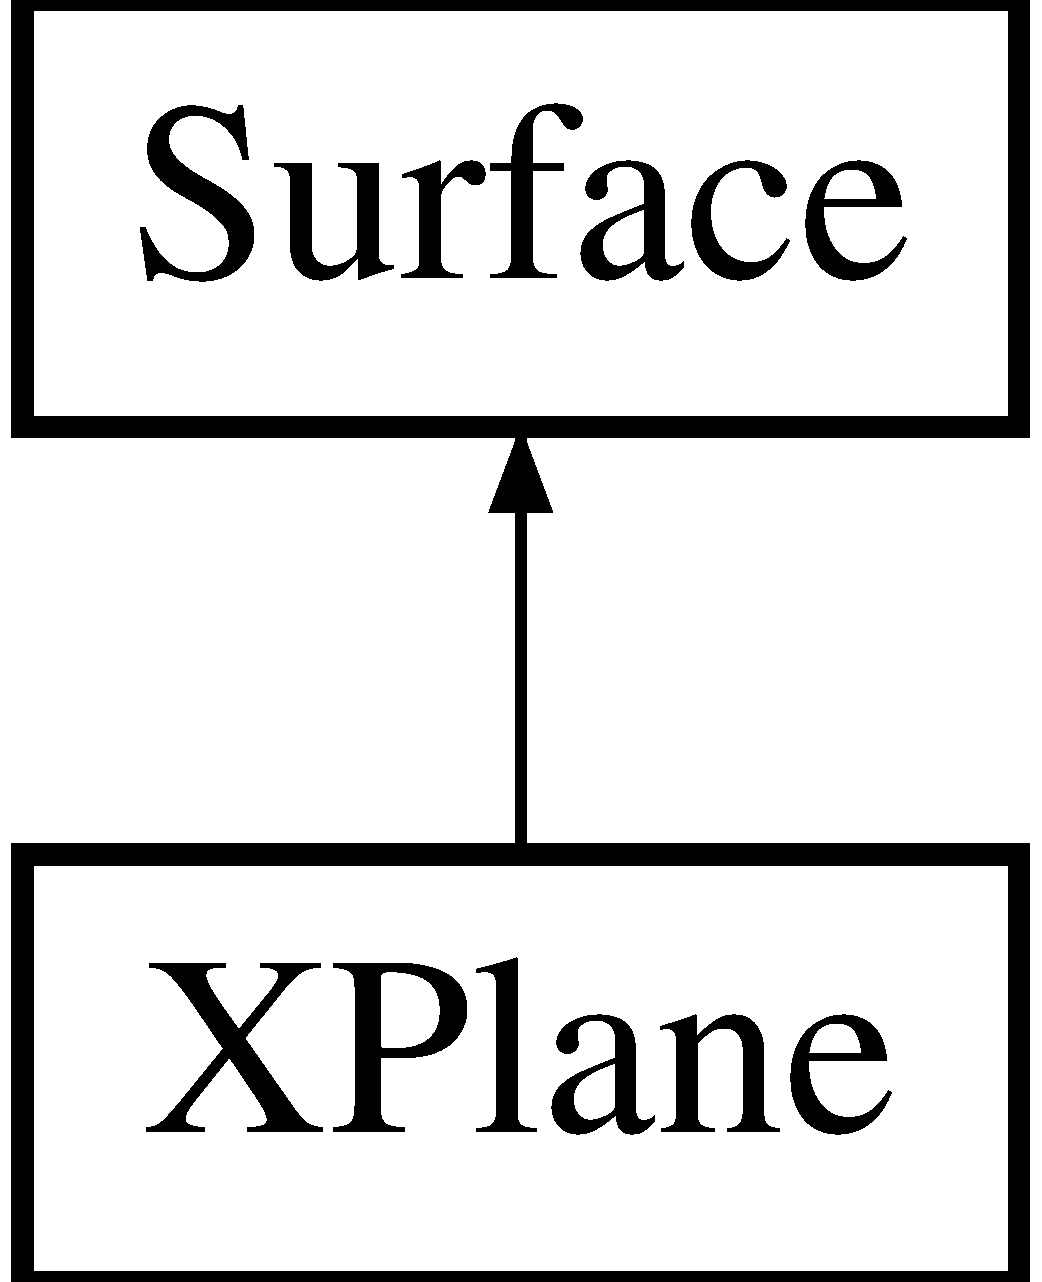
\includegraphics[height=2.000000cm]{classXPlane}
\end{center}
\end{figure}
\subsection*{Public Member Functions}
\begin{DoxyCompactItemize}
\item 
\hyperlink{classXPlane_a0bfa015e8f955be0eef4cfd00f9d81f5}{X\-Plane} ()
\begin{DoxyCompactList}\small\item\em The \hyperlink{classXPlane}{X\-Plane} constructor. \end{DoxyCompactList}\item 
\hypertarget{classXPlane_ada639dc05191d98fc5010a92f47dd105}{virtual \hyperlink{classXPlane_ada639dc05191d98fc5010a92f47dd105}{$\sim$\-X\-Plane} ()}\label{classXPlane_ada639dc05191d98fc5010a92f47dd105}

\begin{DoxyCompactList}\small\item\em \hyperlink{classXPlane}{X\-Plane} destructor. \end{DoxyCompactList}\item 
float \hyperlink{classXPlane_a7dc0803dc4f83aab3de306f4b70a097c}{get\-X} ()
\begin{DoxyCompactList}\small\item\em Returns the x-\/coordinate of the plane's intersection point with the x-\/axis. \end{DoxyCompactList}\item 
void \hyperlink{classXPlane_aad3f4f68ce1cac31589ee00244e30f64}{set\-X} (float x)
\begin{DoxyCompactList}\small\item\em Sets the x-\/coordinate of the plane's intersection point with the x-\/axis. \end{DoxyCompactList}\item 
float \hyperlink{classXPlane_a4370395de84303e337c12457b862753a}{compute\-Nearest\-Distance} (\hyperlink{structneutron}{neutron} $\ast$\hyperlink{structneutron}{neutron})
\begin{DoxyCompactList}\small\item\em Computes the nearest distance to the \hyperlink{classXPlane}{X\-Plane} along a neutron's trajectory. \end{DoxyCompactList}\item 
bool \hyperlink{classXPlane_aba1824906b2f6ed732646385cb3cb98c}{on\-Surface} (\hyperlink{structneutron}{neutron} $\ast$\hyperlink{structneutron}{neutron})
\begin{DoxyCompactList}\small\item\em Checks whether a neutron is on the \hyperlink{classXPlane}{X\-Plane}. \end{DoxyCompactList}\end{DoxyCompactItemize}
\subsection*{Private Attributes}
\begin{DoxyCompactItemize}
\item 
float \hyperlink{classXPlane_a697098fb72495ec39e947938c71db40c}{\-\_\-x}
\end{DoxyCompactItemize}
\subsection*{Additional Inherited Members}


\subsection{Detailed Description}
The \hyperlink{classXPlane}{X\-Plane} is a plane perpendicular to the y-\/axis. 

The \hyperlink{classXPlane}{X\-Plane} represents planes perpendicular to the x-\/axis using the quadratic surface formulation. The \hyperlink{classXPlane}{X\-Plane} is a \hyperlink{classSurface}{Surface} subclass. 

\subsection{Constructor \& Destructor Documentation}
\hypertarget{classXPlane_a0bfa015e8f955be0eef4cfd00f9d81f5}{\index{X\-Plane@{X\-Plane}!X\-Plane@{X\-Plane}}
\index{X\-Plane@{X\-Plane}!XPlane@{X\-Plane}}
\subsubsection[{X\-Plane}]{\setlength{\rightskip}{0pt plus 5cm}X\-Plane\-::\-X\-Plane (
\begin{DoxyParamCaption}
{}
\end{DoxyParamCaption}
)}}\label{classXPlane_a0bfa015e8f955be0eef4cfd00f9d81f5}


The \hyperlink{classXPlane}{X\-Plane} constructor. 

Assigns a default value of x=0 for the x-\/axis intersection point. 

\subsection{Member Function Documentation}
\hypertarget{classXPlane_a4370395de84303e337c12457b862753a}{\index{X\-Plane@{X\-Plane}!compute\-Nearest\-Distance@{compute\-Nearest\-Distance}}
\index{compute\-Nearest\-Distance@{compute\-Nearest\-Distance}!XPlane@{X\-Plane}}
\subsubsection[{compute\-Nearest\-Distance}]{\setlength{\rightskip}{0pt plus 5cm}float X\-Plane\-::compute\-Nearest\-Distance (
\begin{DoxyParamCaption}
\item[{{\bf neutron} $\ast$}]{neutron}
\end{DoxyParamCaption}
)\hspace{0.3cm}{\ttfamily [virtual]}}}\label{classXPlane_a4370395de84303e337c12457b862753a}


Computes the nearest distance to the \hyperlink{classXPlane}{X\-Plane} along a neutron's trajectory. 


\begin{DoxyParams}{Parameters}
{\em neutron} & a pointer to a Neutron struct \\
\hline
\end{DoxyParams}


Implements \hyperlink{classSurface_a3d33dd138200489112a2369eab0b2083}{Surface}.

\hypertarget{classXPlane_a7dc0803dc4f83aab3de306f4b70a097c}{\index{X\-Plane@{X\-Plane}!get\-X@{get\-X}}
\index{get\-X@{get\-X}!XPlane@{X\-Plane}}
\subsubsection[{get\-X}]{\setlength{\rightskip}{0pt plus 5cm}float X\-Plane\-::get\-X (
\begin{DoxyParamCaption}
{}
\end{DoxyParamCaption}
)}}\label{classXPlane_a7dc0803dc4f83aab3de306f4b70a097c}


Returns the x-\/coordinate of the plane's intersection point with the x-\/axis. 

\begin{DoxyReturn}{Returns}
the x-\/coordinate of the intersection point 
\end{DoxyReturn}
\hypertarget{classXPlane_aba1824906b2f6ed732646385cb3cb98c}{\index{X\-Plane@{X\-Plane}!on\-Surface@{on\-Surface}}
\index{on\-Surface@{on\-Surface}!XPlane@{X\-Plane}}
\subsubsection[{on\-Surface}]{\setlength{\rightskip}{0pt plus 5cm}bool X\-Plane\-::on\-Surface (
\begin{DoxyParamCaption}
\item[{{\bf neutron} $\ast$}]{neutron}
\end{DoxyParamCaption}
)\hspace{0.3cm}{\ttfamily [virtual]}}}\label{classXPlane_aba1824906b2f6ed732646385cb3cb98c}


Checks whether a neutron is on the \hyperlink{classXPlane}{X\-Plane}. 

The threshold used to compute whether or not a neutron is on the on the \hyperlink{classXPlane}{X\-Plane} is 1\-E-\/6 for the difference between the x-\/coordinate of the neutron's position and the location of the \hyperlink{classXPlane}{X\-Plane}. 
\begin{DoxyParams}{Parameters}
{\em neutron} & the neutron of interest \\
\hline
\end{DoxyParams}
\begin{DoxyReturn}{Returns}
true if on the \hyperlink{classXPlane}{X\-Plane}, otherwise false 
\end{DoxyReturn}


Implements \hyperlink{classSurface_acdf69fa01f522393ab504b331d88821a}{Surface}.

\hypertarget{classXPlane_aad3f4f68ce1cac31589ee00244e30f64}{\index{X\-Plane@{X\-Plane}!set\-X@{set\-X}}
\index{set\-X@{set\-X}!XPlane@{X\-Plane}}
\subsubsection[{set\-X}]{\setlength{\rightskip}{0pt plus 5cm}void X\-Plane\-::set\-X (
\begin{DoxyParamCaption}
\item[{float}]{x}
\end{DoxyParamCaption}
)}}\label{classXPlane_aad3f4f68ce1cac31589ee00244e30f64}


Sets the x-\/coordinate of the plane's intersection point with the x-\/axis. 


\begin{DoxyParams}{Parameters}
{\em x} & the x-\/coordinate of the intersectiont point \\
\hline
\end{DoxyParams}


\subsection{Member Data Documentation}
\hypertarget{classXPlane_a697098fb72495ec39e947938c71db40c}{\index{X\-Plane@{X\-Plane}!\-\_\-x@{\-\_\-x}}
\index{\-\_\-x@{\-\_\-x}!XPlane@{X\-Plane}}
\subsubsection[{\-\_\-x}]{\setlength{\rightskip}{0pt plus 5cm}float X\-Plane\-::\-\_\-x\hspace{0.3cm}{\ttfamily [private]}}}\label{classXPlane_a697098fb72495ec39e947938c71db40c}
The location of the plane's intersection with the x-\/axis 

The documentation for this class was generated from the following files\-:\begin{DoxyCompactItemize}
\item 
pinspec/src/\hyperlink{Surface_8h}{Surface.\-h}\item 
pinspec/src/Surface.\-cpp\end{DoxyCompactItemize}

\hypertarget{classYPlane}{\section{Y\-Plane Class Reference}
\label{classYPlane}\index{Y\-Plane@{Y\-Plane}}
}


The \hyperlink{classYPlane}{Y\-Plane} is a a plane perpendicular to the y-\/axis.  




{\ttfamily \#include \char`\"{}pinspec/src/\-Surface.\-h\char`\"{}}

Inheritance diagram for Y\-Plane\-:\begin{figure}[H]
\begin{center}
\leavevmode
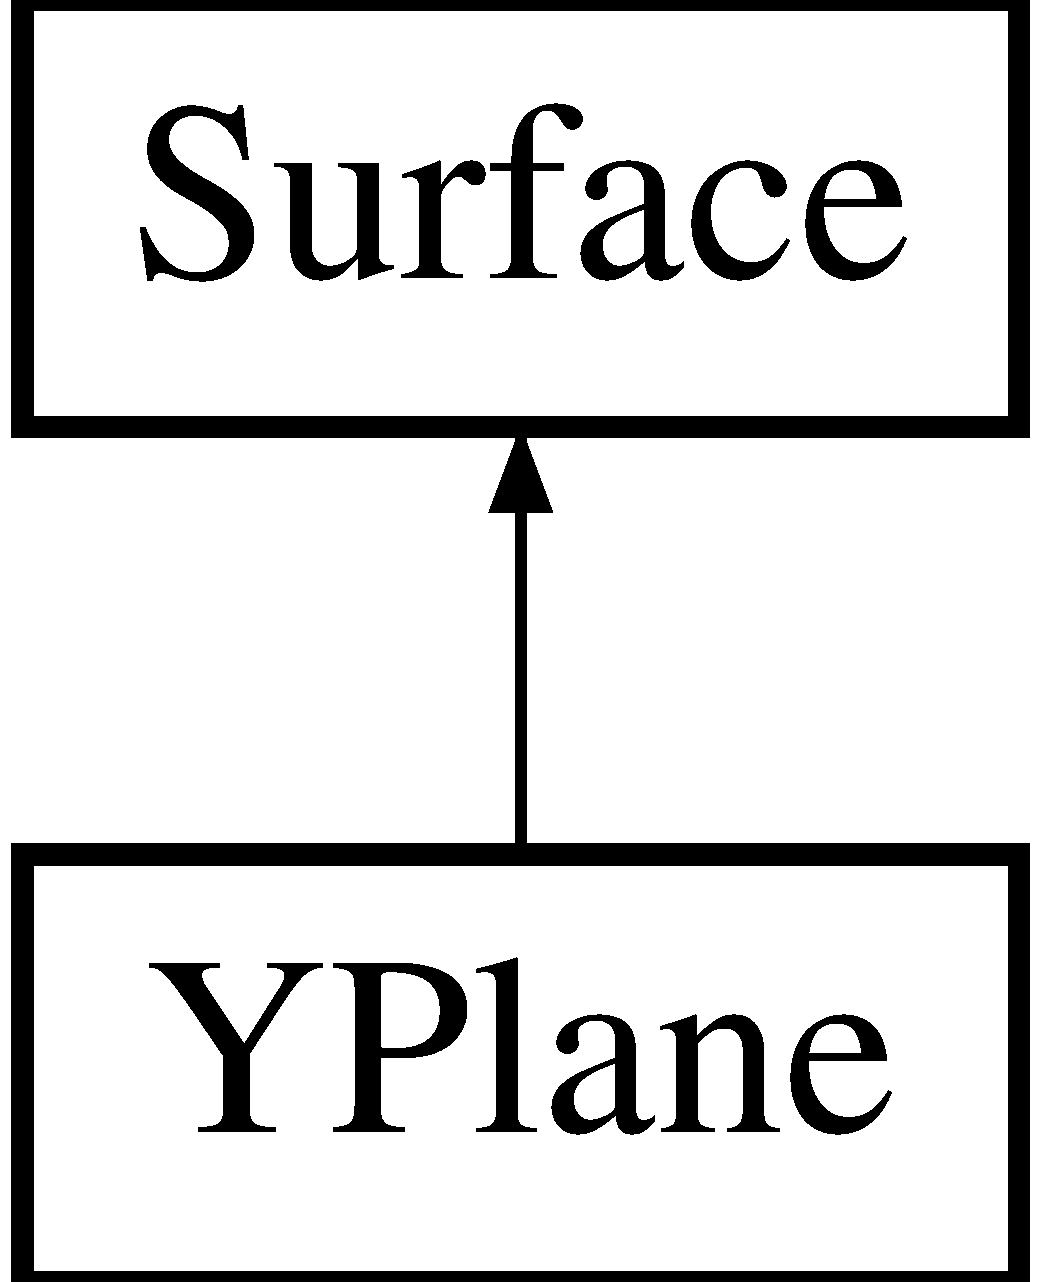
\includegraphics[height=2.000000cm]{classYPlane}
\end{center}
\end{figure}
\subsection*{Public Member Functions}
\begin{DoxyCompactItemize}
\item 
\hyperlink{classYPlane_a3d34dc597f130082af67566a00422f17}{Y\-Plane} ()
\begin{DoxyCompactList}\small\item\em The \hyperlink{classYPlane}{Y\-Plane} constructor. \end{DoxyCompactList}\item 
\hypertarget{classYPlane_a5b76c095cf26194044254f719e92236f}{virtual \hyperlink{classYPlane_a5b76c095cf26194044254f719e92236f}{$\sim$\-Y\-Plane} ()}\label{classYPlane_a5b76c095cf26194044254f719e92236f}

\begin{DoxyCompactList}\small\item\em \hyperlink{classYPlane}{Y\-Plane} destructor. \end{DoxyCompactList}\item 
float \hyperlink{classYPlane_aaba79f83163cc562a3f5e80a3942bc23}{get\-Y} ()
\begin{DoxyCompactList}\small\item\em Returns the y-\/coordinate of the plane's intersection point with the y-\/axis. \end{DoxyCompactList}\item 
void \hyperlink{classYPlane_a3acd886aef57f239f49abdf5004c0df0}{set\-Y} (float y)
\begin{DoxyCompactList}\small\item\em Sets the x-\/coordinate of the plane's intersection point with the y-\/axis. \end{DoxyCompactList}\item 
float \hyperlink{classYPlane_a7f474b38634753235438ca5eff23c2d5}{compute\-Nearest\-Distance} (\hyperlink{structneutron}{neutron} $\ast$\hyperlink{structneutron}{neutron})
\begin{DoxyCompactList}\small\item\em Computes the nearest distance to the \hyperlink{classYPlane}{Y\-Plane} along a neutron's trajectory. \end{DoxyCompactList}\item 
bool \hyperlink{classYPlane_aa8899ff929b56f242316ca684f671772}{on\-Surface} (\hyperlink{structneutron}{neutron} $\ast$\hyperlink{structneutron}{neutron})
\begin{DoxyCompactList}\small\item\em Checks whether a neutron is on the \hyperlink{classYPlane}{Y\-Plane}. \end{DoxyCompactList}\end{DoxyCompactItemize}
\subsection*{Private Attributes}
\begin{DoxyCompactItemize}
\item 
float \hyperlink{classYPlane_a83201c3008efd840a147a136828e6a28}{\-\_\-y}
\end{DoxyCompactItemize}
\subsection*{Additional Inherited Members}


\subsection{Detailed Description}
The \hyperlink{classYPlane}{Y\-Plane} is a a plane perpendicular to the y-\/axis. 

The \hyperlink{classYPlane}{Y\-Plane} represents planes perpendicular to the y-\/axis using the quadratic surface formulation. The \hyperlink{classYPlane}{Y\-Plane} is a \hyperlink{classSurface}{Surface} subclass. 

\subsection{Constructor \& Destructor Documentation}
\hypertarget{classYPlane_a3d34dc597f130082af67566a00422f17}{\index{Y\-Plane@{Y\-Plane}!Y\-Plane@{Y\-Plane}}
\index{Y\-Plane@{Y\-Plane}!YPlane@{Y\-Plane}}
\subsubsection[{Y\-Plane}]{\setlength{\rightskip}{0pt plus 5cm}Y\-Plane\-::\-Y\-Plane (
\begin{DoxyParamCaption}
{}
\end{DoxyParamCaption}
)}}\label{classYPlane_a3d34dc597f130082af67566a00422f17}


The \hyperlink{classYPlane}{Y\-Plane} constructor. 

Assigns a default value of y=0 for the y-\/axis intersection point. 

\subsection{Member Function Documentation}
\hypertarget{classYPlane_a7f474b38634753235438ca5eff23c2d5}{\index{Y\-Plane@{Y\-Plane}!compute\-Nearest\-Distance@{compute\-Nearest\-Distance}}
\index{compute\-Nearest\-Distance@{compute\-Nearest\-Distance}!YPlane@{Y\-Plane}}
\subsubsection[{compute\-Nearest\-Distance}]{\setlength{\rightskip}{0pt plus 5cm}float Y\-Plane\-::compute\-Nearest\-Distance (
\begin{DoxyParamCaption}
\item[{{\bf neutron} $\ast$}]{neutron}
\end{DoxyParamCaption}
)\hspace{0.3cm}{\ttfamily [virtual]}}}\label{classYPlane_a7f474b38634753235438ca5eff23c2d5}


Computes the nearest distance to the \hyperlink{classYPlane}{Y\-Plane} along a neutron's trajectory. 


\begin{DoxyParams}{Parameters}
{\em neutron} & a pointer to a Neutron struct \\
\hline
\end{DoxyParams}


Implements \hyperlink{classSurface_a3d33dd138200489112a2369eab0b2083}{Surface}.

\hypertarget{classYPlane_aaba79f83163cc562a3f5e80a3942bc23}{\index{Y\-Plane@{Y\-Plane}!get\-Y@{get\-Y}}
\index{get\-Y@{get\-Y}!YPlane@{Y\-Plane}}
\subsubsection[{get\-Y}]{\setlength{\rightskip}{0pt plus 5cm}float Y\-Plane\-::get\-Y (
\begin{DoxyParamCaption}
{}
\end{DoxyParamCaption}
)}}\label{classYPlane_aaba79f83163cc562a3f5e80a3942bc23}


Returns the y-\/coordinate of the plane's intersection point with the y-\/axis. 

\begin{DoxyReturn}{Returns}
the y-\/coordinate of the intersection point 
\end{DoxyReturn}
\hypertarget{classYPlane_aa8899ff929b56f242316ca684f671772}{\index{Y\-Plane@{Y\-Plane}!on\-Surface@{on\-Surface}}
\index{on\-Surface@{on\-Surface}!YPlane@{Y\-Plane}}
\subsubsection[{on\-Surface}]{\setlength{\rightskip}{0pt plus 5cm}bool Y\-Plane\-::on\-Surface (
\begin{DoxyParamCaption}
\item[{{\bf neutron} $\ast$}]{neutron}
\end{DoxyParamCaption}
)\hspace{0.3cm}{\ttfamily [virtual]}}}\label{classYPlane_aa8899ff929b56f242316ca684f671772}


Checks whether a neutron is on the \hyperlink{classYPlane}{Y\-Plane}. 

The threshold used to compute whether or not a neutron is on the on the \hyperlink{classYPlane}{Y\-Plane} is 1\-E-\/6 for the difference between the y-\/coordinate of the neutron's position and the location of the \hyperlink{classYPlane}{Y\-Plane} 
\begin{DoxyParams}{Parameters}
{\em neutron} & the neutron of interest to check \\
\hline
\end{DoxyParams}
\begin{DoxyReturn}{Returns}
true if on the \hyperlink{classYPlane}{Y\-Plane}, otherwise false 
\end{DoxyReturn}


Implements \hyperlink{classSurface_acdf69fa01f522393ab504b331d88821a}{Surface}.

\hypertarget{classYPlane_a3acd886aef57f239f49abdf5004c0df0}{\index{Y\-Plane@{Y\-Plane}!set\-Y@{set\-Y}}
\index{set\-Y@{set\-Y}!YPlane@{Y\-Plane}}
\subsubsection[{set\-Y}]{\setlength{\rightskip}{0pt plus 5cm}void Y\-Plane\-::set\-Y (
\begin{DoxyParamCaption}
\item[{float}]{y}
\end{DoxyParamCaption}
)}}\label{classYPlane_a3acd886aef57f239f49abdf5004c0df0}


Sets the x-\/coordinate of the plane's intersection point with the y-\/axis. 


\begin{DoxyParams}{Parameters}
{\em y} & the y-\/coordinate of the intersectiont point \\
\hline
\end{DoxyParams}


\subsection{Member Data Documentation}
\hypertarget{classYPlane_a83201c3008efd840a147a136828e6a28}{\index{Y\-Plane@{Y\-Plane}!\-\_\-y@{\-\_\-y}}
\index{\-\_\-y@{\-\_\-y}!YPlane@{Y\-Plane}}
\subsubsection[{\-\_\-y}]{\setlength{\rightskip}{0pt plus 5cm}float Y\-Plane\-::\-\_\-y\hspace{0.3cm}{\ttfamily [private]}}}\label{classYPlane_a83201c3008efd840a147a136828e6a28}
The location of the plane's intersection with the y-\/axis 

The documentation for this class was generated from the following files\-:\begin{DoxyCompactItemize}
\item 
pinspec/src/\hyperlink{Surface_8h}{Surface.\-h}\item 
pinspec/src/Surface.\-cpp\end{DoxyCompactItemize}

\chapter{File Documentation}
\hypertarget{log_8py}{\section{pinspec/log.py File Reference}
\label{log_8py}\index{pinspec/log.\-py@{pinspec/log.\-py}}
}
\subsection*{Namespaces}
\begin{DoxyCompactItemize}
\item 
namespace \hyperlink{namespacepinspec_1_1log}{pinspec.\-log}
\begin{DoxyCompactList}\small\item\em Utility functions for writing log messages to the screen. \end{DoxyCompactList}\end{DoxyCompactItemize}
\subsection*{Functions}
\begin{DoxyCompactItemize}
\item 
def \hyperlink{namespacepinspec_1_1log_a541e006b2440f460574f9f3017279a1d}{pinspec.\-log.\-py\-\_\-printf}
\begin{DoxyCompactList}\small\item\em Function to print a log message to the screen. \end{DoxyCompactList}\item 
def \hyperlink{namespacepinspec_1_1log_aa886f707adb88128a27972d949cb526f}{pinspec.\-log.\-setlevel}
\begin{DoxyCompactList}\small\item\em Assigns the lowest level logging message. \end{DoxyCompactList}\end{DoxyCompactItemize}


\subsection{Detailed Description}

\hypertarget{plotter_8py}{\section{pinspec/plotter.py File Reference}
\label{plotter_8py}\index{pinspec/plotter.\-py@{pinspec/plotter.\-py}}
}
\subsection*{Namespaces}
\begin{DoxyCompactItemize}
\item 
namespace \hyperlink{namespacepinspec_1_1plotter}{pinspec.\-plotter}
\begin{DoxyCompactList}\small\item\em The plotter module provides utility functions to plot data from P\-I\-N\-S\-P\-E\-C's C++ classes, in particular, tally data and cross-\/sections, thermal scattering P\-D\-Fs/\-C\-D\-Fs, etc. \end{DoxyCompactList}\end{DoxyCompactItemize}
\subsection*{Functions}
\begin{DoxyCompactItemize}
\item 
def \hyperlink{namespacepinspec_1_1plotter_a9310520b2e86be0e353ca47aed9daab1}{pinspec.\-plotter.\-plot\-Micro\-X\-S}
\begin{DoxyCompactList}\small\item\em Plots the microscopoic cross-\/section(s) for one or more reaction rates for an isotope. \end{DoxyCompactList}\item 
def \hyperlink{namespacepinspec_1_1plotter_a43bdaa25a0a79c03b4082523d529f1ef}{pinspec.\-plotter.\-plot\-Macro\-X\-S}
\begin{DoxyCompactList}\small\item\em Plots the macroscopic cross-\/section(s) for one or more reaction rates for a material. \end{DoxyCompactList}\item 
def \hyperlink{namespacepinspec_1_1plotter_a28bc000c574cd5986a481dc2870d7b09}{pinspec.\-plotter.\-plot\-Flux}
\begin{DoxyCompactList}\small\item\em Plots one or more flux tallies by energy. \end{DoxyCompactList}\item 
def \hyperlink{namespacepinspec_1_1plotter_a4ba46d55fc5d6e970c4f4bceefbd1990}{pinspec.\-plotter.\-plot\-Thermal\-Scattering}
\begin{DoxyCompactList}\small\item\em Plots the thermal scattering P\-D\-Fs and C\-D\-Fs for an isotope. \end{DoxyCompactList}\item 
def \hyperlink{namespacepinspec_1_1plotter_a6711829dda3c540c331ff0dce8eacd85}{pinspec.\-plotter.\-plot\-Fission\-Spectrum}
\begin{DoxyCompactList}\small\item\em Plots the fission spectrum P\-D\-F and C\-D\-F. \end{DoxyCompactList}\item 
def \hyperlink{namespacepinspec_1_1plotter_a00729d4934ced6d02844b7f0355b77f4}{pinspec.\-plotter.\-plot\-R\-I}
\begin{DoxyCompactList}\small\item\em Plots a resonance integral (R\-I\-Eff or R\-I\-True) as a step function. \end{DoxyCompactList}\item 
def \hyperlink{namespacepinspec_1_1plotter_afa68183a802e9f9195f30f4eb8f3ae88}{pinspec.\-plotter.\-plot\-Group\-X\-S}
\begin{DoxyCompactList}\small\item\em Plots a multi-\/group cross-\/section as a step function. \end{DoxyCompactList}\end{DoxyCompactItemize}
\subsection*{Variables}
\begin{DoxyCompactItemize}
\item 
\hypertarget{namespacepinspec_1_1plotter_a696ce32dd92f7b9132675df865c1ab5a}{int \hyperlink{namespacepinspec_1_1plotter_a696ce32dd92f7b9132675df865c1ab5a}{pinspec.\-plotter.\-flux\-\_\-plot\-\_\-num} = 0}\label{namespacepinspec_1_1plotter_a696ce32dd92f7b9132675df865c1ab5a}

\begin{DoxyCompactList}\small\item\em A static variable to auto-\/generate unique filenames for flux plots. \end{DoxyCompactList}\item 
\hypertarget{namespacepinspec_1_1plotter_adce9f69349465ff5331b9909723b929b}{string \hyperlink{namespacepinspec_1_1plotter_adce9f69349465ff5331b9909723b929b}{pinspec.\-plotter.\-subdirectory} = \char`\"{}/plots/\char`\"{}}\label{namespacepinspec_1_1plotter_adce9f69349465ff5331b9909723b929b}

\begin{DoxyCompactList}\small\item\em A static variable for the output directory in which to save plots. \end{DoxyCompactList}\end{DoxyCompactItemize}


\subsection{Detailed Description}

\hypertarget{process_8py}{\section{pinspec/process.py File Reference}
\label{process_8py}\index{pinspec/process.\-py@{pinspec/process.\-py}}
}
\subsection*{Classes}
\begin{DoxyCompactItemize}
\item 
class \hyperlink{classpinspec_1_1process_1_1RIEff}{pinspec.\-process.\-R\-I\-Eff}
\begin{DoxyCompactList}\small\item\em An effective resonance integral. \end{DoxyCompactList}\item 
class \hyperlink{classpinspec_1_1process_1_1RITrue}{pinspec.\-process.\-R\-I\-True}
\begin{DoxyCompactList}\small\item\em A true resonance integral. \end{DoxyCompactList}\item 
class \hyperlink{classpinspec_1_1process_1_1GroupXS}{pinspec.\-process.\-Group\-X\-S}
\begin{DoxyCompactList}\small\item\em A multi-\/group cross-\/section for a certain reaction rate. \end{DoxyCompactList}\end{DoxyCompactItemize}
\subsection*{Namespaces}
\begin{DoxyCompactItemize}
\item 
namespace \hyperlink{namespacepinspec_1_1process}{pinspec.\-process}
\begin{DoxyCompactList}\small\item\em The process module provides utility functions to retrieve data from P\-I\-N\-S\-P\-E\-C's C++ classes, in particular, tally data. \end{DoxyCompactList}\end{DoxyCompactItemize}
\subsection*{Functions}
\begin{DoxyCompactItemize}
\item 
def \hyperlink{namespacepinspec_1_1process_a4a994b613e53287a126b8b5263daa6ff}{pinspec.\-process.\-get\-Tally\-Centers}
\begin{DoxyCompactList}\small\item\em Returns an array of the center values for a tally's bins. \end{DoxyCompactList}\item 
def \hyperlink{namespacepinspec_1_1process_a9fd8e784cab1f1c96bd490b212a971c0}{pinspec.\-process.\-get\-Tally\-Edges}
\begin{DoxyCompactList}\small\item\em Returns an array of the bin edge values for a tally's bins. \end{DoxyCompactList}\item 
def \hyperlink{namespacepinspec_1_1process_a8db40966df01a6f67e9cab3c01690964}{pinspec.\-process.\-get\-Tally\-Batch\-Mu}
\begin{DoxyCompactList}\small\item\em Returns an array of the batch averages for the tally's bins. \end{DoxyCompactList}\item 
def \hyperlink{namespacepinspec_1_1process_a8ff9733e706d305e26797cab749b0eee}{pinspec.\-process.\-get\-Tally\-Batch\-Variances}
\begin{DoxyCompactList}\small\item\em Returns an array of the batch variances for a tally's bins. \end{DoxyCompactList}\item 
def \hyperlink{namespacepinspec_1_1process_a10ce7b5adb22e27bd1309a068a7f71ed}{pinspec.\-process.\-get\-Tally\-Batch\-Std\-Dev}
\begin{DoxyCompactList}\small\item\em Returns an array of the batch standard deviations for a tally's bins. \end{DoxyCompactList}\item 
def \hyperlink{namespacepinspec_1_1process_a76f6c9fd781df929bc86b30afffde0a4}{pinspec.\-process.\-get\-Tally\-Batch\-Rel\-Err}
\begin{DoxyCompactList}\small\item\em Returns an array of the batch relative errors for a tally's bins. \end{DoxyCompactList}\item 
def \hyperlink{namespacepinspec_1_1process_ad8268b637d8441c8f3adf739d2682029}{pinspec.\-process.\-get\-Tally\-Batch\-Statistics}
\begin{DoxyCompactList}\small\item\em Returns a 2\-D array of the tally's batch statistics. \end{DoxyCompactList}\item 
def \hyperlink{namespacepinspec_1_1process_a6cf809df65f0a24714f69a080add30b2}{pinspec.\-process.\-print\-Tallies}
\begin{DoxyCompactList}\small\item\em Prints formatted tally batch-\/averaged data to the screen as a table. \end{DoxyCompactList}\item 
def \hyperlink{namespacepinspec_1_1process_afb8cb723f05702c6ab466ef4ffda7a8e}{pinspec.\-process.\-compute\-Mean\-Num\-Collisions}
\begin{DoxyCompactList}\small\item\em Computes the mean number of collisions for a neutron before absorption. \end{DoxyCompactList}\item 
def \hyperlink{namespacepinspec_1_1process_a5a89290e473b171ac1f535ef361e1e83}{pinspec.\-process.\-compute\-Mean\-Neutron\-Lifetime}
\begin{DoxyCompactList}\small\item\em Computes the mean neutron lifetime (seconds) before absorption. \end{DoxyCompactList}\item 
def \hyperlink{namespacepinspec_1_1process_abca578c733031cbf54954e15df72a385}{pinspec.\-process.\-print\-R\-Is}
\begin{DoxyCompactList}\small\item\em Prints a formatted table for an array of true and/or effectrive resonance integrals to the screen. \end{DoxyCompactList}\end{DoxyCompactItemize}


\subsection{Detailed Description}

\hypertarget{slbw_8py}{\section{pinspec/slbw.py File Reference}
\label{slbw_8py}\index{pinspec/slbw.\-py@{pinspec/slbw.\-py}}
}
\subsection*{Namespaces}
\begin{DoxyCompactItemize}
\item 
namespace \hyperlink{namespacepinspec_1_1slbw}{pinspec.\-slbw}
\begin{DoxyCompactList}\small\item\em The slbw module provides utility functions to generate resonant cross-\/sections using the Single-\/\-Level Breit-\/\-Wigner formalism. \end{DoxyCompactList}\end{DoxyCompactItemize}
\subsection*{Functions}
\begin{DoxyCompactItemize}
\item 
def \hyperlink{namespacepinspec_1_1slbw_a4aafba8dacef99e07de3143d25345244}{pinspec.\-slbw.\-S\-L\-B\-W\-X\-S}
\begin{DoxyCompactList}\small\item\em Function to create resonant capture and scatter cross-\/sections. \end{DoxyCompactList}\item 
def \hyperlink{namespacepinspec_1_1slbw_a026e643a6e213703f2b18533c7149c03}{pinspec.\-slbw.\-convert}
\begin{DoxyCompactList}\small\item\em Function to convert a string into a float. \end{DoxyCompactList}\item 
def \hyperlink{namespacepinspec_1_1slbw_a76171c0756809c031a091b2b5bfda666}{pinspec.\-slbw.\-parse}
\begin{DoxyCompactList}\small\item\em Function to parse a string and convert into resonance parameters. \end{DoxyCompactList}\item 
def \hyperlink{namespacepinspec_1_1slbw_a7ebd0410cdcdcfbdc9bb26d6d456cbdf}{pinspec.\-slbw.\-generate\-Potential\-Scattering}
\begin{DoxyCompactList}\small\item\em Function to generate a potential scattering cross-\/section for an isotope based on data in a resonance parameters file. \end{DoxyCompactList}\item 
def \hyperlink{namespacepinspec_1_1slbw_a48b45b1d229e9afa999d8cb5fc201144}{pinspec.\-slbw.\-compare\-X\-S}
\begin{DoxyCompactList}\small\item\em Function to generate a plot of the S\-L\-B\-W generated cross-\/section along with the E\-N\-D\-F-\/\-V\-I\-I version of the cross-\/section for comparison. \end{DoxyCompactList}\end{DoxyCompactItemize}


\subsection{Detailed Description}

\hypertarget{arraycreator_8h}{\section{pinspec/src/arraycreator.h File Reference}
\label{arraycreator_8h}\index{pinspec/src/arraycreator.\-h@{pinspec/src/arraycreator.\-h}}
}


Functions for creating arrays with similar syntax to M\-A\-T\-L\-A\-B.  


\subsection*{Functions}
\begin{DoxyCompactItemize}
\item 
{\footnotesize template$<$typename T , typename U $>$ }\\U $\ast$ \hyperlink{arraycreator_8h_a903d5591003f40018b94df01cb30a13b}{linspace} (T start, T end, int num\-\_\-values)
\begin{DoxyCompactList}\small\item\em Creates an array of equally spaced values. \end{DoxyCompactList}\item 
{\footnotesize template$<$typename T , typename U $>$ }\\U $\ast$ \hyperlink{arraycreator_8h_a1f3c9394316bb80f901c7b1d57d0270c}{logspace} (T start, T end, int num\-\_\-values)
\begin{DoxyCompactList}\small\item\em Creates an array of equal logarithmically spaced values. \end{DoxyCompactList}\end{DoxyCompactItemize}


\subsection{Detailed Description}
Functions for creating arrays with similar syntax to M\-A\-T\-L\-A\-B. \begin{DoxyAuthor}{Author}
William Boyd (\href{mailto:wboyd@mit.edu}{\tt wboyd@mit.\-edu}) 
\end{DoxyAuthor}
\begin{DoxyDate}{Date}
March 28, 2012 
\end{DoxyDate}


\subsection{Function Documentation}
\hypertarget{arraycreator_8h_a903d5591003f40018b94df01cb30a13b}{\index{arraycreator.\-h@{arraycreator.\-h}!linspace@{linspace}}
\index{linspace@{linspace}!arraycreator.h@{arraycreator.\-h}}
\subsubsection[{linspace}]{\setlength{\rightskip}{0pt plus 5cm}template$<$typename T , typename U $>$ U$\ast$ linspace (
\begin{DoxyParamCaption}
\item[{T}]{start, }
\item[{T}]{end, }
\item[{int}]{num\-\_\-values}
\end{DoxyParamCaption}
)}}\label{arraycreator_8h_a903d5591003f40018b94df01cb30a13b}


Creates an array of equally spaced values. 

Helper function to generate an array of equally spaced values between a specified start and end point. Modeled after M\-A\-T\-L\-A\-B's linspace function. 
\begin{DoxyParams}{Parameters}
{\em start} & the starting point \\
\hline
{\em end} & the ending point \\
\hline
{\em num\-\_\-values} & the number of values to create \\
\hline
\end{DoxyParams}
\begin{DoxyReturn}{Returns}
a pointer to the array of points 
\end{DoxyReturn}
\hypertarget{arraycreator_8h_a1f3c9394316bb80f901c7b1d57d0270c}{\index{arraycreator.\-h@{arraycreator.\-h}!logspace@{logspace}}
\index{logspace@{logspace}!arraycreator.h@{arraycreator.\-h}}
\subsubsection[{logspace}]{\setlength{\rightskip}{0pt plus 5cm}template$<$typename T , typename U $>$ U$\ast$ logspace (
\begin{DoxyParamCaption}
\item[{T}]{start, }
\item[{T}]{end, }
\item[{int}]{num\-\_\-values}
\end{DoxyParamCaption}
)}}\label{arraycreator_8h_a1f3c9394316bb80f901c7b1d57d0270c}


Creates an array of equal logarithmically spaced values. 

Helper function to generate an array of equal logarithmically spaced values between a specified start and end point. Modeled after M\-A\-T\-L\-A\-B's logspace function. 
\begin{DoxyParams}{Parameters}
{\em start} & the starting point \\
\hline
{\em end} & the ending point \\
\hline
{\em num\-\_\-values} & the number of values to create \\
\hline
\end{DoxyParams}
\begin{DoxyReturn}{Returns}
a pointer to the array of points 
\end{DoxyReturn}

\hypertarget{Fissioner_8h}{\section{pinspec/src/\-Fissioner.h File Reference}
\label{Fissioner_8h}\index{pinspec/src/\-Fissioner.\-h@{pinspec/src/\-Fissioner.\-h}}
}


The \hyperlink{classFissioner}{Fissioner} class for fission neutron emission.  


\subsection*{Classes}
\begin{DoxyCompactItemize}
\item 
class \hyperlink{classFissioner}{Fissioner}
\begin{DoxyCompactList}\small\item\em The \hyperlink{classFissioner}{Fissioner} represents the physics of fission neutron emission. \end{DoxyCompactList}\end{DoxyCompactItemize}


\subsection{Detailed Description}
The \hyperlink{classFissioner}{Fissioner} class for fission neutron emission. \begin{DoxyAuthor}{Author}
William Boyd (\href{mailto:wboyd@mit.edu}{\tt wboyd@mit.\-edu}) 
\end{DoxyAuthor}
\begin{DoxyDate}{Date}
March 15, 2012 
\end{DoxyDate}

\hypertarget{Geometry_8h}{\section{Geometry.\-h File Reference}
\label{Geometry_8h}\index{Geometry.\-h@{Geometry.\-h}}
}


The \hyperlink{classGeometry}{Geometry} class.  


\subsection*{Classes}
\begin{DoxyCompactItemize}
\item 
class \hyperlink{classGeometry}{Geometry}
\begin{DoxyCompactList}\small\item\em The \hyperlink{classGeometry}{Geometry} represents the highest level entity in which a neutron may reside during a P\-I\-N\-S\-P\-E\-C simulaiton. The geometry consists of one or more regions and controls the highest level Monte Carlo kernel. \end{DoxyCompactList}\end{DoxyCompactItemize}
\subsection*{Typedefs}
\begin{DoxyCompactItemize}
\item 
\hypertarget{Geometry_8h_af321382c4a8d9fdb71c83382f82fac00}{typedef enum \hyperlink{Geometry_8h_ab8a71cfbb692cd5df3176bc4888e6b62}{spatial\-Types} \hyperlink{Geometry_8h_af321382c4a8d9fdb71c83382f82fac00}{spatial\-Type}}\label{Geometry_8h_af321382c4a8d9fdb71c83382f82fac00}

\begin{DoxyCompactList}\small\item\em A spatial type for the geometry. \end{DoxyCompactList}\end{DoxyCompactItemize}
\subsection*{Enumerations}
\begin{DoxyCompactItemize}
\item 
enum \hyperlink{Geometry_8h_ab8a71cfbb692cd5df3176bc4888e6b62}{spatial\-Types} \{ \hyperlink{Geometry_8h_ab8a71cfbb692cd5df3176bc4888e6b62a5e81317429db7020ae01f253012683a8}{I\-N\-F\-I\-N\-I\-T\-E\-\_\-\-H\-O\-M\-O\-G\-E\-N\-E\-O\-U\-S}, 
\hyperlink{Geometry_8h_ab8a71cfbb692cd5df3176bc4888e6b62a936d77141db108a17400f383c47f7532}{H\-O\-M\-O\-G\-E\-N\-E\-O\-U\-S\-\_\-\-E\-Q\-U\-I\-V\-A\-L\-E\-N\-C\-E}, 
\hyperlink{Geometry_8h_ab8a71cfbb692cd5df3176bc4888e6b62ab01ed1e719765219766569c22e20d3f0}{H\-E\-T\-E\-R\-O\-G\-E\-N\-E\-O\-U\-S}
 \}
\begin{DoxyCompactList}\small\item\em The spatial types for the geometry. \end{DoxyCompactList}\end{DoxyCompactItemize}


\subsection{Detailed Description}
The \hyperlink{classGeometry}{Geometry} class. \begin{DoxyAuthor}{Author}
William Boyd (\href{mailto:wboyd@mit.edu}{\tt wboyd@mit.\-edu}) 
\end{DoxyAuthor}
\begin{DoxyDate}{Date}
March 6, 2013. 
\end{DoxyDate}


\subsection{Enumeration Type Documentation}
\hypertarget{Geometry_8h_ab8a71cfbb692cd5df3176bc4888e6b62}{\index{Geometry.\-h@{Geometry.\-h}!spatial\-Types@{spatial\-Types}}
\index{spatial\-Types@{spatial\-Types}!Geometry.h@{Geometry.\-h}}
\subsubsection[{spatial\-Types}]{\setlength{\rightskip}{0pt plus 5cm}enum {\bf spatial\-Types}}}\label{Geometry_8h_ab8a71cfbb692cd5df3176bc4888e6b62}


The spatial types for the geometry. 

\begin{Desc}
\item[Enumerator\-: ]\par
\begin{description}
\index{I\-N\-F\-I\-N\-I\-T\-E\-\_\-\-H\-O\-M\-O\-G\-E\-N\-E\-O\-U\-S@{I\-N\-F\-I\-N\-I\-T\-E\-\_\-\-H\-O\-M\-O\-G\-E\-N\-E\-O\-U\-S}!Geometry.\-h@{Geometry.\-h}}\index{Geometry.\-h@{Geometry.\-h}!I\-N\-F\-I\-N\-I\-T\-E\-\_\-\-H\-O\-M\-O\-G\-E\-N\-E\-O\-U\-S@{I\-N\-F\-I\-N\-I\-T\-E\-\_\-\-H\-O\-M\-O\-G\-E\-N\-E\-O\-U\-S}}\item[{\em 
\hypertarget{Geometry_8h_ab8a71cfbb692cd5df3176bc4888e6b62a5e81317429db7020ae01f253012683a8}{I\-N\-F\-I\-N\-I\-T\-E\-\_\-\-H\-O\-M\-O\-G\-E\-N\-E\-O\-U\-S}\label{Geometry_8h_ab8a71cfbb692cd5df3176bc4888e6b62a5e81317429db7020ae01f253012683a8}
}]An infinite homogeneous medium \index{H\-O\-M\-O\-G\-E\-N\-E\-O\-U\-S\-\_\-\-E\-Q\-U\-I\-V\-A\-L\-E\-N\-C\-E@{H\-O\-M\-O\-G\-E\-N\-E\-O\-U\-S\-\_\-\-E\-Q\-U\-I\-V\-A\-L\-E\-N\-C\-E}!Geometry.\-h@{Geometry.\-h}}\index{Geometry.\-h@{Geometry.\-h}!H\-O\-M\-O\-G\-E\-N\-E\-O\-U\-S\-\_\-\-E\-Q\-U\-I\-V\-A\-L\-E\-N\-C\-E@{H\-O\-M\-O\-G\-E\-N\-E\-O\-U\-S\-\_\-\-E\-Q\-U\-I\-V\-A\-L\-E\-N\-C\-E}}\item[{\em 
\hypertarget{Geometry_8h_ab8a71cfbb692cd5df3176bc4888e6b62a936d77141db108a17400f383c47f7532}{H\-O\-M\-O\-G\-E\-N\-E\-O\-U\-S\-\_\-\-E\-Q\-U\-I\-V\-A\-L\-E\-N\-C\-E}\label{Geometry_8h_ab8a71cfbb692cd5df3176bc4888e6b62a936d77141db108a17400f383c47f7532}
}]A heterogeneous-\/homogeneous equivalent geometry \index{H\-E\-T\-E\-R\-O\-G\-E\-N\-E\-O\-U\-S@{H\-E\-T\-E\-R\-O\-G\-E\-N\-E\-O\-U\-S}!Geometry.\-h@{Geometry.\-h}}\index{Geometry.\-h@{Geometry.\-h}!H\-E\-T\-E\-R\-O\-G\-E\-N\-E\-O\-U\-S@{H\-E\-T\-E\-R\-O\-G\-E\-N\-E\-O\-U\-S}}\item[{\em 
\hypertarget{Geometry_8h_ab8a71cfbb692cd5df3176bc4888e6b62ab01ed1e719765219766569c22e20d3f0}{H\-E\-T\-E\-R\-O\-G\-E\-N\-E\-O\-U\-S}\label{Geometry_8h_ab8a71cfbb692cd5df3176bc4888e6b62ab01ed1e719765219766569c22e20d3f0}
}]A heterogenous geometry built of regions and surfaces \end{description}
\end{Desc}


\hypertarget{integrate_8h}{\section{integrate.\-h File Reference}
\label{integrate_8h}\index{integrate.\-h@{integrate.\-h}}
}


Utility functions for numerical integration of 1\-D functions.  


\subsection*{Typedefs}
\begin{DoxyCompactItemize}
\item 
\hypertarget{integrate_8h_aa160402da29525855473b83b57814f1b}{typedef enum \hyperlink{integrate_8h_a4bd85a3f1a50940978504c3e4e43b04d}{integration\-Schemes} \hyperlink{integrate_8h_aa160402da29525855473b83b57814f1b}{integration\-Scheme}}\label{integrate_8h_aa160402da29525855473b83b57814f1b}

\begin{DoxyCompactList}\small\item\em Numerical integration methods. \end{DoxyCompactList}\end{DoxyCompactItemize}
\subsection*{Enumerations}
\begin{DoxyCompactItemize}
\item 
enum \hyperlink{integrate_8h_a4bd85a3f1a50940978504c3e4e43b04d}{integration\-Schemes} \{ \\*
\hyperlink{integrate_8h_a4bd85a3f1a50940978504c3e4e43b04dafc2a7695ad9bb18a55fb67de858e97f1}{R\-I\-E\-M\-A\-N\-N\-\_\-\-L\-E\-F\-T}, 
\hyperlink{integrate_8h_a4bd85a3f1a50940978504c3e4e43b04da881bbba9969e1dd00c92f0d0531285ab}{R\-I\-E\-M\-A\-N\-N\-\_\-\-R\-I\-G\-H\-T}, 
\hyperlink{integrate_8h_a4bd85a3f1a50940978504c3e4e43b04daceaf3f038b41d438fe877b6a804e1274}{R\-I\-E\-M\-A\-N\-N\-\_\-\-C\-E\-N\-T\-E\-R}, 
\hyperlink{integrate_8h_a4bd85a3f1a50940978504c3e4e43b04da492124afa39e48a6ceb6b989957e8e65}{T\-R\-A\-P\-E\-Z\-O\-I\-D\-A\-L}, 
\\*
\hyperlink{integrate_8h_a4bd85a3f1a50940978504c3e4e43b04daae47caa042f20199c0f74b03c7596b3e}{S\-I\-M\-P\-S\-O\-N\-S}, 
\hyperlink{integrate_8h_a4bd85a3f1a50940978504c3e4e43b04dace15dccf7da34ce361e6aede1c120cbc}{S\-I\-M\-P\-S\-O\-N\-S38}, 
\hyperlink{integrate_8h_a4bd85a3f1a50940978504c3e4e43b04daef4dd4bf91b70773492df324d5769f58}{B\-O\-O\-L\-E\-S}
 \}
\begin{DoxyCompactList}\small\item\em Numerical integration methods. \end{DoxyCompactList}\end{DoxyCompactItemize}
\subsection*{Functions}
\begin{DoxyCompactItemize}
\item 
{\footnotesize template$<$typename T , typename U $>$ }\\void \hyperlink{integrate_8h_a6986dcb4f4d8dce75ba3a907b9da75aa}{cumulative\-Integral} (T $\ast$x, T $\ast$y, U $\ast$cdf, int length, \hyperlink{integrate_8h_aa160402da29525855473b83b57814f1b}{integration\-Scheme} scheme)
\begin{DoxyCompactList}\small\item\em Performs a cumulative numerical integral over arrays of x and y values using the specificed integration method. \end{DoxyCompactList}\item 
{\footnotesize template$<$typename T $>$ }\\double \hyperlink{integrate_8h_a6343365f0d65a315eae7cc641f2732af}{compute\-Riemann\-Left} (T $\ast$x, T $\ast$y, int length)
\begin{DoxyCompactList}\small\item\em Performs a numerical integral using the left-\/centered Riemann numerical integration method. \end{DoxyCompactList}\item 
{\footnotesize template$<$typename T $>$ }\\double \hyperlink{integrate_8h_af71a2826d64f1615a6e7c8e01688b675}{compute\-Riemann\-Right} (T $\ast$x, T $\ast$y, int length)
\begin{DoxyCompactList}\small\item\em Performs a numerical integral using the right-\/centered Riemann numerical integration method. \end{DoxyCompactList}\item 
{\footnotesize template$<$typename T $>$ }\\double \hyperlink{integrate_8h_ad4dfff0713192e61bd14a825ec198af7}{compute\-Riemann\-Center} (T $\ast$x, T $\ast$y, int length)
\begin{DoxyCompactList}\small\item\em Performs a numerical integral using the midpoint-\/centered Riemann numerical integration method. \end{DoxyCompactList}\item 
{\footnotesize template$<$typename T $>$ }\\double \hyperlink{integrate_8h_a7b5a20ca959bc8a9b55c41c5f1dffcca}{compute\-Trapezoidal} (T $\ast$x, T $\ast$y, int length)
\begin{DoxyCompactList}\small\item\em Performs a numerical integral using the trapezoidal numerical integration method. \end{DoxyCompactList}\item 
{\footnotesize template$<$typename T $>$ }\\double \hyperlink{integrate_8h_ac5a99a2d09d82e7c531868271bdb532f}{compute\-Simpsons} (T $\ast$x, T $\ast$y, int length)
\begin{DoxyCompactList}\small\item\em Performs a numerical integral using the Simpson's numerical integration method. \end{DoxyCompactList}\item 
{\footnotesize template$<$typename T $>$ }\\double \hyperlink{integrate_8h_a24c3c46489d761340e9e1685925b110c}{compute\-Simpsons38} (T $\ast$x, T $\ast$y, int length)
\begin{DoxyCompactList}\small\item\em Performs a numerical integral using the Simpson's 3/8ths numerical integration method. \end{DoxyCompactList}\item 
{\footnotesize template$<$typename T $>$ }\\double \hyperlink{integrate_8h_ae98eaa91a738695a69473f278b4e8b14}{compute\-Booles} (T $\ast$x, T $\ast$y, int length)
\begin{DoxyCompactList}\small\item\em Performs a numerical integral using the Boole's numerical integration method. \end{DoxyCompactList}\item 
{\footnotesize template$<$typename T $>$ }\\double \hyperlink{integrate_8h_a4b658e4034d56348ca7dd65aee07d64a}{integrate} (T $\ast$x, T $\ast$y, int length, \hyperlink{integrate_8h_aa160402da29525855473b83b57814f1b}{integration\-Scheme} scheme)
\begin{DoxyCompactList}\small\item\em Performs a 1\-D numerical integral over arrays of x and y values using the specified integration scheme. \end{DoxyCompactList}\end{DoxyCompactItemize}


\subsection{Detailed Description}
Utility functions for numerical integration of 1\-D functions. This module provides a set of templated integration methods for both normal numerical integration and cumulative numerical integration. It implements the Riemann integration method with left-\/aligned, right-\/aligned and midpoint methods, the trapezoidal integration, and higher-\/order Simpsons, Simpson's 3/8ths and Boole's methods. \begin{DoxyAuthor}{Author}
William Boyd (\href{mailto:wboyd@mit.edu}{\tt wboyd@mit.\-edu}) 
\end{DoxyAuthor}
\begin{DoxyDate}{Date}
February 9, 2012 
\end{DoxyDate}


\subsection{Enumeration Type Documentation}
\hypertarget{integrate_8h_a4bd85a3f1a50940978504c3e4e43b04d}{\index{integrate.\-h@{integrate.\-h}!integration\-Schemes@{integration\-Schemes}}
\index{integration\-Schemes@{integration\-Schemes}!integrate.h@{integrate.\-h}}
\subsubsection[{integration\-Schemes}]{\setlength{\rightskip}{0pt plus 5cm}enum {\bf integration\-Schemes}}}\label{integrate_8h_a4bd85a3f1a50940978504c3e4e43b04d}


Numerical integration methods. 

\begin{Desc}
\item[Enumerator\-: ]\par
\begin{description}
\index{R\-I\-E\-M\-A\-N\-N\-\_\-\-L\-E\-F\-T@{R\-I\-E\-M\-A\-N\-N\-\_\-\-L\-E\-F\-T}!integrate.\-h@{integrate.\-h}}\index{integrate.\-h@{integrate.\-h}!R\-I\-E\-M\-A\-N\-N\-\_\-\-L\-E\-F\-T@{R\-I\-E\-M\-A\-N\-N\-\_\-\-L\-E\-F\-T}}\item[{\em 
\hypertarget{integrate_8h_a4bd85a3f1a50940978504c3e4e43b04dafc2a7695ad9bb18a55fb67de858e97f1}{R\-I\-E\-M\-A\-N\-N\-\_\-\-L\-E\-F\-T}\label{integrate_8h_a4bd85a3f1a50940978504c3e4e43b04dafc2a7695ad9bb18a55fb67de858e97f1}
}]Left-\/aligned Riemann integration method \index{R\-I\-E\-M\-A\-N\-N\-\_\-\-R\-I\-G\-H\-T@{R\-I\-E\-M\-A\-N\-N\-\_\-\-R\-I\-G\-H\-T}!integrate.\-h@{integrate.\-h}}\index{integrate.\-h@{integrate.\-h}!R\-I\-E\-M\-A\-N\-N\-\_\-\-R\-I\-G\-H\-T@{R\-I\-E\-M\-A\-N\-N\-\_\-\-R\-I\-G\-H\-T}}\item[{\em 
\hypertarget{integrate_8h_a4bd85a3f1a50940978504c3e4e43b04da881bbba9969e1dd00c92f0d0531285ab}{R\-I\-E\-M\-A\-N\-N\-\_\-\-R\-I\-G\-H\-T}\label{integrate_8h_a4bd85a3f1a50940978504c3e4e43b04da881bbba9969e1dd00c92f0d0531285ab}
}]Right-\/aligned Riemann integration method \index{R\-I\-E\-M\-A\-N\-N\-\_\-\-C\-E\-N\-T\-E\-R@{R\-I\-E\-M\-A\-N\-N\-\_\-\-C\-E\-N\-T\-E\-R}!integrate.\-h@{integrate.\-h}}\index{integrate.\-h@{integrate.\-h}!R\-I\-E\-M\-A\-N\-N\-\_\-\-C\-E\-N\-T\-E\-R@{R\-I\-E\-M\-A\-N\-N\-\_\-\-C\-E\-N\-T\-E\-R}}\item[{\em 
\hypertarget{integrate_8h_a4bd85a3f1a50940978504c3e4e43b04daceaf3f038b41d438fe877b6a804e1274}{R\-I\-E\-M\-A\-N\-N\-\_\-\-C\-E\-N\-T\-E\-R}\label{integrate_8h_a4bd85a3f1a50940978504c3e4e43b04daceaf3f038b41d438fe877b6a804e1274}
}]Midpoint Riemann integration method \index{T\-R\-A\-P\-E\-Z\-O\-I\-D\-A\-L@{T\-R\-A\-P\-E\-Z\-O\-I\-D\-A\-L}!integrate.\-h@{integrate.\-h}}\index{integrate.\-h@{integrate.\-h}!T\-R\-A\-P\-E\-Z\-O\-I\-D\-A\-L@{T\-R\-A\-P\-E\-Z\-O\-I\-D\-A\-L}}\item[{\em 
\hypertarget{integrate_8h_a4bd85a3f1a50940978504c3e4e43b04da492124afa39e48a6ceb6b989957e8e65}{T\-R\-A\-P\-E\-Z\-O\-I\-D\-A\-L}\label{integrate_8h_a4bd85a3f1a50940978504c3e4e43b04da492124afa39e48a6ceb6b989957e8e65}
}]Trapezoidal integration method \index{S\-I\-M\-P\-S\-O\-N\-S@{S\-I\-M\-P\-S\-O\-N\-S}!integrate.\-h@{integrate.\-h}}\index{integrate.\-h@{integrate.\-h}!S\-I\-M\-P\-S\-O\-N\-S@{S\-I\-M\-P\-S\-O\-N\-S}}\item[{\em 
\hypertarget{integrate_8h_a4bd85a3f1a50940978504c3e4e43b04daae47caa042f20199c0f74b03c7596b3e}{S\-I\-M\-P\-S\-O\-N\-S}\label{integrate_8h_a4bd85a3f1a50940978504c3e4e43b04daae47caa042f20199c0f74b03c7596b3e}
}]Simpson's integration method \index{S\-I\-M\-P\-S\-O\-N\-S38@{S\-I\-M\-P\-S\-O\-N\-S38}!integrate.\-h@{integrate.\-h}}\index{integrate.\-h@{integrate.\-h}!S\-I\-M\-P\-S\-O\-N\-S38@{S\-I\-M\-P\-S\-O\-N\-S38}}\item[{\em 
\hypertarget{integrate_8h_a4bd85a3f1a50940978504c3e4e43b04dace15dccf7da34ce361e6aede1c120cbc}{S\-I\-M\-P\-S\-O\-N\-S38}\label{integrate_8h_a4bd85a3f1a50940978504c3e4e43b04dace15dccf7da34ce361e6aede1c120cbc}
}]Simpson's 3/8ths integration method \index{B\-O\-O\-L\-E\-S@{B\-O\-O\-L\-E\-S}!integrate.\-h@{integrate.\-h}}\index{integrate.\-h@{integrate.\-h}!B\-O\-O\-L\-E\-S@{B\-O\-O\-L\-E\-S}}\item[{\em 
\hypertarget{integrate_8h_a4bd85a3f1a50940978504c3e4e43b04daef4dd4bf91b70773492df324d5769f58}{B\-O\-O\-L\-E\-S}\label{integrate_8h_a4bd85a3f1a50940978504c3e4e43b04daef4dd4bf91b70773492df324d5769f58}
}]Boole's integration method \end{description}
\end{Desc}



\subsection{Function Documentation}
\hypertarget{integrate_8h_ae98eaa91a738695a69473f278b4e8b14}{\index{integrate.\-h@{integrate.\-h}!compute\-Booles@{compute\-Booles}}
\index{compute\-Booles@{compute\-Booles}!integrate.h@{integrate.\-h}}
\subsubsection[{compute\-Booles}]{\setlength{\rightskip}{0pt plus 5cm}template$<$typename T $>$ double compute\-Booles (
\begin{DoxyParamCaption}
\item[{T $\ast$}]{x, }
\item[{T $\ast$}]{y, }
\item[{int}]{length}
\end{DoxyParamCaption}
)}}\label{integrate_8h_ae98eaa91a738695a69473f278b4e8b14}


Performs a numerical integral using the Boole's numerical integration method. 


\begin{DoxyParams}{Parameters}
{\em x} & the the x values \\
\hline
{\em y} & the y values \\
\hline
{\em length} & the length of the x and y arrays \\
\hline
\end{DoxyParams}
\begin{DoxyReturn}{Returns}
the integral value 
\end{DoxyReturn}
\hypertarget{integrate_8h_ad4dfff0713192e61bd14a825ec198af7}{\index{integrate.\-h@{integrate.\-h}!compute\-Riemann\-Center@{compute\-Riemann\-Center}}
\index{compute\-Riemann\-Center@{compute\-Riemann\-Center}!integrate.h@{integrate.\-h}}
\subsubsection[{compute\-Riemann\-Center}]{\setlength{\rightskip}{0pt plus 5cm}template$<$typename T $>$ double compute\-Riemann\-Center (
\begin{DoxyParamCaption}
\item[{T $\ast$}]{x, }
\item[{T $\ast$}]{y, }
\item[{int}]{length}
\end{DoxyParamCaption}
)}}\label{integrate_8h_ad4dfff0713192e61bd14a825ec198af7}


Performs a numerical integral using the midpoint-\/centered Riemann numerical integration method. 


\begin{DoxyParams}{Parameters}
{\em x} & the the x values \\
\hline
{\em y} & the y values \\
\hline
{\em length} & the length of the x and y arrays \\
\hline
\end{DoxyParams}
\begin{DoxyReturn}{Returns}
the integral value 
\end{DoxyReturn}
\hypertarget{integrate_8h_a6343365f0d65a315eae7cc641f2732af}{\index{integrate.\-h@{integrate.\-h}!compute\-Riemann\-Left@{compute\-Riemann\-Left}}
\index{compute\-Riemann\-Left@{compute\-Riemann\-Left}!integrate.h@{integrate.\-h}}
\subsubsection[{compute\-Riemann\-Left}]{\setlength{\rightskip}{0pt plus 5cm}template$<$typename T $>$ double compute\-Riemann\-Left (
\begin{DoxyParamCaption}
\item[{T $\ast$}]{x, }
\item[{T $\ast$}]{y, }
\item[{int}]{length}
\end{DoxyParamCaption}
)}}\label{integrate_8h_a6343365f0d65a315eae7cc641f2732af}


Performs a numerical integral using the left-\/centered Riemann numerical integration method. 


\begin{DoxyParams}{Parameters}
{\em x} & the the x values \\
\hline
{\em y} & the y values \\
\hline
{\em length} & the length of the x and y arrays \\
\hline
\end{DoxyParams}
\begin{DoxyReturn}{Returns}
the integral value 
\end{DoxyReturn}
\hypertarget{integrate_8h_af71a2826d64f1615a6e7c8e01688b675}{\index{integrate.\-h@{integrate.\-h}!compute\-Riemann\-Right@{compute\-Riemann\-Right}}
\index{compute\-Riemann\-Right@{compute\-Riemann\-Right}!integrate.h@{integrate.\-h}}
\subsubsection[{compute\-Riemann\-Right}]{\setlength{\rightskip}{0pt plus 5cm}template$<$typename T $>$ double compute\-Riemann\-Right (
\begin{DoxyParamCaption}
\item[{T $\ast$}]{x, }
\item[{T $\ast$}]{y, }
\item[{int}]{length}
\end{DoxyParamCaption}
)}}\label{integrate_8h_af71a2826d64f1615a6e7c8e01688b675}


Performs a numerical integral using the right-\/centered Riemann numerical integration method. 


\begin{DoxyParams}{Parameters}
{\em x} & the the x values \\
\hline
{\em y} & the y values \\
\hline
{\em length} & the length of the x and y arrays \\
\hline
\end{DoxyParams}
\begin{DoxyReturn}{Returns}
the integral value 
\end{DoxyReturn}
\hypertarget{integrate_8h_ac5a99a2d09d82e7c531868271bdb532f}{\index{integrate.\-h@{integrate.\-h}!compute\-Simpsons@{compute\-Simpsons}}
\index{compute\-Simpsons@{compute\-Simpsons}!integrate.h@{integrate.\-h}}
\subsubsection[{compute\-Simpsons}]{\setlength{\rightskip}{0pt plus 5cm}template$<$typename T $>$ double compute\-Simpsons (
\begin{DoxyParamCaption}
\item[{T $\ast$}]{x, }
\item[{T $\ast$}]{y, }
\item[{int}]{length}
\end{DoxyParamCaption}
)}}\label{integrate_8h_ac5a99a2d09d82e7c531868271bdb532f}


Performs a numerical integral using the Simpson's numerical integration method. 


\begin{DoxyParams}{Parameters}
{\em x} & the the x values \\
\hline
{\em y} & the y values \\
\hline
{\em length} & the length of the x and y arrays \\
\hline
\end{DoxyParams}
\begin{DoxyReturn}{Returns}
the integral value 
\end{DoxyReturn}
\hypertarget{integrate_8h_a24c3c46489d761340e9e1685925b110c}{\index{integrate.\-h@{integrate.\-h}!compute\-Simpsons38@{compute\-Simpsons38}}
\index{compute\-Simpsons38@{compute\-Simpsons38}!integrate.h@{integrate.\-h}}
\subsubsection[{compute\-Simpsons38}]{\setlength{\rightskip}{0pt plus 5cm}template$<$typename T $>$ double compute\-Simpsons38 (
\begin{DoxyParamCaption}
\item[{T $\ast$}]{x, }
\item[{T $\ast$}]{y, }
\item[{int}]{length}
\end{DoxyParamCaption}
)}}\label{integrate_8h_a24c3c46489d761340e9e1685925b110c}


Performs a numerical integral using the Simpson's 3/8ths numerical integration method. 


\begin{DoxyParams}{Parameters}
{\em x} & the the x values \\
\hline
{\em y} & the y values \\
\hline
{\em length} & the length of the x and y arrays \\
\hline
\end{DoxyParams}
\begin{DoxyReturn}{Returns}
the integral value 
\end{DoxyReturn}
\hypertarget{integrate_8h_a7b5a20ca959bc8a9b55c41c5f1dffcca}{\index{integrate.\-h@{integrate.\-h}!compute\-Trapezoidal@{compute\-Trapezoidal}}
\index{compute\-Trapezoidal@{compute\-Trapezoidal}!integrate.h@{integrate.\-h}}
\subsubsection[{compute\-Trapezoidal}]{\setlength{\rightskip}{0pt plus 5cm}template$<$typename T $>$ double compute\-Trapezoidal (
\begin{DoxyParamCaption}
\item[{T $\ast$}]{x, }
\item[{T $\ast$}]{y, }
\item[{int}]{length}
\end{DoxyParamCaption}
)}}\label{integrate_8h_a7b5a20ca959bc8a9b55c41c5f1dffcca}


Performs a numerical integral using the trapezoidal numerical integration method. 


\begin{DoxyParams}{Parameters}
{\em x} & the the x values \\
\hline
{\em y} & the y values \\
\hline
{\em length} & the length of the x and y arrays \\
\hline
\end{DoxyParams}
\begin{DoxyReturn}{Returns}
the integral value 
\end{DoxyReturn}
\hypertarget{integrate_8h_a6986dcb4f4d8dce75ba3a907b9da75aa}{\index{integrate.\-h@{integrate.\-h}!cumulative\-Integral@{cumulative\-Integral}}
\index{cumulative\-Integral@{cumulative\-Integral}!integrate.h@{integrate.\-h}}
\subsubsection[{cumulative\-Integral}]{\setlength{\rightskip}{0pt plus 5cm}template$<$typename T , typename U $>$ void cumulative\-Integral (
\begin{DoxyParamCaption}
\item[{T $\ast$}]{x, }
\item[{T $\ast$}]{y, }
\item[{U $\ast$}]{cdf, }
\item[{int}]{length, }
\item[{{\bf integration\-Scheme}}]{scheme}
\end{DoxyParamCaption}
)}}\label{integrate_8h_a6986dcb4f4d8dce75ba3a907b9da75aa}


Performs a cumulative numerical integral over arrays of x and y values using the specificed integration method. 


\begin{DoxyParams}{Parameters}
{\em x} & the the x values \\
\hline
{\em y} & the y values \\
\hline
{\em cdf} & the array of cdf values at each value of x and y \\
\hline
{\em length} & the length of the x and y arrays \\
\hline
{\em scheme} & the integration scheme \\
\hline
\end{DoxyParams}
\hypertarget{integrate_8h_a4b658e4034d56348ca7dd65aee07d64a}{\index{integrate.\-h@{integrate.\-h}!integrate@{integrate}}
\index{integrate@{integrate}!integrate.h@{integrate.\-h}}
\subsubsection[{integrate}]{\setlength{\rightskip}{0pt plus 5cm}template$<$typename T $>$ double integrate (
\begin{DoxyParamCaption}
\item[{T $\ast$}]{x, }
\item[{T $\ast$}]{y, }
\item[{int}]{length, }
\item[{{\bf integration\-Scheme}}]{scheme}
\end{DoxyParamCaption}
)}}\label{integrate_8h_a4b658e4034d56348ca7dd65aee07d64a}


Performs a 1\-D numerical integral over arrays of x and y values using the specified integration scheme. 


\begin{DoxyParams}{Parameters}
{\em x} & the the x values \\
\hline
{\em y} & the y values \\
\hline
{\em length} & the length of the x and y arrays \\
\hline
{\em scheme} & integration scheme \\
\hline
\end{DoxyParams}
\begin{DoxyReturn}{Returns}
the integral value 
\end{DoxyReturn}

\hypertarget{interpolate_8h}{\section{pinspec/src/interpolate.h File Reference}
\label{interpolate_8h}\index{pinspec/src/interpolate.\-h@{pinspec/src/interpolate.\-h}}
}


Utility functions for linear interpolation of 1\-D functions.  


\subsection*{Functions}
\begin{DoxyCompactItemize}
\item 
{\footnotesize template$<$typename T , typename U $>$ }\\int \hyperlink{interpolate_8h_a374510395d2534cace365a7f324e8dfd}{find\-Upper\-Index} (T $\ast$x, int upper\-\_\-bound, int lower\-\_\-bound, U pt)
\begin{DoxyCompactList}\small\item\em This function finds the index of the first element in an array that is greater than the given parameter value. This is a recursive function and it uses the binary search algorithm to find the upper bound index. \end{DoxyCompactList}\item 
{\footnotesize template$<$typename T , typename U , typename P $>$ }\\P \hyperlink{interpolate_8h_a97a62c8e74871861af5dfce758d2caba}{linear\-Interp} (T $\ast$x, T $\ast$y, int length, U pt)
\begin{DoxyCompactList}\small\item\em This function takes in the x and y values of a 1\-D function and returns the linearly interpolated y value at a particular x-\/coordinate (pt). It assumes that the values given in x are ordered from least to greatest. \end{DoxyCompactList}\end{DoxyCompactItemize}


\subsection{Detailed Description}
Utility functions for linear interpolation of 1\-D functions. \begin{DoxyAuthor}{Author}
William Boyd (\href{mailto:wboyd@mit.edu}{\tt wboyd@mit.\-edu}) 
\end{DoxyAuthor}
\begin{DoxyDate}{Date}
March 13, 2012 
\end{DoxyDate}


\subsection{Function Documentation}
\hypertarget{interpolate_8h_a374510395d2534cace365a7f324e8dfd}{\index{interpolate.\-h@{interpolate.\-h}!find\-Upper\-Index@{find\-Upper\-Index}}
\index{find\-Upper\-Index@{find\-Upper\-Index}!interpolate.h@{interpolate.\-h}}
\subsubsection[{find\-Upper\-Index}]{\setlength{\rightskip}{0pt plus 5cm}template$<$typename T , typename U $>$ int find\-Upper\-Index (
\begin{DoxyParamCaption}
\item[{T $\ast$}]{x, }
\item[{int}]{upper\-\_\-bound, }
\item[{int}]{lower\-\_\-bound, }
\item[{U}]{pt}
\end{DoxyParamCaption}
)}}\label{interpolate_8h_a374510395d2534cace365a7f324e8dfd}


This function finds the index of the first element in an array that is greater than the given parameter value. This is a recursive function and it uses the binary search algorithm to find the upper bound index. 


\begin{DoxyParams}{Parameters}
{\em x} & array of values to search \\
\hline
{\em upper\-\_\-bound} & the current upper bound at this level of recursion \\
\hline
{\em lower\-\_\-bound} & the current lower bound at this level of recursion \\
\hline
{\em pt} & the value to search for \\
\hline
\end{DoxyParams}
\begin{DoxyReturn}{Returns}
the index of the first element in x which is greater than pt 
\end{DoxyReturn}
\hypertarget{interpolate_8h_a97a62c8e74871861af5dfce758d2caba}{\index{interpolate.\-h@{interpolate.\-h}!linear\-Interp@{linear\-Interp}}
\index{linear\-Interp@{linear\-Interp}!interpolate.h@{interpolate.\-h}}
\subsubsection[{linear\-Interp}]{\setlength{\rightskip}{0pt plus 5cm}template$<$typename T , typename U , typename P $>$ P linear\-Interp (
\begin{DoxyParamCaption}
\item[{T $\ast$}]{x, }
\item[{T $\ast$}]{y, }
\item[{int}]{length, }
\item[{U}]{pt}
\end{DoxyParamCaption}
)}}\label{interpolate_8h_a97a62c8e74871861af5dfce758d2caba}


This function takes in the x and y values of a 1\-D function and returns the linearly interpolated y value at a particular x-\/coordinate (pt). It assumes that the values given in x are ordered from least to greatest. 


\begin{DoxyParams}{Parameters}
{\em x} & vector of x values \\
\hline
{\em y} & vector of y values \\
\hline
{\em length} & the number of x and y \\
\hline
{\em pt} & x-\/coordinate we wish to interpolate \\
\hline
\end{DoxyParams}

\hypertarget{Isotope_8h}{\section{Isotope.\-h File Reference}
\label{Isotope_8h}\index{Isotope.\-h@{Isotope.\-h}}
}


The \hyperlink{classIsotope}{Isotope} class.  


\subsection*{Classes}
\begin{DoxyCompactItemize}
\item 
class \hyperlink{classIsotope}{Isotope}
\begin{DoxyCompactList}\small\item\em The \hyperlink{classIsotope}{Isotope} represents a nuclide at some temperature. \end{DoxyCompactList}\end{DoxyCompactItemize}


\subsection{Detailed Description}
The \hyperlink{classIsotope}{Isotope} class. \begin{DoxyAuthor}{Author}
William Boyd (\href{mailto:wboyd@mit.edu}{\tt wboyd@mit.\-edu}) 
\end{DoxyAuthor}
\begin{DoxyDate}{Date}
March 13, 2012 
\end{DoxyDate}

\hypertarget{log_8h}{\section{pinspec/src/log.h File Reference}
\label{log_8h}\index{pinspec/src/log.\-h@{pinspec/src/log.\-h}}
}


Utility functions for writing log messages to the screen.  


\subsection*{Typedefs}
\begin{DoxyCompactItemize}
\item 
\hypertarget{log_8h_a474fc5e1d06d669823896ac6258fbc0d}{typedef enum \hyperlink{log_8h_a5096002e05063d13577205e0bc5f0564}{log\-Levels} \hyperlink{log_8h_a474fc5e1d06d669823896ac6258fbc0d}{log\-Level}}\label{log_8h_a474fc5e1d06d669823896ac6258fbc0d}

\begin{DoxyCompactList}\small\item\em Logging levels characterize an ordered set of message types which may be printed to the screen. \end{DoxyCompactList}\end{DoxyCompactItemize}
\subsection*{Enumerations}
\begin{DoxyCompactItemize}
\item 
enum \hyperlink{log_8h_a5096002e05063d13577205e0bc5f0564}{log\-Levels} \{ \\*
\hyperlink{log_8h_a5096002e05063d13577205e0bc5f0564a0593585da9181e972974c1274d8f2b4f}{D\-E\-B\-U\-G}, 
\hyperlink{log_8h_a5096002e05063d13577205e0bc5f0564a748005382152808a72b1a9177d9dc806}{I\-N\-F\-O}, 
\hyperlink{log_8h_a5096002e05063d13577205e0bc5f0564a50d1448013c6f17125caee18aa418af7}{N\-O\-R\-M\-A\-L}, 
\hyperlink{log_8h_a5096002e05063d13577205e0bc5f0564ac22e1a44f0ddbc929cfea45e49d20f84}{S\-E\-P\-A\-R\-A\-T\-O\-R}, 
\\*
\hyperlink{log_8h_a5096002e05063d13577205e0bc5f0564a2e57918a09d25b07a664e505d50a97f6}{H\-E\-A\-D\-E\-R}, 
\hyperlink{log_8h_a5096002e05063d13577205e0bc5f0564a0a041e18d712f7b239eac5375daf4a05}{T\-I\-T\-L\-E}, 
\hyperlink{log_8h_a5096002e05063d13577205e0bc5f0564a984de77c680eaff141ec910e25568a81}{W\-A\-R\-N\-I\-N\-G}, 
\hyperlink{log_8h_a5096002e05063d13577205e0bc5f0564acda21a4a072f2261f6d4ab596599f8b0}{C\-R\-I\-T\-I\-C\-A\-L}, 
\\*
\hyperlink{log_8h_a5096002e05063d13577205e0bc5f0564a7186ecefe792fdae9fec0a42f105ad6b}{R\-E\-S\-U\-L\-T}, 
\hyperlink{log_8h_a5096002e05063d13577205e0bc5f0564a2fd6f336d08340583bd620a7f5694c90}{E\-R\-R\-O\-R}
 \}
\begin{DoxyCompactList}\small\item\em Logging levels characterize an ordered set of message types which may be printed to the screen. \end{DoxyCompactList}\end{DoxyCompactItemize}
\subsection*{Functions}
\begin{DoxyCompactItemize}
\item 
void \hyperlink{log_8h_a940ee8efe959af1453430dfb17a69b52}{set\-\_\-err} (const char $\ast$msg)
\begin{DoxyCompactList}\small\item\em A function stub used to convert C++ exceptions into Python exceptions through S\-W\-I\-G. \end{DoxyCompactList}\item 
void \hyperlink{log_8h_a5ef1ed8ce52cd43ae7f8512d09971618}{set\-Output\-Directory} (char $\ast$directory)
\begin{DoxyCompactList}\small\item\em Sets the output directory for log files. \end{DoxyCompactList}\item 
const char $\ast$ \hyperlink{log_8h_ad1b5c174ca035cd931dc69347919d168}{get\-Output\-Directory} ()
\begin{DoxyCompactList}\small\item\em Returns the output directory for log files. \end{DoxyCompactList}\item 
void \hyperlink{log_8h_a465a60dcbab8eedbf8c943daba80d2e3}{set\-Logfile\-Name} (char $\ast$filename)
\begin{DoxyCompactList}\small\item\em Sets the name for the log file. \end{DoxyCompactList}\item 
const char $\ast$ \hyperlink{log_8h_a4f377faa39c40a2d692c86d1486450df}{get\-Logfile\-Name} ()
\begin{DoxyCompactList}\small\item\em Returns the log filename. \end{DoxyCompactList}\item 
void \hyperlink{log_8h_a280c959b5b23ffdf907c1727c690dd04}{set\-Separator\-Character} (char c)
\begin{DoxyCompactList}\small\item\em Sets the character to be used when printing S\-E\-P\-A\-R\-A\-T\-O\-R type log messages. \end{DoxyCompactList}\item 
const char \hyperlink{log_8h_a69a6bb48d843c0d2dcf6201997666078}{get\-Separator\-Character} ()
\begin{DoxyCompactList}\small\item\em Returns the character used to format S\-E\-P\-A\-R\-A\-T\-O\-R type log messages. \end{DoxyCompactList}\item 
void \hyperlink{log_8h_ad883b9386585911a94d98135f061c228}{set\-Header\-Character} (char c)
\begin{DoxyCompactList}\small\item\em Sets the character to be used when printing H\-E\-A\-D\-E\-R type log messages. \end{DoxyCompactList}\item 
const char \hyperlink{log_8h_a5240ded8a1b9c82d390fc9095b735abc}{get\-Header\-Character} ()
\begin{DoxyCompactList}\small\item\em Returns the character used to format H\-E\-A\-D\-E\-R type log messages. \end{DoxyCompactList}\item 
void \hyperlink{log_8h_aa0c94033f57bfb548aec9f8a9a7a39f3}{set\-Title\-Character} (char c)
\begin{DoxyCompactList}\small\item\em Sets the character to be used when printing T\-I\-T\-L\-E type log messages. \end{DoxyCompactList}\item 
const char \hyperlink{log_8h_a2adac3e7a84ac420c29dc0b7ed133225}{get\-Title\-Character} ()
\begin{DoxyCompactList}\small\item\em Returns the character used to format T\-I\-T\-L\-E type log messages. \end{DoxyCompactList}\item 
void \hyperlink{log_8h_ac3008464681b34c10540b78d408e4db6}{set\-Line\-Length} (int length)
\begin{DoxyCompactList}\small\item\em Sets the maximum line length for log messages. \end{DoxyCompactList}\item 
void \hyperlink{log_8h_a724708377dbf7b5f7dd4b921a7ed2090}{log\-\_\-setlevel} (\hyperlink{log_8h_a474fc5e1d06d669823896ac6258fbc0d}{log\-Level} newlevel)
\begin{DoxyCompactList}\small\item\em Sets the minimum log message level which will be printed to the console and to the log file. \end{DoxyCompactList}\item 
void \hyperlink{log_8h_a27f488f0b416d90636b23d8a21bbbf65}{log\-\_\-setlevel} (const char $\ast$newlevel)
\begin{DoxyCompactList}\small\item\em Sets the minimum log message level which will be printed to the console and to the log file. \end{DoxyCompactList}\item 
int \hyperlink{log_8h_aa219436a7e8f4367959ccd68f76cde36}{get\-\_\-loglevel} ()
\begin{DoxyCompactList}\small\item\em Return the minimum level for log messages printed to the screen. \end{DoxyCompactList}\item 
void \hyperlink{log_8h_a8abbd12e44a829a8d7a041636b170fde}{log\-\_\-printf} (\hyperlink{log_8h_a474fc5e1d06d669823896ac6258fbc0d}{log\-Level} level, const char $\ast$format,...)
\begin{DoxyCompactList}\small\item\em Print a formatted message to the console. \end{DoxyCompactList}\item 
std\-::string \hyperlink{log_8h_ab42a0de70fdb518ab616d1c61ce7a1a0}{create\-Multiline\-Msg} (std\-::string level, std\-::string message)
\begin{DoxyCompactList}\small\item\em Breaks up a message which is too long for a single line into a multiline message. \end{DoxyCompactList}\end{DoxyCompactItemize}


\subsection{Detailed Description}
Utility functions for writing log messages to the screen. Applies level-\/based logging to print formatted messages to the screen and to a log file. \begin{DoxyAuthor}{Author}
William Boyd (\href{mailto:wboyd@mit.edu}{\tt wboyd@mit.\-edu}) 
\end{DoxyAuthor}
\begin{DoxyDate}{Date}
January 22, 2012 
\end{DoxyDate}


\subsection{Enumeration Type Documentation}
\hypertarget{log_8h_a5096002e05063d13577205e0bc5f0564}{\index{log.\-h@{log.\-h}!log\-Levels@{log\-Levels}}
\index{log\-Levels@{log\-Levels}!log.h@{log.\-h}}
\subsubsection[{log\-Levels}]{\setlength{\rightskip}{0pt plus 5cm}enum {\bf log\-Levels}}}\label{log_8h_a5096002e05063d13577205e0bc5f0564}


Logging levels characterize an ordered set of message types which may be printed to the screen. 

\begin{Desc}
\item[Enumerator\-: ]\par
\begin{description}
\index{D\-E\-B\-U\-G@{D\-E\-B\-U\-G}!log.\-h@{log.\-h}}\index{log.\-h@{log.\-h}!D\-E\-B\-U\-G@{D\-E\-B\-U\-G}}\item[{\em 
\hypertarget{log_8h_a5096002e05063d13577205e0bc5f0564a0593585da9181e972974c1274d8f2b4f}{D\-E\-B\-U\-G}\label{log_8h_a5096002e05063d13577205e0bc5f0564a0593585da9181e972974c1274d8f2b4f}
}]A debugging message \index{I\-N\-F\-O@{I\-N\-F\-O}!log.\-h@{log.\-h}}\index{log.\-h@{log.\-h}!I\-N\-F\-O@{I\-N\-F\-O}}\item[{\em 
\hypertarget{log_8h_a5096002e05063d13577205e0bc5f0564a748005382152808a72b1a9177d9dc806}{I\-N\-F\-O}\label{log_8h_a5096002e05063d13577205e0bc5f0564a748005382152808a72b1a9177d9dc806}
}]An informational but verbose message \index{N\-O\-R\-M\-A\-L@{N\-O\-R\-M\-A\-L}!log.\-h@{log.\-h}}\index{log.\-h@{log.\-h}!N\-O\-R\-M\-A\-L@{N\-O\-R\-M\-A\-L}}\item[{\em 
\hypertarget{log_8h_a5096002e05063d13577205e0bc5f0564a50d1448013c6f17125caee18aa418af7}{N\-O\-R\-M\-A\-L}\label{log_8h_a5096002e05063d13577205e0bc5f0564a50d1448013c6f17125caee18aa418af7}
}]A brief progress update on run progress \index{S\-E\-P\-A\-R\-A\-T\-O\-R@{S\-E\-P\-A\-R\-A\-T\-O\-R}!log.\-h@{log.\-h}}\index{log.\-h@{log.\-h}!S\-E\-P\-A\-R\-A\-T\-O\-R@{S\-E\-P\-A\-R\-A\-T\-O\-R}}\item[{\em 
\hypertarget{log_8h_a5096002e05063d13577205e0bc5f0564ac22e1a44f0ddbc929cfea45e49d20f84}{S\-E\-P\-A\-R\-A\-T\-O\-R}\label{log_8h_a5096002e05063d13577205e0bc5f0564ac22e1a44f0ddbc929cfea45e49d20f84}
}]A message of a single line of characters \index{H\-E\-A\-D\-E\-R@{H\-E\-A\-D\-E\-R}!log.\-h@{log.\-h}}\index{log.\-h@{log.\-h}!H\-E\-A\-D\-E\-R@{H\-E\-A\-D\-E\-R}}\item[{\em 
\hypertarget{log_8h_a5096002e05063d13577205e0bc5f0564a2e57918a09d25b07a664e505d50a97f6}{H\-E\-A\-D\-E\-R}\label{log_8h_a5096002e05063d13577205e0bc5f0564a2e57918a09d25b07a664e505d50a97f6}
}]A message centered within a line of characters \index{T\-I\-T\-L\-E@{T\-I\-T\-L\-E}!log.\-h@{log.\-h}}\index{log.\-h@{log.\-h}!T\-I\-T\-L\-E@{T\-I\-T\-L\-E}}\item[{\em 
\hypertarget{log_8h_a5096002e05063d13577205e0bc5f0564a0a041e18d712f7b239eac5375daf4a05}{T\-I\-T\-L\-E}\label{log_8h_a5096002e05063d13577205e0bc5f0564a0a041e18d712f7b239eac5375daf4a05}
}]A message sandwiched between two lines of characters \index{W\-A\-R\-N\-I\-N\-G@{W\-A\-R\-N\-I\-N\-G}!log.\-h@{log.\-h}}\index{log.\-h@{log.\-h}!W\-A\-R\-N\-I\-N\-G@{W\-A\-R\-N\-I\-N\-G}}\item[{\em 
\hypertarget{log_8h_a5096002e05063d13577205e0bc5f0564a984de77c680eaff141ec910e25568a81}{W\-A\-R\-N\-I\-N\-G}\label{log_8h_a5096002e05063d13577205e0bc5f0564a984de77c680eaff141ec910e25568a81}
}]A message for to warn the user \index{C\-R\-I\-T\-I\-C\-A\-L@{C\-R\-I\-T\-I\-C\-A\-L}!log.\-h@{log.\-h}}\index{log.\-h@{log.\-h}!C\-R\-I\-T\-I\-C\-A\-L@{C\-R\-I\-T\-I\-C\-A\-L}}\item[{\em 
\hypertarget{log_8h_a5096002e05063d13577205e0bc5f0564acda21a4a072f2261f6d4ab596599f8b0}{C\-R\-I\-T\-I\-C\-A\-L}\label{log_8h_a5096002e05063d13577205e0bc5f0564acda21a4a072f2261f6d4ab596599f8b0}
}]A message to warn of critical program conditions \index{R\-E\-S\-U\-L\-T@{R\-E\-S\-U\-L\-T}!log.\-h@{log.\-h}}\index{log.\-h@{log.\-h}!R\-E\-S\-U\-L\-T@{R\-E\-S\-U\-L\-T}}\item[{\em 
\hypertarget{log_8h_a5096002e05063d13577205e0bc5f0564a7186ecefe792fdae9fec0a42f105ad6b}{R\-E\-S\-U\-L\-T}\label{log_8h_a5096002e05063d13577205e0bc5f0564a7186ecefe792fdae9fec0a42f105ad6b}
}]A message containing program results \index{E\-R\-R\-O\-R@{E\-R\-R\-O\-R}!log.\-h@{log.\-h}}\index{log.\-h@{log.\-h}!E\-R\-R\-O\-R@{E\-R\-R\-O\-R}}\item[{\em 
\hypertarget{log_8h_a5096002e05063d13577205e0bc5f0564a2fd6f336d08340583bd620a7f5694c90}{E\-R\-R\-O\-R}\label{log_8h_a5096002e05063d13577205e0bc5f0564a2fd6f336d08340583bd620a7f5694c90}
}]A message reporting error conditions \end{description}
\end{Desc}



\subsection{Function Documentation}
\hypertarget{log_8h_ab42a0de70fdb518ab616d1c61ce7a1a0}{\index{log.\-h@{log.\-h}!create\-Multiline\-Msg@{create\-Multiline\-Msg}}
\index{create\-Multiline\-Msg@{create\-Multiline\-Msg}!log.h@{log.\-h}}
\subsubsection[{create\-Multiline\-Msg}]{\setlength{\rightskip}{0pt plus 5cm}std\-::string create\-Multiline\-Msg (
\begin{DoxyParamCaption}
\item[{std\-::string}]{level, }
\item[{std\-::string}]{message}
\end{DoxyParamCaption}
)}}\label{log_8h_ab42a0de70fdb518ab616d1c61ce7a1a0}


Breaks up a message which is too long for a single line into a multiline message. 

This is an internal function which is called by log\-\_\-printf and should not be called directly by the user. 
\begin{DoxyParams}{Parameters}
{\em level} & a string containing log level prefix \\
\hline
{\em message} & a string containing the log message \\
\hline
\end{DoxyParams}
\begin{DoxyReturn}{Returns}
a string with a formatted multiline message 
\end{DoxyReturn}
\hypertarget{log_8h_aa219436a7e8f4367959ccd68f76cde36}{\index{log.\-h@{log.\-h}!get\-\_\-loglevel@{get\-\_\-loglevel}}
\index{get\-\_\-loglevel@{get\-\_\-loglevel}!log.h@{log.\-h}}
\subsubsection[{get\-\_\-loglevel}]{\setlength{\rightskip}{0pt plus 5cm}int get\-\_\-loglevel (
\begin{DoxyParamCaption}
{}
\end{DoxyParamCaption}
)}}\label{log_8h_aa219436a7e8f4367959ccd68f76cde36}


Return the minimum level for log messages printed to the screen. 

\begin{DoxyReturn}{Returns}
the minimum level for log messages 
\end{DoxyReturn}
\hypertarget{log_8h_a5240ded8a1b9c82d390fc9095b735abc}{\index{log.\-h@{log.\-h}!get\-Header\-Character@{get\-Header\-Character}}
\index{get\-Header\-Character@{get\-Header\-Character}!log.h@{log.\-h}}
\subsubsection[{get\-Header\-Character}]{\setlength{\rightskip}{0pt plus 5cm}const char get\-Header\-Character (
\begin{DoxyParamCaption}
{}
\end{DoxyParamCaption}
)}}\label{log_8h_a5240ded8a1b9c82d390fc9095b735abc}


Returns the character used to format H\-E\-A\-D\-E\-R type log messages. 

\begin{DoxyReturn}{Returns}
the character used for H\-E\-A\-D\-E\-R type log messages 
\end{DoxyReturn}
\hypertarget{log_8h_a4f377faa39c40a2d692c86d1486450df}{\index{log.\-h@{log.\-h}!get\-Logfile\-Name@{get\-Logfile\-Name}}
\index{get\-Logfile\-Name@{get\-Logfile\-Name}!log.h@{log.\-h}}
\subsubsection[{get\-Logfile\-Name}]{\setlength{\rightskip}{0pt plus 5cm}const char$\ast$ get\-Logfile\-Name (
\begin{DoxyParamCaption}
{}
\end{DoxyParamCaption}
)}}\label{log_8h_a4f377faa39c40a2d692c86d1486450df}


Returns the log filename. 

\begin{DoxyReturn}{Returns}
a character array for the log filename 
\end{DoxyReturn}
\hypertarget{log_8h_ad1b5c174ca035cd931dc69347919d168}{\index{log.\-h@{log.\-h}!get\-Output\-Directory@{get\-Output\-Directory}}
\index{get\-Output\-Directory@{get\-Output\-Directory}!log.h@{log.\-h}}
\subsubsection[{get\-Output\-Directory}]{\setlength{\rightskip}{0pt plus 5cm}const char$\ast$ get\-Output\-Directory (
\begin{DoxyParamCaption}
{}
\end{DoxyParamCaption}
)}}\label{log_8h_ad1b5c174ca035cd931dc69347919d168}


Returns the output directory for log files. 

\begin{DoxyReturn}{Returns}
a character array for the log file directory 
\end{DoxyReturn}
\hypertarget{log_8h_a69a6bb48d843c0d2dcf6201997666078}{\index{log.\-h@{log.\-h}!get\-Separator\-Character@{get\-Separator\-Character}}
\index{get\-Separator\-Character@{get\-Separator\-Character}!log.h@{log.\-h}}
\subsubsection[{get\-Separator\-Character}]{\setlength{\rightskip}{0pt plus 5cm}const char get\-Separator\-Character (
\begin{DoxyParamCaption}
{}
\end{DoxyParamCaption}
)}}\label{log_8h_a69a6bb48d843c0d2dcf6201997666078}


Returns the character used to format S\-E\-P\-A\-R\-A\-T\-O\-R type log messages. 

\begin{DoxyReturn}{Returns}
the character used for S\-E\-P\-A\-R\-A\-T\-O\-R type log messages 
\end{DoxyReturn}
\hypertarget{log_8h_a2adac3e7a84ac420c29dc0b7ed133225}{\index{log.\-h@{log.\-h}!get\-Title\-Character@{get\-Title\-Character}}
\index{get\-Title\-Character@{get\-Title\-Character}!log.h@{log.\-h}}
\subsubsection[{get\-Title\-Character}]{\setlength{\rightskip}{0pt plus 5cm}const char get\-Title\-Character (
\begin{DoxyParamCaption}
{}
\end{DoxyParamCaption}
)}}\label{log_8h_a2adac3e7a84ac420c29dc0b7ed133225}


Returns the character used to format T\-I\-T\-L\-E type log messages. 

\begin{DoxyReturn}{Returns}
the character used for T\-I\-T\-L\-E type log messages 
\end{DoxyReturn}
\hypertarget{log_8h_a8abbd12e44a829a8d7a041636b170fde}{\index{log.\-h@{log.\-h}!log\-\_\-printf@{log\-\_\-printf}}
\index{log\-\_\-printf@{log\-\_\-printf}!log.h@{log.\-h}}
\subsubsection[{log\-\_\-printf}]{\setlength{\rightskip}{0pt plus 5cm}void log\-\_\-printf (
\begin{DoxyParamCaption}
\item[{{\bf log\-Level}}]{level, }
\item[{const char $\ast$}]{format, }
\item[{}]{...}
\end{DoxyParamCaption}
)}}\label{log_8h_a8abbd12e44a829a8d7a041636b170fde}


Print a formatted message to the console. 

If logging level is E\-R\-R\-O\-R, this function will throw a runtime exception 
\begin{DoxyParams}{Parameters}
{\em level} & the logging level for this message \\
\hline
{\em $\ast$format} & variable list of C++ formatted arguments \\
\hline
\end{DoxyParams}
\hypertarget{log_8h_a724708377dbf7b5f7dd4b921a7ed2090}{\index{log.\-h@{log.\-h}!log\-\_\-setlevel@{log\-\_\-setlevel}}
\index{log\-\_\-setlevel@{log\-\_\-setlevel}!log.h@{log.\-h}}
\subsubsection[{log\-\_\-setlevel}]{\setlength{\rightskip}{0pt plus 5cm}void log\-\_\-setlevel (
\begin{DoxyParamCaption}
\item[{{\bf log\-Level}}]{newlevel}
\end{DoxyParamCaption}
)}}\label{log_8h_a724708377dbf7b5f7dd4b921a7ed2090}


Sets the minimum log message level which will be printed to the console and to the log file. 


\begin{DoxyParams}{Parameters}
{\em newlevel} & the minimum logging level \\
\hline
\end{DoxyParams}
\hypertarget{log_8h_a27f488f0b416d90636b23d8a21bbbf65}{\index{log.\-h@{log.\-h}!log\-\_\-setlevel@{log\-\_\-setlevel}}
\index{log\-\_\-setlevel@{log\-\_\-setlevel}!log.h@{log.\-h}}
\subsubsection[{log\-\_\-setlevel}]{\setlength{\rightskip}{0pt plus 5cm}void log\-\_\-setlevel (
\begin{DoxyParamCaption}
\item[{const char $\ast$}]{newlevel}
\end{DoxyParamCaption}
)}}\label{log_8h_a27f488f0b416d90636b23d8a21bbbf65}


Sets the minimum log message level which will be printed to the console and to the log file. 


\begin{DoxyParams}{Parameters}
{\em newlevel} & the minimum logging level \\
\hline
\end{DoxyParams}
\hypertarget{log_8h_a940ee8efe959af1453430dfb17a69b52}{\index{log.\-h@{log.\-h}!set\-\_\-err@{set\-\_\-err}}
\index{set\-\_\-err@{set\-\_\-err}!log.h@{log.\-h}}
\subsubsection[{set\-\_\-err}]{\setlength{\rightskip}{0pt plus 5cm}void set\-\_\-err (
\begin{DoxyParamCaption}
\item[{const char $\ast$}]{msg}
\end{DoxyParamCaption}
)}}\label{log_8h_a940ee8efe959af1453430dfb17a69b52}


A function stub used to convert C++ exceptions into Python exceptions through S\-W\-I\-G. 


\begin{DoxyParams}{Parameters}
{\em msg} & a character array for the exception message \\
\hline
\end{DoxyParams}
\hypertarget{log_8h_ad883b9386585911a94d98135f061c228}{\index{log.\-h@{log.\-h}!set\-Header\-Character@{set\-Header\-Character}}
\index{set\-Header\-Character@{set\-Header\-Character}!log.h@{log.\-h}}
\subsubsection[{set\-Header\-Character}]{\setlength{\rightskip}{0pt plus 5cm}void set\-Header\-Character (
\begin{DoxyParamCaption}
\item[{char}]{c}
\end{DoxyParamCaption}
)}}\label{log_8h_ad883b9386585911a94d98135f061c228}


Sets the character to be used when printing H\-E\-A\-D\-E\-R type log messages. 


\begin{DoxyParams}{Parameters}
{\em c} & the character for H\-E\-A\-D\-E\-R type log messages \\
\hline
\end{DoxyParams}
\hypertarget{log_8h_ac3008464681b34c10540b78d408e4db6}{\index{log.\-h@{log.\-h}!set\-Line\-Length@{set\-Line\-Length}}
\index{set\-Line\-Length@{set\-Line\-Length}!log.h@{log.\-h}}
\subsubsection[{set\-Line\-Length}]{\setlength{\rightskip}{0pt plus 5cm}void set\-Line\-Length (
\begin{DoxyParamCaption}
\item[{int}]{length}
\end{DoxyParamCaption}
)}}\label{log_8h_ac3008464681b34c10540b78d408e4db6}


Sets the maximum line length for log messages. 

Messages longer than this amount will be broken up into multiline messages. 
\begin{DoxyParams}{Parameters}
{\em length} & the maximum log message line length in characters \\
\hline
\end{DoxyParams}
\hypertarget{log_8h_a465a60dcbab8eedbf8c943daba80d2e3}{\index{log.\-h@{log.\-h}!set\-Logfile\-Name@{set\-Logfile\-Name}}
\index{set\-Logfile\-Name@{set\-Logfile\-Name}!log.h@{log.\-h}}
\subsubsection[{set\-Logfile\-Name}]{\setlength{\rightskip}{0pt plus 5cm}void set\-Logfile\-Name (
\begin{DoxyParamCaption}
\item[{char $\ast$}]{filename}
\end{DoxyParamCaption}
)}}\label{log_8h_a465a60dcbab8eedbf8c943daba80d2e3}


Sets the name for the log file. 


\begin{DoxyParams}{Parameters}
{\em filename} & a character array for log filename \\
\hline
\end{DoxyParams}
\hypertarget{log_8h_a5ef1ed8ce52cd43ae7f8512d09971618}{\index{log.\-h@{log.\-h}!set\-Output\-Directory@{set\-Output\-Directory}}
\index{set\-Output\-Directory@{set\-Output\-Directory}!log.h@{log.\-h}}
\subsubsection[{set\-Output\-Directory}]{\setlength{\rightskip}{0pt plus 5cm}void set\-Output\-Directory (
\begin{DoxyParamCaption}
\item[{char $\ast$}]{directory}
\end{DoxyParamCaption}
)}}\label{log_8h_a5ef1ed8ce52cd43ae7f8512d09971618}


Sets the output directory for log files. 

If the directory does not exist, it creates it for the user. 
\begin{DoxyParams}{Parameters}
{\em directory} & a character array for the log file directory \\
\hline
\end{DoxyParams}
\hypertarget{log_8h_a280c959b5b23ffdf907c1727c690dd04}{\index{log.\-h@{log.\-h}!set\-Separator\-Character@{set\-Separator\-Character}}
\index{set\-Separator\-Character@{set\-Separator\-Character}!log.h@{log.\-h}}
\subsubsection[{set\-Separator\-Character}]{\setlength{\rightskip}{0pt plus 5cm}void set\-Separator\-Character (
\begin{DoxyParamCaption}
\item[{char}]{c}
\end{DoxyParamCaption}
)}}\label{log_8h_a280c959b5b23ffdf907c1727c690dd04}


Sets the character to be used when printing S\-E\-P\-A\-R\-A\-T\-O\-R type log messages. 


\begin{DoxyParams}{Parameters}
{\em c} & the character for S\-E\-P\-A\-R\-A\-T\-O\-R type log messages \\
\hline
\end{DoxyParams}
\hypertarget{log_8h_aa0c94033f57bfb548aec9f8a9a7a39f3}{\index{log.\-h@{log.\-h}!set\-Title\-Character@{set\-Title\-Character}}
\index{set\-Title\-Character@{set\-Title\-Character}!log.h@{log.\-h}}
\subsubsection[{set\-Title\-Character}]{\setlength{\rightskip}{0pt plus 5cm}void set\-Title\-Character (
\begin{DoxyParamCaption}
\item[{char}]{c}
\end{DoxyParamCaption}
)}}\label{log_8h_aa0c94033f57bfb548aec9f8a9a7a39f3}


Sets the character to be used when printing T\-I\-T\-L\-E type log messages. 


\begin{DoxyParams}{Parameters}
{\em c} & the character for T\-I\-T\-L\-E type log messages \\
\hline
\end{DoxyParams}

\hypertarget{Material_8h}{\section{pinspec/src/\-Material.h File Reference}
\label{Material_8h}\index{pinspec/src/\-Material.\-h@{pinspec/src/\-Material.\-h}}
}


The \hyperlink{classMaterial}{Material} class.  


{\ttfamily \#include \char`\"{}Isotope.\-h\char`\"{}}\\*
\subsection*{Classes}
\begin{DoxyCompactItemize}
\item 
class \hyperlink{classMaterial}{Material}
\begin{DoxyCompactList}\small\item\em The \hyperlink{classMaterial}{Material} class represents a collection of isotope objects. \end{DoxyCompactList}\end{DoxyCompactItemize}
\subsection*{Typedefs}
\begin{DoxyCompactItemize}
\item 
\hypertarget{Material_8h_a4851e68a0f78301ca873499ec041202a}{typedef enum \hyperlink{Material_8h_aebaf7abc99ca113fc5c50bebf139d4cd}{density\-Units} \hyperlink{Material_8h_a4851e68a0f78301ca873499ec041202a}{density\-Unit}}\label{Material_8h_a4851e68a0f78301ca873499ec041202a}

\begin{DoxyCompactList}\small\item\em A unit in which density for isotopes may be expressed. \end{DoxyCompactList}\end{DoxyCompactItemize}
\subsection*{Enumerations}
\begin{DoxyCompactItemize}
\item 
enum \hyperlink{Material_8h_aebaf7abc99ca113fc5c50bebf139d4cd}{density\-Units} \{ {\bfseries G\-R\-A\-M\-\_\-\-C\-M3}, 
{\bfseries N\-U\-M\-\_\-\-C\-M3}
 \}
\begin{DoxyCompactList}\small\item\em Units in which density for isotopes may be expressed. \end{DoxyCompactList}\end{DoxyCompactItemize}


\subsection{Detailed Description}
The \hyperlink{classMaterial}{Material} class. \begin{DoxyAuthor}{Author}
William Boyd (\href{mailto:wboyd@mit.edu}{\tt wboyd@mit.\-edu}) 
\end{DoxyAuthor}
\begin{DoxyDate}{Date}
March 26, 2012 
\end{DoxyDate}

\hypertarget{Neutron_8h}{\section{pinspec/src/\-Neutron.h File Reference}
\label{Neutron_8h}\index{pinspec/src/\-Neutron.\-h@{pinspec/src/\-Neutron.\-h}}
}


The neutron C structure.  


\subsection*{Classes}
\begin{DoxyCompactItemize}
\item 
struct \hyperlink{structneutron}{neutron}
\begin{DoxyCompactList}\small\item\em Represents a neutron in a P\-I\-N\-S\-P\-E\-C simulation. \end{DoxyCompactList}\end{DoxyCompactItemize}
\subsection*{Functions}
\begin{DoxyCompactItemize}
\item 
\hyperlink{structneutron}{neutron} $\ast$ \hyperlink{Neutron_8h_a3f85a5b3bb1e2d26adc2040ebe2d272a}{initialize\-New\-Neutron} ()
\begin{DoxyCompactList}\small\item\em Creates a new neutron with a set of default attribute values. \end{DoxyCompactList}\end{DoxyCompactItemize}


\subsection{Detailed Description}
The neutron C structure. \begin{DoxyAuthor}{Author}
William Boyd (\href{mailto:wboyd@mit.edu}{\tt wboyd@mit.\-edu}) 
\end{DoxyAuthor}
\begin{DoxyDate}{Date}
March 13, 2012 
\end{DoxyDate}


\subsection{Function Documentation}
\hypertarget{Neutron_8h_a3f85a5b3bb1e2d26adc2040ebe2d272a}{\index{Neutron.\-h@{Neutron.\-h}!initialize\-New\-Neutron@{initialize\-New\-Neutron}}
\index{initialize\-New\-Neutron@{initialize\-New\-Neutron}!Neutron.h@{Neutron.\-h}}
\subsubsection[{initialize\-New\-Neutron}]{\setlength{\rightskip}{0pt plus 5cm}{\bf neutron}$\ast$ initialize\-New\-Neutron (
\begin{DoxyParamCaption}
{}
\end{DoxyParamCaption}
)}}\label{Neutron_8h_a3f85a5b3bb1e2d26adc2040ebe2d272a}


Creates a new neutron with a set of default attribute values. 

Intializes the neutron with 0.\-0 for its position and direction vector, energy, and batch number and makes the neutron's alive attribute true. \begin{DoxyReturn}{Returns}
a pointer to the new neutron 
\end{DoxyReturn}

\hypertarget{Region_8h}{\section{pinspec/src/\-Region.h File Reference}
\label{Region_8h}\index{pinspec/src/\-Region.\-h@{pinspec/src/\-Region.\-h}}
}


The \hyperlink{classRegion}{Region} class.  


\subsection*{Classes}
\begin{DoxyCompactItemize}
\item 
class \hyperlink{classRegion}{Region}
\begin{DoxyCompactList}\small\item\em The region class represents a region in 2\-D space. \end{DoxyCompactList}\end{DoxyCompactItemize}
\subsection*{Typedefs}
\begin{DoxyCompactItemize}
\item 
\hypertarget{Region_8h_a2c25b4a3d851e2d45d7a435a73598323}{typedef enum \hyperlink{Region_8h_a12bdf26d02e9b6703d94eb38c27447ff}{region\-Types} \hyperlink{Region_8h_a2c25b4a3d851e2d45d7a435a73598323}{region\-Type}}\label{Region_8h_a2c25b4a3d851e2d45d7a435a73598323}

\begin{DoxyCompactList}\small\item\em \hyperlink{classRegion}{Region} spatial type. \end{DoxyCompactList}\end{DoxyCompactItemize}
\subsection*{Enumerations}
\begin{DoxyCompactItemize}
\item 
enum \hyperlink{Region_8h_a12bdf26d02e9b6703d94eb38c27447ff}{region\-Types} \{ \hyperlink{Region_8h_a12bdf26d02e9b6703d94eb38c27447ffa8bda58832a68157abbcdcbb92f2e797c}{F\-U\-E\-L}, 
\hyperlink{Region_8h_a12bdf26d02e9b6703d94eb38c27447ffa1d0870284f9514093683a7d6245aac70}{M\-O\-D\-E\-R\-A\-T\-O\-R}, 
\hyperlink{Region_8h_a12bdf26d02e9b6703d94eb38c27447ffa6a1459101774b7f68e084098fa8bacbb}{I\-N\-F\-I\-N\-I\-T\-E}
 \}
\begin{DoxyCompactList}\small\item\em Spatial Types of regions. \end{DoxyCompactList}\end{DoxyCompactItemize}


\subsection{Detailed Description}
The \hyperlink{classRegion}{Region} class. \begin{DoxyAuthor}{Author}
William Boyd (\href{mailto:wboyd@mit.edu}{\tt wboyd@mit.\-edu}) 
\end{DoxyAuthor}
\begin{DoxyDate}{Date}
March 15, 2013 
\end{DoxyDate}


\subsection{Enumeration Type Documentation}
\hypertarget{Region_8h_a12bdf26d02e9b6703d94eb38c27447ff}{\index{Region.\-h@{Region.\-h}!region\-Types@{region\-Types}}
\index{region\-Types@{region\-Types}!Region.h@{Region.\-h}}
\subsubsection[{region\-Types}]{\setlength{\rightskip}{0pt plus 5cm}enum {\bf region\-Types}}}\label{Region_8h_a12bdf26d02e9b6703d94eb38c27447ff}


Spatial Types of regions. 

\begin{Desc}
\item[Enumerator\-: ]\par
\begin{description}
\index{F\-U\-E\-L@{F\-U\-E\-L}!Region.\-h@{Region.\-h}}\index{Region.\-h@{Region.\-h}!F\-U\-E\-L@{F\-U\-E\-L}}\item[{\em 
\hypertarget{Region_8h_a12bdf26d02e9b6703d94eb38c27447ffa8bda58832a68157abbcdcbb92f2e797c}{F\-U\-E\-L}\label{Region_8h_a12bdf26d02e9b6703d94eb38c27447ffa8bda58832a68157abbcdcbb92f2e797c}
}]A fuel region \index{M\-O\-D\-E\-R\-A\-T\-O\-R@{M\-O\-D\-E\-R\-A\-T\-O\-R}!Region.\-h@{Region.\-h}}\index{Region.\-h@{Region.\-h}!M\-O\-D\-E\-R\-A\-T\-O\-R@{M\-O\-D\-E\-R\-A\-T\-O\-R}}\item[{\em 
\hypertarget{Region_8h_a12bdf26d02e9b6703d94eb38c27447ffa1d0870284f9514093683a7d6245aac70}{M\-O\-D\-E\-R\-A\-T\-O\-R}\label{Region_8h_a12bdf26d02e9b6703d94eb38c27447ffa1d0870284f9514093683a7d6245aac70}
}]A moderator region \index{I\-N\-F\-I\-N\-I\-T\-E@{I\-N\-F\-I\-N\-I\-T\-E}!Region.\-h@{Region.\-h}}\index{Region.\-h@{Region.\-h}!I\-N\-F\-I\-N\-I\-T\-E@{I\-N\-F\-I\-N\-I\-T\-E}}\item[{\em 
\hypertarget{Region_8h_a12bdf26d02e9b6703d94eb38c27447ffa6a1459101774b7f68e084098fa8bacbb}{I\-N\-F\-I\-N\-I\-T\-E}\label{Region_8h_a12bdf26d02e9b6703d94eb38c27447ffa6a1459101774b7f68e084098fa8bacbb}
}]An infinite medium region \end{description}
\end{Desc}


\hypertarget{Surface_8h}{\section{Surface.\-h File Reference}
\label{Surface_8h}\index{Surface.\-h@{Surface.\-h}}
}


The \hyperlink{classSurface}{Surface} class.  


{\ttfamily \#include $<$limits$>$}\\*
{\ttfamily \#include $<$math.\-h$>$}\\*
{\ttfamily \#include \char`\"{}Neutron.\-h\char`\"{}}\\*
\subsection*{Classes}
\begin{DoxyCompactItemize}
\item 
class \hyperlink{classSurface}{Surface}
\begin{DoxyCompactList}\small\item\em The \hyperlink{classSurface}{Surface} represents a quadratic surface in the xy-\/plane. \end{DoxyCompactList}\item 
class \hyperlink{classXPlane}{X\-Plane}
\begin{DoxyCompactList}\small\item\em The \hyperlink{classXPlane}{X\-Plane} is a plane perpendicular to the y-\/axis. \end{DoxyCompactList}\item 
class \hyperlink{classYPlane}{Y\-Plane}
\begin{DoxyCompactList}\small\item\em The \hyperlink{classYPlane}{Y\-Plane} is a a plane perpendicular to the y-\/axis. \end{DoxyCompactList}\item 
class \hyperlink{classCircle}{Circle}
\begin{DoxyCompactList}\small\item\em The \hyperlink{classCircle}{Circle} is the locus of a point equidistant from a fixed point. \end{DoxyCompactList}\end{DoxyCompactItemize}
\subsection*{Macros}
\begin{DoxyCompactItemize}
\item 
\#define \hyperlink{Surface_8h_adadbae7d9856635bbacdc4c9f546ef81}{P\-I\-\_\-\-O\-V\-E\-R\-\_\-\-T\-W\-O}~1.\-57079633
\item 
\#define \hyperlink{Surface_8h_a10b8b2d0d73c09f411c0e67416fd10e4}{T\-H\-R\-E\-E\-\_\-\-P\-I\-\_\-\-O\-V\-E\-R\-\_\-\-T\-W\-O}~4.\-71238898
\item 
\#define \hyperlink{Surface_8h_a3b947f4b635461030ff2d87833e5049e}{T\-W\-O\-\_\-\-P\-I}~6.\-28318531
\item 
\#define \hyperlink{Surface_8h_a481c7dad5dc2bb9070235752daa421c6}{T\-I\-N\-Y\-\_\-\-M\-O\-V\-E}~1\-E-\/3
\end{DoxyCompactItemize}
\subsection*{Typedefs}
\begin{DoxyCompactItemize}
\item 
\hypertarget{Surface_8h_a94f2bdaf8e1769faec72dbd9e7486341}{typedef enum \hyperlink{Surface_8h_abb822ff7806f2c6ef918ca198e0358c3}{boundary\-Types} \hyperlink{Surface_8h_a94f2bdaf8e1769faec72dbd9e7486341}{boundary\-Type}}\label{Surface_8h_a94f2bdaf8e1769faec72dbd9e7486341}

\begin{DoxyCompactList}\small\item\em Boundary condition type. \end{DoxyCompactList}\end{DoxyCompactItemize}
\subsection*{Enumerations}
\begin{DoxyCompactItemize}
\item 
enum \hyperlink{Surface_8h_abb822ff7806f2c6ef918ca198e0358c3}{boundary\-Types} \{ \hyperlink{Surface_8h_abb822ff7806f2c6ef918ca198e0358c3a45e171c3bba46047336203d2aed3775d}{R\-E\-F\-L\-E\-C\-T\-I\-V\-E}, 
\hyperlink{Surface_8h_abb822ff7806f2c6ef918ca198e0358c3a227181ec341c2ea61382da6028f2754f}{V\-A\-C\-U\-U\-M}, 
\hyperlink{Surface_8h_abb822ff7806f2c6ef918ca198e0358c3a56690e5e62dbaca19fd78dcfe5d78544}{I\-N\-T\-E\-R\-F\-A\-C\-E}
 \}
\begin{DoxyCompactList}\small\item\em Boundary condition types. \end{DoxyCompactList}\end{DoxyCompactItemize}


\subsection{Detailed Description}
The \hyperlink{classSurface}{Surface} class. \begin{DoxyAuthor}{Author}
William Boyd (\href{mailto:wboyd@mit.edu}{\tt wboyd@mit.\-edu}) 
\end{DoxyAuthor}
\begin{DoxyDate}{Date}
March 15, 2012 
\end{DoxyDate}


\subsection{Macro Definition Documentation}
\hypertarget{Surface_8h_adadbae7d9856635bbacdc4c9f546ef81}{\index{Surface.\-h@{Surface.\-h}!P\-I\-\_\-\-O\-V\-E\-R\-\_\-\-T\-W\-O@{P\-I\-\_\-\-O\-V\-E\-R\-\_\-\-T\-W\-O}}
\index{P\-I\-\_\-\-O\-V\-E\-R\-\_\-\-T\-W\-O@{P\-I\-\_\-\-O\-V\-E\-R\-\_\-\-T\-W\-O}!Surface.h@{Surface.\-h}}
\subsubsection[{P\-I\-\_\-\-O\-V\-E\-R\-\_\-\-T\-W\-O}]{\setlength{\rightskip}{0pt plus 5cm}\#define P\-I\-\_\-\-O\-V\-E\-R\-\_\-\-T\-W\-O~1.\-57079633}}\label{Surface_8h_adadbae7d9856635bbacdc4c9f546ef81}
$ \frac{\pi}{2}$ \hypertarget{Surface_8h_a10b8b2d0d73c09f411c0e67416fd10e4}{\index{Surface.\-h@{Surface.\-h}!T\-H\-R\-E\-E\-\_\-\-P\-I\-\_\-\-O\-V\-E\-R\-\_\-\-T\-W\-O@{T\-H\-R\-E\-E\-\_\-\-P\-I\-\_\-\-O\-V\-E\-R\-\_\-\-T\-W\-O}}
\index{T\-H\-R\-E\-E\-\_\-\-P\-I\-\_\-\-O\-V\-E\-R\-\_\-\-T\-W\-O@{T\-H\-R\-E\-E\-\_\-\-P\-I\-\_\-\-O\-V\-E\-R\-\_\-\-T\-W\-O}!Surface.h@{Surface.\-h}}
\subsubsection[{T\-H\-R\-E\-E\-\_\-\-P\-I\-\_\-\-O\-V\-E\-R\-\_\-\-T\-W\-O}]{\setlength{\rightskip}{0pt plus 5cm}\#define T\-H\-R\-E\-E\-\_\-\-P\-I\-\_\-\-O\-V\-E\-R\-\_\-\-T\-W\-O~4.\-71238898}}\label{Surface_8h_a10b8b2d0d73c09f411c0e67416fd10e4}
$ \frac{3\pi}{2}$ \hypertarget{Surface_8h_a481c7dad5dc2bb9070235752daa421c6}{\index{Surface.\-h@{Surface.\-h}!T\-I\-N\-Y\-\_\-\-M\-O\-V\-E@{T\-I\-N\-Y\-\_\-\-M\-O\-V\-E}}
\index{T\-I\-N\-Y\-\_\-\-M\-O\-V\-E@{T\-I\-N\-Y\-\_\-\-M\-O\-V\-E}!Surface.h@{Surface.\-h}}
\subsubsection[{T\-I\-N\-Y\-\_\-\-M\-O\-V\-E}]{\setlength{\rightskip}{0pt plus 5cm}\#define T\-I\-N\-Y\-\_\-\-M\-O\-V\-E~1\-E-\/3}}\label{Surface_8h_a481c7dad5dc2bb9070235752daa421c6}
A small move to push a particle across a \hyperlink{classSurface}{Surface} into a new \hyperlink{classRegion}{Region} \hypertarget{Surface_8h_a3b947f4b635461030ff2d87833e5049e}{\index{Surface.\-h@{Surface.\-h}!T\-W\-O\-\_\-\-P\-I@{T\-W\-O\-\_\-\-P\-I}}
\index{T\-W\-O\-\_\-\-P\-I@{T\-W\-O\-\_\-\-P\-I}!Surface.h@{Surface.\-h}}
\subsubsection[{T\-W\-O\-\_\-\-P\-I}]{\setlength{\rightskip}{0pt plus 5cm}\#define T\-W\-O\-\_\-\-P\-I~6.\-28318531}}\label{Surface_8h_a3b947f4b635461030ff2d87833e5049e}
$ 2\pi $ 

\subsection{Enumeration Type Documentation}
\hypertarget{Surface_8h_abb822ff7806f2c6ef918ca198e0358c3}{\index{Surface.\-h@{Surface.\-h}!boundary\-Types@{boundary\-Types}}
\index{boundary\-Types@{boundary\-Types}!Surface.h@{Surface.\-h}}
\subsubsection[{boundary\-Types}]{\setlength{\rightskip}{0pt plus 5cm}enum {\bf boundary\-Types}}}\label{Surface_8h_abb822ff7806f2c6ef918ca198e0358c3}


Boundary condition types. 

\begin{Desc}
\item[Enumerator\-: ]\par
\begin{description}
\index{R\-E\-F\-L\-E\-C\-T\-I\-V\-E@{R\-E\-F\-L\-E\-C\-T\-I\-V\-E}!Surface.\-h@{Surface.\-h}}\index{Surface.\-h@{Surface.\-h}!R\-E\-F\-L\-E\-C\-T\-I\-V\-E@{R\-E\-F\-L\-E\-C\-T\-I\-V\-E}}\item[{\em 
\hypertarget{Surface_8h_abb822ff7806f2c6ef918ca198e0358c3a45e171c3bba46047336203d2aed3775d}{R\-E\-F\-L\-E\-C\-T\-I\-V\-E}\label{Surface_8h_abb822ff7806f2c6ef918ca198e0358c3a45e171c3bba46047336203d2aed3775d}
}]Reflective boundary conditions \index{V\-A\-C\-U\-U\-M@{V\-A\-C\-U\-U\-M}!Surface.\-h@{Surface.\-h}}\index{Surface.\-h@{Surface.\-h}!V\-A\-C\-U\-U\-M@{V\-A\-C\-U\-U\-M}}\item[{\em 
\hypertarget{Surface_8h_abb822ff7806f2c6ef918ca198e0358c3a227181ec341c2ea61382da6028f2754f}{V\-A\-C\-U\-U\-M}\label{Surface_8h_abb822ff7806f2c6ef918ca198e0358c3a227181ec341c2ea61382da6028f2754f}
}]Vacuum boundary conditions \index{I\-N\-T\-E\-R\-F\-A\-C\-E@{I\-N\-T\-E\-R\-F\-A\-C\-E}!Surface.\-h@{Surface.\-h}}\index{Surface.\-h@{Surface.\-h}!I\-N\-T\-E\-R\-F\-A\-C\-E@{I\-N\-T\-E\-R\-F\-A\-C\-E}}\item[{\em 
\hypertarget{Surface_8h_abb822ff7806f2c6ef918ca198e0358c3a56690e5e62dbaca19fd78dcfe5d78544}{I\-N\-T\-E\-R\-F\-A\-C\-E}\label{Surface_8h_abb822ff7806f2c6ef918ca198e0358c3a56690e5e62dbaca19fd78dcfe5d78544}
}]Interface boundary conditions \end{description}
\end{Desc}


\hypertarget{Tally_8h}{\section{pinspec/src/\-Tally.h File Reference}
\label{Tally_8h}\index{pinspec/src/\-Tally.\-h@{pinspec/src/\-Tally.\-h}}
}


The \hyperlink{classTally}{Tally} superclass and subclasses.  


\subsection*{Classes}
\begin{DoxyCompactItemize}
\item 
class \hyperlink{classTally}{Tally}
\begin{DoxyCompactList}\small\item\em A \hyperlink{classTally}{Tally} reprsents a set of bins for tallying some quantity. \end{DoxyCompactList}\item 
class \hyperlink{classIsotopeTally}{Isotope\-Tally}
\begin{DoxyCompactList}\small\item\em An abstract class for tallies with I\-S\-O\-T\-O\-P\-E domain type. \end{DoxyCompactList}\item 
class \hyperlink{classMaterialTally}{Material\-Tally}
\begin{DoxyCompactList}\small\item\em An abstract class for tallies with M\-A\-T\-E\-R\-I\-A\-L domain type. \end{DoxyCompactList}\item 
class \hyperlink{classRegionTally}{Region\-Tally}
\begin{DoxyCompactList}\small\item\em An abstract class for tallies with R\-E\-G\-I\-O\-N domain type. \end{DoxyCompactList}\item 
class \hyperlink{classGeometryTally}{Geometry\-Tally}
\begin{DoxyCompactList}\small\item\em An abstract class for tallies with M\-A\-T\-E\-R\-I\-A\-L domain type. \end{DoxyCompactList}\item 
class \hyperlink{classIsotopeCollisionRateTally}{Isotope\-Collision\-Rate\-Tally}
\begin{DoxyCompactList}\small\item\em A class for tallying the collision rate for an isotope. \end{DoxyCompactList}\item 
class \hyperlink{classMaterialCollisionRateTally}{Material\-Collision\-Rate\-Tally}
\begin{DoxyCompactList}\small\item\em A class for tallying the collision rate within a material. \end{DoxyCompactList}\item 
class \hyperlink{classRegionCollisionRateTally}{Region\-Collision\-Rate\-Tally}
\begin{DoxyCompactList}\small\item\em A class for tallying the collision rate within a region. \end{DoxyCompactList}\item 
class \hyperlink{classGeometryCollisionRateTally}{Geometry\-Collision\-Rate\-Tally}
\begin{DoxyCompactList}\small\item\em A class for tallying the collision rate within the geometry. \end{DoxyCompactList}\item 
class \hyperlink{classIsotopeElasticRateTally}{Isotope\-Elastic\-Rate\-Tally}
\begin{DoxyCompactList}\small\item\em A class for tallying the elastic scattering rate for an isotope. \end{DoxyCompactList}\item 
class \hyperlink{classMaterialElasticRateTally}{Material\-Elastic\-Rate\-Tally}
\begin{DoxyCompactList}\small\item\em A class for tallying the elastic scattering rate within a material. \end{DoxyCompactList}\item 
class \hyperlink{classRegionElasticRateTally}{Region\-Elastic\-Rate\-Tally}
\begin{DoxyCompactList}\small\item\em A class for tallying the elastic scattering rate within a region. \end{DoxyCompactList}\item 
class \hyperlink{classGeometryElasticRateTally}{Geometry\-Elastic\-Rate\-Tally}
\begin{DoxyCompactList}\small\item\em A class for tallying the elastic scattering rate within the geometry. \end{DoxyCompactList}\item 
class \hyperlink{classIsotopeAbsorptionRateTally}{Isotope\-Absorption\-Rate\-Tally}
\begin{DoxyCompactList}\small\item\em A class for tallying the absorption rate for an isotope. \end{DoxyCompactList}\item 
class \hyperlink{classMaterialAbsorptionRateTally}{Material\-Absorption\-Rate\-Tally}
\begin{DoxyCompactList}\small\item\em A class for tallying the absorption rate within a material. \end{DoxyCompactList}\item 
class \hyperlink{classRegionAbsorptionRateTally}{Region\-Absorption\-Rate\-Tally}
\begin{DoxyCompactList}\small\item\em A class for tallying the absorption rate within a region. \end{DoxyCompactList}\item 
class \hyperlink{classGeometryAbsorptionRateTally}{Geometry\-Absorption\-Rate\-Tally}
\begin{DoxyCompactList}\small\item\em A class for tallying the absorption within the geometry. \end{DoxyCompactList}\item 
class \hyperlink{classIsotopeCaptureRateTally}{Isotope\-Capture\-Rate\-Tally}
\begin{DoxyCompactList}\small\item\em A class for tallying the capture rate for an isotope. \end{DoxyCompactList}\item 
class \hyperlink{classMaterialCaptureRateTally}{Material\-Capture\-Rate\-Tally}
\begin{DoxyCompactList}\small\item\em A class for tallying the collision rate within a material. \end{DoxyCompactList}\item 
class \hyperlink{classRegionCaptureRateTally}{Region\-Capture\-Rate\-Tally}
\begin{DoxyCompactList}\small\item\em A class for tallying the capture rate within a region. \end{DoxyCompactList}\item 
class \hyperlink{classGeometryCaptureRateTally}{Geometry\-Capture\-Rate\-Tally}
\begin{DoxyCompactList}\small\item\em A class for tallying the capture rate within the geometry. \end{DoxyCompactList}\item 
class \hyperlink{classIsotopeFissionRateTally}{Isotope\-Fission\-Rate\-Tally}
\begin{DoxyCompactList}\small\item\em A class for tallying the fission rate for an isotope. \end{DoxyCompactList}\item 
class \hyperlink{classMaterialFissionRateTally}{Material\-Fission\-Rate\-Tally}
\begin{DoxyCompactList}\small\item\em A class for tallying the capture rate within a material. \end{DoxyCompactList}\item 
class \hyperlink{classRegionFissionRateTally}{Region\-Fission\-Rate\-Tally}
\begin{DoxyCompactList}\small\item\em A class for tallying the fission rate within a region.. \end{DoxyCompactList}\item 
class \hyperlink{classGeometryFissionRateTally}{Geometry\-Fission\-Rate\-Tally}
\begin{DoxyCompactList}\small\item\em A class for tallying the capture rate for an isotope. \end{DoxyCompactList}\item 
class \hyperlink{classIsotopeTransportRateTally}{Isotope\-Transport\-Rate\-Tally}
\begin{DoxyCompactList}\small\item\em A class for tallying the transport rate for an isotope. \end{DoxyCompactList}\item 
class \hyperlink{classMaterialTransportRateTally}{Material\-Transport\-Rate\-Tally}
\begin{DoxyCompactList}\small\item\em A class for tallying the transport rate within a material. \end{DoxyCompactList}\item 
class \hyperlink{classRegionTransportRateTally}{Region\-Transport\-Rate\-Tally}
\begin{DoxyCompactList}\small\item\em A class for tallying the transport rate within a region. \end{DoxyCompactList}\item 
class \hyperlink{classGeometryTransportRateTally}{Geometry\-Transport\-Rate\-Tally}
\begin{DoxyCompactList}\small\item\em A class for tallying the transport rate within the geometry. \end{DoxyCompactList}\item 
class \hyperlink{classIsotopeDiffusionRateTally}{Isotope\-Diffusion\-Rate\-Tally}
\begin{DoxyCompactList}\small\item\em A class for tallying the diffusion rate for an isotope. \end{DoxyCompactList}\item 
class \hyperlink{classMaterialDiffusionRateTally}{Material\-Diffusion\-Rate\-Tally}
\begin{DoxyCompactList}\small\item\em A class for tallying the diffusion rate within a material. \end{DoxyCompactList}\item 
class \hyperlink{classRegionDiffusionRateTally}{Region\-Diffusion\-Rate\-Tally}
\begin{DoxyCompactList}\small\item\em A class for tallying the diffusion rate within a region. \end{DoxyCompactList}\item 
class \hyperlink{classGeometryDiffusionRateTally}{Geometry\-Diffusion\-Rate\-Tally}
\begin{DoxyCompactList}\small\item\em A class for tallying the capture rate for an isotope. \end{DoxyCompactList}\item 
class \hyperlink{classMaterialLeakageRateTally}{Material\-Leakage\-Rate\-Tally}
\begin{DoxyCompactList}\small\item\em A class for tallying the leakage rate for the regions filled by a material. \end{DoxyCompactList}\item 
class \hyperlink{classRegionLeakageRateTally}{Region\-Leakage\-Rate\-Tally}
\begin{DoxyCompactList}\small\item\em A class for tallying the leakage rate for a region. \end{DoxyCompactList}\item 
class \hyperlink{classGeometryLeakageRateTally}{Geometry\-Leakage\-Rate\-Tally}
\begin{DoxyCompactList}\small\item\em A class for tallying the leakage rate for the geometry. \end{DoxyCompactList}\item 
class \hyperlink{classMaterialFluxTally}{Material\-Flux\-Tally}
\begin{DoxyCompactList}\small\item\em A class for tallying the flux in all regions filled by a material. \end{DoxyCompactList}\item 
class \hyperlink{classRegionFluxTally}{Region\-Flux\-Tally}
\begin{DoxyCompactList}\small\item\em A class for tallying the flux for a region. \end{DoxyCompactList}\item 
class \hyperlink{classGeometryFluxTally}{Geometry\-Flux\-Tally}
\begin{DoxyCompactList}\small\item\em A class for tallying the flux for the geometry. \end{DoxyCompactList}\item 
class \hyperlink{classMaterialInterCollisionTimeTally}{Material\-Inter\-Collision\-Time\-Tally}
\begin{DoxyCompactList}\small\item\em A class for tallying the time between collision with a material. \end{DoxyCompactList}\item 
class \hyperlink{classRegionInterCollisionTimeTally}{Region\-Inter\-Collision\-Time\-Tally}
\begin{DoxyCompactList}\small\item\em A class for tallying the time between collisions for the region. \end{DoxyCompactList}\item 
class \hyperlink{classGeometryInterCollisionTimeTally}{Geometry\-Inter\-Collision\-Time\-Tally}
\begin{DoxyCompactList}\small\item\em A class for tallying the time between collisions for the geometry. \end{DoxyCompactList}\item 
class \hyperlink{classDerivedTally}{Derived\-Tally}
\begin{DoxyCompactList}\small\item\em A class for tallies resulting from tally arithmetic operations. \end{DoxyCompactList}\end{DoxyCompactItemize}
\subsection*{Macros}
\begin{DoxyCompactItemize}
\item 
\#define \hyperlink{Tally_8h_aec396a3ab584cbe7964ef4406cae0e44}{N\-E\-U\-T\-R\-O\-N\-\_\-\-M\-A\-S\-S}~939565378
\item 
\#define \hyperlink{Tally_8h_a2f3addaba3e40cfb6e78224398707712}{L\-I\-G\-H\-T\-\_\-\-S\-P\-E\-E\-D}~299792458
\end{DoxyCompactItemize}
\subsection*{Typedefs}
\begin{DoxyCompactItemize}
\item 
\hypertarget{Tally_8h_a87b950219b1938f2969431f708ad82f4}{typedef enum \hyperlink{Tally_8h_ada80c8cd6f43d1b9d2cc2c365bd12cb7}{tally\-Domain\-Types} \hyperlink{Tally_8h_a87b950219b1938f2969431f708ad82f4}{tally\-Domain\-Type}}\label{Tally_8h_a87b950219b1938f2969431f708ad82f4}

\begin{DoxyCompactList}\small\item\em A domain type within which a tally may reside. \end{DoxyCompactList}\item 
typedef enum \hyperlink{Tally_8h_a077779edd257c16613a1980f56a1d645}{trigger\-Types} \hyperlink{Tally_8h_a6262444fe2fb14f53ecfa121012410ac}{trigger\-Type}
\begin{DoxyCompactList}\small\item\em The type of precision trigger for a tally object. \end{DoxyCompactList}\item 
\hypertarget{Tally_8h_ad9b32b34ff6309e7781de583a9fa3a81}{typedef enum \hyperlink{Tally_8h_ad6eff977b851c4ead69131ba0fa30e79}{tally\-Types} \hyperlink{Tally_8h_ad9b32b34ff6309e7781de583a9fa3a81}{tally\-Type}}\label{Tally_8h_ad9b32b34ff6309e7781de583a9fa3a81}

\begin{DoxyCompactList}\small\item\em The types of tallies which may be instantiated and used in a P\-I\-N\-S\-P\-E\-C simulation. \end{DoxyCompactList}\item 
\hypertarget{Tally_8h_ae351518d24ed6463681aeb5c590c975c}{typedef enum \hyperlink{Tally_8h_ab7d4ad30f44e9abe7178a76b03887909}{bin\-Spacing\-Types} \hyperlink{Tally_8h_ae351518d24ed6463681aeb5c590c975c}{bin\-Spacing\-Type}}\label{Tally_8h_ae351518d24ed6463681aeb5c590c975c}

\begin{DoxyCompactList}\small\item\em The spacing between bin edges for a tally. \end{DoxyCompactList}\end{DoxyCompactItemize}
\subsection*{Enumerations}
\begin{DoxyCompactItemize}
\item 
enum \hyperlink{Tally_8h_ada80c8cd6f43d1b9d2cc2c365bd12cb7}{tally\-Domain\-Types} \{ \\*
\hyperlink{Tally_8h_ada80c8cd6f43d1b9d2cc2c365bd12cb7a23f8f5e62324af5f4d8f899cee8fb70d}{M\-A\-T\-E\-R\-I\-A\-L}, 
\hyperlink{Tally_8h_ada80c8cd6f43d1b9d2cc2c365bd12cb7a0dca8356c3316c01c5d36ad8b3e256f8}{I\-S\-O\-T\-O\-P\-E}, 
\hyperlink{Tally_8h_ada80c8cd6f43d1b9d2cc2c365bd12cb7a3bfda0bdc93e66e77b2242a9ce4cd804}{R\-E\-G\-I\-O\-N}, 
\hyperlink{Tally_8h_ada80c8cd6f43d1b9d2cc2c365bd12cb7ac9aaa20273366c49f183d2cc226b20bd}{G\-E\-O\-M\-E\-T\-R\-Y}, 
\\*
\hyperlink{Tally_8h_ada80c8cd6f43d1b9d2cc2c365bd12cb7a605159e8a4c32319fd69b5d151369d93}{U\-N\-D\-E\-F\-I\-N\-E\-D}
 \}
\begin{DoxyCompactList}\small\item\em The types of domains in which tally may reside. \end{DoxyCompactList}\item 
enum \hyperlink{Tally_8h_a077779edd257c16613a1980f56a1d645}{trigger\-Types} \{ \hyperlink{Tally_8h_a077779edd257c16613a1980f56a1d645ae3788dd68955281fa6cbd5852f107550}{V\-A\-R\-I\-A\-N\-C\-E}, 
\hyperlink{Tally_8h_a077779edd257c16613a1980f56a1d645a0300bc08cee254b47cf10eabb320f3eb}{S\-T\-A\-N\-D\-A\-R\-D\-\_\-\-D\-E\-V\-I\-A\-T\-I\-O\-N}, 
\hyperlink{Tally_8h_a077779edd257c16613a1980f56a1d645ab08cc1810411b04f3644a048465c6331}{R\-E\-L\-A\-T\-I\-V\-E\-\_\-\-E\-R\-R\-O\-R}, 
\hyperlink{Tally_8h_a077779edd257c16613a1980f56a1d645ac157bdf0b85a40d2619cbc8bc1ae5fe2}{N\-O\-N\-E}
 \}
\begin{DoxyCompactList}\small\item\em The type of precision trigger for a tally object. \end{DoxyCompactList}\item 
enum \hyperlink{Tally_8h_ad6eff977b851c4ead69131ba0fa30e79}{tally\-Types} \{ \\*
\hyperlink{Tally_8h_ad6eff977b851c4ead69131ba0fa30e79aa76c44edb76686fa1bbda9ebe69c7857}{F\-L\-U\-X}, 
\hyperlink{Tally_8h_ad6eff977b851c4ead69131ba0fa30e79a2888f08aec60cc9ac77f97721e70eac8}{L\-E\-A\-K\-A\-G\-E\-\_\-\-R\-A\-T\-E}, 
\hyperlink{Tally_8h_ad6eff977b851c4ead69131ba0fa30e79acdd1074923bb98cacd4e15929811da53}{C\-O\-L\-L\-I\-S\-I\-O\-N\-\_\-\-R\-A\-T\-E}, 
\hyperlink{Tally_8h_ad6eff977b851c4ead69131ba0fa30e79af258ee2bf1407cfb2a36a133ca70a359}{I\-N\-T\-E\-R\-C\-O\-L\-L\-I\-S\-I\-O\-N\-\_\-\-T\-I\-M\-E}, 
\\*
\hyperlink{Tally_8h_ad6eff977b851c4ead69131ba0fa30e79aeb69c70d5bb54c3c20b09ac3b6f6749c}{E\-L\-A\-S\-T\-I\-C\-\_\-\-R\-A\-T\-E}, 
\hyperlink{Tally_8h_ad6eff977b851c4ead69131ba0fa30e79a7d43781aed0e93a82be2c3c8cd23cc70}{A\-B\-S\-O\-R\-P\-T\-I\-O\-N\-\_\-\-R\-A\-T\-E}, 
\hyperlink{Tally_8h_ad6eff977b851c4ead69131ba0fa30e79acd4eed12489d3be107c4b77dad28a393}{C\-A\-P\-T\-U\-R\-E\-\_\-\-R\-A\-T\-E}, 
\hyperlink{Tally_8h_ad6eff977b851c4ead69131ba0fa30e79a85d1ae99ed6189190a26cdc47fa997c6}{F\-I\-S\-S\-I\-O\-N\-\_\-\-R\-A\-T\-E}, 
\\*
\hyperlink{Tally_8h_ad6eff977b851c4ead69131ba0fa30e79a52a5ed7eb1d9a821a84de35033a4ad52}{T\-R\-A\-N\-S\-P\-O\-R\-T\-\_\-\-R\-A\-T\-E}, 
\hyperlink{Tally_8h_ad6eff977b851c4ead69131ba0fa30e79afcd50c513af970c7af86187c40210f22}{D\-I\-F\-F\-U\-S\-I\-O\-N\-\_\-\-R\-A\-T\-E}, 
\hyperlink{Tally_8h_ad6eff977b851c4ead69131ba0fa30e79a18829403a8531b8e2260b4c4b6070377}{D\-E\-R\-I\-V\-E\-D}
 \}
\begin{DoxyCompactList}\small\item\em The types of tallies which may be instantiated and used in a P\-I\-N\-S\-P\-E\-C simulation. \end{DoxyCompactList}\item 
enum \hyperlink{Tally_8h_ab7d4ad30f44e9abe7178a76b03887909}{bin\-Spacing\-Types} \{ \hyperlink{Tally_8h_ab7d4ad30f44e9abe7178a76b03887909a59a84258a4cb9025b567ee5139455029}{E\-Q\-U\-A\-L}, 
\hyperlink{Tally_8h_ab7d4ad30f44e9abe7178a76b03887909a71bf32ee139bca740e5417d978347587}{L\-O\-G\-A\-R\-I\-T\-H\-M\-I\-C}, 
\hyperlink{Tally_8h_ab7d4ad30f44e9abe7178a76b03887909adbf1dee1b8cd7ea3c82661943c7b74f4}{O\-T\-H\-E\-R}
 \}
\begin{DoxyCompactList}\small\item\em The spacing between bin edges for tallies. \end{DoxyCompactList}\end{DoxyCompactItemize}
\subsection*{Functions}
\begin{DoxyCompactItemize}
\item 
\hyperlink{classTally}{Tally} $\ast$ \hyperlink{Tally_8h_a6991c584c0ec5dc22170433db3eb4d0c}{create\-Tally} (\hyperlink{classGeometry}{Geometry} $\ast$geometry, \hyperlink{Tally_8h_ad9b32b34ff6309e7781de583a9fa3a81}{tally\-Type} tally\-\_\-type, const char $\ast$tally\-\_\-name=(char $\ast$)\char`\"{}\char`\"{})
\begin{DoxyCompactList}\small\item\em Method to create a tally for some tally type within the geometry. \end{DoxyCompactList}\item 
\hyperlink{classTally}{Tally} $\ast$ \hyperlink{Tally_8h_a643ed842113dc223997f9fa170a4eeec}{create\-Tally} (\hyperlink{classRegion}{Region} $\ast$region, \hyperlink{Tally_8h_ad9b32b34ff6309e7781de583a9fa3a81}{tally\-Type} tally\-\_\-type, const char $\ast$tally\-\_\-name=(char $\ast$)\char`\"{}\char`\"{})
\begin{DoxyCompactList}\small\item\em Method to create a tally for some tally type within a region. \end{DoxyCompactList}\item 
\hyperlink{classTally}{Tally} $\ast$ \hyperlink{Tally_8h_a17d80a5f38a682364bdb7755df941d5f}{create\-Tally} (\hyperlink{classMaterial}{Material} $\ast$material, \hyperlink{Tally_8h_ad9b32b34ff6309e7781de583a9fa3a81}{tally\-Type} tally\-\_\-type, const char $\ast$tally\-\_\-name=(char $\ast$)\char`\"{}\char`\"{})
\begin{DoxyCompactList}\small\item\em Method to create a tally for some tally type within a material. \end{DoxyCompactList}\item 
\hyperlink{classTally}{Tally} $\ast$ \hyperlink{Tally_8h_a2985373edfb77ab0f1b8510eabc8dd95}{create\-Tally} (\hyperlink{classIsotope}{Isotope} $\ast$isotope, \hyperlink{Tally_8h_ad9b32b34ff6309e7781de583a9fa3a81}{tally\-Type} tally\-\_\-type, const char $\ast$tally\-\_\-name=(char $\ast$)\char`\"{}\char`\"{})
\begin{DoxyCompactList}\small\item\em Method to create a tally for some tally type within an isotope. \end{DoxyCompactList}\end{DoxyCompactItemize}


\subsection{Detailed Description}
The \hyperlink{classTally}{Tally} superclass and subclasses. \begin{DoxyAuthor}{Author}
William Boyd (wboyd.\-mit.\-edu) 
\end{DoxyAuthor}
\begin{DoxyDate}{Date}
March 4, 2013 
\end{DoxyDate}


\subsection{Macro Definition Documentation}
\hypertarget{Tally_8h_a2f3addaba3e40cfb6e78224398707712}{\index{Tally.\-h@{Tally.\-h}!L\-I\-G\-H\-T\-\_\-\-S\-P\-E\-E\-D@{L\-I\-G\-H\-T\-\_\-\-S\-P\-E\-E\-D}}
\index{L\-I\-G\-H\-T\-\_\-\-S\-P\-E\-E\-D@{L\-I\-G\-H\-T\-\_\-\-S\-P\-E\-E\-D}!Tally.h@{Tally.\-h}}
\subsubsection[{L\-I\-G\-H\-T\-\_\-\-S\-P\-E\-E\-D}]{\setlength{\rightskip}{0pt plus 5cm}\#define L\-I\-G\-H\-T\-\_\-\-S\-P\-E\-E\-D~299792458}}\label{Tally_8h_a2f3addaba3e40cfb6e78224398707712}
The speed of light in meters per second \hypertarget{Tally_8h_aec396a3ab584cbe7964ef4406cae0e44}{\index{Tally.\-h@{Tally.\-h}!N\-E\-U\-T\-R\-O\-N\-\_\-\-M\-A\-S\-S@{N\-E\-U\-T\-R\-O\-N\-\_\-\-M\-A\-S\-S}}
\index{N\-E\-U\-T\-R\-O\-N\-\_\-\-M\-A\-S\-S@{N\-E\-U\-T\-R\-O\-N\-\_\-\-M\-A\-S\-S}!Tally.h@{Tally.\-h}}
\subsubsection[{N\-E\-U\-T\-R\-O\-N\-\_\-\-M\-A\-S\-S}]{\setlength{\rightskip}{0pt plus 5cm}\#define N\-E\-U\-T\-R\-O\-N\-\_\-\-M\-A\-S\-S~939565378}}\label{Tally_8h_aec396a3ab584cbe7964ef4406cae0e44}
Mass of a neutron in $ \frac{eV}{c^2} $ 

\subsection{Typedef Documentation}
\hypertarget{Tally_8h_a6262444fe2fb14f53ecfa121012410ac}{\index{Tally.\-h@{Tally.\-h}!trigger\-Type@{trigger\-Type}}
\index{trigger\-Type@{trigger\-Type}!Tally.h@{Tally.\-h}}
\subsubsection[{trigger\-Type}]{\setlength{\rightskip}{0pt plus 5cm}{\bf trigger\-Type}}}\label{Tally_8h_a6262444fe2fb14f53ecfa121012410ac}


The type of precision trigger for a tally object. 

Precision triggers represent a threshold on the level of precision the user requires before ending the simulation. 

\subsection{Enumeration Type Documentation}
\hypertarget{Tally_8h_ab7d4ad30f44e9abe7178a76b03887909}{\index{Tally.\-h@{Tally.\-h}!bin\-Spacing\-Types@{bin\-Spacing\-Types}}
\index{bin\-Spacing\-Types@{bin\-Spacing\-Types}!Tally.h@{Tally.\-h}}
\subsubsection[{bin\-Spacing\-Types}]{\setlength{\rightskip}{0pt plus 5cm}enum {\bf bin\-Spacing\-Types}}}\label{Tally_8h_ab7d4ad30f44e9abe7178a76b03887909}


The spacing between bin edges for tallies. 

\begin{Desc}
\item[Enumerator\-: ]\par
\begin{description}
\index{E\-Q\-U\-A\-L@{E\-Q\-U\-A\-L}!Tally.\-h@{Tally.\-h}}\index{Tally.\-h@{Tally.\-h}!E\-Q\-U\-A\-L@{E\-Q\-U\-A\-L}}\item[{\em 
\hypertarget{Tally_8h_ab7d4ad30f44e9abe7178a76b03887909a59a84258a4cb9025b567ee5139455029}{E\-Q\-U\-A\-L}\label{Tally_8h_ab7d4ad30f44e9abe7178a76b03887909a59a84258a4cb9025b567ee5139455029}
}]Equally spaced bins \index{L\-O\-G\-A\-R\-I\-T\-H\-M\-I\-C@{L\-O\-G\-A\-R\-I\-T\-H\-M\-I\-C}!Tally.\-h@{Tally.\-h}}\index{Tally.\-h@{Tally.\-h}!L\-O\-G\-A\-R\-I\-T\-H\-M\-I\-C@{L\-O\-G\-A\-R\-I\-T\-H\-M\-I\-C}}\item[{\em 
\hypertarget{Tally_8h_ab7d4ad30f44e9abe7178a76b03887909a71bf32ee139bca740e5417d978347587}{L\-O\-G\-A\-R\-I\-T\-H\-M\-I\-C}\label{Tally_8h_ab7d4ad30f44e9abe7178a76b03887909a71bf32ee139bca740e5417d978347587}
}]Logarithmically spaced bins \index{O\-T\-H\-E\-R@{O\-T\-H\-E\-R}!Tally.\-h@{Tally.\-h}}\index{Tally.\-h@{Tally.\-h}!O\-T\-H\-E\-R@{O\-T\-H\-E\-R}}\item[{\em 
\hypertarget{Tally_8h_ab7d4ad30f44e9abe7178a76b03887909adbf1dee1b8cd7ea3c82661943c7b74f4}{O\-T\-H\-E\-R}\label{Tally_8h_ab7d4ad30f44e9abe7178a76b03887909adbf1dee1b8cd7ea3c82661943c7b74f4}
}]Bin edges without a specified pattern \end{description}
\end{Desc}

\hypertarget{Tally_8h_ada80c8cd6f43d1b9d2cc2c365bd12cb7}{\index{Tally.\-h@{Tally.\-h}!tally\-Domain\-Types@{tally\-Domain\-Types}}
\index{tally\-Domain\-Types@{tally\-Domain\-Types}!Tally.h@{Tally.\-h}}
\subsubsection[{tally\-Domain\-Types}]{\setlength{\rightskip}{0pt plus 5cm}enum {\bf tally\-Domain\-Types}}}\label{Tally_8h_ada80c8cd6f43d1b9d2cc2c365bd12cb7}


The types of domains in which tally may reside. 

\begin{Desc}
\item[Enumerator\-: ]\par
\begin{description}
\index{M\-A\-T\-E\-R\-I\-A\-L@{M\-A\-T\-E\-R\-I\-A\-L}!Tally.\-h@{Tally.\-h}}\index{Tally.\-h@{Tally.\-h}!M\-A\-T\-E\-R\-I\-A\-L@{M\-A\-T\-E\-R\-I\-A\-L}}\item[{\em 
\hypertarget{Tally_8h_ada80c8cd6f43d1b9d2cc2c365bd12cb7a23f8f5e62324af5f4d8f899cee8fb70d}{M\-A\-T\-E\-R\-I\-A\-L}\label{Tally_8h_ada80c8cd6f43d1b9d2cc2c365bd12cb7a23f8f5e62324af5f4d8f899cee8fb70d}
}]A tally may reside within a material \index{I\-S\-O\-T\-O\-P\-E@{I\-S\-O\-T\-O\-P\-E}!Tally.\-h@{Tally.\-h}}\index{Tally.\-h@{Tally.\-h}!I\-S\-O\-T\-O\-P\-E@{I\-S\-O\-T\-O\-P\-E}}\item[{\em 
\hypertarget{Tally_8h_ada80c8cd6f43d1b9d2cc2c365bd12cb7a0dca8356c3316c01c5d36ad8b3e256f8}{I\-S\-O\-T\-O\-P\-E}\label{Tally_8h_ada80c8cd6f43d1b9d2cc2c365bd12cb7a0dca8356c3316c01c5d36ad8b3e256f8}
}]A tally may reside within an isotope \index{R\-E\-G\-I\-O\-N@{R\-E\-G\-I\-O\-N}!Tally.\-h@{Tally.\-h}}\index{Tally.\-h@{Tally.\-h}!R\-E\-G\-I\-O\-N@{R\-E\-G\-I\-O\-N}}\item[{\em 
\hypertarget{Tally_8h_ada80c8cd6f43d1b9d2cc2c365bd12cb7a3bfda0bdc93e66e77b2242a9ce4cd804}{R\-E\-G\-I\-O\-N}\label{Tally_8h_ada80c8cd6f43d1b9d2cc2c365bd12cb7a3bfda0bdc93e66e77b2242a9ce4cd804}
}]A tally may reside within a region \index{G\-E\-O\-M\-E\-T\-R\-Y@{G\-E\-O\-M\-E\-T\-R\-Y}!Tally.\-h@{Tally.\-h}}\index{Tally.\-h@{Tally.\-h}!G\-E\-O\-M\-E\-T\-R\-Y@{G\-E\-O\-M\-E\-T\-R\-Y}}\item[{\em 
\hypertarget{Tally_8h_ada80c8cd6f43d1b9d2cc2c365bd12cb7ac9aaa20273366c49f183d2cc226b20bd}{G\-E\-O\-M\-E\-T\-R\-Y}\label{Tally_8h_ada80c8cd6f43d1b9d2cc2c365bd12cb7ac9aaa20273366c49f183d2cc226b20bd}
}]A tally may reside within the entire geometry \index{U\-N\-D\-E\-F\-I\-N\-E\-D@{U\-N\-D\-E\-F\-I\-N\-E\-D}!Tally.\-h@{Tally.\-h}}\index{Tally.\-h@{Tally.\-h}!U\-N\-D\-E\-F\-I\-N\-E\-D@{U\-N\-D\-E\-F\-I\-N\-E\-D}}\item[{\em 
\hypertarget{Tally_8h_ada80c8cd6f43d1b9d2cc2c365bd12cb7a605159e8a4c32319fd69b5d151369d93}{U\-N\-D\-E\-F\-I\-N\-E\-D}\label{Tally_8h_ada80c8cd6f43d1b9d2cc2c365bd12cb7a605159e8a4c32319fd69b5d151369d93}
}]A tally may have an undefined domain -\/ only used for D\-E\-R\-I\-V\-E\-D tally types \end{description}
\end{Desc}

\hypertarget{Tally_8h_ad6eff977b851c4ead69131ba0fa30e79}{\index{Tally.\-h@{Tally.\-h}!tally\-Types@{tally\-Types}}
\index{tally\-Types@{tally\-Types}!Tally.h@{Tally.\-h}}
\subsubsection[{tally\-Types}]{\setlength{\rightskip}{0pt plus 5cm}enum {\bf tally\-Types}}}\label{Tally_8h_ad6eff977b851c4ead69131ba0fa30e79}


The types of tallies which may be instantiated and used in a P\-I\-N\-S\-P\-E\-C simulation. 

\begin{Desc}
\item[Enumerator\-: ]\par
\begin{description}
\index{F\-L\-U\-X@{F\-L\-U\-X}!Tally.\-h@{Tally.\-h}}\index{Tally.\-h@{Tally.\-h}!F\-L\-U\-X@{F\-L\-U\-X}}\item[{\em 
\hypertarget{Tally_8h_ad6eff977b851c4ead69131ba0fa30e79aa76c44edb76686fa1bbda9ebe69c7857}{F\-L\-U\-X}\label{Tally_8h_ad6eff977b851c4ead69131ba0fa30e79aa76c44edb76686fa1bbda9ebe69c7857}
}]A tally of the flux \index{L\-E\-A\-K\-A\-G\-E\-\_\-\-R\-A\-T\-E@{L\-E\-A\-K\-A\-G\-E\-\_\-\-R\-A\-T\-E}!Tally.\-h@{Tally.\-h}}\index{Tally.\-h@{Tally.\-h}!L\-E\-A\-K\-A\-G\-E\-\_\-\-R\-A\-T\-E@{L\-E\-A\-K\-A\-G\-E\-\_\-\-R\-A\-T\-E}}\item[{\em 
\hypertarget{Tally_8h_ad6eff977b851c4ead69131ba0fa30e79a2888f08aec60cc9ac77f97721e70eac8}{L\-E\-A\-K\-A\-G\-E\-\_\-\-R\-A\-T\-E}\label{Tally_8h_ad6eff977b851c4ead69131ba0fa30e79a2888f08aec60cc9ac77f97721e70eac8}
}]A tally of the leakage rate \index{C\-O\-L\-L\-I\-S\-I\-O\-N\-\_\-\-R\-A\-T\-E@{C\-O\-L\-L\-I\-S\-I\-O\-N\-\_\-\-R\-A\-T\-E}!Tally.\-h@{Tally.\-h}}\index{Tally.\-h@{Tally.\-h}!C\-O\-L\-L\-I\-S\-I\-O\-N\-\_\-\-R\-A\-T\-E@{C\-O\-L\-L\-I\-S\-I\-O\-N\-\_\-\-R\-A\-T\-E}}\item[{\em 
\hypertarget{Tally_8h_ad6eff977b851c4ead69131ba0fa30e79acdd1074923bb98cacd4e15929811da53}{C\-O\-L\-L\-I\-S\-I\-O\-N\-\_\-\-R\-A\-T\-E}\label{Tally_8h_ad6eff977b851c4ead69131ba0fa30e79acdd1074923bb98cacd4e15929811da53}
}]A tally of the collision rate \index{I\-N\-T\-E\-R\-C\-O\-L\-L\-I\-S\-I\-O\-N\-\_\-\-T\-I\-M\-E@{I\-N\-T\-E\-R\-C\-O\-L\-L\-I\-S\-I\-O\-N\-\_\-\-T\-I\-M\-E}!Tally.\-h@{Tally.\-h}}\index{Tally.\-h@{Tally.\-h}!I\-N\-T\-E\-R\-C\-O\-L\-L\-I\-S\-I\-O\-N\-\_\-\-T\-I\-M\-E@{I\-N\-T\-E\-R\-C\-O\-L\-L\-I\-S\-I\-O\-N\-\_\-\-T\-I\-M\-E}}\item[{\em 
\hypertarget{Tally_8h_ad6eff977b851c4ead69131ba0fa30e79af258ee2bf1407cfb2a36a133ca70a359}{I\-N\-T\-E\-R\-C\-O\-L\-L\-I\-S\-I\-O\-N\-\_\-\-T\-I\-M\-E}\label{Tally_8h_ad6eff977b851c4ead69131ba0fa30e79af258ee2bf1407cfb2a36a133ca70a359}
}]A tally of the intercollision time \index{E\-L\-A\-S\-T\-I\-C\-\_\-\-R\-A\-T\-E@{E\-L\-A\-S\-T\-I\-C\-\_\-\-R\-A\-T\-E}!Tally.\-h@{Tally.\-h}}\index{Tally.\-h@{Tally.\-h}!E\-L\-A\-S\-T\-I\-C\-\_\-\-R\-A\-T\-E@{E\-L\-A\-S\-T\-I\-C\-\_\-\-R\-A\-T\-E}}\item[{\em 
\hypertarget{Tally_8h_ad6eff977b851c4ead69131ba0fa30e79aeb69c70d5bb54c3c20b09ac3b6f6749c}{E\-L\-A\-S\-T\-I\-C\-\_\-\-R\-A\-T\-E}\label{Tally_8h_ad6eff977b851c4ead69131ba0fa30e79aeb69c70d5bb54c3c20b09ac3b6f6749c}
}]A tally of the elastic scattering rate \index{A\-B\-S\-O\-R\-P\-T\-I\-O\-N\-\_\-\-R\-A\-T\-E@{A\-B\-S\-O\-R\-P\-T\-I\-O\-N\-\_\-\-R\-A\-T\-E}!Tally.\-h@{Tally.\-h}}\index{Tally.\-h@{Tally.\-h}!A\-B\-S\-O\-R\-P\-T\-I\-O\-N\-\_\-\-R\-A\-T\-E@{A\-B\-S\-O\-R\-P\-T\-I\-O\-N\-\_\-\-R\-A\-T\-E}}\item[{\em 
\hypertarget{Tally_8h_ad6eff977b851c4ead69131ba0fa30e79a7d43781aed0e93a82be2c3c8cd23cc70}{A\-B\-S\-O\-R\-P\-T\-I\-O\-N\-\_\-\-R\-A\-T\-E}\label{Tally_8h_ad6eff977b851c4ead69131ba0fa30e79a7d43781aed0e93a82be2c3c8cd23cc70}
}]A tally of the absorption rate \index{C\-A\-P\-T\-U\-R\-E\-\_\-\-R\-A\-T\-E@{C\-A\-P\-T\-U\-R\-E\-\_\-\-R\-A\-T\-E}!Tally.\-h@{Tally.\-h}}\index{Tally.\-h@{Tally.\-h}!C\-A\-P\-T\-U\-R\-E\-\_\-\-R\-A\-T\-E@{C\-A\-P\-T\-U\-R\-E\-\_\-\-R\-A\-T\-E}}\item[{\em 
\hypertarget{Tally_8h_ad6eff977b851c4ead69131ba0fa30e79acd4eed12489d3be107c4b77dad28a393}{C\-A\-P\-T\-U\-R\-E\-\_\-\-R\-A\-T\-E}\label{Tally_8h_ad6eff977b851c4ead69131ba0fa30e79acd4eed12489d3be107c4b77dad28a393}
}]A tally of the capture rate \index{F\-I\-S\-S\-I\-O\-N\-\_\-\-R\-A\-T\-E@{F\-I\-S\-S\-I\-O\-N\-\_\-\-R\-A\-T\-E}!Tally.\-h@{Tally.\-h}}\index{Tally.\-h@{Tally.\-h}!F\-I\-S\-S\-I\-O\-N\-\_\-\-R\-A\-T\-E@{F\-I\-S\-S\-I\-O\-N\-\_\-\-R\-A\-T\-E}}\item[{\em 
\hypertarget{Tally_8h_ad6eff977b851c4ead69131ba0fa30e79a85d1ae99ed6189190a26cdc47fa997c6}{F\-I\-S\-S\-I\-O\-N\-\_\-\-R\-A\-T\-E}\label{Tally_8h_ad6eff977b851c4ead69131ba0fa30e79a85d1ae99ed6189190a26cdc47fa997c6}
}]A tally of the fission rate \index{T\-R\-A\-N\-S\-P\-O\-R\-T\-\_\-\-R\-A\-T\-E@{T\-R\-A\-N\-S\-P\-O\-R\-T\-\_\-\-R\-A\-T\-E}!Tally.\-h@{Tally.\-h}}\index{Tally.\-h@{Tally.\-h}!T\-R\-A\-N\-S\-P\-O\-R\-T\-\_\-\-R\-A\-T\-E@{T\-R\-A\-N\-S\-P\-O\-R\-T\-\_\-\-R\-A\-T\-E}}\item[{\em 
\hypertarget{Tally_8h_ad6eff977b851c4ead69131ba0fa30e79a52a5ed7eb1d9a821a84de35033a4ad52}{T\-R\-A\-N\-S\-P\-O\-R\-T\-\_\-\-R\-A\-T\-E}\label{Tally_8h_ad6eff977b851c4ead69131ba0fa30e79a52a5ed7eb1d9a821a84de35033a4ad52}
}]A tally of the transport rate \index{D\-I\-F\-F\-U\-S\-I\-O\-N\-\_\-\-R\-A\-T\-E@{D\-I\-F\-F\-U\-S\-I\-O\-N\-\_\-\-R\-A\-T\-E}!Tally.\-h@{Tally.\-h}}\index{Tally.\-h@{Tally.\-h}!D\-I\-F\-F\-U\-S\-I\-O\-N\-\_\-\-R\-A\-T\-E@{D\-I\-F\-F\-U\-S\-I\-O\-N\-\_\-\-R\-A\-T\-E}}\item[{\em 
\hypertarget{Tally_8h_ad6eff977b851c4ead69131ba0fa30e79afcd50c513af970c7af86187c40210f22}{D\-I\-F\-F\-U\-S\-I\-O\-N\-\_\-\-R\-A\-T\-E}\label{Tally_8h_ad6eff977b851c4ead69131ba0fa30e79afcd50c513af970c7af86187c40210f22}
}]A tally of the diffusion rate \index{D\-E\-R\-I\-V\-E\-D@{D\-E\-R\-I\-V\-E\-D}!Tally.\-h@{Tally.\-h}}\index{Tally.\-h@{Tally.\-h}!D\-E\-R\-I\-V\-E\-D@{D\-E\-R\-I\-V\-E\-D}}\item[{\em 
\hypertarget{Tally_8h_ad6eff977b851c4ead69131ba0fa30e79a18829403a8531b8e2260b4c4b6070377}{D\-E\-R\-I\-V\-E\-D}\label{Tally_8h_ad6eff977b851c4ead69131ba0fa30e79a18829403a8531b8e2260b4c4b6070377}
}]A derived tally type -\/ used to define the tally returned from tally arithmetic such as would be the case in Python\-:


\begin{DoxyCode}
derived\_tally = tally1 + tally2
\end{DoxyCode}
 \end{description}
\end{Desc}

\hypertarget{Tally_8h_a077779edd257c16613a1980f56a1d645}{\index{Tally.\-h@{Tally.\-h}!trigger\-Types@{trigger\-Types}}
\index{trigger\-Types@{trigger\-Types}!Tally.h@{Tally.\-h}}
\subsubsection[{trigger\-Types}]{\setlength{\rightskip}{0pt plus 5cm}enum {\bf trigger\-Types}}}\label{Tally_8h_a077779edd257c16613a1980f56a1d645}


The type of precision trigger for a tally object. 

Precision triggers represent a threshold on the level of precision the user requires before ending the simulation. \begin{Desc}
\item[Enumerator\-: ]\par
\begin{description}
\index{V\-A\-R\-I\-A\-N\-C\-E@{V\-A\-R\-I\-A\-N\-C\-E}!Tally.\-h@{Tally.\-h}}\index{Tally.\-h@{Tally.\-h}!V\-A\-R\-I\-A\-N\-C\-E@{V\-A\-R\-I\-A\-N\-C\-E}}\item[{\em 
\hypertarget{Tally_8h_a077779edd257c16613a1980f56a1d645ae3788dd68955281fa6cbd5852f107550}{V\-A\-R\-I\-A\-N\-C\-E}\label{Tally_8h_a077779edd257c16613a1980f56a1d645ae3788dd68955281fa6cbd5852f107550}
}]A precision trigger on the maximum variance for a tally \index{S\-T\-A\-N\-D\-A\-R\-D\-\_\-\-D\-E\-V\-I\-A\-T\-I\-O\-N@{S\-T\-A\-N\-D\-A\-R\-D\-\_\-\-D\-E\-V\-I\-A\-T\-I\-O\-N}!Tally.\-h@{Tally.\-h}}\index{Tally.\-h@{Tally.\-h}!S\-T\-A\-N\-D\-A\-R\-D\-\_\-\-D\-E\-V\-I\-A\-T\-I\-O\-N@{S\-T\-A\-N\-D\-A\-R\-D\-\_\-\-D\-E\-V\-I\-A\-T\-I\-O\-N}}\item[{\em 
\hypertarget{Tally_8h_a077779edd257c16613a1980f56a1d645a0300bc08cee254b47cf10eabb320f3eb}{S\-T\-A\-N\-D\-A\-R\-D\-\_\-\-D\-E\-V\-I\-A\-T\-I\-O\-N}\label{Tally_8h_a077779edd257c16613a1980f56a1d645a0300bc08cee254b47cf10eabb320f3eb}
}]A precision trigger on the maximum standard deviation for a tally \index{R\-E\-L\-A\-T\-I\-V\-E\-\_\-\-E\-R\-R\-O\-R@{R\-E\-L\-A\-T\-I\-V\-E\-\_\-\-E\-R\-R\-O\-R}!Tally.\-h@{Tally.\-h}}\index{Tally.\-h@{Tally.\-h}!R\-E\-L\-A\-T\-I\-V\-E\-\_\-\-E\-R\-R\-O\-R@{R\-E\-L\-A\-T\-I\-V\-E\-\_\-\-E\-R\-R\-O\-R}}\item[{\em 
\hypertarget{Tally_8h_a077779edd257c16613a1980f56a1d645ab08cc1810411b04f3644a048465c6331}{R\-E\-L\-A\-T\-I\-V\-E\-\_\-\-E\-R\-R\-O\-R}\label{Tally_8h_a077779edd257c16613a1980f56a1d645ab08cc1810411b04f3644a048465c6331}
}]A precision trigger on the maximum relative error for a tally \index{N\-O\-N\-E@{N\-O\-N\-E}!Tally.\-h@{Tally.\-h}}\index{Tally.\-h@{Tally.\-h}!N\-O\-N\-E@{N\-O\-N\-E}}\item[{\em 
\hypertarget{Tally_8h_a077779edd257c16613a1980f56a1d645ac157bdf0b85a40d2619cbc8bc1ae5fe2}{N\-O\-N\-E}\label{Tally_8h_a077779edd257c16613a1980f56a1d645ac157bdf0b85a40d2619cbc8bc1ae5fe2}
}]The absence of a precision trigger for a tally \end{description}
\end{Desc}



\subsection{Function Documentation}
\hypertarget{Tally_8h_a6991c584c0ec5dc22170433db3eb4d0c}{\index{Tally.\-h@{Tally.\-h}!create\-Tally@{create\-Tally}}
\index{create\-Tally@{create\-Tally}!Tally.h@{Tally.\-h}}
\subsubsection[{create\-Tally}]{\setlength{\rightskip}{0pt plus 5cm}{\bf Tally}$\ast$ create\-Tally (
\begin{DoxyParamCaption}
\item[{{\bf Geometry} $\ast$}]{geometry, }
\item[{{\bf tally\-Type}}]{tally\-\_\-type, }
\item[{const char $\ast$}]{tally\-\_\-name}
\end{DoxyParamCaption}
)}}\label{Tally_8h_a6991c584c0ec5dc22170433db3eb4d0c}


Method to create a tally for some tally type within the geometry. 


\begin{DoxyParams}{Parameters}
{\em geometry} & a pointer to the geometry within which to tally \\
\hline
{\em tally\-\_\-type} & the type of tally (ie, F\-L\-U\-X, C\-A\-P\-T\-U\-R\-E\-\_\-\-R\-A\-T\-E, etc.) \\
\hline
{\em tally\-\_\-name} & a character array for the name of the tally \\
\hline
\end{DoxyParams}
\begin{DoxyReturn}{Returns}
a pointer to the newly created tally 
\end{DoxyReturn}
\hypertarget{Tally_8h_a643ed842113dc223997f9fa170a4eeec}{\index{Tally.\-h@{Tally.\-h}!create\-Tally@{create\-Tally}}
\index{create\-Tally@{create\-Tally}!Tally.h@{Tally.\-h}}
\subsubsection[{create\-Tally}]{\setlength{\rightskip}{0pt plus 5cm}{\bf Tally}$\ast$ create\-Tally (
\begin{DoxyParamCaption}
\item[{{\bf Region} $\ast$}]{region, }
\item[{{\bf tally\-Type}}]{tally\-\_\-type, }
\item[{const char $\ast$}]{tally\-\_\-name}
\end{DoxyParamCaption}
)}}\label{Tally_8h_a643ed842113dc223997f9fa170a4eeec}


Method to create a tally for some tally type within a region. 


\begin{DoxyParams}{Parameters}
{\em region} & a pointer to the region within which to tally \\
\hline
{\em tally\-\_\-type} & the type of tally (ie, F\-L\-U\-X, C\-A\-P\-T\-U\-R\-E\-\_\-\-R\-A\-T\-E, etc.) \\
\hline
{\em tally\-\_\-name} & a character array for the name of the tally \\
\hline
\end{DoxyParams}
\begin{DoxyReturn}{Returns}
a pointer to the newly created tally 
\end{DoxyReturn}
\hypertarget{Tally_8h_a17d80a5f38a682364bdb7755df941d5f}{\index{Tally.\-h@{Tally.\-h}!create\-Tally@{create\-Tally}}
\index{create\-Tally@{create\-Tally}!Tally.h@{Tally.\-h}}
\subsubsection[{create\-Tally}]{\setlength{\rightskip}{0pt plus 5cm}{\bf Tally}$\ast$ create\-Tally (
\begin{DoxyParamCaption}
\item[{{\bf Material} $\ast$}]{material, }
\item[{{\bf tally\-Type}}]{tally\-\_\-type, }
\item[{const char $\ast$}]{tally\-\_\-name}
\end{DoxyParamCaption}
)}}\label{Tally_8h_a17d80a5f38a682364bdb7755df941d5f}


Method to create a tally for some tally type within a material. 


\begin{DoxyParams}{Parameters}
{\em material} & a pointer to the material within which to tally \\
\hline
{\em tally\-\_\-type} & the type of tally (ie, F\-L\-U\-X, C\-A\-P\-T\-U\-R\-E\-\_\-\-R\-A\-T\-E, etc.) \\
\hline
{\em tally\-\_\-name} & a character array for the name of the tally \\
\hline
\end{DoxyParams}
\begin{DoxyReturn}{Returns}
a pointer to the newly created tally 
\end{DoxyReturn}
\hypertarget{Tally_8h_a2985373edfb77ab0f1b8510eabc8dd95}{\index{Tally.\-h@{Tally.\-h}!create\-Tally@{create\-Tally}}
\index{create\-Tally@{create\-Tally}!Tally.h@{Tally.\-h}}
\subsubsection[{create\-Tally}]{\setlength{\rightskip}{0pt plus 5cm}{\bf Tally}$\ast$ create\-Tally (
\begin{DoxyParamCaption}
\item[{{\bf Isotope} $\ast$}]{isotope, }
\item[{{\bf tally\-Type}}]{tally\-\_\-type, }
\item[{const char $\ast$}]{tally\-\_\-name}
\end{DoxyParamCaption}
)}}\label{Tally_8h_a2985373edfb77ab0f1b8510eabc8dd95}


Method to create a tally for some tally type within an isotope. 


\begin{DoxyParams}{Parameters}
{\em isotope} & a pointer to the isotope to tally \\
\hline
{\em tally\-\_\-type} & the type of tally (ie, F\-L\-U\-X, C\-A\-P\-T\-U\-R\-E\-\_\-\-R\-A\-T\-E, etc.) \\
\hline
{\em tally\-\_\-name} & a character array for the name of the tally \\
\hline
\end{DoxyParams}
\begin{DoxyReturn}{Returns}
a pointer to the newly created tally 
\end{DoxyReturn}

\hypertarget{TallyBank_8h}{\section{pinspec/src/\-Tally\-Bank.h File Reference}
\label{TallyBank_8h}\index{pinspec/src/\-Tally\-Bank.\-h@{pinspec/src/\-Tally\-Bank.\-h}}
}


The \hyperlink{classTallyBank}{Tally\-Bank} static class.  


\subsection*{Classes}
\begin{DoxyCompactItemize}
\item 
class \hyperlink{classTallyBank}{Tally\-Bank}
\begin{DoxyCompactList}\small\item\em The \hyperlink{classTallyBank}{Tally\-Bank} contains all tallies for a simulation. \end{DoxyCompactList}\end{DoxyCompactItemize}
\subsection*{Variables}
\begin{DoxyCompactItemize}
\item 
int \hyperlink{TallyBank_8h_af371487d6eb54c519e8d9f43ec7a9952}{output\-\_\-file\-\_\-num}
\end{DoxyCompactItemize}


\subsection{Detailed Description}
The \hyperlink{classTallyBank}{Tally\-Bank} static class. \begin{DoxyAuthor}{Author}
William Boyd (wboyd.\-mit.\-edu) 
\end{DoxyAuthor}
\begin{DoxyDate}{Date}
March 20, 2013 
\end{DoxyDate}


\subsection{Variable Documentation}
\hypertarget{TallyBank_8h_af371487d6eb54c519e8d9f43ec7a9952}{\index{Tally\-Bank.\-h@{Tally\-Bank.\-h}!output\-\_\-file\-\_\-num@{output\-\_\-file\-\_\-num}}
\index{output\-\_\-file\-\_\-num@{output\-\_\-file\-\_\-num}!TallyBank.h@{Tally\-Bank.\-h}}
\subsubsection[{output\-\_\-file\-\_\-num}]{\setlength{\rightskip}{0pt plus 5cm}int output\-\_\-file\-\_\-num}}\label{TallyBank_8h_af371487d6eb54c519e8d9f43ec7a9952}
The filename for this tally's output file of batch-\/based statistics 
\hypertarget{TallyFactory_8h}{\section{Tally\-Factory.\-h File Reference}
\label{TallyFactory_8h}\index{Tally\-Factory.\-h@{Tally\-Factory.\-h}}
}


The \hyperlink{classTallyFactory}{Tally\-Factory} class.  


{\ttfamily \#include \char`\"{}Tally.\-h\char`\"{}}\\*
\subsection*{Classes}
\begin{DoxyCompactItemize}
\item 
class \hyperlink{classTallyFactory}{Tally\-Factory}
\begin{DoxyCompactList}\small\item\em A utility class for creating instances of tallies. \end{DoxyCompactList}\end{DoxyCompactItemize}


\subsection{Detailed Description}
The \hyperlink{classTallyFactory}{Tally\-Factory} class. \begin{DoxyAuthor}{Author}
William Boyd (\href{mailto:wboyd@mit.edu}{\tt wboyd@mit.\-edu}) 
\end{DoxyAuthor}
\begin{DoxyDate}{Date}
March 19, 2013 
\end{DoxyDate}

\hypertarget{Timer_8h}{\section{pinspec/src/\-Timer.h File Reference}
\label{Timer_8h}\index{pinspec/src/\-Timer.\-h@{pinspec/src/\-Timer.\-h}}
}


The \hyperlink{classTimer}{Timer} static class.  


\subsection*{Classes}
\begin{DoxyCompactItemize}
\item 
class \hyperlink{classTimer}{Timer}
\begin{DoxyCompactList}\small\item\em The \hyperlink{classTimer}{Timer} represents a simulation stopwatch. \end{DoxyCompactList}\end{DoxyCompactItemize}


\subsection{Detailed Description}
The \hyperlink{classTimer}{Timer} static class. \begin{DoxyAuthor}{Author}
William Boyd (\href{mailto:wboyd@mit.edu}{\tt wboyd@mit.\-edu}) 
\end{DoxyAuthor}
\begin{DoxyDate}{Date}
January 2, 2012 
\end{DoxyDate}

\hypertarget{xsreader_8h}{\section{pinspec/src/xsreader.h File Reference}
\label{xsreader_8h}\index{pinspec/src/xsreader.\-h@{pinspec/src/xsreader.\-h}}
}


Utility functions to parse in E\-N\-D\-F cross-\/sections from text files into data arrays.  


\subsection*{Functions}
\begin{DoxyCompactItemize}
\item 
void \hyperlink{xsreader_8h_a0395358dcff5b26488118cbdca23a7d2}{set\-X\-S\-Lib\-Directory} (const char $\ast$directory)
\begin{DoxyCompactList}\small\item\em Sets the directory for the cross-\/section library. \end{DoxyCompactList}\item 
const char $\ast$ \hyperlink{xsreader_8h_afd5ca20dba7e58dcab7f523d8c56d678}{get\-X\-S\-Lib\-Directory} ()
\begin{DoxyCompactList}\small\item\em Returns the directory for the cross-\/section library directory. \end{DoxyCompactList}\item 
int \hyperlink{xsreader_8h_a7e45e26a4340918ca9410507727bed39}{restore\-X\-S\-Library} ()
\begin{DoxyCompactList}\small\item\em Restores the cross-\/section library to its original, installed state. \end{DoxyCompactList}\item 
int \hyperlink{xsreader_8h_ac6e921d203d9d3612bdf131f061aa987}{parse\-Cross\-Sections} (const char $\ast$file, float $\ast$energies, float $\ast$xs\-\_\-values)
\begin{DoxyCompactList}\small\item\em Parses an input file of cross-\/section data. \end{DoxyCompactList}\item 
int \hyperlink{xsreader_8h_a7cb6ea48b232c63987a680626e8e0df1}{get\-Num\-Cross\-Section\-Data\-Points} (const char $\ast$filename)
\begin{DoxyCompactList}\small\item\em Counts the number of lines in an cross-\/section input file. \end{DoxyCompactList}\end{DoxyCompactItemize}


\subsection{Detailed Description}
Utility functions to parse in E\-N\-D\-F cross-\/sections from text files into data arrays. \begin{DoxyAuthor}{Author}
William Boyd (\href{mailto:wboyd@mit.edu}{\tt wboyd@mit.\-edu}) 
\end{DoxyAuthor}
\begin{DoxyDate}{Date}
March 20, 2012 
\end{DoxyDate}


\subsection{Function Documentation}
\hypertarget{xsreader_8h_a7cb6ea48b232c63987a680626e8e0df1}{\index{xsreader.\-h@{xsreader.\-h}!get\-Num\-Cross\-Section\-Data\-Points@{get\-Num\-Cross\-Section\-Data\-Points}}
\index{get\-Num\-Cross\-Section\-Data\-Points@{get\-Num\-Cross\-Section\-Data\-Points}!xsreader.h@{xsreader.\-h}}
\subsubsection[{get\-Num\-Cross\-Section\-Data\-Points}]{\setlength{\rightskip}{0pt plus 5cm}int get\-Num\-Cross\-Section\-Data\-Points (
\begin{DoxyParamCaption}
\item[{const char $\ast$}]{filename}
\end{DoxyParamCaption}
)}}\label{xsreader_8h_a7cb6ea48b232c63987a680626e8e0df1}


Counts the number of lines in an cross-\/section input file. 


\begin{DoxyParams}{Parameters}
{\em filename} & the file of interest \\
\hline
\end{DoxyParams}
\begin{DoxyReturn}{Returns}
the number of lines in the file 
\end{DoxyReturn}
\hypertarget{xsreader_8h_afd5ca20dba7e58dcab7f523d8c56d678}{\index{xsreader.\-h@{xsreader.\-h}!get\-X\-S\-Lib\-Directory@{get\-X\-S\-Lib\-Directory}}
\index{get\-X\-S\-Lib\-Directory@{get\-X\-S\-Lib\-Directory}!xsreader.h@{xsreader.\-h}}
\subsubsection[{get\-X\-S\-Lib\-Directory}]{\setlength{\rightskip}{0pt plus 5cm}const char$\ast$ get\-X\-S\-Lib\-Directory (
\begin{DoxyParamCaption}
{}
\end{DoxyParamCaption}
)}}\label{xsreader_8h_afd5ca20dba7e58dcab7f523d8c56d678}


Returns the directory for the cross-\/section library directory. 

\begin{DoxyReturn}{Returns}
a character array with the cross-\/section library directory 
\end{DoxyReturn}
\hypertarget{xsreader_8h_ac6e921d203d9d3612bdf131f061aa987}{\index{xsreader.\-h@{xsreader.\-h}!parse\-Cross\-Sections@{parse\-Cross\-Sections}}
\index{parse\-Cross\-Sections@{parse\-Cross\-Sections}!xsreader.h@{xsreader.\-h}}
\subsubsection[{parse\-Cross\-Sections}]{\setlength{\rightskip}{0pt plus 5cm}int parse\-Cross\-Sections (
\begin{DoxyParamCaption}
\item[{const char $\ast$}]{file, }
\item[{float $\ast$}]{energies, }
\item[{float $\ast$}]{xs\-\_\-values}
\end{DoxyParamCaption}
)}}\label{xsreader_8h_ac6e921d203d9d3612bdf131f061aa987}


Parses an input file of cross-\/section data. 

Loads the energy values (as e\-V) and the cross-\/section values (barns) into two float arrays. It takes in the energies in Me\-V since that is the most typical unit for E\-N\-D\-F nuclear data, but converts the values into e\-V during parsing. 
\begin{DoxyParams}{Parameters}
{\em file} & the filename for the data \\
\hline
{\em energies} & a pointer to a float array for the energies (Me\-V) \\
\hline
{\em xs\-\_\-values} & a pointer to a float array fo the xs values (barns) \\
\hline
\end{DoxyParams}
\begin{DoxyReturn}{Returns}
the number of data points 
\end{DoxyReturn}
\hypertarget{xsreader_8h_a7e45e26a4340918ca9410507727bed39}{\index{xsreader.\-h@{xsreader.\-h}!restore\-X\-S\-Library@{restore\-X\-S\-Library}}
\index{restore\-X\-S\-Library@{restore\-X\-S\-Library}!xsreader.h@{xsreader.\-h}}
\subsubsection[{restore\-X\-S\-Library}]{\setlength{\rightskip}{0pt plus 5cm}int restore\-X\-S\-Library (
\begin{DoxyParamCaption}
{}
\end{DoxyParamCaption}
)}}\label{xsreader_8h_a7e45e26a4340918ca9410507727bed39}


Restores the cross-\/section library to its original, installed state. 

This function copies the original cross-\/section data files installed with P\-I\-N\-S\-P\-E\-C from the pinspec/xs-\/lib/\-Backup\-X\-S folder into the main cross-\/section library directory pinspec/xs-\/lib. This function is primarily when a user is using P\-I\-N\-S\-P\-E\-C's S\-L\-B\-W module to create artifical cross-\/sections from Reich-\/\-Moore date. This function is called anytime the python pinspec module is imported. \begin{DoxyReturn}{Returns}
returns an int representing whether or not the copy was successful 
\end{DoxyReturn}
\hypertarget{xsreader_8h_a0395358dcff5b26488118cbdca23a7d2}{\index{xsreader.\-h@{xsreader.\-h}!set\-X\-S\-Lib\-Directory@{set\-X\-S\-Lib\-Directory}}
\index{set\-X\-S\-Lib\-Directory@{set\-X\-S\-Lib\-Directory}!xsreader.h@{xsreader.\-h}}
\subsubsection[{set\-X\-S\-Lib\-Directory}]{\setlength{\rightskip}{0pt plus 5cm}void set\-X\-S\-Lib\-Directory (
\begin{DoxyParamCaption}
\item[{const char $\ast$}]{xs\-\_\-directory}
\end{DoxyParamCaption}
)}}\label{xsreader_8h_a0395358dcff5b26488118cbdca23a7d2}


Sets the directory for the cross-\/section library. 


\begin{DoxyParams}{Parameters}
{\em xs\-\_\-directory} & character array for the cross-\/section library directory \\
\hline
\end{DoxyParams}

\printindex
\end{document}
